\documentclass{article}
\usepackage[english]{babel}
\usepackage[utf8]{inputenc}
\usepackage{fancyhdr}
\usepackage[margin=1in]{geometry}
\usepackage{mathtools}
\usepackage{amssymb}
\usepackage{bm}
\usepackage{amsthm}
\usepackage{centernot}
\usepackage{blindtext}
\usepackage{natbib}
\usepackage{graphicx}
\usepackage{centernot}
\usepackage{pgfplots}
\usepackage{rotating}
\usepackage{mathrsfs}
\def\upint{\mathchoice%
	{\mkern13mu\overline{\vphantom{\intop}\mkern7mu}\mkern-20mu}%
	{\mkern7mu\overline{\vphantom{\intop}\mkern7mu}\mkern-14mu}%
	{\mkern7mu\overline{\vphantom{\intop}\mkern7mu}\mkern-14mu}%
	{\mkern7mu\overline{\vphantom{\intop}\mkern7mu}\mkern-14mu}%
	\int}
\def\lowint{\mkern3mu\underline{\vphantom{\intop}\mkern7mu}\mkern-10mu\int}

\usepackage{hyperref}
\hypersetup{
	colorlinks,
	linkcolor={red!80!black},
	citecolor={blue!80!black},
	urlcolor={blue!80!black}
}
\usepackage[nameinlink,capitalize]{cleveref}

\usepackage[titles]{tocloft}
\renewcommand{\thepart}{\Roman{part} }

\usepackage{tikz}
\newcommand{\N}{\mathbb{N}}
\newcommand{\R}{\mathbb{R}}
\newcommand{\Q}{\mathbb{Q}}
\newcommand{\x}{\mathbf{x}}
\newcommand{\F}{\mathbf{F}}
\newcommand{\f}{\mathbf{f}}
\newcommand{\y}{\mathbf{y}}
\renewcommand{\b}{\mathbf{b}}
\renewcommand{\c}{\mathbf{c}}
\renewcommand{\a}{\mathbf{a}}
\newcommand{\T}{\mathcal{T}}
\newcommand{\h}{\mathbf{h}}
\newcommand{\g}{\mathbf{g}}
\newcommand{\z}{\mathbf{z}}
\newcommand{\ze}{\mathbf{0}}
\newcommand{\Z}{\mathbb{Z}}
\newcommand{\norm}[1]{\left\lVert#1\right\rVert}
\newcommand{\abs}[1]{\left\lvert#1\right\rvert}
\newcommand{\brk}[1]{ \left(#1\right] }
\newcommand{\brc}[1]{ \left\{#1\right\} }
\newcommand{\paren}[1]{ \left(#1\right) }
\newcommand{\normop}[1]{\left\lVert#1\right\rVert_\text{op}}
\newcommand{\LL}{\mathcal{L}}
\newcommand{\uni}{\overset{\text{uni}}{\to}}
\DeclareMathOperator{\diam}{diam}
\newcommand{\Prr}[1]{\text{Pr}\left(#1\right)}
\pgfplotsset{my style/.append style={axis x line=middle, axis y line=
		middle, xlabel={$x$}, ylabel={$y$}, axis equal }}

\setcounter{section}{-1}
\theoremstyle{definition}
\newtheorem{proposition}{Proposition}[section]
\newtheorem{theorem}{Theorem}[section]
\newtheorem{lemma}{Lemma}[section]
\newtheorem{definition}{Definition}[section]
\newtheorem{corollary}{Corollary}[section]
\newtheorem{ex}{Exercise}[section]
\newtheorem{note}{Notation}[section]
\newtheorem{example}{Example}[section]
\newtheorem{remark}{Remark}[section]

\title{Real Analysis}
\author{Noah Jussila}
\date{\today}

\begin{document}
	\maketitle
	\bibliographystyle{chicago}
	\tableofcontents
	
	\section{Introduction}
	This collection of notes is an ongoing project that aims to combine four semesters of real analysis notes into one document. My goal in doing so is to not only stave off the boredom resulting from quarantining due to Covid-19, but also pick and choose from different presentations of standard material in real analysis. 
	\subsection{Prerequisites}
	These notes will assume familiarity with differential and integral calculus, linear algebra, multivariable calculus, basic set theory, and properties of functions (image, preimage, injectivity, etc.) At times, some material, particularly concepts in linear algebra, will be reviewed. Two very good video series that serve as reviews for calculus and linear algebra can be found at this amazing \href{https://www.youtube.com/channel/UCYO_jab_esuFRV4b17AJtAw}{YouTube channel}.
	
	I also will assume familiarity with basic styles of proof (contradiction, contrapositive, etc.). I will try \textit{very hard} to be as detailed as possible with every proof though. 
	\subsection{Organization and Sources}
	If these notes are ever finished (which is unlikely), they will span about four semesters worth of real analysis: two at an honors undergraduate level, and two at a introductory PhD level. 
	
	
	My selection of sources is motivated not only by the books I really enjoy, but also those that are considered standard. For material presented in an undergraduate course, I absolutely love \cite{tao2006analysis} and \cite{tao2009analysis}. Tao starts at the most basic level of arithmetic and numbers are works all the way up to Lebesgue Integration in his two part series. He motivates nearly every topic, provides examples, and gives the reader a big picture of the subject. That being said, his approach left me confused at times when I first read his books. In the first volume, Tao eschews point-set topology entirely and opts to work exclusively in $ \R $. This is great because most people who learn real analysis only ever care about $ \R $, but it also makes some concepts overly technical. For instance, I think that seuqences and continuity are easier to present and motivate in general metric spaces. My hunch is that I'm in the minority here, as Terry Tao went the other direction, and he has one more Fields Medal than I do. Tao also doesn't include any figures. Another text that is awesome is the infamous ``Baby'' \cite{rudin1964principles}. This book is so widely used for a reason.\footnote{My uneducated hypothesis about this is that \cite{rudin1964principles} really only perfect makes sense if you already know all the material well, so professors who do not remember what it is like to learn analysis just assume everyone understands this book.} It's concise, clear, and presents the material with no frills. It makes a great textbook if you have a professor who motivates the material, provides examples, and draws the occasional illustration. If you do not have such a professor, than \cite{rudin1964principles} becomes pure torture. This book is very much the outline of the first 7 sections of these notes. Sections 8-11 pull mostly from...
	

	\begin{table}[]
		\centering
		\begin{tabular}{|l|l|l|}
			\hline
			Standard Topics & Sections 1 - 7 &  \citet{tao2006analysis, tao2009analysis}, \cite{rudin}\\ \hline
			Multivariable Calculus & Sections 8 - 12 &  \\ \hline
			Measure Theory and Integration &  Sections 13 - 15&  \\ \hline
			Functional Analysis & Sections 16-20 &  \\ \hline
		\end{tabular}
	\end{table}

	
	
	\subsection{Presentation}
	Many standard math textbooks assume the reader can create their own novel examples, fill in the blanks purposefully left in proofs, understand the motivation for the material, and pick up on the subtle ``tricks'' used in proofs. A good professor will help students do this during a lecture. I want my presentation to do this. In doing this, I'm very much inspired by a professor I had for a second semester honors analysis course I took at Boston College. His presentation of some of the material that will be treated not only will be replicated here, but also motivates how I approach other topics. This means lots of illustrations, footnotes, remarks, and asking hypothetical questions to motivate material. It may seem very pedantic if you're familiar with analysis, but in that case just read Rudin's books. 
	\newpage
	
	\part{The Basics}
	
	
	\section{The Real Numbers}
	We begin by returning to the most basic concepts in math. What exactly is a number? We begin with the most basic possible set of numbers, and use those to define more complex sets of numbers, with our goal being to define the real numbers. Lastly, we will look at the ``size'' of these sets, and explore the concept of infinity. 
	
	\subsection{Natural Numbers, Integers, and Rational Numbers}
	First, a cursory overview of several sets of numbers is in order. It is given for the sake of exposition, and to illustrate how we define sets of numbers using previously defined sets. For the sake of time, the formal definition of the standard operations (addition, multiplication, etc.) on these sets will be forgone. Rest assured that the operations we are all familiar with are well defined on these sets, and this can be shown rigorously. An excellent reference for this within the context of real analysis can be found in \cite{tao2006analysis}, who takes nothing as given. 
	
	The most basic numbers are those we use to count. We will call these natural numbers. 
	\begin{definition}\label{def}
		Define the set $ \N\coloneqq\{0,1,2,\ldots\} $ to be the \textit{{\color{red} natural numbers}}. 
	\end{definition}
	The operations of addition and multiplication are well defined on $ \N $, in that when adding or multiplying natural numbers, the result is a natural number. A more succinct way of putting this is saying that $ \N $ is \textit{closed} under addition and multiplication. While the natural numbers are great for things such as counting (a fact we will return to), it fails to be useful for much more. In particular, two basic operations we are familiar with are not well defined on $ \N $.
	\begin{example}
		Suppose we want to find the difference in $ 2 $ and $ 5 $, both elements in $ \N $. The difference in question would be $ 2-5 $, but this is not an element of $ \N $! 
	\end{example}
	
	In order to address this shortcoming, we need to broaden our view. In effect, we need to ``add more'' numbers to $ \N $. We want to enlarge the set of natural numbers by the amount necessary for subtraction to be well defined. This can be done by taking the set of all differences of natural numbers, giving the set of integers $\Z$. While it's tempting to define this set as $$\{a-b\mid(a,b)\in\N^2\},$$ this doesn't account for multiple pairs $(a,b)\in \N^2$ giving the same integer. For example, $4 - 6$ and $8-10$ gives the same integer. To address this, we'll define the equivelance relation $$ (a,b)\sim(c,d) \iff  a+c=b+d $$ on the set $\N^2$. If we want to write the set of differences between natural numbers such that each difference is its own unique element, regardless of the specific pair of natural numbers which give the difference, we use the notation 
	$$ \{a-b\mid(a,b)\in\N^2\}/\sim. $$
	The technical details of this type of construction come from group theory, and can be discarded at the moment,\footnote{For details, look up ``\href{https://www.math3ma.com/blog/whats-a-quotient-group-really-part-1}{quotient group}'', and ``\href{https://www3.nd.edu/~jdiller/teaching/archive/spring12_20820/quotient-spaces.pdf}{quotient space}''} but an informal explination is useful. All equivelence relations form a partition, and in this case, each block of the partition corresponds to a single integer value. We want to consolidate the similar elements in each block, and ``factor'' out the rest of the structure, which is why the notation is reminiscent of division. We can do this with \textit{any} equivelence relation, so let's look at an example that only relies on basic arithematic. 
	
	\begin{example}[Modular Arithematic]
		Suppose we have some integer (the formal definition of which follows this example) $a\in \Z$ which can be written as $ a = kn + b$ for some $k,n,b\in \Z$. This is a fancy way of saying that we have a remainder of $b$ when dividing $a$ by $n$, which can be written as  
		$$ a\equiv b\ (\text{mod}\ n).$$
		For simplicity, let $n = 3$. You may have seen the set of possible remainders given as 
		$$\Z/3\Z = \{0,1,2\} .$$ This is the same exact ``factoring'' which shrinks equivelence classes. Each element of $\Z\backslash 3\Z$ correspond to a block in a partition of $\Z$ given be modular arithmatic for $n=3$. 
		\begin{align*}
			a\equiv 0\ (\text{mod}\ 3)\iff a\in \{-3,0,3,6,\ldots \}\iff 0 \in \Z/3\Z\\
			a\equiv 1\ (\text{mod}\ 3)\iff a\in \{-2,1,4,7,\ldots \}\iff 1\in \Z/3\Z\\
			a\equiv 2\ (\text{mod}\ 3)\iff a\in \{-1,2,5,8,\ldots \}\iff 2 \in \Z/3\Z
		\end{align*} 
	\end{example}
	
	Now let's present the formal definition of the integers.
	\begin{definition}\label{def}
		Define the set of \textit{\color{red}integers} as $$ \Z\coloneqq\{a-b\mid(a,b)\in\N^2\}/\sim $$ for the equivelence relation 
		$$  (a,b)\sim(c,d) \iff  a+c=b+d $$ on $\N^2$ . 
	\end{definition}
	
	 We will take the ordering of $ \Z $, the negation of elements of $ \Z $, and all arithmetic properties of $ \Z $ to be given. There are two things worth noting. The first is that $ \N\subseteq\Z $. The identity element $ 0\in\N $ gives $ a-0=a $ for each $ a\in\N $, so any natural number can be written as the difference of two natural numbers. Secondly, we defined $ \Z $ only by using $ \N $. This is crucial, as we will define the rationals only by using $ \Z $, and in turn define the real numbers only by using the rationals.
	
	While subtraction is well defined for $ \Z $, the same does not hold for division. 
	\begin{example}
		Take the integers $ -3 $ and 6, and suppose we are interested in the ratio of the prior to the latter. Obviously, $$ \frac{-3}{6}=-\frac{1}{2} ,$$ but this is not an element of $ \Z $. 
	\end{example}

	We need to ``extend'' the integers to accommodate for division in a similar fashion to when we defined the integers using the natural numbers. This will give the set of rational numbers $\Q$, which, loosely speaking, are the set of all fractions formed from integers. Of course, we cannot divide by zero, so we want to only consider pairs of integers from the set $\Z\times(\Z\backslash\{0\})$. We also need to account for the fact that multiple pairs of integers may give the same rational number, so we need to define an equivelence relation and ``factor'' it out like we did when defining $\Z$. 
	
	
	\begin{definition}\label{def}
		Define the set of \textit{\color{red}rational numbers} as $$ \Q\coloneqq\{a/b\mid(a,b)\in\Z\times(\Z\backslash\{0\}) \}/\sim $$ for the equivelence relation 
		$$ (a,b) \sim (c,d) \iff ac = bd$$ on $\Z\times(\Z\backslash\{0\})$. 
	\end{definition}

	Constructing one set by looking at all the fractions formed from another is not unique to the construction of $\Q$. This general idea gives the definition of a  \href{https://mathweb.ucsd.edu/~jmckerna/Teaching/15-16/Spring/103B/l_14.pdf}{field of fractions} in abstract algebra.

	\subsection{``Holes'' in $ \Q $}
	We now begin where the canonical \cite{rudin1964principles} opens. Our goal has been, and continues to be, to define the most comprehensive set of numbers possible. It may help to visualize what we have done so far with a number line. We can illustrate any ``gaps'' or ``holes'' by using red. This can be seen in Figure 1. 
	\begin{figure}[h]
		\centering
		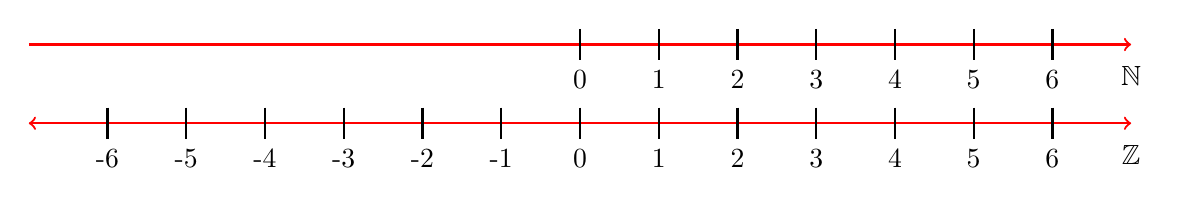
\begin{tikzpicture}
			\draw[thick, red, ->] (0,0) -- (14,0);
			\draw[thick] (7,.2) -- (7,-.2) node[anchor=north] {0};
			\draw[thick] (8,.2) -- (8,-.2) node[anchor=north] {1};
			\draw[thick] (9,.2) -- (9,-.2) node[anchor=north] {2};
			\draw[thick] (10,.2) -- (10,-.2) node[anchor=north] {3};
			\draw[thick] (11,.2) -- (11,-.2) node[anchor=north] {4};
			\draw[thick] (12,.2) -- (12,-.2) node[anchor=north] {5};
			\draw[thick] (13,.2) -- (13,-.2) node[anchor=north] {6};
			\draw (14,-.4) node {$ \N $};
			\draw[thick, red, <->] (0,-1) -- (14,-1);
			\draw[thick] (1,-.8) -- (1,-1.2) node[anchor=north] {-6};
			\draw[thick] (2,-.8) -- (2,-1.2) node[anchor=north] {-5};
			\draw[thick] (3,-.8) -- (3,-1.2) node[anchor=north] {-4};
			\draw[thick] (4,-.8) -- (4,-1.2) node[anchor=north] {-3};
			\draw[thick] (5,-.8) -- (5,-1.2) node[anchor=north] {-2};
			\draw[thick] (6,-.8) -- (6,-1.2) node[anchor=north] {-1};
			\draw[thick] (7,-.8) -- (7,-1.2) node[anchor=north] {0};
			\draw[thick] (8,-.8) -- (8,-1.2) node[anchor=north] {1};
			\draw[thick] (9,-.8) -- (9,-1.2) node[anchor=north] {2};
			\draw[thick] (10,-.8) -- (10,-1.2) node[anchor=north] {3};
			\draw[thick] (11,-.8) -- (11,-1.2) node[anchor=north] {4};
			\draw[thick] (12,-.8) -- (12,-1.2) node[anchor=north] {5};
			\draw[thick] (13,-.8) -- (13,-1.2) node[anchor=north] {6};
			\draw (14,-1.4) node {$ \Z $};
		\end{tikzpicture}
		\caption{The natural numbers and integers ordered number lines.}
	\end{figure}
	Clearly the natural numbers and integers are not ``comprehensive'' in that they have many gaps. This is what led us to define the rational numbers $ \Q $. It isn't immediate just how well the rationals do at covering the holes in the integers. We can get a sense of this by introducing a property of the rationals. 
	\begin{proposition}{(Interspersing of integers by rationals)}
		For any $ x,y\in\Q $ where $ x<y $, there exists a third rational number $ z\in\Q $ such that $ x<z<y $.
	\end{proposition}
	\begin{proof}
		Let there be two rationals $ x,y\in\Q $ such that $ x<y $. We can define the third rational number of interest as $ z=(x+y)/2 $. We can show that $ x<z<y $ by using arithmetic.
		\begin{align*}
			x&<y\\\frac{x}{2}&<\frac{y}{2}\\\frac{x}{2}+\frac{y}{2}&<\frac{y}{2}+\frac{y}{2}\\z&<y
		\end{align*} 
		And we can arrive at $ x<z $ by adding $ x/2 $ to each side of the given inequality.
		\begin{align*}
			x&<y\\\frac{x}{2}&<\frac{y}{2}\\\frac{x}{2}+\frac{x}{2}&<\frac{y}{2}+\frac{x}{2}\\x&<z
		\end{align*} 
	\end{proof}
	\begin{example}
		
		Take the rational numbers $ 0 $ and $ 1 $. Using the construction given in the previous proof we have $$ \frac{0+1}{2}=\frac{1}{2}$$ is between 0 and 1. We can now repeat this process using the pairs $ (0,1/2) $ and $ (1/2,1) $. \begin{align*}
			\frac{0+1/2}{2}=\frac{1}{4}\\\frac{1/2+1}{2}=\frac{3}{4}
		\end{align*}
		We could repeat this process an infinite number of times, in effect ``filling in'' gaps in $ \Z $ by successively taking the average of two rational numbers. Figure 2 shows this process on the unit interval in the rationals. 
		\begin{figure}[h]
			\centering
			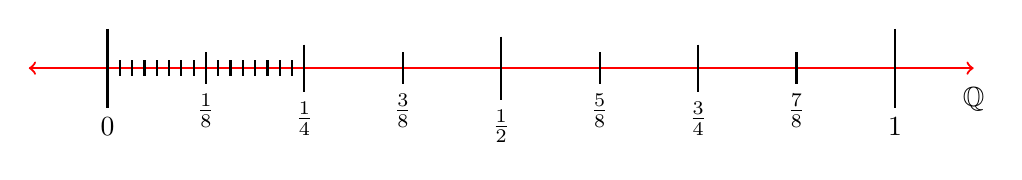
\begin{tikzpicture}
				\draw[thick, red, <->] (-1,0) -- (11,0);
				\draw[thick] (0,.5) -- (0,-.5) node[anchor=north] {0};
				\draw[thick] (5,.4) -- (5,-.4) node[anchor=north] {$ \frac{1}{2} $};
				\draw[thick] (2.5,.3) -- (2.5,-.3) node[anchor=north] {$ \frac{1}{4} $};
				\draw[thick] (7.5,.3) -- (7.5,-.3) node[anchor=north] {$ \frac{3}{4} $};
				\draw[thick] (8.75,.2) -- (8.75,-.2) node[anchor=north] {$ \frac{7}{8} $};
				\draw[thick] (1.25,.2) -- (1.25,-.2) node[anchor=north] {$ \frac{1}{8} $};
				\draw[thick] (6.25,.2) -- (6.25,-.2) node[anchor=north] {$ \frac{5}{8} $};
				\draw[thick] (3.75,.2) -- (3.75,-.2) node[anchor=north] {$ \frac{3}{8} $};
				\draw[thick] (10,.5) -- (10,-.5) node[anchor=north] {1};
				\draw[thick] (0.15625,.1) -- (0.15625,-.1);
				\draw[thick] (0.3125,.1) -- (0.3125,-.1);
				\draw[thick] (0.625,.1) -- (0.625,-.1);
				\draw[thick] (0.46875,.1) -- (0.46875,-.1);
				\draw[thick] (0.78125,.1) -- (0.78125,-.1);
				\draw[thick] (0.9375,.1) -- (0.9375,-.1);
				\draw[thick] (1.09375,.1) -- (1.09375,-.1);
				\draw[thick] (1.40625,.1) -- (1.40625,-.1);
				\draw[thick] (1.5625,.1) -- (1.5625,-.1);
				\draw[thick] (1.71875,.1) -- (1.71875,-.1);
				\draw[thick] (1.875,.1) -- (1.875,-.1);
				\draw[thick] (2.03125,.1) -- (2.03125,-.1);
				\draw[thick] (2.1875,.1) -- (2.1875,-.1);
				\draw[thick] (2.34375,.1) -- (2.34375,-.1);
				\draw (11,-.4) node {$ \Q $};
				
			\end{tikzpicture}
			\caption{}
		\end{figure}\\
		The key question is whether or not this fills \textit{all} the gaps in the integers.
	\end{example}
	While , and more formally , may lead us to believe that the rational numbers have no gaps, this is unfortunately not the case. There are two classic examples that arise from two of the most basic geometric constructions. 
	\begin{example}
		Suppose we have a circle with diameter $ d $ and circumference $ c $. In this case, the ratio give by $ c/d $ is not an element of the rational numbers. This familiar ratio is written as $ \pi $. For the moment, we can take this as fact. We have not yet developed the tools required to proof that $ \pi\notin\Q $, but we will return to this.  
	\end{example}
	\begin{example}
		Suppose there is an isosceles right triangle with legs of length 1, as shown in Figure 3. We want to find the length of the hypotenuse $ x $. 
		\begin{figure}[h]
			\centering
			\begin{tikzpicture}
				\draw[thick] (0,0) -- (8,0);
				\draw[thick] (0,0) -- (0,8);
				\draw[thick] (8,0)--(0,8);
				\draw[thick] (0,0) rectangle (.5,.5);
				\draw[thick] (4,.2)--(4,-.2)node[anchor=north]{1};
				\draw[thick] (.2,4)--(-.2,4)node[anchor=east] {1};
				\draw (4.3,4.3) node {$ x $};
			\end{tikzpicture}
			\caption{}
		\end{figure}\\
		This is a simple application of the Pythagorean Theorem. \begin{align*}
			1^2+1^2&=x^2\\2&=x^2
		\end{align*}
		But this equation has no rational solution, something we can formally prove. 
	\end{example}
	\begin{proposition}
		There exists no rational number $ x $ which satisfies $ x^2=2 $. 
	\end{proposition}
	\begin{proof}
		For the sake of contradiction, suppose that there exists a rational $ x $ which satisfies $ x^2=2 $. If this were the case, we could write $ x=m/n $ for some $ m,n\in\Z $, where $ m $ and $ n $ are not both even.\footnote{Otherwise we could write $ x $ in simpler terms as $ m $ and $ n $ would have a common factor of 2.}
	\end{proof}
	Any $ x $ which does satisfy $ x^2=2 $ would be \textit{irrational}, in that it is not an element of $ \Q $. 
	\begin{definition}\label{def}
		A number is {\color{red}\textit{irrational}} if it is not an element of $ \Q $. 
	\end{definition}
	\noindent There are \textit{many} irrational numbers, each of which is a gap in the rationals (see Figure 4). 
	\begin{figure}[h]
		\centering
		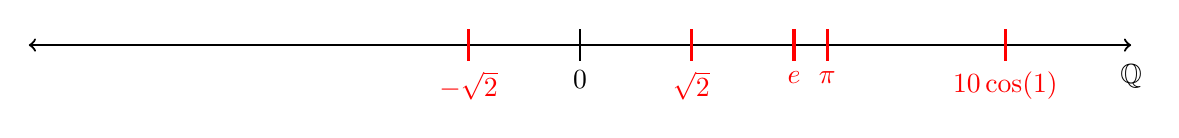
\begin{tikzpicture}
			\draw[thick] (7,.2) -- (7,-.2) node[anchor=north] {0};
			\draw[thick, black, <->] (0,0) -- (14,0);
			\draw (14,-.4) node {$ \Q $};
			\draw[very thick, red ] (10.1415,.2) -- (10.1415,-.2) node[anchor=north] {\color{red}$ \pi $};
			\draw[very thick, red ] (8.4142,.2) -- (8.4142,-.2) node[anchor=north] {\color{red}$ \sqrt{2} $};
			\draw[very thick, red ] (5.5858,.2) -- (5.5858,-.2) node[anchor=north] {\color{red}$ -\sqrt{2} $};
			\draw[very thick, red ] (9.7182,.2) -- (9.7182,-.2) node[anchor=north] {\color{red}$ e $};
			\draw[very thick, red ] (12.403,.2) -- (12.403,-.2) node[anchor=north] {\color{red}$ 10\cos(1) $};
		\end{tikzpicture}
		\caption{}
	\end{figure}\\
	Our goal now becomes defining a set of numbers that includes not only the rationals, but also all of the irrationals. We began with the natural numbers, and then defined a set $ \Z $ which included the additive inverses of the natural numbers. Then we filled more of the gaps in the integers by taking the ratios of integers. We are now faced with the task of defining a set which eliminates the gaps caused by irrational numbers, and doing so eniterly with the set $ \Q $. 
	\subsection{$ \sup $ and $ \inf $}
	Before informally constructing the real numbers, it is worth thinking about why $ \Q $ has these ``holes'', and how it relates to a specific property of sets. It goes without saying that, all the sets of numbers we've discussed up until now have some ordering to them. We can make this formal by defining an ordered set.
	\begin{definition}\label{def}
		An \textit{\color{red}ordered set} is some set $ S $ with a binary relation, denoted by $ < $,\footnote{In this case, ``<'' can mean \textit{any} order. It just so happens that we use the same symbol as the familiar ``less than'' order, because it is the canonical example of such a relation.} which satisfies the following properties:
		\begin{enumerate}
			\item If $ x,y\in S $, then exactly one of the statements $$x<y,\ x=y,\ y<x $$ is true.
			\item If $ x,y,z\in S $, and both $ x<y $ and $ y<z $, then $ x<z $. 
		\end{enumerate}
	\end{definition}  
	The statement $ ``x<y'' $ is read as ``$ x  $ is less than $ y $.''We could also write $ y>x $ instead of $ x<y $. If we were to negative $ y<x $ (``$ y $ is not less than $ x $''), we would arrive at ``y is either greater than $ x $ or equal to $ x $.'' This is denoted as $ y\ge x $. 
	\begin{example}
		The set $ \Q $ is a well ordered set if we define $ < $ in the following way for $ x,y\in\Q $:
		$$ x<y\coloneqq y-x \text{ is a postiive rational number}.   $$ Note that we can only relate objects that belong to $ \Q $. This means that we have no way of comparing rational numbers and the solution to the equation $ x^2=2 $.  
	\end{example}
	We can use the order relation on an ordered set to define bounds on sets.
	\begin{definition}\label{def}
		Suppose $ S $ is an ordered set, and $ E\subseteq S $. If there exists a $ \beta\in S $ such that $ x\le\beta $ for all $ x\in E $, $ E $ is \textit{\color{red}bounded above}, and $ \beta $ is an \textit{\color{red} upper bound} of $ E $. 
	\end{definition}
	\begin{definition}\label{def}
		Suppose $ S $ is an ordered set, and $ E\subseteq S $. If there exists a $ \beta\in S $ such that $ x\ge\beta $ for all $ x\in E $, $ E $ is \textit{\color{red}bounded below}, and $ \beta $ is a \textit{\color{red} lower bound} of $ E $. 
	\end{definition}
	A subtlety in both definitions that is extremely important, is that upper and lower bounds must be elements of the ordered set $ S $. The next example highlights this. 
	\begin{example}
		Take $ \Z $ to be an ordered set with the natural order. Pick the subset $ E=\{-2,-1,2\}\subseteq \Z $. This set has many upper and lower bounds. For upper bounds we have $ 2,3,4,\ldots $. For lower bounds we have $ -2,-3,-4,\ldots
		$. It may be tempting to say that a fraction such as $ 5/2 $ is an upper bound of $ E $, but it is not. This follows from the fact that $ 5/2\notin \Z $, so we have no means of relating it to elements in $ \Z $. In this particular case, there are upper and lower bounds of the set are included in the set. This need not be the case, as the next example shows.  
	\end{example}
	\begin{example}
		Let's look at the ordered set $ \Q $, and subset $ E=\{x\in\Q\mid 0<x<1\}\subseteq \Q $.\footnote{The use of the familiar interval notation of $ (0,1) $ will be properly defined and restricted to the real numbers in the following section.} In this case, each element of $ \{x\in\Q\mid x\le 0\} $ is a lower bound of $ E $, and  each element of $ \{x\in\Q\mid x\ge 1\} $ is an upper bound of $ E $. Even though $ 0,1\notin E $, they are still least and upper bounds of $ E $ respectively. 
	\end{example}
	\begin{remark}
		It is often obvious what exact order we are talking about when referring to an ordered set, like in the case of $ \Q $ and $ \Z $. In these cases, we'll just assume we're using the natural order.  
	\end{remark}
	We now will introduce two definitions that correspond to a special type of upper and lower bound.
	\begin{definition}\label{def}
		Suppose $ S $ is an ordered set, $ E\subseteq S $, and $ E $ is bounded above. We say that $ \alpha $ is a \textit{\color{red}leas- upper-bound} of $ E $ if:
		\begin{enumerate}
			\item $ \alpha $ is an upper bound of $ E $.
			\item If $ \gamma<\alpha $, then $ \gamma $ is not an upper bound of $ E $.
		\end{enumerate}
		Alternatively, we can refer to $ \alpha $ as the \textit{\color{red}supremum} of $ E $, and write $ \alpha=\sup E $
	\end{definition}
	\begin{definition}\label{def}
		Suppose $ S $ is an ordered set, $ E\subseteq S $, and $ E $ is bounded below. We say that $ \alpha $ is a \textit{\color{red}greatest-lower -bound} of $ E $ if:
		\begin{enumerate}
			\item $ \alpha $ is a lower bound of $ E $.
			\item If $ \gamma>\alpha $, then $ \gamma $ is not a lower bound of $ E $.
		\end{enumerate}
		Alternatively, we can refer to $ \alpha $ as the \textit{\color{red}infimum} of $ E $, and write $ \alpha=\inf E $
	\end{definition}
	\begin{remark}
		Both definitions use the definite article \textit{the} before supremum and infimum. This is because they are unique. This is also implied by the use of the superlative \textit{least} and \textit{greatest}. Nevertheless, this is a result of the definition, and can be properly proven. 
	\end{remark}
	
	\begin{example}
		If we return to Example 1.8, where $ E=\{-2,-1,2\}\subseteq\Z $, we have $ \sup E=2 $ and $ \inf E=-2 $. 
	\end{example}
	\begin{example}
		In example 1.9, $ \inf E=0 $ and $ \sup E=1 $.
	\end{example}
	\begin{example}
		Sticking with the set $ \Q$, consider the subset $ E=\{x\in\Q\mid x^2\le 2\}\subseteq \Q $. This set has no supremum, because the number satisfying $ x^2=2 $ is not an element of $ \Q $ (as shown in Proposition 1.2). We will formally prove this fact shortly. 
	\end{example}
	It is no coincidence that a subset of $ \Q $ fails to have a supremum, because of one of the ``holes'' in $ \Q $. The following definition will help us formalize this relationship. 
	\begin{definition}\label{def}
		Let $ S $ be an ordered set. If for all $ E\subseteq S $, where $ E $ is nonempty and bounded from above, $ \sup E $ exists, then $ S $ has the \textit{\color{red}least-upper-bound} property. 
	\end{definition}
	The least-upper-bound property ensures that any nontrivial subset of an ordered set has a supremum in that ordered set. We could define an equivelent property known as the greatest-lower-bound property. The next two propositions serves as nice examples of the least-upper-bound property, or lack there of,  in action.
	\begin{proposition}
		The set $ \Z $ has the least-upper-bound property.
	\end{proposition}
	The idea behind the following proof takes advantage of the fact that $ \Z $ is discrete. For some set $ E\subseteq \Z $, we can always just look at an upper bound of it, and keep subtracting $ 1 $ until the resulting number is in $ E $. Then we will have found our upper bound.
	\begin{proof}
		We will show that an arbitrary nontrivial set $ E\subseteq \Z $ has a supremum. Let $ x\in E $, and $ \beta $ be an upper bound of $ E $. We know that $ \beta\ge x $ for all $ x\in E $ We can show that $ \sup E $ exists via induction on $ \beta-x $ for our arbitrary $ x\in E $. Our base case is when $ \beta-x=0 $. If this holds, then $ \beta\in E $, so $ \beta\in\Z $ and $ \sup E=\beta $. Now suppose that this statement holds when $ \beta-x=k $ for $ k\in\N $ (this is our induction hypothesis). It is either the case that $ \beta\in E $ or $ \beta\notin E $. If $ \beta\in E $, then $ \sup E=\beta $. If $ \beta \notin E $, then let $ \beta'=\beta -1 $. Then $ \beta' $ is an upper bound of $ E $, and $$\beta'-x=\beta-1-x=\beta-x-1=k+1=1=k .$$ By the induction hypothesis, $ \sup E $ exists.   
	\end{proof}
	\begin{proposition}
		The set $ \Q $ does not have the least-upper-bound property.
	\end{proposition}
	To prove this, we will first establish that $ 2 $ is an upper bound of the set defined in Example 1.12, and then show the set has no supremum via contradiction.
	\begin{proof}
		If suffices to find a single subset of $ \Q $ which fails to have a supremum. Let that set be $ E=\{x\in\Q\mid x^2\le 2\} $. 
		\begin{enumerate}
			\item Suppose for contradiction that $ 2 $ is not an upper-bound of $ E $. Then there exists an $ x\in E $ such that $ x>2 $. This would imply that $ x^2>4 $, which contradicts the assumption that $ x \in E $. 
			\item Suppose for contradiction that $ E $ has a supremum, and that $ \sup E=\alpha $ for $ \alpha\in\Q $. Define a new rational number $ y\in \Q $ as 
			\begin{equation}
				y=\alpha-\frac{\alpha^2-2}{x+2}=\frac{2(\alpha+1)}{\alpha+2}.
			\end{equation}
			Squaring this and subtracting $ 2 $ gives 
			\begin{equation}
				y^2-2=\frac{4(\alpha+1)^2}{(\alpha+2)^2}-\frac{2(\alpha+2)^2}{(\alpha+2)^2}=\frac{2(\alpha^2-2)}{(\alpha+2)^2}.
			\end{equation} We can use $ y $ to reach a contradiction in each possible case, those being: $ \alpha^2<2 $, $ \alpha^2=2 $, $ \alpha^2>2 $.
			\begin{enumerate}
				\item Suppose that $ \alpha^2<2 $. This means that $ \alpha^2-2<0 $, so Equation (1) implies that $ y>\alpha $. At the same time, Equation (2) implies that $ y^2-2<0 $, which means $ y^2<2 $. This gives that $ y\in E $, despite the fact that $ \alpha<y $. This contradicts the fact that $ \alpha $ is an upper-bound of $ E $
				\item Suppose $ \alpha^2=2 $. We already know this cannot be the case by Proposition 1.2. 
				\item  Finally, assume that $ \alpha^2>2 $, giving $ \alpha^2-2=0 $. Equation (1)	implies $ y<\alpha $ while Equation (2) implies $ y^2-2>0 $, meaning $ y^2>2 $. This establishes $ y $ as an upper bound for $ E $, but $ y<\alpha $, which contradicts $ \sup E=\alpha $.  
			\end{enumerate}
		\end{enumerate}
	\end{proof}
	The ``holes'' in $ \Q $ are a result of $ \Q $ not having the least-upper-bound property. In order to perform calculus, we need a set that has this property, otherwise things like continuity and differentiation would not work. This property is not sufficient in and of itself though. If that were the case then we would have stopped extending out set of numbers at $ \Z $. We want a set of numbers as ``comprehensive'' as $ \Q $, but with the least-upper-bound property. It turns out, that this (and a whole lot more) is what we will get from the real numbers.  
	\subsection{The Real Numbers}
	We will now construct the real numbers using only $ \Q $. First, we will define the algebraic structure that the real numbers will take on.
	\begin{definition}\label{def}
		A \textit{\color{red}field} is a set $ F $ with two operations, addition and multiplication, which satisfy the following axioms for all $ x,y,z\in F $:
		\begin{enumerate}
			\item Axioms for addition:
			\begin{enumerate}
				\item $ x+y\in F $ (closed under addition)
				\item $ x+y=y+x $ (commutative)
				\item $ (x+y)+z=x+(y+z) $ (associative)
				\item There exists an element $ 0\in F $ such that $ 0+x=x $ (identity element)
				\item There exists an element $ -x\in F $ such that $ x+(-x)=0 $ (inverse element)
			\end{enumerate}
			\item Axioms for multiplication:
			\begin{enumerate}
				\item $ xy\in F $ (closed under multiplication)
				\item $ xy=yx $ (commutative)
				\item $ (xy)z=x(yz) $ (associative)
				\item There exists an element $ 1\in F $ such that $ 1x=x $ (identity element)
				\item If $ x\neq 0 $, there exists an element $ 1/x\in F $ such that $ x(1/x)=1 $ (inverse element)
			\end{enumerate}
			\item The distributive property:
			$$ x(y+z)=xy+xz$$
		\end{enumerate}
	\end{definition}
	The study of fields is its own entire subject in math, and lives within the discipline if abstract algebra. For more details about fields, see \cite{dummit2004abstract}. These axioms can be used to reach several familiar conclusions about arithmetic in fields, and can be found as formal propositions in \cite{rudin1964principles}. A more specific type of field is that which is also an ordered set.
	\begin{definition}\label{def}
		An \textit{\color{red} ordered field} is a field $ F $ such that
		\begin{enumerate}
			\item $ x+y<x+z $ if $ x,y,z\in F $ and $ y<z $,
			\item $ xy>0 $ if $ x,y\in F $, $ x>0 $, and $ y>0 $. 
		\end{enumerate}
	\end{definition}
	\begin{example}
		The set $ \Q $ is an ordered field. 
	\end{example}
	
	Our goal is now to construct an ordered field which not only contains $ \Q $, but also has the least-upper-bound property. In order to do this we'll use the fact that $ \Q $ has ``holes'' in it. We'll form a pair of set $ (A,B) $ that partition $ \Q $ such that each of these partitions corresponds to a real number. 
	
	\begin{definition}\label{def}
		A \textit{\color{red}Dedekind cut} $ x=(A,B) $ is a pair of subsets $ A,B\subseteq \Q $ satisfying the following:
		\begin{enumerate}
			\item $ A\cup B=\Q $, $ A\cap B=\emptyset $, $ A\neq\emptyset $, and $ B\neq\emptyset $.
			\item If $ a\in A $ and $ b\in B $, then $ a<b $.
			\item $ A $ contains no largest element.
		\end{enumerate}
	\end{definition} 
	\begin{example}
		Let $ A=\{y\in \Q \mid y<0\} $ and $ B=\{y\in\Q\mid y\ge 0\} $. Our cut is $ x=(A,B) $, and can be seen in Figure 5.
		\begin{figure}[h]
			\centering
			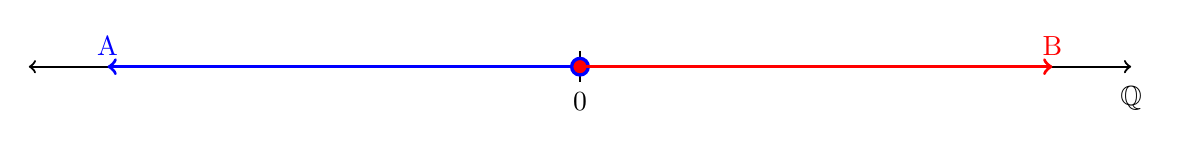
\begin{tikzpicture}
				\draw[thick] (7,.2) -- (7,-.2) node[anchor=north] {0};
				\draw[thick, black, <->] (0,0) -- (14,0);
				\draw (14,-.4) node {$ \Q $};
				\draw[ very thick, blue, ->] (7,0) -- (1,0) node[anchor=south] {A};
				\filldraw[color=blue, fill=red, very thick] (7,0) circle (3pt);
				\draw[ very thick, red, ->] (7,0) -- (13,0) node[anchor=south] {B};
				
			\end{tikzpicture}
			\caption{Dedekind cut corresponding to $ 0\in\Q $.}
		\end{figure}
		This cut uniquely represents $ 0\in\Q $, as no other cut can be defined in this way ``at'' $ 0 $. 
	\end{example}
	\begin{example}
		Perhaps a better example is the cut defined by $ A=\{q\in\Q\mid q\le 0\text{ or }q^2<2 \} $ and $ A=\{q\in\Q\mid q> 0\text{ or }q^2>2 \} $. This cut corresponds to the solution of the equation $ x^2=2 $.  
	\end{example}
	\begin{definition}\label{def}
		A \textit{\color{red}real number} is a Dedekind cut in $ \Q $. The set of real numbers is denoted by $ \R $. 
	\end{definition}
	\begin{definition}\label{def}
		A real number $ x=(A,B) $ is a \textit{\color{red}rational number} if $ B $ contains a smallest element (namely $ x $).
	\end{definition}
	\begin{definition}\label{def}
		A real number $ x=(A,B) $ is a \textit{\color{red}irrational number} if $ B $ contains no smallest element.
	\end{definition}
	\begin{example}
		The cut defined by $ A=\{y\in \Q \mid y<0\} $ and $ B=\{y\in\Q\mid y\ge 0\} $ is rational, as $ B $ has a smallest element in the form of $ 0 $.  
	\end{example}
	\begin{example}
		The cut defined by $A=\{q\in\Q\mid q\le 0\text{ or }q^2<2 \} $ and $ A=\{q\in\Q\mid q> 0\text{ or }q^2>2 \} $ has no smallest element. Therefore it is an irrational number. We will denote this particular number as $ \sqrt{2} $. 
	\end{example}
	Now that we have properly defined $ \R $, we can \textit{finally} refer to the quantity $ \sqrt{2} $! It is no longer a mysterious solution to an equation, and is well defined in $ \R $. This is a relatively small payoff, but the real rewards are the two following theorems. These are the main results of this section, and are of the utmost importance. The first will allow us to perform operations on $ \R $, and the second will play a key role in proving familiar theorems from calculus. The proof of the first result is rather long, and not very informative, so it is omitted. It is important to understand \textit{how} it would be proved though. Before the big reveal, we will define an order on $ \R $
	\begin{definition}\label{def}
		Given real numbers $ x=(A,B) $ and $ y=(C,D) $, we define the following order:$$x\le y\coloneqq A\subseteq C .$$ The inequality is strict if $ A\subseteq C $. 
	\end{definition}
	\begin{example}
		Let $ x=2=(A,B)=(\{y\in \Q \mid y<2\},\{y\in\Q\mid y\ge 2\})$, and $ y=3=(C,D)=(\{z\in \Q \mid z<3\},\{z\in\Q\mid z\ge 3\})$. It should come as no surprise that $ 2<3 $, but this is because $ A\subseteq C $.  
	\end{example}
	\begin{theorem}
		The set $ \R $ is an ordered field containing $ \Q $.
	\end{theorem}
	\begin{proof}
		See the appendix of chapter 1 in \cite{rudin1964principles}. The idea is that addition and multiplication of cuts must be define, and the all the axioms of fields and ordered fields must be verified using the cut definition of a real number. 
	\end{proof}
	\begin{theorem}[Completeness of the real numbers]
		The set $ \R $ has the least-upper-bound property.
		\begin{proof}
			We will show an arbitrary nonempty subset of $ \R $ has a supremum. Let $ E\subseteq \R $, where $ A\neq\emptyset $, have the upper bound $ \beta\in\R $. We may write $ \beta $ as a Dedekind cut, $ \beta=(A,B) $. Additionally, we may express each $ \alpha\in E $ as a cut $ \alpha=(L_\alpha,U_\beta) $. Now we will construct a real number by taking the union of all $ L_\alpha $.
			$$ \gamma=\left(\bigcup_{\alpha\in E}L_\alpha,\Q\backslash \bigcup_{\alpha\in E}L_\alpha\right)=(L,\Q\backslash
			L)=(L,U)$$  
			I claim that $ \sup E=\gamma $.
			
			First we must verify that $ \gamma\in\R $ by showing that $ (L,U) $ is a valid Dedekind cut, and satisfies the requirements of Definition 1.13: 
			\begin{enumerate}
				\item The set $ E $ is nonempty, so there exists at least one $ \alpha=(L_\alpha,U_\alpha)\in E $. Because $ L_\alpha\neq\emptyset $ and $ U_\alpha\neq\emptyset $ by definition 1.13, we have $ L\neq\emptyset $ and $ U\neq\emptyset $. By the definition of $ U $ as $ \Q\backslash L $, we have that $  L\cup U=\Q$ and $ L\cap U=\emptyset $. Therefore $ \gamma\in\R $. By construction, $ \alpha\le\gamma $ for all $ \alpha\in E $, making $ \gamma $ an upper bound. 
				\item To show that it is the least-upper-bound, we will now show any number lesser than it cannot be an upper bound. Now suppose $ \delta <\gamma $. This means $  C\subseteq L $, where $ \delta $ is expressed as a cut $ \delta=(C,D) $. This means there exists some $ s\in L $ such that $ s\notin C $. But $ s\in L $, so it is in $ L_\alpha $ for some $ \alpha\in E $. Hence, $ C\subseteq L_\alpha $, giving $ \delta <\alpha $. This shows that $ \delta $ is not an upper bound, meaning $ \sup E =\gamma$.
			\end{enumerate}
		\end{proof}
	\end{theorem}
	
	\begin{example}
		Consider the set of real numbers $ E=\{-1,-1/2,-1/3,-1/4,\ldots\} $. What is the supremum of this set? Intuitively, it should be $ 0 $, but we can verify this by constructing it like we did in the previous proof. Each number in $ E $ corresponds to a cut $ (L_n,U_n) $, for $ L_n=\{x\in\Q\mid x<-1/n\} $ and $ U_n=\{x\in\Q\mid x\ge -1/n\} $, where $ n\in\N $. Our supremum is $$\gamma=\left(\bigcup_{n\in \N}\{x\in\Q\mid x<-1/n\},\Q\backslash \bigcup_{n\in \N}\{x\in\Q\mid x<-1/n\}\right)=(\{x\in\Q\mid x<0\},\{x\in\Q\mid x\ge0\}). $$ Therefore, $ \gamma=0 $.  
	\end{example}
	You will often here the real numbers referred to as ``complete'' because they have the least-upper-bound property. This is because the least-upper-bound property ensures there are no ``gaps'' in the real line like there are in $ \Q $. Theorem 1.2 may be the most important result in real analysis. Remember it well, as it will be used often. Most disciplines in math build on themselves over time, and the fact that $ \R $ has the least-upper-bound property will be our foundation. One could argue it is $ \R $'s defining property.  
	
	Finally, we will adopt the familiar notation of intervals in $ \R $, and add make an important addition to $ \R $. 
	\begin{definition}\label{def}
		We will use the following notation to refer to \textit{\color{red} intervals} of $ \R $:
		\begin{align*}
			(a,b)=\{x\in\R\mid a<x<b\}\\
			[a,b)=\{x\in\R\mid a\le x<b\}\\
			(a,b]=\{x\in\R\mid a<x\le b\}\\
			[a,b]=\{x\in\R\mid a\le x\le b\}
		\end{align*}
		for $ a<b $. 
	\end{definition}
	\begin{definition}\label{def}
		The \textit{\color{red}extended real number system} consists of the real field $ \R $ and two symbols: $ \infty $, and $ -\infty $. The original order of $ \R $ is preserved, and we define $$ -\infty <x<\infty$$ for all $ x\in\R $. We will denote the extended real numbers as $ \overline{\R} $.  
	\end{definition}
	The extended real numbers do not form a proper field, but we can adopt some conventions for arithmetic using $ \infty $ and $ -\infty $ for $ x\in\R $:
	\begin{enumerate}
		\item $ x+\infty=\infty $, $ x-\infty=-\infty $, $ x/\infty=x/-\infty=0 $. 
		\item For $ x>0 $, $ x(\infty)=\infty $, and $ x(-\infty)=-\infty $.
		\item For $ x<0 $, $ x(\infty)=-\infty $, and $ x(-\infty)=\infty $.
	\end{enumerate}
	The addition of an upper and lower bound on $ \R $ make the set $ \overline{\R} $ easier to work with in certain situations.\footnote{What we are really doing is working with $ \overline{\R} $ because it is a complete lattice. A complete lattice is a partially ordered set in which every subset has an infimum or supremum. The real line is not a complete lattice, as any set of the form $ (a,\infty)\subset\R $ has no supremum.} The most immediate result of working in $ \overline{\R} $ is that \textit{every} subset of $ \R $ has a supremum, not just bounded ones (the latter case being the only one stipulated by the least-upper-bound property). 
	\subsection{Properties of $ \R $}
	The importance of Theorem 1.2 can not be understated. It is perhaps \textit{the} defining property of $ \R $, and it gives rise to numerous results in analysis. For now, we can use it to prove two additional properties of $ \R $.
	\begin{theorem}[Archimedean property of $ \R $]
		For $ x,y\in \R $ where $ x>0 $, there exists an $ n\in\N $ such that $ nx>y $.
	\end{theorem}   
	\begin{proof}
		Let $ A $ be the set of all $ nx $ for $ x\in\R $ and $ n\in\N $, where $ x>0 $. For contradiction, suppose that there exists no such $ n\in\N $ such that $ nx>y $ for $ y\in\R $. This makes $ y $ an upper bound of $ A $. By the completeness of $ \R $, $ \sup A=\alpha $ exists. Since $ x>0 $, $ \alpha-x<\alpha $, and $ a-x $ is not an upper bound of $ A $. This means there exists an $ m\in\N $ such that $ a-x<mx $. But this would imply $ \alpha<mx+x=m(x+1) $, where $ (m+1)x\in A $. This contradicts the fact that $ \alpha $ is an upper bound of $ A $. 
	\end{proof}
	\begin{example}
		Suppose $ x=10 $ and $ y=213 $. By the Archimedean property of $ \R $, we know there exists a multiple of $ 10 $ that is greater than $ 213 $. $$ 10(22)=220>213$$  
	\end{example}
	\begin{theorem}[$ \Q $ is dense in $ \R $]
		For $ x,y\in \R $ where $ x<y $, there exists a $ p\in\Q $ such that $ x<p<y $. 
	\end{theorem}  
	\begin{proof}
		We have $ x<y $, giving $ y-x>0 $. By the Archimedean property (Theorem 1.3), there exists an $ n\in\N $ such that 
		\begin{equation}
			n(y-x)>1.
		\end{equation}
		We can use Theorem 1.3 to find $ m_1,m_2\in\N $ for which:
		\begin{align*}
			m_1>nx,\\m_2>-nx.
		\end{align*}
		We can combine these two inequalities to conclude $ -m_2<nx<m_1 $. This implies there exists an $ m\in\N $ (with $ -m_2\le m\le m_1 $) such that \begin{equation}
			m-1\le nx<m.
		\end{equation}  
		If we combine $ (3) $ and $ (4) $ we get $$ nx<m\le 1+nx<ny.$$ Dividing by $ n $ (which is positive) gives $ x<\frac{m}{n}<y$. 
	\end{proof}
	The density of $ \Q $ in $ \R $ is both surprising and useful for constructing examples. In practice, it means that every irrational number has a rational number arbitrarily close to it. We can approximate any number in $ \R $ arbitrarily well with a rational number.
	\begin{example}
		We will now mimic the proof of Theorem 2.4 with actual numbers. We will find a rational $ p\in\Q $ such that $ e<p<\pi $.\footnote{You shouldn't even need to perform the construction to arrive at an answer, as $ e $ and $ \pi $ are not particularly ``close'' to each other. We could for instance take $ p=3 $. } We have $ \pi-e>0 $. We know $$ 3(\pi-e)>1 .$$ Next we pick whole numbers $ m_1=9 $ and $ m_2=8 $, and get the inequality $ 8<3e<9 $. Now take $ m $ to be $ 9 $ and reach our final inequality of $$ 3e<9<1+3e <3\pi.$$ Dividing by $ n=3 $ gives our desired rational number is $ 9/3=3 $.  
	\end{example}
	\begin{example}
		Let $ \sqrt{2}\in\R $, and let $ \varepsilon>0 $.\footnote{This is the first time we're using the infamous $ \varepsilon $. It just stands in for any arbitrarily small positive number.} By the density of $ \Q $ in $ \R $, there exists $ p\in\Q $ such that $ \sqrt{2}-\varepsilon<p<\sqrt{2} $. This will hold \textit{for all} $ \varepsilon>0 $ so as we let $ \varepsilon $ become smaller and smaller, we will have an increasingly accurate rational approximation of $ \sqrt{2} $.
	\end{example}     
	\subsection{Cardinality}
	So far, I've been intentional in avoiding any discussion of the size of the sets we have been working with. When constructing $ \Z $ from $ \N $, it was never stated that $ \Z $ was somehow ``bigger'' than $ \N $. All we know is that $ \Z $ has elements that $ \N $ does not. The same can be said for $ \Z $ and $ \Q $, or $ \Q $ and $ \R $. It is now time that we turn our attention to this matter, and more generally the size, or ``cardinality'' of sets. 
	
	Determining the size of a set amounts to counting the number of elements in that set. But how do we make the notion of counting formal? We will do this with functions. Before formally defining anything, consider how you may count something. If you are tasked with counting the number of elements in the set $ X=\{a,b,c\} $, you're answer will surely by 3. How did you get that number? You said assigned the number $ 1 $ to $ a $, $ 2 $ to $ b $, and $ 3 $ to $ c $. We should note three different things about this process:
	\begin{enumerate}
		\item Each number we use is from $ \N $.
		\item Each element of $ X $ is assigned a number. We wouldn't have counted properly if we skipped some element. 
		\item No number in $ \N $ is assigned to multiple elements in $ X $. We do not want to count multiple elements as a single element.
	\end{enumerate}
	This process of assigning elements in $ \N $ to those in $ X $ is shockingly similar to the notion of a function, as we are mapping elements from one set to those in another set. Furthermore, the properties we must obey while counting have their own analogous forms with functions: surjectivity, and injectivity. For this reason, we will use functions to formalize the size of a set.
	
	First, we will address the abstract case of when two sets have the same number of elements, and then we will transition to the size of sets.
	\begin{definition}\label{def}
		The \textit{\color{red}cardinality} of a set $ X $, denoted $ |X| $, is the number of elements that belong to the set.   
	\end{definition} 
	\begin{definition}\label{def}
		Two sets $ X $ and $ Y $ have \textit{\color{red}the same cardinal number} if there exists a bijection $ f:X\to Y $ from $ X $ to $ Y $.  
	\end{definition} 
	\begin{proposition}
		Define the relation $ X\sim Y $ \textit{only if} $ X $ and $ Y $ have the same cardinal number ($ |X|=|Y| $). The relation $ \sim $ is an equivalence relation. 
	\end{proposition} 
	\begin{proof}
		We have that $ X\sim X $ by letting $ f:X\to X $ be $ f(x)=x $, so $ \sim $ is reflexive. If $ X\sim Y $, there exists a bijection $ f:X\to Y $. Since $ f $ is a bijection, it has an inverse $ f^{-1}:Y\to X $. This inverse is itself a bijection, so $ Y\sim X $, making $ \sim $ symmetric. Lastly, assume $ X\sim Y $ and $ Y\sim Z $. We have bijections $ f:X\to Y $ and $ g:Y\to Z $. The composition of two bijections is a bijection, so $ h:X\to Z $ is a bijection. This makes $ \sim $ transitive.  
	\end{proof}
	\begin{example}
		Let $ X=\{1,2,3\} $ and $ Y=\{\sqrt{2},e,\pi\} $. We can define $ f:X\to Y $ as $$ f(x)=\begin{cases}
			\sqrt{2}\text{ if }x=1\\e\text{ if }x=2\\\pi\text{ if }x=3
		\end{cases}.$$
		\begin{figure}[h!]
			\centering
			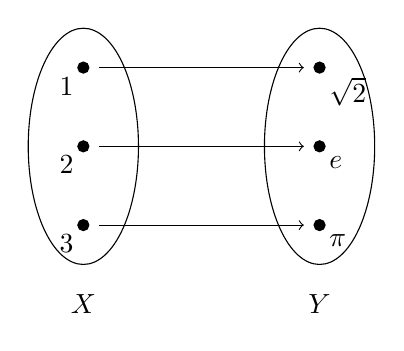
\begin{tikzpicture}
				\draw (0,0) ellipse (0.7cm and 1.5cm);
				\draw (3,0) ellipse (0.7cm and 1.5cm);
				\filldraw (0,0) circle (2pt) node[anchor=north east] {$ 2 $};
				\filldraw (0,1) circle (2pt) node[anchor=north east] {$ 1 $};
				\filldraw (0,-1) circle (2pt) node[anchor=north east] {$ 3 $};
				\filldraw (3,0) circle (2pt) node[anchor=north west] {$ e $};
				\filldraw (3,1) circle (2pt) node[anchor=north west] {$ \sqrt{2} $};
				\filldraw (3,-1) circle (2pt) node[anchor=north west] {$ \pi $};
				
				\draw (0,-2) node {$ X $};
				\draw (3,-2) node {$ Y $};
				\draw[->] (0.2,0) -- (2.8,0) ;
				\draw[->] (0.2,1) -- (2.8,1) ;
				\draw[->] (0.2,-1) -- (2.8,-1) ;
			\end{tikzpicture}
			\caption{Bijection $ f:X\to Y $.}
		\end{figure}  \\
		This function is clearly a bijection, and we have that $ |X|=|Y| $.
	\end{example} 
	\begin{example}
		Let $ \Z^-=\{x\in\Z\mid x<0\} $ and $ \Z^+=\{x\in\Z\mid x>0\} $. There exists a very natural bijection between these sets, namely that which maps each element in $ \Z^+ $ to it's negative counterpart in $ \Z^- $. Formally, $ f:\Z^+\to\Z^- $ is define as $ f(x)=-x $. This function is clearly a bijection, and its existence shows that $ |Z^+|=|Z^-| $. There are the same number of positive integers as negative integers  
	\end{example}
	\begin{remark}
		Because $ f:X\to Y $ is a bijection, it doesn't matter which set is the domain and which set is the codomain. A function is invertible if and only if it is a bijection, and a functions inverse is a bijection, so we would just have $ f^{-1}:Y\to X $ if we picked the sets in the other order. In example 2.23, we could have instead assigned each negative integer to it's positive counterpart and had $ f:\Z^-\to\Z^+ $. In this case we would still have $ f(x)=-x $, as this particular function is its own inverse! 
	\end{remark}
	
	As discussed earlier, counting is intrinsically linked to the set of natural numbers $ \N $. We will now make this formal by defining three types of sets: finite sets, countably infinite sets, and uncountably infinite sets.
	\begin{definition}\label{def}
		A set $ X $ is \textit{\color{red}finite} if there exists a subset of the whole numbers $ N\subseteq \N $ for which $ X $ and $ N $ have the same cardinal number.
	\end{definition} 
	\begin{definition}\label{def}
		A set $ X $ is \textit{\color{red}countably infinite} if $ X $ has the same cardinal number as $ \N $. Alternatively, $ X $ is countably infinite if there exists a bijection $ f:X\to\N $. This is sometimes denoted as $ |X|=\aleph_0 $.\footnote{This symbol is an ``aleph'', and is the first letter of the Hebrew alphabet.} 
	\end{definition}
	\begin{definition}\label{def}
		A set $ X $ is \textit{\color{red}countable} if it is countably infinite or finite.
	\end{definition}
	\begin{remark}
		From here on out, I'm going to use countable and countably infinite interchangeably, as nearly all the sets we are interested in are infinite.  
	\end{remark}
	\begin{definition}\label{def}
		A set $ X $ is  \textit{\color{red}uncountably infinite} (or uncountable) if it is neither finite nor countably infinite.
	\end{definition}
	Before jumping into examples, let's unpack some of this. Finiteness and countable infiniteness depend on whether a set has the same cardinal number as a subset of $ \N $ or $ \N $ itself. This means we can find a bijection between the set and a subset of $ \N $ or $ \N $ itself. Definition 1.22 and 1.23 are often presented in terms of this hypothetical bijection. Secondly, two of these definitions involve infinity. A set can be either countably infinite or uncountably infinite. In a sense, some infinite sets have so many elements that they cannot even be counted, and are ``bigger'' than other uncountable sets! These two concepts of infinity will show up constantly in real analysis. Hopefully examples will make this clear. Some of the following examples are so important that they will be presented as formal results. 
	\begin{example}
		We will modify Example 2.22. Let Let $ X=\{\sqrt{2},e,\pi\} $ and $ N=\{1,2,3\}\subseteq \N$. Take our bijection to be the inverse of the function defined previously in Example 2.22. This shows that $ X $ is finite, and $ |X|=3 $. 
	\end{example}
	\begin{proposition}
		The set $ \N $ is countably infinite.
	\end{proposition}
	\begin{proof}
		Define $ f:\N\to\N $ as $ f(n)=n $. This function is clearly a bijection. 
	\end{proof}
	\begin{proposition}
		The set $ \Z $ is countably infinite.
	\end{proposition}
	Before proving this result, it's worth acknowledging that it seem paradoxical. How can it be that $ \Z $ is the same size as $ \N $, despite $ \Z $ being defined as $ \N $ plus more elements? It would make more sense for $ \Z $ to have twice the cardinality as $ \N $, but this is not the case. The result may sit better if you consider just how we would count $ \Z $. If you started at $ 1\in\Z $, followed by $ 2\in\Z $, etc. then you would miss all the negative numbers! Instead, we need to be clever in the order in which we count $ \Z $. We will instead count in the following order: $ 0,1,-1,2,-2,\ldots $. We could count like this forever and never run out of $ \N $, and never miss any elements of $ \Z $. This is why we have $ |\N|=|\Z| $. 
	\begin{proof}
		Recall that we can select either $ \Z $ or $ \N $ to be the domain of our bijection. We will define $ f:\N\to\Z $ as
		$$f(n)=\begin{cases}
			\frac{n}{2}\text{ if }n\text{ is even}\\
			-\frac{n-1}{2}\text{ if }n\text{ is odd}
		\end{cases}.$$
		This function counts $ \Z $ in the aforementioned manner of alternating between positive and negative integers. We now will verify that $ f $ is a bijection, by showing it is injective and surjective.\footnote{It would be quicker to show $ f $ has an inverse, but that approach is not as instructive.} Let $ y\in\Z $, and pick $ x\in\N $ such that $ x=2y $ if $ y $ is even, and $ x=-2y+1 $ if $ y $ is odd. This choice of $ x\in\N $ gives $ f(x)=y $, so $ f $ is surjective. Now suppose that $ f(x_1)=f(x_2) $. If $ x_1/2=x_2/2 $, then $ x_1=x_2 $. If $ -(x_1-1)/2=-(x_2-1)/2 $, then $ x_1=x_2 $. Therefore, $ f $ is injective.
	\end{proof}
	An even more surprising result is that not only $ |\N|=|\Q| $, but also $ |\N|=|\Z|=|\Q| $! Even if we add every possible fraction to the integers, the size of our set remains the same.
	\begin{theorem}
		The set $ \Q $ is countably infinite. 
	\end{theorem}
	
	\begin{proof}
		We can enumerate the rational numbers in the following way: $$ \frac{0}{1},\frac{1}{1},\frac{-1}{1},\frac{1}{2}, \frac{1}{3}, \frac{2}{1}, \frac{-2}{1}, \frac{-1}{3}, \frac{1}{4}, \frac{1}{5}, \frac{-1}{4}, \frac{2}{3},\ldots $$ This particular ordering can be seen in Figure 7. The red arrows in Figure 7 show the order in which we count, and it becomes evident that we will eventually count every possible fraction. Note that we only count fractions which are expressed in simplest terms, with others in gray. 
		\begin{figure}[h!]
			\centering
			\includegraphics[width=0.9\linewidth]{figures/Qcountable}
			\caption{}
			\label{fig:qcountable}
		\end{figure}
	\end{proof}
	It may not be a surprise that it is not possible to count $ \R $. This puts $ \R $ in our second category of infinite sets, uncountably infinite.
	\begin{theorem}
		The set $ \R $ is uncountably infinite. 
	\end{theorem}
	The proof of this theorem is a classic, and is due to Cantor. 
	\begin{proof}
		Suppose for contradiction that $ \R $ were countably infinite. There exists a bijection $ f:\N\to\R $, and we make a table of values the function takes on (see Table 1). Table 1 is just an example of what such a bijection may look like, and the exact values are moot.
		\begin{table}[h!]
			\centering
			\begin{tabular}{cc}
				$ n\in\N  $       & $ f(n)\in\R $              \\ \hline
				1        & $4.3214875\ldots$ \\
				2        & $1.4918401\ldots$           \\
				3        & $3.0194510\ldots$                   \\
				4        & $9.0194510\ldots$                  \\
				5        & $0.3917293\ldots $               \\
				6        & $ 5.9184017\ldots $\\
				7        & $ 1.9284010\ldots $                \\
				$\vdots$ & $\vdots$         
			\end{tabular}
		\end{table}
		Because $ f $ is a bijection, this table should go on forever, and count every element of $ \R $. To reach a contradiction, we will simply show there exists a real number that was not counted.\footnote{There in fact exist \textit{many} that would go uncounted, but it suffices to find just one.} ``Construct'' this uncounted real number in the following way: let the $ n^{th} $ digit (decimal places included) take on the value of the $ n^{th}$ digit of $ f(n) $ minus one (if it is $ 0 $, set it to $ 9 $). For Table 1, the first digit would be the first digit of $ f(1) $ minus 1, which is $ 4-1=3 $. The second digit would be the second digit of $ f(2) $ minus 1, which is $4-1=3$. We repeat this process for all $ n\in\N $, and in our case we get $$3.308690\ldots $$
		By construction, the $ n^{th} $ digit of this number is different from at least one of the $ n^{th} $ digits of $ f(n) $. This holds for every $ n\in\N $, so this number is different from every value of $ f(n) $, and was therefore not counted.  
	\end{proof}
	\begin{corollary}
		Every infinite subset of $ \R $ is uncountable.
	\end{corollary}
	\begin{example}
		Every interval $ [a,b]\subseteq\R $ is uncountable. 
	\end{example}
	Now that we've seen which familiar sets are and are not countable, there are several key results involving the cardinality of sets that deserve attention. These will establish what happens to the cardinality of sets when different set operations are performed. 
	\begin{proposition}
		Let $ \{E_n\} $, $ n\in\N $, be a sequence of countably infinite sets, and let $ E=\cup_{n\in N}E_n $ be a countable union. The set $ E $ is countably infinite. 
	\end{proposition}
	\begin{proof}
		We will prove via induction. Our base case is $ n=2 $. The sets $ E_1 $ and $ E_2 $ are countably infinite, so there exists bijections $ f:\N\to E_1 $ and $ g:\N\to E_2 $. Without loss of generality, assume $ E_1\cap E_2=\emptyset $.\footnote{Otherwise, we could replace $ E_1 $ with $ E_1\backslash E_2 $.} Define $ h:\N\to E_1\cup E_2 $ as $$ h(k)=\begin{cases}
			f(k/2)\text{ if }k  \text{ is even}\\
			g((k+1)/2)\text{ if }k  \text{ is odd}
		\end{cases}. $$ This function counts the elements in the set by alternating between those in $ E_1 $ and $ E_2 $ (like in the proof of Proposition 1.7). The function $ h $ is a bijection, so $ E_1\cup E_2 $ is countably infinite. Now suppose this holds for $ E_1,\ldots E_{n-1} $. We can write $ E $ as a union of two countably infinite sets by taking the union over $ E_1,\ldots E_{n-1} $, which is countably infinite by the induction hypothesis. 
		\begin{align*}
			E&=\bigcup_{n\in \N} E_n\\
			&=E_1\cup E_2\cup\cdots E_{n-1}\cup E_n\\
			&=(E_1\cup E_2\cup\cdots E_{n-1})\cup E_n
		\end{align*} 
		Therefore $ E $ is countably infinite. 
	\end{proof}
	\begin{corollary}
		If $ X $ is uncountable, and $ E\subseteq X $ is countably infinite, then $ X\backslash E$ is uncountably infinite.
	\end{corollary}
	\begin{example}
		Let $ E_n=\{m/n\mid m\in\Z\} $ for $ n\in\N $. Each $ E_n $ is countable as there is a bijection $ f_n:E_n\to\Z $ defined as $ f_n(x)=nx $, and $ \Z $ is countably infinite.\footnote{This allows us to use the transitivity of sets having the same cardinality.} Note that $$\bigcup_{n\in \N}E_n=\Q, $$ which is indeed countably infinite. 
	\end{example}
	\begin{example}
		The set $ \R $ is uncountable. We have that $ \Q\subseteq \R $ is countable. By Corollary 2.1, $ \R\backslash \Q $ (the set of irrational numbers) is uncountable. This means that in a certain sense, there are more gaps in $ \Q $ than there aren't! We are not even capable of counting all the gaps, whereas we can count $ \Q $. 
	\end{example}
	\begin{proposition}
		Let $ X $ be a countable set. Any subset $ Y\subseteq X $ is countable
	\end{proposition}
	\begin{proof}
		There exists a bijection $ f:\N\to X $. If we restrict the codomain of $ f $ to be $ Y $, $ f $ is still a bijection. 
	\end{proof}
	\begin{example}
		Every subset of $ \Q $ is countable, because $ \Q $ is countable. We already know two such examples: $ \N $ and $ \Z $. 
	\end{example}
	\begin{proposition}
		Let $ \{E_n\} $, $ n=1,\ldots,m $, be a finite sequence of countable sets, and let $ E=\times_{n=1}^mE_n $ be a countable Cartesian product. The set $ E $ is countably infinite. 
	\end{proposition}
	\begin{proof}
		It suffices to show the result for two sets $ E_1 $ and $ E_2 $, and then apply induction using the same argument used in the proof of Proposition 1.8. We have bijections $ f:E_1\to\N$ and $ g:E_2\to\N $. Define $ h:E_1\times E_2 $ as $$ h((a,b))=2^{f(a)}3^{g(a)},$$ where $ (a,b)\in E_1\times E_2 $. Each element in $ h(E_1\times E_2) $ is a whole number with a prime factorization comprised of only $ 2 $ and/or $ 3 $. Because each element of $ \N $ is uniquely determined by its prime factorization, $ h $ is injective. Unfortunately, $ h $ is no surjective, as there exist many elements of $ \N $ with prime factorizations that include more than $ 2 $ and/or $ 3 $. If we restrict the codomain of $ h $ to just its image, we have a bijection $ h':E_1\times E_2\to  h(E_1\times E_2) $  We do have that $ h(E_1\times E_2)\subseteq \N  $, so by Proposition 1.9, $ |h(E_1\times E_2)|=\aleph_0 $ . By transitivity, $ |E_1\times E_2|=\aleph_0 $. The aforementioned induction can be applied to conclude $ |E|=\aleph_0 $. 
	\end{proof}
	\begin{example}
		The set of all pairs of rational numbers $ \Q^2 $ is countable.
	\end{example}
	\subsection{Exercises}
	\begin{ex}
		Show that $ \sqrt{3} $ is irrational.
	\end{ex}
	\begin{ex}
		Let $ (S,<) $ be an ordered set, and $ T $ be a nonempty subset of $ S $. Verify that $ T $ has at most one supremum.
	\end{ex}
	\begin{ex}
		Let $ (S,<) $ be an ordered set,  and $ A $ and $ B $ be nonempty subsets of $ T $. Show that if $ A\subset B $, then $ \sup A\le B $ and $ \inf B\le\inf A $.
	\end{ex}
	\begin{ex}
		Let $ E $ be a nonempty subset of an ordered set; suppose $ \alpha $ is a lower bound of $ E $ and $ \beta $ is an upper bound of $ E $. Prove that $ \alpha\le\beta $. 
	\end{ex}
	\begin{ex}
		Let $ E $ be a nonempty subset of $ \R $ which is bounded below. Let $ -E=\{-x\mid x\in E\} $. Show that $ \inf E=-\sup(-E) $. 
	\end{ex}
	\begin{ex}
		A set has the least-upper-bound property \textit{if and only if} it has the greatest-lower-bound property. 
	\end{ex}
	\newpage
	
	\section{Point-Set Topology in Metric Spaces}
	One of the main goals of calculus is to study rates of change and limiting behavior. Both of these concepts require some notion of distance, and to that end we will study \textit{metric spaces}, sets equipped with a distance function. Any such space has induced ``topological'' properties. This is a fancy way of saying that we can use distance to categorize different types of sets. Of particular interest, will be the different types of sets in $ \R $ and $ \R^n $, as the properties these sets have will have major implications down the road.  
	\subsection{Metric Spaces}
	Our first definition will outline how we endow a set with some notion of distance. 
	\begin{definition}\label{def}
		A \textit{{\color{red}metric space}} is an ordered pair $ (M,d) $ where $ M $ is a set and $ d:M\times M\to[0,\infty] $ is a function which satisfies:
		\begin{enumerate}
			\item $ d(x,y)=0 $ $ \iff $ $ x=y$.
			\item $ d(x,y)=d(y,x) $ for all $ x,y\in M $ where $ x\neq y $.
			\item $ d(x,z)\le d(x,y)+d(y,z) $ for all $ x,y,z\in M $. (Triangle Inequality)
		\end{enumerate}
	\end{definition}
	The function $ d $ is often called the metric, and most of its properties are compatible with our everyday understanding of distance. Firstly, distance cannot be negative. There is no distance between a point and itself. The distance from $ x $ to $ y $ is the same from $ y $ to $ x $. The final property may not be as immediate, but it is extremely important.
	
	Suppose you are traveling from point $ x $ to $ z $. If you decide to take a detour to point $ y $ before heading to $ z $, then the triangle inequality ensures that you travel a weakly greater distance. An illustration shown in Figure 8 of this gives rise to the inequalities name.
	\begin{figure}[h!]
		\centering
		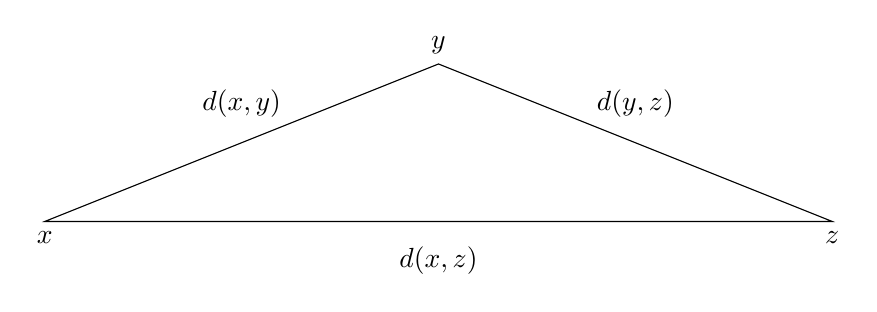
\begin{tikzpicture}
			\draw (0,0) node[anchor=north]{$x$}
			-- (10,0) node[anchor=north]{$z$}
			-- (5,2) node[anchor=south]{$y$}
			-- cycle;
			\draw (5,-0.5) node {$ d(x,z) $};
			\draw (2.5,1.5) node {$ d(x,y) $};
			\draw (7.5,1.5) node {$ d(y,z) $};
		\end{tikzpicture}
		\caption{The triangle inequality.}
	\end{figure}  
	Geometrically, this is equivalent to saying that the length of any side of a triangle cannot be greater than the sum of the other two lengths. Whenever presented with a weak inequality, it is often helpful to ask ``when does this hold with equality''? In this case the answer is when $ y $ is on the line segment formed by $ x $ and $ z $. In this case going to $ y $ isn't a detour at all, but just a trivial stop on the way from $ x $ to $ z $! 
	\begin{example}[Euclidean Metric]
		The real line $ \R $ is a metric space when equipped with the metric $ d(x,y)=|x-y| $. 
	\end{example}
	\begin{example}[Euclidean Metric]
		Euclidean space $ \R^n $ is a metric space when equipped with the metric $$ d(\mathbf{x},\mathbf{y})=|\x-\y|=\sqrt{(x_1-y_1)^2+\cdots+(x_n-y_n)^2} .$$  The Euclidean metric is intimately linked to the concept of a \textit{\color{red}norm}. Recall from linear algebra that Euclidean space is a vector space where vectors are elements of $ \R^n $, and scalers are elements of $ \R $. This space is equipped with function $ \norm{\cdot}_2:\R^n\to\R $ that measures the length of vectors. $$ \norm{\x}_2=\sqrt{x_1^2+\cdots+x_n^2}$$ We can write the Euclidean metric as $ d(\x,\y)=\norm{\x-\y}_2 $. Right now, don't worry too much about norms.\footnote{I admittedly am not certain of when it is best to introduce the concept of a norm. I don't like how \cite{rudin1964principles} talks about it in passing in when reviewing Euclidean space. Introducing it latter on when covering functional analysis is also problematic, because we're going to use the $ \sup $-norm before that to measure the distance between two functions.} 
	\end{example}
	\begin{example}[Taxi-Cab Metric]
		If our set is $ \R^2 $ we can let $ d(\mathbf{x},\mathbf{y})=|x_1-y_1|+|x_2-y_2| $. This is often referred to as the taxi-cab metric, as it is how you would measure distance if driving a car on a grid. We can extend to $ \R^n $ and let $ d(\mathbf{x},\mathbf{y})=\sum_{i=1}^{n}|x_i-y_i| $. 
	\end{example}
	\begin{example}[$ p $-Adic Metric]
		The previous examples are easy to verify, but this may not always be the case. Suppose are set is $ \Z $ and $ d:\Z\times\Z\to[0,\infty] $ is defined as $$ d(x,y)=\begin{cases}
			0\text{ if }x=y\\p^{-\max\{m\in\N|\ p^m|(x-y) \}}\text{ otherwise}
		\end{cases}$$ for some prime number $ p $. Before we verify this is a metric, it's worth getting a feel for how the metric actually works. If $ x\neq y $, then the distance between two points is $ p $ raised to some negative power. That negative power is defined to be the maximum whole number $ m $ such that $ (x-y) $ is divisble by $ p^m $. This gives us the vague idea that distance between points $ x $ and $ y $ is somehow related to how many times $ p $ shows up in the prime factorization of $ (x-y) $ (where $ m $ is the number of times). Let's take $ p=3 $, and pick several points in $ \Z $ to measure the distance between.    
		\begin{center}
			\begin{tabular}{cccccc}
				$ x $ & $ y $ & $ x-y $ & prime factorization of $ x-y $ & $ m $ & $ p^{-m} $ \\ \hline
				$ 100 $& 19  &  $ 81 $   &          $ 3^4 $                  &  $ 4 $  &     $ 1/81 $                  \\
				$ 368 $	& 8  &  $ 360 $   &            $ 2^3\cdot5\cdot9 $                &  $ 0 $  &  $ 1 $                     \\
				$ 35 $	& $ 5 $  &  $ 30 $   &  $ 2\cdot 3\cdot 5 $                           &      $ 1 $ & $ 1/3 $                 
			\end{tabular}
		\end{center}
		It turns out that the more factors of $ p $ that go into the prime factorization of $ (x-y)$, the closer $ x $ and $ y $ are. Furthermore, the maximum distance between any two points is $ 1 $, as $ p^0=1 $ for all $ p $. We will now verify that this is indeed a metric. 
		\begin{enumerate}
			\item The function $ d(x,y) $ is defined such that $ d(x,y)=0 $ if and only if $ x=y $. 
			\item We have $ (x-y)=-(y-x) $. Therefore, the prime factorization of each number differ only in sign, and give the same value $ m $. This implies that $ d(x,y)=d(y,x) $.  
			\item Note that to show $ d(x,z)\le d(x,y)+d(y,z) $ for all points in $ \Z $, it suffices to show that $ d(x,z)\le\max\{d(x,y),d(y,z)\} $. This inequality happens to be a stronger condition that implies the triangle inequality. Suppose $ p^m\mid(x-y) $ and $ p^n\mid(y-z) $. For some $ s,r\in\Z $, we having
			\begin{align*}
				x-y=p^mr\\y-z=p^ns.
			\end{align*}
			We can combine these equations to conclude $$x-z=(x-y)+(y-z)=p^mr+p^ns. $$ If $ m>n $, then $ x-z=p^n(p^{m-n}r+s)$ and $ d(x,z)=d(y,z) $. Similarly, if $ n>m $, $ d(x,z)=d(x,y) $. Finally if $ n=m $, then $$x-z=p^n(r+s)=p^m(r+s), $$ and $ d(x,z)=d(x,y)=d(y,z) $. These three cases gives the desired inequality. 
		\end{enumerate}
	\end{example}
	\begin{definition}\label{def}
		Let $ X $ be a metric space. A set $ E\subseteq X $ is \textit{\color{red} bounded} if there is a positive number $ M\in\R $ and a point $ x\in X $ such that $ d(x,y)<M $ for all $ x\in E $. If a set is no bounded, we say it is \textit{\color{red}unbounded}. 
	\end{definition}
	Boundedness insures that a set doesn't ``go off to infinity''. 
	\begin{example}
		The sets $ \N $, $ \Z $, $ \Q $, and $ \R $ are all unbounded. 
	\end{example}
	\begin{example}
		Both the intervals $ [a,b] $ and $ (a,b) $ are bounded in $ \R $. For any $ x,y\in[a,b] $, $ d(x,y)<d(a,b)+1 $. The same holds for $ (a,b) $. 
	\end{example}
	The metric space we are most interested in is of course $ \R^n $ equipped with the familiar Euclidean metric. We can use this metric to define the notion of an open or closed ball in $ \R^n $. 
	\begin{definition}\label{def}
		If $ \x\in\R^n $ and $ r>0 $, the \textit{\color{red} open ball} with center $ \x $ and radius $ r $ is defined as $$ B_r(\x)=\{\y\in\R^n\mid|\y-\x|<r\}. $$ 
	\end{definition} 
	\begin{definition}\label{def}
		If $ \x\in\R^n $ and $ r>0 $, the \textit{\color{red} closed ball} with center $ \x $ and radius $ r $ is defined as $$ \bar{B}_r(\x)=\{\y\in\R^n\mid|\y-\x|\le r\}. $$ 
	\end{definition}
	Open and closed balls in $ \R^n $ are a generalization of the open and closed intervals you were first introduced to in high school, and Figure 9 provides an illustration in $ \R^2 $. 
	\begin{figure}[h!]
		\centering
		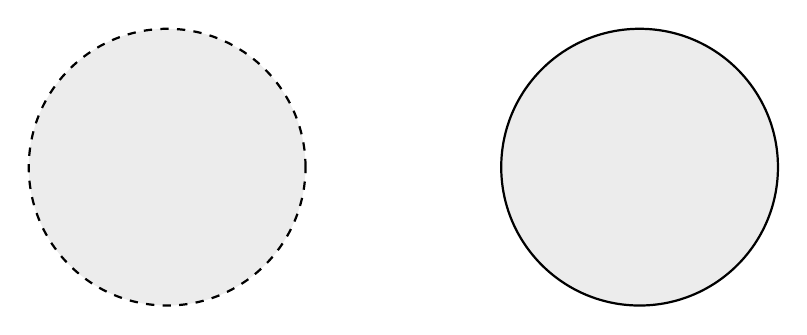
\begin{tikzpicture}
			\filldraw[color=black, fill=gray!15, thick, dashed] (0,0) circle (50pt);
			\filldraw[color=black, fill=gray!15, thick ] (6,0) circle (50pt);
		\end{tikzpicture}
		\caption{Open and closed balls in $ \R^2 $.}
	\end{figure}  
	\subsection{Open Sets, Closed Sets, and Boundaries}
	We want to generalize the notion of open and closed balls in $ \R^n $ to any metric space. In order to do these, we'll need to outline a couple preliminary definitions that classify the elements of a metric space. 
	\begin{definition}\label{def}
		A \textit{\color{red}neighborhood } of $ x $ in a metric space $ X $ is defined as $ N_r(x)=\{y\in X\mid d(x,y)<r\} $ for a radius $ r>0 $.\footnote{This definition is actually not quite correct for some reasons a bit more abstract than our setting at the moment. We'll come back to this in Example 13.2. I'm presenting it this way in an effort to follow \cite{rudin1964principles}.}   
	\end{definition}
	As the name implies, a neighborhood centered at $ x $ is simply all the points ``around'' $ x $. A neighborhood is its own set, and we will use them constantly. They are sort of like ``sets of utility'', because we will use them as tools to analyze the properties of other sets. If there is a set $ E $ in a metric space $ X $, we can use neighborhoods in $ X $ to learn about the points in $ E $. Are some neighborhoods subsets of $ E $? Do some neighborhoods intersect $ E $? Will the answers to these questions change if we make $ r $ really big or really small? It is worth thinking about these questions taking $ E $ to be one of the balls defined in Definition 3.3. Do the answers change if $ E $ is an open ball versus a closed ball? 
	
	Much like the open ball of Definition 3.2, neighborhoods do not include the points that are exactly a distance of $ r $ away from the point $ x $. In fact, if our metric space is $ \R^n $ with the standard metric, a neighborhood and open ball are precisely the same. 
	\begin{example}
		Let our metric space be $ \Z^2 $ equipped with the taxi-cab metric. Figure 10 shows the neighborhood centered at the origin of radius 3. 
		\begin{figure}[h]
			\centering
			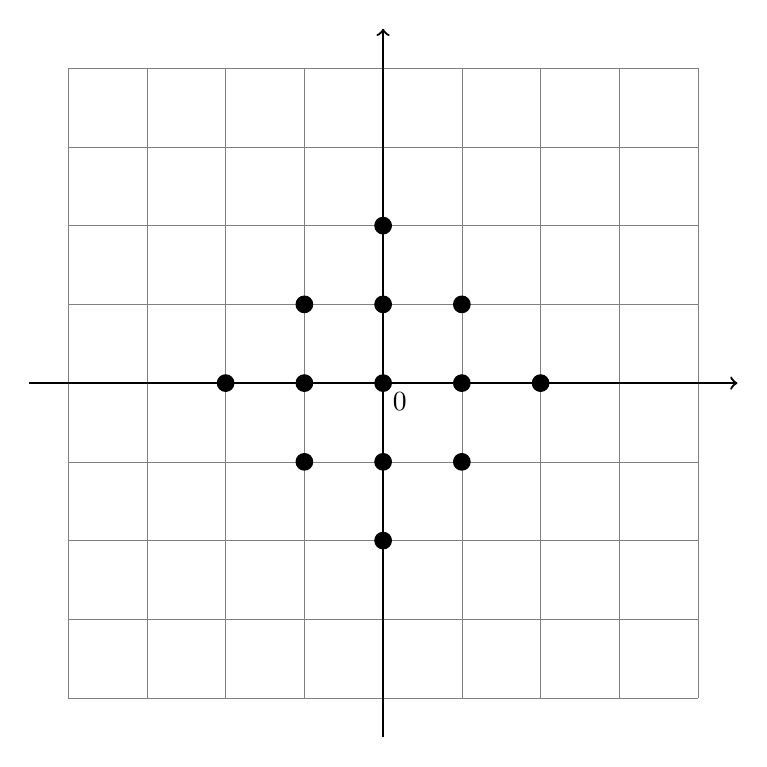
\begin{tikzpicture}
				\draw[step=1cm,gray,very thin] (-2,-2) grid (6,6);
				\draw[thick,->] (2,-2.5) -- (2,6.5);
				\draw[thick,->] (-2.5,2) -- (6.5,2);
				\filldraw (2,2) circle (3pt) node[anchor=north west] {$ 0 $};
				\filldraw (2,3) circle (3pt);
				\filldraw (2,4) circle (3pt);
				\filldraw (2,1) circle (3pt);
				\filldraw (2,0) circle (3pt);
				\filldraw (1,2) circle (3pt);
				\filldraw (1,3) circle (3pt);
				
				\filldraw (1,1) circle (3pt);
				
				\filldraw (0,2) circle (3pt);
				
				\filldraw (3,2) circle (3pt);
				\filldraw (3,3) circle (3pt);
				\filldraw (3,1) circle (3pt);
				
				\filldraw (4,2) circle (3pt);
				
				
			\end{tikzpicture}
			\caption{The set $ N_{3}(\mathbf{0})=\{\y\in\Z^2\mid|y_1|+|y_2|<3 \} $.}
		\end{figure}
	\end{example} 
	
	\begin{example}
		Let $ d_{2}:\R^2\times\R^2\to[0,\infty] $ be the euclidean metric, and $ d_{\ell^1}:\R^2\times\R^2\to[0,\infty] $ be the taxi-cab metric. A neighborhood in $ (\R^2, d_{1}) $ may have a different ``shape'' then it would in $ (\R^2, d_{2}) $. We will denote $ N_{3}(\mathbf{0})\in \R^2 $ as $ E $ and $ F $, in $ (X,d_{2}) $ and $ (X,d_{1}) $ respectively. These neighborhoods are shown in Figure 11.     
		\begin{figure}[h!]
			\centering
			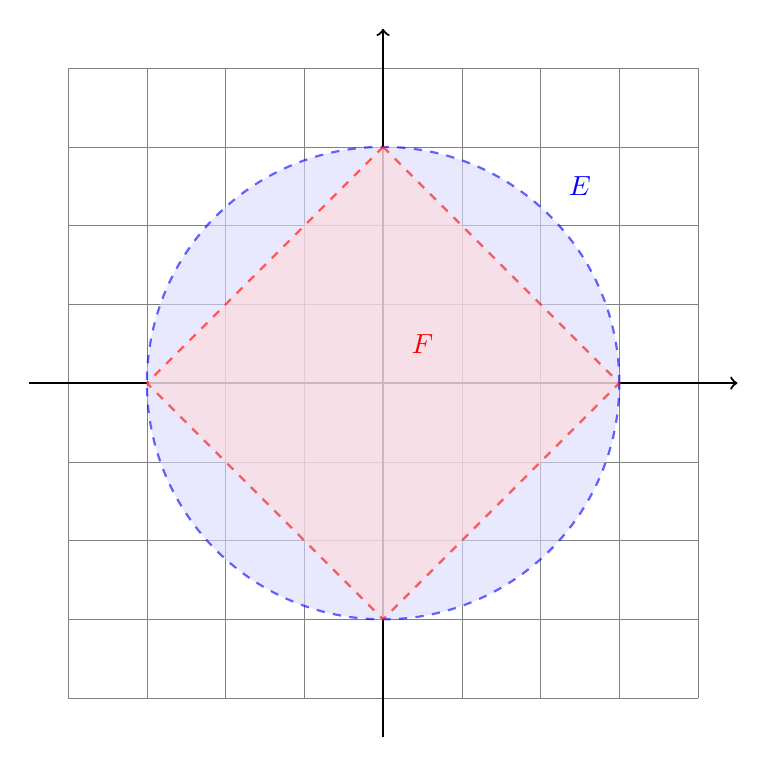
\begin{tikzpicture}
				\draw[step=1cm,gray,very thin] (-2,-2) grid (6,6);
				\draw[thick,->] (2,-2.5) -- (2,6.5);
				\draw[thick,->] (-2.5,2) -- (6.5,2);
				\filldraw[color=blue, fill=blue!15, thick, dashed, opacity=0.6] (2,2) circle (3cm);
				\filldraw[color=red, fill=red!15, thick, dashed, opacity=0.6] (2,5) -- (5,2) -- (2,-1) -- (-1,2) --(2,5) ;
				\draw[color = red] (2.5,2.5) node {$ F $};
				\draw[color = blue] (4.5,4.5) node {$ E $};
			\end{tikzpicture}
			\caption{$ N_{3}(\mathbf{0})\in \R^2 $ in $ (\R^2, d_{2}) $ and $ (\R^2, d_{1}) $. }
		\end{figure}	
	\end{example}
	\begin{definition}\label{def}
		Let $ X $ be a metric space. A point $ x\in X $ is a \textit{\color{red}limit point} of the set $ E\subseteq X $ if \textit{every} neighborhood of $ x $ contains a point $ y\in E $, where $ y\neq x $. We will denote the \textit{\color{red} set of all limit points} of $ E $ as $ E'=\{x\in X\mid x\text{ is a limit point of }E \}=\{x\in X\mid \in (N_r(x)\cap E)\backslash\{x\}\neq\emptyset\ \forall r>0\} $.
	\end{definition}
	\begin{note}
		For the remainder of Section 2, we will use $ X $ to denote a metric space, and $ E $ as some subset of $ X $. 
	\end{note}
	A limit point of a set is in some sense always ``close'' to points of the set. If $ x $ is a limit point of $ E\subseteq X $, then $ N_r(x) $ will always include points other than $ x $, no matter what we take $ r $ to be! We could make $ r $ smaller and smaller, but the set $ N_r(x) $ will never just be $ x $. In this sense, a limit point can always be ``approximated'' by elements in $ E $.  
	\begin{remark}
		Definition $ 3.5 $ never specifically said that a limit point of some set belongs to the set. As the next example shows, being a limit point has nothing to do with whether or not a point is included in the set in question. 	
	\end{remark}
	\begin{example}
		$\R^2$ is a good starting place. Suppose we have a set $ E\subseteq \R $ that for the most part forms a rectangle. The ``border'' of the rectangle is no included in $ E $. Also note that $ E $ includes an ``isolated'' point $ z $ (see Figure 12). Let's consider three points in $ \R^2 $: $ x $, $ y $, and $ z $.  
		\begin{figure}[h]
			\centering
			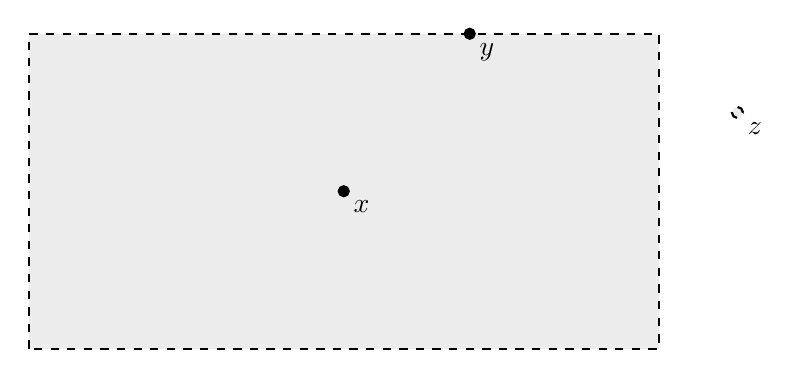
\begin{tikzpicture}
				\filldraw[color=black, fill=gray!15, thick, dashed] (0,0) rectangle (8,4);
				\filldraw (4,2) circle (2pt)node[anchor=north west] {$ x $};
				\filldraw (5.6,4) circle (2pt)node[anchor=north west] {$ y $};
				\filldraw[color=black, fill=gray!15, thick, dashed] (9,3) circle (2pt)node[anchor=north west] {$ z $};
			\end{tikzpicture}
			\caption{The set $ E\subseteq \R^2 $.}
		\end{figure}
		
		The point $ x $ belongs to $ E $. Furthermore, no matter what we take $ r $ to be, $ N_r(x) $ will never become a singleton of just $ \{x\} $. For the sake or argument, suppose $ x=(2,2) $. If $ r=0.5 $, then $ (2,2.49)\in N_{0.5}(x) $. Of $ r=0.01 $, then we still have $ (2,2.001)\in N_{0.01}(x) $. In fact, for every $ r $, we have $ (2,2+r/2)\in N_r(x) $. This means that $ x $ is a limit point of $ E $. 
		
		Now consider $ y $. This point does not belong to $ E $, but it is still a limit point! We could repeat the same argument we made for $ x $ without running into trouble, because every neighborhood of $ y $ will include points ``just below'' $ y $, all of which are in $ E $! What matters with limit points is not what set the point belongs to, but what set the points nearby it belong to. 
		
		Lastly, the point $ z $ is not a limit point. If we took $ r $ to be sufficiently large, then $ N_r(z) $ would include points in $ E $ that form the rectangle. Unfortunately, we could easily take $ r$ to be so small that $ N_r(z)=\{z\} $. It only takes one such $ r $ to rule out the chance of $ z $ being a limit point. We can provide a definition that corresponds to points like $ z $.     
	\end{example}
	
	\begin{definition}\label{def}
		Let $ X $ be a metric space. For a set $ E\subseteq X $, $ x\in E $ is an \textit{\color{red}isolated point} if it is not a limit point. That is, there exists an $ r>0 $ such that $ N_r(x)=\{x\} $. 
	\end{definition}
	By the definition of an isolated point, it is the opposite of a limit point, rendering the two definitions mutually exclusive. This definition also means any point $ x\in X $ is \textit{either} a limit point \textit{or} an isolated point.  An isolated point of any set is also included in the set, which is not the case for limit points. 
	\begin{definition}\label{def}
		Let $ X $ be a metric space. A point $ x\in X$ is an \textit{\color{red}interior point} of $ E\subseteq X $ if there exists \textit{a single} $ r>0 $ such that $ N_r(x)\subseteq E $. 
	\end{definition}
	\begin{example}
		Again, let's look at an example in $ \R^2 $. Let $ E\subseteq \R^2 $ be a closed ball that is ``punctured'' at $ z\in\R^2 $ such that $ z\notin E$. This can be seen in figure 13. The point $ x $ is in an interior point, as we could find some small $ r $ for which $ N_r(x)\subseteq E $. The point $ y $ is not an interior point of $ E $, because every single $ N_r(y) $ will contain some point outside of $ E $, meaning $ N_r(y)\not\subseteq E $. Finally, the point $ z $ is not an interior point, as each neighborhood of $ N_r(z) $ contains $ z $, and $ z\notin\ E $. Even though we can make $ r $ small enough to guarantee the only point in $ N_r(z) $ which is not in $ E $ is $ z $ $ (N_r(z)\backslash E=\{z\}) $, this point is all it takes to guarantee $ N_r(z)\not\subseteq E $ for all $ r $. 
		\begin{figure}[h]
			\centering
			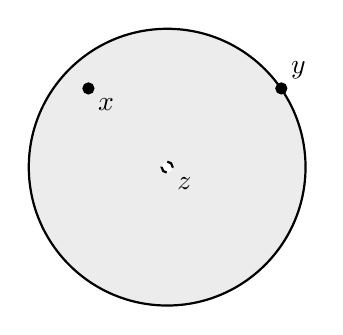
\begin{tikzpicture}
				
				\filldraw[color=black, fill=gray!15, thick ] (6,0) circle (50pt);
				\filldraw[color=black, fill=white, thick, dashed] (6,0) circle (2pt)node[anchor=north west] {$ z $};
				\filldraw (5,1) circle (2pt)node[anchor=north west] {$ x $};
				\filldraw (7.45,1) circle (2pt)node[anchor=south west] {$ y $};
			\end{tikzpicture}
			\caption{The set $ E\subseteq \R^2 $.}
		\end{figure}	
	\end{example}
	\begin{remark}
		While a limit point of $ E\subseteq X $ need not be a point in $ E $, an interior point of $ E $ must be an element of $ E $. If $ x $ is an interior point, then $ x\in N_r(x)\subseteq E $ for some $ r $, so $ x\in E $. 
	\end{remark}
	\begin{example}
		It may be tempting to conclude that an interior point must be a limit point, after all, if we can find an $ N_r(x)\subseteq E $, then it is likely each neighborhood would contain infinite points of $ X $. This logic makes the dangerous assumption that $ X $ is in infinite, and $ d(x,y) $ ``behaves like'' the Euclidean metric. Consider a metric space $ X $ with the discrete metric $$ d(x,y)=\begin{cases}
			1\text{ if }x\neq y\\
			0\text{ if }x=y
		\end{cases}.$$ 
		For any $ x\in X $, $ N_{1/2}(x)=\{x\}\subseteq X $. We have that $ x $ is an interior point, but not a limit point. 
	\end{example}
	We now briefly introduce the idea of an exterior point. The only difference between the  definition of an interior point and exterior point, will be that the neighborhood of a point will be in the complement of $ E $ for an exterior point. This small change in language will make a big difference in meaning. 
	\begin{definition}\label{def}
		Let $ X $ be a metric space. A point $ x\in X$ is an \textit{\color{red}exterior point} of $ E\subseteq X $ if there exists \textit{a single} $ r>0 $ such that $ N_r(x)\subseteq E^c $.
	\end{definition}
	\begin{remark}
		Any point $ x\in X $ is \textit{either} an interior point \textit{or} an exterior point.
	\end{remark}
	\begin{example}
		Let $ [0,1]\in \R $. The point $ 2\in\R $ is an exterior point of $ [0,1] $. 
	\end{example} 
	\begin{remark}[VERY IMPORTANT THEME]
		Nearly every definition in this section specifies a metric space $ X $. This means the metric space we work in could affect how we classify a point (and later sets). If we have two metric spaces $ X $ and $ Y $ where $ X\subseteq Y $, a point $ x\in E\subseteq X $ may be a limit point/interior point/exterior point in $ X $ but not in $ Y $. 
		
		We will see this come up again, and again. How a set/point behaves or is classified is contingent on what space we are in. A small change, whether it be the inclusion of some additional points, or changing the metric, can make a big difference. This means it is important to specify what space we're in if it is ever unclear. On the bright side, this all makes for great examples!   
	\end{remark}
	\begin{example}
		The set $ \R $ has no limit points when equipped with the discrete metric $$ d(x,y)=\begin{cases}
			1\text{ if }x\neq y\\
			0\text{ if }x=y
		\end{cases}.$$  
		
	\end{example}
	
	We already generalized the idea of some open or closed interval in $ \R $ to the concept of an open or closed ball in $ \R^n $. Now we will go one step further, by bringing these concepts to any metric space. 
	\begin{definition}\label{def}
		Let $ X $ be a metric space. A set $ E\subseteq X $ is \textit{\color{red}open} if every point of $ E $ is an interior point.  
	\end{definition}
	\begin{definition}\label{def}
		Let $ X $ be a metric space. A set $ E\subseteq X $ is \textit{\color{red}closed} if it contains all its limit points. That is, $ E'\subseteq E $. 
	\end{definition}
	\begin{example}
		Let $ (a,b)\subseteq\R $. This set is open, as for all $ x\in(a,b) $, we can find an $ r $ such that $ N_r(x)\subseteq(a,b) $. If $ d(a,x)\ge d(x,b) $, let $ r=d(x,b)/2 $. If $ d(x,b)>d(a,x) $ let $ r=d(x,a)/2 $.  Figure 14 shows this neighborhood for $ x $ where $ d(a,x)\ge d(b,x) $.
		\begin{figure}[h]
			\centering
			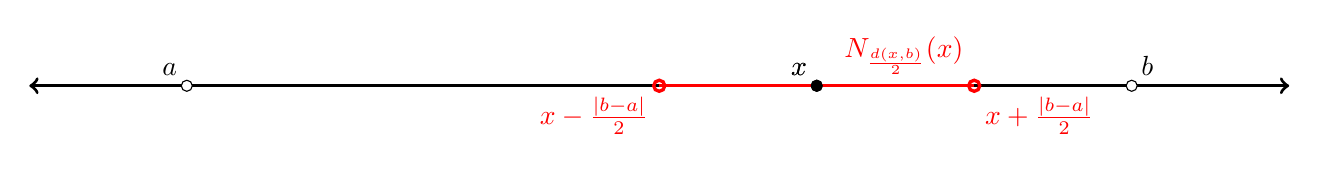
\begin{tikzpicture}
				\draw[very thick, color=red] (0,0) -- (2,0); 
				\draw[very thick, ->] (6,0) -- (8,0);
				\draw[very thick, ->] (-6,0) -- (-8,0);
				\draw[very thick] (-6,0) -- (6,0);
				\filldraw[fill=white] (-6,0) circle (2pt)node[anchor=south east] {$ a $};
				\filldraw[fill=white] (6,0) circle (2pt)node[anchor=south west] {$ b $};
				\filldraw[fill=black] (2,0) circle (2pt)node[anchor=south east] {$ x $};
				\draw[color=red, very thick] (4,0) circle (2pt)node[anchor=north west] {$ x+\frac{|b-a|}{2} $};
				\draw[color=red, very thick] (0,0) circle (2pt)node[anchor=north east] {$ x-\frac{|b-a|}{2} $};
				\draw[very thick, color=red] (0,0) -- (4,0) node[anchor=south east] {$ N_{\frac{d(x,b)}{2}}(x) $}; 
				\filldraw[fill=black] (2,0) circle (2pt)node[anchor=south east] {$ x $};
			\end{tikzpicture}
			\caption{The open interval $ (a,b)\subseteq \R $.}
		\end{figure}
		By construction, our neighborhood will always be a proper subset of $ (a,b) $, so each point of $ x $ is an interior point. Therefore $ (a,b) $ is open. On the other hand, $ (a,b) $ is not closed, because $ a $ and $ b $ are limit points, but neither are in the set $ (a,b) $.
	\end{example}
	\begin{example}
		Let $ [a,b]\subseteq\R $. This set is not open, as $ a $ and $ b $ are not interior points. For instance, $ a-r/2\in N_r(a) $ for all $ r>0 $. The number $ a-r/2\notin[a,b] $, so $ N_r(a)\not\subseteq[a,b] $ for all $ r $. While $ [a,b] $ is not open, it is closed. Every point in $ [a,b] $ is a limit point because $ \R $ is complete. The interval $ [a,b] $ trivially contains itself, so it contains all its limit points and is closed. 
	\end{example}
	\begin{example}
		Let $ X $ be a metric space, and $ E\subseteq X $. Any set with no limit points, $ E'=\emptyset $, is closed, because $ \emptyset\subseteq E $. This means any finite set is closed, as no finite set has limit points. Let $ X=\{x_1,\ldots, x_n\} $, and $ E\subseteq X $. If we let $ y\in E $, and set $ r=\min_{x\in X}d(x,y) $, then $ N_r(y)=\{y\} $. This means $ y $ fails to be a limit point for all $ y\in E $.
	\end{example}
	\begin{remark}
		The definitions of open and closed sets never imply that a set is either closed or open. It is possible for a set to be both closed and open, or be neither closed nor open.
	\end{remark}
	\begin{example}
		The set $ \emptyset $ in any metric space $ X $ is closed and open. This set has no limit points $ (\emptyset'=\emptyset) $, and $ \emptyset\subseteq\emptyset $, so it is closed. The set also has no points, so every point is an interior point, making $ \emptyset $ open. 
	\end{example}
	\begin{example}
		The set of rationals $ \Q $ is neither open nor closed in $ \R $. For all $ x\in\Q $, $ N_r(x) $ will contain irrational numbers for all $ r $, meaning $ N_r(x)\not\subseteq\Q $. Therefore no elements of $ \Q $ are interior points. The set $ \Q $ also does not contain all of its limit points, as any irrational number is a limit point as a result of Theorem 2.4. For example, any neighborhood of $ \sqrt{2} $ will contain elements of $ \Q $ (which are not $ \sqrt{2} $), making it a limit point. 
	\end{example}
	\begin{remark}[Relative to Which Space]
		The point made in Remark 2.4 is especially relevant for open and closed sets. A set could be open in one metric space, but closed in another. For example, if we have the space of real numbers $ [0,1] $ with the Euclidean metric, $ [0,0.5) $ is open in $ Y $. We also have that $ [0,1] $ is open in $ Y $! In most cases it's clear what metric space we are working in, but sometimes it is not. In cases where it is vague, it's always best to say a set is \textit{open in $ X $} or \textit{closed in $ X $}. For this reason it is a good practice to either specify $ E\subseteq X $, or include ``in $ X $.'' Many topics in analysis concern the metric space $ \R^n $ or $ \R $, so if you say a set is closed or open in conversation, it is usually assumed the metric space is one of these spaces. For example, if you were to ask someone ``are the integers closed or open?", they would most likely assume you mean ``are the integers closed or open in $ \R $?" 
	\end{remark}
	
	\begin{example}
		Suppose we want to determine if $ \Z $ is open or closed in $ \Z $. Every point is an interior point as $ N_{1/2}(x)={x}\subseteq\Z $ for all $ x\in\Z $, so $ \Z $ is open in $ \Z $. The set $ \Z $ has no limit points in $ \Z $, as $ N_{1/2}(x) $ does not include any points $ y\in\Z $ where $ y\neq x $. This gives that $ \Z'=\emptyset $,\footnote{This also means that every point of $ \Z $ is isolated.} so $ \Z\subseteq \Z' $, and $ \Z $ is closed in $ \Z $.
		
		Now let our metric space be $ \R $. Is $ \Z $ open in $ \R $? Let $ x\in\Z $. For any $ N_r(x) $ such that $ r<1 $, $ x-r/2\in N_r(x) $, where $ x-r/2\notin\Z $. If $ r\ge 1 $, then $ x-1/2\in N_r(x) $, where $ x-1/2\notin\Z $.\footnote{The case where $ r\ge 1 $ handles the situation where $ r/2\in\Z $. If this were the case, then $ x-r/2\in\Z $. This is not a problem, as $ N_r(x) $ would still contain an uncountably infinite number of reals numbers, but it makes explicitly finding one of those reals a little tricky. It's easier to just add or subtract $ 1/2 $ from $ x $ and call it a day.} Therefore, there exists no $ r $ such that $ N_r(x)\subseteq \Z $, so $ \Z $ is not open in $ \R $. We have that $ \Z $ is closed in $ \R $, as each point of $ \Z $ is still isolated.  
	\end{example}
	
	Before proving some useful properties of open and closed sets, there is one more definition that can prove helpful at times. It formalizes the notion of points in a set that are just on the border of a set, like the endpoints of $ [a,b]\subseteq\R $.  
	\begin{definition}\label{def}
		Let $ X $ be a metric space, and $ E\subseteq X $. The \textit{\color{red}boundary} of $ E $, denoted $ \partial E $, is the set of points in $ X $ such that every neighborhood of $ p $ contains at least one point of $ E $ and at least one point not of $ E $. $$ \partial E=\{x\in X\mid N_r(x)\cap E\neq\emptyset\text{ and }N_r(x)\cap  E^c\neq\emptyset \ \forall r>0  \} $$ 
		Any element of $ \partial E $ is a \textit{\color{red}boundary point}.
	\end{definition}
	There are several equivalent definitions of $ \partial E $, many of which are more popular than this specific one. These other definitions use terms that we will cover in Section 3.4, so we will circle back then and discuss the boundary of a again. The first example one's mind should jump to are open and closed balls in $ \R^n $. 
	\begin{figure}[h]
		\centering
		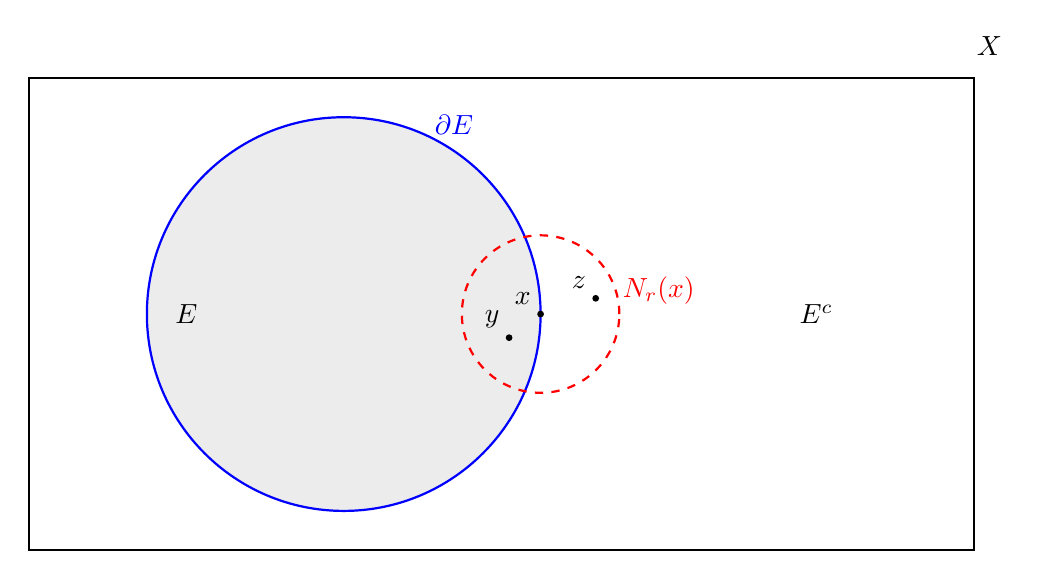
\begin{tikzpicture}
			\draw[color=black, thick ] (0,0) rectangle (12,6);
			\filldraw[color=blue, fill=gray!15, thick ] (4,3) circle (2.5cm);
			\draw (12.2,6.4) node {$ X $};
			\draw (2,3) node {$ E $};
			\draw (10,3) node {$ E^c $};
			\filldraw (6.1,2.7) circle (1pt) node[anchor = south east] {$ y $};
			\filldraw (6.5,3) circle (1pt) node[anchor = south east] {$ x $};
			\filldraw (7.2,3.2) circle (1pt) node[anchor = south east] {$ z $};
			\draw[color=red,dashed, thick ] (6.5,3) circle (1cm);
			\draw[color = red] (8,3.3) node {$ N_r(x) $};
			\draw[color = blue] (5.4,5.4) node {$ \partial E $};
		\end{tikzpicture}
		\caption{The boundary of a set $ E $ is shown in blue. Let $ \x\in X $. No matter how small we make $ r $, $ N_r(x) $ will always contain some $ y\in E $ and some $ z\in E^c $, so $ x\in\partial E $. } 
	\end{figure}
	\begin{example}
		Let $ B_r(\x) $ be the open ball of radius $ r $ centered at $ x\in\R^n $ (we could also denote this as $ N_r(\x) $). As the name suggests, the boundary is just all the points that are exactly a distance of $ r $ away from $ \x $, meaning $ \partial B_r(\x)=\{\y\in X\mid |\x-\y|=r\} $. In this particular case, no points in the boundary are in $ B_r(\x) $, so we have $ B_r(\x)\cap\partial B_r(\x)=\emptyset  $. If we take $ \bar{B}_r(\x) $ to be the closed ball, then we have the same boundary. $$\partial \bar{B}_r(\x)=\partial B_r(\x)=\{\y\in X\mid |\x-\y|=r\} $$ We also have $ \partial \bar{B}_r(\x)\cap \bar{B}_r(\x)=\bar{B}_r(\x)  $, and $ B_r(\x)\cup\partial B_r(\x)=\bar{B}_r(\x) $. 
	\end{example}
	\begin{remark}
		It is very tempting to think all boundary points are limit points. At first glance, the definition of a boundary point seems to imply a point $ x\in\partial E $ is not only a limit point of $ E $, but also a limit point of $ E^c $. This is not true! Suppose $ x\in E $ is a limit point. The definition of a limit point not only requires that $ N_r(x)\cap E $ for all $ r $, but also requires that there are points \textit{other than} $ x $ in $ N_r(x) $. A boundary point needn't satisfy this second requirement, so even if $ N_r(x)\cap E=\{x\} $ for all $ r $, $ x $ can still be a boundary point! 
	\end{remark}
	
	\begin{example}
		Let $ E\subseteq \R^2 $ be the union of a disk punctured at $ z $ and an isolated point $ y $ (Figure 16).  
		\begin{figure}[h]
			\centering
			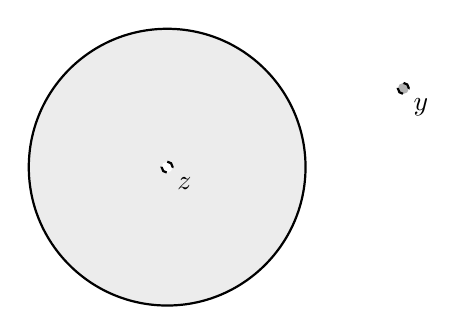
\begin{tikzpicture}
				\filldraw[color=black, fill=gray!15, thick ] (6,0) circle (50pt);
				\filldraw[color=black, fill=white, thick, dashed] (6,0) circle (2pt)node[anchor=north west] {$ z $};
				\filldraw[color=black, fill=gray!60, thick, dashed] (9,1) circle (2pt)node[anchor=north west] {$ y $};
			\end{tikzpicture}
			\caption{The set $ E\subseteq \R^2 $.}
		\end{figure}
		
		The points $ y $ and $ z $ are both boundary points. Despite this, $ y $ is not a limit point of $ E $, and $ z $ is not a limit point of $ E^c $. This follows from the reasoning in the previous remark.  	
	\end{example}
	
	\begin{remark}
		We have now introduced five different definitions that classify points: limit points, isolated points, interior points, boundary points, and exterior points. This is \textit{a lot} to take in all at once. By far the most important concepts introduced here were open and closed sets. Being able to determine if a set is open and/or closed is one of the most important skills to have for this section, and those that follow. 
	\end{remark}
	\subsection{Properties of Open and Closed Sets}
	Open set and closed sets will play a roll in many of the results and theorems to come, so it is important to be able to identify which sets are open and which are closed. We will know introduce several tools that make this easier.  
	\begin{proposition}
		Every neighborhood is an open set.
	\end{proposition}
	\begin{proof}
		Suppose we have a metric space $ X $, and some point $ x\in X $. We will show that any point $ y\in N_r(x) $ is an interior point. There exists some $ h $ such that $$d(x,y)=r-h .$$ I claim that $ N_{r'}(y)\subseteq E $ for $ r'<h $. For all points $ z $ such that $ d(y,z)=r'<h $, the triangle inequality gives $$d(x,z)\le d(x,y)+d(y,z)<r-h+h=r, $$ so $ z\in N_r(x)=E $ for all $ z $ by the definition of $ N_r(x) $. This implies that $ N_{r'}(y)\subseteq E $, making $ y $ an interior point. (Figure 17)
		\begin{figure}[h]
			\centering
			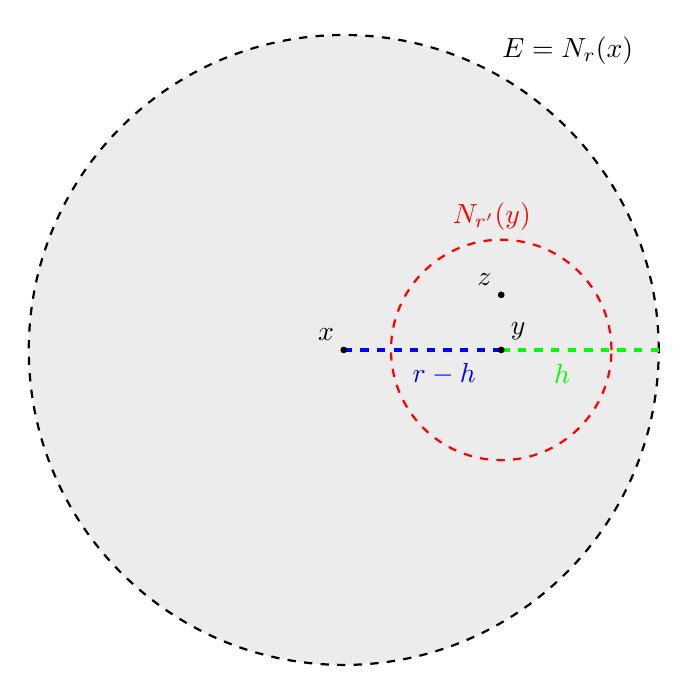
\begin{tikzpicture}
				\filldraw[color=black, fill=gray!15, thick, dashed ] (6,0) circle (4cm);
				\draw[very thick, dashed, color=blue] (6,0) -- (8,0);
				\draw[color=blue] (7.8,-0.3) node[anchor = east] {$ r-h $};
				\draw[very thick, dashed, color=green] (8,0) -- (10,0);
				\draw[color=green] (9,-0.3) node[anchor = east] {$ h $};
				\draw[color=black] (9.8,3.8) node[anchor = east] {$ E=N_r(x)$};
				\filldraw (6,0) circle (1pt) node[anchor = south east] {$ x $};
				\filldraw (8,0) circle (1pt) node[anchor = south west] {$ y $};
				\filldraw (8,0.7) circle (1pt) node[anchor = south east] {$ z $}; 
				\draw[color=red] (8.5,1.4)  node[anchor = south east] {$ N_{r'}(y) $};
				\draw[color=red, thick, dashed] (8,0) circle (1.4cm); 
			\end{tikzpicture}
			\caption{The set $ E\subseteq X $. We constructed a neighborhood $ N_{r'}(y) $ for an arbitrary $ y\in N_r(x) $ such that $ N_{r'}(y)\subseteq E $. }
		\end{figure}
	\end{proof}
	
	\begin{proposition}
		If $ x\in X $ is a limit point of $ E $ ($ x\in E' $), then every neighborhood of $ x $ contains infinitely many points of $ E $.
	\end{proposition}
	\begin{proof}
		Let $ x\in X $. Suppose for contradiction, there exists some $ N_r(x) $ which contains only a finite number of points of $ E $. Let this finite set of points be $ \{y_1, \ldots, y_n\}\subseteq N_r(x)\cap E $. Pick the radius of $ N_r(x) $ to be the distance between $ x $ and the point to which it is closest in the finite set $ \{y_1,\ldots,y_n\} $: $$ r=\min_{1\le m\le n} d(x,y_m). $$ By construction, $ N_r(x) $ contains no point $ y\in E $ such that $ y\neq x $, so $ x $ is not a limit point of $ E $. This is a contradiction. (Figure 18)
		\begin{figure}[h]
			\centering
			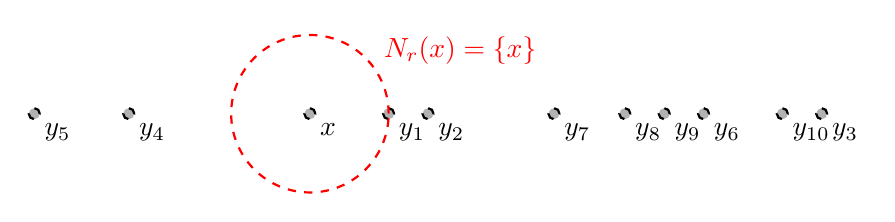
\begin{tikzpicture}
				\filldraw[color=black, fill=gray!60, thick, dashed] (1,0) circle (2pt)node[anchor=north west] {$ y_1 $};
				\filldraw[color=black, fill=gray!60, thick, dashed] (0,0) circle (2pt)node[anchor=north west] {$ x $};
				
				\filldraw[color=black, fill=gray!60, thick, dashed] (1.5,0) circle (2pt)node[anchor=north west] {$ y_2 $};
				\filldraw[color=black, fill=gray!60, thick, dashed] (6.5,0) circle (2pt)node[anchor=north west] {$ y_3 $};
				\filldraw[color=black, fill=gray!60, thick, dashed] (-2.3,0) circle (2pt)node[anchor=north west] {$ y_4 $};
				\filldraw[color=black, fill=gray!60, thick, dashed] (-3.5,0) circle (2pt)node[anchor=north west] {$ y_5 $};
				\filldraw[color=black, fill=gray!60, thick, dashed] (5,0) circle (2pt)node[anchor=north west] {$ y_6 $};
				\filldraw[color=black, fill=gray!60, thick, dashed] (3.1,0) circle (2pt)node[anchor=north west] {$ y_7 $};
				\filldraw[color=black, fill=gray!60, thick, dashed] (4,0) circle (2pt)node[anchor=north west] {$ y_8 $};
				\filldraw[color=black, fill=gray!60, thick, dashed] (4.5,0) circle (2pt)node[anchor=north west] {$ y_9 $};
				\filldraw[color=black, fill=gray!60, thick, dashed] (6,0) circle (2pt)node[anchor=north west] {$ y_{10} $};
				\draw[color=red, thick, dashed] (0,0) circle (1cm);
				\draw[color=red] (3,.5)  node[anchor = south east] {$ N_{r}(x)=\{x\} $};
			\end{tikzpicture}
			\caption{If our finite set of points of $ E $ is $ \{y_1,\ldots,y_{10}\} $, then we can reach a contradiction by constructing a neighborhood of $ x $ with $ r=\min_{1\le m\le n} d(x,y_m)=d(x,y_1) $. This will hold no matter where the points  $ \{y_1,\ldots,y_{10}\} $ happen to be in $ E $. In this case $ x\in E $, but remember that this isn't a requirement.}
		\end{figure}
	\end{proof}
	
	\begin{corollary}
		A finite set has no limit points. (see Example 3.13)
	\end{corollary}
	The next theorem and its corollary allows us to determine if a set is open or closed based on its complement. At first, this may not seem helpful, but if it is not clear if $ E $ is open or closed, one can just use $ E^c $! We will provide examples where using $ E^c $ is easier.
	\begin{theorem}
		A set $ E $ is open \textit{if and only if} its complement is closed.
	\end{theorem}
	\begin{proof}{\color{white}space}
		\begin{enumerate}
			\item [$ (\Longrightarrow) $] Suppose $ E $ is open. Let $ x\in X $ be a limit point of $ E^c $. Every neighborhood $ N_r(x) $ contains a point of $ E^c $, so $ N_r(x)\not\subseteq E $, meaning $ x $ is \textit{not} and interior point of $ E $. But we have assumed every point of $ E $ is an interior point, so $ x\in E^c $. Therefore $ E^c $ includes all its limit points and is closed.   
			\item [$ (\Longleftarrow) $] Suppose $ E^c $ is closed. Let $ x\in E $. We have $ x\notin E^c $, so $ x $ is not a limit point of $ E^c $ (otherwise it would be in $ E^c $, as $ E^c $ is closed). If $ x $ is not a limit point of, then there exists an $ N_r(x)\cap E^c=\emptyset $, giving $ N_r(x)\subseteq E $. Thus $ x\in E $ is an interior point, and $ E $ is open.  
		\end{enumerate}
	\end{proof}
	\begin{corollary}
		A set $ E $ is closed \textit{if and only if} its complement is open.
	\end{corollary}
	One practical consequence of these results, is that if you find it more difficult to check if a set is open or closed (or vice versa), you can always just work with the complement. 
	
	\begin{example}
		Let $ X $ be any metric space. Recall from Example 3.14 that $ \emptyset $ is closed and open. This means that $ \emptyset^c=X $ is closed and open as well. This allows us to conclude that $ \R $ in $ \R $ is open and closed.
	\end{example}
	\begin{example}
		The set $ [a,b]\subseteq \R $ is closed. This implies that $ [a,b]^c=(-\infty,a)\cup(b,\infty) $ is open.
	\end{example}
	We often define some set of interest as a union or intersection of a collection of sets. For instance, the proof of Theorem 1.2, the supremum of a set in $ \R $ was defined as the union of the Dedekind cuts that comprise the set. In Example 1.27, $ \Q $ was written as the countably infinite union of intervals. In situations like this, it is possible to know if a set is open or closed if the sets over which we take the union/intersection are open or closed. 
	\begin{theorem}
		Let $ \{G_\alpha\} $ and $ \{F_\alpha\} $ be an arbitrary collection of open sets and closed sets respectively. Let $ G_1,\ldots,G_n $ and $ F_1,\ldots, F_n $ be a finite collection of open sets and closed sets respectively. In this case we have:
		\begin{enumerate}
			\item $ \bigcup_\alpha G_\alpha $ is open.
			\item $ \bigcap_\alpha F_\alpha $ is closed.
			\item $ \bigcap_{i=1}^n G_i$ is open.
			\item $ \bigcup_{i=1}^n F_i$ is closed.
		\end{enumerate}
		
	\end{theorem}
	
	\begin{proof}{\color{white}space}
		\begin{enumerate}
			\item Suppose $ G_\alpha $ is open for all $ \alpha $. Let $ x\in \bigcup_\alpha G_\alpha $. For some $ \alpha $, $ x\in G_\alpha $. There exists a neighborhood $ N_r(x) $ such that $ N_r(x)\subseteq G_\alpha $, because $ G_\alpha $ is open. Therefore $ \bigcup_\alpha G_\alpha $ is open, as $ N_r(x)\subseteq G_\alpha\subseteq \bigcup_\alpha G_\alpha $. 
			\item Suppose $ F_\alpha $ is closed for all $ \alpha $. It suffices to show that $ (\bigcap_\alpha F_\alpha)^c $ is open using Theorem 2.1. By the aforementioned theorem, $ F_\alpha^c $ is closed for all $ \alpha $. Therefore the union of $ F_\alpha^c $ is open by part (1). This completes our proof, as De Morgan's Law gives $$ \left(\bigcap_\alpha F_\alpha\right)^c=\bigcap_\alpha F_\alpha^c.$$
			\item Suppose the sets $ G_1,\ldots,G_n $ are open. Let $ x\in \bigcap_{i=1}^n G_i$. For all $ x\in\bigcap_{i=1}^n G_i $, there exists neighborhoods $ N_{r_i}(x) $ with radii $ r_i $, such that $ N_{r_i}(x)\subseteq G_i $ for all $ i $. Let $ r=\min\{r_1,\ldots,r_n\} $. This radius gives us $ N_r(x)\subseteq G_i $ for all $ i $, meaning $ N_r(x)\subseteq \bigcap_{i=1}^n G_i $. Therefore $ x $ is an interior point, and $ \bigcap_{i=1}^n G_i $ is open. (Figure 19)   
			\begin{figure}[h!]
				\centering
				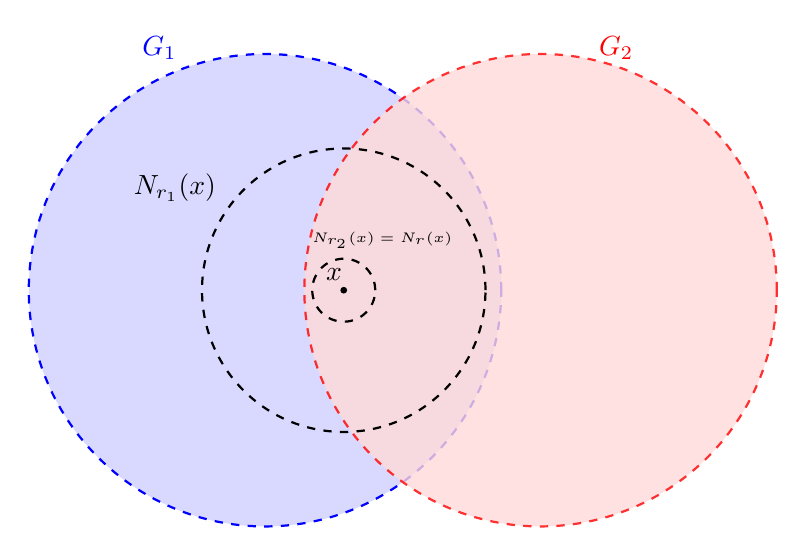
\begin{tikzpicture}
					\filldraw[color=blue, fill=blue!15, thick, dashed, opacity=1] (0,0) circle (3cm);\filldraw[color=red, fill=red!15, thick, dashed, opacity=0.8] (3.5,0) circle (3cm);
					\draw[color=blue] (-1,2.8)  node[anchor = south east] {$ G_1 $};
					\draw[color=red] (4.8,2.8)  node[anchor = south east] {$ G_2 $};
					\filldraw(1,0)  circle (1pt);
					\draw (1.1,0) node[anchor = south east] {$ x $};
					\draw[dashed, thick] (1,0) circle (1.8cm);
					\draw[dashed, thick] (1,0) circle (0.4cm);
					\draw(-0.5,1)  node[anchor = south east] {$ N_{r_1}(x) $};
					\draw(2.5,0.4)  node[anchor = south east] {\tiny$ N_{r_2}(x)=N_r(x) $};
				\end{tikzpicture}
				\caption{In this simplified setting, we have two open sets: $ G_1 $, and $ G_2 $. By letting $ r=\min\{r_1,r_2\}=r_2 $, we find a neighborhood $ N_r(x) $ such that $ N_r(x)\subseteq G_1\cap G_2 $. }
			\end{figure}
			\item  Suppose the sets $ F_1,\ldots,F_n $ are closed. It suffices to show that $ (\bigcap_{i=1}^n F_i)^c $ is open using Theorem 2.1. By the aforementioned theorem, $ F_i^c $ is open for all $ i$. By part (2) the the intersection of all $ F_i^c $ is open This complete out proof, as De Morgan's Law gives 
			$$ \left(\bigcap_{i=1}^n F_i\right)^c=\bigcap_{i=1}^n F_n^c.$$
		\end{enumerate}
	\end{proof}
	Part (2) and (4) of Theorem 2.2 require that the collection of sets is finite, otherwise the minimum over the finite number of radii of neighborhoods many not be well defined. The following two examples show that Theorem 2.2 does not hold if we take these collections to be infinite. 
	\begin{example}
		Let $ G_n=(1/n,1+1/n) $ for all $ n\in\N $. The set $ G_n $ is open in $ \R $ for all $ n $. Taking the intersection gives $$\bigcap_n G_n=[0,1] .$$ The interval $ [0,1] $ is closed, despite each $ G_n $ being open.  
	\end{example}
	\begin{example}
		Let $ F_n=[1/n,\infty) $ for all $ n\in\N $. The set $ F_n $ is closed in $ \R $ for all $ n $. Taking the union gives $$ \bigcup_{n}F_n=(0,\infty).$$ This interval is open in $ \R $, despited each $ F_n $ being closed.
	\end{example}
	\subsection{Closures, Interiors, Dense Sets, and Perfect Sets} 
	There are a handful of other definitions related to open set and closed sets that deserve a bit of attention.
	\begin{definition}\label{def}
		Let $ X $ be a metric space. The \textit{\color{red}interior} of a set $ E\subseteq X $, denoted $ E^\circ $, is the set of all interior points of $ E $. $$ E^\circ=\{x\in X\mid x\text{ is an interior point of }E \} $$
	\end{definition}
	The set $ E^\circ $ is clearly open, as by definition it is comprised only of interior points. Because interior points of $ E $ must be in $ E $, we have $ E^\circ \subseteq E $. Informally, we can think of $ E^\circ $ as the smallest open set contained within $ E $. This interpretation leads to the conclusion that if $ E $ is open, then $ E=E^\circ $.
	\begin{example}
		Let $ [a,b]\subseteq\R $. The interior of this set is $ (a,b) $. 
	\end{example}
	\begin{definition}\label{def}
		Let $ X $ be a metric space. The \textit{\color{red}closure} of a set $ E\subseteq X $ is $ \bar{E}=E\cup E' $. 
	\end{definition}
	The closure $ \bar{E} $ is the opposite of the interior in a certain sense. The closure can be though of as the smallest closed set that $ E $ is contained in. If $ E $ is closed, then $ E'\subseteq E $, and $ E=\bar{E} $.
	\begin{example}
		Let $ (a,b)\subseteq\R $. The closure of this set is $ [a,b] $. 
	\end{example}
	\begin{definition}\label{def}
		Let $ X $ be a metric space. The set $ E\subseteq X $ is \textit{\color{red}dense in $ X $} if every point of $ X $ is a limit point of $ E $, or a point of $ E $. ($ \bar{E}=X $)  
	\end{definition}
	
	Informally, if $ E $ is dense in $ X $, then we can approximate any point of $ X $ with a point in $ E $ arbitrarily well. This follow from the fact that any point in $ X $ is either in $ E $, or a limit point of $ E' $, or both.  We have already seen one example of this with Theorem 1.4.
	\begin{example}
		The set $ \Q $ is dense in $ \R $, that is $ \bar{\Q}=\R $. One implication of this fact is that the irrational numbers $ \R\backslash\Q $ are limit points of $ \Q $. We also have that the irrationals $ \R\backslash\Q $ are dense in $ \Q $!
	\end{example}
	Many results involving approximation can be stated in terms of dense sets. One of these is the Weierstrass Approximation Theorem. This will be formally treated and proved in Section 7, but for now we will give the result as an example of a dense set.
	\begin{example}[Weierstrass Approximation Theorem]
		Let $ C([a,b])=\{f\mid f:[a,b]\to \R\text{ and } f\text{ continuous}\} $ be the set of real valued continuous functions with domain $ [a,b] $. Now let $ \mathscr{P}([a,b]) $ be the set of all real valued polynomials with domain $ [a,b] $.\footnote{This set is traditionally denoted as $ \R[x] $ in abstract algebra.} The set $ \mathscr{P}([a,b])  $ is dense in $ C([a,b]) $. We will always be able to approximate a continuous function on a bounded interval arbitrarily well with polynomials. This result, and spaces of functions, will be discussed again in Section 7. 
	\end{example}
	\begin{definition}\label{def}
		Let $ X $ be a metric space. The set $ E\subseteq X $ is \textit{\color{red}perfect} if every point of $ E $ is a limit point of $ E $ $ (E=E') $. 
	\end{definition}
	If $ E $ is perfect, every point in $ E $ can be approximated arbitrarily well by other points in $ E $. 
	\begin{example}
		The real line $ \R $ is a perfect set. 
	\end{example}
	\subsection{Compact Sets}
	We have encountered infinity several times now. Sets can have an infinite number of element, in which case they are either countable or uncountable. A set can ``take up an infinite amount of space'' if it is unbounded. Each limit point of a set contains an infinite number of points in the set. These factors can result in sets that are difficult to work with. For example, suppose a set is unbounded. It can be hard to determine how functions or sequences behave on sets like this, because the distance between points can become arbitrarily large. What kind of headaches to limit points cause? Any neighborhood of a limit point will contain an infinite number of points in that set (Proposition 2.2). If the limit point is not in the set, this can also pose problems. As we will see later on, it could be possibly to get arbitrarily close to that limit point while never leaving the set. In a sense, we would be getting closer to a point in a set, where the destination is not even included in the set. To prevent this from happening, all limit points should be included in a set, i.e the set should be closed. Later on when working with sequences and continuous functions, two concepts intrinsically linked by the idea of getting arbitrarily close to a point, sets that are ``nice'', and will not illicit the two mentioned complications, will lead to nice results. Our goal now is to characterize these sets, and attempt to motivate their characterization.\footnote{Motivating the main definition of this subsection is infamously difficult, as it is not clear how it will be used in the future. It would be like explaining what a hammer is to someone who has no idea what a nail is. }   
	
	One somewhat trivial way to guarantee a set is both closed and bounded is by restricting out attention to finite sets. If $ E $ is finite, it has no limit points and is trivially closed. A finite set must also be bounded. While finite may have the nice properties we are looking for, they are not that interesting. Real analysis almost always involves the real numbers, an uncountably infinite set. So what criteria would guarentee an infinite set, whether it be countable or uncountable, will behave like a finite set?
	
	The way we will go about defining these sets is by looking how we can ``cover'' them with a collection of open sets. The idea is that a set may be infinite, but perhaps we can cover it with a finite collection of open sets. 
	\begin{definition}\label{def}
		Let $ X $ be a metric space. An \textit{\color{red}open cover} of a set $ E\subseteq X $ is a collection of open sets $ \mathcal\{G_\alpha\}\subseteq X $ such that $ E\subseteq\cup_\alpha G_\alpha $.  
	\end{definition}
	\begin{figure}[h]
		\centering
		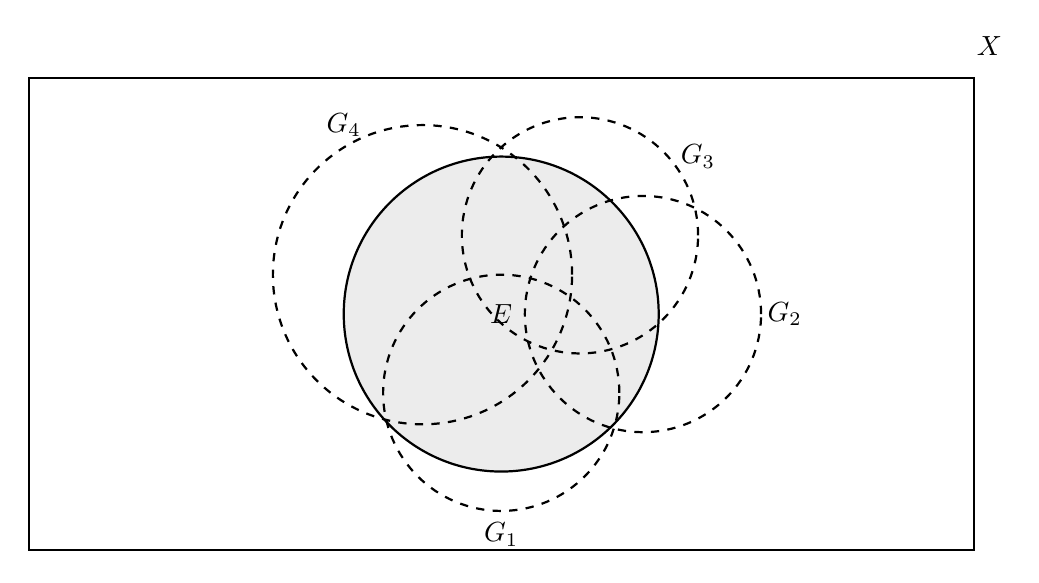
\begin{tikzpicture}
			\draw[color=black, thick] (0,0) rectangle (12,6);
			\filldraw[thick, fill=gray!15] (6,3) circle (2cm);
			\draw (12.2,6.4) node {$ X $};
			\draw (6,3) node {$ E $};
			\draw[thick, dashed] (6,2) circle (1.5cm);
			\draw (6,0.2) node {$ G_1 $};
			\draw[thick, dashed] (7.8,3) circle (1.5cm);
			\draw (9.6,3) node {$ G_2 $};
			\draw (8.5,5) node {$ G_3 $};
			\draw (4,5.4) node {$ G_4$};
			\draw[thick, dashed] (7,4) circle (1.5cm);
			\draw[thick, dashed] (5,3.5) circle (1.9cm);
		\end{tikzpicture}
		\caption{The collection of set $ \{G_1,\ldots G_4\} $ forms an open cover of $ E $.} 
	\end{figure}
	An open cover is a \textit{collection} of sets. Each element of an open cover is a single open set. This means that the cardinality of an open set has \textit{nothing} to do with the cardinality of the sets it is comprised of. The collection $ \{\R,(0,1),(0,2)\} $ is 3. We do not care whatsoever about the fact that each of the sets in the collection are uncountably infinite. The emphasis here is due to the fact that the cardinality of these covers (and a second type we will define soon) will be the bases of our criteria of what makes a set ``nice''.
	\begin{example}
		Let $ E=N_r(x) $ be a subset of a metric space $ X $. One open cover of the set $ E $ is the single set $ N_{r+1}(x) $. Another would be $ N_{r+2}(x) $. 
	\end{example}
	\begin{example}
		Let $ \R $ be the entire real line. We can cover this with the union of all sets of the form $G_n=(-n,n)$ for $ n\in\N $. $$ \R\subseteq\bigcup_{n\in \N}(-n,n)$$
	\end{example}
	It is not enough to require that a set has a finite open cover. Any set $ E $ can trivially be covered by itself, forming an open cover consisting of one element. We could require that every open cover is finite, but this could never be satisfied. For example, take the closed interval $ (a,b)\subseteq\R $. We could cover this with a finite open cover $ \{(a,b)\} $. We could also cover it with the infinite open cover $ \{(a,b),(-1,1),(-2,2),(-3,3),\ldots\} $. We can just take the cover $ \{(a,b)\} $ and throw in an infinite number of random intervals of $ \R $ and still end up with an open cover. This is complete ``overkill'' when it comes to covering $ (a,b) $! To address the fact that we will always have infinite open covers, we will introduce a new type of open cover that is both finite, and limits any redundant additions to the cover. 
	
	\begin{definition}\label{def}
		Let $ X $ be a metric space, and $ E\subseteq X $. A \textit{\color{red}finite subcover} of an open cover $ \{G_\alpha\} $ of $ E $  is a collection of open sets $ \{G_{\alpha_1},\ldots,G_{\alpha_n}\} $ such that $$ E\subseteq \bigcup_{i=1}^nG_{\alpha_i}\subseteq\bigcup_\alpha G_\alpha. $$
	\end{definition}
	\begin{example}
		Let $ X $ be a metric space and $ E\subseteq X $. The collection $ \{E\} $ is a trivial open cover. We also have a trivial finite open subcover in $ \{E\} $. 
	\end{example}
	\begin{example}
		Let $ \{(a,b),(-1,1),(-2,2),(-3,3),\ldots\} $ be an open cover of $ (a,b)\subseteq \R $. One finite subcover of this open cover is $ \{(a,b)\} $. Another finite subcover is $ \{(a,b),(-1,1)\} $. In fact, any set $ \{(a,b),(-1,1),\ldots(-n,n)\} $ is a finite subcover. 
	\end{example}
	This simple example shows that some open covers actually have an infinite number of finite subcovers. The introduction of finite subcovers may be a bit confusing, so it is worth recapping what we have done before presenting the main definition of this subsection: 
	\begin{itemize}
		\item We have some metric space $ X $ and some set $ E\subseteq X $. We can cover this set with a collection of sets $ \{G_\alpha\} $ called an open cover, the cardinality of which is determined by the number of sets in the collection $ \{G_\alpha\} $. We like the idea of finite open covers.
		\item There exists an infinite number of open covers of a set. There also always exists a finite open cover of a set, so we need to do better than just having a finite open cover.  
		\item A finite subcover $ \{G_{\alpha_1},\ldots,G_{\alpha_n}\} $ of the open cover $ \{G_\alpha\} $ is a subset of $ \{G_\alpha\} $, which also covers $ E $. The finite subcover of one open cover $ \{G_\alpha\} $ \textit{is not necessarily} a finite subcover of another open cover $ \{G'_\alpha\} $, so whenever we talk about finite subcovers, it is with respect to some fixed open cover. Some open covers of sets have an infinite number of finite subcovers (Example 2.29).
	\end{itemize} 
	We are now ready give a proper definition and name to the ``nice'' sets we want to characterize. In doing so, we will answer an important question about finite subcovers that may have arisen by now -- some open covers of sets have an infinite number of finite subcovers, but do \textit{all} open covers of a set have \textit{at least one} finite subcover? 
	\begin{definition}\label{def}
		Let $ X $ be a metric space, and $ K $ be a subset of $ X $. The set $ K $ is \textit{\color{red}compact} if \textit{every} open cover of $ K $ contains \textit{at least one} finite subcover. 
	\end{definition} 
	The answer to our question turns out to be no. If it were yes, then there would be no need to define compactness, because every set would be compact. Compact sets turn out to be the nice sets we were looking for. As we'll see, they can be infinite, but they do not cause the complications with infinity that we discussed at the open of this subsection. In some sense, compact sets are the next best thing to finite sets. 
	\begin{example}
		The set $ (a,b)\subseteq\R $ is not compact. In order verify this, we just need to find a single open cover that has no finite subcover. Let $ \{G_n\} $ be an open cover where $ G_n=(a+1/n,b) $. We have that $$ (a,b)\subseteq\bigcup_{n\in \N} G_n=\bigcup_{n\in \N}(a+1/n,b)=(a,b).$$ No finite subset of $ \{G_n\} $ will be a finite subcover of $ (a,b) $. If we had a finite subset of $ \{G_n\} $ then there would exist some $ N\in\N $ such that $ (a,a+1/N) $ is ``uncovered''. Therefore any open interval in $ \R $ is not compact. 
	\end{example}
	\begin{example}
		The real line $ \R $ is not compact. The open cover $ \{G_n\} $ where $ G_n=(-n,n) $ has no finite subcover. If we had a finite subset of $ \{G_n\} $, then there would exist some $ N\in\N $ such that $ (-\infty,-N)\cup(N,\infty) $ is ``uncovered''. Therefore the real line $ \R $ is not compact. 
	\end{example}
	
	These two examples should not be entirely surprising. When compactness was motivated, complications involving two types of sets were cited: unbounded sets, and sets that were not closed. $ (a,b) $ and $ \R $ both fall into exactly one of these categories.
	\begin{example}
		Suppose $ X=\{x_1,\ldots,x_n\} $ is a finite metric space. The entire space $ X $ is compact. Let $ \{G_\alpha\} $ be an open cover of $ X $. For each $ x_i\in X $, there exists an $ G_{\alpha_i} $ such that $ x_i\in G_{\alpha_i} $. Therefore, the open cover has a finite subcover in $ \{G_{\alpha_1},\ldots ,G_{\alpha_n}\} $.    
	\end{example}
	Using the definition of compactness to verify that a set is not compact takes some creativity, but only requires one to find a single counterexample. This is opposed to verifying a set is compact. This requires we somehow verify that every single open cover has a finite subcover. This is prohibitively difficult to do in most cases. This is why we want to find conditions that are easy to verify and that imply compactness. Of chief concern, is doing this for subsets of $ \R^n $. 
	\subsection{Properties of Compact Sets}
	Before restricting our attention to $ \R^n $, we need to establish some properties of compact sets that will allow come in handy when working with them. Unfortunately, we still do not have any nontrivial examples of compact sets, so some of these results will not have examples presented alongside them. Once we are able to identify compact sets in $ \R^n $ by means other then the definition of compactness, these results can be verified. 
	\begin{lemma}
		Suppose $ Y\subseteq X $. A subset $ E\subseteq Y$ is open in $ Y $ \textit{if and only if} $ E=Y\cap G $ for some open $ G\subseteq X $. 
	\end{lemma}
	\begin{proof}{\color{white}space}
		\begin{enumerate}
			\item[$ (\Longrightarrow) $] Suppose $ E\subseteq Y $ is open in $ Y $. For each $ x\in E $, there exists a $ r_x $ such that $ N_{r_x}(x)\subseteq E $. By the definition of a neighborhood, for all $ y\in Y $ satisfying $ d(x,y)<r_x $, we have $ y\in E $. Denote $ N_{r_x}(x)=V_x $ for all $ x\in E $, and define $$G=\bigcup_{x\in E}V_x .$$ The set $ G $ is a union of open sets, so it is open (Figure 21). I now claim that $ E=G\cap Y $, which is our desired result. For $ x\in E $, we have $ x\in V_x $ for all $ x\in X $, so $ x\in E $ and $ x\in Y $. This gives $ E\subseteq G\cap Y $. Now let $ x\in G\cap Y $. For the corresponding $ V_x $, $ V_x\cap Y\subseteq E $. This implies $ G\cap Y\subseteq E $.    
			\item[$ (\Longleftarrow) $] Suppose $ E=Y\cap G $ for some open $ G $ in $ X $. The set $ G $ is open, so for all $ x\in E $ there exists a neighborhood $ N_r(x)\subseteq E $. This gives $ N_r(x)\subseteq G $, as $ E=Y\cap G\subseteq G $. Intersecting $ N_r(x) $ with $ Y $ yields $ N_r(x)\cap Y\subseteq E $, so $ E $ is open in $ Y $.  
		\end{enumerate}	
		\begin{figure}[h!]
			\centering
			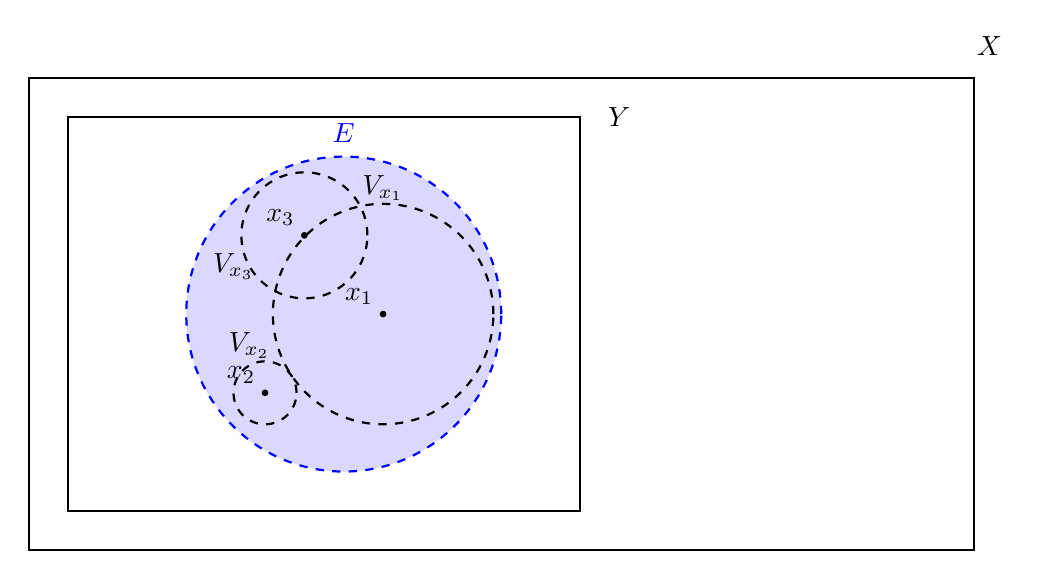
\begin{tikzpicture}
				\draw[color=black, thick] (0,0) rectangle (12,6);
				\draw[color=black, thick] (0.5,0.5) rectangle (7,5.5);
				\draw[black] (7.5,5.5) node {$ Y $};
				\draw (12.2,6.4) node {$ X $};
				\filldraw[color=blue, thick, dashed, fill=blue!15]  (4,3) circle (2cm);
				\draw[blue] (4,5.3) node {$ E $};
				\draw[thick, dashed]  (4.5,3) circle (1.4cm);
				\filldraw (4.5,3) circle (1pt) node[anchor= south east] {${x_1}  $}; 
				\draw (4.5,4.6) node {$V_{x_1} $};
				
				\draw[thick, dashed]  (3,2) circle (.4cm);
				\filldraw (3,2) circle (1pt) node[anchor= south east] {${x_2}  $}; 
				\draw (2.8,2.6) node {$V_{x_2} $};
				\draw[thick, dashed]  (3.5,4) circle (.8cm);
				\filldraw (3.5,4) circle (1pt) node[anchor= south east] {${x_3}  $}; 
				\draw (2.6,3.6) node {$V_{x_3} $};
				
			\end{tikzpicture}
			\caption{We take $ V_x $ to be the neighborhood of $ x $ contained in $ E $. We will always be able to find such a neighborhood because $ E $ is open in $ Y $. In this case, we have shown only three such neighborhoods. The (possibly infinite) union of all such neighborhoods is $ G $, which itself is open.}  
		\end{figure}
	\end{proof}
	\begin{proposition}
		Suppose $ K\subseteq Y\subseteq X $, where $ Y $ and $ X $ are metric spaces. The subset $ K $ is compact in $ X $ \textit{if and only if} $ K $ is compact in $ Y $.  
	\end{proposition}
	\begin{proof}{\color{white}space}
		\begin{enumerate}
			\item[$ (\Longrightarrow) $] Suppose $ K $ is compact in $ X $. Let $ \{V_\alpha\} $ be an arbitrary collection of open sets in $ Y $ which cover $ K $. By Lemma 2.1, there exist sets $ G_\alpha $, open in $ X $, such that $ V_\alpha=Y\cap G_\alpha $ for all $ \alpha $. By the compactness of $ K $, there exists a finite subcover $ \{G_{\alpha_1},\ldots,G_{\alpha_1}\} $. We have $$ K\subseteq\bigcup_{i=1}^n G_{\alpha_i} ,$$ but $ K\subseteq Y $, so $$ K\subseteq\bigcup_{i=1}^n V_{\alpha_i} . $$ This makes $ \{V_{\alpha_1},\ldots,V_{\alpha_1}\} $ a finite subcover, so $ K $ is compact in $ X $. 
			\item[$ (\Longleftarrow) $] Suppose $ K $ is compact in $ Y $. Let $ \{G_\alpha\} $ be an open cover of $ K $ in $ X $. If we let $ V_\alpha=G_\alpha\cap Y $, then $ \{V_\alpha\} $ is an open cover of $ K $ in $ Y $. By the compactness of $ K $ we have a finite subcover $ \{V_{\alpha_1},\ldots,V_{\alpha_n}\} $ in $ Y $. Since $ V_\alpha\subseteq G_\alpha $ for all $ \alpha $, then $ \{G_\alpha\} $ has a finite subcover in $ \{G_{\alpha_1},\ldots,G_{\alpha_n}\} $, so $ K $ is compact in $ X $. 
		\end{enumerate}
		
	\end{proof}
	This result does not seem particularly interesting, but it is novel if you consider open and closed sets. We gave several examples of sets that may be open or closed in some intermediate space, but not a larger space. For instance, $ \Z $ is open in $ \Z $, but it is not open in $ \R $. This result tells us that results like this are not possible with compactness!
	\begin{example}
		Suppose $ E\subseteq \Z $ is compact in $ \Z $. This implies that $ E $ is compact in $ \Q $ and $ \R $. If we had another compact set $ F\subseteq\R $ which is compact in $ \R $, then it is compact in $ \Z $ and $ \Q $ as well. 
	\end{example}
	
	The next two theorems establish that all compact sets are both closed and bounded. This should feel somewhat natural, as compactness can be interpreted as a generalization of closed and bounded sets.
	\begin{theorem}
		Let $ X $ be a metric space, and $ K\subseteq X $ be compact. The set $ K $ is closed. 
	\end{theorem} 
	\begin{proof}
		Let $ K $ be a compact subset of a metric space $ X $. It suffices to show that $ K^c $ is open in $ X $. Suppose $ x\in K^c $, and $ y\in K $. For $ r<\frac{1}{2}d(x,y) $, let $ V_y=N_r(x) $ and $ W_y=N_r(y) $ (Figure 24). For our fixed $ x\in K^c $, we will repeat this process for multiple points in $ K $. By compactness, we know there exists a finite set of $ \{y_1,\ldots,y_n\} $ such that $ \{W_{y_1},\ldots,W_{y_n}\} $ is a finite subcover of $ K $. In constructing this subcover, we also constructed the corresponding sets $ \{V_{y_1},\ldots, V_{y_n}\} $ (Figure 23). If we let $ V=\cap_{i=1}^n V_{y_i} $, then we have $ x\in V\subseteq K^c $, making $ x $ an interior point of $ K^c $. Therefore $ K^c $ is open.
		\begin{figure}[h!]
			\centering
			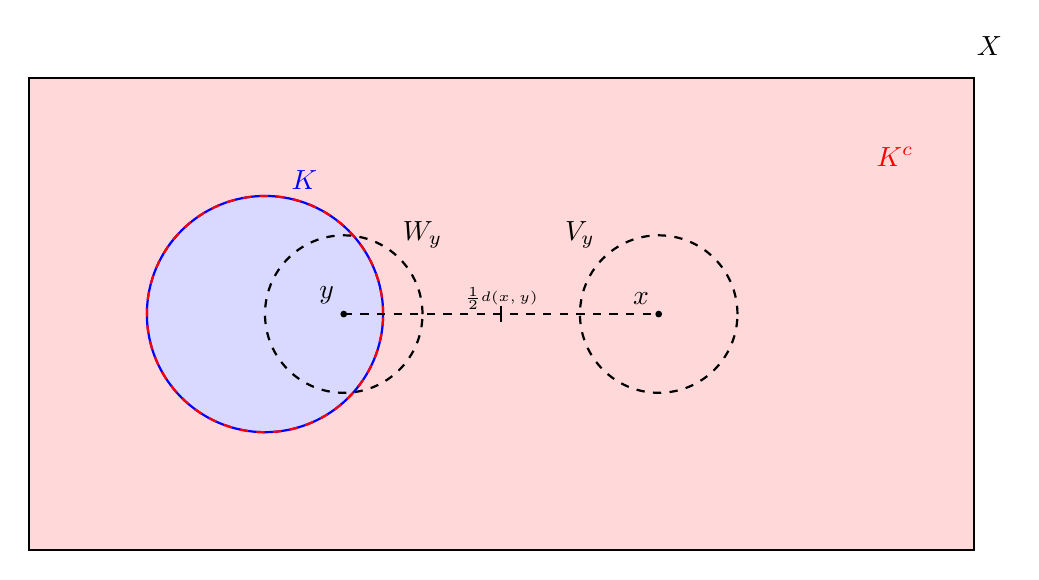
\begin{tikzpicture}
				\filldraw[color=black, thick, fill=red!15] (0,0) rectangle (12,6);
				\filldraw[color=blue, thick, fill=blue!15] (3,3) circle (1.5cm);
				\draw[thick, red, dashed, thick]  (3,3) circle (1.5cm);
				\draw[blue] (3.5,4.7) node {$ K $};
				\draw (12.2,6.4) node {$ X $};
				\draw[red] (11,5) node {$ K^c $};
				\filldraw (4,3) circle (1pt) node[anchor= south east] {$ y $};
				\filldraw (8,3) circle (1pt) node[anchor= south east] {$ x $};
				\draw[thick, dashed] (4,3) circle (1cm);
				\draw[thick, dashed] (8,3) circle (1cm);
				\draw[thick, dashed] (4,3) -- (8,3);
				\draw[thick] (6,3.1)--(6,2.9);  
				\draw[black] (6,3.2) node {\tiny$ \frac{1}{2}d(x,y) $};
				\draw[black] (5,4) node {$ W_{y}$};
				\draw[black] (7,4) node {$ V_{y}$};
			\end{tikzpicture}
			\caption{For some points $ x\in K^c $ and $ y\in K $, we construct neighborhoods $ W_y=N_r(y)$ and $ V_y=N_r(x) $ such that $ r<\frac{1}{2}d(x,y) $. This choice of radius ensures $ V_y\cap W_y=\emptyset $.}  
		\end{figure}
		\begin{figure}[h!]
			\centering
			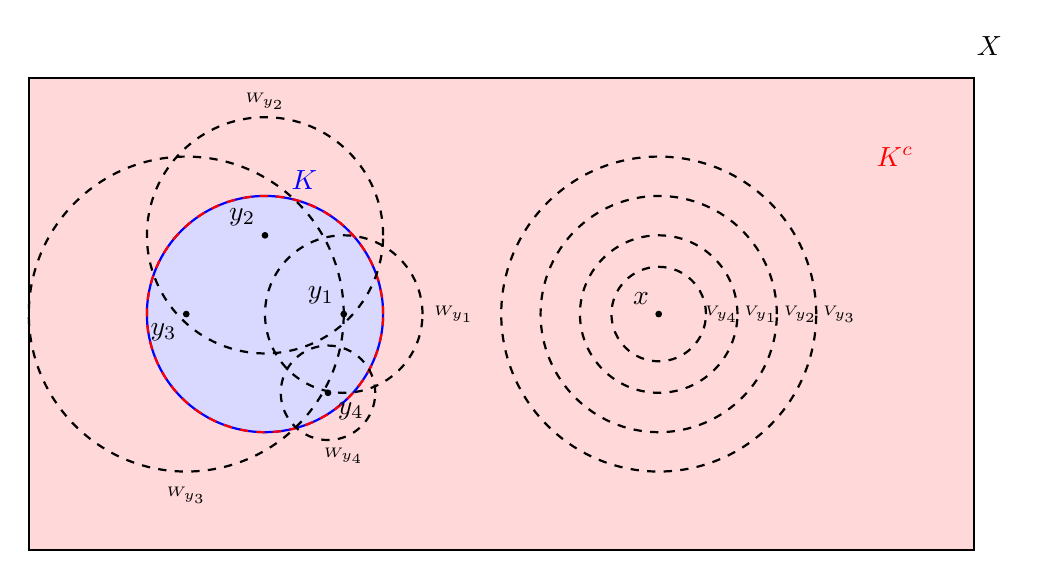
\begin{tikzpicture}
				\filldraw[color=black, thick, fill=red!15] (0,0) rectangle (12,6);
				\filldraw[color=blue, thick, fill=blue!15] (3,3) circle (1.5cm);
				\draw[thick, red, dashed, thick]  (3,3) circle (1.5cm);
				\draw[blue] (3.5,4.7) node {$ K $};
				\draw (12.2,6.4) node {$ X $};
				\draw[red] (11,5) node {$ K^c $};
				\filldraw (4,3) circle (1pt) node[anchor= south east] {$ y_1 $};
				\filldraw (8,3) circle (1pt) node[anchor= south east] {$ x $};
				\draw[thick, dashed] (4,3) circle (1cm);
				\draw[thick, dashed] (8,3) circle (1cm);
				\draw[thick, dashed] (8,3) circle (2cm);
				\draw[thick, dashed] (8,3) circle (0.6cm);
				\draw[thick, dashed] (3.8,2) circle (0.6cm);
				\draw[thick, dashed] (8,3) circle (1.5cm);
				\filldraw (3,4) circle (1pt) node[anchor= south east] {$ y_2 $}; 
				\filldraw (2,3) circle (1pt) node[anchor= north east] {$ y_3 $}; 
				\draw[thick, dashed] (2,3) circle (2cm);
				\draw[thick, dashed] (3,4) circle (1.5cm);
				\filldraw (3.8,2) circle (1pt) node[anchor= north west] {$ y_4 $};
				\draw[black] (8.8,3) node {\tiny$ V_{y_4}$};
				\draw[black] (9.3,3) node {\tiny$ V_{y_1}$};
				\draw[black] (9.8,3) node {\tiny$ V_{y_2}$};
				\draw[black] (10.3,3) node {\tiny$ V_{y_3}$};
				\draw[black] (4,1.2) node {\tiny$ W_{y_4}$};
				\draw[black] (5.4,3) node {\tiny$ W_{y_1}$};
				\draw[black] (3,5.7) node {\tiny$ W_{y_2}$};
				\draw[black] (2,0.7) node {\tiny$ W_{y_3}$};
				
			\end{tikzpicture}
			\caption{For the fixed value $ x\in K^c $, repeat the process illustrated in Figure 21 until we have a finite subcover of $ K $, $ \{W_{y_1},\ldots,W_{y_4}\}.$ If we let $ V $ be the intersection of all $ V_{y_i} $, then $ x\in V\subseteq K^c $, rendering $x $ an interior point of $ K^c $.}  
		\end{figure}
	\end{proof}
	\begin{example}
		The set $ \Q $ in $ \R $ is not closed (Example 2.18), so it is not compact in $ \R $. 
	\end{example}
	
	\begin{theorem}
		Let $ X $ be a metric space, and $ K\subseteq X $ be compact. The set $ K $ is bounded. 
	\end{theorem}
	\begin{proof}
		Let $ x\in K $. The collection of neighborhoods $ \{N_r(x)\} $ for $ r\in\N $ forms an open cover of $ K $. By compactness, this open cover has a finite subcover $ \{N_{r_1}(x),\ldots,N_{r_n}\} $. If we take $ r^*=\max\{r_1,\ldots,r_n\} $, then $ K\subseteq N_{r^*}(x) $, and $ d(x,y)<r^* $ for all $ y\in K $. (Figure 24)
		\begin{figure}[h!]
			\centering
			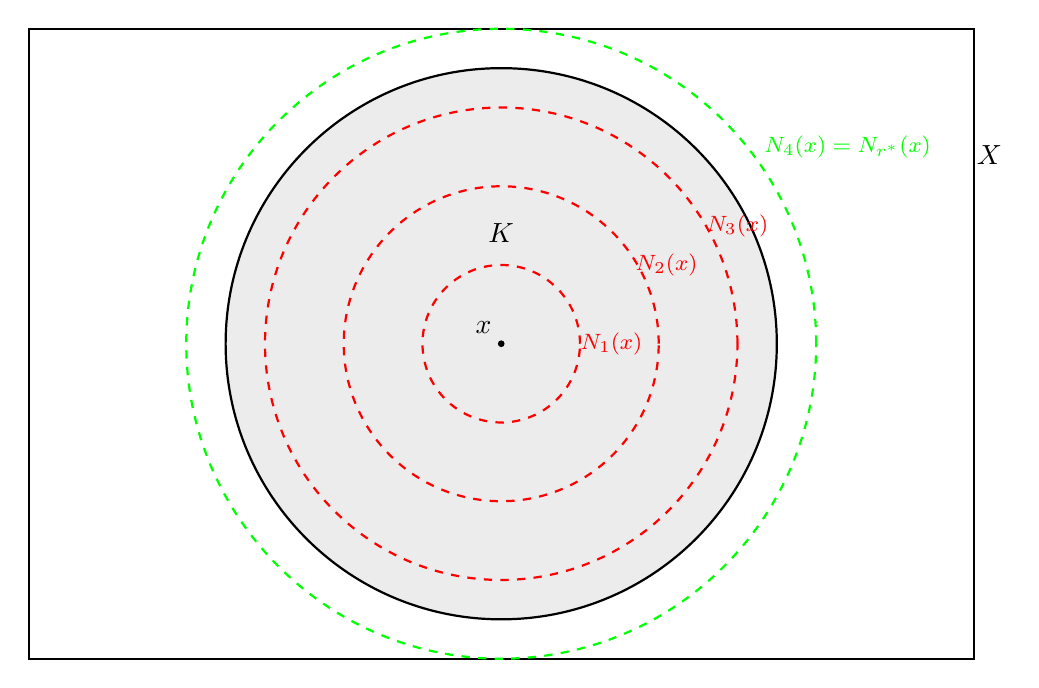
\begin{tikzpicture}
				\draw[color=black, thick] (0,0) rectangle (12,8);
				\filldraw[thick, fill=gray!15] (6,4) circle (3.5cm);
				\draw (12.2,6.4) node {$ X $};
				\draw (6,5.4) node {$ K $};
				\filldraw (6,4) circle (1pt) node[anchor = south east] {$ x $};
				\draw[thick, dashed, red] (6,4) circle (1cm);
				\draw[thick, dashed, red] (6,4) circle (2cm);
				\draw[thick, dashed, red] (6,4) circle (3cm);
				\draw[thick, dashed, green] (6,4) circle (4cm);	
				\draw[red] (7.4,4) node {\footnotesize$ N_{1}(x) $};
				\draw[red] (8.1,5) node {\footnotesize$ N_{2}(x) $};
				\draw[red] (9,5.5) node {\footnotesize$ N_{3}(x) $};
				\draw[green] (10.4,6.5) node {\footnotesize$ N_{4}(x)=N_{r^*}(x) $};
			\end{tikzpicture}
			\caption{We cover the set $ K $ with an infinite open cover comprised of neighborhoods of radii in $ \N $. By compactness there is an open subcover, such as $ \{N_1(x),\ldots,N_4(x)\} $. The set is bounded by the maximum radii $ r^*=4 $ in this finite collection.}  
		\end{figure}
	\end{proof}
	\begin{example}
		The set $ (0,\infty) $ in $ \R $ is not bounded so it is not compact in $ \R $. 
	\end{example}
	\begin{remark}
		While compactness implies closed and bounded, the converse \textit{is not necessarily true}. Soon, we will see that the converse will hold in $ \R^n $, but in general, this is not the case. The next example illustrates this.
	\end{remark}
	\begin{example}
		Let $ X=\{1/n\mid n\in\N\} $ be a metric space equipped with $$ d(x,y)=\begin{cases}
			0\text{ if }x=y\\1\text{ if }x\neq y
		\end{cases}.$$
		The set $ X $ is closed, as it is the whole space. It is also bounded, as $ d(x,y)\le 1 $ for all $ x,y\in X $. Let $ G_n=\{1/n\} $. Each $ G_n $ is open, as $ N_{1/2}(1/n)\subseteq G_n $. This makes $ G_n $ an open cover of $ X $, as $ X\subseteq\bigcup_{n\in \N} G_n=X $. The set $ X $ fails to be compact, because this open cover has no finite subcover. Any finite cover $ \{G_{1},\ldots,G_{N}\} $ would not ``cover''  $ \{1/(N+1),1/(N+2),\ldots\}\subseteq X $.	
	\end{example}
	
	We often restrict our attention to subsets of compact sets, so it would be nice to know if subsets of compact sets are compact. Unfortunately, this is not true in general, but it becomes true if we require the subset satisfy one condition. 
	\begin{proposition}
		Closed subsets of compact sets are compact.
	\end{proposition}
	\begin{proof}
		Suppose $ K $ in $ X $ is compact, and $ F\subseteq K $ is closed in $ X $. Let $ \{V_\alpha\} $ be an arbitrary open cover of $ F $. If we add $ F^c $ to this collection of open sets, we have an open cover $ \Omega=\{V_{\alpha_1},V_{\alpha_2},\ldots,F^c\} $ of $ K $, because $ K=F\cup F^c $. $$ K\subseteq\left(\bigcup_\alpha V_\alpha\right)\cup F^c.$$ The set $ K $ is compact, so there exists a finite open cover of $ \Omega $, $ \Phi=\{V_{\alpha_1},\ldots,V_{\alpha_n}, F^c\} $. We can now remove $ F^c $ from $ \Phi $, resulting in a finite subcover for $ \{V_\alpha\} $. 
	\end{proof}
	\begin{corollary}
		If $ F $ is closed and $ K $ is compact, $ F\cap K $ is compact. 
	\end{corollary}
	An interesting property of compact sets is that if we have a decrease sequence of nested compact intervals, than their intersection is nonempty. This result follows as a corollary of a more general result.
	\begin{proposition}
		If $ \{K_\alpha\} $ is a collection of compact subsets of a metric space $ X $ such that the intersection of every finite subcollection of $ \{K_\alpha\} $ is nonempty, then $ \cap_\alpha K_\alpha\neq\emptyset $. 
	\end{proposition}
	\begin{proof}
		For the sake of contradiction, assume that $ \cap_\alpha K_\alpha=\emptyset $. This means there is some fixed $K_1\in \{K_\alpha\}$ such that no point of $ K_1 $ belongs to every $ K_\alpha $. Let $ G_\alpha= K_\alpha^c $. The collection $ \{G_\alpha\} $ forms an open cover of $ K_1$. Since $ K_1 $ is compact, there exists a finite subcover $ \{G_{\alpha_1},\ldots,G_{\alpha_n}\} $. $$ K\subseteq\bigcup_{i=1}^nG_{\alpha_i}$$ This inclusion, along with the definition of $ G_\alpha $ implies that $ K_1\cap\left(\bigcap_{i=1}^nK_{\alpha_i}\right)=\emptyset $. This contradicts our assumption that every finite subcollection of $ \{K_\alpha\} $ is nonempty. 
	\end{proof}
	\begin{corollary}[Cantor's Intersection Theorem]
		If $ \{K_\alpha\} $ is a sequence of nonempty compact sets such $ K_{n}\supset K_{n+1} $ for $ n\in\N $, then $ \cap_{i=1}^\infty K_n $ is not empty.
	\end{corollary}
	\begin{example}
		Recall that open intervals in $ \R $ are not compact (Example 2.35), and do not satisfy the requirement of Cantor's Intersection Theorem. Let $ G_{n}=(0,1/n) $. We have $ G_{n+1}\subseteq G_{n} $ for all $ n\in\N $, so $ \{G_n\} $ is a decreasing nested sequence of intervals. $$ \cdots\subseteq \left(0,\frac{1}{4}\right)\subseteq\left(0,\frac{1}{3}\right)\subseteq\left(0,\frac{1}{4}\right)\subseteq\left(0,\frac{1}{2}\right)\subseteq(0,1)$$  
		The intersection of these sets is empty.	
	\end{example}
	\begin{proposition}[Bolzano-Weierstrass Property]
		If $ E $ is an infinite subset of a compact set $ K $, then $ E $ has a limit point in $ K $. 
	\end{proposition}
	\begin{proof}
		For the sake of contradiction, assume that no point of $ K $ is a limit point of $ E $. For each $ x\in K $, there exists some $ r $ such that $ V_x=N_r(x)=\{x\}  $ if $ x\in E $, or $ V_x=N_r(x)=\emptyset $ if $ x\notin E $. The collection $ \{V_x\} $ is an open cover of $ E $. The set $ E $ is infinite, so we cannot find a finite subcover for $ \{V_x\} $, as each set is at most a singleton. Because $ E\subseteq K $, the same is true with respect to $ K $, which contradicts the assumption that $ K $ is compact. 
	\end{proof}
	Informally, the Bolzano-Weierstrass Property tells us that we can approximate some point of $ K $ with points in an infinite subset $ E $. Right now, this may not seem significant, but it will become important when we work in $ \R^n $. 
	\begin{remark}
		The Bolzano-Weierstrass Property is often referred to as \textit{\color{red}limit point compactness}. In the context of metric spaces, limit point compactness and compactness are equivalent\footnote{Proving this requires some concepts that are beyond this treatment of metric spaces.}, so in most real analysis texts the prior is never even given a name. As we'll see \textit{much} later on, the two are not equivalent when we explore point-set topology in general (Section 16).   
	\end{remark} 
	\subsection{Compact Sets in $ \R^n $}
	Now we can start working towards sufficient conditions for compactness in $ \R^n $. This will culminate in the famed Heine-Borel Theorem. This theorem establishes sufficient conditions for compactness in $ \R^n $. Specifically, the converses of Theorem 2.3 and Theorem 2.4 will hold in $ \R^n $.  
	
	In order to make the proof of this result a bit more clear, we will show a series of results beforehand which build to the Heine-Borel Theorem.
	\begin{lemma}
		If $ \{I_n\} $ is a sequence of closed intervals in $ \R $, such that $ I_n\supset I_{n+1} $  for $ n\in\N $, then $ \cap_{i=1}^n I_n\neq\emptyset$.
	\end{lemma}  
	\begin{figure}[h]
		\centering
		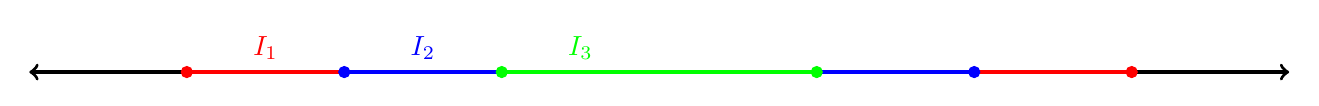
\begin{tikzpicture}
			\draw[very thick, <->] (-8,0) -- (8,0);
			\filldraw[fill=red, color=red] (-6,0)circle (2pt);
			\filldraw[fill=red, color=red] (6,0) circle (2pt);
			\draw[very thick, color = red] (-6,0)--(6,0);
			\draw[red] (-5,.3) node {$ I_1$};
			\filldraw[fill=blue, color=blue] (-4,0)circle (2pt);
			\filldraw[fill=blue, color=blue] (4,0) circle (2pt);
			\draw[very thick, color = blue] (-4,0)--(4,0);
			\draw[blue] (-3,.3) node {$ I_2$};
			\filldraw[fill=green, color=green] (-2,0)circle (2pt);
			\filldraw[fill=green, color=green] (2,0) circle (2pt);
			\draw[very thick, color = green] (-2,0)--(2,0);
			\draw[green] (-1,.3) node {$ I_3$};
		\end{tikzpicture}
		\caption{The first three intervals in the type of sequence $ \{I_n\} $ described in Proposition 2.7.}
	\end{figure}
	\begin{proof}
		Suppose $ I_n=[a_n,b_n] $. Define $ E $ to be the set of all the $ a_n $. The set $ E $ is nonempty and bounded above by $ b_1 $, because $$\cdots a_3\le a_2\le a_1\le b_1\le b_2\le b_3\le \cdots .$$ We have $ E\subseteq \R $ and is bounded, so it has a supremum in $ \R $. Let $ x=\sup E $. For all $ m,n\in\N $, $$a_n\le a_{m+n}\le b_{m+n}\le b_m ,$$ so $ x\le b_m $ for all $ m $. By the definition of $ \sup E $, $ a_m\le x $. If $ x\le b_m $ and $ a_m\le x $, then $ x\in[a_m,b_m]=I_m $ for all $ m\in\N $. Therefore $ x\in\cap_{n\in\N} I_n $.
	\end{proof}
	\begin{example}
		If we modify Example 2.42 so the open intervals are closed, then we have a sequence $ \{I_n\} $ where $ I_n=[0,1/n] $. This gives $ \cap_{n\in\N} I_n=\{0\}\neq\emptyset $. If we worked through the proof of Lemma 2.2 with this particular example, we would find that $ 0 $ is the supremum of the set of lower bounds of $ I_n $. 
	\end{example}
	This result should look familiar. Cantor's Intersection Theorem states a similar result for compact sets. This in and of itself does not show that closed intervals are compact, but it should catch our attention, as closed intervals and compact sets share a noteworthy property. It should also be noted that this property of closed intervals follows from the least-upper-bound property of $ \R $. This is one of the magical results we get because $ \R $ is complete.  We can generalize Proposition 2.7 to \textit{\color{red}$ k $-cells} in $ \R^k $. An  $ k $-cell is the set of all points $ \x=(x_1,\ldots,x_k)\in\R^k $ which satisfy $ a_i\le x_i\le b_i $ for $ i=1,\ldots,k $, where $ a_i,b_i\in\R $, and $ a_i\le b_i $. 
	\begin{lemma}
		Let $ k\in\N $. If $ \{I_n\} $ is a sequence of $ k- $cells such that $ I_n\supset I_{n+1} $ for all $ n\in\N $, then $ \cap_{n\in\N} I_n\neq\emptyset $. 
	\end{lemma}
	\begin{figure}[h]
		\centering
		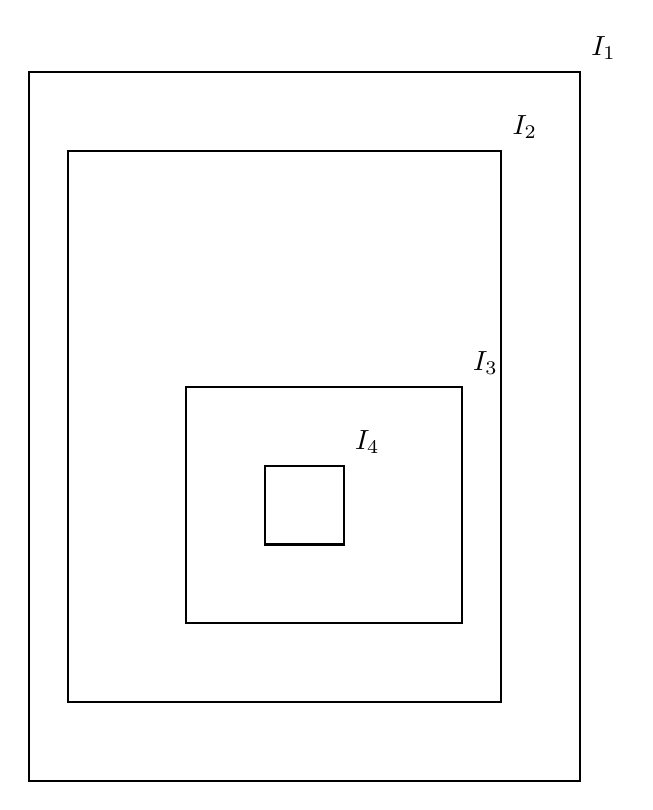
\begin{tikzpicture}
			\draw[thick] (0,0) rectangle (7,9);
			\draw (7.3,9.3) node {$ I_1$};
			\draw[thick] (0.5,1) rectangle (6,8);
			\draw (6.3,8.3) node {$ I_2$};
			\draw[thick] (2,2) rectangle (5.5,5);
			\draw (5.8,5.3) node {$ I_3$};
			\draw[thick] (3,3) rectangle (4,4);
			\draw (4.3,4.3) node {$ I_4$};
		\end{tikzpicture}
		\caption{The first four $ 2- $cells in the type of sequence $ \{I_n\} $ described in Proposition 2.8.}
	\end{figure}
	\begin{proof}
		Let $ I_n $ be the set of points $ \x=(x_1,\ldots,x_k) $ such that $ a_{n,j}\le x_j\le b_{n,j} $ for $ j=1,\ldots, k $ and $ n\in\N $, and write $ I_{n,j}=[a_{n,j},a_{b,j}] $. By Lemma 2.2, for each $ I_{n,j} $, $ \cap_{n\in\N}I_{n,j}\neq\emptyset $, so there is some $ x_j^*\in\cap_{n\in\N} I_{n,j} $ which satisfies $$ a_{n,j}\le x_j^*\le b_{n,j}$$ for $j=1,\ldots, k $ and $ n\in\N $. If we set $ \x^*=(x_1^*,\ldots,x_k^*) $, then $ \x^*\in I_n $ for all $ n\in\N $. Therefore  $ \cap_{n\in\N} I_n\neq\emptyset $. 
	\end{proof}
	We will now prove that each $ k -$cell is compact. The definition of a $ k -$cell is equivalent to a closed and bounded set in $ \R $, so this result will give us our sufficient conditions for compactness in $ \R^n $. This result will give rise to the Heine-Borel Theorem which is an equivalence result, which will follow immediately from the compactness of $ k $-cells, Theorem 2.3, and Theorem 2.4. That being said, the proof that each $ k -$cell is compact is not immediate, and is on the more difficult side for a proof in an introductory analysis course.    
	\begin{lemma}
		Every $ k -$cell is compact. 
	\end{lemma}
	\begin{proof}
		Let $ I=\{\x\in\R^k\mid a_j\le x_j\le b_j\ j=1,\ldots,k\} $ be a $ k- $cell. Let $ \delta $ be the maximum distance between any two points in $ I $.
		$$ \max\limits_{\x,\y\in I}d(\x,\y)=\delta=\left(\sum_{j=1}^k(b_j-a_j)^2\right)^{1/2}$$
		For all $ \x,\y\in I $, $ |\x-\y|\le\delta $ (Figure 27 shows this for $ k=2 $). 
		\begin{figure}[h!]
			\centering
			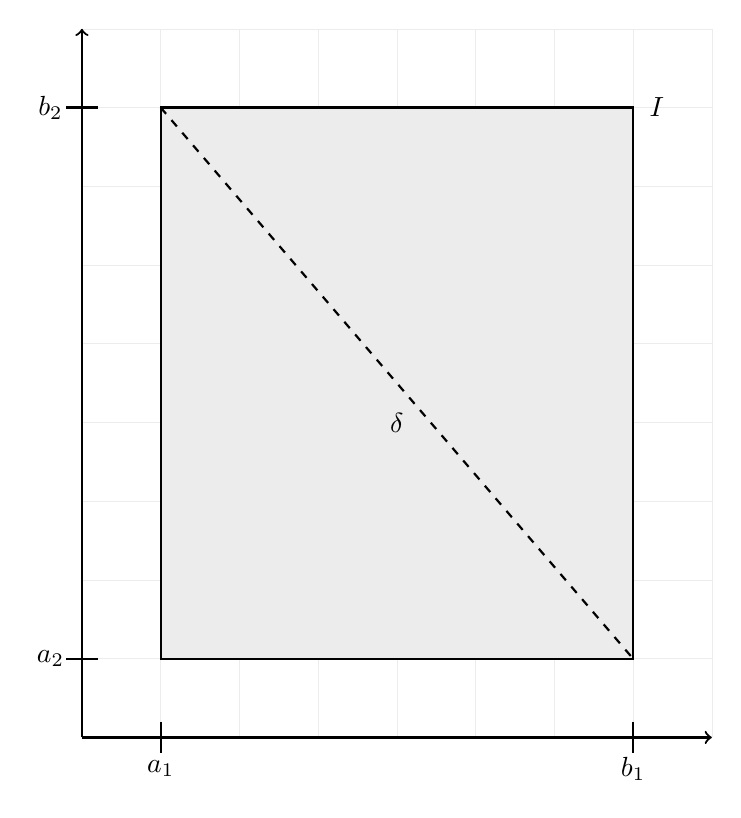
\begin{tikzpicture}
				
				\draw[step=1cm,gray!15,very thin] (0,0) grid (8,9);
				\filldraw[thick, fill = gray!15] (1,1) rectangle (7,8);
				\draw (7.3,8) node {$ I$};	
				\draw[thick,->] (0,0) -- (0,9);
				\draw[thick,->] (0,0) -- (8,0);
				\draw[thick] (1,0.2) -- (1,-0.2);
				\draw[thick] (7,0.2) -- (7,-0.2);
				\draw[thick] (-0.2,1) -- (0.2,1);
				\draw[thick] (-0.2,8) -- (0.2,8);
				\draw (1,-0.4) node {$ a_1$};	
				\draw (7,-0.4) node {$ b_1$};
				\draw (-0.4,1) node {$ a_2$};
				\draw (-0.4,8) node {$ b_2$};
				\draw[thick, dashed] (1,8) -- (7,1) ;
				\draw (4,4) node {$ \delta $};
			\end{tikzpicture}
			\caption{If $ I $ is a 2-cell.}
		\end{figure}
		
		For the sake of contradiction, assume that there exists some arbitrary open cover $ \{G_\alpha\} $ of $ I $ which contains no finite subcover of $ I $. Let $ c_j=(a_j+b_j)/2 $. The intervals $ [a_j,c_j] $ and $ [c_j,b_j] $ give rise to $ 2^k $ $ k $-cells $ Q_i $ whose union is $ I $. If each of these cells $ Q_i $ could be covered by a finite subcollection of $ \{G_\alpha\} $, then $ I $ could be covered by the union of all these finite subcollections, which is finite. Since we've assumed $ K $ is not compact, then it must be that there exists at least one $ Q_i $, call it $ I_1 $, that cannot be covered by any finite subcollection of $ \{G_\alpha\} $.  
		\begin{figure}[h!]
			\centering
			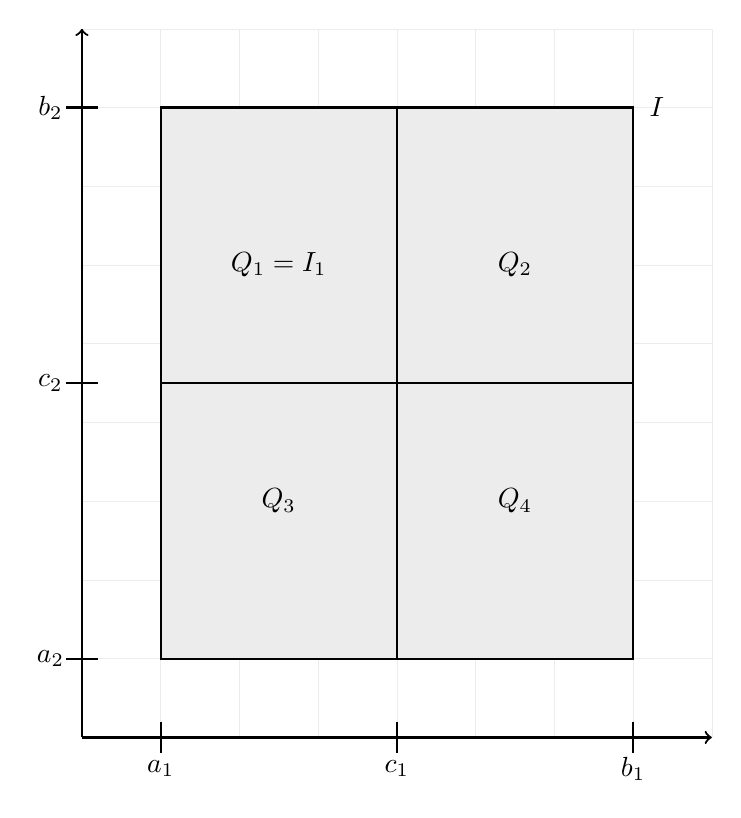
\begin{tikzpicture}
				
				\draw[step=1cm,gray!15,very thin] (0,0) grid (8,9);
				\filldraw[thick, fill = gray!15] (1,1) rectangle (7,8);
				\draw (7.3,8) node {$ I$};	
				\draw[thick,->] (0,0) -- (0,9);
				\draw[thick,->] (0,0) -- (8,0);
				\draw[thick] (1,0.2) -- (1,-0.2);
				\draw[thick] (7,0.2) -- (7,-0.2);
				\draw[thick] (-0.2,1) -- (0.2,1);
				\draw[thick] (-0.2,8) -- (0.2,8);
				\draw (1,-0.4) node {$ a_1$};
				\draw (4,-0.4) node {$ c_1$};	
				\draw (7,-0.4) node {$ b_1$};
				\draw (-0.4,1) node {$ a_2$};
				\draw (-0.4,8) node {$ b_2$};
				\draw (-0.4,4.5) node {$ c_2$};
				\draw[thick] (-0.2,4.5) -- (0.2,4.5);
				\draw[thick] (4,0.2) -- (4,-0.2);
				\draw[thick] (1,4.5)-- (7,4.5);
				\draw[thick] (4,1)-- (4,8);
				\draw (2.5,3) node {$ Q_3$};
				\draw (5.5,3) node {$ Q_4$};
				\draw (2.5,6) node {$ Q_1=I_1$};
				\draw (5.5,6) node {$ Q_2$};
			\end{tikzpicture}
			\caption{We partition $ I $ into $ 2^k $ cells $ Q_i $. If $ I $ is not compact, then there is some $ Q_i $ which is not compact. Suppose in this case $ Q_1 $ is not compact, and call it $ I_1 $. }
		\end{figure}
		Now we divide $ I_1 $ into $ 2^k $ $ k -$cells and repeat this process indefinitely, giving us a sequence $ \{I_n\} $ (Figure 29). 
		\begin{figure}[h!]
			\centering
			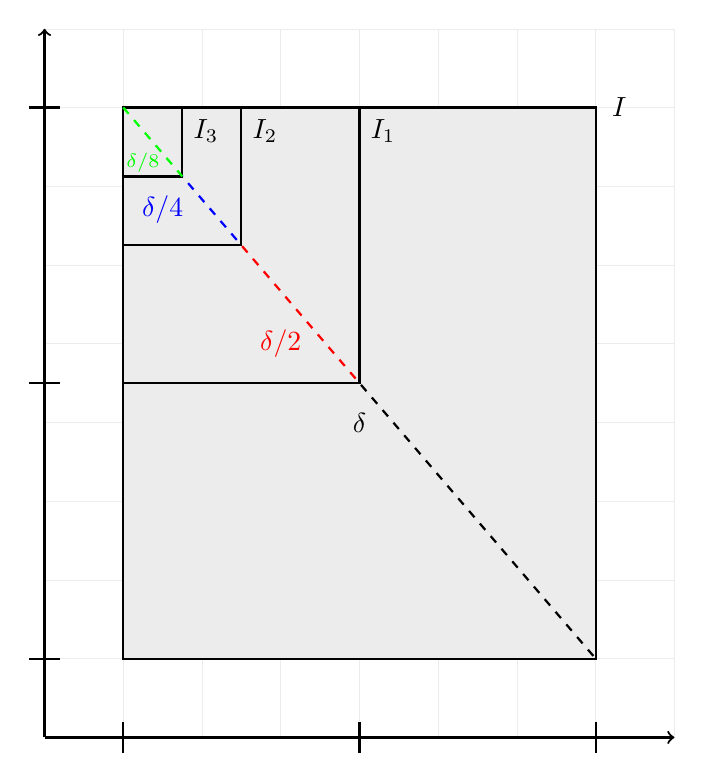
\begin{tikzpicture}
				
				\draw[step=1cm,gray!15,very thin] (0,0) grid (8,9);
				\filldraw[thick, fill = gray!15] (1,1) rectangle (7,8);
				\draw (7.3,8) node {$ I$};	
				\draw[thick,->] (0,0) -- (0,9);
				\draw[thick,->] (0,0) -- (8,0);
				\draw[thick] (1,0.2) -- (1,-0.2);
				\draw[thick] (7,0.2) -- (7,-0.2);
				\draw[thick] (-0.2,1) -- (0.2,1);
				\draw[thick] (-0.2,8) -- (0.2,8);
				
				\draw[thick, dashed] (1,8) -- (7,1) ;
				
				\draw (4,4) node {$ \delta $};
				\draw[thick] (-0.2,4.5) -- (0.2,4.5);
				\draw[thick] (4,0.2) -- (4,-0.2);
				\filldraw[thick, fill = gray!15] (1,4.5) rectangle (4,8);	
				\draw[thick, dashed, red] (1,8) -- (4,4.5) ;
				\filldraw[thick, fill = gray!15] (1,6.25) rectangle (2.5,8);
				\draw[thick, dashed, blue] (1,8) -- (2.5,6.25) ;
				\filldraw[thick, fill = gray!15](1,7.125) rectangle (1.75,8);
				\draw[thick, dashed, green] (1,8) -- (1.75,7.125) ;
				\draw (4.3,7.7) node {$ I_1$};
				\draw (2.8,7.7) node {$ I_2$};
				\draw (2.05,7.7) node {$ I_3$};
				\draw[red] (3,5) node {$ \delta/2 $};
				\draw[blue] (1.5,6.7) node {$ \delta/4 $};
				\draw[green] (1.25,7.3) node {\scriptsize$ \delta/8 $};
			\end{tikzpicture}
			\caption{The first three $ 2 $-cells in the sequence $ \{I_n\} $.}
		\end{figure}
		This sequence of $ k $-cells was constructed to have three properties:
		\begin{enumerate}
			\item $ I\supset I_1\supset I_2\supset I_3\supset\cdots $
			\item $ I_n $ cannot be covered by any finite subcollection of $ \{G_\alpha\} $, otherwise $ K $ would not be compact.\footnote{This follows from the same reasoning applied to the $ 2^k $ $ k $-cells $ Q_i $ we initially chose $ I_1 $ from.}
			\item If $ \x,\y\in I_n $, then $ |\x-\y|\le \delta/2^n $.\footnote{When we divided $ I $, the length of the diagonal for $ I_1 $ became half of $ \delta $. When we divide $ I_1 $, the length of the diagonal of $ I_2 $ became half of that of $ I_1 $. This means we can always write the diagonal of $ I_n $ in terms of powers of $ 1/2 $ and $ \delta $.  }
		\end{enumerate}
		By the first property of this sequence, we can invoke Lemma 2.3 to determine $ \cap_{n\in\N} I_n\neq\emptyset $. This means there exists some $ \x^*\in\R^k $ such that $ \x^*\in I_n $ \textit{for all} $ n\in\N $. There must be some $ \alpha $ such that $ \x^*\in G_\alpha $, otherwise $ \{G_\alpha\} $ would not be an open cover of $ I $. Since $ G_\alpha $ is open, there exists some $ r>0 $ such that $ N_r(x)\subseteq G_\alpha $. Alternatively, we could say that $ |\y-\x^*|<r $ implies $ y\in G_\alpha $ by the definition of $ N_r(x) $. If we take $ n $ to be so large that $ \delta/2^n<r $,\footnote{We can always find such an $ n $. If not, $ 2^n\le\delta /r $ for all $ n \in\N$. This can't be though because $ \R $ has the Archimedean property (Theorem 1.3).} then $ I_n\subseteq G_\alpha $, but this would mean $ I_n $ has a finite subcover. This contradicts property $ 2 $ of our sequence $ \{I_n\} $, thereby contradicting the assumption that $ K $ is not compact. 
	\end{proof}
	\begin{example}
		In order to make this proof a bit more concrete we'll walk through it with the $ 2 $-cell define by $ I=[0,1]\times[0,1] $, and a specific open cover.\footnote{In order to give such an example, we need to specify an open cover to work with. In doing so, we're sort of shooting ourselves in the foot. The whole point of compactness is that \textit{every} open cover has a finite subcover. What we're really proving in this example, is this specific open cover has no finite subcover.} Let our open cover $ G_\alpha=N_{0.01}(\alpha)  $ for $ \alpha\in I $. $$ I\subseteq \bigcup_{\alpha\in I} G_\alpha=\bigcup_{\alpha\in I}N_{0.01}(\alpha)$$  Assume that this open cover has no finite subcover. We have $$ \delta=((1-0)^2+(1-0)^2)^{1/2}=\sqrt{2} .$$ We divide $ I $ into four $ 2 $-cells: $ Q_1=[0,1/2]\times[0,1/2] $, $Q_2=[0,1/2]\times[1/2,1]$, $ Q_3=[0.5,1]\times[0,1/2] $, and $ Q_4=[1/2,1]\times[1/2,1] $. If $ \{G_\alpha\} $ has no finite subcover for $ I $, then the same can be said for one of these $ Q_i $. Suppose this is the case for $ Q_1 $, and let $ I_1=Q_1=[0,1/2]\times[0,1/2] $. Repeat this process seven times until we arrive at $ I_7=[0,1/256]\times[0,1/256] $. The maximum distance between any two points in $ I_7 $ is $$ \left((1/256-0)^2+(1/256-0)^2\right)^{1/2}\approx0.0055<0.01.$$ Therefore, we can cover $ I_7 $ with a single $ N_{0.01}(\alpha) \in\{G_\alpha\}$ for any $ \alpha\in I_7 $. But this means we can cover $ I_6 $ with four elements in $ \{G_\alpha\} $,\footnote{I'm playing a little fast and loose here with which exact elements, because I'm not specifying where the neighborhoods are centered.}  and cover $ I_5 $ with $ 4^2 $ elements in $ \{G_\alpha\}  $, etc. We can cover $ I $ with $ 4^7 $ elements in $ \{G_\alpha\} $. This contradicts the assumption that $ \{G_\alpha\} $ has no finite subcover. 
		
		One of the subtler, but nevertheless important, parts of this process is that we could repeatedly divide the cells until we found a cell that fit in a neighborhood of radius $ 0.01 $. We will always be able to do this because of the Archimedean property as discussed in Footnote 22. It is important, that you do not associate this particular ``trick'' with the fact that $ I $ is a subset of $ \R^2 $. We are discussing the Archimedean property in the context of distances and radii, so we're actually using the fact that $ \R^2  $ is equipped with a distance function $ d:\R^2\times\R^2\to[0,\infty] $. We're using the fact that the codomain of $ d $ has the Archimedean property!  
	\end{example}
	We have now shown that every $ k $-cell is compact. The proof is made more manageable with illustrations, but is still rather technical. Our contradiction came from the fact that as $ n $ becomes large, $ I_n $ becomes small. Eventually $ I_n $ will be so small, that it must have a finite open subcover. This contradicts the assumption that $ I $ is not compact. 
	\begin{theorem}[Heine-Borel Theorem]
		A set $ E $ in $ \R^n $ is compact \textit{if and only if} it is closed and bounded.
	\end{theorem} 
	\begin{proof}{\color{white}space}
		\begin{enumerate}
			\item [$ (\Longrightarrow) $] All compact sets are closed and bounded by Theorems 2.3 and 2.4. 
			\item [$ (\Longleftarrow) $] If $ E $ is closed and bounded then $ E\subseteq I $ for some $ n -$cell. Any closed subset of a compact set is compact by Proposition 2.4, so $ E $ is compact.
		\end{enumerate}
	\end{proof}
	\begin{example}
		Any closed interval $ [a,b]\subseteq \R$ is compact. 
	\end{example}
	\begin{theorem}[Bolzano–Weierstrass Theorem]
		Every bounded infinite subset of $ \R^n $ has a limit point in $ \R^n $. 
	\end{theorem}
	\begin{proof}
		Let $ E\subseteq\R^n $ be bounded and infinite. There is some $ n $-cell $ I\subseteq\R^k $, such that $ E\subseteq I $. By Lemma 2.4 $ I $ is compact. We know apply Proposition 2.6 to conclude that $ E $ has a limit point in $ I $, which is also in $ \R^k $.
	\end{proof}
	\begin{example}
		The set $ (a,b)\subseteq\R $ is infinite and bounded. It has an infinite number of limit points in $ \R^n $,\footnote{In fact, the set of limit points is $ [a,b]\subseteq\R $} including $ a $ and $ b $.
	\end{example}
	\subsection{Exercises}
	\begin{ex}
		Show that the set of all algebraic numbers is countably infinite.
	\end{ex}
	\begin{ex}
		Show that the set of all binary numbers with infinite digits is uncountably infinite.
	\end{ex}
	\begin{ex}
		Verify that the taxi-cab metric on $ \R^n $ is a valid metric space.
	\end{ex}
	\begin{ex}
		Let $ X $ be an infinite set with the metric, $$d(x,y)=\begin{cases}
			1\text{ if }x\neq y\\
			0\text{ if }x=y
		\end{cases} .$$ Prove that $ (X,d) $ is a metric space. Which subsets of $ X $ are open? Which are closed? 
	\end{ex}
	\begin{ex}
		Prove that $ E^\circ $ is open.
	\end{ex}
	\begin{ex}
		Prove that $ E $ is open \textit{if and only if} $ E=E^\circ $.
	\end{ex}
	\begin{ex}
		If $ G\subseteq E $ and $ G $ is open, prove that $ G\subseteq E^\circ $
	\end{ex}
	\begin{ex}
		Prove that $ (E^\circ)^c=\overline{E^c} $.
	\end{ex}
	\begin{ex}
		Find an example of a set $ E  $ in a metric space such that $ E^\circ\neq(\bar{E} )^\circ$.
	\end{ex}
	\begin{ex}
		Find an example of a set $ E  $ in a metric space such that $ \bar{E}\neq\overline{E^\circ}$.
	\end{ex}
	\begin{ex}
		Prove that $ \partial E $ is closed.
	\end{ex}
	\begin{ex}
		Prove that $ \partial(E^\circ)\subseteq \partial E  $, and $ \partial(\bar{E})\subseteq \partial E  $
	\end{ex}
	\begin{ex}
		Prove that $ \partial E=\partial (E^c)  $.
	\end{ex}
	\begin{ex}
		Suppose $ E $ is closed. Show that $ (\partial E)^\circ=\emptyset $. 
	\end{ex}
	\begin{ex}
		Prove that $ \partial (\partial E)\subseteq \partial E $. When will the sets be equal? 
	\end{ex}
	\begin{ex}
		Prove that $ E $ is closed \textit{if and only if} $ E\cap \partial E=\emptyset $.
	\end{ex}
	\begin{ex}
		Prove that $ \partial E=\emptyset$ \textit{if and only if} $ E $ is closed and open.  
	\end{ex}
	\begin{ex}
		Prove that $ \bar{E}=E\cup\partial E $.
	\end{ex}
	\begin{ex}
		Prove that $ (\partial \bar{E})^\circ=\emptyset $. 
	\end{ex}
	\newpage
	\section{Sequences and Series}
	Now that we are intimately familiar with the behavior of metric spaces, we can discuss a topic that may be familiar from calculus -- sequences and series. Metric spaces will allow us to rigorously define convergence, and the properties related to the convergence os sequences and series. While we will derive some results and examples in general metric spaces, we will also start introducing results specific to $ \R $.       
	\subsection{Convergence}
	\begin{definition}\label{def}
		Let $ X $ be a metric space. A \textit{\color{red}sequence $ \{x_n\} $} is an function from $ f:\N\to X $. We will sometimes refer to an entire sequence as $  x_n=f(n)$. 
	\end{definition}
	Using an arbitrary metric space $ X $ in this definition means that we, once again, always need to pay attention to what metric space we are in. We saw this with open sets, closed sets, and compact sets, and we will see it again. It will become especially relevant when determining if sequences converge. 
	\begin{example}
		Let $ x_n=1/n$ be a sequence in $ \R $. The first several terms in this sequence are $$ 1,\frac{1}{2},\frac{1}{3},\frac{1}{4},\ldots.$$
		This set is also a sequence in $ \Q $. This sequence is not defined in $ \Z $ or $ \N $, as neither of these sets has fractions.  
	\end{example}
	\begin{example}
		Let $ x_n=2 $ be a sequence in $ \R $. This constant sequence always takes on the value $ 2$. This sequence is also a sequence in $ \N,\Z $, and $ \Q $.
	\end{example}
	\begin{example}
		Let $ x_n=(-1)^n $ be a sequence in $ \R $. This sequence alternates between $ -1 $ and $ 1 $ for all values in $ \N $.  
	\end{example}
	
	Now we are ready to formalize what it means for a sequence to converge. When the idea of convergence is first introduced, you often hear phrases like ``arbitrarily close''. If a sequence converges to some point $ x\in X $, we can \textit{always} get closer to $ x $. For any value in $ \{x_n\}$, we can find other points ``later'' in the sequence $ \{x_n\} $ that is even closer. If convergence is a recipe, then these are the ingredients:  
	\begin{enumerate}
		\item No matter how ``close'' we get, we can always get closer with another point in $ \{x_n\} $. Fortunately, we're in a metric space $ (X,d) $, so we can use $ d $ to determine how close we are.
		\item Well actually, it cannot be \textit{any} other points ``later'' in $ \{x_n\} $. For instance, suppose we have the following sequence: $$ 1, \frac{1}{2}, 2, \frac{1}{3}, 3, \frac{1}{4}, 4,\ldots . $$ The even terms of this series are getting closer to $ 0 $, while the odd terms are growing. The latter fact means this sequence doesn't converge. This happens because not \textit{all} the points ``later'' in $ \{x_n\} $ are closer.  
	\end{enumerate} 
	These two ingredients will correspond to the $ \varepsilon $ and $ N $ in our definition.
	\begin{definition}\label{def}
		A sequence $ \{x_n\} $ in a metric space $ X $ \textit{\color{red}converges (in $ X $)} if there exists an $ x\in X $ such that \textit{for all }$ \varepsilon>0 $, there is an $ N\in\N $ such that $ d(x_n,x)<\varepsilon $ \textit{for all} $ n\ge N $. We will call $ x $ the \textit{\color{red}limit} of $ \{x_n\} $, and write either $ x_n\to x $, or $$\lim\limits_{n\to\infty} x_n=x. $$
	\end{definition}
	\begin{figure}[h!]
		\centering
		\begin{tikzpicture}
			\draw (-.3,9) node {$ \R$};
			\draw (16,-0.3) node {$ \N$};		
			\draw[thick,->] (0,0) -- (0,9);
			\draw[thick,->] (0,0) -- (16,0);
			\draw[thick,dashed] (0,4.5) -- (16,4.5);
			\draw (-.3,4.5) node {$ x$};
			\draw[red] (5,1) node {$ n<N$};
			\draw[green] (12,1) node {$ n\ge N$};
			\draw[thick,dashed] (0,5) -- (16,5);
			\draw[thick,dashed] (0,4) -- (16,4);
			\draw (-.5,4) node {$ x-\varepsilon$};
			\draw (-.5,5) node {$ x+\varepsilon$};
			\filldraw[red] (0.4,1) circle (2pt);
			\filldraw[red] (0.8,8) circle (2pt);
			\filldraw[red] (1.2,1.5) circle (2pt);
			\filldraw[red] (1.6,7.5) circle (2pt);
			\filldraw[red] (2.0,2) circle (2pt);
			\filldraw[red] (2.4,7) circle (2pt);
			\filldraw[red] (2.8,2.2) circle (2pt);
			\filldraw[red] (3.2,6.8) circle (2pt);
			\filldraw[red] (3.6,2.4) circle (2pt);
			
			\filldraw[red] (4,6.6) circle (2pt);
			\filldraw[red] (4.4,2.6) circle (2pt);
			\filldraw[red] (4.8,6.4) circle (2pt);
			\filldraw[red] (5.2,2.8) circle (2pt);
			\filldraw[red] (5.6,6.2) circle (2pt);
			
			\filldraw[red] (6,3.0) circle (2pt);
			\filldraw[red] (6.4,6) circle (2pt);
			\filldraw[red] (6.8,3.2) circle (2pt);
			\filldraw[red] (7.2,5.8) circle (2pt);
			\filldraw[red] (7.6,3.4) circle (2pt);
			\filldraw[red] (8,5.6) circle (2pt);
			
			\filldraw[red] (8.4,3.6) circle (2pt);
			\filldraw[red] (8.8,5.4) circle (2pt);
			\filldraw[red] (9.2,3.8) circle (2pt);
			\filldraw[red] (9.6,5.2) circle (2pt);
			\filldraw[red] (10,4) circle (2pt);
			\filldraw[red] (10.4,5) circle (2pt);				
			\draw[thick,dashed] (10.8,0) -- (10.8,9);
			\draw (10.8,-0.3) node {$ N$};			
			\filldraw[green] (10.8,4.2) circle (2pt);
			\filldraw[green] (11.2,4.8) circle (2pt);
			\filldraw[green] (11.6,4.4) circle (2pt);
			\filldraw[green] (12,4.6) circle (2pt);
			\filldraw[green] (12.4,4.6) circle (2pt);
			\filldraw[green] (12.8,4.4) circle (2pt);
			\filldraw[green] (13.2,4.4) circle (2pt);
			\filldraw[green] (13.6,4.6) circle (2pt);
			\filldraw[green] (14,4.6) circle (2pt);
			\filldraw[green] (14.4,4.4) circle (2pt);	
			\filldraw[green] (14.8,4.45) circle (2pt);
			\filldraw[green] (15.2,4.55) circle (2pt);
			\filldraw[green] (15.6,4.475) circle (2pt);
			\filldraw[green] (16,4.525) circle (2pt);
			
			
		\end{tikzpicture}
		\caption{A convergent sequence $ \{x_n\} $ in $ \R $. No matter how small we take $ \varepsilon $ to be, we can always find some $ N $ such that all $ d(x_n,x)=|x_n-x|<\varepsilon $ for all $ n\ge N $. We could also write $ x_n\in N_\varepsilon(x)=(x-\varepsilon,x+\varepsilon) $. }
	\end{figure}
	We can think of the convergence of a sequence in the context of a hypothetical game. Suppose you and a friend have some convergent sequence $ \{x_n\} $ in $ X $. Your friend says some small number $ \varepsilon $, and challenges you to find an $ N $ such that $ d(x_n,x)<\varepsilon $ for all $ n\ge N $. By the definition of convergence, you can do this. This frustrates your friend, so he demands you do it for an even smaller value of $ \varepsilon $. Unfortunately for him, you will always be able to find such an $ N $. No matter how small $ \varepsilon $ is, you will be able to do this. 
	\begin{remark}
		We can formulate an equivalent definition of convergence using neighborhoods. If for all  $ \varepsilon>0 $, $ d(x_n,x)<\varepsilon $ whenever $ n\ge N $, then we could also say $ x_n\in N_\varepsilon(x) $ for all $ n\ge N $. 
	\end{remark}
	
	\begin{example}
		The sequence $ x_n=1/n $ converges to $ 0 $ in $ \R $. Suppose your friend lets $ \varepsilon=0.01 $, and asks you to find an $ N\in\N $ such that $$ d(1/n,0)=|1/n-0|=1/n<\varepsilon=0.01 $$ for all $ n\ge N $. If you let $ N=101 $, then you have done this. \begin{align*}
			1/101&<0.01\\1/102&<0.01\\1/103&<0.01\\&\vdots
		\end{align*} 
		Your friend then gives you $ \varepsilon=0.001 $. In this case, let $ N=1001 $.
		\begin{align*}
			1/1001&<0.01\\1/1002&<0.01\\1/1003&<0.01\\&\vdots
		\end{align*} 
		You're already bored of this game, so you get an idea. Maybe you can find some function of $ \varepsilon $ that will give you your value of $ N $. In order to do this, you just manipulate the inequality you must satisfy.
		\begin{align*}
			d(1/n,0)&<\varepsilon\\|1/n-0|&<\varepsilon\\1/n&<\varepsilon\\n&>\varepsilon^{-1}		
		\end{align*}
		We just let $ N=\varepsilon^{-1}+1 $. This way, for all $ n\ge N $, we have $ n>\varepsilon^{-1} $, which implies $ d(1/n,0)<\varepsilon $. 
	\end{example}
	\begin{remark}
		The definition of convergence has two inequalities. The inequality $ d(x_n,x)<\varepsilon $ is strict, while $ n\ge N $ is not. In the grand scheme of things, it doesn't matter if these are strict or not. If we instead had $ d(x_n,x)\le\varepsilon $, then we could just have taken $ N=\varepsilon^{-1} $ in the previous example. Alternatively, if we had $ d(x_n,x)<\varepsilon $ and $ n>N $, then $ N=\varepsilon^{-1} $ would work as well. I'm going to try very hard to stick with the inequalities in the definition, but I may make a mistake. Just know that it doesn't change the results of proofs at all. It does mean we need to be a little careful when using neighborhoods though, because they are open set.   
	\end{remark}
	\begin{example}
		We can verify that the sequence $ x_n=(n+1)/(n-1) $ converges to $ 1 $ in $ \R $. Let $ \varepsilon>0 $. We want to find the value of $ N $ in terms of $ \varepsilon $ that satisfies $ d(x_n,x)<\varepsilon $ for all $ n\ge N $. First notice that $$d(x_n,x)=\left\lvert\frac{n-1}{n+1}-1\right\rvert=\left\lvert\frac{-2}{n+1}\right\rvert=\frac{2}{n+1} .$$
		We can satisfy $ \frac{2}{n+1}<\varepsilon $ with $ N=2/\varepsilon-1 $.\footnote{You may be thinking that it isn't always true that this $ N $ will be in $ \N $. That's fine. We could just round the answer to get a whole number that satisfies the inequality. Generally, we're not too worried about this.} We have that $ d(x_n,x)<\varepsilon $ for all $ n\ge 2/\varepsilon-1 $. 
	\end{example}
	\begin{example}
		Let $ \Z $ be a metric space equipped with the $ p $-adic metric (see Example 2.4). The sequence $ x_n=p^n $ converges to $ 0 $ for any prime $ p $. We have $$d(x_n,0)=p^{-\max\{ m\in\N\ |\ p^m\mid (p^n-0) \}}=p^{-n} .$$ If we let $ N=\ln(2/\varepsilon)/\ln(p) $, then for all $ \varepsilon>0 $ we have $$ d(x_n,0)\le d(x_N,0)=p^{-\frac{\ln(2/\varepsilon)}{\ln(p)}}=p^{\frac{\ln(2/\varepsilon)}{\ln(p)}}=p^{\log_p(2/\varepsilon)}=\frac{2}{\varepsilon}<\varepsilon$$ for all $ n\ge N $. Let's let $ p=2 $. The sequence $ x_n=2^n $ will converge in $ \Z $ with the 2-adic metric. $$ \{2^n\}=\{2,4,8,16,32,64,128,\ldots\}$$  
		\begin{center}
			\begin{tabular}{ccc}
				$ n $ & $ x_n $ & $ d(x_n,0) $ \\ \hline
				1 & 2     &  $ 1/2 $         \\
				2&   4   &   $ 1/4 $        \\
				3&    8  &   $ 1/8 $        \\
				4&     16 &   $ 1/16 $        \\
				5&      32&  $ 1/32 $          \\
				6&      64&       $ 1/64 $   
			\end{tabular}
		\end{center}
		
	\end{example}
	\begin{example}
		The series $ x_n=(1+1/n)^n $ converges to $ e $ in $ \R $. This series does not converge in $ \Q $, because $ e\notin\Q $. 
	\end{example}
	\begin{example}
		Let $ X=(0,1] $ be equipped with the Euclidean metric. The sequence $ x_n=1/n $ does not converge in $ X $, because $ 0\notin X $. 
	\end{example}
	\begin{example}
		Let $ x_n=c $ for some constant $ c\in\R $. This type of sequence is often called a \textit{\color{red}constant sequence}. All constant sequences converge to $ c $ in $ \R $, as $$ |x_n-c|=|c-c|=0<\varepsilon $$ for all $ \varepsilon $. Constant sequences are the only sequences that converge in $ \Z $ equipped with the Euclidean metric.
	\end{example}
	\begin{remark}[Where's My Limit?!]
		These last two examples really emphasize the fact that the limit must be in the same metric space as our sequence. If our sequence is defined by some $ f:\N\to X $, we need $ x\in X $! Note that this is different from requiring that the value $ x $ is actually realized by our sequence. That is, it needn't be the case that $ f $ is in the image of $ X $. We just need it to be in the codomain of $ X $. In Example 3.4, $ 0\notin f(\N) $ (the image/range of $ \N $), but it is in $ \R $, and that's all that matters. 
	\end{remark}
	\subsection{Properties Related to Convergence}
	Now we'll cover some basic properties of sequences and convergence. We will also prove several results that are specific to sequences in $ \R $, many of which should be familiar from calculus. 
	\begin{proposition}
		Let $ \{x_n\} $ be a sequence in a metric space $ X $. The sequence $ \{x_n\} $ converges to $ x\in X $ \textit{if and only if} every neighborhood of $ p $ contains $ x_n $ for all but finitely many $ n $.  
	\end{proposition}
	\begin{proof}{\color{white}space}
		\begin{enumerate}
			\item [$ (\Longrightarrow) $] Suppose $ x_n\to\ x $, and let $ N_r(x) $ be some neighborhood of $ x $. For some $ \varepsilon=r>0 $, $ x_n\in N_r(x) $ for all $ n\ge N $ (see Remark 3.1). Therefore $ N_r(x) $ contains $ x_n $ for all but finitely $ n $, those being $ \{x_1,\cdots x_{N-1}\} $.  
			\item [$ (\Longleftarrow) $] Suppose every neighborhood of $ x $ contains all but finitely many $ x_n $. Fix $ \varepsilon >0 $, and observe $ N_\varepsilon(x) $. By our assumption, there exists an $ N $ such that $ x_n\in N_\varepsilon(x) $ for $ n\ge N $. Therefore we have $ d(x_n,x)<\varepsilon $ if $ n\ge N $, so $ x_n\to x $.   
		\end{enumerate}
	\end{proof}
	\begin{remark}[Limit vs. Limit Point]
		This result implies that if $ x_n\to x $, then $ x $ is a limit point of the range of $ x_n $. The converse is not necessarily true. Take the sequence $ x_n=(-1)^n(1+1/n) $ as an example. $$-2, \frac{3}{2}, -\frac{4}{3},\frac{5}{4},-\frac{6}{5},\ldots $$ The range of this sequence has two limit points, $ \{-1,1\} $. Neither of these are limits of the sequence, as this sequences fails to converge because it alternates. 
	\end{remark}
	\begin{example}
		Let $ x_n=1/n $ be a sequence in $ \R $. Example 3.4 showed that $ x_n\to 0 $. For the neighborhood $ N_{0.01}(0) $ we have: $$ N_{0.01}(0)=\left\{\frac{1}{101},\frac{1}{102},\frac{1}{103},\ldots\right\}, $$ where our finite set of points not in $ N_{0.01}(0) $ is $$\{x_n\}\backslash N_{0.01}(0)=\left\{1,\frac{1}{2},\ldots, \frac{1}{100}\right\}.$$
	\end{example}
	\begin{proposition}[Uniqueness of Limits]
		Let $ \{x_n\} $ be a sequence in a metric space $ X $. If $ x,x'\in X $, and if $ \{x_n\} $ converges to $ x $ and $ x' $, then $ x=x' $.
	\end{proposition}
	\begin{remark}[Playing with $ \varepsilon $]
		Before we prove this, we should highlight a ``trick'' we will use. It is the most common technique used in proofs involving $ \varepsilon $. If we know for all $ \varepsilon>0 $, $ d(x_n,x)<\varepsilon $ for all $ n\ge N $, then we can use \textit{any} $ \varepsilon\in(0,\infty] $. This means we have $ d(x_n,x)<f(\varepsilon) $ for all $ n\ge N $, where $ f:(0,\infty]\to(0,\infty] $. Return to the hypothetical game you are playing with your friend. At first, your friend wants to let $ \varepsilon=0.01 $, but then he thinks ``no that's too big, let me cut it in half'', and he uses $ \varepsilon/2=0.005 $. The number $ \varepsilon/2>0 $ so it still is valid. He could even say ``let me square it, divide it by 4, and then add $ \pi $''. In this case $ f:(0,\infty]\to(0,\infty] $ is define as $ f(\varepsilon)=\varepsilon^2/4+\pi $, and is still valid because $ f(\varepsilon)>0 $. 
		
		Why would we want to do this? We may want to show something converges, and do so using inequalities we already know that involve $ \varepsilon $. We want our end result to show that $ d(x_n,x)<\varepsilon $, so we need to choose our initial inequalities involving $ \varepsilon $ such that they yield a single $ \varepsilon $. This probably isn't too clear right now, but this next proof, and that for Theorem 3.2 will hopefully make this more clear.  
	\end{remark}
	\begin{proof}
		Assume that $ x_n\to x $, and $ x_n\to x' $. Let $ \varepsilon >0 $. There exists $ N',N''\in\N $ such that \begin{align*}
			n\ge N&\implies d(x_n,x)<\varepsilon/2,\\
			n\ge N'&\implies d(x_n,x')<\varepsilon/2.
		\end{align*} 
		If we let $ N=\max\{N',N''\} $, then using the triangle inequality gives $$d(x,x')\le d(x,x_n)+d(x_n,x')<\frac{\varepsilon}{2}+\frac{\varepsilon}{2}=\varepsilon,\footnote{Becuase we picked $ \varepsilon/2 $, they added to the desired $ \varepsilon $. If we hadn't done this, then we would have $ d(x,x')<2\varepsilon $. Sometimes, people are fine with this would just argue ``well $ 2\varepsilon\to0 $ as $ \varepsilon\to 0 $'' . This isn't wrong, but it's not exactly kosher. It's best to just satisfy the definition without having to use a limiting process with $ \varepsilon $. }$$ for all $ n\ge N $. If this holds for all $ \varepsilon>0 $, then it must be that $ d(x,x')=0 $, so $ x=x' $. 
	\end{proof}
	\begin{definition}\label{def}
		A set $ \{x_n\} $ in a metric space $ X $ is \textit{\color{red} bounded} if its range is bounded. That is, if $ f:\N\to\R $ is the function corresponding to $ x_n $, the set $ f(\N) $ is bounded in $ X $. 
	\end{definition}
	\begin{example}
		The sequence $ x_n=1/n$ in $ \R $ is bounded. We have a range of $ f(\N)\subseteq(0,1] $, so the range is clearly bounded.
	\end{example}
	\begin{example}
		The sequence $ 2^n $ in the 2-adic metric (see Example 3.6) is bounded. The range of this sequence is $ \{2,4,8,16,\ldots\} $, but we have $ d(x,y)\le1/2 $ for all $ x,y\in\{2,4,8,16,\ldots\} $. 
	\end{example}
	\begin{proposition}
		Let $ \{x_n\} $ be a sequence in a metric space $ X $. If $ \{x_n\} $ converges, then $ \{x_n\} $ is bounded
	\end{proposition}
	\begin{proof}
		Suppose $ x_n\to x $. For all $ \varepsilon>0 $, there exists an $ N\in\N $ such that $ d(x_n,x)<\varepsilon $ for all $ n>N $. We have $ 1>0 $, so we can let $ \varepsilon=1 $. There is some $ N $ such that $ d(x_n,x)<1 $ for all $ n>N $. Let $$r=\max\{1,d(p_1,p),\ldots,d(p_N,p)\} .$$ We have $ d(p_n,p)\le r $ for all $ n\in\N $, so the sequence is bounded.
	\end{proof}
	\begin{example}
		Let's work through this proof with an actual example. Let $ x_n=1/n $ in $ \R $.\footnote{Yes, I will keep using this very trite example.} We know $ x_n\to 0 $, so there exists an $ N $ such that $d(x_n,0)<1  $ for all $ n\ge N $. In this case $ N=2 $. We let $ r=\max\{1,d(p_1,p)\}=\max\{1,1\}=1 .$ We have $ d(x_n,0)\le 1 $ for all $ n\in\N $. 
		
		This proof is short, but interesting. We know every neighborhood of our limit $ 0 $ contains all but finitely many $ n $ (Proposition 3.1). The maximum distance becomes that between the limit and the finite points excluded from some arbitrary $ N_\varepsilon(0) $.\footnote{In this case we just took $ \varepsilon=1 $, but any other number would work just fine.}  	
	\end{example}
	\begin{example}
		The converse of Proposition 3.3 \textit{is not true}. Take $ x_n=(-1)^n $ in $ \R $. The sequence is bounded, as the range of the sequence is $ \{-1,1\} $. Despite being bounded, the sequence does not converge as it alternates between $ 1 $ and $ -1 $. 
	\end{example}
	Recall that in Section 2, we sometimes discussed approximating a limit point of some set $ E $ with elements in $ E $. This was not the most formal of discussions, but our next theorem will make this fact explicit. The theorem is a statement about existence, and does not provide an actual construction of the sequence in claims exists. It's \textit{very} important to be able to distinguish when a result does one of these, but not the other. It can often have practical implications for problem solving. 
	\begin{theorem}
		Let $ \{x_n\} $ be a sequence in a metric space $ X $. If $ E\subseteq X $ and if $ x $ is a limit point of $ E $, then there is a sequence $ \{x_n\} $ in $ E $ such that $ x_n\to x $ in $ X $. 
	\end{theorem}
	\begin{proof}
		The point $ x\in X $ is a limit point of $ E $, so all $ N_r(x) $ contain some points of $ E $ that are not $ x $. If we let $ r=1/n $, then we have that there exists some point $ x_n\in N_{1/n}(x) $. Equivelently, $ d(x_n,x)<1/n $. For all $ \varepsilon>0 $, choose $ N $ such that $ N\varepsilon >1 $.\footnote{This gives $ N>1\varepsilon $.} This way, we have $$ d(x_n,x)<\frac{1}{1/\varepsilon}=\varepsilon $$ for all $ n>N $. Therefor $x_n\to x$.
	\end{proof}
	\begin{example}
		Let $ E=(0,1]\subseteq\R $ and, $ x_n=1/n $ in $ E $. The point $ 0\in\R $ is a limit point of $ E $. The sequence $ \{x_n\} $ converges to $ 0 $ in $ X $. Note that $ \{x_n\} $ does not converge in $ E $ (Example 3.7).   
	\end{example}
	\begin{corollary}
		Let $ E $ be a subset of a metric space $ X $. If $ E $ is dense in $ X $, then there for all $ x\in X $, there exists some sequence $ \{x_n\} $ in $ E $ such that $ x_n\to x $. 
	\end{corollary}
	Corollary 3.1 is an amazingly useful result once we become more comfortable with limits (and continuity). We may want to prove that some set $ X $ has a certain property, which could require we verify some condition for each $ x\in X $. If $ X $ has some dense subset $ Y $, then we could just prove that the property exists for a limit of a sequence in $ E $, because each point in $ X $ is a limit of such a sequence! This sounds like it would be more a more complicated method of proof, but that is because we are just starting to build the toolkit required to work with limits. If points in $ E $ are easier to work with than those in $ X $,\footnote{Nealy every time it's actually the points in $ X\backslash E $ that are the ones that are harder to work with.} then it may just be easier to take limits of them. 
	\begin{example}
		The set $ \Q $ is dense in $ \R $. This means that every number in $ \R $ is the limit of a sequence in $ \Q $, including irrational numbers. We saw this already in Example 3.6. In this specific case, we actually can write down the sequence. Even if we do not know the explicit form of the sequence, we still know it at least exists.\footnote{This could be considered a drawback of this proof. It is not a proof via construction, so we don't have some blueprint that tells us how to find the sequence.} You probably don't know any sequence in $ \Q $ that converges to $ \pi $, but you do know that such a sequence exists because of Corollary 3.1.\footnote{I cannot think of a sequence that does this off the top of my head, but the series $ \sum_{n=0}^{\infty}\frac{4(-1)^k}{2k+1} $ will. We'll prove this in Section 7.} 
	\end{example}
	The next two results pertain only to sequences in $ \R^n $. The first is a set of familiar results from calculus, and the second gives us the means to determine if sequences of real vectors converge. 
	\begin{theorem}
		Suppose $ \{x_n\} $ and $ \{y_n\} $ are sequences in $ \R $, $ \lim_{n\to\infty}x_n=x $, and $ \lim_{n\to\infty}y_n=y $. Then
		\begin{enumerate}
			\item $ \lim\limits_{n\to\infty}(x_n+y_n)=x+y $;  
			\item $ \lim\limits_{n\to\infty}cx_n=cx $, for all $ c\in\R $; 
			\item $ \lim\limits_{n\to\infty}(x_ny_n)=xy $, for all $ c\in\R $;
			\item $ \lim\limits_{n\to\infty}1/x_n=1/x$, provided $ s_n\neq 0 $ for all $ n\in \N $, and $ s\neq 0 $.
		\end{enumerate}
	\end{theorem}
	\begin{proof}{\color{white}w}
		\begin{enumerate}
			\item There exists $ N_1,N_2\in\N $ such that  
			\begin{align*}
				n\ge N_1&\implies |x_n-x|<\frac{\varepsilon}{2},\\
				n\ge N_2&\implies |y_n-y|<\frac{\varepsilon}{2}.
			\end{align*} 
			If we set $ N=\max\{N_1,N_2\} $, then for all $ n\ge N $ we have $$ |(s_n+t_n)-(s+t)|=|(s_n-s)+(t_n-t)|\le|(s_n-s)|+|(t_n-t)|<\frac{\varepsilon}{2}+\frac{\varepsilon}{2}=\varepsilon.$$ Therefore $ x_n+y_n\to x+y $.
			\item Given $ \varepsilon>0 $, there exists a $ N\in\N $ such that $ d(x_n,x)<\varepsilon/c$ for all $ n\ge N $. This means for all $ n\ge N $, we have $$ |cx_n-cx|=c|x_n-x|<c\cdot\frac{\varepsilon}{c}=\varepsilon ,$$ so $ cx_n\to cx $. 
			\item There exists $ N_1,N_2\in\N $ such that  
			\begin{align*}
				n\ge N_1&\implies |x_n-x|<\frac{\sqrt{2}}{\varepsilon},\\
				n\ge N_2&\implies |y_n-y|<\frac{\sqrt{2}}{\varepsilon}.
			\end{align*} 
			If we let $ N=\max\{N_1,N_2\} $, then \begin{align*}
				|x_ny_n-xy|&=|x_ny_n-xy+0+0+0|\\&=|x_ny_n-xy+(xy-yx)+(x_ny-yx_n)+(y_nx-xy_n)|\\&=|(x_ny_n-xy_n-x_ny+xy)+(yx_n-yx)+(xy_n-xy)|\\&=|(x_n-x)(y_n-y)+y(x_n-x)+x(y_n-y)|\\&\le|(x_n-x)(y_n-y)|+|y(x_n-x)+x(y_n-y)|\\&\le|(x_n-x)(y_n-y)|\\&<\sqrt{\varepsilon}\sqrt{\varepsilon}\\&=\varepsilon,
			\end{align*}
			for all $ n\ge N $. This gives $ x_ny_n\to xy $.\footnote{A very common ``trick'' used in almost all nontrivial proofs involving $ \varepsilon $ is to add and subtract the same term within an absolute value, in effect adding zero. You can then rearrange the terms and use the triangle inequality to ``separate'' terms in the absolute value. I call is a ``trick'', because when I first saw someone do it I thought ``well how the hell was I ever supposed to know to do that without ever seeing it done!''}
			\item There exists an $ N_1,N_2\in\N $ such that \begin{align*}
				n\ge N_1&\implies |x_n-x|<\frac{|x|}{2},\\
				n\ge N_2&\implies |x-x_n|<\frac{x^2}{2}\varepsilon.
			\end{align*}  
			Note that we can manipulate one of this inequalities using the triangle inequality:
			\begin{align*}
				|x_n-x|&<\frac{|x|}{2}\\
				|x|-|x_n|&<\frac{|x|}{2}\\
				||x|-|x_n||&<\frac{|x|}{2}\\
				-\frac{|x|}{2}<|x|&-|x_n|<\frac{|x|}{2}\\
				\frac{|x|}{2}<&|x_n|<\frac{3|x|}{2}\\ \frac{1}{|x_n|}&<\frac{2}{|x|}
			\end{align*}
			If we let $ N=\max\{N_1,N_2\} $, then
			\begin{align*}
				\left\lvert\frac{1}{x_n}-\frac{1}{x}\right\rvert &=\left\lvert\frac{1}{x}\frac{1}{x_n}(x-x_n) \right\rvert\\
				&=\frac{1}{|x|}\frac{1}{|x_n|}|x-x_n|\\&<\frac{1}{|x|}\frac{1}{|x|}\frac{|x|^2\varepsilon}{2}
				\\&=\varepsilon,
			\end{align*}
			for all $ n\ge N $. This gives $ 1/x_n\to 1/x $. 
		\end{enumerate}
	\end{proof}
	\begin{remark}
		Part 1 and 2 of Theorem 3.2  allow us immediately to perform subtraction using limits. Parts 3 and 4 allow us to do the same with division. 
	\end{remark}
	\begin{remark}[Linearity of Limits]
		The first two parts of Theorem 3.2 allow us to conclude that limits are linear. This shouldn't be news, as it comes up in any standard calculus course, but it has powerful implication. We will use limiting processes to define differentiation and integration, so the linearity of limits will give rise to the linearity of these two operations as well.
	\end{remark}
	\begin{proposition}
		Suppose $ \{\x_n\} $ is a sequence in $ \R^k $ where $ \x_n=(x_{1,n},\ldots,x_{k,n}) $. The sequence $ \{\x_n\} $ converges to $ \x=(x_1,\ldots, x_n) $ \textit{if and only if} $ x_{j,n}\to x_j $ for $ j=1,\ldots,k $.  
	\end{proposition}
	\begin{proof}{\color{white}space}
		\begin{enumerate}
			\item [$ (\Longrightarrow) $] Suppose $ \x_n\to \x $. For all $ \varepsilon>0 $, there exists an $ N\in\N $ such that $$|\x_n-\x|<\varepsilon $$ for all $ n\ge N $. This gives that  $ x_{j,n}\to x_j $ , as
			\begin{align*}
				|x_{j,n}- x_j|&<\left((x_{1,n}- x_1)^2+\ldots+(x_{k,n}- x_k)^2\right]^{1/2}\\&=|\x_n-\x|\\&<\varepsilon
			\end{align*}  for $ j=1,\ldots,k $. 
			\item [$ (\Longleftarrow) $]  Suppose $ x_{j,n}\to x_j  $ for $ j=1,\ldots,k $. For all $ \varepsilon>0 $, there is some $ N\in\N $ such that $$ |x_{j,n}-x_j|<\frac{\varepsilon}{\sqrt{k}}$$ for all $ n\ge N $. For all $ n\ge N $ we have 
			\begin{align*}
				|\x_n-\x|&=\left((x_{1,n}- x_1)^2+\ldots+(x_{k,n}- x_k)^2\right]^{1/2}\\&<\left((\varepsilon/\sqrt{k})^2+\ldots+(\varepsilon/\sqrt{k})^2\right]^{1/2}\\&=\left(\frac{k\varepsilon^2}{k}\right)^{1/2}\\&=\varepsilon.
			\end{align*}
			Therefore $ \x_n\to \x $.
		\end{enumerate}
	\end{proof}
	Proposition 3.4 establishes that a sequence of vectors converge if and only if each component converges. This is not terribly surprising. 
	\subsection{Subsequences}
	Given some sequence $ \{x_n\} $ in $ X $, it's possible to restrict our attention to only certain terms of $ \{x_n\} $. For example, if we have $ x_n=(-1)^n $ in $ \R $, we could look at every other term and in effect have a sequence of all $ 1 $'s or all $ -1 $'s. Clearly, both these sequences that are ``contained'' in $ x_n=(-1)^n $ would converge. This case is particularly interesting because the sequence $ x_n=(-1)^n $, despite us being able to ``throw away'' certain terms and have a convergent sequence as a result. As we'll see, this is not some fluke occurrence, and it's related to the fact that this sequence lives in a compact space! This will be the first of many nice/cool results that will follow from compactness. 
	\begin{definition}\label{def}
		Given a sequence $ \{x_n\} $ in $ X $, consider a sequence $ \{n_k\} $ such that $ n_1<n_2<\cdots $. The sequence $ \{x_{n_k}\} $ is called a \textit{\color{red}subsequence} of $ \{x_n\} $. If $ \{x_{n_k}\} $ converges, its limit is called a \textit{\color{red} subsequential limit} of $ \{x_n\} $. 
	\end{definition}
	\begin{remark}
		If $ \{x_n \}$ corresponds to the function $ f:\N\to X $, then we can think of a subsequence  $ \{x_{n_k}\} $ corresponding to some function $ g:\N\to f(\N) $, where $ f(\N)\subseteq X $. In this sense, a subsequence of $ \{x_n\} $ is a sequence in the range/image of $ \{x_n\} $.
	\end{remark}
	\begin{figure}[h!]
		\centering
		\begin{tikzpicture}
			\draw (-.3,9) node {$ \R$};
			\draw (16,-0.3) node {$ \N$};		
			\draw[thick,->] (0,0) -- (0,9);
			\draw[thick,->] (0,0) -- (16,0);
			\draw[red] (5,2) node {$ \{x_n\}$};
			\draw[blue] (5,7) node {$ \{x_{n_k}\}$};
			
			
			\filldraw[red] (0.4,1) circle (2pt);
			\filldraw[blue,fill=red,thick] (0.8,8) circle (2pt);
			\filldraw[red] (1.2,1.5) circle (2pt);
			\filldraw[blue,fill=red,thick] (1.6,7.5) circle (2pt);
			\filldraw[red] (2.0,2) circle (2pt);
			\filldraw[blue,fill=red,thick] (2.4,7) circle (2pt);
			\filldraw[red] (2.8,2.2) circle (2pt);
			\filldraw[blue,fill=red,thick] (3.2,6.8) circle (2pt);
			\filldraw[red] (3.6,2.4) circle (2pt);
			
			\filldraw[blue,fill=red,thick] (4,6.6) circle (2pt);
			\filldraw[red] (4.4,2.6) circle (2pt);
			\filldraw[blue,fill=red,thick] (4.8,6.4) circle (2pt);
			\filldraw[red] (5.2,2.8) circle (2pt);
			\filldraw[blue,fill=red,thick] (5.6,6.2) circle (2pt);
			
			\filldraw[red] (6,3.0) circle (2pt);
			\filldraw[blue,fill=red,thick] (6.4,6) circle (2pt);
			\filldraw[red] (6.8,3.2) circle (2pt);
			\filldraw[blue,fill=red,thick] (7.2,5.8) circle (2pt);
			\filldraw[red] (7.6,3.4) circle (2pt);
			\filldraw[blue,fill=red,thick] (8,5.6) circle (2pt);
			
			\filldraw[red] (8.4,3.6) circle (2pt);
			\filldraw[blue,fill=red,thick] (8.8,5.4) circle (2pt);
			\filldraw[red] (9.2,3.8) circle (2pt);
			\filldraw[blue,fill=red,thick] (9.6,5.2) circle (2pt);
			\filldraw[red] (10,4) circle (2pt);
			\filldraw[blue,fill=red,thick] (10.4,5) circle (2pt);				
			
			\filldraw[red] (10.8,4.2) circle (2pt);
			\filldraw[blue,fill=red,thick] (11.2,4.8) circle (2pt);
			\filldraw[red] (11.6,4.4) circle (2pt);
			\filldraw[blue,fill=red,thick] (12,4.6) circle (2pt);
			\filldraw[red] (12.4,4.6) circle (2pt);
			\filldraw[blue,fill=red,thick] (12.8,4.4) circle (2pt);
			\filldraw[red] (13.2,4.4) circle (2pt);
			\filldraw[blue,fill=red,thick] (13.6,4.6) circle (2pt);
			\filldraw[red] (14,4.6) circle (2pt);
			\filldraw[blue,fill=red,thick] (14.4,4.4) circle (2pt);	
			\filldraw[red] (14.8,4.45) circle (2pt);
			\filldraw[blue,fill=red,thick] (15.2,4.55) circle (2pt);
			\filldraw[red] (15.6,4.475) circle (2pt);
			\filldraw[blue,fill=red,thick] (16,4.525) circle (2pt);
			
			
		\end{tikzpicture}
		\caption{A sequence $ \{x_n\} $ in $ \R $, with a subsequence $ \{x_{n_k}\} $. }
	\end{figure}
	A logical question to ask is how do we relate the limit of some converget sequence with the its subsequential limits? Is there at least one subsequential limit of a sequence that is the same as the limit of a sequence? Is the even stronger result that every subsequential limit of a sequence the same as the limit of the sequence possible? 
	\begin{theorem}
		A sequence $ \{x_n\} $ converges to $ x $ \textit{if and only if} every subsequence of $ \{x_n\} $ converges to $ x $.
	\end{theorem} 
	\begin{proof}{\color{white}space}
		\begin{enumerate}
			\item [$ (\Longrightarrow) $] Suppose $ x_n\to x $. For all $ \varepsilon $, there exists an $N $ such that $ |x_n-x|<\varepsilon $ for all $ n\ge N $. If $ x_{n_k} $ is some arbitrary subsequence of $ \{x_n\} $, then $ |x_{n_k}-x|<\varepsilon $ for all $ n_k\ge N $. Therefore $ x_{n_k}\to x $. 
			\item [$ (\Longleftarrow) $]  Suppose every subsequence of $ \{x_n\} $ converges to $ x $. This means that the trivial subsequence of $ \{x_{n_k}\}=\{x_n\} $ converges.\footnote{This trivial subsequence comes from taking $ \{n_k\}=\N $.} 
		\end{enumerate}
	\end{proof}
	\begin{corollary}
		A sequence $ x_n $ in a metric space $ X $ diverges \textit{if and only if} it has a divergent subsequence, \textit{or} more than one subsequential limit. 
	\end{corollary}
	Theorem 3.3 and it's corollary relate the limit of a convergent sequence to its subsequential limits, and says they are the all the same. The proof of this is very brief, but the result is sweeping. \textit{Every} single possible subsequence, a collection which is uncountably infinite, has the same limit.    
	\begin{example}
		Let $ \{x_n\}=\{1,2,3,1,2,3,1,2,3,\ldots\} $ be a bounded sequence in $ \R $. This sequence has subsequences that converge to 1, $2 $, and 3, so $ \{x_n\} $ diverges. Alternatively, we could say that $ \{x_n\} $ diverges because it has a divergent subsequence in $ \{x_{n_k}\}=\{1,2,1,2,1,2,\ldots\} $.  
	\end{example}
	A more interesting case to consider than that of a convergent sequence, is a divergent sequence. How do subsequences of divergent sequences behave. Do divergent sequences has subsequential limits? This question is answered with one of the most important theorems in analysis.\footnote{How can you tell if a result is important? A good rule of thumb is that something is important if it has some specific name.}
	\begin{theorem}
		If $ \{x_n\} $ is a sequence in a compact metric space $ X $, then some subsequence of $ \{x_n\} $ converges in $ X $. 
	\end{theorem}
	\begin{proof}
		Let $ E $ be the range of $ \{x_n\} $. If $ E $ is finite,\footnote{Remember that a sequence is infinite even if it ranges is finite. If it's range is finite, that just means it takes on at least one of these values an infinite number of times.} then we can construct a constant subsequence $ \{x_{n_k}\} $ such that $$x_{n_1}=x_{n_2}=\cdots= x ,$$ where $ x\in E $. This constant sequence converges.
		
		If $ E $ is infinite, then $ E $ has some limit point $ x\in X $ by the Bolzano-Weierstrass Property (Proposition 2.6). By Theorem 3.1, there exists a sequence $ \{y_n\} $ in $ E $ such that $ y_n\to x $. But $ E $ is just the range of $ \{x_n\} $, so any sequence $ \{y_n\} $ in $ E $ can be expressed as a subsequence $ \{x_{n_k}\} $ (see Remark 3.8). Therefore $ x $ is a subsequential limit of $ {x_n} $.  
	\end{proof}
	\begin{corollary}[Bolzano-Weierstrass Theorem]
		Every bounded sequence in $ \R^k $ has a convergent subsequence. 
	\end{corollary}
	\begin{proof}
		A bounded subset of $ \R^k $ is compact, so any such bounded sequence converges. 
	\end{proof}
	\begin{remark}[Equivalence Forms of Compactness in Metric Space]
		Recall Proposition 2.6 and Remark 2.10. These pertained to the fact that in a compact metric space, any subset has a limit point in the compact set. It was then discussed that there are more general settings in point-set topology where this may not be true for compact sets, and for that reason the property given by Proposition 2.6 is often called limit point compactness. A similar situation holds for Theorem 3.4. If every convergent sequence in some space has at least one subsequential limit, the space is sometimes called \textit{\color{red}sequentially compact}. In metric spaces, sequential compactness is equivalent to compactness, so knowing the difference isn't important.\footnote{This is why no introductory analysis course distinguishes them.} Many times, the definition of sequential compactness is given as the definition of compactness, as it is easier to digest than the actual definition. In sum: a \textit{\textbf{metric space}} is compact \textit{if and only if} it is sequentially compact \textit{if and only if} it is limit point compact. All of this will be made formal in Section 13.
	\end{remark}
	\begin{example}
		The sequence $ x_n=1/n $ in $(0,1] $ diverges (see Example 3.8). It also has no convergent subsequence, so by Theorem 3.4, $ (0,1] $ is not compact. We already knew this though, as $ (0,1] $ is not closed.
	\end{example}
	\begin{example}
		The sequence $ x_n=(-1)^n $ in $ \R $ is bounded (see Example 3.14). Therefore it has at least one subsequential limit. Those limits are $ 1 $ and $ -1 $.  
	\end{example}
	\begin{remark}
		Much like the proof of Theorem 3.1, we do not find an explicit formula for a convergent subsequence when proving The Bolzano-Weierstrass Theorem. As of now, we don't have a blueprint for finding some convergent subsequence for a sequence in $ \R^k $, we only know it is out there. Later on, we'll introduce the concept of $ \limsup $ and $ \liminf $, and show a specific type of subsequence that will \textit{always} converge. 
	\end{remark}
	\subsection{Cauchy Sequences}
	Up until now, showing a sequence converges has been purely a theoretical exercise. Proving $ x_n $ converges to $ x $ using the definition of convergence requires we know $ x $, but how would we know the limit of a sequence if we didn't know it converged?\footnote{This is similar to something you may have seen in an intro stats course. You can use a $ z $-test  for the population mean, but that requires you know the population standard deviation. In what world would you know the population standard deviation but not the population mean?!}
	\begin{example}
		Let $ x_n=(1+1/n)^n $ be a sequence in $ \R $. In Example $ 3.7 $, I claimed this converged to the constant $ e $, but this is not clear at all from looking at the sequence. 
	\end{example}
	In this subsection we'll develop a way of verifying of a sequence converges without knowing the limit. It's hard to emphasize just how useful this is in actual applications of analysis, as it's rarely clear what some relevant sequence would converge to. The method we develop will not work in every metric space, but will work in the most common spaces. We start by introducing a second type of convergence. 
	\begin{definition}\label{def}
		A sequence $ \{x_n\} $ in a metric space $ X $ is a \textit{\color{red}Cauchy sequence (in $ X $)} if for all $ \varepsilon>0 $, there exists an $ N\in\N $ such that $ d(x_n,x_m)<\varepsilon $ if $ n\ge N $ and $ m\ge N $.
	\end{definition}
	\begin{figure}[h!]
		\centering
		\begin{tikzpicture}
			\draw (-.3,9) node {$ \R$};
			\draw (16,-0.3) node {$ \N$};		
			\draw[thick,->] (0,0) -- (0,9);
			\draw[thick,->] (0,0) -- (16,0);
			
			\draw[red] (5,1) node {$ n,m<N$};
			\draw[green] (12,1) node {$ n,m\ge N$};
			\draw[black] (16.3,4.5) node {$ \varepsilon$};
			\draw[black] (16.3, 4.7) -- (16.3, 5);
			\draw[black] (16.3, 4.3) -- (16.3, 4);
			\draw[black] (16.2, 4) -- (16.4, 4);
			\draw[black] (16.2, 5) -- (16.4, 5);
			\draw[thick,dashed] (10.8,5) -- (16,5);
			\draw[thick,dashed] (10.8,4) -- (16,4);
			\filldraw[red] (0.4,1) circle (2pt);
			\filldraw[red] (0.8,8) circle (2pt);
			\filldraw[red] (1.2,1.5) circle (2pt);
			\filldraw[red] (1.6,7.5) circle (2pt);
			\filldraw[red] (2.0,2) circle (2pt);
			\filldraw[red] (2.4,7) circle (2pt);
			\filldraw[red] (2.8,2.2) circle (2pt);
			\filldraw[red] (3.2,6.8) circle (2pt);
			\filldraw[red] (3.6,2.4) circle (2pt);
			
			\filldraw[red] (4,6.6) circle (2pt);
			\filldraw[red] (4.4,2.6) circle (2pt);
			\filldraw[red] (4.8,6.4) circle (2pt);
			\filldraw[red] (5.2,2.8) circle (2pt);
			\filldraw[red] (5.6,6.2) circle (2pt);
			
			\filldraw[red] (6,3.0) circle (2pt);
			\filldraw[red] (6.4,6) circle (2pt);
			\filldraw[red] (6.8,3.2) circle (2pt);
			\filldraw[red] (7.2,5.8) circle (2pt);
			\filldraw[red] (7.6,3.4) circle (2pt);
			\filldraw[red] (8,5.6) circle (2pt);
			
			\filldraw[red] (8.4,3.6) circle (2pt);
			\filldraw[red] (8.8,5.4) circle (2pt);
			\filldraw[red] (9.2,3.8) circle (2pt);
			\filldraw[red] (9.6,5.2) circle (2pt);
			\filldraw[red] (10,4) circle (2pt);
			\filldraw[red] (10.4,5) circle (2pt);				
			\draw[thick,dashed] (10.8,0) -- (10.8,9);
			\draw (10.8,-0.3) node {$ N$};			
			\filldraw[green] (10.8,4.2) circle (2pt);
			\filldraw[green] (11.2,4.8) circle (2pt);
			\filldraw[green] (11.6,4.4) circle (2pt);
			\filldraw[green] (12,4.6) circle (2pt);
			\filldraw[green] (12.4,4.6) circle (2pt);
			\filldraw[green] (12.8,4.4) circle (2pt);
			\filldraw[green] (13.2,4.4) circle (2pt);
			\filldraw[green] (13.6,4.6) circle (2pt);
			\filldraw[green] (14,4.6) circle (2pt);
			\filldraw[green] (14.4,4.4) circle (2pt);	
			\filldraw[green] (14.8,4.45) circle (2pt);
			\filldraw[green] (15.2,4.55) circle (2pt);
			\filldraw[green] (15.6,4.475) circle (2pt);
			\filldraw[green] (16,4.525) circle (2pt);
			
			
		\end{tikzpicture}
		\caption{A Cauchy sequence in $ \R $.}
	\end{figure}
	The terms in a Cauchy sequence get arbitrarily closer to each other over time. This is opposed to a convergent sequence, where the terms get arbitrarily close to some limit. This difference is the reason we never refer to a Cauchy sequence having a limit.\footnote{Unless of course it also happens to be convergent. No matter how small we let $ \varepsilon $ be, we can always find an $ N\in\N $ such that $ d(x_n,x_m)<\varepsilon $ for all $ n,m\ge N $. }  
	\begin{example}
		Let $ x_n=1/2^n $ be a sequence in $ \R $. We can show that this sequence is a Cauchy sequence. If we let $ N=-\ln(\varepsilon/4)/\ln(2) $, then we have $$|x_n-x_m|=\left\lvert\frac{1}{2^n}- \frac{1}{2^m}\right\rvert\le\frac{1}{2^N}+\frac{1}{2^N}=\frac{1}{2^{-\ln(\varepsilon/4)/\ln(2)}}+\frac{1}{2^{-\ln(\varepsilon/4)/\ln(2)}}=2\cdot 2^{\log_2(\varepsilon/4)}=\frac{\varepsilon}{2}<\varepsilon $$ for all $ n,m\ge N $. Therefore $ x_n=1/2^n $ is a Cauchy sequence. 
	\end{example}
	While a Cauchy sequence does not have a limit, we can formulate a convergent sequence using a Cauchy sequence. If the terms in a Cauchy sequence are getting arbitrarily close, then one may suspect that if we look at the ``tail'' of such a sequence, the maximum distance between them is shrinking. This idea gives rise to the next definition and theorem, which will prove an alternate definition for a Cauchy sequence that uses the definition of a convergent sequence.
	\begin{definition}\label{def}
		Let $ E $ be a nonempty subset of a metric space $ X $. The \textit{\color{red}diameter} of $ E $ is the supremum of the set of $ d(x,y) $ for all $ x,y\in E $. $$\diam E=\sup\{d(x,y)\mid x,y\in E\} $$
	\end{definition} 
	\begin{remark}
		Whenever you see a supremum, it's worth asking yourself ``does this necessarily exist? If so, how do I know this?" In this case, the answer is yes. In Definition 3.6, the set $ E $ is a subset of $ [0,\infty] $, because $ d(x,y)\in[0,\infty] $ for all $ d(x,y) $ by the definition of $ d $. This in turn gives $ E\subseteq\R $, and any subset of $ \R $ has a supremum. 
	\end{remark}
	\begin{example}
		Let $ E=[a,b]\subseteq\R $. We have $ \diam E=b-a $. If we instead have $ E=(b-a) $, then we still have $ \diam E=b-a $, even though this diameter is never realized, because a supremum of a set needn't be in the set. 
	\end{example}  
	\begin{lemma}
		If $ x_n $ is a sequence in $ X $, and $ E_n=\{x_N,x_{N+1},x_{N+2},\ldots\} $, then $ \{x_n\} $ is a cauchy sequence \textit{if and only if} $ \lim_{N\to\infty}\diam E_n=0 $. 
	\end{lemma}
	\begin{proof}{\color{white}space}
		\begin{enumerate}
			\item [$ (\Longrightarrow) $] Suppose $ \{x_n\} $ is a Cauchy sequence.  For all $ \varepsilon>0 $, there exists some $ N\in\N $ such that $$d(x_n,x_m)<\frac{\varepsilon}{2} $$ for all $ n,m\ge N $. We use the supremum to define $ \diam E_n $, so we know there exists $ x',y'\in E_n $ such that $$0\le\diam E_N=\sup\limits_{x,y\in E_N}d(x,y)<d(x',y')+\frac{\varepsilon}{2} .$$ By the definition of $ E_n $, $ x' $ and $ y' $ take the form $ x_n $ and $ p_m $ for some $ n,m\ge N'\ge N $. Therefore $$\diam E_n<d(x_n,x_m)+\frac{\varepsilon}{2}=\frac{\varepsilon}{2}+\frac{\varepsilon}{2}=\varepsilon .$$ This means that  $ \lim_{N\to\infty}\diam E_n=0 $.
			\item [$ (\Longleftarrow) $] Suppose $ \lim_{N\to\infty}\diam E_n=0 $. For all $ \varepsilon>0 $, there exists an $ N\in\N $ such that $$ d(\diam E_n,0)=\diam E_n<\varepsilon$$ for all $ n\ge N $. If we have $ n,m\ge N $, then $ x_n,x_m\in E_N $. Therefore $$ d(x_n,x_m)\le\sup\limits_{x,y\in E_n}d(x,y)=\diam E_N<\varepsilon$$ for all $ n,m\ge N $. This gives that $ \{x_n\} $ is a Cauchy Sequence   
		\end{enumerate}
	\end{proof}
	\begin{figure}[h!]
		\centering
		\begin{tikzpicture}
			\draw (-.3,9) node {$ \R$};
			\draw (16,-0.3) node {$ \N$};		
			\draw[thick,->] (0,0) -- (0,9);
			\draw[thick,->] (0,0) -- (16,0);
			
			\filldraw[red] (0.4,1) circle (2pt);
			\filldraw[red] (0.8,8) circle (2pt);
			\filldraw[red] (1.2,1.5) circle (2pt);
			\filldraw[red] (1.6,7.5) circle (2pt);
			\filldraw[red] (2.0,2) circle (2pt);
			\filldraw[red] (2.4,7) circle (2pt);
			\filldraw[red] (2.8,2.2) circle (2pt);
			\filldraw[red] (3.2,6.8) circle (2pt);
			\filldraw[red] (3.6,2.4) circle (2pt);
			\filldraw[red] (4,6.6) circle (2pt);
			\filldraw[red] (4.4,2.6) circle (2pt);
			\filldraw[red] (4.8,6.4) circle (2pt);
			\filldraw[red] (5.2,2.8) circle (2pt);
			\filldraw[red] (5.6,6.2) circle (2pt);
			\filldraw[red] (6,3.0) circle (2pt);
			\filldraw[red] (6.4,6) circle (2pt);
			\filldraw[red] (6.8,3.2) circle (2pt);
			\filldraw[red] (7.2,5.8) circle (2pt);
			\filldraw[red] (7.6,3.4) circle (2pt);
			\filldraw[red] (8,5.6) circle (2pt);
			\filldraw[red] (8.4,3.6) circle (2pt);
			\filldraw[red] (8.8,5.4) circle (2pt);
			\filldraw[red] (9.2,3.8) circle (2pt);
			\filldraw[red] (9.6,5.2) circle (2pt);
			\filldraw[red] (10,4) circle (2pt);
			\filldraw[red] (10.4,5) circle (2pt);						
			\filldraw[red] (10.8,4.2) circle (2pt);
			\filldraw[red] (11.2,4.8) circle (2pt);
			\filldraw[red] (11.6,4.4) circle (2pt);
			\filldraw[red] (12,4.6) circle (2pt);
			\filldraw[red] (12.4,4.6) circle (2pt);
			\filldraw[red] (12.8,4.4) circle (2pt);
			\filldraw[red] (13.2,4.4) circle (2pt);
			\filldraw[red] (13.6,4.6) circle (2pt);
			\filldraw[red] (14,4.6) circle (2pt);
			\filldraw[red] (14.4,4.4) circle (2pt);	
			\filldraw[red] (14.8,4.45) circle (2pt);
			\filldraw[red] (15.2,4.55) circle (2pt);
			\filldraw[red] (15.6,4.475) circle (2pt);
			\filldraw[red] (16,4.525) circle (2pt);
			\draw[red] (5,7) node {$ \{x_n\}$};
			\draw[blue] (5,4.4) node {$ \{\diam E_n\} $};
			\filldraw[blue] (0.4,7) circle (2pt);
			\filldraw[blue] (0.8,6.5) circle (2pt);
			\filldraw[blue] (1.2,6) circle (2pt);
			\filldraw[blue] (1.6,5.5) circle (2pt);
			\filldraw[blue] (2,5) circle (2pt);
			\filldraw[blue] (2.4,4.8) circle (2pt);
			\filldraw[blue] (2.8,4.6) circle (2pt);
			\filldraw[blue] (3.2,4.4) circle (2pt);
			\filldraw[blue] (3.6,4.2) circle (2pt);
			\filldraw[blue] (4,4) circle (2pt);
			\filldraw[blue] (4.4,3.8) circle (2pt);
			\filldraw[blue] (4.8,3.6) circle (2pt);
			\filldraw[blue] (5.2,3.4) circle (2pt);
			\filldraw[blue] (5.6,3.2) circle (2pt);
			\filldraw[blue] (6,3) circle (2pt);
			\filldraw[blue] (6.4,2.8) circle (2pt);
			\filldraw[blue] (6.8,2.6) circle (2pt);
			\filldraw[blue] (7.2,2.4) circle (2pt);
			\filldraw[blue] (7.6,2.2) circle (2pt);
			\filldraw[blue] (8,2) circle (2pt);
			\filldraw[blue] (8.4,1.8) circle (2pt);
			\filldraw[blue] (8.8,1.6) circle (2pt);
			\filldraw[blue] (9.2,1.6) circle (2pt);
			\filldraw[blue] (9.6,1.2) circle (2pt);
			\filldraw[blue] (10,1) circle (2pt);
			\filldraw[blue] (10.4,0.8) circle (2pt);
			\filldraw[blue] (10.8,0.6) circle (2pt);
			\filldraw[blue] (11.2,0.4) circle (2pt);
			\filldraw[blue] (11.6,0.2) circle (2pt);
			\filldraw[blue] (12,0.2) circle (2pt);
			\filldraw[blue] (12.4,0.2) circle (2pt);
			\filldraw[blue] (12.8,0.2) circle (2pt);
			\filldraw[blue] (13.2,0.2) circle (2pt);
			\filldraw[blue] (13.6,0.2) circle (2pt);
			\filldraw[blue] (14,0.2) circle (2pt);
			\filldraw[blue] (14.4,0.15) circle (2pt);
			\filldraw[blue] (14.8,0.1) circle (2pt);
			\filldraw[blue] (15.2,0.075) circle (2pt);
			\filldraw[blue] (15.6,0.05) circle (2pt);
		\end{tikzpicture}
		\caption{A Cauchy sequence in $ \{x_n\} $ in $ \R $, and the sequence $ \{\diam E_n\} $ as defined in Theorem 3.5}
	\end{figure}
	\begin{example}
		Let $ x_n=1/n $ in $ \R $. For $ E_n=\{1/N,1/(N+1), 1/(N+2),\ldots\} $, we have $$\diam E_n=\sup\{d(x,y)\mid x,y\in E_n \}=\sup\{d(1/n,y)\mid y\in E_n \}=1/N. $$This means $ \lim_{N\to\infty}\diam E_n=0 $, so $ \{x_n\} $ is a Cauchy sequence by Theorem 3.5. 
	\end{example}
	
	Considering the diameter of a Cauchy sequence may seem redundant and overly complicated, but it allows us to prove many results relating to Cauchy sequences. Their introduction is more a means to and end than a definition that is important in its own right. That being said, we do need to introduce a couple of properties of the diameter in order to get mileage out of the concept when proving results.
	\begin{lemma}[Properties of Diameter]
		{\color{white}d}
		\begin{enumerate}
			\item If $ \bar{E} $ is the closure of a set $ E $ in a metric space $ X $, then $\diam E=\diam \bar{E} $.
			\item If $ K_n $ is a sequence of compact sets in $ X $ such that $ K_{n+1}\subseteq K_n $ for all $ n\in\N $ and if $$\lim_{N\to\infty}\diam K_n=0, $$ then $ \cap_{n=1}^\infty K_n $ consists of exactly one point. 
		\end{enumerate}
	\end{lemma}
	\begin{proof}	{\color{white}d}
		\begin{enumerate}
			\item We have that $ E\subseteq \bar{E} $, so $ \diam E\le \diam \bar{E} $.\footnote{As much as I hate to borrow condescending adjectives from \cite{rudin1964principles}, this is ``clear''.} Now we will show that $ \diam E\ge\diam\bar{E} $, which gives the equality. Fix a specific $ \varepsilon>0 $, and let $ x,y\in\bar{E} $. The point $ x $ and $y$ are limit points of $ E $, so there exists $ x',y'\in E $ such that $ d(x,x')<\varepsilon $ and $ d(y,y')<\varepsilon $. The triangle inequality gives $$ d(x,y)\le d(x,x')+d(x',y')+d(y',y)<2\varepsilon+d(x',y')\le 2\varepsilon+\diam E.$$ Our selection of $ x,y\in\bar{E} $ and $ \varepsilon $ were arbitrary, so $ \diam\bar{E}\le \diam E $. 
			\item By Lemma $ 2.3 $, $ \cap_{i=1}^\infty K_n\neq\emptyset $. For the sake of contradiction, suppose $ \cap_{i=1}^\infty K_n\neq $ contains more than one point. If this is the case, then $ \diam \cap_{i=1}^\infty K_n\neq>0 $. For all $n\in\N $, $ \cap_{i=1}^\infty K_n\neq\subseteq K_n $, so $ \diam K_n\ge\diam \cap_{i=1}^\infty K_n\neq $. This contradicts the assumption that $ \lim_{N\to\infty}\diam K_n\to 0 $. 
		\end{enumerate}
	\end{proof}
	With the introduction of Cauchy sequences comes the million dollar question that underlies this whole subsection. Do Cauchy sequences converge? The answer is in fact, no. Most of the time, Cauchy sequences do converge, in general this is not true. What is true however, is that all convergent sequences are Cauchy sequences. The task of finding a method to prove convergence without knowing a limit becomes a matter of finding a general class of functions for which all Cauchy sequences converge. Once we know this, we can simply verify such a sequence is Cauchy and know it converges. 
	\begin{example}
		Recall the sequence $ x_n=1/n $ in the space $ (0,1] $. This sequence does not converge because $ 0\notin(0,1] $. Nevertheless, it is a Cauchy sequence. Cauchy sequences do not have an explicit limit, so excluding $ 0 $ from the space $ \{x_n\} $ is in does not affect whether or not $ \{x_n\} $ is Cauchy.
	\end{example}
	Example 3.24 shows that a Cauchy sequence need not be convergent, but we can show that any convergent sequence is a Cauchy sequence.
	\begin{theorem}
		Let $ \{x_n\} $ be a sequence in a metric space $ X $. If $ x_n $ converges to some limit $ x\in X $, then $ \{x_n\} $ is a Cauchy sequence. 
	\end{theorem} 
	\begin{proof}
		For all $ \varepsilon>0 $, there exists an $ N\in\N $ such that $ d(x_n,x)<\varepsilon/2 $ for all $ n\ge N $. The triangle inequality gives $$d(x_n,x_m)\le d(x_n,x)+d(x,x_m)<\frac{\varepsilon}{2}+\frac{\varepsilon}{2}=\varepsilon $$ for all $ m,n\ge N $. Thus $ \{x_n\} $ is Cauchy. 
	\end{proof}
	\begin{example}
		Example 3.4, 3.5, 3.6, 3.7, and 3.9 also double as examples of Cauchy sequences by Theorem 3.6.
	\end{example}
	We now turn to one of the most important results involving sequences. If we restrict our attention to compact spaces, then all Cauchy sequences converge. This allows us to prove a sequence in a compact space converges without having any knowledge of its limit! 
	\begin{theorem}
		If $ X $ is a compact metric space and if $ \{x_n\} $ is a Cauchy sequence in $ X $, then $ \{x_n\} $ converges to some point of $ X $.
	\end{theorem}
	\begin{proof}
		Let $ \{x_n\} $ be a Cauchy sequence in a compact space $ X $. For $ n\N $, define $ E_n=\{x_N,x_{N+1},x_{N+2},\ldots\} $. By Lemma 3.1 and Lemma 3.2, $$ \lim_{N\to\infty} \diam E=\lim_{N\to\infty} \diam\bar{E}=0. $$ The set $ \bar{E}_n $ is a closed subset (Lemma 3.2) of a compact space, so it is compact (Proposition 2.4). We also have $ E_{n+1}\subseteq E_n $ for all $ n\in\N $ so $ \bar{E}_{n+1}\subseteq \bar{E}_n $.
		
		If  $ \bar{E}_{n+1}\subseteq \bar{E}_n $ for all $ n\in\N $, where $ \bar{E}_n $ is compact and 	$ \lim_{N\to\infty} \diam\bar{E}=0 $, there is a unique $ x\in X $ such that $ x\in\cap_{n=1}^\infty $  (Lemma 3.2). 
		
		Let $ \varepsilon>0 $. By $ \lim_{N\to\infty} \diam\bar{E}=0 $, There exists some $ N'\in\N $ such that $ \diam\bar{E}_N<\varepsilon $ for all $ N\ge N' $. Our unique point $ x $ is in $ \bar{E_n} $, so $ d(x,y)\le\varepsilon $ for all $ y\in\bar{E} $, and hence for every $ y\in E_n $. This is equivalent to saying $ x_n\in N_\varepsilon(x) $ for all $ n\ge N_0 $. This gives $ x_n\to x $. 
	\end{proof}
	\begin{theorem}[Cauchy Criterion]
		In $ \R^k $, every Cauchy sequence converges.
	\end{theorem}
	To show this result, we will show that a Cauchy sequence in $ \R^k $ is bounded. 
	\begin{proof}
		{\color{red}FINISH}
	\end{proof}
	The Cauchy Criterion is what we have been building to. To prove a sequence converges in $ \R^k $, we just need to show it is a Cauchy sequence. This is often much easier and not as time consuming. It's important to remember that Theorem 3.6 is a more general result. It's so useful, we even have a name for metric spaces where Cauchy sequences always converge.
	\begin{definition}\label{def}
		A metric space is \textit{\color{red}complete} is every Cauchy sequence converges. 
	\end{definition}
	\begin{example}
		The real line $ \R $ is complete by the Cauchy Criterion. This example also shows that the converse of Theorem 3.6 does not hold. The real line is not compact, but is nevertheless complete. 
	\end{example}
	\begin{example}
		The rationals $ \Q $ are not complete. For example, the the sequence $ x_n=(1+1/n)^n $ does not converge in $ \Q $, but it is Cauchy.
	\end{example}
	\begin{example}
		The set of all real valued continuous functions defined on the domain $ [a,b]\subseteq\R $, denoted $ C([a,b]) $, is complete. Right now, this example seems very abstract, as we haven't even discussed sequences of functions. We will return to this later on.  
	\end{example}
	\begin{remark}
		Early on, we referred to $ \R $ as ``complete'' in the sense that it had no gaps. While this is related to Definition 3.7, they're not the same. Formally defining the first and distinguishing it from Definition 3.7 would be a long detour. If it is ever unclear which one is being referred to, then I'll try to specify. 
	\end{remark}
	\subsection{Monotonic Sequences}
	While the Cauchy Criterion simplifies showing convergence in $ \R^n $, is it possible to arrive at even stronger results by restricting our attention to a smaller class of real sequences? The answer is yes. 
	
	Many of the sequences in $ \R $ we are first introduced to share a common element in the ordering of the elements. Many basic sequences either ``grow'' or ``shrink'' at each step. We will refer to this behavior as monotonicity.
	\begin{definition}\label{def}
		A sequence $ \{x_n\} $ in $ \R $ is \textit{\color{red} monotonically increasing} if $ x_n\le x_{n+1} $ for all $ n\in\N $.
	\end{definition} 
	\begin{example}
		The sequence $ x_n=n $ in $ \R $ is not only monotonically increasing, but also divergent.
	\end{example}
	\begin{example}
		The sequence $ x_n=1-1/n $  in $ \R $ is monotonically increasing and converges to $ 1 $. 
	\end{example}
	\begin{definition}\label{def}
		A sequence $ \{x_n\} $ in $ \R $ is \textit{\color{red} monotonically decreasing} if $ x_n\ge x_{n+1} $ for all $ n\in\N $.
	\end{definition} 
	\begin{example}
		The sequence $ x_n=1/n $  in $ \R $ is monotonically decreasing and converges to $ 0 $.
	\end{example}
	\begin{example}
		The sequence $ x_n=-n $ in $ \R $ is monotonically decreasing and diverges. 
	\end{example}
	
	If you take some time to think about the examples presented, it may become clear what the convergent sequences have in common. They are bounded! This is not coincidence. If a monotonic sequence is bounded, it ``moves in one direction'' towards its bound. It can neither ``overcome'' this bound, nor ``change direction'', so the only option is that it converges to it! As it turns out, the converse also happens to hold -- Any convergent monotonic sequence is bounded.  
	\begin{theorem}[Monotone Convergence Theorem]
		Suppose $ \{x_n\} $ in $ \R $ is monotonic. Then $ \{x_n\} $ converges \textit{if and only if} it is bounded.
	\end{theorem}
	\begin{proof}{\color{white}aa}
		\begin{enumerate}
			\item [$ (\Longrightarrow) $] Suppose $ \{x_n\} $ is monotonically increasing and bounded.\footnote{If $ \{x_n\} $ is monotonically decreasing, then the proof is analogous.} We have $ x_n\le x_{n+1} $, and $ x_n\le x $ for all $ n\in\N $, where $ x\in\R $ is the supremum of the range of $ \{x_n\} $.  For all $ \varepsilon>0 $, there exists an $ N\in\N $ such that $$x-\varepsilon<x_N\le x, $$ otherwise $ s-\varepsilon $ would be the supremum of the range of $ \{x_n\} $. Since $ \{x_n\} $ is monotonically increasing, $$ x-\varepsilon<x_n\le x $$ for all $ n\ge N $. But this gives that $$|x_n-x|<\varepsilon $$ for all $ n\ge N $. Therefore $ x_n\to x $. 
			\item [$ (\Longleftarrow) $] Suppose $ \{x_n\} $ is bounded and monotonic. All bounded sequences converge (Proposition 3.3).
		\end{enumerate}
	\end{proof}
	Not only have we shown our result, but in doing so, we showed that a bounded and monotonic sequence will converge to its supremum/infimum. 
	
	\begin{figure}[h!]
		\centering
		\begin{tikzpicture}
			\draw (-.3,9) node {$ \R$};
			\draw (16,-0.3) node {$ \N$};	
			\draw[red] (5,2) node { $ \{x_n\} $ };	
			\draw (-.3,1) node {$ x$};		
			\draw[thick,->] (0,0) -- (0,9);
			\draw[thick,->] (0,0) -- (16,0);	
			\filldraw[red] (0.4,1+2.5/0.4) circle (2pt);
			\filldraw[red] (0.8,1+2.5/0.8) circle (2pt);
			\filldraw[red] (1.2,1+2.5/1.2) circle (2pt);
			\filldraw[red] (1.6,1+2.5/1.6) circle (2pt);
			\filldraw[red] (2.0,1+2.5/2) circle (2pt);
			\filldraw[red] (2.4,1+2.5/2.4) circle (2pt);
			\filldraw[red] (2.8,1+2.5/2.8) circle (2pt);
			\filldraw[red] (3.2,1+2.5/3.2) circle (2pt);
			\filldraw[red] (3.6,1+2.5/3.6) circle (2pt);
			
			\filldraw[red] (4,1+2.5/4) circle (2pt);
			\filldraw[red] (4.4,1+2.5/4.4) circle (2pt);
			\filldraw[red] (4.8,1+2.5/4.8) circle (2pt);
			\filldraw[red] (5.2,1+2.5/5.2) circle (2pt);
			\filldraw[red] (5.6,1+2.5/5.6) circle (2pt);
			
			\filldraw[red] (6,1+2.5/6) circle (2pt);
			\filldraw[red] (6.4,1+2.5/6.4) circle (2pt);
			\filldraw[red] (6.8,1+2.5/6.8) circle (2pt);
			\filldraw[red] (7.2,1+2.5/7.2) circle (2pt);
			\filldraw[red] (7.6,1+2.5/7.6) circle (2pt);
			\filldraw[red] (8,1+2.5/8) circle (2pt);
			
			\filldraw[red] (8.4,1+2.5/8.4) circle (2pt);
			\filldraw[red] (8.8,1+2.5/8.8) circle (2pt);
			\filldraw[red] (9.2,1+2.5/9.2) circle (2pt);
			\filldraw[red] (9.6,1+2.5/9.6) circle (2pt);
			\filldraw[red] (10,1+2.5/10) circle (2pt);	
			\filldraw[red] (10.4,1+2.5/10.4) circle (2pt);
			\filldraw[red] (10.8,1+2.5/10.8) circle (2pt);
			\filldraw[red] (11.2,1+2.5/11.2) circle (2pt);
			\filldraw[red] (11.6,1+2.5/11.6) circle (2pt);
			\filldraw[red] (12,1+2.5/12) circle (2pt);
			\filldraw[red] (12.4,1+2.5/12.4) circle (2pt);
			\filldraw[red] (12.8,1+2.5/12.8) circle (2pt);
			\filldraw[red] (13.2,1+2.5/13.2) circle (2pt);
			\filldraw[red] (13.6,1+2.5/13.6) circle (2pt);
			\filldraw[red] (14,1+2.5/14) circle (2pt);
			\filldraw[red] (14.4,1+2.5/14.4) circle (2pt);	
			\filldraw[red] (14.8,1+2.5/14.8) circle (2pt);
			\filldraw[red] (15.2,1+2.5/15.2) circle (2pt);
			\filldraw[red] (15.6,1+2.5/15.6) circle (2pt);
			\filldraw[red] (16,1+2.5/16) circle (2pt);
			\draw[thick,dashed] (0,1) -- (16,1);
		\end{tikzpicture}
		\caption{A monotonic and bounded sequence $ \{x_n\} $ in $ \R $. The sequence converges to the infimum of the sequences range, $ x $.}
	\end{figure}
	\begin{example}
		We can verify that $ x_n=(1+1/n)^n $ converges by showing it is monotonically increasing and bounded. We can show it is bounded by using the inequality $ \ln(1+x)\le x $. $$\left(1+\frac{1}{n}\right)^n=\exp\left(n\ln\left(1+\frac{1}{n} \right)\right)\le \exp\left(n\cdot\frac{1}{n}\right)=e. $$ To show the sequence is monotonic, we can use the inequality relating the arithmetic mean to the geometric mean (AM-GM inequality)\footnote{This is a very useful inequality to know when working with proves involving boundedness and monotonicity.} which gives, $$ \frac{x_1+x_2+\cdots+x_n}{n}\ge(x_1x_2\ldots x_n)^{1/n}.$$ If we let $ x_1=1 $, $ x_2=x_3=\cdots=x_{n+1}=1+1/n $, then 
		\begin{align*}
			(x_1x_2\ldots x_{n+1})^{\frac{1}{n+1}}&\le \frac{1}{n+1}(x_1+x_2+\cdots+x_{n+1})\\\left(1\left(1+\frac{1}{n}\right)\cdots \left(1+\frac{1}{n}\right)\right]^\frac{1}{n+1}&\le\frac{1}{n+1}\left(1+\left(1+\frac{1}{n}\right)+\ldots + \left(1+\frac{1}{n}\right)\right]\\\left(1+\frac{1}{n}\right)^\frac{n}{n+1}&\le \frac{1+n\left(1+\frac{1}{n}\right)}{n+1}\\&=1+\frac{1}{n+1}\\
			\left(1+\frac{1}{n}\right)^n&\le\left(1+\frac{1}{n+1}\right)^{n+1}.
		\end{align*}
		Hence $ x_n\le x_{n+1} $. We've only shown that $ \{x_n\} $ converges. In order to show that $ x_n\to e $, we would need to show that $ e $ is a least upper bound. 
	\end{example}
	\begin{remark}[Inequalities]
		Proofs involving inequalities can be an acquired taste. They often rely on really clever algebraic manipulations and using a set of common inequalities such as the AM-GM inequality. For this reason, I think they're a complete pain in the ass. Instead of relying on mathematical intuition and insight, you just need to make some guess about how to manipulate an equation. 
	\end{remark}
	\begin{remark}
		It's worth recapping what we've done with sequences up until this point, and the motivation behind our results. One of the main goals when working with sequences is proving/disproving convergence. Unfortunately, showing a sequence converges only using the definition of convergence can be hard, as it requires us to know the limit of a function. If we know our sequence is in a specific type of metric space, or has a certain property, then you can use Theorem 3.6, Theorem 3.7, and/or Theorem 3.8 to verify convergence! 
		\begin{figure}[h!]
			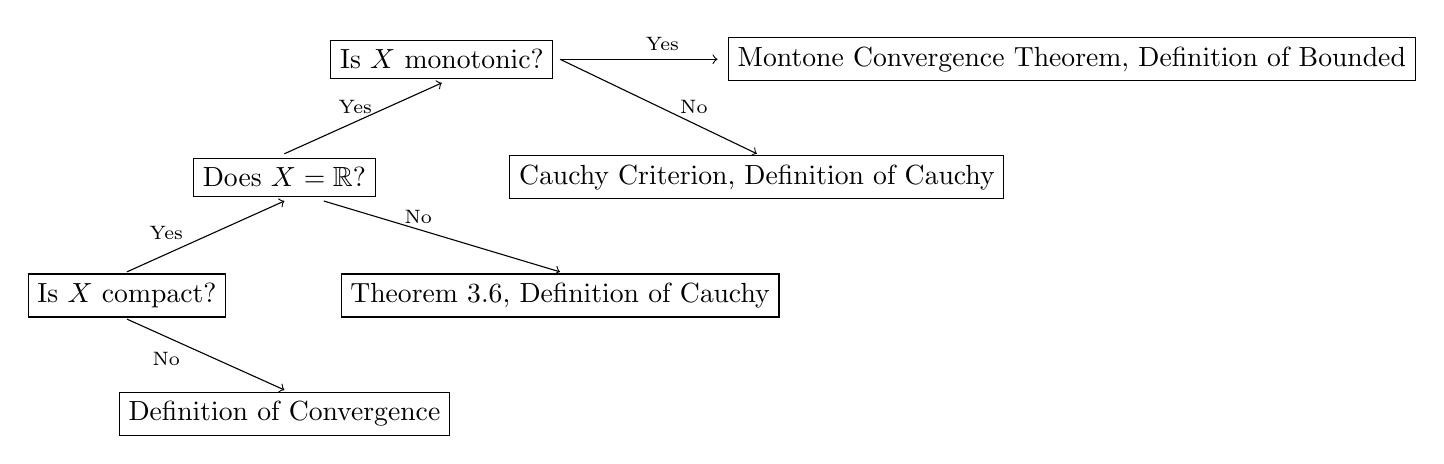
\begin{tikzpicture}
				\draw[->] (0,0.3)--(2,1.2);
				\draw[->] (2.5,1.2) -- (5.5,0.3);
				\draw[->] (0,-0.3)--(2,-1.2);
				\draw[->] (2,1.8) -- (4,2.7);
				\draw[->] (5.5,3)--(7.5,3);
				\draw[->] (5.5,3)--(8,1.8);
				\node[draw] at (0,0) {Is $ X $ compact?};
				\node[draw] at (2,1.5) {Does $ X=\R $?};
				\node[draw] at (2,-1.5) {Definition of Convergence};
				\node[draw] at (4,3) {Is $ X $ monotonic?};
				\node[draw] at (5.5,0) {Theorem 3.6, Definition of Cauchy};
				\node[draw] at (12,3) {Montone Convergence Theorem, Definition of Bounded};
				\node[draw] at (8,1.5) {Cauchy Criterion, Definition of Cauchy};
				\draw (0.5,0.8) node {\scriptsize Yes};
				\draw (0.5,-0.8) node {\scriptsize No};
				\draw (3.7,1) node {\scriptsize No};
				\draw (2.9,2.4) node {\scriptsize Yes};
				\draw (7.2,2.4) node {\scriptsize No};
				\draw (6.8,3.2) node {\scriptsize Yes};
			\end{tikzpicture}
			\caption{If $ \{x_n\} $ is a convergent sequence in $ X $, how do we prove that $ \{x_n\} $ converges?}
		\end{figure}
	\end{remark}
	\subsection{Sequences and Infinity}
	We have yet to discuss what happens when divergent sequences ``go off'' to infinity. 
	\begin{definition}\label{def}
		Let $ \{x_n\} $ be a sequence in $ \R $. If for all $ M\in\R $ there exists an $ N\in\N $ such that $ x_n\ge M $, we write $$\lim\limits_{n\to\infty}x_n=\infty .$$ Similarly, if for every $ M\in\R $ there exists an $ N\in\N $ such that $ n\ge N $ implies $ x_n\le M $, we write $$\lim\limits_{n\to\infty}x_n=-\infty .$$
	\end{definition}
	These definition make a slight abuse of notation, as they refer to the limit of a sequence despite the sequence in question diverging. 
	\begin{example}
		Let $ x_n=n $ be a sequence in $ \R $. For all $ M\in\R $, let $ N=M+1 $. We have $$s_n\ge s_{N}=N=M+1>M $$ for all $ n\ge N $. Therefore $ x_n\to\infty $.
	\end{example}
	\begin{remark}[Extended Real Numbers]
		If we were instead in the extended real numbers (Definition 1.19) $ \overline{\R} $, then the type of sequences given in Definition 3.10 would converge, because $ \{-\infty,\infty\}\subset\overline{\R} $. In fact, because every set in $ \overline{\R} $ is bounded, many of the results pertaining to sequences would be more general in $ \overline{\R} $. Any proposition or theorem that requires a sequence to be bounded in $ \R $, would not make this requirement in $ \overline{\R} $, as it would be implicitly met. 
	\end{remark}
	\subsection{$ \limsup $ and $ \liminf $}
	It can be insightful to study how the bounds of sequences change as $ n $ grows. For sequences in $ \R $, doing this illuminates interesting relationships between converge, bounds, limits of bounds, and subsequential limits. 
	
	A sequence is bounded if its range is a bounded set. If this sequence is in $ \R $, then we know something very powerful about the range of the sequence -- its supremum and infimum exist in $ \R $ (Theorem 1.2). The same can be said for the supremum and infimum of the set of all elements in the range of $ x_n $ that have yet to be realized, $\{x_m\mid m\ge n\} $. The set $ \{x_m\mid m\ge n\}$ is bounded above or below by $ x_n $, so the supremum or the infimum (or both) of $\{x_m\mid m\ge n\} $ exist. We will define the supremum and infimum of a set using this set of values $ \{x_m\mid m\ge n\} $. 
	\begin{definition}\label{def}
		Let $ x_n $ be a sequence in $ X $. The \textit{\color{red}infimum of a sequence } is $$ \inf x_n=\inf\limits_{m\ge n}x_m=\inf\{x_m\mid m\ge n\}.$$
	\end{definition}  
	\begin{definition}\label{def}
		Let $ x_n $ be a sequence in $ X $. The \textit{\color{red}supremum of a sequence} is $$ \sup x_n=\sup\limits_{m\ge n}x_m=\sup\{x_m\mid m\ge n\}.$$
	\end{definition}  
	The supremum and infimum of a sequence form their own sequences as the set $ \{x_m\mid m\ge n\} $ depends on the value of $ n $. Figure 36 illustrate the supremum and infimum of a sequence in $ \R $.
	\begin{figure}[h!]
		\centering
		\begin{tikzpicture}
			\draw (-.3,10) node {$ \R$};
			\draw (16,-0.3) node {$ \N$};		
			\draw[thick,->] (0,0) -- (0,10);
			\draw[thick,->] (0,0) -- (16,0);
			\draw [loosely dotted, ultra thick] (0,5) sin (0.5,10) cos (1,5) sin (1.5,1) cos (2,5) sin (2.5,9) cos (3,5) sin (3.5,2) cos (4,5) sin (4.5,8) cos (5,5) sin (5.5,3) cos (6,5) sin (6.5,7) cos (7,5) sin(7.5,4) cos (8,5) sin (8.5,6) cos (9,5) sin(9.5,4.5) cos (10,5) sin (10.5,5.25) cos(10.75,5) sin (11,4.75) cos (11.25,5) sin (11.5,5.25) cos(11.75,5) sin(12,4.75) cos(12.25,5) sin(12.5,5.25) cos(12.75,5)  sin(13,4.75) cos(13.25,5) sin(13.5,5.25) cos(13.75,5)  sin(14,4.75) cos(14.25,5) sin(14.5,5.25) cos(14.75,5);	
			\draw[loosely dotted, ultra thick, red] (0.5,10) -- (2.5,10);
			\draw[loosely dotted, ultra thick,red] (2.5,9) -- (4.5,9);
			\draw[loosely dotted, ultra thick,red] (4.5,8) -- (6.5,8);
			\draw[loosely dotted, ultra thick,red] (6.5,7) -- (8.5,7);
			\draw[loosely dotted, ultra thick,red] (8.5,6) -- (10.25,6);
			\draw[loosely dotted, ultra thick,red] (10.25,5.25) -- (14.75,5.25);
			\draw[loosely dotted, ultra thick, blue] (1.5,1) -- (3.5,1);
			\draw[loosely dotted, ultra thick,blue] (3.5,2) -- (5.5,2);
			\draw[loosely dotted, ultra thick,blue] (5.5,3) -- (7.5,3);
			\draw[loosely dotted, ultra thick,blue] (7.5,4) -- (9.5,4);
			\draw[loosely dotted, ultra thick,blue] (9.5,4.5) -- (10.5,4.5);
			\draw[loosely dotted, ultra thick,blue] (10.5,4.75) -- (15,4.75);
			\draw[loosely dotted, ultra thick,blue] (0,5) -- (1,5);
			\draw[loosely dotted,ultra thick,blue] (0.9,5) sin (1.4, 1);
			\draw[loosely dotted,ultra thick,red] (-0.1,5) sin (0.4, 10);
			\draw(5.5,5) node {$\{ x_n\}$};
			\draw[red] (5.5,8.3) node {$  \{\sup x_n\}$};
			\draw[blue] (6.5,2.6) node {$ \{\inf x_n\}$};
		\end{tikzpicture}
		\caption{A sequence $ \{x_n\} $ in $ \R $, with the sequence $ \{\sup x_n\} $ and $ \{\inf x_n\} $ shown in red and blue, respectively. For any $ n\in\N $, we take the supremum and infimum of all the points of $ \{x_m\mid m\ge n\}$. Graphically this means we take the supremum and infimum of all the points to the right of a certain value of $ \N $.  }
	\end{figure}
	\begin{example}
		Let $ x_n=1/n $ be a sequence in $ \R $. We have $ \{x_m\mid m\ge n\}=\{1/m \mid n\ge m\} $. This gives $ \sup x_n=1/n $ and $ \inf x_n=0 $, each being its own sequence in $ \R $.  
	\end{example}
	\begin{example}
		If $ x_n $ be a monotonically increasing sequence, then $ \inf x_n = x_n$ as $ x_n\le x_m $ for all $ m\ge n $. Similarly, if $ x_n $ is monotonically decreasing, then $ \sup x_n=x_n $.  
	\end{example}
	\begin{example}
		If $ x_n=\sin x $, then $ \inf x_n=-1 $ and $ \sup x_n=1 $ for all $ n\in\N $. 
	\end{example}
	Now we will define the limits of $ \sup x_n $ and $ \inf x_n$.
	\begin{definition}\label{def}
		Let $ \{x_n\} $ be a sequence in $ X $. The \textit{\color{red}limit inferior} of $ \{x_n\} $ is the limit of $ \{\inf x_n\} $, and is written as  $\liminf\limits_{n\to\infty} x_n$ or $\varliminf\limits_{n\to\infty} x_n. $ 
	\end{definition}
	\begin{definition}\label{def}
		Let $ \{x_n\} $ be a sequence in $ X $. The \textit{\color{red}limit superior} of $ \{x_n\} $ is the limit of $ \{\sup x_n\} $, and is written as  $\limsup\limits_{n\to\infty} x_n$ or $\varlimsup\limits_{n\to\infty} x_n. $ 
	\end{definition}
	\begin{example}
		The sequence $ x_n=1/n $ has a limit inferior of 0, and a limit superior of 0. 
	\end{example}
	\begin{example}
		The sequence $ x_n=\sin x $ has a limit inferior of -1, and a limit superior of 1. 
	\end{example}
	
	You may have noticed two things: the sequences $ \{\sup x_n\} $ and $ \{\inf x_n\} $ seem to always converge, and sometimes the limit inferior and limit superior are equal. The observations are consequences of our next results. 
	\begin{proposition}
		If $ \{x_n\} $ is a bounded sequence in $ \R $, then $ \liminf\limits_{n\to\infty} x_n $ and $ \limsup\limits_{n\to\infty} x_n $ exist. That is, the sequences $ \{\inf x_n\} $ and $ \{\sup x_n\} $ converge.
	\end{proposition} 
	\begin{proof}
		We will prove the result for the limit superior.\footnote{The proof for the limit inferior is very similar.} Let $ \{x_n\} $ be a bounded sequence in $ \R $. By the least-upper-bound property, $ \sup x_n $ exists for all $ n\in\N $, as the range of $ x_n $ is bounded. The sequence $ \sup x_n $ is bounded because $ x_n $ is bounded. By the Monotone Convergence Theorem, is suffices to show that $ \sup x_n $ is monotonically decreasing. We have $ \{x_n\mid m\ge n+1\}\subset \{x_n\mid m\ge n\} $, so any upper bound of $ \{x_n\mid m\ge n\} $ is an upper bound of  $ \{x_n\mid m\ge n+1\} $. This includes the least-upper-bound, which in this case is $ \sup x_n $. By the definition of the least-upper-bound, $ \sup x_{n+1} $ is less than all other upper-bounds of $ \{x_n\mid m\ge n+1\} $, therefore $ \sup x_n\ge \sup x_{n+1} $. This gives that $ \{\sup x_n\} $ is monotonically decreasing.   
	\end{proof}
	\begin{remark}[Monotonicity and Limits of Bounds]
		The proof of the last result took advantage of the fact that $ {\sup x_n} $ was monotonically decreasing and bounded, allowing the use of the Monotonic Convergence Theorem (Theorem 3.8). When we proved this result, we showed that a monotonically decreasing sequence will converge to its infimum. This means that $ \{\sup x_n\} $ converges to its infimum. For this reason the limit superior is sometimes written as $ \inf\sup x_n $. Similarly, the limit inferior can be written as $ \sup\inf x_n $. 
	\end{remark}
	\begin{proposition}
		Let $ \{x_n\} $ be a bound subsequence in $ \R $. Then 
		\begin{enumerate}
			\item There exist subsequences which converges to $ \limsup x_n $ and $ \liminf x_n $.
			\item For all $ c\in\R $, if there exists a subsequence which converges to $ c $, then $ \liminf x_n \le c\le \limsup x_n $. 
		\end{enumerate}
	\end{proposition}
	If we let $ E $ be the set of subsequential limits corresponding to a bounded $ \{x_n\} $ in $ \R $, then Proposition 3.6 concludes that $ \{\liminf x_n,\limsup x_n\}\subset E $, $ \liminf x_n=\inf E $, and $ \limsup x_n=\sup E $. 
	\begin{example}
		Let $ x_n=1/n $ be a sequence in $ \R $. It is convergent and bounded. We know from Example 3.37 that $ \liminf x_n=\limsup x_n=0 $. By Proposition 3.6, $ 0 $ is the only subsequential limit of $ \{x_n\} $. We already knew this though, because that is precisely what Theorem 3.3 asserts.
	\end{example}
	\begin{example}
		For $ x_n=\sin x $ in $ \R $, the set of subsequential limits is a subset of $ [-1,1] $. 
	\end{example}
	\begin{proposition}
		Let $ \{x_n\} $ be a bounded sequence in $ \R $. The sequence converges \textit{if and only if} $$ \liminf\limits_{n\to\infty} x_n=\limsup\limits_{n\to\infty} x_n.$$
	\end{proposition}
	\begin{proof}{\color{white}a}
		\begin{enumerate}
			\item [$ (\Longrightarrow) $] Suppose $ \{x_n\} $ converges to $ x\in \R $. By Theorem 3.3, every subsequence of $ \{x_n\} $ converges to $ x $. By Proposition 3.6, $ \lim\inf x_n $ and $ \limsup x_n $ are subsequential limits of $ \{x_n\} $. This means they both are $ x $, as $ x $ is the only subsequential limit of $ \{x_n\} $. Therefore $ \liminf x_n=\limsup x_n $.  
			\item [$ (\Longleftarrow) $] Assume that $ \limsup x_n=\liminf x_n=x $. For all $ \varepsilon>0 $, 
			\begin{align*}
				x-\varepsilon < \liminf x_n \le \limsup x_n< x+\varepsilon.
			\end{align*}
			This allows us to choose an $ N_1,N_2\in\N $ such that
			\begin{align*}
				s-\varepsilon<x_n<s+\varepsilon
			\end{align*}
			for all $ n\ge\max\{N_1,N_2\} $. This gives that $ |x_n-x|<\varepsilon $ for all such $ n $, so $ x_n\to x $. 
		\end{enumerate}
	\end{proof}
	\subsection{Series}
	Now we consider series. As we'll see, everything we did with sequences caries over nicely to series. In fact, working with series will be even simpler.
	
	A series is simply a special type of sequence which results from summing each element of a different sequence.
	\begin{definition}\label{def}
		Given a sequence $ \{x_n\} $ in a metric space $ X $, we have a \textit{\color{red}series} in the form of $$ \sum_{n=1}^{\infty}x_n. $$
	\end{definition}
	\begin{example}[Geometric Series]
		If we let $ x_n=1/2^n $, then $$ \sum_{n=1}^{\infty} \frac{1}{2^n}=\frac{1}{2}+\frac{1}{4}+\frac{1}{8}+\frac{1}{16}+\cdots .$$
	\end{example}
	In order to define the convergence of a series, we will look at the behavior of the first $ n $ terms. That is, we are interested in \begin{align*}
		s_1=\sum_{k=1}^{1}x_k&=x_1\\s_2=\sum_{k=1}^{2}x_k&=x_1+x_2\\s_3=\sum_{k=1}^{3}x_k&=x_1+x_2+x_3\\s_4=\sum_{k=1}^{4}x_k&=x_1+x_2+x_3+x_4\\&\vdots
	\end{align*} 
	If the sequence $ \{s_n\} $ converges, then we will say the series $ \sum_{n=1}^{\infty}x_n $ converges. 
	\begin{definition}\label{def}
		Let $ \sum_{n=1}^{\infty} x_n $ be a series in $ X $. Define the \textit{\color{red}partial sums} of the series to be the sequence $$ s_n=\sum_{k=1}^{n}x_k .$$ A series \textit{\color{red}converges} to $ x\in X $ if the sequence $ \{s_n\} $ converges to $ x\in X $. In this case, we write $$\sum_{n=1}^{\infty}x_n=x .$$
	\end{definition}
	
	\begin{remark}[Everything from Sequences Carries Over]
		Every single result we established for sequences can be formulated in terms of series, because every single series can be expressed as a sequence of partial sums. 
	\end{remark}
	Showing a series converges using this definition is unnecessarily difficult. In $ \R $ we can use a reformulation of the Cauchy Criterion
	\begin{theorem}[Cauchy Criterion for Series]
		Let $ \sum_{n=1}^{\infty}x_n $ be a sequence in $ \R $. The series converges \textit{if and only if} for all $ \varepsilon>0 $ there exists an $ N\in\N $ such that $$ \left\lvert\sum_{k=n}^{m}x_k \right\rvert\le\varepsilon $$ for all $ m\ge n \ge N $.
	\end{theorem}
	\begin{proof}
		This follows from the fact that $$ |s_n-s_m|=\left\lvert\sum_{k=1}^nx_n-\sum_{k=1}^mx_m  \right\rvert=\left\lvert\sum_{k=n}^{m}x_k \right\rvert .$$
	\end{proof}
	\begin{corollary}
		If $ \sum_{n=1}^\infty x_n $ converges, then $ x_n\to 0 $.
	\end{corollary}
	\begin{proof}
		Let $ m=n $ and use Theorem 3.9
	\end{proof}
	
	\begin{remark}[No Limit Needed!]
		Theorem 3.9 is a direct consequence of the Cauchy Criterion, so we don't need to know the limit of a convergent sequence to prove it converges. 
	\end{remark}
	\begin{example}
		The converse of Corollary 3.4 is not true! The harmonic series $ \sum_{n=1}^{\infty} 1/n$ diverges despite the fact that $ 1/n\to 0 $. 
	\end{example}
	
	
	\begin{example}
		The series $ \sum_{n}^{\infty}1/x! $ converges to $ e $ in $ \R $. This sequence does not converge in $ \Q $, as $ e\notin \Q $. 
	\end{example}
	\subsection{Tests for Convergent Series}
	Whenever we work with a series $ \sum_{n=1}^{\infty}x_n $, we want to find some way to relate a sequence involving $ x_n $ to the convergence of the series. There are three tests we can use to verify that a sequence in $ \R $ converges by doing just this: the comparison test, the ratio test, and the root test. Another benefit of these tests, is none require us to know the limit of a series to prove it converges! 
	\begin{theorem}[The Comparison Test]
		Let $ \sum_{n=1}^{\infty}x_n  $ be a series in $ \R $. If $ |x_n|\le y_n $ for $ n\ge N_0 $, where $ N_0 $ is some fixed integer, and if $ \sum_{n=1}^{\infty}c_n $ converges, then $ \sum_{n=1}^\infty x_n $ converges.
	\end{theorem}
	\begin{proof}
		For all $ \varepsilon>0 $, there exists an $ N\ge N_0 $ such that $ m\ge n\ge N $ implies $$ \sum_{k=n}^{m}y_k\le \varepsilon  ,$$ according to The Cauchy Criterion. Therefore we have $$ \left\lvert\sum_{k=n}^{m}x_k \right\rvert\le\sum_{k=n}^{m}|x_k|\le\sum_{k=n}^{m}y_k\le \varepsilon,  $$ so again by the Cauchy criterion, $\sum_{k=n}^{m}x_k  $ converges. 
	\end{proof}
	\begin{example}
		The geometric series $ \sum_{n=1}^{\infty}1/3^n $ converges to $ 3/2 $. We have $$\frac{1}{3^n+n}<\frac{1}{3^n} $$ for all $ n\in\N $, so the series $ \sum_{n=1}^{\infty}1/(3^n+n) $ converges by the Comparison Test.
	\end{example}
	\begin{example}
		The harmonic series $ \sum_{n=1}^{\infty}1/n  $ diverges. We have $$\frac{n}{n^2-\cos^2 n}>\frac{n^2}{n}=\frac{1}{n}.$$	Therefore by the converse of Theorem 3.10, the series $ \sum_{n=1}^{\infty}\frac{n}{n^2-\cos^2 n} $ diverges.
	\end{example}
	
	\begin{theorem}[The Ratio Test]
		If $ \sum_{n=1}^{\infty}x_n  $ is a series in $ \R $, then
		\begin{enumerate}
			\item the series converges if $ \lim_{n\to\infty}|x_{n+1}/x_n|<1 $;
			\item the series diverse if $ |x_{n+1}/x_n|\ge 1 $ for all $ n\ge N_0 $ for a fixed $ N_0\in\N $.
		\end{enumerate} 
	\end{theorem}
	\begin{proof}
		Suppose $ \lim |x_{n+1}/x_n|=\beta<1 $. For $ \varepsilon $ This means we can find an integer $ N\in\N $ such that $|x_{n+1}/x_n|<\beta $ for all $ n\ge N $. This can be rewritten as $ |x_{n+1}|<\beta|x_n| $. If we do this for $ n=N,N+1,N+2,\ldots ,N+k $, then \begin{align*}
			|x_{N+1}|&<\beta|x_N|,\\
			|x_{N+2}|&<\beta|x_{N+1}|<\beta^2|x_{N}|,\\
			&\vdots\\
			|x_{N+k}|&<\beta^p|a_N|.
		\end{align*}
		This gives $$ \sum_{k=N+1}^{\infty}|x_k|=\sum_{k=1}^{\infty}|x_{N+k}|<\sum_{k=1}^{\infty}\beta^k|x_N|=|x_N|\sum_{k=1}^\infty \beta ^k=|x_N|\frac{\beta}{1-\beta}.$$	Therefore by the Comparison Test, $ \sum_{n=1}^{\infty}x_k $ converges, because $$ \sum_{n=1}^{\infty}|x_n|\le\sum_{k=N+1}^{\infty}|x_k|.$$
		
		Now suppose that $ \limsup|x_{n+1}/x_n|=\beta>1 $. This means that $ |x_{n+1}|>|x_n| $ for a sufficiently large $ n $, meaning $ \lim\limits_{n\to\infty}x_n\neq 0 $. By the converse of Corollary 3.4, the series diverges.  
	\end{proof}
	\begin{example}
		Does $ \sum_{n=0}^{\infty}n!/5^n $ converge of diverge? 
		$$\lim\limits_{n\to\infty}\left\lvert \frac{x_{n+1}}{x_n}\right\rvert=\lim\limits_{n\to\infty}\left\lvert \frac{(n+1)!}{5^{n+1}}\frac{5^n}{n!}\right\rvert=\lim\limits_{n\to\infty}\frac{(n+1)!}{5n!}=\lim\limits_{n\to\infty}\frac{(n+1)n!}{5n!}=\lim\limits_{n\to\infty}\frac{n+1}{5}=\infty$$ By the Ratio Test, the series diverges. 
	\end{example}
	\begin{example}
		If we have $ \lim_{n\to\infty}|x_{n+1}/x_n|=1 $, then we aren't able to conclude anyhting about the convergence of a series. For example $ \sum_{n=1}^{\infty}1/n $ diverges, whereas  $ \sum_{n=1}^{\infty}1/n^2 $ converges. In both cases $ \lim_{n\to\infty}|x_{n+1}/x_n|=1 $. 	
	\end{example}
	\begin{theorem}[The Root Test]
		If $ \sum_{n=1}^{\infty}x_n  $ is a series in $ \R $, then
		\begin{enumerate}
			\item the series converges if $ \lim_{n\to\infty}\sqrt[n]{|x_n|}<1 $;
			\item the series diverges if $ \lim_{n\to\infty}\sqrt[n]{|x_n|}>1 $;
			\item we cannot determine anything if $ \lim_{n\to\infty}\sqrt[n]{|x_n|}=1 $.
		\end{enumerate} 
	\end{theorem}
	\begin{proof}
		Let $ \alpha=\lim_{n\to\infty}\sqrt[n]{|x_n|} $. If $ \alpha <1 $, we can find a $ \beta\in(\alpha,1) $, and an $ N\in\N $ such that $ \sqrt[n]{|x_n|}<\beta$ for $ n\ge N $. This inequality can be expressed as $ |x_n|<\beta^n $. Because $ \sum_{n=0}^{\infty}\beta^n $ converges, the Comparison Test gives that $\sum_{n=N}^\infty{|x_n|}$ converges. Since $$ \sum_{n=1}^\infty{|x_n|}=\sum_{n=N}^{N-1}{|x_n|}+\sum_{n=N}^\infty{|x_n|},$$ the series $ \sum_{n=1}^\infty{|x_n|} $ must converge, as the first sum is finite. 
		
		If $ \alpha>1 $, then $ |x_n|>1^n=1 $, so $ \lim\limits_{n\to\infty}x_n\neq 0 $. By Corollary 3.4, the series diverges.
		
		The series $ \sum_{n=1}^{\infty}1/n $ and $ \sum_{n=1}^{\infty}1/n^2 $ both have $ \alpha=1 $, despite the prior diverging and the latter converging. Therefore if $ \alpha=1 $, we cannot make any statement about convergence. 
	\end{proof}
	\begin{example}
		Does the series $\sum_{n=0}^{\infty}\left(\frac{5n-3n^3}{7n^3+3}\right)^n $ converge or diverge? 
		$$\lim\limits_{n\to\infty}\sqrt[n]{|x_n|}=\lim\limits_{n\to\infty}\left\lvert\left(\frac{5n-3n^2}{7n^3+2}\right)^n\right\rvert^{1/n} =\lim\limits_{n\to\infty}\left\lvert\frac{5n-3n^2}{7n^3+2}\right\rvert=\frac{3}{7}<1$$ By the Root Test, the series converges.
	\end{example}
	\begin{remark}[Slightly More General Tests]
		We can make the Ratio Test and Root Test a bit more powerful by using $ \limsup $ instead of just the limit. The proofs would be modified slightly. This will rarely make a difference. 
	\end{remark}
	\begin{remark}[Ratio vs. Root]
		The Ratio Test is much easier to use than the Root Test. Calculating ratios tends to be way easier than the $ n $th root of a value. That being said, the Root Test is more powerful in the sense that the Ratio Test will always agree with the Root Test. Furthermore, there are cases when the Ratio Test is inconclusive, but the Root Test is not. A good example of this is found in Example 3.35 in \cite{rudin1964principles}. 
	\end{remark}
	
	\subsection{Exercises}
	rudin, 3.4 part b
	
	constant sequences in $ \Z $
	
	subsequential limits closed
	
	series of nonnegative terms converges iff partial sums bounded
	\newpage
	\section{Continuity}
	We spent a fair amount of time studying what it means for a sequence or series to get ``arbitrarily close''to some point. We now want to do something similar with more general functions, and rigorously define continuity. Continuity makes nearly all of analysis possible, and without it we would be hopeless. Knowing the properties related to continuity will prove useful when proving many results, as many results will pertain exclusively to continuous functions. 
	\subsection{Limits of Functions}
	We begin by defining what a limit of a function is.
	\begin{definition}\label{def}
		Let $ X $ and $ Y $ be metric spaces, and $ E\subset X $. Suppose there is some function $ f:E\to Y $, and a limit point $ p $ of $ E $ and some $ L\in Y $ satisfying: for all $ \varepsilon>0 $ there exists a corresponding $ \delta>0 $ such that $d_Y(f(x),L)<\varepsilon $ for all points $ x\in E $ which satisfy $ d_X(x,p)<\delta $. We say that $ L $ is \textit{\color{red}the limit of $ f $ as $ x $ approaches p}, and write $$\lim\limits_{x\to p}f(x)=L .$$
	\end{definition} 
	This definition seems much more complicated than that given for convergence, but the concepts conveyed are fairly similar. It may be helpful to return to the somewhat lame example of playing a game with your friend involving $ \varepsilon $. Instead of a sequence you now play with some function $ f:E\to Y $, and a fixed limit point $ p\in E $.\footnote{It's important that $ p $ is a limit point. This means every neighborhood of $ p $ has infinitely many points, so we can always get arbitrarily close to it.} Your friend gives you a value of $ \varepsilon $, and he challanges you to find a $ \delta $ such that $ d_Y(f(x),L)<\varepsilon $ whenever $ d_X(p,x)<\delta $. Note that we never require that $ f(x)=L $ (see Figure 37). Our next several examples will make this more concrete.
	\begin{figure}[h!]
		\centering
		\begin{tikzpicture}
			\draw (-.3,9) node {$ \R$};
			\draw (16,-0.3) node {$ \R$};		
			\draw[thick,->] (0,0) -- (0,9);
			\draw[thick,->] (0,0) -- (16,0);
			\draw [blue, thick] plot [smooth, tension=1] coordinates { (1,1) (6,6) (14,9) };
			\draw[thick, dashed] (6,0) -- (6,6);
			\draw[thick, dashed] (5,0) -- (5,5.35);
			\draw[thick, dashed] (7,0) -- (7,6.55);
			\draw[thick, dashed] (0,6) -- (6,6);
			\draw[thick, dashed] (0,5.35) -- (5,5.35);
			\draw[thick, dashed] (0,6.55) -- (7,6.55);
			\filldraw[color=blue, fill=white] (6,6) circle (2pt);
			\filldraw[color=white, fill=blue] (6,2) circle (2pt);
			\draw (6,-0.3) node {$ x_0$};
			\draw (5,-0.3) node {$ x_0-\delta$};
			\draw (7,-0.3) node {$ x_0+\delta$};
			\draw[blue] (10,8.3) node {$ f(x)$};
			\draw (-0.9,5.35) node {$ L-\varepsilon$};
			\draw (-0.9,6.55) node {$ L+\varepsilon$};
			\draw (-0.8,6) node {$ L$};
		\end{tikzpicture}
		\caption{We have $ \lim_{x\to x_0}f(x)=L $ for a real function. No matter how small $\varepsilon $ gets, we can find a $ \delta $ such that $ |f(x)-L|<\varepsilon $ for all $ x $ satisfying $ |x-x_0|<\delta $. }
	\end{figure}
	\begin{example}
		Suppose we define $ f:\R\to\R $ as some linear function $ f(x)=mx+b $. For $ L=mx_0+b $ and $ x_0\in\R $, your friend gives you $ \varepsilon=0.1 $. You need to find a $ \delta $ such that $$d_\R(f(x),L)=|mx+b-(mx_0+b)|=|m(x-x_0)|=|m||x_0-x|<0.1.$$ Therfore you let $ \delta=0.1/|m| $. Instead of letting him keep naming $ \varepsilon $, you tell him that you'll just set $ \delta=\varepsilon/|m| $. This way whenever $ d_\R(f(x),L)<\varepsilon $ we have 
		$$ d_\R(f(x),L)=|mx+b-(mx_0+b)|=|m(x-x_0)|=|m||x_0-x|=|m|\cdot d_\R(x,x_0)<|m|\cdot\frac{\varepsilon}{|m|}=\varepsilon $$ whenever $ d_\R(x,x_0)<\delta $. Therefore $ \lim_{x\to x_0}f(x)=L $.  
	\end{example}
	\begin{example}
		Define $ f:\R\to\R $ as 
		$$ \begin{cases}
			1\text{ if }x>0\\-1\text{ if }x<0
		\end{cases} .$$
		We can show that the limit at $ x_0=0 $ fails to exist by finding one such $ \varepsilon $ where Definition 4.1 does not holds. Let $ \varepsilon=1/2 $, and suppose for contradiction $ \lim_{x\to x_0}f(x)=L $. We have that $ |f(x)-L|<\varepsilon=1/2 $ for all $ x $ such that $ |x-0|<\delta $. But we also have that 
		\begin{align*}
			2&=|1-(-1)|\\
			&=\left\lvert f(\delta/2)-f(-\delta/2) \right\rvert\\
			&=\left\lvert f(\delta/2)-L+L-f(-\delta/2) \right\rvert\\
			&\le\left\lvert f(\delta/2)-L|+|L-f(-\delta/2) \right\rvert\\
			&\le\frac{1}{2}+\frac{1}{2}\\&=1,
		\end{align*}
		which is a clear contradiction.
	\end{example}
	\begin{example}
		Suppose we define $ f:\R\to\R $ as $ f(x)=\sin x $. We can verify that $ \lim_{x\to 0}f(x)=1 $ despite the fact that $ f(x) $ is undefined at $ 0 $. If we let $ \delta=\sqrt{\varepsilon} $ and restrict our attention to the interval $ (-\pi/2,\pi/2) $,\footnote{This insures that $ 0<\cos x<\sin x/x <1 $.} then for all $ \varepsilon>0 $ we have $$d_\R(f(x),L)=\left\lvert \frac{\sin x}{x}-1\right\rvert<1-\cos x<2\sin^2\frac{x}{2}<\frac{x^2}{2}=\frac{|x-0|^2}{2}=\frac{d_\R(x,0)^2}{2}<\frac{(\sqrt{\varepsilon})^2}{2}<\varepsilon$$ whenever $ d_\R(x,0)<\delta $. 
	\end{example}
	As you may suspect, their is a very strong link between the convergence of a sequence and the limit of a function. If we have $ \lim_{x\to p}f(x)=L $, then $ p $ is a limit point of $ E\subset X $ as defined in Definition 4.1. This limiting process lets $ x $ become arbitrarily close to $ p $, much like a sequence would to its limit. As it turns out, there is a way to reformulate limits in terms of sequences if we use a sequence $ \{p_n\} $ in $ E $ which converges to $ p $.\footnote{Such a sequence is guaranteed to exist because $ p $ is a limit point of $ E $ (see Theorem 3.1).}
	\begin{theorem}
		Let $ X $ and $ Y $ be metric spaces, and $ E\subset X $. Suppose there is some function $ f:E\to Y $, and a limit point $ p $ of $ E $. Then $ \lim_{x\to p}f(x)=L $ \textit{if and only if} $ f(p_n)\to L $ (alternatively written as $ \lim_{n\to\infty}f(p_n)=L $) for every non-constant sequence $ \{p_n\} $ in $ E $ such that $ p_n\to p $.\footnote{The use of the same limit notation here may obscure the fact that $ \{f(p_n)\} $ is a sequence such that $ f(p_n)\to L $. } 
	\end{theorem} 
	\begin{proof}
		{\color{white}a}
		\begin{enumerate}
			\item [$ (\Longrightarrow) $] Suppose $ \lim_{x\to p}f(x)=L $. By Theorem 3.1, we can choose some arbitrary sequence $ \{p_n\} $ in $ E $ such that $ p_n\to p $. For all $ \varepsilon $ there exists a $ \delta>0 $ such that $ d_Y(f(x),L)<\varepsilon$ for all $ x\in E $ satisfying $ d_X(x,p)<\delta $. By the convergence of $ p_n $, there exists an $ N\in\N $ such that $ d_X(p_n,p)<\delta $ for all $ n>N $.\footnote{We take the $ \delta $ from the definition of a limit of a function and we use it as the $ \varepsilon $ in the definition of a limit of a sequence.} Therefore, for all $ n>N $, we have $d_Y(f(p_n),L)<\varepsilon$. This gives $$\lim_{n\to\infty}f(p_n)=L .$$
			\item [$ (\Longleftarrow) $] We will prove the contrapositive. Suppose that $ \lim_{x\to p}f(x)\neq L $. There exists some $ \varepsilon>0 $ such that for all $ \delta>0 $, there exists some point $ x\in E $ (which depends on $ \delta $) for which $ d_Y(f(x),L)\ge\varepsilon $ but $ d_X(x,p)<\delta $.\footnote{This is just the negation of Definition 4.1.} If we define $ \delta_n=1/n $ for all $ n\in\N $, then there is sequence $ \{p_n\} $ in $ E $ such that $ d(p_n,p)<\delta_n=1/n $. We have $ p_n\to p $ despite the fact that $ \lim_{n\to\infty}f(p_n)\neq L $. 
		\end{enumerate}
	\end{proof}
	\begin{example}
		For the real function $ f(x)=x $, it's clear that $ \lim_{x\to 0}f(x)=0 $. By Theorem 4.1 we know that $$ \lim\limits_{n\to\infty}f(1/n)=0,$$ as $ 1/n\to0 $. Furthermore we know this is the case for any $ \{x_n\} $ which converges to $ 0 $.  
	\end{example}
	So what's the big deal with writing limits in terms of sequences? This just seems like another complex relationship to remember. Theorem 4.1 is important because it allows us to prove many results involving limits (and later continuity) using properties we already know from sequences. For example, when using Theorem 4.1 we  know right away that limits of functions are unique because the limits of sequences are unique. 
	\begin{corollary}
		If $ f $ has a limit at $ p $, the limit is unique.
	\end{corollary}
	\begin{proof}
		If $ \lim_{x\to p}f(x)=L $, then by Theorem 4.1 the sequence $ \{f(p_n)\} $ converges to $ L $ for all $ \{p_n\} $ which converge to $ p $. By Proposition 3.2, $ L $ is unique. 
	\end{proof}
	The proof really amounts to nothing more than saying ``combine Theorem 4.1 and Proposition 3.2". We can combine Theorem 4.1 with Theorem 3.2 to arrive at familiar properties of functions. 
	\begin{theorem}
		Let $ X $ and $ Y $ be metric spaces, and $ E\subset X $. Suppose there are some functions $ f:E\to Y $ and $ g:E\to Y $, and a limit point $ p $ of $ E $. If $ \lim_{x\to p}f(x)=A $ and $ \lim_{x\to p}f(x)=B $, then
		\begin{enumerate}
			\item $ \lim_{x\to p}(f+g)(x)=A+B $;
			\item $ \lim_{x\to p}(fg)(x)=AB $;
			\item $ \lim_{x\to p}(f/g)(x)=A/B $ if $ B\neq 0 $.
		\end{enumerate}
	\end{theorem}
	\begin{proof}
		This follows from Theorem 4.1 and Theorem 3.2.
	\end{proof}
	\subsection{Continuous Functions}
	The definition of a limit of a function as given in Definition 4.1 has two quirks. The first, which has been acknowledged twice, is that a function needn't actually take on the value of its limit at a point. We never require $ f(p)=L $. Secondly, we do not require that $ p\in E $, we instead require that $ p $ is a limit point of $ p $. This means that not only can $ f $ be undefined at $ p $, but we shouldn't even be suprised that it is undefined at $ p $ when $ p\notin E $, as $ f:E\to Y $. We want to rule both of these out. Essentially, we want to define ``nice'' functions at a point $ p $ to be those where $ \lim_{x\to p}f(p)=L $. This is how we get our definition of continuity. 
	\begin{definition}\label{def}
		Let $ X $ and $ Y $ be metric spaces,  $ E\subset X $, $ p\in E $, and $ f:E\to Y $. Then $ f $ is \textit{\color{red}continuous at p} if for all $ \varepsilon>0 $, there exists a corresponding $ \delta>0 $ such that $$ d_Y(f(x),f(p))<\varepsilon $$ for all points $ x\in E $ which satisfy $ d_X(x,p)<\delta $. If $ f $ is continuous at every point of $ E $, then $ f $ is {\color{red}continuous (on $ E $)}. 
	\end{definition}
	This definition is illustrated in Figure 38. Just like in calculus, a function is continuous at a point $ x $ if and only if $$\lim\limits_{t\to x}f(t)=f(x) $$
	\begin{remark}
		Go back and review Remark 2.4. This issue came up with sequences. We saw sequences that converged in one metric space, but not another. Similarly, a function can be continuous in one metric space but not another. It also can be continuous on one subset of a metric space, but not another. If a subset $ E\subset X $ is never specified, then we assume that $ E=X $. This is why we usually consider all of $ \R $ when determining if a real function is continuous.
	\end{remark}
	\begin{figure}[h!]
		\centering
		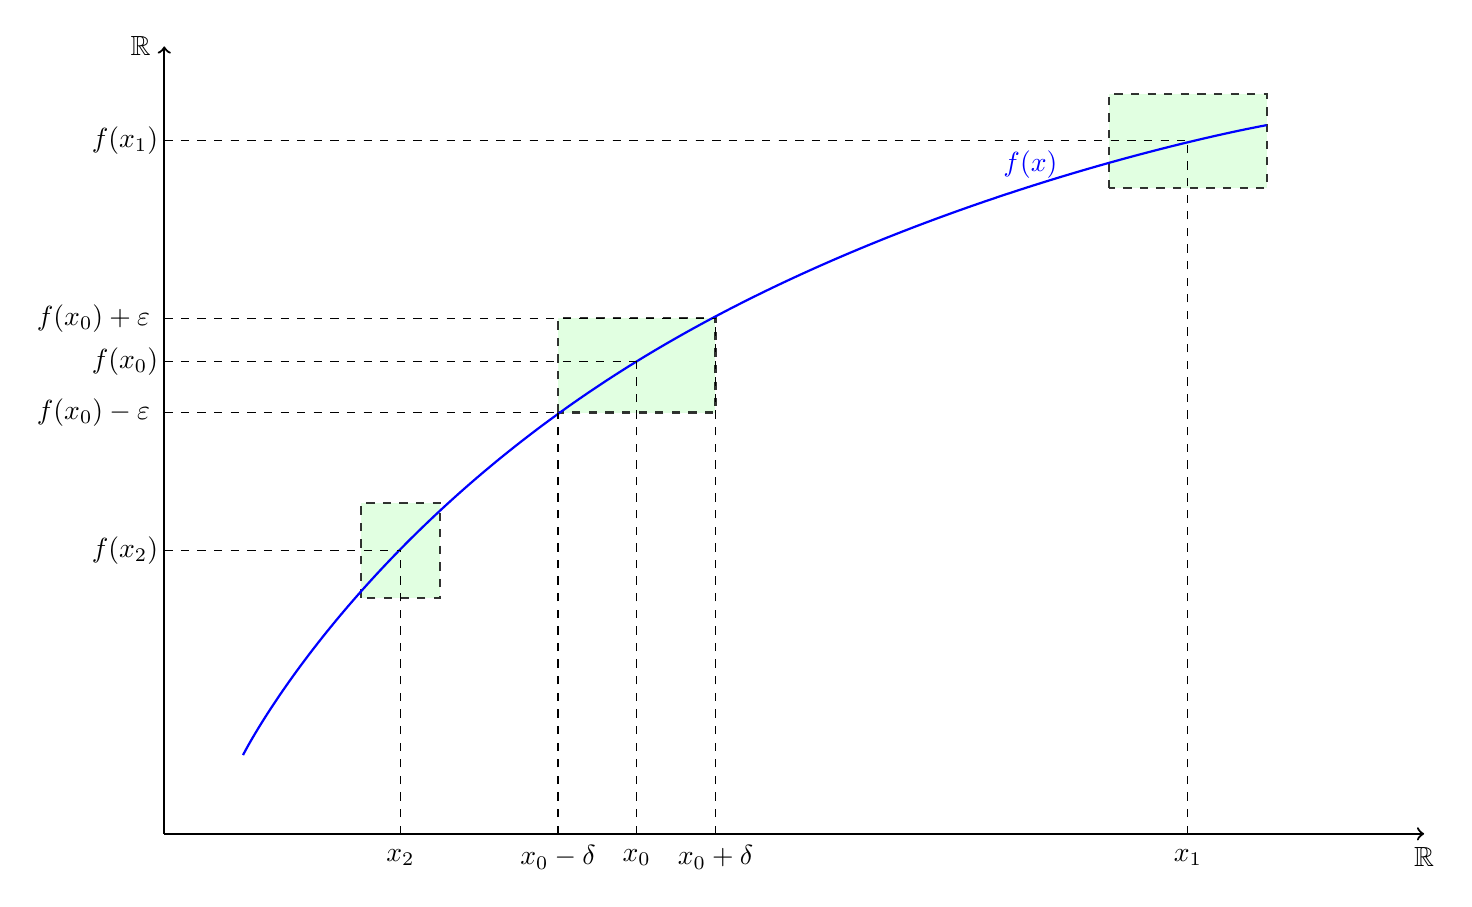
\begin{tikzpicture}
			\draw (-.3,10) node {$ \R$};
			\draw (-.5,8.8) node {$ f(x_1)$};
			\draw (16,-0.3) node {$ \R$};		
			\draw[thick,->] (0,0) -- (0,10);
			\draw[thick,->] (0,0) -- (16,0);	
			\draw[fill=green!15, thick, dashed, opacity=0.8] (5,5.35) rectangle (7,6.55);
			\draw[fill=green!15, thick, dashed, opacity=0.8] (12,8.2) rectangle (14,9.4);
			\draw[fill=green!15, thick, dashed, opacity=0.8] (2.5,3) rectangle (3.5,4.2);
			\draw [blue, thick] plot [smooth, tension=1] coordinates { (1,1) (6,6) (14,9) };
			\draw[thin, dashed] (6,0) -- (6,6);
			\draw[thin, dashed] (5,0) -- (5,5.35);
			\draw[thin, dashed] (7,0) -- (7,6.55);
			\draw (13,-0.3) node {$ x_1$};
			\draw[thin, dashed] (0,6) -- (6,6);
			\draw[thin, dashed] (0,5.35) -- (5,5.35);
			\draw[thin, dashed] (0,6.55) -- (7,6.55);
			\draw (6,-0.3) node {$ x_0$};
			\draw (5,-0.3) node {$ x_0-\delta$};
			\draw (7,-0.3) node {$ x_0+\delta$};
			\draw[blue] (11,8.5) node {$ f(x)$};
			\draw (-0.9,5.35) node {$ f(x_0)-\varepsilon$};
			\draw (-0.9,6.55) node {$ f(x_0)+\varepsilon$};
			\draw (-0.5,6) node {$ f(x_0)$};
			\draw[thin, dashed] (13,0) -- (13,8.75);
			\draw[thin, dashed] (0,8.8) -- (13,8.8);
			\draw[thin, dashed] (0,8.8) -- (13,8.8);
			\draw[thin, dashed] (3,0) -- (3,3.6);
			\draw[thin, dashed] (0,3.6) -- (3,3.6);
			\draw (-.5,3.6) node {$ f(x_2)$};
			\draw (3,-0.3) node {$ x_2$};
		\end{tikzpicture}
		\caption{The function $ f $ is continuous at $ x_0 $, $ x_1 $, and $ x_2 $. Given some $ \varepsilon>0 $, there exist a delta such that $ |f(x)-f(y)|<\varepsilon $ for all $ |x-y|<\delta $. Each green box has height of $ 2\varepsilon $, and the width for the $ 2\delta $ at the corresponding point. Note that the value of $ \delta $ is the same for $ x_0 $ and $ x_1 $, but different for $ x_2 $. For a fixed $ \varepsilon $, the delta for one point may differ depending on the value of $ x $. If some value of $ \delta $ is too large, then the box would be too wide, and the function $ f(x) $ would ``escape'' from the top and/or bottom of the box. This graphical feature would imply a violation of continuity, so we need to shrink $ \delta $ until the function ``escapes'' from the sides (which is what we did for $ x_2 $).   }
	\end{figure}
	\begin{example}
		Suppose we define $ f:\R\to\R $ as some linear function $ f(x)=mx+b $. Let $ p\in\R $. We can mimic our work in Example 4.1 to show this function is continuous on all of $ \R $. For $ p\in\R $ satisfying $ |x-p|<\varepsilon/|m| $, we have$$ d_\R(f(x),f(p)=|mx+b-(my+b)|=|m(x-p)|=|m||x-p|=|m|\cdot d_\R(x,p)<|m|\cdot\frac{\varepsilon}{|m|}=\varepsilon .$$ Therefore $ f $ is continuous at $ p $, for all $ p\in\R $
	\end{example}
	\begin{example}
		Let $ f:\R\to\R $ be define as $$ \begin{cases}
			1\text{ if }x>0\\-1\text{ if }x\le0
		\end{cases} .$$
		This function is continuous on the set $ \R\backslash\{0\} $. It fails to be continuous on all of $ \R $, as there is a ``jump'' from $ -1 $ to $ 1 $ at $ x=0 $. 	
	\end{example}
	\begin{example}
		The function $ f:\R\to\R $ defined as $ f(x)=x^2 $ is continuous on $ \R $. Let $ p\in\R $. For all $ \varepsilon>0 $, define $ \delta=\min\{1,\varepsilon/(2|p|+1)\} $. We have $$|f(x)-f(p)|=|x^2-p^2|=|x-p|\cdot|x+p|<\delta(2|p|+1)=\varepsilon ,$$ for $ x\in \R $ which satisfy $ |x-p|<\delta $.  Therefore $ f $ is continuous at $ p $, for all $ p\in\R $. 
	\end{example}
	\begin{example}[Thomae's function]
		Define the real function $ f:[0,1]\to[0,1] $ as $$f(x)=\begin{cases}
			\frac{1}{q} \text{ if }x=\frac{p}{q}\text{ for }p,q\in\Z\\
			0\text{ if }x\notin\Q
		\end{cases} ,$$ where we assume $ p/q\in\Q $ is in simplest terms. The function $ f $ is continuous for the irrational numbers in $ [0,1] $ but discontinues for the rational numbers in $ [0,1] $. 
		
		Suppose $ r\in[0,1] $ is irrational, giving $ f(r)=0 $. Fix $ \varepsilon>0 $. By the Archimedean Property, there is some $ m\in\N $ such that $ 1/m \varepsilon$, and some $ k_m\in $ such that $$ r\in\left(\frac{k_m}{m},\frac{k+1}{m}\right) .$$ Define the following values:
		\begin{align*}
			d_m&=\min\left\{\left\lvert r-\frac{k}{m}\right\rvert,\left\lvert r-\frac{k+1}{m}\right\rvert\right\},\\
			&\delta=\min\{d_1,\ldots,d_m\}.
		\end{align*}
		If $ x\in[0,1] $ is a rational number with $ |x-r|<\delta $, then $ x=p/q $ and $ q>m $, so $$|f(x)-f(r)|=\left\lvert \frac{1}{q}-0\right\rvert=\frac{1}{q}<\frac{1}{m}<\varepsilon ,$$ whenever $ |x-r|<\delta $. If $ x\in[0,1] $ is irrational, then $$ |f(x)-f(r)|=|0-0|=0<\varepsilon ,$$ regardless of $ \delta $. Thus, for any $ x\in[0,1] $ satisfying $ |x-r|<\delta $, $ |f(x)-f(r)|<\varepsilon $. The function is continuous at any irrational $ r $.
		
		Now suppose $ r=p/q\in[0,1] $ is rational. We have $ f(r)=1/q $. Let $ \varepsilon=1/2q $ and define $ r_k=r+\frac{1}{k\sqrt{2}} $. The number $ r_k $ is irrational, so $ f(r_k)=0 $. Can we find a $ \delta $ such that $$ |f(x)-f(r)|=\left\lvert f(x)-\frac{1}{q}\right\rvert<\varepsilon=\frac{1}{2q}?$$ No we cannot. We can always find and $ x_k $ such that $$|f(x_k)-f(r)|=\frac{1}{q}>\frac{1}{2q}. $$  
	\end{example}
	\begin{remark}[Pathological Examples]
		Thomae's function is constructed for the express purpose of being an unintuitive example. Such examples are known as pathological in math, and are particularly common in analysis. While such examples would never arise in the real world, they often give insight into just what is possible. We'll see several more: a function that is continuous everywhere but differentiable nowhere, a set that we can not possible know the size of, a set that is uncountably infinite but has no size, etc. 
	\end{remark}
	\begin{remark}[Can $\delta  $ depend on $p $?]
		Yes! In Example 4.5, our selection of $ \delta $ was independent of $ x $, and works for every point in $ \R $. This was not the case for Example 4.7, but that is fine. Our selection of $ \delta $ will change for each value of $ p\in\R $. All that matters is \textit{for each} $ \varepsilon>0 $, we can find a correspond $ \delta $. We'll come back to this idea shortly.  
	\end{remark}
	\begin{remark}[It Only Takes One $ \varepsilon $, Discontinuity]
		Showing a function is \textit{not} continuous only requires we find a single $ \varepsilon $ such that $ |f(x)-f(y)|\ge\varepsilon $ for all $ |x-y|<\delta $ for $ y\in E $. This follows from the negation of Definition 4.1. If we let $ x\to0 $, then we end up with $ \delta=0 $, a clear contradiction. 
	\end{remark}
	Our next makes explicit the fact that if $ f $ is continuous at a point, then the limit of the function exists at that point.
	\begin{theorem}
		Let $ X $ and $ Y $ be metric spaces,  $ E\subset X $, $ p \in E $ be a limit point of $ E $, and $ f:E\to Y $. Then $ f $ is continuous \textit{if and only if} $ \lim_{x\to p}f(x)=f(p) $.
	\end{theorem}
	\begin{proof}
		Simply compare the definition of a limit (Definition 4.1), with the definition of continuity (Definition 4.2).
	\end{proof}
	\begin{corollary}[Continuous Functions Preserve Limits]
		Let $ X $ and $ Y $ be metric spaces, and $ E\subset X $. Suppose there is some function $ f:E\to Y $, and a $ p\in E $ which is a limit point of $ E $. Then $ f $ is continuous at $ p $ \textit{if and only if} $ f(p_n)\to f(p) $ for every non-constant sequence $ \{p_n\} $ in $ E $ such that $ p_n\to p $. That is $$\lim\limits_{n\to \infty}f(p_n)=f\left(\lim\limits_{n\to\infty} p_n\right)=f(p) .$$
	\end{corollary}
	\begin{proof}
		This follows from Theorem 4.1 and Theorem 4.3. 
	\end{proof}
	\begin{corollary}[Properties of Continuous Functions] 
		Let $ X $ and $ Y $ be metric spaces, and $ E\subset X $. Suppose there are some functions $ f:E\to Y $ and $ g:E\to Y $, and a point $ p \in E $. If $ f $ and $ g $ are continuous at $ p $, then 
		\begin{enumerate}
			\item $ f+g $ is continuous at $ p $;
			\item $ fg $ is continuous at $ p $;
			\item $ f/g $ is continuous at $ p $ if $ p\neq0 $.
		\end{enumerate}
	\end{corollary}
	\begin{proof}
		This follows from Theorem 4.2 and Theorem 4.3.
	\end{proof}
	\begin{remark}[Moving Around Limits]
		Corollary 4.2 is the first time we've encountered a type of question analysis will provide answers for again and again -- when can I move a limit into a function/operation? The majority of Section 7 will be dedicated to these type of questions. Corollary 4.2 tells us that a function is continuous if and only if the limit of a function is the function of the limits.   
	\end{remark}
	\begin{figure}[h!]
		\centering
		\begin{tikzpicture}
			\draw (-.3,10) node {$ \R$};
			\draw (-.5,8.23) node {$ f(p)$};
			\draw (14,-0.3) node {$ \R$};		
			\draw[thick,->] (0,0) -- (0,10);
			\draw[thick,->] (0,0) -- (14,0);
			\draw[thick,dashed, ->] (1,-1) -- (11,-1);	
			\draw[thick,dashed, ->] (-1.3,1) -- (-1.3,8.23);
			\draw[blue] (12,9) node {$ f(x)$};
			\draw [blue, thick] plot [smooth, tension=1] coordinates { (1,1) (6,6) (14,9) };
			\draw[thick, dashed] (11,0) -- (11,8.23);
			\draw[thick, dashed] (0,8.23) -- (11,8.23);
			\draw[ultra thin, dashed] (0,1) -- (1,1) -- (1,0);
			\draw[ultra thin, dashed] (0,2.5) -- (2,2.5) -- (2,0);
			\draw[ultra thin, dashed] (0,3.6) -- (3,3.6) -- (3,0);
			\draw[ultra thin, dashed] (0,4.5) -- (4,4.5) -- (4,0);
			\draw[ultra thin, dashed] (0,5.3) -- (5,5.3) -- (5,0);
			\draw[ultra thin, dashed] (0,6) -- (6,6) -- (6,0);
			\draw[ultra thin, dashed] (0,6.6) -- (7,6.6) -- (7,0);
			\draw[ultra thin, dashed] (0,7) -- (8,7) -- (8,0);
			\draw[ultra thin, dashed] (0,7.5) -- (9,7.5) -- (9,0);
			\draw[ultra thin, dashed] (0,7.9) -- (10,7.9) -- (10,0);
			\draw (11,-0.3) node {$ p$};
			\draw (6,-1.3) node {$ p_n\to p$};
			\draw (1,-0.3) node {\tiny $ p_1$};
			\draw (2,-0.3) node {\tiny $ p_2$};
			\draw (3,-0.3) node {\tiny $ p_4$};
			\draw (4,-0.3) node {\tiny $ p_8$};
			\draw (5,-0.3) node {\tiny $ p_{16}$};
			\draw (6,-0.3) node {\tiny $ p_{32}$};
			\draw (7,-0.3) node {\tiny $ p_{64}$};
			\draw (8,-0.3) node {\tiny $ p_{128}$};
			\draw (9,-0.3) node {\tiny $ p_{256}$};
			\draw (10,-0.3) node {\tiny $ p_{512}$};
			\draw (-.5,1) node {\tiny$ f(p_1)$};
			\draw (-.5,2.5) node {\tiny$ f(p_{2})$};
			\draw (-.5,3.6) node {\tiny$ f(p_{4})$};
			\draw (-.5,4.5) node {\tiny$ f(p_{8})$};
			\draw (-.5,5.3) node {\tiny$ f(p_{16})$};
			\draw (-.5,6) node {\tiny$ f(p_{32})$};
			\draw (-.5,6.6) node {\tiny$ f(p_{64})$};
			\draw (-.5,7) node {\tiny$ f(p_{128})$};
			\draw (-.5,7.5) node {\tiny$ f(p_{256})$};
			\draw (-.5,7.9) node {\tiny$ f(p_{512})$};
			\draw (-2.5,4.165) node {$ f(p_{n})\to f(p)$};
		\end{tikzpicture}
		\caption{For $ p_n\to p $, we have $ f(p_n)\to f(p) $, therefore $ f $ is continuous at $ p $. }
	\end{figure}
	\begin{example}
		Define $ f:\R\to\R $ as $$\begin{cases}x\text{ if }x\in\Q\\ 0\text{ if }x\notin\Q\end{cases}. $$ This function is continuous at $ 0 $, because for all real $ x_n\to 0 $, $ f(x_n)\to f(0)=0 $. This happens to be the only point in $ \R $ at which $ f $ is continuous. Let $ c\in\Q\backslash\{0\} $. There is a sequence of irrational numbers $ \{x_n\} $ such that $ x_n\to c $. Despite this, $ f(x_n)=0\to0\neq c $, so $ f $ is not continuous at $ c $. Similarly, if $ c\in\R\backslash\Q $, then there exists a sequence of rationals $ x_n $ such that $ x_n\to c $. Despite this, $ f(x_n)=x_n\to c\neq f(c)=0 $, so $ f $ is not continuous at $ c $. 
	\end{example}
	While Corollary 4.3 proves valuable when showing a function is continuous, when combined with our next result, we can show that almost any function we can write down is continuous.  
	\begin{theorem}[Composition Preserves Continuity]
		Let $ X $, $ Y $, and $ Z $ be metric spaces, and $ E\subset X $. If $ f:E\to Y $ and $ g:f(E)\to Y $ are continuous at $ p\in E $ and $ f(p)\in f(E) $ respectively, then the function $ h:g(f(E))\to Z $ defined as  $$ h(x)=g(f(x))=(g\circ f)(x)$$ is continuous at $ p $. 
	\end{theorem}
	\begin{proof}
		Fix $ \varepsilon>0 $. Since $ g $ is continuous at $ f(p) $, there exists a $ \delta' $ such that $$d_Z(g(y),g(f(p))<\varepsilon $$ if $ d_Y(y,f(p))<\delta' $ for $ y\in f(E) $. Since $ f $ is continuous at $ p $, there exists $ \delta>0 $ such that $$d_Y(f(x),f(p))<\delta' $$ if $ d_X(x,p)<\delta $ and $ x\in E $.\footnote{We took the $ \delta' $ from the definition of $ g $'s continuity, and let $ \varepsilon=\delta' $ for the definition of $ f $'s continuity. This means that any $ f(x) $ which satisfy $ d_Y(f(x),f(p))<\delta'  $ will satisfy $ d_Y(y,f(p))<\delta' $.} These inequalities give $$d_Z(g(f(x)),g(f(p)))=d_Z(h(x),h(p))<\varepsilon $$ if $ d_X(x,p)<\delta $ and $ x\in E $. Therefore $ h=g\circ f $ is continuous at $ p $. 
	\end{proof}
	If $ h=g\circ f $ is continuous, then any composition of $ h $ with another continuous function will also be continuous. If we keep composing the result with continuous functions, we will always have a continuous function. For this reason, nearly every function encountered in actual applications will be continuous.   
	\begin{example}
		Let $ f:\R\to\R $ be defined as $$ f(x)=\left(\frac{e^{\sin x}}{\cos x}\right)^4 .$$ If we let $ g(x)=\cos x $, $ h(x)=\sin  x $, $ j(x)=e^x $, $ k(x)=x^4 $ (all continuous functions from $ \R $ to $ \R $), then $$f(x)=k\circ((j\circ h)/g).$$ By Theorem 4.4 and Corollary 4.3, $ f(x) $ is continuous. 
	\end{example}
	If a continuous function is a ``nice'' mapping from some metric space $ E\subset X $ to another metric space $ Y $, it's worth asking what happens to sets when they mapped using $ f $? If $ E $ is open, will the image $ f(E) $ be open? Does this hold for closed sets? What about our favorite sets, compact sets? We will now begin to put continuity in conversation with Section 2, and the point-set topology of metric spaces. We'll end this subsection by introducing a \textit{very important} theorem related to the topology of a metric space. We will then introduce a special type of continuity, before seeing how continuity interacts with compactness.
	\begin{theorem}
		Let $ X $ and $ Y $ be metric spaces. The function $ f:X\to Y $ is continuous on $ X $ \textit{if and only if} $ f^{-1}(V) $ is open in $ X $ for every open set $ V $ in $ Y $.
	\end{theorem}
	\begin{proof}
		{\color{white}a}
		\begin{enumerate}
			\item [$ (\Longrightarrow) $] Suppose $ f $ is continuous on $ X $ and $ V$ is an open set in $ Y $. We need to show that $ f^{-1}(V) $ is open by showing every point of the set is an interior point. Let $ p\in f^{-1}(V)\subset X $, and $ f(p)\in V $. The set $ V $ is open, so there exists an $ r=\varepsilon>0 $ such that $ N_\varepsilon(f(p))\subset V $. Alternatively we may write, $ y\in V $ for all $ d_Y(f(p),y)<\varepsilon $. The function $ f $ is continuous at $ p $ because $ p\in X $, so there exists a $ \delta>0 $ such that $ d_Y(f(x),f(p))<\varepsilon $ is $ d_X(x,p)<\delta $. In terms of sets, this means that $ N_\delta(p)\subset f^{-1}(V) $, so $ p\in f^{-1}(V) $ is an interior point. Therefore $ f^{-1}(V) $ is open.
			\item [$ (\Longleftarrow) $] Suppose $ f^{-1}(V) $ is open in $ X $ for all open sets $ V $ in $ Y $. For $ p\subset X $ and $ \varepsilon>0 $, let $ V=N_\varepsilon(f(p)) $. Alternatively, $ V $ is the set of all $ y $ such that $ d_Y(y,f(p))<\varepsilon $. The set $ V $ is a neighborhood, so it is open, hence $ f^{-1}(V) $ is open. If $ f^{-1}(V) $ is open, then there exists a $ \delta $ such that $ N_\delta(p)\subset f^{-1}(V) $. In other words, as soon as $ d_X(p,x)<\delta $, $ x\in f^{-1}(V) $. Because $ x\in f^{-1}(V) $, $ f(x)\in f(V) $, so we have $ d_Y(f(x),f(p))<\varepsilon $ as soon as $ d_X(p,x)<\delta $. This means $ f $ is continuous on $ X $. =
		\end{enumerate}
	\end{proof}
	\begin{corollary}
		Let $ X $ and $ Y $ be metric spaces. The function $ f:X\to Y $ is continuous on $ X $ \textit{if and only if} $ f^{-1}(V) $ is closed in $ X $ for every closed set $ V $ in $ Y $.
	\end{corollary}
	\begin{proof}
		The complement of an open set is closed, and $ f^{-1}(V^c)=(f^{-1}(V))^c $. 
	\end{proof}
	Theorem 4.5 is illustrated in Figure 40 for a real function. 
	\begin{remark}[Topological Definition of Continuity]
		We've already referenced several times the fact that we are restricting our attention to metric spaces, but that point-set topology can be studied in a more general setting. As it turns out, when working in a topological space that is not a metric space, we define a continuous function as one with the property established in Theorem 4.5. If you were to ever take a proper topology course, continuity is never discussed in terms of $ \varepsilon-\delta $, but is instead related to open sets.
	\end{remark}
	\begin{figure}[h!]
		\centering
		\begin{tikzpicture}
			\draw (-.3,10) node {$ \R$};
			\draw (14,-0.3) node {$ \R$};		
			\draw[thick,->] (0,0) -- (0,10);
			\draw[thick,->] (0,0) -- (14,0);
			\draw[blue] (12,9) node {$ f(x)$};
			\draw [blue, thick] plot [smooth, tension=1] coordinates { (1,1) (6,6) (14,9) };
			\draw[ultra thin, dashed] (0,2.5) -- (2,2.5) -- (2,0);
			\draw[ultra thin, dashed] (0,6.6) -- (7,6.6) -- (7,0);
			\draw[ultra thick,red] (2,0) -- (7,0);
			\draw[ultra thick,red] (0,2.5) -- (0,6.6);
			\filldraw[color=red, fill=white] (2,0) circle (2pt);
			\filldraw[color=red, fill=white] (7,0) circle (2pt);
			\filldraw[color=red, fill=white] (0,2.5) circle (2pt);
			\filldraw[color=red, fill=white] (0,6.6) circle (2pt);
			\draw[red] (-0.4,4.55) node {$ V $};
			\draw[red] (4.5,-0.4) node {$ f^{-1}(V) $};
		\end{tikzpicture}
		\caption{A continuous function $ f:\R\to\R $, and the open interval $ V\subset \R $. Because $ f $ is continuous, $ f^{-1}(V) $ is open in $ \R $. }
	\end{figure}
	\begin{example}
		Theorem 4.5 only says that the preimage of an open set will be open when a function is continuous. It never says that the image of and open set is open. If we define $ f:\R\to\R $ as $ f(x)^2 $, and let $ E=(-1,1) $ be an open set, then $$f(E)=[0,1) .$$ Therefore $ f(E) $ is not open, despite $ f $ being continuous on $ \R $. 
	\end{example}
	\begin{example}
		Theorem 4.5 greatly simplifies the proof of Theorem 4.4. For an open $ E\subset Z $, $ g^{-1}(E)\subset Y $ is open by the continuity of $ g $. The set $ f^{-1}(g^{-1}(E))\subset X $ is open because $ f $ is continuous. Therefore, for $ h=g(f(x)) $, $ h^{-1}(E)\subset X $ is open, making $ h $ continuous. 
	\end{example}
	\subsection{Uniform Continuity}
	Before exploring compactness and continuity, we need to address an earlier remark, namely Remark 4.3. We noticed that the value of $ \delta $ which corresponds to $ \varepsilon $ sometimes depends on where we are in the domain of a function. While does not violate continuity, it is a bit odd. If $ f $ is continuous on a set $ E $, then we can always find a corresponding $ \delta $ for each $ \varepsilon $, but that $ \delta $ may not work for all values of $ E $. What we are really doing is find a corresponding $ \delta $ for each $ \varepsilon $ \textit{and} for each $ p\in E $. However, Example 4.5 showed us that sometimes our corresponding $ \delta $ works \textit{for all} values on the domain. This is a special case that merits its own definition. 
	\begin{definition}\label{def}
		Let $ X $ and $ Y $ be metric spaces. The function $ f:X\to Y $ is \textit{\color{red}uniformly continuous (on $ X $)} if for every $ \varepsilon>0 $, there exists a $ \delta>0 $ such that $d_X(x,p)<\delta $ implies $  d_Y(f(x),f(p))<\varepsilon$ \textit{for all} $ x,p\in X $. 
	\end{definition}
	There are two major differences between uniform continuity and continuity. We already discussed the first -- we find a single value $ \delta $ which works for all elements of $ f $'s domain. This difference arises from the fact that in Definition 4.2, we only looked at $ p\in E $ which satisfy $ d_X(x,p)<\delta $. We don't do this in definition 4.3, as we look at \textit{all} $ p\in E $. The second is that uniform continuity pertains to sets, not points. While a function can be continuous at a single point, saying $ f $ is uniformly continuous at a point it vacuously true and meaningless, as the concept deals with multiple points in a domain. It also should be clear that any function which is uniformly continuous is continuous. 
	
	It cannot be emphasized enough how much stronger uniform continuity is than continuity. If $ f:\R\to\R $ is continuous, then for every $ \varepsilon>0 $ (of which there are an uncountably infinite amount), we may need to find a corresponding $ \delta $ for each point in $ \R $! It is feasible that we have an uncountably infinite amount of $ \delta $ for each $ \varepsilon $. If instead $ f $ is uniformly continuous, for each fixed $ \varepsilon>0 $ (of which there are still an uncountably infinite amount), then we know there is one ``silver bullet'' $ \delta $ that works for all of $ \R $. This difference gives rise to an interesting geometric interpretation presented in Figure 41 and Figure 42. 
	\begin{figure}[h!]
		\centering
		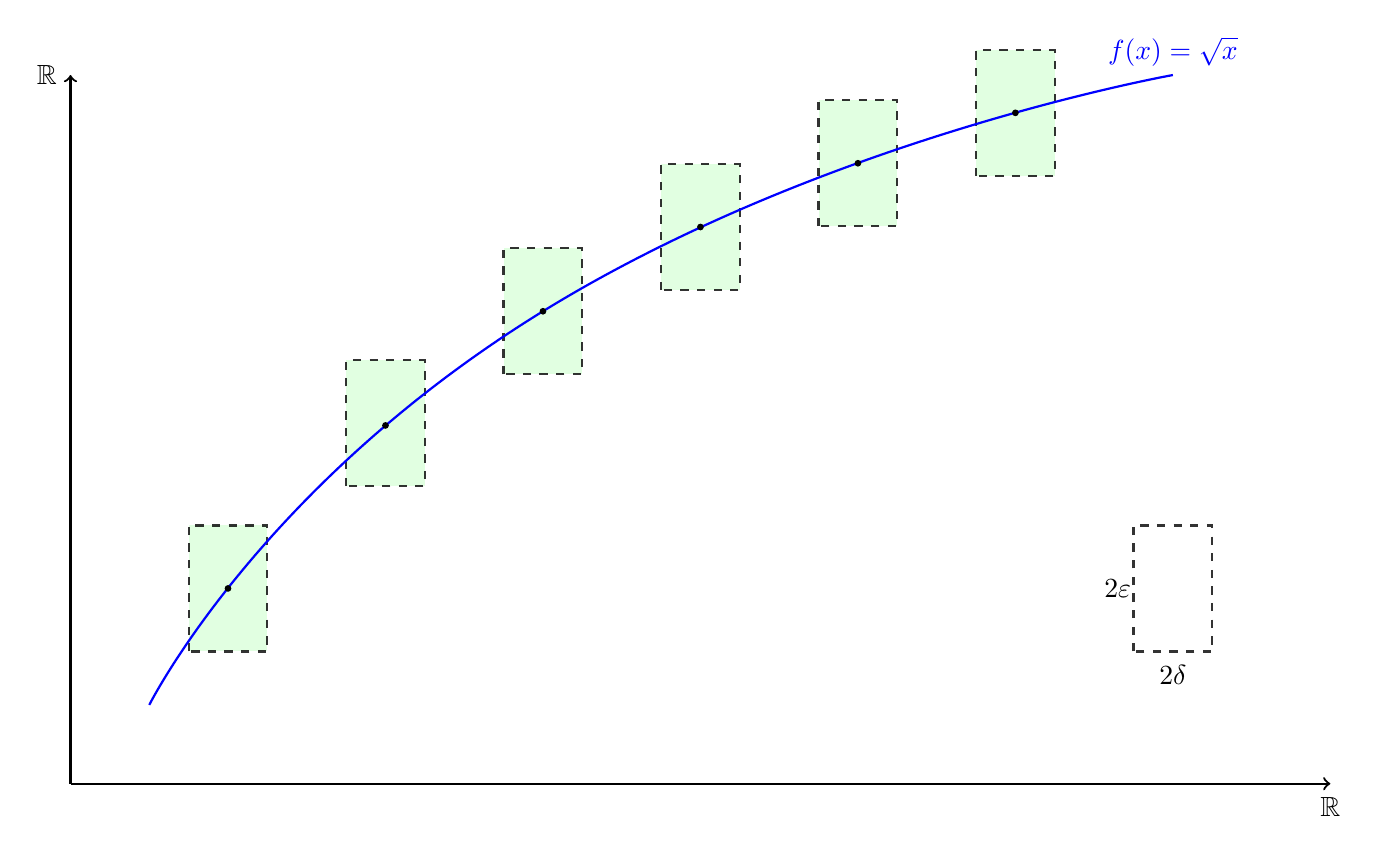
\begin{tikzpicture}
			\draw (-.3,9) node {$ \R$};
			\draw (16,-0.3) node {$ \R$};		
			\draw[thick,->] (0,0) -- (0,9);
			\draw[thick,->] (0,0) -- (16,0);
			\draw[fill=green!15, thick, dashed, opacity=0.8] (1.5,1.68) rectangle (2.5,3.28);
			\draw[thick, dashed, opacity=0.8] (13.5,1.68) rectangle (14.5,3.28);
			\draw[fill=green!15, thick, dashed, opacity=0.8] (3.5,3.78) rectangle (4.5,5.38);
			\draw[fill=green!15, thick, dashed, opacity=0.8] (5.5,5.2) rectangle (6.5,6.8);
			\draw[fill=green!15, thick, dashed, opacity=0.8] (7.5,6.27) rectangle (8.5,7.87);
			\draw[fill=green!15, thick, dashed, opacity=0.8] (9.5,7.08) rectangle (10.5,8.68);
			\draw[fill=green!15, thick, dashed, opacity=0.8] (11.5,7.72) rectangle (12.5,9.32);
			\draw [blue, thick] plot [smooth, tension=1] coordinates { (1,1) (6,6) (14,9)};
			\filldraw (4,4.55) circle (1pt);
			\filldraw (2,2.48) circle (1pt);
			\filldraw (6,6) circle (1pt);
			\filldraw (8,7.07) circle (1pt);
			\filldraw (10,7.88) circle (1pt);
			\filldraw (12,8.52) circle (1pt);
			\draw[blue] (14,9.3) node {$ f(x)=\sqrt{x}$};
			\draw[black] (13.3,2.48) node {$ 2\varepsilon$};
			\draw[black] (14,1.38) node {$ 2\delta$};
		\end{tikzpicture}
		\caption{Let $ f:(0,1]\to\R $ be defined as $ f(x)=\sqrt{x} $. The function is uniformly continuous. For each fixed $ \varepsilon $, we can center a box of height $ \varepsilon $ at a point $ (x,f(x)) $. We can find some width of the box $ \delta $ such that the function will never ``escape'' from the top or bottom of the box, no matter the point $ (x,f(x)) $.}
	\end{figure}
	\begin{figure}[h!]
		\centering
		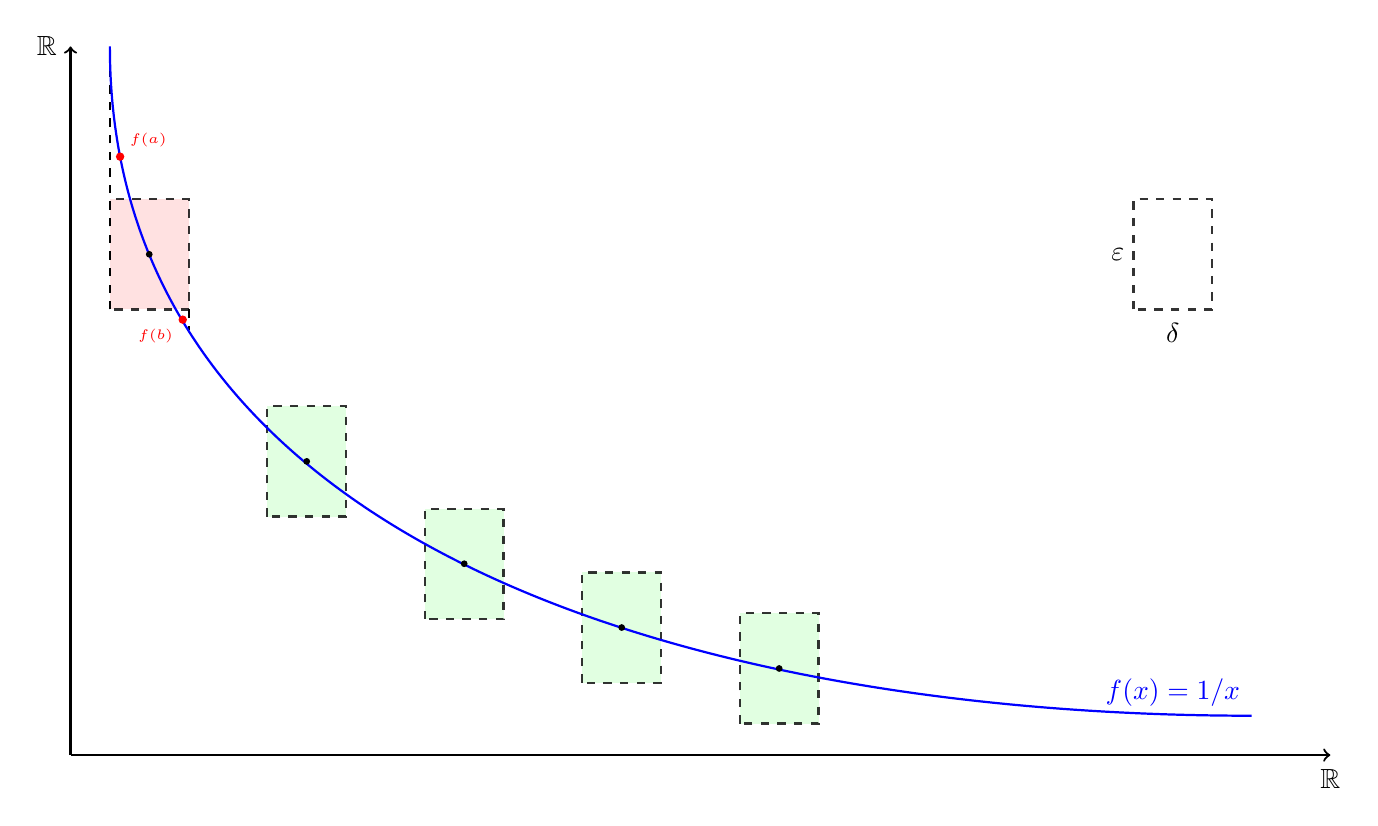
\begin{tikzpicture}
			\draw (-.3,9) node {$ \R$};
			\draw (16,-0.3) node {$ \R$};		
			\draw[thick,->] (0,0) -- (0,9);
			\draw[thick,->] (0,0) -- (16,0);
			\draw[fill=red!15, thick, dashed, opacity=0.8] (0.5,5.66) rectangle (1.5,7.06);
			\draw[fill=green!15, thick, dashed, opacity=0.8] (2.5,3.03) rectangle (3.5,4.43);
			\draw[fill=green!15, thick, dashed, opacity=0.8] (4.5,1.73) rectangle (5.5,3.13);
			\draw[fill=green!15, thick, dashed, opacity=0.8] (6.5,.92) rectangle (7.5,2.32);
			\draw[fill=green!15, thick, dashed, opacity=0.8] (8.5,.4) rectangle (9.5,1.8);
			\draw[thick, dashed] (0.5,5.66) -- (0.5,9);
			\draw[thick, dashed] (1.5,5.66) -- (1.5,5.4);
			\draw[ thick, blue]   (0.5,9) to[out=270,in=180] (15,0.5);
			\draw[blue] (14,0.8) node {$ f(x)=1/x$};
			\filldraw (1,6.36) circle (1pt);
			\filldraw (3,3.73) circle (1pt);
			\filldraw (5,2.43) circle (1pt);
			\filldraw (7,1.62) circle (1pt);
			\filldraw (9,1.1) circle (1pt);
			\draw[thick, dashed, opacity=0.8] (13.5,5.66) rectangle (14.5,7.06);
			\draw[black] (13.3,6.36) node {$ \varepsilon$};
			\draw[black] (14,5.36) node {$ \delta$};
			\filldraw[red] (0.63,7.6) circle (1.3pt) node [anchor= south west] {\tiny$ f(a) $};
			\filldraw[red] (1.425,5.53) circle (1.3pt) node [anchor= north east] {\tiny$ f(b) $};
		\end{tikzpicture}
		\caption{The function $ f:\R\to\R $ defined as $ f(x)=1/x $ is not uniformly continuous. For our set value of $ \varepsilon $ and $ \delta $ the function ``escapes'' from the top and bottom of the red rectangle. This is because there exists $ a,b\in\R $ such that $ |f(a)-f(b)|\ge\varepsilon $ despite the fact that $ |a-b|<\delta $. We could make the corresponding $ \delta $ smaller, but the function eventually ``escape'' as we move to the left. }
	\end{figure}
	\begin{example}
		Let $ f:[0,\infty)\to\R $ be defined as $ f(x)=\sqrt{x} $. The function is uniformly continuous on $ [0,\infty) $. If we let $ \delta=\varepsilon^2 $, then for all $ |x-p|<\delta $, we have $$|f(x)-f(p)|^2=|\sqrt{x}-\sqrt{p}|^2\le|\sqrt{x}-\sqrt{p}|\cdot|\sqrt{x}+\sqrt{p}|=|x-p|<\varepsilon^2 .$$ Taking the square root of this inequality gives $ |f(x)-f(p)|<\varepsilon $ for all $ |x-p|<\delta $. Our choice of $ \delta $ does not depend on $ p\in\R $, so $ f $ is uniformly continuous. 
	\end{example}
	\begin{example}
		The function $ f:\R\to\R $ defined as $ f(x)=1/x $ is not uniformly continuous on $ (0,1] $. Suppose for contradiction that $ f $ is uniformly continuous on $ (0,1) $. Let $ \varepsilon=1/n $. There exists a $ \delta $ such that $$ |f(x)-f(p)|=\left\lvert\frac{1}{x}-\frac{1}{p}\right\rvert=\left\lvert\frac{x-p}{xp}\right\rvert<\frac{\delta}{xp}<\varepsilon=\frac{1}{n} $$ for all $ x,p\in(0,1) $ satisfying $ |x-p|<\delta $. Therefore we need $ \delta<|xp|/n $ for all $ x,y\in(0,1) $ satisfying $ |x-p|<\delta $. If we let $ y=x+\delta/2 $, then $ \delta<|xp|/n $ becomes $$\delta <\frac{2x^2}{2n-x} $$ for all $ x\in(0,1) $. 
	\end{example}
	\subsection{Continuity and Compactness}
	If continuous functions are ``nice'', and compact sets are ``nice'', then it should not come as a surprise that continuous functions behave very well with compact sets. We will first define what it means for a function to be bounded, and then we will jump into a series of results about compactness.
	\begin{definition}\label{def}
		Let $ E\subset\R $. The real function $ f:E\to\R $ is \textit{\color{red}bounded} if there exists an $ M\in f(x) $ such that $ |f(x)|\le M $ for all $ x\in E $.
	\end{definition}
	Figure 43 shows a bounded real function.
	\begin{figure}[h!]
		\centering
		\begin{tikzpicture}
			\draw (-.3,10) node {$ \R$};
			\draw (16,4.7) node {$ \R$};		
			\draw[thick,->] (0,0) -- (0,10);
			\draw[thick,dashed] (0,9.5) -- (15,9.5);
			\draw[thick,dashed] (0,0.5) -- (15,0.5);
			\draw[thick,->] (0,5) -- (16,5);	
			\draw [thick, blue] (1,6) sin (5,9) cos (9,5) sin (14,1);
			\draw[thick] (1,4.8) -- (1,5.2);
			\draw[thick] (14,4.8) -- (14,5.2);
			\draw[black] (1,4.5) node {$ a $};
			\draw[black] (-.3,9.5) node {$ M $};
			\draw[black] (-.4,0.5) node {$ -M $};
			\draw[black] (14,4.5) node {$ b $};
			\filldraw[blue] (1,6) circle (2pt);
			\filldraw[blue] (14,1) circle (2pt);
		\end{tikzpicture}
		\caption{A bounded function $ f:[a,b]\to\R $ }
	\end{figure}
	\begin{example}
		The function $ \sin (x) $ is bounded on all of $ \R $, as $ |\sin x|\le 1 $ for all $ x\in\R $.
	\end{example}
	\begin{example}
		The function $ f(x)=x^2 $ on $ \R $ is continuous but not bounded. 
	\end{example}
	\begin{theorem}[Continuity Preserves Compactness]
		Let $ f:X\to Y $ be a continuous function where $ X $ and $ Y $ are metric spaces. If $ X $ is compact, then $ f(X) $ is compact. 
	\end{theorem}
	\begin{proof}
		We will show that an arbitrary open cover $ \{V_\alpha\} $ of $ f(X) $ has a finite subcover. Since $ f $ is continuous, $ f^{-1}(V_\alpha) $ is open for all $ \alpha $ (Theorem 4.5). The set $ X $ is compact, so there exists finitely many indices $ \alpha_1,\ldots,\alpha_n $ such that $$X\subset f^{-1}(V_{\alpha_1})\cup\ldots\cup f^{-1}(V_{\alpha_n}) .$$ But we have $ f(f^{-1})(E)\subset E $ for any $ E\subset Y $, so we can take the image of the finite subcover of $ X $ and conclude $$ f(X)\subset V_{\alpha_1}\cup\ldots\cup V_{\alpha_n} .$$ Therefore $ f(X) $ is compact. 
	\end{proof}
	This result is similar to Theorem 4.5, but they ``go in different directions''. The preimage of an open set is open for a continuous $ f $. Now we are saying that the image of a compact set is compact for a continuous $ f $. It's tempting to say this holds for open sets, but it is not true. In general openness is not preserved by continuous functions (Example 4.11).
	\begin{corollary}
		Let $ E\subset\R $. If the real function $ f:E\to\R $ is continuous and $ E $ is closed and bounded, then $ f(E) $ is closed and bounded.
	\end{corollary}
	\begin{example}
		Let $ f:(0,\infty)\to\R $ be the continuous function $ f(x)=1/x $. The set $ (1,\infty) $ is neither closed nor bounded, so $ f^{-1}((1,\infty))=(0,1) $ is neither closed nor bounded. 
	\end{example}
	Our next theorem proves useful in many applications, as it allows us to determine when a function has a maximum and minimum on an intervals. 
	\begin{theorem}[Extreme Value Theorem]
		Suppose $ f $ is a continuous real function on a compact metric space $ X $, and \begin{align*}
			M&=\sup\limits_{x\in X}f(x),\\
			m&=\inf\limits_{x\in X}f(x).
		\end{align*}
		Then there exists points $ x,y\in X $ such that $ f(x)=M $ and $ f(y)=m $.
	\end{theorem}
	\begin{proof}
		Continuous functions preserve compactness (Theorem 4.6), so $ f(X)\subset\R $ is closed and bounded. A closed and bounded set contain their infimum and supremum, so $ f(X) $ contains $ M $ and $ m $. 
	\end{proof}
	\begin{remark}[$ \sup $ or $ \max $?]
		It may not be clear when we use maximum and when we use supremum. A maximum of some set or function is always attained. This is not always the case for a supremum. If we know that $ \sup E\in E $, then we are free to write $ \max E=\sup E $, but this won't always hold. For instance, $ (0,1) $ has a supremum of $ 1 $, but no well defined maximum. If you're ever unsure if the supremum is attained in the set or by the function, use $ \sup $. A maximum is always a supremum, so it technically is not incorrect. The same holds for $ \inf $ and $ \min $.
	\end{remark}
	Theorem 4.7 tells us that if a function is defined on a compact space, then it \textit{must} achieve a maximum and minimum on that domain. Just knowing that such points exist is a great deal of information. 
	\begin{example}
		The function $ \sin(x) $ does not achieve a maximum or minimum on the interval $ (0,\pi/2) $, despite it being bounded. We can always find some larger value of $ f(x) $ as we get arbitrarily close to $ \pi/2 $, or some smaller value of $ f(x) $ as we get arbitraily close to $ 0 $. This is the exact type of behavior we ruled out when defining compactness! By defining $ \sin(x) $ on $ [0,\pi/2] $, we now achieve a maximum and minimum on the interval.  
	\end{example}
	\begin{example}
		The function $ f(x)=x^2 $ achieves a minimum on $ \R $, but it fails to achieve both a maximum and a minimum on all of $ \R $. This is because $ \R $ is neither closed nor bounded, rendering it not compact. 
	\end{example}
	Recall the fact that $ f(x)=1/x $ is not uniformly continuous on $ (0,1) $. In Figure 42 we argued that no matter the value of $ \delta $ given for a fixed $ \varepsilon $, we could move the rectangle of height $ \varepsilon $ and length $ \delta $ to the left until the function ``escaped'' from the top and bottom. Us being able to keep moving the rectangle to the left is a result of $ (0,1) $ not being closed. We can always get a little bit closer to $ 0 $ without leaving the domain. As we do this, the function will take on larger values indefinitely because $ f((0,1))=(1,\infty) $ is unbounded. These two observations seem to hint at the fact that if eliminate these behaviors, a function will always be uniformly continuous. As it turns out, compactness does just this, and the proof of this is one of the more elegant proofs in analysis.\footnote{Full disclosure: this is my favorite proof from basic real analysis.} 
	\begin{theorem}
		Let $ f $ be a continuous function which maps a compact metric space $ X $ to a metric space $ Y $. Then $ f $ is uniformly continuous on $ X $.
	\end{theorem}
	\begin{proof}
		Fix $ \varepsilon>0 $. The function $ f $ is continuous on $ X $, so for each point $ p\in X $ there is a $ \delta(p) $ such that $$d_Y(f(p),f(x))<\varepsilon/2 $$ whenever $ x\in X $ and $ d_X(p,x)<\frac{1}{2}\delta(p) $.\footnote{We are writing $ \delta $ as a function of $ p\in X $ to emphasize that all we know now if $ f $ is continuous.} Let $$ J(p)=\left\{x\in X \mid d_X(x,p)<\frac{1}{2}\delta(p)\right\} .$$ We have $ p\in J(p) $ for all $ p\in X $, so $$X\subset\bigcup_{p\in X}J(p),$$ where $ J(p) $ is open for all $ p\in X $.\footnote{This follows from the fact that $ J(p) $ is a neighborhood of $ p $, and all neighborhoods are open sets. We could also write $ J(p)=N_{1/2\delta(p)}(p) $.} That is to say, $ \{J(p)\}_{p\in X} $ is an open cover of $ X $. The space $ X $ is compact, so there exists a finite set of points $ p_1,\ldots,p_n $ such that $$ X\subset J(p_1)\cup\cdots\cup J(p_n).$$ If we let $$ \delta=\frac{1}{2}\min\{\delta(p_1),\ldots,\delta(p_n)\},$$ then $ \delta>0 $.\footnote{This finite set achieves is infimum so we use $ \min $. A minimum of a finite set of positive numbers in positive. This is not necessarily the case with an infimum of an infinite set of positive numbers even if that set is compact. For us to be able to conclude $ \delta>0 $, it is crucial that the set $ \{\delta(p_1),\ldots,\delta(p_n)\} $ is finite, that way we can take the minimum over a finite set corresponding to the finite subcover. }
		
		Let $ x,p\in X $ such that $ d_X(x,p)<\delta $. The point $ p $ is in $ X $, so it must be ``covered'' by one of the open sets in the finite subcover $ \{J(p_1),\ldots,J(p_n)\} $. That is, there is an $ m\in\N $, where $ 1\le m\le n $, such that $ p\in J(p_m) $. Hence, $d_X(x,p_m)<\frac{1}{2}\delta(p_m) $. The triangle inequality gives $$d_X(x,p_m)\le d_X(x,p)+d_X(p,p_m)<\delta+\frac{1}{2}\delta(p_m)\le\delta(p_m) .$$ But then, we can use the triangle inequality and the continuity of $ f $ to conclude $$d_Y(f(x),f(p))\le d_Y(f(x),f(p_m))+d_Y(f(p_m),f(p))<\frac{\varepsilon}{2}+\frac{\varepsilon}{2}=\varepsilon ,$$ so $ f $ is uniformly continuous.
	\end{proof}
	This proof may look technical, but the underlying idea is much simpler. Think about the function $ f(x)=1/x $ on $ (0,1] $, and Figure 42. For a fixed $ \varepsilon $, we can always move the rectangles to the left until the function ``escapes'' from the top or bottom. The closer we get to $ 0 $ on the $ x -$axis, the smaller we need to make $ \delta $, and we can always move closer and closer to $ 0 $, so there isn't one $ \delta $ that will work at every point. Suppose instead we looked at $ f(x)=1/x $ on the interval $ [0.001,1] $. We may be able to get closer and closer to $ 0.001 $, making $ \delta $ smaller as we go to satisfy continuity, but because $ 0.001 $ is defined by $ f $, we could just take the $ \delta $ that works at $ 0.001 $ and use it for all of $ [0.001,1] $. If the $ \delta $ needs to become small as we move our rectangle to the left, then the ``leftmost'' point must have the smallest $ \delta $, a choice of $ \delta $ that will work for all of $ [0.001,1] $ and our fixed $ \varepsilon $. The next example will walk through this process, and the proof of Theorem 4.8, with an actual function. 
	\begin{example}
		Suppose $ f:[-10,10]\to\R $ is defined as $ f(x)=x^2 $. Example 4.7 showed that $ f $ is continuous. In this case we had $ \delta=\min\{1,\varepsilon/(2|p|+1)\} $. Fix $ \varepsilon=1 $, so $ \varepsilon/2=1/2 $.\footnote{We use $ \varepsilon=1 $ as the final value of $ \varepsilon $ used to show uniform continuity. The value $ \varepsilon/2 $ is used in the definition of continuity of $ x^2 $.} We can let $ \delta(p)=1/(4|p|+1) $, and have $$|f(x)-f(p)|<\varepsilon=1/2 $$ for all $ p\in [-10,10] $ satisfying $ |x-p|<\frac{1}{2}\delta(p)<\delta(p) $. First, we should explicitly show that $ \delta(p) $ will change with $ p $. Suppose $ p=1 $, giving $ \delta(1)=1/5 $. For all $ x\in[-10,10] $ such that $ |x-1|<1/5 $, we do indeed have $ |x^2-1|<1/2 $. Now let's try to use $ \delta(1) $ for $ p=9 $. The set of all $ x\in[-10,10] $ which satisfy $ |x-9|<1/5 $ is $ (44/5,46/5) $. For $ 91/10\in(44/5,46/5) $, we have $$ |f(91/10)-f(9)|=\left(\frac{91}{10}\right)^2-9^2=1.81>\frac{1}{2}=\frac{\varepsilon}{2}.$$ This means that $ \delta(1) $ won't work for $ p=9 $! We now will mimic the proof of Theorem 4.8 and find a $ \delta $ that will work for all $ p\in[-10,10] $. 
		
		Define $$J(p)=\left\{x\in[-10,10]\ \Big|\  |x-p|<\frac{1}{2}\delta(p)=\frac{1}{8|p|+2}\right\}=N_{1/2\delta(p)}=N_{1/(8|p|+2)}(p). $$ We have $ p\in J(p) $ for all $ p\in[-10,10] $, so $$ [-10,10]\subset\bigcup_{p\in [-10,10]}J(p) .$$ For the finite set of points $ P=\{-10,-9.9,\ldots,9.9,10\}=\{-10+(0.1)n\mid n=1,\ldots, 200\} $,\footnote{Where the heck do I get this set? Well the minimum value of $ 1/(8|p|+2) $ on the interval $ [-10,10] $ is about 0.012. If we round this down to 0.01, then all the $ J(p) $ centered at points in $ [-10,10] $ that are distance 0.01 apart will be guaranteed to cover $ [-10,10] $, as we took the distance between points to be less than the smallest radius of $ J(p) $. } we have $$ [-10,10]\subset\bigcup_{p\in P}J(p) ,$$ making $ \{J(p)\}_{p\in P} $ a finite subscover of $ [-10,10] $. Define $$ \delta=\min\limits_{p\in P}\{\delta(p)\}=\delta(10)=\delta(-10)=\frac{1}{81} .$$
		
		We will show that this value of $ \delta $ will work for a random point in $ [-10,10] $, say $ p=1.95 $. We could verify this right away, but we'll instead follow the steps of the proof, even though they become painfully redundant when working with actual numbers.  Now let $ x\in[-10,10] $ such that $ |x-1.95|<1/81 $.\footnote{For the rest of this paragraph, whenever we refer to $ x $, we mean these particular $ x $ satisfying  $ |x-1.95|<1/81 $} We have $ x\in[-10,10] $, so it must be in one of the elements of the finite subcover $ \{J(p)\}_{p\in P} $. We in fact have $ 1.95\in J(1.9) $, hence $$ |1.95-1.9|<\frac{1}{2}\delta(1.95)=0.0581 ,$$so the continuity of $ f $ at $ p=1.95 $ gives
		\begin{align}
			|f(1.95)-f(1.9)|=0.1925<\frac{\varepsilon}{2}=\frac{1}{2}.
		\end{align}
		We also have $$|x-1.9|\le|1.95-x|+|1.95-1.9|<\delta+\frac{1}{2}\delta(1.95)=\frac{1}{81}+0.0581=0.0704<\delta(1.95)=.104,  $$ so by the continuity of $ f $ at $ 1.9 $, 
		\begin{align}
			|f(x)-1.9|<\frac{\varepsilon}{2}=\frac{1}{2}.
		\end{align}
		Combining Equation (5) and (6)	gives $$|f(x)-f(1.95)|\le|f(x)-f(1.9)|+|f(1.9)-f(1.95)|<\frac{1}{2}+\frac{1}{2}=1=\varepsilon $$ for all $ x\in[-10,10] $ such that $ |x-1.95|<\delta=1/81 $. Our choice of $ \delta $ does in fact work for $ \varepsilon=1 $ and $ p=1.95 $! 
		
		The choice of $ p=1.95 $ does not matter. We could have picked \textit{any} value in $ [-10,10] $, and $ \delta=1/81 $ still would have worked for $ \varepsilon=1 $. This should not come as a surprise, because we just picked \textit{one of} the smallest value of $ \delta(p) $ for $ p\in[-10,10] $. Why is it that we need compactness if we could have just let $ \delta=\min_{p\in[-10,10]}\delta(p) $? This would work in this specific case because the range $ \delta([-10,10]) $ is compact, due to $ \delta(p) $ being continuous for $ \varepsilon=1 $ (Theorem 4.6), and we the infimum of a compact set in $ \R $ is an element of the set. In general this won't work, because we never explicitly said that $ \delta(p) $ is a function, let alone a continuous function.  
	\end{example}
	\begin{example}
		\textit{Any} real continuous function $ f:[a,b]\to\R $ is uniformly continuous on $ [a,b] $, because $ [a,b]\subset\R $ is compact. 
	\end{example}  
	\begin{example}
		A compact domain is a sufficient condition for uniform continuity, but it is not a neccesary condition. Any linear real function $ y=mx+b $ is uniformly continuous on all of $ \R $, and $ \R $ is not compact. 
	\end{example}
	\subsection{Intermediate Value Theorem}
	We now will turn out attention to one of the major theorems presented in a calculus course. The Intermediate Value Theorem is perhaps the quintessential result of continuity. In calculus, you may have been taught that a continuous function is any function you could draw without picking up your pencil. If this is the case, and the range of your function starts at $ f(a) $ and ends at $ f(b) $, then your function will of course take on every value between $ f(a) $ and $ f(b) $.  
	\begin{figure}[h!]
		\centering
		\begin{tikzpicture}
			\draw (-.3,10) node {$ \R$};
			\draw (16,-0.3) node {$ \R$};		
			\draw[thick,->] (0,0) -- (0,10);
			\draw[thick,->] (0,0) -- (16,0);	
			\draw [blue, thick] plot [smooth, tension=1] coordinates { (1,1) (6,6) (14,9) };
			\draw[thick,dashed] (6,0) -- (6,6);
			\draw[thick,dashed] (0,6) -- (6,6);
			\draw[thick] (-0.2,9) -- (0.2,9);
			\draw[thick] (-0.2,1) -- (0.2,1);
			\draw[thick] (1,-0.2) -- (1,0.2);
			\draw[thick] (14,-0.2) -- (14,0.2);
			\draw[black] (1,-.5) node {$ a $};
			\draw[black] (6,-.5) node {$ x $};
			\draw[black] (14,-.5) node {$ b $};
			\draw[black] (-.6,9) node {$ f(b) $};
			\draw[black] (-.6,1) node {$ f(a) $};
			\draw[blue] (12,9) node {$ f(x) $};
			\draw[black] (-0.8,6) node {$ x=f(c) $};	
			\filldraw[blue] (1,1) circle (2pt);
			\filldraw[blue] (14,9) circle (2pt);
		\end{tikzpicture}
		\caption{We have a real function $ f:[a,b]\to\R $. The Intermediate Value Theorem says for all $f(a)< c<f(b) $, there is a $ x\in(a,b) $ such that $ f(x)=c $.}
	\end{figure}
	\begin{theorem}
		Let $ f $ be a real function continuous on the interval $ [a,b] $. If $ f(a)<f(b) $ and if $ c $ is a number satisfying $f(a)< c<f(b) $, then there is a $ x\in(a,b) $ such that $ f(x)=c $.
	\end{theorem}
	\begin{proof}
		Suppose $ f:[a,b]\to\R $ is continuous, and $ f(a)<f(b) $. Let $ c\in\R $ such that $f(a)<c<f(b)$. Define the set $$S=\{x\in[a,b]\mid f(x)\le c\}. $$ The set $ S\subset[a,b] $ is nonempty\footnote{$ a\in S $} and bounded above by $ b $, so $ s=\sup S $ exists by the least-upper-bound property. We claim that $ f(s)=c $. We will show that $ f(s)\not<c $ and $ f(s)\not>c $.
		
		Suppose $ f(s)>c $, and let $ \varepsilon=f(s)-c>0 $. By the continuity of $ f $, there exists a $ \delta>0 $ such that $$ |f(x)-f(s)|<f(s)-c=\varepsilon $$ for all $ x\in[a,b] $ which satisfy $ |x-s|<\delta $. For all such $ x $ we can conclude $ f(x)>c $,\footnote{$ |f(x)-f(s)|<f(s)-c$ implies $ f(x)-f(s)<f(s)-c $ or $ f(s)-f(x)<f(s)-c $. Either way, $ f(x)>c $.} so $ x\notin S $. But if this holds for any $x\in[a,b] $ such that $ |x-s|<\delta $, then $ s-\delta $ is an upper bound of $ S $. This contradicts $ s=\sup S $.
		
		Suppose $ f(s)>c $, and let $ \varepsilon=c-f(s)>0 $. By the continuity of $ f $, there exists a $ \delta>0 $ such that $$ |f(x)-f(s)|<c-f(s)=\varepsilon $$ for all $ x\in[a,b] $ which satisfy $ |x-s|<\delta $. For all such $ x $ we can conclude $ f(x)<y $, so $ x\in S $. This implies that $ s+\delta/2\in S $ is an upper bound, which contradicts $ s=\sup S $ being an upper bound. 
	\end{proof}
	The Intermediate Value Theorem may seem like a parlor trick, but it is useful in many proofs. There are many proofs that rely on us being able to find a certain value in an interval. If we have information about some function, and know the Intermediate Value Theorem holds, then we may be able to use if to find the value we're interested in. Many proofs are about ``converting'' information. We may have information about $ f $, but need information about points in the domain of $ f $. In a sense, Theorem 4.9 allows us to convert information about $ f $ \textit{into} the information about the domain.  
	\begin{remark}[Bounded Intervals, Figures]
		Figure 44 is one of the first times where it's been important that a function is shown on a bounded interval $ [a,b] $. For all future figures, if a function is on some bounded interval, or we are restricting our attention to a bounded interval, I will try to denote that with solid dots at the ``beginning'' and ``end'' of the function, or mark $ a $ and $ b $ on the $ x -$axis. We saw this with Figure 43 as well. If no such markings are present, then I'm trying to convey that $ f $ is defined on all of $ \R $. 
	\end{remark}
	\begin{example}[Continuous Functions on $ \Q $]
		Let $ f:[a,b]\to\R $ be continuous such that $ f([a,b])\subset\Q $.\footnote{The function is still real, as $ \Q\subset\R $.} The function $ f $ must be constant, that is for all $ x\in[a,b] $, $ f(x)=c $ for some $ c\in\R $. Without loss of generality, assume $ f(a)<f(b) $. By the Intermediate Value Theorem, the function takes on every value in the interval $ (f(a),f(b)) $. This interval contains irrational numbers, as the irrational numbers are dense in $ \R $. This is a contradiction, so $ f $ is constant.   
	\end{example}
	\begin{example}[Roots of a Polynomial]
		Suppose $$ p(x)=a_0+a_1x+\ldots+a_kx^k $$ is an odd polynomial ($ k $ is an odd number) with real coefficients $ a_i\in\R $. Taking the limit of $ p(x) $ as $ x $ goes to infinity and negative infinity gives \begin{align*}
			\lim\limits_{x\to-\infty}f(x)=-\infty,\\
			\lim\limits_{x\to\infty}f(x)=\infty.
		\end{align*}
		This is the first time we've seen limits that go off to infinity, but if we combine what we know about sequences that diverge to infinity and Theorem 4.1, we can conclude that the limit does not exist, despite us using notation that would indicate it does. These attempts to take limits also lets us know that at some point in $ \R $, $ p(x) $ switches signs. Therefore by the Intermediate Value Theorem, there exists at least one root $ x_0\in\R $ such that $ p(x_0)=0 $.\footnote{We do not know for sure how many roots of $ p(x) $ are in $ \R $, but we know it's at least one. If we wanted to look for the other roots, we would find exactly $ k $ of them in $ \mathbb{C} $! This follows from the Fundamental Theorem of Algebra which says that any complex polynomial of degree $ k $ has $ k $ roots in $ \mathbb{C} $. If these sorts of facts interest you, see \cite{dummit2004abstract}.} 
	\end{example}
	\begin{example}
		The converse of the intermediate value theorem is not true. That is, just because for any two point $ x_1<x_2 $ and a number $ c $ in between $ f(x_1) $ and $ f(x_2) $ we are able to find a point $ x\in(x_1,x_2) $ such that $ f(x)=c $, that \textit{does not mean} $ f $ is continuous. Define $ f:\R\to\R $ to be $$f(x)=\begin{cases}
			\sin\left(\frac{1}{x}\right)\text{ if }x\neq 0\\
			0\text{ if }x=0
		\end{cases} .$$ This function satisfies the aforementioned property, but is not continuous on $ \R $, as there is a discontinuity at $ 0 $. 
	\end{example}
	\subsection{Discontinuities}
	We've used the word discontinuous several times, but now we'll take the time to define it, and classify two types of discontinuities. A function that is discontinuous at a point is simply not continuous at the point. The formal definition we will present negates the statement given in Definition 4.2
	\begin{definition}\label{def}
		Let $ X $ and $ Y $ be metric spaces,  $ E\subset X $, $ p\in E $, and $ f:E\to Y $. Then $ f $ is \textit{\color{red}discontinuous at p} if for all $ \delta>0 $, there exists a single $ \varepsilon>0 $ such that $$ d_Y(f(x),f(p))\ge\varepsilon $$ for a single $ x\in E $ which satisfies $ d_X(x,p)<\delta $. If $ f $ is discontinuous at least one point in $ E $, then $ f $ is \textit{\color{red}discontinuous (on $ E $)}. 
	\end{definition}
	We can classify three different types of discontinuities if we introduce the notion of a right-hand limit and a left-hand limit for a real function. 
	\begin{definition}\label{def}
		Let $ f $ be a real function defined on $ (a,b) $, and consider any point $ p $ such that $ a\le p< b $. If for all sequence $ \{p_n\} $ in $ (p,b) $ such that $ p_n\to p $, we have $ f(p_n)\to L $, then we write $f(p+)=L $, or $$\lim\limits_{x\to p^+}f(x)=p. $$ We say that $ L $ \textit{\color{red}is the right-hand limit} of $ f(x) $ as $ x\to p $.
	\end{definition}
	\begin{definition}\label{def}
		Let $ f $ be a real function defined on $ (a,b) $, and consider any point $ p $ such that $ a< p\le b $. If for all sequence $ \{p_n\} $ in $ (a,p) $ such that $ p_n\to p $, we have $ f(p_n)\to L $, then we write $f(p-)=L $, or $$\lim\limits_{x\to p^-}f(x)=p. $$ We say that $ L $ \textit{\color{red}is the left-hand limit} of $ f(x) $ as $ x\to p $.
	\end{definition}
	An alternate definition of these limits would use $ \varepsilon $ and $ \delta $. For example, $ f(p-)=L $ if for all $ \varepsilon>0 $, we have $|f(p)-L|<\varepsilon $ for all $ x\in(a,b) $ satisfying $ p-\delta<x<p $. The only difference between this and the definition of a limit is we restrict our attention to the $ x $ that are within a distance of $ \delta $ to the left of $ p $. The definition for the right hand limit would be the same, except we look at the interval $ p<x<x+\delta $It  can be proven that if $ f(x+)=f(x-) $, then $ \lim_{x\to p}f(x)=p $. The first type of discontinuity is the type we saw in Figure 37. This type it special, as it does not prohibit the existence of a limit at a point.
	\begin{definition}\label{def}
		Let $ f $ be a real function defined on $ (a,b) $. If $ f $ is discontinuous at a point $ x $, and if $ f(x+)=f(x-) $, then we say $ f $ has a \textit{\color{red}removable discontinuity} at $ x $. 
	\end{definition}
	With removable discontinuities, it's important to remember that $ f$ still needs to be defined at the point of discontinuity. It doesn't mean anything to say that $ f $ has a discontinuity at a point where it is not defined. 
	\begin{figure}[h!]
		\centering
		\begin{tikzpicture}
			\draw (-.3,10) node {$ \R$};
			\draw (-.5,8.8) node {$ $};
			\draw (16,-0.3) node {$ \R$};		
			\draw[thick,->] (0,0) -- (0,10);
			\draw[thick,->] (0,0) -- (16,0);	
			\draw[fill=red!15, thick, dashed, opacity=0.8] (7,6.5) rectangle (9,7.5);
			\draw[thick, blue] (0,5) -- (8,5);
			
			\filldraw[color=blue, fill=white] (8,5) circle (2pt);
			\draw[blue] (11,7.5) node {$ f(x)$};
			\filldraw[color=white, fill=blue] (8,7) circle (2pt);
			\draw (8,-0.3) node {$ x_0$};
			\draw (7,-0.3) node {$ x_0-\delta$};
			\draw (9,-0.3) node {$ x_0+\delta$};
			\draw[thin, dashed] (8,0) -- (8,7);
			\draw[thin, dashed] (7,0) -- (7,7);
			\draw[thin, dashed] (9,0) -- (9,7);
			\draw[thin, dashed] (0,6.5) -- (8,6.5);
			\draw[thin, dashed] (0,7.5) -- (8,7.5);
			\draw (-0.5,7) node {$ f(x_0)$};
			\draw (-0.8,6.5) node {$ f(x_0)-\varepsilon$};
			\draw (-0.8,7.5) node {$ f(x_0)+\varepsilon$};
			\draw[fill=red!15, thick, dashed, opacity=0.8] (7,6.5) rectangle (9,7.5);
			\filldraw[red] (7.2,5) circle (1.3pt) node [anchor= north west] {\tiny$ f(x) $};
			\draw[thick, blue] (8,7) -- (16,7);
			\filldraw[color=blue, fill=blue] (8,7) circle (1.5pt)node [anchor= north west] {\tiny$ f(x_0) $};
		\end{tikzpicture}
		\caption{The real function $ f:\R\to\R $ shown here is discontinuous at $ x_0 $. No matter small we take $ \delta $ to be, we can find at least one $ \varepsilon>0 $ and at least one $ x $ satisfying $ |x-x_0|<\delta $ such that $ |f(x)-f(x_0)|\ge\varepsilon $. This is also an example of a jump discontinuity.}
	\end{figure}
	Our second type of discontinuity is the type shown in Figure 45.
	\begin{definition}\label{def}
		Let $ f $ be a real function defined on $ (a,b) $. If $ f $ is discontinuous at a point $ x $, and if $ f(x+)\neq f(x-) $, then we say $ f $ has a \textit{\color{red}jump discontinuity} at $ x $. 
	\end{definition}
	\begin{figure}[h!]
		\centering
		\begin{tikzpicture}
			\draw (-.3,10) node {$ \R$};
			\draw (16,-0.3) node {$ \R$};		
			\draw[thick,->] (0,0) -- (0,10);
			\draw[thick,->] (0,0) -- (16,0);	
			\draw [blue, thick] plot [smooth, tension=1] coordinates { (1,1) (4.5,3) (6,10)};
			\draw [blue, thick] plot [smooth, tension=1] coordinates { (6.2,10) (8.5,3) (14,1)};
			\draw[blue] (11,2) node {$ f(x)$};
			\draw[thick, dashed] (6.1,0)--(6.1,10);
			\draw[blue] (6.1,-0.3) node {$ x_0$};
		\end{tikzpicture}
		\caption{This real function has an essential discontinuity at the point $ x_0 $. In this particular instance, neither $ f(x_0-) $, nor $ f(x_0+) $ exist.}
	\end{figure}
	Lastly we treat the case shown in Figure 46.
	\begin{definition}\label{def}
		Let $ f $ be a real function defined on $ (a,b) $. If $ f $ is discontinuous at a point $ x $, and if either $ f(x-) $, or $ f(x+) $ (or both) do not exist, then we say $ f $ has an \textit{\color{red}essential discontinuity} at $ x $. 
	\end{definition}
	\begin{example}[Dirichlet Function, Nowhere Continuous]
		Define $ f:\R\to\R $ as $$f(x)=\begin{cases}
			1\text{ if }x\in\Q\\0\text{ if }x\notin\Q
		\end{cases} .$$ This function takes the value $ 1 $ at every rational, and $ 0 $ at every irrational. This function happens to be discontinuous on all of $ \R $! Let $ \varepsilon $ be any number in$ (0,1] $ such that $ 1/2 $. If $ x\in\Q $, for any value of $ \delta>0 $, we can always find some irrational $ y\notin\Q $ such that $ |x-y|<\delta $, as the irrational numbers are dense in the rationals. This means we would have $$|f(x)-f(y)|=|0-1|=1>\frac{1}{2}=\varepsilon ,$$ for all $ \delta $! A similar argument holds if $ x\notin\Q $, as the rational numbers are dense in the reals. Another way to see this is by letting $ x_n $ be a sequence of rationals which converge to a real number $ x $.\footnote{We know such a sequence exists by Corollary 3.1.} We have $ f(x_n)=1 $ for all $ x_n $, so $$ f\left(\lim\limits_{n\to\infty}x_n\right)=f(x)=0\neq 1=\lim\limits_{n\to\infty} 1=\lim\limits_{n\to\infty} f(x_n),$$so $ f $ is not continuous at $ x $ by Corollary 4.3. We could show a similar result by using the density of the irrationals in the rationals to construct a sequence of irrationals which converge to an arbitrary rational. We also have that each discontinuity is an essential discontinuity. 
	\end{example}
	
	\subsection{Monotonicity}
	Finally, we'll discuss a special group of functions that are either always weakly increasing or weakly decreasing. These functions will play a very important role in the study of integration, and will have an interesting property related to differentiation.
	\begin{definition}\label{def}
		Let $ f $ be a real function defined on $ (a,b) $. The function $ f $ is \textit{\color{red}monotonically increasing} on $ (a,b) $ if $ a<x<y<b $ implies $ f(x)\le f(y) $. 
	\end{definition}
	\begin{definition}\label{def}
		Let $ f $ be a real function defined on $ (a,b) $. The function $ f $ is \textit{\color{red}monotonically decreasing} on $ (a,b) $ if $ a<x<y<b $ implies $ f(x)\ge f(y) $. 
	\end{definition}
	\begin{example}
		The following real functions are monotonically increasing on the entirety of their domains: $ f(x)=e^x $, $ f(x)=\ln x $, $ f(x)=x $, $ f(x)=\sqrt{x} $. The following functions are monotonically decreasing on the entirety of their domains: $ f(x)=-x $, $ f(x)=1/x $, $ f(x)=\arccos(x) $.\footnote{You should avoid writing $ \cos^{-1}(x) $, as it is not clear if that either means $ \arcsin(x) $ or $ 1/\cos(x) $.} 
	\end{example}
	\begin{figure}[h!]
		\centering
		\begin{tikzpicture}
			\draw (-.3,10) node {$ \R$};
			\draw (16,-0.3) node {$ \R$};		
			\draw[thick,->] (0,0) -- (0,10);
			\draw[thick,->] (0,0) -- (16,0);	
			\draw [blue,  thick] (1,1)--(2,1);
			\draw [blue,  thick] (2,2)--(3,2);
			\draw [blue,  thick] (3,3)--(4,3);
			\draw [blue,  thick] (4,4)--(5,4);
			\draw [blue,  thick] (5,5)--(6,5);
			\draw [blue,  thick] (6,6)--(7,6);
			\draw [blue,  thick] (7,7)--(8,7);
			\draw [blue,  thick] (8,8)--(9,8);
			\draw [blue,  thick] (9,9)--(14,9);
			\draw [red, thick] plot [smooth, tension=1] coordinates { (1,9) (10,6) (14,1)};
			\draw[red] (13,4) node {$ f(x)$};
			\draw[blue] (13,8.5) node {$ g(x)$};
			\filldraw[color=blue, fill=white] (2,1) circle (2pt);
			\filldraw[color=white, fill=blue] (2,2) circle (2pt);
			\filldraw[color=blue, fill=white] (3,2) circle (2pt);
			\filldraw[color=white, fill=blue] (3,3) circle (2pt);
			\filldraw[color=blue, fill=white] (4,3) circle (2pt);
			\filldraw[color=white, fill=blue] (4,4) circle (2pt);
			\filldraw[color=blue, fill=white] (5,4) circle (2pt);
			\filldraw[color=white, fill=blue] (5,5) circle (2pt);
			\filldraw[color=blue, fill=white] (6,5) circle (2pt);
			\filldraw[color=white, fill=blue] (6,6) circle (2pt);
			\filldraw[color=blue, fill=white] (7,6) circle (2pt);
			\filldraw[color=white, fill=blue] (7,7) circle (2pt);
			\filldraw[color=blue, fill=white] (8,7) circle (2pt);
			\filldraw[color=white, fill=blue] (8,8) circle (2pt);
			\filldraw[color=blue, fill=white] (9,8) circle (2pt);
			\filldraw[color=white, fill=blue] (9,9) circle (2pt);
		\end{tikzpicture}
		\caption{We have two real functions, $ f:\R\to\R $, and $ g:\R\to\R $. The function $ f $ is monotonically decreasing, whereas the function $ f(x) $ is monotonically increasing. Note that $ g $ is not continuous on $ \R $. }
	\end{figure}
	If a function is either monotonically increasing or monotonically decreasing, we may just refer to it as \textit{\color{red}monotonic}. Neither Definition 4.11 nor Definition 4.12 make any mention of continuity. As Figure 47 shows, monotonicity does not imply continuity. In fact, neither of the presented definitions seem to have anything whatsoever to do with continuity. Monotonicity alone is not a strong enough condition for us to make meaningful statements about continuity, \textit{but} it does provide us with information about discontinuities. If a function is monotonic, we can deduce three facts about any discontinuities it may have.  
	\begin{proposition}
		Let $ f $ be a monotonically increasing real function on $ (a,b) $. The limits $ f(x+) $ and $ f(x-) $ exist at every point of $ (a,b) $. Furthermore, $$\sup\limits_{a<t<x}f(t)=f(x-)\le f(x)\le f(x+)=\inf\limits_{x<t<b}f(t) .$$ We also will have $f(x+)\le f(y-) $ for all $ a<x<y<b $.
	\end{proposition}
	An analogous result holds for monotonically decreasing functions, and the proof is similar. 
	\begin{proof}
		The range $ f((a,x))\subset\R $ has an upper bound in $ f(x) $. By the completeness of $ \R $, there exists some $ A=\sup f((a,x)) $. By the definition of the supremum, $ A\le f(x) $. We will show that $ A=f(x-) $.
		
		Fix $ \varepsilon>0 $. By the definition of $ A $ as a least-upper-bound, there exists some $ \delta>0 $ such that $ a<x-\delta<x $ and $$ A-\varepsilon<f(x-\delta)\le A.\footnote{We found a value $ x-\delta $ such that $ f(x-\delta) $ is in $ f((a,x)) $, but just barely below the set's supremum or equal to it. It's so close to that supremum, that $f(x-\delta)\in(A-\varepsilon,A]$ for our arbitrarily small $ \varepsilon$.}$$ The function $ f $ is monotonic, so for all $ t $ satisfying $ x-\delta<t<x $, we have $$f(x-\delta)\le f(t)\le A.$$ These two inequalities imply that for all $ t\in(a,b) $ satisfying $ x-\delta<t<x $, we have $$|f(t)-A|<\varepsilon ,$$ so $$ A=\sup f((a,b))=\sup\limits_{a<t<x} f(t)=f(x-) $$ as desired. To show that $ \sup\limits_{x<t<b}f(t)=f(x+) $, we let $ B=\inf f((x,b))  $, and repeat this process. This gives the inequality presented in the proposition. 
		
		If we now let $ a<x<y<b $, then we can apply the presented inequality to the point $ x\in(a,y) $ and write $$ f(x+)=\inf\limits_{x<t<y} f(t) .$$ Applying it to $ y\in(x,b) $ gives $$f(y-)=\sup\limits_{x<t<y}f(t) .$$ This infimum and supremum are taken over the same set, so the infimum is less that the supremum, which gives the second desired inequality, $$f(x+)=\inf\limits_{x<t<y} f(t)\le \sup\limits_{x<t<y}f(t)=f(y-).$$
	\end{proof}
	The first inequality of Proposition 4.1 is shown in Figure 48. Perhaps more useful than Proposition 4.1, is one of its immediate consequences. The $ \sup $ and $ \inf $ in question will always exist, implying the existence of both $ f(x-) $ and $ f(x+) $. In light of definition 4.10, we arrive at a corollary. 
	\begin{figure}[h!]
		\centering
		\begin{tikzpicture}
			\draw (-.3,10) node {$ \R$};
			\draw (-.5,8.8) node {$ $};
			\draw (14,-0.3) node {$ \R$};		
			\draw[thick,->] (0,0) -- (0,10);
			\draw[thick,->] (0,0) -- (14,0);	
			\draw[thick, blue] (1,5) -- (8,5);
			\filldraw[color=blue, fill=white] (8,5) circle (2pt);
			\draw[blue] (11,7.5) node {$ f(x)$};
			\filldraw[color=white, fill=blue] (8,7) circle (2pt);
			\draw[thick, blue] (8,7) -- (12,7);
			\filldraw[color=blue, fill=blue] (8,7) circle (1.5pt);
			\draw[thick] (1,-0.2) -- (1,0.2);
			\draw[thick] (12,-0.2) -- (12,0.2);
			\draw[black] (1,-.5) node {$ a $};
			\draw[black] (12,-.5) node {$ b $};
			\draw (8,-0.3) node {$ x$};
			\draw[thin, dashed] (8,0) -- (8,7);
			\draw[thick] (-0.2,5) -- (0.2,5);
			\draw[thick] (-0.2,7) -- (0.2,7);
			\draw[black] (-1.8,4.9) node {$ \sup\limits_{a<t<x}f(t)=f(x-) $};
			\draw[black] (-1.8,6.9) node {$ \inf\limits_{x<t<b}f(t)=f(x+) $};
		\end{tikzpicture}
		\caption{The first inequality of Proposition 4.1 illustrated.}
	\end{figure}
	\begin{corollary}
		A monotonic function in $ \R $ has no essential discontinuous. 
	\end{corollary}
	This result makes sense if we think about Figure 46. For a function to have an essential discontinuity like this, we need it to increase to infinity from the left or right. This means the function must decrease once we move past the discontinuity. This would contradict monotonicity because the function would increase for certain values of its domain, and then decrease for others.  
	
	Perhaps the most interesting result pertaining to discontinuities of monotonic functions, is that they will always form a countable set. We saw functions with an uncountable number of discontinuities (Example 4.26), but we'll see that monotonicity does not allow for this. This fact will become especially useful when we develop the theory of Riemann integration.
	\begin{proposition}
		Let $ f $ be a monotonic function on $ (a,b) $.The set of points $ (a,b) $ at which $ f $ is discontinuous is at most countable. 
	\end{proposition}
	\begin{proof}
		We will prove this result for a monotonically increasing function. Let $ E $ be the set of points at which $ f $ is discontinuous. To show $ E $ is countable, it suffices to show that we can write a bijection from $ E $ to some countable set.\footnote{This works because sets having equal cardinality is transitive. See Proposition 1.5.}
		
		The rationals are dense in $ \R $, so we can always find a rational in number in between $ f(x-) $ and $ f(x+) $. For all $ x\in r(x) $ we can associate a rational number $ r(x) $ such that $$  f(x-)<r(x)<f(x+).$$ Since $ x_1<x_2 $ implies $ f(x_1+)\le f(x_2-)  $ by Proposition 4.1, $ r(x_1)\neq r(x_2) $ if $ x_1=x_2 $. We therefore have a bijection from $ E $ to a subset of $ \Q $ which is countable.\footnote{We used the density of $ \Q $ in $ \R $ to make the mapping surjective, and then used Proposition 4.1 to insure injectivity.}
	\end{proof}
	\subsection{Exercises}
	min and max continuous
	
	examples of open close compact bounded and complete not being preserved in wrong direction
	
	proof of 4.8 with real functions, examples where inf won't work for a general comapct $ X $. 
	
	Uniform cont and cauchy
	
	left and right limits equal
	\newpage
	\section{Differentiation}
	We now will treat the first of two major topics in calculus -- differentiation. For this whole section, we will be dealing with real functions of a single variable. Most of the results should be very familiar, and as such the number of examples will be limited. For the most part, differentiation as you saw it in calculus is rigorously defined. The only things that should be new are the proofs of results, and the emphasis put on certain topics. When people first take calculus, most of it is just learning how to take derivatives. That won't be so important here. The emphasis will instead be placed on the theorems, and how to use them to prove certain results.    
	\subsection{The Definition of a Derivative}
	We begin by defining the rate of change of a function between two points.
	\begin{definition}\label{def}
		Let $ f $ be a real function defined on $ X\subset \R$. For any $ x\in  X $ we define the \textit{\color{red}difference quotient} $\phi(t) $ as $$\phi(t)=\frac{f(t)-f(x)}{t-x} $$ where $ t\in  X $ and $ t\neq 0 $. 
	\end{definition} 
	For a fixed value $ x_0 $, the difference quotient captures the rate of change of a function between points $ x_0 $ and $ t $. If $ X $ is an open interval, then $ \varphi $ will not be defined at the endpoints of $ X $, as there are excluded from the set. We arrive at the definition of a derivative by letting $ t $ tend towards $ x_0 $, thereby let $ |x_0-t| $ going to 0.
	\begin{definition}\label{def}
		Let $ f $ be a real function defined on $ X $, and $ x $ an interior point of $ X $. If $ \lim_{t\to x}\phi(t) $ exists, then we write $$ f'(x)=\lim_{t\to x}\phi(t),$$ and call $ f'(x) $ the \textit{\color{red}derivative of $ f $ at the point x}. The derivative $ f' $ is a function defined at every point where $ \lim_{t\to x}\phi(t) $ exists. If $ f' $ exists at a point $ x $ we say $ f $ is \textit{differentiable at $ x $\color{red}}. If $ f' $ exists at every point of $ E\subset X $, we say $ f $ is \textit{\color{red}differentiable on $ E $}. 
	\end{definition}
	We will sometimes refer to $ f'(x) $ as the ``instantaneous rate of change'' of $ f(x) $ at $ x $. 
	\begin{remark}[Is the Derivative a Paradox?]
		As \href{https://www.youtube.com/watch?v=9vKqVkMQHKk&list=PLZHQObOWTQDMsr9K-rj53DwVRMYO3t5Yr&index=2}{this video} points out, calling the derivative the ``instantaneous rate of change'' can be interpreted as a paradox. The phrase ``rate of change'' implies that something actually changes over a time period. The derivative correspond to a single point. Does something change at one given point in time? The phrase ``instantaneous rate of change'' should be meaningless. In using it in reference to the derivative, we are giving it a definition that it would otherwise not have in the physical world.  
	\end{remark}
	\begin{remark}[An Equivalent Definition]
		The definition of $ f'(x) $ as given in Definition 5.2, may not be the way you first saw the derivative defined in calculus. Instead, you may have seen $$f'(x)=\lim\limits_{h\to 0}\frac{f(x+h)-f(x)}{h} .$$ This is \textit{perfectly valid}, and the \textit{exact same definition}. We arrive at this equation by letting $ t-x=h $, and taking $ h\to 0 $. The variable $ h $ just represents the ``distance'' (or displacement) over which we are calculating the rate of change. The choice of presenting it as an alternative is based off the fact that \cite{rudin1964principles} and \cite{tao2006analysis} give the definition of $ f'(x) $ in terms of the difference quotient. While all the results will hold regardless of what definition we use, sometimes one definition more be more suitable for a proof or example. In all these cases, we could simply take Definition 5.1, let $ t-x=h $, and take $ h\to 0 $. This step won't be explicitly shown after this, so make sure this sits well. As we'll see later, using the definition where $ h\to 0 $ will help us build intuition when using the derivative to approximate functions. Much later on when we consider differentiation with multiple variables, we will also opt to use a definition with $ h\to 0 $.
	\end{remark}
	\begin{note}
		There are many different ways to notate the derivative, the two most common being Lagrange's notation of $ f' $, and Leibniz's notation of $ \frac{df}{dx} $. We will exclusively use Lagrange's notation for real functions of a single variable. This decision is motivated by the fact that $ f' $ does not make reference to the variable used to denote the input of $ f $. We are free to write $ f(x) $, $ f(t) $, $ f(\theta) $, etc. If we use $ \frac{df}{dx} $, then we must always write $ f(x) $. This is a matter of purely notational flexibility. Another reason to shy away from $ \frac{df}{dx} $, is that it encourages one to interpret $ df $ and $ dx $ as infinitesimally small numbers. Historically, this is how Leibniz interpreted the derivative, but it was never formal in this context. We will make it formal when treating differential forms. 
	\end{note}
	\begin{example}[The Power Rule]
		Let $ f:\R\to\R $ be defined as $ f(x)=x^n $. We will show that $ f'(x)=nx^{n-1} $ for all $ x\in\R $. First, we should point out that $$(t-x)^n=(t-x)\left(x^{n-1}+tx^{n-2}+\cdots +t^{n-2}x+t^{n-1}\right]=(t-x)\displaystyle\sum_{k=0}^{n-1}t^kx^{(n-1)-t} .$$ We will need to use this to rewrite the denominator of the difference quotient.
		\begin{align*}
			f'(x)&=\lim\limits_{t\to x}\frac{f(t)-f(x)}{t-x}\\
			&=\lim\limits_{t\to x}\frac{t^n-x^n}{t-x}\\
			&=\lim\limits_{t\to x}\frac{(t-x)\left(x^{n-1}+tx^{n-2}+\cdots +t^{n-2}x+t^{n-1}\right]}{t-x}\\&=\lim\limits_{t\to x}\left(x^{n-1}+tx^{n-2}+\cdots +t^{n-2}x+t^{n-1}\right]\\&=x^{n-1}+x\cdot x^{n-2}+\cdots +x^{n-2} \cdot x\\&=nx^{n-1}
		\end{align*}
	\end{example}
	\begin{example}
		Let $ f:\R\to\R $ be defined as $ e^x $. What is $ f'(x)? $
		\begin{align*}
			f'(x)=\lim\limits_{h\to 0}\frac{f(x+h)-f(x)}{h}=\lim\limits_{h\to 0}\frac{e^{x+h}-e^x}{h}=\lim\limits_{h\to 0}\frac{e^{x}e^h-e^x}{h}=e^x\cdot \lim\limits_{h\to 0}\frac{e^{h}-1}{h}.
		\end{align*}
		At this point we will let $ u=e^h-1 $ and perform a substitution, noting that $ h=\ln(u+1) $.\footnote{I find substitutions like this very unsettling. It feels like another ``trick'' used in proofs that you would only know if you've proved the result before. I also could be very alone in this regard, and just don't think ``maybe I should try substitution'' as much as I should.} We also have $ u\to 0 $ as $ h\to 0 $.\footnote{The limit of $ u=e^h-1$ as $ h\to0 $ is $ e^0-1=0$ because $ e^x $ is continuous. This gives $ u\to 0 $ as $ h\to 0 $.}
		$$ 	f'(x)=e^x\cdot\lim\limits_{u\to 0}\frac{e^{h}-1}{h}=e^x\cdot\lim\limits_{u\to 0}\frac{u}{\ln(u+1)}=e^x\cdot\lim\limits_{u\to 0}\frac{1}{\frac{1}{u}\cdot\ln(u+1)}=e^x\cdot\lim\limits_{u\to 0}\frac{1}{\left(\ln(u+1)^\frac{1}{u}\right]}=e^x\cdot\frac{1}{\ln\left(\lim\limits_{u\to 0}(u+1)^\frac{1}{u}\right]}$$ Why are we able to pass the limit into the natural log?\footnote{Because the natural log is continuous, and you can bring limits into continuous functions, as continuity preserves limits.} Finally note that $$ \lim_{u\to 0}(u+1)^{1/u}=\lim_{n\to\infty}(1+1/n)^{1/n}=e ,$$ which we first took as a fact in Example 3.7. $$ 	f'(x)=e^x\cdot\frac{1}{\ln\left(\lim\limits_{u\to 0}(u+1)^\frac{1}{u}\right]}=e^x\cdot\frac{1}{\ln(e)}=e^x\cdot \frac{1}{1}=e^x$$ We have that the derivative of $ e^x$ is $e^x $. 
	\end{example}
	\begin{theorem}[Differentiability implies Continuity]
		Let $ f $ be defined on $  X $. If $ f $ is differentiable at $ x\in  X $, then $ f $ is continuous at $ x $.  
	\end{theorem}
	\begin{proof}
		We can use Theorem 4.3, and show $ \lim_{t\to x}f(t)=f(x) $ if $ f $ is differentiable at $ x $. We have
		\begin{align*}
			f(t)-f(x)&=\frac{f(t)-f(x)}{t-x}(t-x)\\
			\lim\limits_{t\to x}[f(t)-f(x)]&=\lim\limits_{t\to x}\phi(t)(t-x)\\\lim\limits_{t\to x}f(t)-f(x)&=f'(x)\cdot 0\\&=0.
		\end{align*}
		If $ \lim\limits_{t\to x}f(t)-f(x)=0 $, then $ \lim\limits_{t\to x}f(t)=f(x) $. 
	\end{proof}
	Where would this proof go wrong if we did not know $ f $ is differentiable at $ x $?\footnote{ If $ \lim\limits_{t\to x}\phi(t) $ did not exist, then there would have been no way to calculate $ (\lim\limits_{t\to x}\phi(t))\cdot 0 $. } It is quite easy to come up with examples where the converse of Theorem 5.1 fails. 
	\begin{example}
		Let $ f:\R\to\R $ be defined as $ f(x)=|x| $. This function is continuous at $ 0 $ (and all of $ \R $), but is not differentiable at $ 0 $. We have $$\phi(t)=\frac{f(t)-f(0)}{t-0}=\frac{|t|}{t} .$$ If we take the left-hand limit and right-hand limit of the difference quotient, we will find they do not agree.
		\begin{align*}
			\lim\limits_{t\to 0^+}\phi(t)=\lim\limits_{t\to 0^+}\frac{|t|}{t}=\lim\limits_{t\to 0^+}\frac{t}{t}=\lim\limits_{t\to 0^+}1=1\\\lim\limits_{t\to 0^-}\phi(t)=\lim\limits_{t\to 0^-}\frac{|t|}{t}=\lim\limits_{t\to 0^-}\frac{-t}{t}=\lim\limits_{t\to 0^-}1=-1
		\end{align*}
		These two limits agreeing is both a necessary and sufficient condition for the limit existing. We therefore have that $ \lim_{t\to 0}\phi(t) $ does not exist, so $ f' $ is undefined at $ 0 $. Note that $ f $ is still differentiable on $ \R\backslash\{0\} $. 
	\end{example} 
	\subsection{Familiar Properties of the Derivative}
	We will now prove the rules of differentiation that are presented in a calculus course. After proving the most basic properties, we will introduce the Chain Rule, and a basic version of the Inverse Function Theorem, two results that are not immediately obvious.  
	\begin{theorem}
		Suppose $ f $ and $ g $ are defined on $  X $, and are differentiable at $ x\in  X $.
		\begin{enumerate}
			\item If $ f(x)=c $ for some constant $ c\in\R $, then $ f'(x)=0 $.
			\item $ (cf)'(x)=cf'(x) $.
			\item (Sum Rule) $ (f+g)'(x)=f'(x)+g'(x)$.
			\item (Product Rule) $(fg)'(x)=f'(x)g(x)+g'(x)f(x) $.
			\item (Quotient Rule) $\left(\frac{f}{g}\right)'(x)=\frac{f'(x)g(x)-g'(x)f(x)}{g(x)^2} $.
		\end{enumerate}
	\end{theorem}
	\begin{proof} The functions $ f $ and $ g $ are differentiable at $ x $. By Theorem 5.1, these functions are continuous at $ x $, so we will have $ \lim_{t\to x}g(t)=g(x) $ and $ \lim_{t\to x}f(t)=f(x) $ by Theorem 4.3. We will use these equalities in the proof of the Product Rule and the Quotient Rule.
		\begin{enumerate}
			\item $$\lim\limits_{t\to x}\phi(t)=\lim\limits_{t\to x}\frac{f(t)-f(x)}{t-x}=\lim\limits_{t\to x}\frac{c-c}{t-x}=\lim\limits_{t\to x}\frac{0}{t-x}=\lim\limits_{t\to x}0=0 $$
			\item $$\lim\limits_{t\to x}\phi(t)=\lim\limits_{t\to x}\frac{cf(t)-cf(x)}{t-x}=\lim\limits_{t\to x}c\cdot\frac{f(t)-f(x)}{t-x}=c\cdot\lim\limits_{t\to x}\frac{f(t)-f(x)}{t-x}=cf'(x) $$
			\item \begin{align*}
				\lim\limits_{t\to x}\phi(t)&=\lim\limits_{t\to x}\frac{(f+g)(t)-(f+g)(x)}{t-x}\\&=\lim\limits_{t\to x}\frac{[f(t)+g(t)]-[f(x)+g(x)]}{t-x}\\
				&=\lim\limits_{t\to x}\frac{f(t)-f(x)+g(t)-g(x)}{t-x}\\
				&=\lim\limits_{t\to x}\frac{f(t)-f(x)}{t-x}+\lim\limits_{t\to x}\frac{g(t)-g(x)}{t-x}\\
				&=f'(x)+g'(x)
			\end{align*}
			\item \begin{align*}
				\lim\limits_{t\to x}\phi(t)&=\lim\limits_{t\to x}\frac{(fg)(t)-(fg)(x)}{t-x}\\&=\lim\limits_{t\to x}\frac{f(t)g(t)-f(x)g(x)+0}{t-x}\\
				&=\lim\limits_{t\to x}\frac{f(t)g(t)-f(x)g(x)+[f(t)g(x)-f(t)g(x)]}{t-x}\\
				&=\lim\limits_{t\to x}\frac{g(x)[f(t)-f(x)]+f(t)[g(t)-g(x)]}{t-x}\\
				&=g(x)\cdot\lim\limits_{t\to x}\frac{f(t)-f(x)}{t-x}+\lim\limits_{t\to x}f(t)\cdot\frac{g(t)-g(x)}{t-x}\\&=g(x)f'(x)+\lim\limits_{t\to x}f(t)\cdot \lim\limits_{t\to x}\frac{g(t)-g(x)}{t-x}\\&=f'(x)g(x)+g'(x)f(x)
			\end{align*}
			\item 
			\begin{align*}
				\lim\limits_{t\to x}\phi(t)&=\lim\limits_{t\to x}\frac{(f/g)(t)-(f/g)(x)}{t-x}\\
				&=\lim\limits_{t\to x}\frac{\frac{f(t)}{g(t)}-\frac{f(x)}{g(x)}+0}{t-x}\\
				&=\lim\limits_{t\to x}\frac{\frac{f(t)}{g(t)}-\frac{f(x)}{g(x)}+\left(\frac{f(x)}{g(t)}-\frac{f(x)}{g(t)}\right]}{t-x}\\&=\lim\limits_{t\to x}\frac{\frac{f(t)}{g(t)}-\frac{f(x)}{g(t)}+\frac{f(x)}{g(t)}-\frac{f(x)}{g(x)}}{t-x}\\
				&=\lim\limits_{t\to x}\frac{\frac{1}{g(x)}\left(\frac{f(t)g(x)}{g(t)}-\frac{f(x)g(x)}{g(t)}\right]-\left(\frac{f(x)g(t)}{g(x)g(t)}-\frac{f(x)g(x)}{g(t)g(x)}\right]}{t-x}\\	&=\lim\limits_{t\to x}\frac{\frac{g(x)}{g(x)g(t)}\left(f(t)-f(x)\right]-\frac{f(x)}{g(x)g(t)}\left(g(t)-g(x)\right]}{t-x}\\
				&=\lim\limits_{t\to x}\frac{1}{g(x)g(t)}\left(g(x)\cdot\lim\limits_{t\to x}\frac{f(t)-f(x)}{t-x}-f(x)\cdot\lim\limits_{t\to x}\frac{g(t)-g(x)}{t-x}\right]\\&=\frac{1}{g(x)g(x)}[g(x)f'(x)-f(x)g'(x)]\\&=\frac{f'(x)g(x)-g'(x)f(x)}{g(x)^2}
			\end{align*}
			
		\end{enumerate}
	\end{proof}
	
	\begin{example}[Linearity of Derivatives] If we combine the Sum Rule and Part 2 of Theorem 5.2, we have that the operation of differentiation is linear. If $ f $ and $ g $ are defined on $ [a,b] $ and are differentiable at $ x\in[a,b] $, then for constants $ c,d\in\R $ we have
		$$ (cf+dg)'(x)=cf'(x)+dg'(x).$$
	\end{example}
	\begin{example}[Difference Rule]
		Suppose $ f $ and $ g $ are defined on $ [a,b] $, and are differentiable at $ x\in[a,b] $. We can derive\footnote{Pun intended.} the Difference Rule by using the linearity of differentiation.
		$$(f-g)'(x)=(f+(-1)g)'(x)=f'(x)+(-1)g'(x)=f'(x)-g'(x) $$
	\end{example}
	\begin{example}[Polynomials]
		If $ \mathscr{P}(\R) $ is the set of all polynomials with real coefficients, then every element of $ \mathscr{P}(\R) $ is differentiable on all of $ \R $. We can show this using the Power Rule, Sum Rule, and Part 2 of Theorem 5.2. We can write $ p(x)\in\mathscr{P}(\R) $ as $$p(x)=a_0+a_1x+\cdots+a_{n-1}x^{n-1}+a_nx^n=\sum_{k=0}^{n}a_kx^k $$ for $ a_k\in\R $ for all $ k $. We have $$p'(x)=a_1+2a_2x+\cdots+(n-1)a_{n-1}x^{n-2}+na_nx^{n-1}=\sum_{k=1}^{n}ka_kx^{k-1}. $$ This is define for all $ x\in\R $. The ease at which we can differentiate polynomials is one of the reasons we like working with them.
	\end{example}
	One of the benefits of composition preserving the continuity of two functions (Theorem 4.4) is that it means most function we work with are continuous. If you were tasked with writing down some random function, it could most likely would be the result of a composition of simpler functions. The ubiquity of functions composed via other functions makes it useful to know how to differentiate such functions. This is where the Chain Rule comes in. Before formally stating and proving the Chain Rule, it's worth building a \textit{\textbf{non-technical}}\footnote{I'll explain why my explanation is technically wrong afterwards.} intuition as to why it works. 
	
	Suppose you have a real function $ g(y) $, and you want to find the rate of change with. We know that this rate is given as $ g'(y) $. Now let there be a second function $ f(x) $. You're now challenged with finding the rate of change of $ g $ with respect to $ x $, after taking $ y=f(x) $ to be an input of $ g $. That is, we need to find $ h'(x) $ for $ h(x)=g(f(x)) $. We have two pieces of information:  $ g'(y) $ (how $ g $ changes with respect to its input), and $ f'(x) $ (how $ f $ changes with respect to its input). To measure the change of $ g $ at $ f(x) $ with respect to $ x $, we need to somehow convert a measure of change in $ y=f(x) $ to a change in $ x $. This can be achieved by using the change in $ y $ with respect to $ x $ as an exchange rate. If we think of this as a problem related to converting between two measures of change, then it seems the logical thing to do would be multiply $ g $'s change with respect to $ y=f(x) $ by the conversion rate of $ y=f(x) $'s change with respect to $ x $. 
	$$g'(y)\cdot f'(x)=\frac{\text{change in }g}{{\text{change with respect to }y=f(x)}}\times \frac{\text{change in }y=f(x)}{\text{change with respect to }x}=\frac{\text{change in }g}{\text{change with respect to }x} $$ Writing everything in terms of $ x $ gives us $ g'(f(x))f'(x)$.
	\begin{remark}[I Broke the Rules]
		Okay so this explanation of the Chain Rule is kind of wrong. In Notation 5.1, I said that I would be avoiding the notation of $ \frac{dy}{dx} $, as it encourages people to think of $ dy $ and $ dx $ as their own numbers which form a fraction. This is not what derivatives are, but I just treated them as fractions when explaining the Chain Rule. In fact, had I used Leibniz's notation, the Chain Rule becomes very aesthetically pleasing and easy to remember: $$ \frac{dg}{dx}=\frac{dg}{dy}\frac{dy}{dx} .$$ Contrary to what it looks like, we aren't multiplying fractions when we write this. Treating $ dx $ and $ dy $ like their own numbers can lead to problems and at this point lacks the rigor that analysis aims to achieve. Remark 10.1.17 in \cite{tao2006analysis} makes similar points about this issue. 
	\end{remark}
	\begin{theorem}[The Chain Rule]
		Let $ X $ and $ Y $ be subsets of $ \R $. If $ f:X\to\R $ is continuous on $ X $, $ f'(x) $ exists at some point $ x\in X $, and $ g:Y\to \R $ is differentiable at $ f(x) $. If we define $h(t)=g(f(t)) $, then $ h $ is differentiable at $ x $, and $$ h'(x)=g'(f(x))f'(x).$$
	\end{theorem}
	\begin{proof}
		Let $ y=f(x) $. The functions $ f $ and $ g $ are differentiable at $ x $ and $ y $ respectively. 
		\begin{align*}
			f'(x)=\lim_{t\to x}\frac{f(t)-f(x)}{t-x}\\g'(y)=\lim_{s\to y}\frac{g(s)-g(y)}{s-y}
		\end{align*}
		Define $ u(t) $ and $ v(s) $ as 
		\begin{align*}
			u(t)=\begin{cases}
				\frac{f(t)-f(x)}{t-x}-f'(x)\text{ if }t\neq x\\
				0\text{ if }t=x
			\end{cases},\\
			v(s)=\begin{cases}
				\frac{g(s)-g(y)}{s-y}-g'(s)\text{ if }s\neq y\\
				0\text{ if }s=y
			\end{cases},
		\end{align*}
		for $ t\in X $ and $ s\in Y $. We have $ \lim_{t\to x}u(t)=0 $ and $ \lim_{s\to y}v(s)=0 $. These functions allow to rewrite the derivatives of $ g $ and $ f $ as \begin{align}
			f(t)-f(x)=(t-x)[f'(x)+u(t)],\\g(s)-g(y)=(s-y)[g'(y)+v(s)],
		\end{align}
		\textit{as we take the limits} $ t\to x $ and $ s\to y $.\footnote{Equation (78) is simply $ f(t)-f(x)=(t-x)\left(f'(x)+\frac{f(t)-f(x)}{t-x}-f'(x)\right] $ when $ t\neq x $. When we let $ t\to x $ we have $ u(t)\to 0 $, and we arive at $ f(t)-f(x)=(t-x)f'(x) $ as $ t\to x  $. In other words, $ f'(x)=\lim_{t\to x}\frac{f(t)-f(x)}{t-x} $, which is true. Equation (7) is therefore perfectly valid. The same argument works for Equation (7).}
		If we let $ f(t)=s $ in (8), we can use (7) and $ (8) $ to write
		\begin{align*}
			h(t)-h(x)&=g(f(t))-g(f(x))\\&=[f(t)-f(x)][g'(y)+v(s)]\\&=(t-x)[f'(x)+u(t)][g'(y)+v(f(t))]\\\frac{h(t)-h(x)}{(t-x)}&=[f'(x)+u(t)][g'(y)+v(f(t))]
		\end{align*}
		for $ t\neq x $. If we let $ t\to x $, then 
		\begin{align*}
			h'(x)&=\lim_{t\to x}\frac{h(t)-h(x)}{(t-x)}\\&=\lim_{t\to x}[f'(x)+u(t)][g'(y)+v(f(t))]	\\ &=\left(f'(x)+\lim_{t\to x}u(t)\right]\left(g'(y)+\lim_{t\to x}v(f(t))
			\right]\\ &=\left(f'(x)\right]\left(g'(y)+v(y)\right]\\&=f'(x)g'(y)\\&=g'(f(x))f'(x).\end{align*}
		Note that to conclude $ \lim_{t\to x}v(f(t))=v(y) $, it must be the case that $ \lim_{t\to x}f(t)=f(x)=y $. This follows by the assumed continuity of $ f $ on $ X $. 
	\end{proof}
	Our last rule concerning the calculation of derivatives pertains to the inverse of a function. If we let $ X $ and $ Y $ be subsets of $ \R $, we may want to know the derivative of $ f^{-1}:Y\to X $ at a point $ y=f(x) $, but only know the derivative of $ f^:X\to Y $ at $ x $. If we know that $ f^{-1} $ is differentiable, then this is a straightforward application of the chain rule and composition of $ f^{-1} $ and $ f $. 
	\begin{align*}
		(f^{-1}\circ f)'(x)&=(f^{-1})'(f(x))f'(x)\\
		1&=(f^{-1})'(y)f'(x)\\
		(f^{-1})'(y)&=\frac{1}{f'(x)}
	\end{align*} 
	There is one shortcoming in this approach. In order to use the Chain Rule, we needed to assume that $ f^{-1} $ was differentiable. If we do not know beforehand that $ f^{-1} $ is invertible, then perhaps we cannot conclude $ (f^{-1})'(y)=\frac{1}{f'(x)}  $. As it turns out, we still can by The Inverse Function Theorem, which says that knowing $ f^{-1} $ is continuous suffices to conclude $ (f^{-1})'(y)=\frac{1}{f'(x)}  $. This result is rarely given this name in the context of a single variable, and in fact it may not show up in an analysis course to begin with. It's not very special for functions in $ \R $. A far more general version of the Inverse Function Theorem will hold with functions in several variables. The introduction here is just to give some early exposure to the idea of the theorem (which I'm calling a proposition here as an allusion to it not being the full-fledged Inverse Function Theorem).  
	\begin{proposition}[The Inverse Function Theorem]
		Let $ X $ and $ Y $ be subsets of $ \R $, and $ f:X\to Y $ be an invertible function with inverse $ f^{-1}:Y\to X $. Suppose $ x\in X $ and $ y\in Y $ such that $ f(x)=y $. If $ f $ is differentiable at $ x_0 $, $ f^{-1} $ is continuous at $ y_0 $, and $ f'(x_0)\neq 0 $, then $ f^{-1} $ is differentiable and $$ (f^{-1})'(y)=\frac{1}{f'(x)}.$$
	\end{proposition}
	\begin{proof}
		We need to show that $$\lim\limits_{s\to y}\frac{f^{-1}(s)-f^{-1}(y)}{s-y}=\frac{1}{f'(x)} .$$ By the assumed continuity of $ f^{-1} $, we can show  $$\lim\limits_{n\to \infty}\frac{f^{-1}(s_n)-f^{-1}(y)}{s_n-y}=\frac{1}{f'(x)},$$ for a sequence $ \{s_n\} $ in $ Y $ which converges to $ s $. Let $ t_n=f^{-1}(s_n) $ be a sequence in $ X $.By continuity, we have $$\lim_{n\to\infty} t_n=\lim_{n\to\infty} f^{-1}(s_n)=  f^{-1}\left(\lim_{n\to\infty}s_n \right)=f^{-1}(s)=t.$$ Because $ f $ is differentiable (and therefore continuous) at $ x $, we have $$\lim\limits_{t\to x}\frac{f(t)-f(x)}{t-x}=\lim_{n\to\infty}\frac{f(t_n)-f(x)}{t_n-x}=f'(x) .$$ This difference quotient is not zero since $ t_n\neq x $, and $ f(t_n)\neq f(x) $ ($ f $ is a bijection after all). We can use the limit laws of Theorem 3.2 to invert the difference quotient and arrive at $$ \lim_{n\to\infty}\frac{t_n-x}{f(t_n)-f(x)}=\frac{1}{f'(x)}.$$ But since $  t_n=f^{-1}(s_n) $ and $ x=f^{-1}(y) $, we have $ \lim\limits_{n\to \infty}\frac{f^{-1}(s_n)-f^{-1}(y)}{s_n-y}=\lim\limits_{s\to y}\frac{f^{-1}(s)-f^{-1}(y)}{s-y}=\frac{1}{f'(x)} .$
	\end{proof}
	\subsection{Local Extrema}
	The derivative gives us a useful tool for finding \textit{local} minima and maxima of a function. 
	\begin{definition}\label{def}
		Let $ X $ be a subset of $ \R $. The function $ f:X\to Y $ has a \textit{\color{red}local maximum} at a point $ p\in X $ if there exists $ \delta>0 $ such that $ f(x)\le f(p) $ for all $ x\in X $ with $ d(p,x)<\delta $.
	\end{definition}
	\begin{definition}\label{def}
		Let $ X $ be a subset of $ \R $. The function $ f:X\to Y $ has a \textit{\color{red}local minimum} at a point $ p\in X $ if there exists $ \delta>0 $ such that $ f(x)\ge f(p) $ for all $ x\in X $ with $ d(p,x)<\delta $.
	\end{definition}
	We use the word local to emphasize the fact that local extrema need not be \textit{the} maximum or \textit{the} minimum on $ X $. We see this in Figure 49, $ f $ has a local maximum at $ p_0 $, despite not having a \textit{global} maximum at $ p_0 $. All we care about is that there is some small neighborhood of $ X $ over $ f $ attains a maximum at $ p_0 $. This neighborhood is the set of all $ x\in X $ such that $ d(p_0,x)<\delta $ for $ \delta>0 $, which can also be written as $ N_\delta(p_0)\subset X $. 
	\begin{figure}[h!]
		\centering
		\begin{tikzpicture}
			\draw (-.3,9) node {$ \R$};
			\draw (15,-0.3) node {$ \R$};		
			\draw[thick,->] (0,0) -- (0,9);
			\draw[thick,->] (0,0) -- (15,0);
			\draw [blue, thick] plot [smooth, tension=1] coordinates { (1,8) (4.25, 4) (7.5,6) (10.75, 4) (14,8) };
			\draw[thin, dashed] (0,6) -- (12.88,6);
			\draw[thin, dashed] (7.5,0) -- (7.5,6);
			\draw[thin, dashed] (2.12,0) -- (2.12,6);
			\draw[thin, dashed] (12.88,0) -- (12.88,6);
			\draw[thin, dashed] (4.7,0) -- (4.7,4);
			\draw[thin, dashed] (10.3,0) -- (10.3,4);
			\draw[black] (-.7,6) node {$ f(p_0) $};
			\draw[black] (7.5,-.5) node {$ p_0 $};
			\draw[black] (4.7,-.5) node {$ p_1 $};
			\draw[black] (10.3,-.5) node {$ p_2 $};
			\draw[black] (12.88,-.5) node {$ p_0+\delta $};
			\draw[black] (2.12,-.5) node {$ p_0-\delta $};
			\draw[blue] (12,5.5) node {$ f(x) $};
		\end{tikzpicture}
		\caption{The function has a local maximum at $ p_0 $, and local minima at $ p_1 $ and $ p_2 $. The points $ p_0-\delta $ and $ p_0+\delta $ correspond to the endpoints of the interval $ (p_0-\delta,p_0+\delta) $. We have $ f(x)\le f(p_0) $ for all $ x\in(p_0-\delta,p_0+\delta) $, as prescribed in Definition 5.3.}
	\end{figure}
	We can relate the local extrema of a function to its derivative. Note that the proposition will present is a necessary condition for local extrema, but not a sufficient condition. Our main use for this will be proving other theorems. In many applied settings which rely on optimization, this result is assigned more significance. 
	\begin{proposition}[Fermat's Theorem for Extrema]
		Let $ X=[a,b] $ be a subset set of $ \R $. If $ f:X\to\R $ has a local extrema at a point $ p\in(a,b) $, and if $ f'(p) $ exists, then $ f'(p)=0 $.  
	\end{proposition} 
	\begin{proof}
		We will prove the case for local maxima. Let $ p\in (a,b) $ be a local maximum. There exists some $ \delta $ such that $ f(p)\ge f(x) $ for all $ x $ satisfying $$ x<p-\delta<x<p+\delta<b .$$
		If $ p-\delta<t<p $, then $$ \frac{f(t)-f(p)}{t-p}\ge 0$$ as $ f(p)\ge f(t)  $, and $ p>t $. This means $$ \lim_{t\to p}\frac{f(t)-f(p)}{t-p}=f'(p)\ge 0 .$$ 	If instead $ p<t<p+\delta $, then $$ \frac{f(t)-f(p)}{t-p}\le 0$$ as $ f(p)\ge f(t)  $, and $ p<t $. This means $$ \lim_{t\to p}\frac{f(t)-f(p)}{t-p}=f'(p)\le 0 .$$ If $ f'(p)\le 0 $ and $ f'(p)\ge 0 $, then $ f'(p)=0 $.
	\end{proof}
	As the next three examples show, there are several drawbacks to Fermat's Theorem.
	\begin{example}[Saddle Point]
		Let $ f:\R\to\R $ be the function $ f(x)=x^3 $. We have $ f'(0)=0 $, but the point $ 0 $ is neither a local minimum nor a local maximum. This follows from the fact that Lemma 5.1 is a necessary condition, but not a sufficient condition. 
	\end{example}
	\begin{example}[Endpoints]
		Let $ f:[0,1]\to\R $ be the function $ f(x)=x $. This function has a local maximum at $ 1 $ and local minimum at $ 0 $. Lemma 5.1 does not hold in this case, because it assumes that $ p\in (a,b) $.
	\end{example} 
	\begin{example}[Not Differentiable]
		Let $ f:\R\to\R $ be the function $ f(x)=|x| $. This function has a local minimum at $ 0 $, but $ f'(0)$ is undefined. Lemma 5.1 does not hold in this case, as it assumes that $ f'(p) $ exists.
	\end{example} 
	
	\subsection{Mean Value Theorems}
	As far as analysis is concerned, the Mean Value Theorem is the most important result involving differentiation. When discussing the Intermediate Value Theorem, it was noted that it gave us a way to ``convert'' information about $ f $ to information about the domain of $ f $. A similar metaphor holds for the Mean Value Theorem, as it allows us to gather some information about $ f' $ is we know information about $ f $ (or vice-versa). If we know that $ f $ is differentiable on some interval $ [a,b] $, then the Mean Value Theorem tells use the value of $ f'(c) $ for $ c\in[a,b] $, namely it is $$f'(c)=\frac{f(b)-f(a)}{b-a} $$ 
	
	We will present three versions of the Mean Value Theorem, each more general than the last. 
	\begin{theorem}[Rolle's Theorem]
		Let $ a<b $, and let $ f:[a,b]\to R $ be a continuous function which is differentiable on $ (a,b) $. Suppose also that $ g(a)=g(b) $. Then there exists an $ x\in(a,b) $ such that $ g'(x)=0 $.
	\end{theorem}
	\begin{proof}
		We have that $ f $ is continuous on $ [a,b] $. By the Extreme Value Theorem (Theorem 4.7), $ f  $ attains a maximum $ M $ at some point $ x\in[a,b] $, and a minimum $ m $ at some point $ y\in[a,b] $.  
		\begin{enumerate}
			\item [Case 1.]	If $ x,y\in\{a,b\} $,\footnote{That is, they are the endpoints of the interval $ [a,b] $.} then $ f $ is constant on $ [a,b] $ because $ f(a)=f(b) $, so $ f'(z)=0 $ for all $ z\in(a,b)$.   
			\item [Case 2.] Suppose $ x $ is not an endpoint of $ [a,b] $. We have a local maximum of $ f $ at $ x $, so by Fermat's Theorem (Proposition 5.2), $ f'(x)=0 $.
			\item [Case 3.] Suppose $ y $ is not an endpoint of $ [a,b] $. We have a local minimum of $ f $ at $ y $, so by Fermat's Theorem (Proposition 5.2), $ f'(y)=0 $.
		\end{enumerate}
	\end{proof}
	\begin{corollary}[Mean Value Theorem] Let $ a<b $, and let $ f:[a,b]\to R $ be a continuous function which is differentiable on $ (a,b) $. Then there exists an $ c\in(a,b) $ such that $$ f'(c)=\frac{f(b)-f(a)}{b-a}.$$
	\end{corollary}
	\begin{proof}
		Define a new function as $$h(x)=f(x)-\frac{f(b)-f(a)}{b-a}\cdot x .$$ The function $ h $ is continuous on $ [a,b] $, differentiable on $ (a,b) $,\footnote{The continuity and differentiability of $ h $ follow immediately from $ f $.} and was defined so $ h(a)=h(b) $. By Rolle's Theorem, there exists a $ c\in(a,b) $ such that $ h'(c)=0 $. 
		\begin{align*}
			h'(c)=f'(c)-\frac{f(b)-f(a)}{b-a}=0\implies f'(c)=\frac{f(b)-f(a)}{b-a}
		\end{align*}
	\end{proof}
	A geometric interpretation of the Mean Value Theorem is found in Figure 50.
	\begin{figure}[h!]
		\centering
		\begin{tikzpicture}
			\draw (-.3,9) node {$ \R$};
			\draw (15,-0.3) node {$ \R$};		
			\draw[thick,->] (0,0) -- (0,9);
			\draw[thick,->] (0,0) -- (15,0);
			\draw [blue, thick] plot [smooth, tension=1] coordinates { (1,1) (6,6) (14,3) };
			\draw[red, dashed, thick] (1,1) -- (14,3); 
			\draw[red, dashed, thick] (1,5.27) -- (14,7.27);
			\draw[thick] (-0.2,6.05) -- (0.2,6.05);
			\draw[thick] (-0.2,1) -- (0.2,1);
			\draw[thick] (1,-0.2) -- (1,0.2);
			\draw[thick] (14,-0.2) -- (14,0.2);
			\draw[thick] (6,-0.2) -- (6,0.2);
			\draw[black] (1,-.5) node {$ a $};
			\draw[black] (6,-.5) node {$ c $};
			\draw[black] (14,-.5) node {$ b $};
			\draw[black] (-.6,6.05) node {$ f(b) $};
			\draw[black] (-.6,1) node {$ f(a) $};
			\draw[blue] (12,5) node {$ f(x) $};	
			\draw[red] (9,7) node {rate of change $ =f'(c) $};
			\draw[red] (9,3) node {rate of change $ =\frac{f(b)-f(a)}{b-a} $};	
		\end{tikzpicture}
		\caption{The Mean Value Theorem.}
	\end{figure}
	The Mean Value Theorem can be extended to the case of parametric curves. 
	\begin{proposition}[Cauchy's Mean Value Theorem]
		Let $ a<b $, and let $ f:[a,b]\to R $ and $ g:[a,b]\to \R $ be continuous functions which are differentiable on $ (a,b) $. Then there exists an $ c\in(a,b) $ such that $$ \frac{f'(c)}{g'(c)}=\frac{f(b)-f(a)}{g(b)-g(a)}.$$
	\end{proposition}
	\begin{proof}
		Like we did while proving the Mean Value Theorem, define a function $$h(x)=f(x)-\frac{f(b)-f(a)}{g(b)-g(a)}\cdot g(x) .$$ If we apply Rolle's Theorem, the result follows. 
	\end{proof}
	Figure 51 illustrates Cauchy's Mean Value Theorem.
	
	\begin{figure}[h!]
		\centering
		\begin{tikzpicture}
			\draw (-.3,9) node {$ \R$};
			\draw (15,-0.3) node {$ \R$};		
			\draw[thick,->] (0,0) -- (0,9);
			\draw[thick,->] (0,0) -- (15,0);
			\draw[ thick, blue] (7,5) circle (4cm); 
			\draw[red, dashed, thick] (10,2.35) -- (7,9); 
			\draw[red, dashed, thick] (4.23,1.35) -- (1.23,8);
			\filldraw[blue] (10,2.35) circle (2pt) node[anchor= north west] {$ (f(a),g(a)) $};
			\filldraw[blue] (7,9) circle (2pt) node[anchor= south west] {$ (f(b),g(b)) $};
			\filldraw[blue] (3.3,3.5) circle (2pt) node[anchor= south west] {$ (f(c),g(c)) $};
			\draw[red] (7.5,4) node {\scriptsize rate of change $ =\frac{f(b)-f(a)}{g(b)-g(a)} $};
			\draw[red] (2.8,8) node {\scriptsize rate of change $ =\frac{f'(c)}{g'(c)} $};
		\end{tikzpicture}
		\caption{Cauchy's Mean Value Theorem. Note that the parameterization begins at $ (f(a),g(a)) $ and then is orientated clockwise.}
	\end{figure}
	\begin{example}
		Let $ f(t)=\cos (t) $ and $ g(t)=\sin t $. If we let $ a=0 $ and $ b=\pi/2 $. Then we can find a value of $ c\in(0,\pi/2) $ such that $$ \frac{f'(c)}{g'(c)}=\frac{-\sin c}{\cos c}=\frac{0-1}{1-0}=-1.$$ You can verify that $ c=\pi /4 $ works. 
	\end{example}
	\subsection{L'H\^{o}pital's Rule}
	Now we will prove a classic result from calculus that allows us to calculate a limit using derivatives.
	\begin{proposition}[L'H\^{o}pital's Rule]
		Suppose $ f $ and $ g $ are real and differentiable in $ (a,b) $, and $ g'(x)\neq 0 $ for all $ x\in(a,b) $, where $ -\infty\le a< b\le\infty $. Suppose we have $$\lim_{x\to a}\frac{f'(x)}{g'(x)}=A .$$ If $ \lim_{x\to a}f(x)=0 $ and $ \lim_{x\to a}g(x)=0$, or if $ \lim_{x\to a}g(x)=\infty $, then $$\lim_{x\to a}\frac{f(x)}{g(x)}=A . $$ 
	\end{proposition} 
	\begin{proof}
		{\color{red}FINISH}
	\end{proof}
	\subsection{Higher Order Derivatives}
	The derivative $ f' $ is a function in its own right. This means we could not only differentiate $ f' $ itself, but differentiate the resulting function. This idea gives rise to derivatives of higher order.
	\begin{definition}\label{def}
		If $ f $ has a derivative $ f' $ on an interval, and if $ f' $ is itself differentiable, we write $  (f')'=f''$, and call $ f'' $ the \textit{\color{red}second derivative of $ f $}. Continuing in this manner gives $$ f,f',f'',f^{(3)},\ldots,f^{(n)},$$ where $ f^{(n)} $ is the \textit{\color{red}$ n $th derivative of $ f $}.  
	\end{definition}
	\begin{remark}[Smoothness]
		For $ f^{(n)}(x) $ to exist at a point $ x $, we need to be able to take the limit $$\lim_{t\to x}\frac{f^{(n-1)}(t)-f^{(n-1)}(x)}{t-x}. $$ This means that not only is a requirement that $ f^{(n-1)}(t) $ is differentiable at $ x $, but also we need $ f^{(n-1)}(t) $ to be defined in some neighborhood of $ x $. What does it mean for $ f^{(n-1)}(t) $ to exist in s neighborhood of $ x $? It would mean that $ f^{(n-2)} $ is differentiable in that neighborhood. This reasoning follows for all $ f^{(n-2)},\ldots, f $. For this reason, the highest order derivative you are able to take of a function $ f $ is often associated with how ``smooth'' it is.
		
		A continuous function is ``nice'', but it doesn't need to be smooth.\footnote{Think of $ |x| $ at the points $ x=0 $} A function that is differentiable is smooth. A function that is twice differentiable is even smoother, as it means that $ f' $ is differentiable, and therefore continuous! To be formal we say that $ f $ is a \textit{\color{red}smooth function} if it has continuous derivatives up to some desired order. Having a continuous derivative of order $ n-1 $, is implied by being $ n $ times differentiable.  In many applied setting this becomes important. For example, you may see theorems assume that a certain function has a continuous second derivative.\footnote{For example, in statistics and econometrics there is a method of estimation known as maximum likelihood estimation. This method is only ``efficient'' if we assume that a probability distribution is three times differentiable, i.e it's second derivative is continuous.} The smoothest functions are those which are infinitely differentiable. 
	\end{remark}
	\begin{example}
		Every real polynomial $ p(x) $ is infinitely differentiable. Let 
		$$p(x)=a_0+a_1x+\cdots+a_{n-1}x^{n-1}+a_nx^n=\sum_{k=0}^{n}a_kx^k $$ for $ a_k\in\R $ be a polynomial of degree $ n $.
		We have \begin{align*}
			p'(x)&=a_1+2a_2x+\cdots+(n-1)a_{n-1}x^{n-2}+na_nx^{n-1}\\
			p''(x)&=2a_2+\cdots+(n-1)(n-2)a_{n-1}x^{n-3}+n(n-1)a_nx^{n-2}\\
			&\vdots\\
			p^{(n-1)}(x)&=n!a_nx\\
			p^{(n)}(x)&=n!a_n\\
			p^{(n+1)}(x)&=0\\
			&\vdots
		\end{align*} 
		The polynomial is still infinitely differentiable even if we keep getting zero, as the zero function is differentiable.
	\end{example}
	\begin{example}
		The functions $ f(x)=\sin x $ and  $g(x)=\cos x $ are infinitely differentiable, and each of their derivatives are given by 
		\begin{align*}
			f^{(n)}(x)=\begin{cases}
				\cos x \text{ if }n=1,5,9,\ldots\\
				-\sin x \text{ if }n=2,6,10,\ldots\\
				-\cos x \text{ if }n=3,7,11,\ldots\\
				\sin x \text{ if }n=4,8,12,\ldots\\
			\end{cases} \ \ \ \ \ 	g^{(n)}(x)&=\begin{cases}
				-\sin x \text{ if }n=1,5,9,\ldots\\
				-\cos x \text{ if }n=2,6,10,\ldots\\
				-\sin x \text{ if }n=3,7,11,\ldots\\
				\cos x \text{ if }n=4,8,12,\ldots\\
			\end{cases}
		\end{align*}
	\end{example}
	\begin{remark}[Polynomials and Trig Functions]
		Polynomials, $ \cos $, and $ \sin $ are not only infinitely differentiable, but they're also reall easy to differentiate. This makes working with them preferable. If we have a complicated function, it would be nice if we could find some way to express it as a polynomial or in terms of $ \sin $ and $ \cos $. This is more of a longterm goal we will return to later. 
	\end{remark}
	\subsection{Approximation}
	We now turn to a subject involving differentiation that will return several times -- approximation. First we will discuss the derivative in the context of linear approximation of a function, then we will explore how we can get increasingly accurate approximations of a function by using higher order derivatives.
	
	In Remark 5.2, an alternate definition of the derivative was presented. $$f'(x_0)=\lim\limits_{h\to 0}\frac{f(x_0+h)-f(x_0)}{h}$$ A reformulation of this allows us to write the derivative as the difference quotient (with $ h $) if we introduce some ``remainder term''. 
	\begin{align}
		f'(x_0)+r(h)/h=\frac{f(x_0+h)-f(x_0)}{h}
	\end{align}
	As long the ratio $ r(h)/h\to 0 $ as $ h\to 0 $, then this is a valid equation, as \begin{align*}
		f'(x_0)&=\frac{f(x_0+h)-f(x_0)}{h}+\frac{r(h)}{h}\\
		f'(x_0)&= \lim\limits_{h\to 0}\left(\frac{f(x_0+h)-f(x_0)}{h} + \frac{r(h)}{h}\right]\\
		f'(x_0)&= \lim\limits_{h\to 0}\frac{f(x_0+h)-f(x_0)}{h}+0.
	\end{align*}
	A valid question is, why do we the ratio $ r(h)/h $ goes to zero and not just that $ r(h)\to 0 $? We need the remainder $ r(h) $ to ``shrink'' faster than $ h $, otherwise $ r(h)/h\not\to $ as $ h\to 0 $. In fact, $ r(h)/h $ could very well ``blow up'' if we don't stipulate $ r(h)/h\to 0 $ as $ h\to 0 $!\footnote{This would happen if $ h\to 0 $ ``faster'' than $ r(h)\to 0 $.} If this where to happen, then we would not end up with the definition of the derivative. If we multiply by $ h $ and rearrange some terms, (9) becomes 
	\begin{align}
		f(x_0+h)=f(x_0)+f'(x_0)h+hr(h).
	\end{align}
	Equation (10) may seem random, but it's \textit{very} interesting. We know that $ hr(h) $ is going to be small, so we could be informal and write $$ f(x_0+h)\approx f(x_0)+f'(x_0)h. $$ For a given $ x_0 $, this tells us that $ f(x_0)+f'(x_0)h $ is an approximation for $ f(x_0+h) $ ($ f $ near some point $ x_0 $). Furthermore, this approximation is linear, as $ f(x_0) $ and $ f'(x_0) $ are constants, $ f(x_0)+f'(x_0)h $ is a linear function of $ h $. Not only is this a linear approximation, it is the \textit{best} linear approximation we are able to achieve, a fact we can prove.
	\begin{note}[``Little $ o $'']
		We say that $ f(h)=o(g(h)) $ (read as \textit{\color{red}``$ f(h) $ is little $ o $ of $ g(h) $ as $ h\to 0 $''}) if $$ \lim\limits_{h\to 0} \frac{f(h)}{g(h)}=0.$$ This means that $ f(h) $ tends to zero faster than $ g(h) $ as $ h\to 0 $. For example, $$\lim\limits_{h\to 0}\frac{h^3}{h}=0 ,$$ so we could write $ o(h^3)=o(h) $.   
	\end{note}
	When we noted that $ r(h)/h\to 0 $, what we really were saying was $ r(h)=o(h) $.\footnote{One of the weird things about little $ o $ notation is we use ``$ = $'' as a stand in for ``is''. There is no actual equality when we write $ o(h) $ instead of $ r(h) $. In general this means when you se $ o(h) $ you should think ``something here is $ o(h) $, the particular form of which is not that important because it is going to zero.''} In the case of linear approximation, having a remainder which is $ o(h) $ is as good as it gets, because $ h $ enters the equation linearly. For example, we cannot end up with some $ h^nr(h) $ that vanishes in (10), giving $ r(h)=o(h^n) $, because (10) would no longer be a linear function of $ h $. We now can state and prove the result we have been building to.  
	\begin{theorem}[Best Linear Approximation]
		If $ f $ is differentiable at $ x_0 $, then $$f(x_0+h)=f(x_0)+f'(x_0)h+o(h) .$$ Conversely, if there exists some linear approximation $$ f(x_0+h)=B+Ah+o(h) ,$$ then not only is $ f $ differentiable at $ x_0 $, but also $ B=f(x_0) $ and $ A=f'(x_0) $. 
	\end{theorem}
	\begin{proof}
		While we did not use the phrase ``if and only if'' in Theorem 5.5, this theorem is a biconditional statement. A function will have a best linear approximation if and only if it is differentiable.
		\begin{enumerate}
			\item [$ (\Longrightarrow) $] Suppose $ f $ is differentiable at $ x_0 $. While building up to this theorem, we have already shown that $ f(x_0+h)=f(x_0)+f'(x_0)h+o(h) $, as $ r(h)=o(h) $ in (10).
			\item [$ (\Longleftarrow) $] Suppose $ f $ has a (best) linear approximation of $ f(x_0+h)=B+Ah+o(h)$, for scalers $ A,B\in\R $. Setting $ h=0 $ gives $f(x_0)=B $. We therefore have  $$f'(x)=\lim_{h\to0}\frac{f(x_0+h)-f(x_0)}{h}=\lim_{h\to0}\frac{f(x_0+h)-B}{h}=\lim_{h\to0}\frac{Ah+o(h)}{h}=\lim_{h\to0}\left(A+\frac{o(h)}{h}\right]=A .$$ 
		\end{enumerate}
		
	\end{proof}
	The first part of Theorem 5.5 tells us that (10) is a good approximation, while the second part tells us that if such a good approximation exists, $ f $ is differentiable, and the approximation is given by (10). There is no other way to say it -- the second part of this theorem is \textit{****ing} amazing. The simple concept of approximating any function with a line, gives rise to the concept of the derivative.\footnote{In fact, this is how the derivative is introduced to many people in calculus courses.} Is this a surprise though? 
	
	If you want to approximate a nonlinear function $ f $ with a line at a point $ x_0 $, you have two degrees of freedom: a point on the line, and the slope of the line.\footnote{Any point and slope uniquely define a line, hence point-slope form from middle school: $ y-y_1=m(x-x_1) $.} The choice of point is easy. You want to approximate $ f $ at $ x $, so you should pick $ (x_0,f(x_0)) $. Now you have an infinite choice of slopes, which one do you pick? Pick the slope to be the rate of change at that point! This is just $ f'(x_0) $ though. You literally\footnote{And I mean the definition of the word ``literally'', not ``figuratively''.} cannot make a better choice of point and slope. 
	\begin{remark}[Another Alternate Definition]
		Theorem 5.5 inspires yet another equivalent definition of differentiation. We can say that $ f $ is differentiable at a point $ x $ if there exists some scaler $ A\in\R $ such that $$ \lim\limits_{h\to 0}\frac{f(x+h)-f(x)-A\cdot h}{h}=0.$$ In this case we write $ f'(x)=A $. You sometimes hear the phrase ``locally linear'' associated with the existence of the derivative, and it comes from this definition. All we did was subtract $ f(x) $ from both sides of the definition given in Remark 5.2. We now are expressing $ f'(x) $ as some linear map where $ h\mapsto f'(x)h $. This coincides with (10).
	\end{remark}
	\begin{example}
		We can show that $ f(x)=|x| $ is not differentiable at $ x_0=0 $ using Theorem 5.5 and Remark 5.4. Suppose we had some linear approximation of $ |x| $ at the point $ 0 $. 
		\begin{align*}
			f(x_0+h)&=B+Ah+r(h)\\
			|0+h|&=B+Ah+r(h)\\
			|h|&=B+Ah+\underbrace{(|h|-B-Ah)}_{r(h)}
		\end{align*}
		But do we have $ r(h)=o(h) $? $$\lim_{h\to0}\frac{r(h)}{h}=\lim_{h\to0}\frac{(|h|-B-Ah)}{h}=\lim_{h\to0}\frac{(|h|-B-A)}{h}\neq 0 $$ This limit is undefined, as $ |h|/h $ has no limit as $ h\to 0 $. This is the \textit{exact} same limit we attempted to take in Example 5.3, but could not, render $ |x| $ not differentiable at $ 0 $. 
	\end{example}
	\begin{example}
		The equation of the line given in Theorem 5.5 looks a little strange. In calculus, the equation for a tangent line looks a bit like this, but something is off. For a fixed $ x_0 $, it's a function of $h$, where $ x_0+h $ is a point close to $ x_0 $.  Instead, we can write write this nearby point as $ x=x_0+h $. Equation $ (10) $ now becomes 
		\begin{align*}
			f(x)&=f(x_0)+f'(x_0)(x-x_0)+r(h)\\f(x)&\approx f(x_0)+f'(x_0)(x-x_0).
		\end{align*}
		This final equation is what most people see in calculus. Figure 52 shows the approximation for $ x_0+h $ and $ x $.
	\end{example}
	\begin{figure}[h!]
		\centering
		\begin{tikzpicture}
			\draw (-.3,9) node {$ \R$};
			\draw (15,-0.3) node {$ \R$};		
			\draw[thick,->] (0,0) -- (0,9);
			\draw[thick,->] (0,0) -- (15,0);
			\draw [blue, thick] plot [smooth, tension=1] coordinates { (1,1) (6,6) (14,3) };
			\draw[red, thick] (1,5.23) -- (14,7.23);
			\draw[thick] (6,-0.2) -- (6,0.2);
			\draw[thick] (-0.2,6.01) -- (0.2,6.01);
			\draw[black] (-.6,6.01) node {$ f(x_0) $};
			\draw[black] (6,-.5) node {$ x_0 $};
			\draw[thick] (9,-0.2) -- (9,0.2);
			\draw[black] (9,-.5) node {$ x=x_0+h $};
			\draw[blue] (12,5) node {$ f $};	
			\filldraw[black] (6,6.01) circle (2pt);
			\draw[red] (10,7.6) node{\scriptsize $ f(x_0)+f'(x_0)(x-x_0)=f(x_0)+f'(x_0)h $};
			\filldraw (9,5.7) circle (1pt) node[anchor = north east] {\scriptsize$ f(x)=f(x_0+h) $};	
			\filldraw (9,6.46) circle (1pt);
			\draw[thick, dashed] (9,5.7) -- (9,6.46);
			\draw (9.6,6.05) node{\scriptsize $ r(h) $};
		\end{tikzpicture}
		\caption{The equation of a tangent line to $ f $ at point $ x_0 $ is given as $ f(x_0)+f'(x_0)(x-x_0) $ or $f(x)+f'(x)h $. The difference between the value of the function and the value of the approximation at a nearby point $ x=x_0+h $ is given by $ r(h) $. If we add $ r(h) $ to the approximation, then we have an equation for $ f $ as given in Equation (10).}
	\end{figure}
	
	Our next example not only calculates the best linear approximation for a function at a point, but also serves as motivation for our next theorem. 
	\begin{example}
		Suppose we want to approximate $ e^x $ at the point $ x_0=0 $ using Theorem 5.5 (which we can do because $ e^x $ is differentiable). Note in this case $ x=h+x_0=h+0=h $
		\begin{align*}
			f(x_0+h)&=f(x_0)+f'(x_0)h+r(h)\\
			e^{0+h}&=e^0+e^0h+r(h)\\
			e^h&=1+h+(e^h-1-h)\\
			e^h&\approx 1+h\\
			e^x&\approx 1+x.
		\end{align*}
		We won't be able to get a better \textit{linear} approximation than this, but can we get a better approximation? 
		
		The linear approximation for $ f $ at $ x_0 $ is a result of picking the best point and slope to define the approximation. It makes sense that we should pick the point $ (x_0,f(x_0)) $ and the slope $ f'(x_0) $. This is all the information about $ f $ we can incorporate into our approximation as far as derivatives go, because the equation of a line \textit{must} have a second derivative of zero.\footnote{All subsequent derivatives will also be $ 0 $.} What if we allowed our approximation to have a nonzero second derivative? For $ e^x $, such an approximation would be quadratic. It would look like $$ e^x\approx 1+x+C x^2,$$ for a scaler $ C $. We can now incorporate more information about $ e^x $ into our approximation, namely we can pick a value of $ C $ such that the second derivative of our approximation matches the second derivative of $ e^x $ at our point of interest $ x_0=0 $. For $ f(x)=e^x $, we have $ f''(x)=e^x $, giving $ f''(x_0)=f''(0)=1 $. Perhaps we should try $ C=1 $. 
		\begin{align*}
			e^x&\approx 1+x+C x^2\\
			e^x&\approx 1+x+x^2
		\end{align*}
		But if we differentiate our approximation, then we have $ (1+x+x^2)''(0)=2\neq 1 $. Letting $ C=f''(x_0) $ failed to account for the power rule, so we need to scale it by $ 1/2 $ to account for this. Our updated quadratic approximation is
		$$ e^x\approx1+x+\frac{1}{2}x^2.$$
		This approximation has the same value, derivative, and second derivative as $ e^x $ at $ x_0=0 $. But in what sense is this better than our linear approximation? We can address this with $ r(h) $.
		$$ e^x\approx1+x+\frac{1}{2}x^2+\underbrace{(e^x-1-x-\frac{1}{2}x^2)}_{r(h)}$$
		Because $ h=x $ in this case, we have $r(h)=e^h-1-h-\frac{1}{2}h^2 $. Not only do we have $ r(h)=o(h) $, but we have $ r(h)=o(h^2) $!
		$$ \lim_{h\to 0}\frac{r(h)}{h^2}=\lim_{h\to 0}\frac{e^h-1-h-\frac{1}{2}h^2}{h^2}=0$$ The remainder is moving to $ 0 $ faster than $ h^2 $. In a sense, it's shrinking \textit{twice} as fast as $ h $.  This makes our quadratic approximation superior to our linear approximation, as our quadratic remainder converges to $ 0 $ even faster than that of the linear approximation. But why stop at quadratic, why not cubic, or quartic, \textit{or} quintic? If we repeated this process we would arrive at the following equations:
		\begin{align*}
			e^x&=1+x+o(x)\\
			e^x&=1+x+\frac{1}{2}x^2+o(x^2)\\
			e^x&=1+\frac{1}{2}x^2+\frac{1}{6}x^3+o(h^3)\\
			e^x&=1+\frac{1}{2}x^2+\frac{1}{6}x^3+\frac{1}{24}x^4+o(h^4)\\
			e^x&=1+\frac{1}{2}x^2+\frac{1}{6}x^3+\frac{1}{24}x^4+\frac{1}{120}x^5+o(x^5)\\
		\end{align*}
		Each time we increase the degree of our polynomial approximation, we can incorporate the information given by a higher order derivative of $ f $. 
	\end{example}
	The idea of approximating a differentiable function with a polynomial of some fixed degree is formalized in Taylor's Theorem. For this theorem, we will opt to use $ (x-x_0) $ instead of $ h $.
	\begin{theorem}[Taylor's Theorem I]
		Suppose $ f $ is a real function on $ [a,b] $, $ n $ is a positive integer, and $ f $ is $ n $ times differentiable at a point $ x_0 $. Then we have $$ f(x)=f(x_0)+f'(x_0)(x-x_0)+\frac{f''(x_0)}{2!}(x-x_0)+\ldots+\frac{f^{(n)}(x_0)}{n!}(x-x_0)^n+o((x-x_0)^n).$$ We refer to the polynomial (excluding the remainder term) as the \textit{\color{red}$ n $-th order Taylor Polynomial of $ f $ at $ x_0 $}, and write $$ P_n(x)=\sum_{k=0}^{n}\frac{f^{(k)}(0)}{k!}(x-x_0) .$$
	\end{theorem}
	The proof just amounts to applying L'H\^{o}pital's Rule $ n-1 $ tines
	\begin{proof}
		We just need to show that the remainder term is in fact $ o((x-x_0)^n) $. If $$ r((x-x_0))=f(x)-P_n(x) $$ is our remainder term, then we need to verify that $$ \lim\limits_{(x-x_0)\to 0}\frac{f(x)-P_n(x)}{(x-x_0)^n}=0.$$ By construction, $ f^{(k)}(x_0)=P_n^{(k)}(x_0) $ for $ k=0,1,\ldots n $. This means that our desired limit will give the indeterminate form of $ 0/0 $, so we must use L'H\^{o}pital's Rule.\footnote{You should verify that we meet the conditions required of Proposition 5.4.} But if we use it once, we still get an indeterminate form of $ 0/0 $. We in fact must apply it $ n-1 $ times before we do not end up with $ 0/0 $:
		\begin{align*}
			\lim\limits_{(x-x_0)\to 0}\frac{f(x)-P_n(x)}{(x-x_0)^n}&=\lim\limits_{(x-x_0)\to 0}\frac{f'(x)-P_n'(x)}{n(x-x_0)^{n-1}}\\
			&=\cdots\\
			&=\lim\limits_{(x-x_0)\to 0}\frac{f^{(n-1)}(x)-P_n^{(n-1)}(x)}{n!(x-x_0)}\\
			&=\frac{1}{n!}\lim\limits_{x\to x_0}{f^{(n)}(x)-P_n^{(n)}(x)}\\
			&=\frac{1}{n!}f^{(n)}(x_0)-P_n^{(n)}(x_0)\\
			&=0
		\end{align*}
		Therefore we have  $ o((x-x_0)^n) $. 
	\end{proof}
	\begin{remark}[Taylor's Theorem and the MVT]
		The presentation of Taylor's Theorem \cite{rudin1964principles} is slightly different. I suspect his (equally valid) treatment was motivated by the connection between the Mean Value Theorem and Taylor's Theorem. \cite{rudin1964principles} explicitly writes ``For $ n=1 $, the [Taylor's Theorem] is just the mean value theorem.'' If we use Taylor's Theorem to find $ P_n(x_0) $ for an $ n+1 $ differentiable function, we have $$ f(x)=\underbrace{f(x_0)+f'(x_0)(x-x_0)+\frac{f''(x_0)}{2!}(x-x_0)+\ldots+\frac{f^{(n)}(x_0)}{n!}(x-x_0)^n}_{P_n(x)}+\underbrace{\frac{f^{(n+1)}(x_0)}{(n+1)!}(x-x_0)^{n+1} }_{R_n(x)},$$ where $ R_n(x) $ is a remainder term. Rudin's version says that under stronger conditions, we can always find some value between $ \xi\in(x,x_0) $ which satisfies $$ f(x)=P_n(x)+R_n(\xi).$$ If we do this for $ P_0(x) $ and $ R_0(x) $, we get $$ f(x)=f(x_0)+f'(\xi)(x-x_0)\implies f'(\xi)=\frac{f(x)-f(x_0)}{x-x_0},$$ which is the Mean Value Theorem.  
	\end{remark}
	
	A natural question that arises with Taylor's Theorem is what happens when we let the $ n\to\infty $. If $ f $ is infinitely differentiable at $ x_0 $, then what is stopping us from writing the Taylor Polynomial as an infinite series? If we do this, will the series have any remainder? If it has no remainder does that mean it simply equals the function at every point it is defined? We will answer all these questions in Section 7! 
	\subsection{Exercises}
	uniform continuity and second derivative
	
	derivative of $ x^n $ using $ h $ definition
	
	derivative of $ a^x $
	
	taylor approx is best
	\newpage
	\section{Riemann Integration}
	The theory of differentiation may at times have seemed painless. It's eerily similar to calculus. Isn't analysis supposed to be hard and confusing? Fear not, because here comes integration to bring us back to reality! The definition of Riemann integration cannot be given immediately like that of the derivative, as we need to do some prep work. Even once it is defined, proofs involving the Riemann integral are a bit more sophisticated than the average proof up until this point. This is a constant theme in math -- integration is \textit{way} harder than differentiation. Our goal is to develop a form of integration that works reasonably well for real functions. Fortunately, this simplifies things, as we're comfortable with real functions. There is good news. The Riemann integral mostly achieves our goal!\footnote{There is a reason that it is the only form of integration most people ever need to know and use.} Nevertheless, there will be some drawbacks of Riemann integration, and we will only be able to go so far with it. For this reason, we will return to integration again in Sections 13-15. Consider this a first pass at what turns out to be a much more sophisticated problem. 
	
	Why are we even interested in integration though? Many problems are concerned with accumulation over time, which is captured by the area underneath a curve. For example, the probability of a certain event can be interpreted as the area under a probability distribution function. Similar problems exist in nearly every field of science, so it's important that we have some tool for measuring area under the curve of some function. 
	
	First, we should ask, when is it even possible to calculate the area under the curve of a function? Is it possible to measure the area over some infinite interval, such as all of $ \R $? It is not immeadetly clear how to do this, as we have not yet developed a way of measuring the length of $ \R $,\footnote{We'll do this in Section 13.} so we should stick to some bounded interval $ [a,b]\subset\R $. We also want $ f $ to be bounded on $ \R $, otherwise the area under the curve would not be well defined. For these reasons, \textbf{we will restrict our attention to bounded real functions on an interval $ \textbf{[a,b] }$} for this whole section. 
	\subsection{Partitions}
	First we need to develop some notation about partitioning an interval of the real line into smaller intervals. 
	\begin{definition}\label{def}
		Let $ [a,b]\subset\R $. A \textit{\color{red}partition} $ P $ of $ [a,b] $ is a finite set of points $ P=\{x_0,x_1,\ldots,x_n\} $ such that $$a=x_0\le x_1\le\ldots\le x_{n-1}\le x_n=b .$$ We will write $ \Delta x_i=x_i-x_{i-1} $ for $ i=1,\ldots,n $. We will denote the set of all partitions of $ [a,b] $ as $ \textbf{P}([a,b]) $.\footnote{$ \textbf{P}([a,b]) $ is \textit{not} standard notation.} 
	\end{definition}
	Figure 53 shows a partition of the interval $ [a,b] $. Contrary to what this figure shows, the points which comprise a partition need not be evenly spaced out along $ [a,b] $. We can refine a partition by adding more points to $ P=\{x_0,x_1,\ldots,x_n\} $.
	
	\begin{figure}[h!]
		\centering
		\begin{tikzpicture}
			\draw (16,-0.3) node {$ \R$};		
			\draw[thick,<->] (0,0) -- (16,0);
			\draw[thick] (1,-0.2) -- (1,0.2);
			\draw[thick] (2,-0.2) -- (2,0.2);
			\draw[thick] (3,-0.2) -- (3,0.2);
			\draw[thick] (4,-0.2) -- (4,0.2);
			\draw[thick] (5,-0.2) -- (5,0.2);
			\draw[thick] (6,-0.2) -- (6,0.2);
			\draw[thick] (7,-0.2) -- (7,0.2);
			\draw[thick] (8,-0.2) -- (8,0.2);
			\draw[thick] (10,-0.2) -- (10,0.2);
			\draw[thick] (11,-0.2) -- (11,0.2);
			\draw[thick] (12,-0.2) -- (12,0.2);
			\draw[thick] (13,-0.2) -- (13,0.2);
			\draw[thick] (14,-0.2) -- (14,0.2);
			\draw[thick] (9,-0.2) -- (9,0.2);	
			\draw[black] (1,-.5) node {$ a=x_0 $};
			
			\draw[black] (7,-.5) node {$ x_{6} $};
			\draw[black] (8,-.5) node {$ x_{7} $};
			\draw[black] (7.5,.3) node {$ \Delta x_7 $};
			\draw[black] (12.5,.5) node {$ P $};
			\draw[black] (14,-.5) node {$ b=x_{13} $};	
		\end{tikzpicture}
		\caption{A Partition $ P=\{x_0,x_1,\ldots,x_{13}\} $ of the interval $ [a,b] $.}
	\end{figure}
	\begin{definition}\label{def}
		A partition $ P^* $ is \textit{\color{red}refinement} of $ P $ if $ P\subset P^* $. Given two partitions, $ P_1 $ and $ P_2 $, we say $ P^* $ is their \textit{\color{red}common refinement} if $ P^*=P_1\cup P_2 $. 
	\end{definition}
	\begin{figure}[h!]
		\centering
		\begin{tikzpicture}
			\draw (16,-0.3) node {$ \R$};		
			\draw[thick,<->] (0,0) -- (16,0);
			\draw[thick](1,-0.2) -- (1,0.2);
			\draw[thick](2,-0.2) -- (2,0.2);
			\draw[thick](3,-0.2) -- (3,0.2);
			\draw[thick](4,-0.2) -- (4,0.2);
			\draw[thick](5,-0.2) -- (5,0.2);
			\draw[thick](6,-0.2) -- (6,0.2);
			\draw[thick](7,-0.2) -- (7,0.2);
			\draw[thick](8,-0.2) -- (8,0.2);
			\draw[thick](10,-0.2) -- (10,0.2);
			\draw[thick](11,-0.2) -- (11,0.2);
			\draw[thick](12,-0.2) -- (12,0.2);
			\draw[thick](13,-0.2) -- (13,0.2);
			\draw[thick](14,-0.2) -- (14,0.2);
			\draw[thick](9,-0.2) -- (9,0.2);	
			\draw[black] (1,-.5) node {$ a $};
			\draw[black] (14,-.5) node {$ b $};	
			\draw (16,-1.8) node {$ \R$};		
			\draw[thick,<->] (0,-1.5) -- (16,-1.5);
			\draw[thick](1,-1.7) -- (1,-1.3);
			\draw[thick](1.5,-1.7) -- (1.5,-1.3);
			\draw[thick](3,-1.7) -- (3,-1.3);
			\draw[thick](4.4,-1.7) -- (4.4,-1.3);
			\draw[thick](2.4,-1.7) -- (2.4,-1.3);
			\draw[thick](6.1,-1.7) -- (6.1,-1.3);
			\draw[thick](6.8,-1.7) -- (6.8,-1.3);
			\draw[thick](7.5,-1.7) -- (7.5,-1.3);
			\draw[thick](10.4,-1.7) -- (10.4,-1.3);
			\draw[thick](9.3,-1.7) -- (9.3,-1.3);
			\draw[thick](11.2,-1.7) -- (11.2,-1.3);
			\draw[thick](11.6,-1.7) -- (11.6,-1.3);
			\draw[thick](12.7,-1.7) -- (12.7,-1.3);
			\draw[thick] (14,-1.7) -- (14,-1.3);	
			\draw[black] (1,-2) node {$ a $};
			\draw[black] (14,-2) node {$ b $};	
			
			
			\draw (16,-3.3) node {$ \R$};
			
			\draw[thick](2,-2.8) -- (2,-3.2);
			\draw[thick](3,-2.8) -- (3,-3.2);
			\draw[thick](4,-2.8) -- (4,-3.2);
			\draw[thick](5,-2.8) -- (5,-3.2);
			\draw[thick](6,-2.8) -- (6,-3.2);
			\draw[thick](7,-2.8) -- (7,-3.2);
			\draw[thick](8,-2.8) -- (8,-3.2);
			\draw[thick](10,-2.8) -- (10,-3.2);
			\draw[thick](11,-2.8) -- (11,-3.2);
			\draw[thick](12,-2.8) -- (12,-3.2);
			\draw[thick](13,-2.8) -- (13,-3.2);
			\draw[thick](9,-2.8) -- (9,-3.2);		
			\draw[thick,<->] (0,-3) -- (16,-3);
			\draw[thick](1,-2.8) -- (1,-3.2);
			\draw[thick](1.5,-2.8) -- (1.5,-3.2);
			\draw[thick](3,-2.8) -- (3,-3.2);
			\draw[thick](4.4,-2.8) -- (4.4,-3.2);
			\draw[thick](2.4,-2.8) -- (2.4,-3.2);
			\draw[thick](6.1,-2.8) -- (6.1,-3.2);
			\draw[thick](6.8,-2.8) -- (6.8,-3.2);
			\draw[thick](7.5,-2.8) -- (7.5,-3.2);
			\draw[thick](10.4,-2.8) -- (10.4,-3.2);
			\draw[thick](9.3,-2.8) -- (9.3,-3.2);
			\draw[thick](11.2,-2.8) -- (11.2,-3.2);
			\draw[thick](11.6,-2.8) -- (11.6,-3.2);
			\draw[thick](12.7,-2.8) -- (12.7,-3.2);
			\draw[thick] (14,-2.8) -- (14,-3.2);	
			\draw[black] (1,-3.5) node {$ a $};
			\draw[black] (14,-3.5) node {$ b $};
			\draw[black] (7.5,-.5) node {$ P_1 $};
			\draw[black] (7.5,-2) node {$ P_2 $};
			\draw[black] (7.5,-3.5) node {$ P^*=P_1\cup P_2 $};
		\end{tikzpicture}
		\caption{The partition $ P^* $ is a common refinement of $ P_1 $ and $ P_2 $.  }
	\end{figure}
	\subsection{Upper and Lower Riemann Integrals}
	We will now use partitions to approximate the area under a curve. This will be nearly identical to the method developed in calculus, but with one small difference. Calculus courses normally use left and right Riemann sums, which use the points of a partition to determine the height of the rectangles use to approximate the area under a function. We will instead determine the height of the rectangles using the infimum and supremum of a function.
	\begin{definition}\label{def}
		Suppose $ f $ is a bounded real function defined on $ [a,b] $. Corresponding to each partition $ P $ of $ [a,b] $, we have \begin{align*}
			M_i&=\sup_{x\in[x_{i-1},x_i]} f(x)\\
			m_i&=\inf_{x\in[x_{i-1},x_i]} f(x)\\
			U(P,f)&=\sum_{i=1}^{n}M_i\Delta x_i,\\
			L(P,f)&=\sum_{i=1}^{n}m_i\Delta x_i,
		\end{align*} 
		We call $ U(P,f) $ an \textit{\color{red}upper Riemann sum} and $ L(P,f) $ a \textit{\color{red}lower Riemann sum}.
	\end{definition}
	Figure 55 shows what $ m_i\Delta x_i $ and $ M_i\Delta x_i $ may look like for a given function and partition. 
	\begin{figure}[h!]
		\centering
		\begin{tikzpicture}
			\definecolor{green(ncs)}{rgb}{0.0, 0.62, 0.42}
			\draw (-.3,7) node {$ \R$};
			\draw (16,-0.3) node {$ \R$};		
			\draw[thick,->] (0,0) -- (0,7);
			\draw[thick,->] (0,0) -- (16,0);
			\draw[thick] (1,-0.2) -- (1,0.2);
			\draw[thick] (14,-0.2) -- (14,0.2);
			\draw[thick] (13,-0.2) -- (13,0.2);
			\draw[thick] (5,-0.2) -- (5,0.2);
			\draw[blue] (14,5.5) node {$ f(x) $};	
			\draw[black] (1,-.5) node {$ a $};
			\draw[black] (14,-.5) node {$ b $};	
			\draw[black] (5,-.5) node {$ x_{i-1} $};
			\draw[black] (13,-.5) node {$ x_i $};	
			\draw[dashed,thin] (0,1) -- (10.5,1);
			\draw (-0.3,1) node {$ m_i$};
			\draw (-0.3,6) node {$ M_i$};
			\draw[color=red, fill=red!15, thick, opacity=1] (5,0) rectangle (13,6);
			\draw[color=green, fill=green!15, thick, opacity=0.6] (5,0) rectangle (13,1);
			\draw[dashed,thin] (0,6) -- (7,6);
			\draw [blue, thick] plot [smooth, tension=1] coordinates { (1,1) (7,6) (10.5,1) (14,5) };
			\draw[red] (10,5.5) node {$ M_i\Delta x_i $};
			\draw[green] (10,0.5) node {$ m_i\Delta x_i $};
		\end{tikzpicture}
		\caption{ The particular values  $ m_i\Delta x_i $ and $ M_i\Delta x_i $  for some function $ f $ and partition of $ [a,b] $.}
	\end{figure}
	Figure 56 and Figure 57 show the upper Riemann sum and lower Riemann sum  for the partition of $ [a,b] $ that was shown in Figure 53, respectively. \begin{figure}[h!]
		\centering
		\begin{tikzpicture}
			\draw (-.3,7) node {$ \R$};
			\draw (16,-0.3) node {$ \R$};		
			\draw[thick,->] (0,0) -- (0,7);
			\draw[thick,->] (0,0) -- (16,0);
			\draw[thick] (1,-0.2) -- (1,0.2);
			\draw[thick] (14,-0.2) -- (14,0.2);
			\draw[blue] (14,5.5) node {$ f(x) $};	
			\draw[black] (1,-.5) node {$ a $};
			\draw[black] (14,-.5) node {$ b $};	
			\draw[fill=gray!15, thin, opacity=0.6] (1,0) rectangle (2,1);
			\draw[fill=gray!15, thin, opacity=0.6] (2,0) rectangle (3,2.35);
			\draw[fill=gray!15, thin, opacity=0.6] (3,0) rectangle (4,3.5);
			\draw[fill=gray!15, thin, opacity=0.6] (4,0) rectangle (5,4.5);
			\draw[fill=gray!15, thin, opacity=0.6] (5,0) rectangle (6,5.25);
			\draw[fill=gray!15, thin, opacity=0.6] (6,0) rectangle (7,5.77);
			\draw[fill=gray!15, thin, opacity=0.6] (7,0) rectangle (8,5.69);
			\draw[fill=gray!15, thin, opacity=0.6] (8,0) rectangle (9,3.55);
			\draw[fill=gray!15, thin, opacity=0.6] (9,0) rectangle (10,1.2);
			\draw[fill=gray!15, thin, opacity=0.6] (10,0) rectangle (11,0.98);
			\draw[fill=gray!15, thin, opacity=0.6] (11,0) rectangle (12,1);
			\draw[fill=gray!15, thin, opacity=0.6] (12,0) rectangle (13,1.6);
			\draw[fill=gray!15, thin, opacity=0.6] (13,0) rectangle (14,2.9);
			\draw [blue, thick] plot [smooth, tension=1] coordinates { (1,1) (7,6) (10.5,1) (14,5) };
			\draw[black] (7,2) node {$ L(P,f)=\displaystyle\sum_{i=1}^{n}m_i\Delta x_i $};
		\end{tikzpicture}
		\caption{A lower Riemann sum.}
	\end{figure}
	\begin{figure}[h!]
		\centering
		\begin{tikzpicture}
			\draw (-.3,7) node {$ \R$};
			\draw (16,-0.3) node {$ \R$};		
			\draw[thick,->] (0,0) -- (0,7);
			\draw[thick,->] (0,0) -- (16,0);
			\draw[thick] (1,-0.2) -- (1,0.2);
			\draw[thick] (14,-0.2) -- (14,0.2);
			\draw[blue] (14,5.5) node {$ f(x) $};	
			\draw[black] (1,-.5) node {$ a $};
			\draw[black] (14,-.5) node {$ b $};	
			\draw[fill=gray!15, thin, opacity=0.6] (1,0) rectangle (2,2.35);
			\draw[fill=gray!15, thin, opacity=0.6] (2,0) rectangle (3,3.5);
			\draw[fill=gray!15, thin, opacity=0.6] (3,0) rectangle (4,4.5);
			\draw[fill=gray!15, thin, opacity=0.6] (4,0) rectangle (5,5.25);
			\draw[fill=gray!15, thin, opacity=0.6] (5,0) rectangle (6,5.77);
			\draw[fill=gray!15, thin, opacity=0.6] (6,0) rectangle (7,6);
			\draw[fill=gray!15, thin, opacity=0.6] (7,0) rectangle (8,6);
			\draw[fill=gray!15, thin, opacity=0.6] (8,0) rectangle (9,5.6);
			\draw[fill=gray!15, thin, opacity=0.6] (9,0) rectangle (10,3.55);
			\draw[fill=gray!15, thin, opacity=0.6] (10,0) rectangle (11,1.2);
			\draw[fill=gray!15, thin, opacity=0.6] (11,0) rectangle (12,1.6);
			\draw[fill=gray!15, thin, opacity=0.6] (12,0) rectangle (13,2.9);
			\draw[fill=gray!15, thin, opacity=0.6] (13,0) rectangle (14,5);
			\draw [blue, thick] plot [smooth, tension=1] coordinates { (1,1) (7,6) (10.5,1) (14,5) };
			\draw[black] (7,2) node {$ U(P,f)=\displaystyle\sum_{i=1}^{n}M_i\Delta x_i $};
		\end{tikzpicture}
		\caption{An upper Riemann sum.}
	\end{figure}
	So far, this is fairly similar to the way integration was developed in calculus, but now we're going to do something a little different. Instead of taking a limit of Riemann sums, we will simply say a function is Riemann integrable if the supremum of all possible upper Riemann sums coincides with the infimum of all the possible lower Riemann sums. 
	\begin{definition}\label{def}
		Suppose $ f $ is a bounded real function  on the interval $ [a,b] $. Define the values  
		\begin{align*}
			\lowint_a^b f(x)\ dx&= \sup_{P\in \textbf{P}([a,b])} L(P,f),\\
			\upint_a^b f(x)\ dx &= \inf_{P\in \textbf{P}([a,b])} U(P,f).
		\end{align*}
		We refer to these as the \textit{\color{red}lower Riemann integral of $ f $ over $ [a,b] $} and \textit{\color{red}upper Riemann integral of $ f $ over $ [a,b] $} respectively.
	\end{definition}
	The upper and lower Riemann integral will \textit{always} exist for any bounded function on $ [a,b] $. The set $ \mathbf{P}([a,b])\neq\emptyset$, as any interval $ [a,b] $ has a trivial partition of $ \{x_0=a,x_1=b\} $. The set is also bounded, as for all $ P\in\mathbf{P}([a,b]) $, $$\inf_{x\in[a,b]}f(x)\cdot(b-a)\le L(P,f)\le U(P,f)\le \sup_{x\in[a,b]}f(x)\cdot(b-a) .$$ We know the infimum and supremum of $ f $ exist on $ [a,b] $, because $ f $ is bounded. This gives us two nonempty bounded subsets of $ \R $ in the form of $ \{U(P,f)\}_{P\in\textbf{P}([a,b])} $ and $ \{L(P,f)\}_{P\in\textbf{P}([a,b])} $. The supremum and infimum of these sets are guaranteed to exist by the completeness of $ \R $. 
	
	We define the Riemann integral using these upper and lower integrals.
	\begin{definition}\label{def}
		Suppose $ f $ is a bounded real function  on the interval $ [a,b] $. If $$ \lowint_a^b f(x)\ dx=\upint_a^b f(x)\ dx,$$ then we say $ f $ is \textit{\color{red}Riemann integrable (on $ [a,b] $)} and we write the common value of the upper and lower Riemann integral as $$ \int_{a}^{b}f(x)\ dx.$$ We refer to this common value as the \textit{\color{red}Riemann integral of $ f $ on [a,b]}. 
	\end{definition}
	Figure 58 shows a Riemann integrable function, and the value of the integral on $ [a,b] $. 
	\begin{figure}[h!]
		\centering
		\begin{tikzpicture}
			\draw (-.3,7) node {$ \R$};
			\draw (16,-0.3) node {$ \R$};		
			\draw[thick,->] (0,0) -- (0,7);
			\draw[thick,->] (0,0) -- (16,0);
			\draw[thick] (1,-0.2) -- (1,0.2);
			\draw[thick] (14,-0.2) -- (14,0.2);
			\draw[blue] (14,5.5) node {$ f(x) $};	
			\draw[black] (1,-.5) node {$ a $};
			\draw[black] (14,-.5) node {$ b $};	
			\fill[fill=gray!15] (1,1)  to[out=45,in=180]  (7,6) to[out=0,in=180] (10.5,1) to[out=0,in=230] (14,5) -- (14,0) -- (1,0) -- (1,1);
			\draw[thick, blue] (1,1)  to[out=45,in=180]  (7,6) to[out=0,in=180] (10.5,1) to[out=0,in=230] (14,5);
			\draw[black] (5.5,2) node {$\displaystyle\lowint_{a}^{b}f(x)\ dx = \displaystyle\upint_{a}^{b}f(x)\ dx =\displaystyle\int_{a}^{b}f(x)\ dx $};
		\end{tikzpicture}
		\caption{ The function $ f $ is Riemann integrable on $ [a,b] $.}
	\end{figure}
	\begin{remark}[Bounded Functions on a Closed Interval]
		It cannot be stressed enough that we are only able to define the Riemann integral for real functions that are bounded, and can only do so on a closed interval.
	\end{remark}
	While Definition 6.5 may make sense on a theoretical level, it's not at all practical to use it to verify a function is actually integrable. How are we supposed to possibly find the supremum of all possible lower Riemann sums, and find the infimum of all possible upper Riemann sums?! A simple example will be presented, but it will be the only time we actually use Definition 6.5 to verify integrability. We will therefore need to find some alternate criterion for Riemann integrability.    
	\begin{example}
		Let $ f(x)=c $ on $ [0,1] $ for some constant $ c\in\R  $. Suppose $ P=\{0,x_1,\ldots,x_{n-1},1\} $ is a partition of $ [0,1] $. We have  \begin{align*}
			M_i&=\sup_{x\in[x_{i-1},x_i]} f(x)=c,\\
			m_i&=\inf_{x\in[x_{i-1},x_i]} f(x)=c,\\
		\end{align*} 
		For $ i=1,\ldots, n $. The lower and upper Riemann sums will agree, as $ M_i=m_i $ for $ i=1,\ldots, n $. $$ U(P,f)=L(P, f)=\sum_{i=1}^{n}c\cdot(x_k-x_{k-1})=c(x_n-x_{n-1})+\cdots +c(x_1-x_0)=c(x_n-x_0)=c(1-0)= c.$$ We let $ P $ be arbitrary, so these sums will always be $ 1 $.
		\begin{align*}
			\lowint_0^1 f(x)\ dx=\sup\limits_{P\in\textbf{P}([0,1])} L(P,f)=\sup\{c\}=c\\ \upint_0^1 f(x)\ dx =\inf\limits_{P\in\textbf{P}([0,1])} U(P,f)=\inf\{c\}=c.
		\end{align*}  
		These values agree, so $ f $ is Riemann integrable, and $$\int_{0}^{1} c\ dx=c .$$
	\end{example}
	\subsection{An Alternative Interpretation: Simple Functions (Very Optional)}
	Before we explore the properties of Riemann integration and develop a way to verify we can integrate a function, we can give an alternate formulation of the upper and lower Riemann integral. Not only is this  how \cite{tao2006analysis} opts to introduce the Riemann integral, but it is how we will go about defining a superior form of integration in Section 14. The general idea is that we define the Riemann integral for for very ``simple'' functions, and then relate the integration of these functions to bounded real functions on $ [a,b] $. \textbf{Disclaimer}: this introduction to simple functions is slightly informal for reasons that will be acknowledged afterwards. 
	
	We begin by defining a special type of step function.
	\begin{definition}\label{def}
		Let $ X $ be a subset of $ \R $, and $ E\subset X $. We define the \textit{\color{red}characteristic function on E} as $ \chi_E:X\to\{0,1\} $, where 
		$$ \chi_E(x)=\begin{cases}
			1\text{ if }x\in E\\
			0\text{ if }x\notin E
		\end{cases} $$
	\end{definition}
	This function is sometimes called the indicator function, as it indicates whether or not an element of $ X $ is in the subset $ E $. We will be interested in characteristic functions in $ \R $, and an example of such a function is seen Figure 59.
	\begin{figure}[h!]
		\centering
		\begin{tikzpicture}
			\draw (-.3,3) node {$ \R$};
			\draw (16,-0.3) node {$ \R$};		
			\draw[thick,->] (0,0) -- (0,3);
			\draw[thick,->] (0,0) -- (16,0);	
			\draw[thick, blue] (0,0) -- (8,0);
			\draw[thick, blue] (12,0) -- (16,0);
			\draw[thick] (-0.2,1) -- (0.2,1);
			\draw (12, -0.3) node {$ b$};	
			\draw (8,-0.3) node {$ a$};	
			\draw (10,1.3) node {$ \chi_{[a,b]}$};			
			\draw[thick, blue] (8,1) -- (12,1);
			\filldraw[color=blue, fill=white] (8,0) circle (2pt);
			\filldraw[color=blue, fill=white] (12,0) circle (2pt);
			\filldraw[color=white, fill=blue] (8,1) circle (2pt);
			\filldraw[color=white, fill=blue] (12,1) circle (2pt);
		\end{tikzpicture}
		\caption{The characteristic function $ \chi_{[a,b]}:\R\to\{0,1\} $.}
	\end{figure}
	We can use characteristic functions to write \textit{any} step function. Step functions written this way will be the ``simple'' functions which we are interested in.
	\begin{definition}\label{def}
		Let $ X $ be a subset of $ \R $. A \textit{\color{red}simple function} $ \varphi: X \to\R $ is a function which can be written as a \textit{finite} linear combination of characteristic functions on $ E\subset X $. That is there exists a set of finite scalers $ \{c_1,\ldots, c_n\}\subset\R $ and finite sets $ E_1,\ldots\,E_n\subset X $ such that $$ \varphi(x)=\sum_{k=1}^nc_k\chi_{E_k}(x).$$ 
	\end{definition}
	A simple functions domain will always be $ X $, even if the sets on which the characteristic functions are defined do not cover $ X $, i.e $ X\not\subset\bigcup_{k=1}^nE_k $. We simply have $ \varphi(x)=0 $ on the set $ X\backslash\bigcup_{k=1}^nE_k $. The codomain of a simple function will \textit{always} be $ \R $, as the output of a simple function is determined by the set of real scalers $ \{c_1,\ldots,c_n\} $. Where the function attains each value $ c_k $ in the range is determined by the set $ E_k $. A concrete example where $ X\subset \R $ may make things clearer. 
	\begin{example}
		Let $ \varphi:\R\to\R $ be the simple function $$ \varphi(x)=2\chi_{[1,3.5)}+5\chi_{[3.5,4)}-2\chi_{[4,7)}+4\chi_{[7,8)}-\chi_{[8,10)}+\chi_{[10,14)}+2\chi_{[14,15]}$$ on $ \R $, where each $ \chi_E $ is defined on a subset $ E\subset[1,15]$. This function is shown in Figure 60. In this case, $ E_1\cup\ldots\cup E_8\neq\R $, but $ \varphi(x) $ is still defined on all of $ \R $. The function takes on the value $ 0 $ outside of $ E_1\cup\ldots\cup E_7 $, but is still defined there. We could also define $ \varphi:[1,15]\to\R $ in a similar fashion. The only difference would be that $ \varphi $ would not be defined as zero on $ (-\infty,1)\cup(15,\infty) $. 
		\begin{figure}[h!]
			\centering
			\begin{tikzpicture}
				\draw (-.3,6) node {$ \R$};
				\draw (16,-0.3) node {$ \R$};	
				\draw (15,-0.3) node {$ 15$};
				\draw (1,-0.3) node {$ 1$};	
				\draw[blue] (11,1.3) node {$ \varphi(x)$};		
				\draw[thick,->] (0,-3) -- (0,6);
				\draw[thick,->] (0,0) -- (16,0);
				\draw[thick, blue] (0,0) -- (1,0);	
				\draw[thick, blue] (1,2) -- (3.5,2);
				\draw[thick, blue] (3.5,5) -- (4,5);
				\draw[thick, blue] (4,-2) -- (7,-2);	
				\draw[thick, blue] (7,4) -- (8,4);
				\draw[thick, blue] (8,-1) -- (10,-1);
				\draw[thick, blue] (10,1) -- (14,1);
				\draw[thick, blue] (14,2) -- (15,2);
				\draw[thick, blue] (15,0) -- (16,0);
				\filldraw[color=blue, fill=white] (1,0) circle (2pt);
				\filldraw[color=white, fill=blue] (1,2) circle (2pt);
				\filldraw[color=blue, fill=white] (3.5,2) circle (2pt);
				\filldraw[color=white, fill=blue] (3.5,5) circle (2pt);
				\filldraw[color=blue, fill=white] (4,5) circle (2pt);
				\filldraw[color=white, fill=blue] (4,-2) circle (2pt);
				\filldraw[color=blue, fill=white] (7,-2) circle (2pt);
				\filldraw[color=white, fill=blue] (7,4) circle (2pt);
				\filldraw[color=blue, fill=white] (8,4) circle (2pt);
				\filldraw[color=white, fill=blue] (8,-1) circle (2pt);
				\filldraw[color=blue, fill=white] (10,-1) circle (2pt);
				\filldraw[color=white, fill=blue](10,1) circle (2pt);
				\filldraw[color=blue, fill=white] (14,1) circle (2pt);
				\filldraw[color=white, fill=blue] (14,2) circle (2pt);
				\filldraw[color=white, fill=blue] (15,2) circle (2pt);
				\filldraw[color=blue, fill=white] (15,0) circle (2pt);
			\end{tikzpicture}
			\caption{A simple function $ \varphi:\R\to\R $. }
		\end{figure}
	\end{example}
	In this particular case the set $ \{E_k\} $ are piecewise disjoint. This need not be the case. Just know that if the intervals are not piecewise disjoint, we can always rewrite $ \varphi(x) $ so they are. We will prove this later on when we treat simple functions with a bit more care. 
	
	Simple functions get their name, as in the context of integration they are simple. Because a simple function is written as a finite linear combination, it is bounded on the entirety of its domain.\footnote{The function is bounded by $ \max\{|c_1|,\ldots|c_n|\} $.} If $ \varphi $ is only defined on some interval $ [a,b] $, then every set $ E_k\subset[a,b] $ is bounded for all $ k $. These facts allow us to appeal directly to geometry to calculate the Riemann integral of a simple function. 
	\begin{definition}\label{def}
		Suppose $ \varphi:[a,b]\to\R $ is a simple function which can be expressed as $ \sum_{k=1}^nc_k\chi_{E_k}(x) $ for $ E_k=(a_k,b_k)\subset[a,b] $ and $ c_k\in\R $. Then we define the \textit{\color{red}Riemann integral of a simple function (on $ [a,b] $)} as $$\int_{a}^{b}\varphi(x)\ dx=\sum_{k=1}^{n}c_k\cdot(b_k-a_k) .$$
	\end{definition}
	For each ``step'' of the simple function, we multiply the width  of the interval, $ (b_k-a_k) $, by the height the function achieves on that interval, $ c_k $. Adding the area of these rectangles up gives the integral. In Definition 6.8, $ E_k $ is open, but it really does not matter. It could be closed, or half-open. We will freely interchange them in this section, as it won't make a difference. The length of the interval would still be $ b_k-a_k $. 
	\begin{example}
		Define $ \varphi:[1,15]\to\R $ as $$ \varphi(x)=2\chi_{[1,3.5)}+5\chi_{[3.5,4)}-2\chi_{[4,7)}+4\chi_{[7,8)}-\chi_{[8,10)}+\chi_{[10,14)}+2\chi_{[14,15]}.$$ Definition 6.8 gives \begin{align*}
			\int_{1}^{15}\varphi(x)\ dx&=\sum_{k=1}^7c_k\cdot(b_k-a_k)\\
			&=2(3.5-1)+5(4-3.5)-2(7-4)+4(8-7)-(10-8)+(14-10)+2(15-14)\\
			&=9.5.
		\end{align*}
		This integral can be seen in Figure 61.
		\begin{figure}[h!]
			\centering
			\begin{tikzpicture}
				\draw (-.3,6) node {$ \R$};
				\draw (16,-0.3) node {$ \R$};	
				\draw[blue] (11,1.3) node {$ \varphi(x)$};		
				\draw[thick,->] (0,-3) -- (0,6);
				\draw[thick,->] (0,0) -- (16,0);
				\draw (15,-0.3) node {$ 15$};
				\draw (1,-0.3) node {$ 1$};		
				\draw[thick, blue] (1,2) -- (3.5,2);
				\draw[thick, blue] (3.5,5) -- (4,5);
				\draw[thick, blue] (4,-2) -- (7,-2);	
				\draw[thick, blue] (7,4) -- (8,4);
				\draw[thick, blue] (8,-1) -- (10,-1);
				\draw[thick, blue] (10,1) -- (14,1);
				\draw[thick, blue] (14,2) -- (15,2);
				
				\draw[fill=gray!15, thin, opacity=0.6] (1,0) rectangle (3.5,2);
				\draw[fill=gray!15, thin, opacity=0.6] (3.5,0) rectangle (4,5);
				\draw[fill=gray!15, thin, opacity=0.6] (4,0) rectangle (7,-2);
				\draw[fill=gray!15, thin, opacity=0.6] (7,0) rectangle (8,4);
				\draw[fill=gray!15, thin, opacity=0.6] (8,0) rectangle (10,-1);
				\draw[fill=gray!15, thin, opacity=0.6] (10,0) rectangle (14,1);	
				\draw[fill=gray!15, thin, opacity=0.6] (14,0) rectangle (15,2);
				\filldraw[color=white, fill=blue] (1,2) circle (2pt);
				\filldraw[color=blue, fill=white] (3.5,2) circle (2pt);
				\filldraw[color=white, fill=blue] (3.5,5) circle (2pt);
				\filldraw[color=blue, fill=white] (4,5) circle (2pt);
				\filldraw[color=white, fill=blue] (4,-2) circle (2pt);
				\filldraw[color=blue, fill=white] (7,-2) circle (2pt);
				\filldraw[color=white, fill=blue] (7,4) circle (2pt);
				\filldraw[color=blue, fill=white] (8,4) circle (2pt);
				\filldraw[color=white, fill=blue] (8,-1) circle (2pt);
				\filldraw[color=blue, fill=white] (10,-1) circle (2pt);
				\filldraw[color=white, fill=blue](10,1) circle (2pt);
				\filldraw[color=blue, fill=white] (14,1) circle (2pt);
				\filldraw[color=white, fill=blue] (14,2) circle (2pt);
				\filldraw[color=white, fill=blue] (15,2) circle (2pt);
			\end{tikzpicture}
			\caption{The integral of a simple function $ \varphi:[1,15]\to\R $}
		\end{figure}
	\end{example}
	\begin{example}
		Let $ \varphi:[a,b]\to\R $ be the trivial simple function of $ \varphi(x)=\chi_{[a,b] }.$ We have $$\int_{a}^b\varphi(x)\ dx=b-a .$$
	\end{example}
	Now we that we can integrate simple functions, how do we extend this to any bounded real function on $ [a,b] $? 
	\begin{definition}\label{def}
		Let $ X $ be a set, $ Y $ be an ordered set, $ f:X\to Y $, and $ g:X\to Y  $. We say \textit{\color{red}$ f  $ is greater than or equal to $ g $ (on X)} if $ f(x)\ge g(x) $ for all $ x\in X $, and write $ f\ge g $. Similarly, we say \textit{\color{red}$ f  $ is less than or equal to $ g $ (on X)} if $ f(x)\le g(x) $ for all $ x\in X $, and write $ f\le g $. 
	\end{definition}
	Like many of the definitions that have been introduced, it will be important to specify a domain when we say a function is greater than or less than another. It should always be specified if it is unclear.
	
	Let there be some real valued function $ f $ that is bounded on the interval $ [a,b] $. Suppose for two simple functions defined on $ [a,b] $, call them $ \varphi $ and $ \psi $, we have $ \varphi\le f\le \psi $ on $ [a,b] $, as seen in Figure 62.
	\begin{figure}[h!]
		\centering
		\begin{tikzpicture}
			\draw (-.3,7) node {$ \R$};
			\draw (16,-0.3) node {$ \R$};		
			\draw[thick,->] (0,0) -- (0,7);
			\draw[thick,->] (0,0) -- (16,0);
			\draw[thick] (1,-0.2) -- (1,0.2);
			\draw[thick] (14,-0.2) -- (14,0.2);
			\draw[blue] (14,5.5) node {$ f(x) $};	
			\draw[red] (8,6.4) node {$ \psi(x) $};
			\draw[green] (8,4) node {$ \varphi(x) $};
			\draw[black] (1,-.5) node {$ a $};
			\draw[black] (14,-.5) node {$ b $};	
			\draw[red, thick] (1,2.35)--(2,2.35);
			\draw[red, thick] (2,3.5)--(3,3.5);
			\draw[red, thick] (3,4.5)--(4,4.5);
			\draw[red, thick] (4,5.25)--(5,5.25);
			\draw[red, thick] (5,5.77)--(6,5.77);
			\draw[red, thick] (6,6)--(7,6);
			\draw[red, thick] (7,6)--(8,6);
			\draw[red, thick] (8,5.7)--(9,5.7);
			\draw[red, thick] (9,3.55)--(10,3.55);
			\draw[red, thick] (10,1.2)--(11,1.2);
			\draw[red, thick] (11,1.6)--(12,1.6);
			\draw[red, thick] (12,2.9)--(13,2.9);
			\draw[red, thick] (13,5)--(14,5);
			\draw[green, thick] (1,1)--(2,1);
			\draw[green, thick] (2,2.35)--(3,2.35);
			\draw[green, thick] (3,3.5)--(4,3.5);
			\draw[green, thick] (4,4.5)--(5,4.5);
			\draw[green, thick] (5,5.25)--(6,5.25);
			\draw[green, thick] (6,5.77)--(7,5.77);
			\draw[green, thick] (7,5.69)--(8,5.69);
			\draw[green, thick] (8,3.55)--(9,3.55);
			\draw[green, thick] (9,1.2)--(10,1.2);
			\draw[green, thick] (10,0.98)--(11,0.98);
			\draw[green, thick] (11,1)--(12,1);
			\draw[green, thick] (12,1.6)--(13,1.6);
			\draw[green, thick] (13,2.9)--(14,2.9);
			\draw [blue, thick] plot [smooth, tension=1] coordinates { (1,1) (7,6) (10.5,1) (14,5) };
		\end{tikzpicture}
		\caption{The function $ f $ is real and bounded on the interval $ [a,b] $. We have $ \varphi\le f\le\psi $ on $ [a,b] $ for two simple functions defined on that interval. }
	\end{figure}
	Can we somehow use the well defined integrals of $ \varphi $ and $ \psi $ to approximate that of $ f $? If you compare Figure 62 to Figure 56 and Figure 57, then things become clearer. The integrals of $ \varphi $ and $ \psi $ on $ [a,b] $ coincide with the lower and upper Riemann sums shown in Figure 56 and Figure 57! In fact, we can think of a Riemann sum as the integral of a simple function. For a partition $ P=\{x_0,\ldots,x_n\} $ of $ [a,b] $ we may write
	\begin{align*}
		\varphi(x)=\sum_{i=1}^{n-1}m_i\chi_{[x_{i-1},x_i)}+m_n\chi_{[x_{n-1},x_n]},\\\psi(x)=\sum_{i=1}^{n-1}M_i\chi_{[x_{i-1},x_i)}+M_n\chi_{[x_{n-1},x_n]},
	\end{align*} 
	which gives
	\begin{align*}
		\int_{a}^{b}\varphi(x)\ dx&=\sum_{i=1}^nm_i\Delta x_i,\\
		\int_{a}^{b}\psi(x)\ dx&=\sum_{i=1}^nM_i\Delta x_i.	
	\end{align*}
	Thus we have established the following set inclusions:
	\begin{align}
		\{L(P,f)\}_{P\in\textbf{P}([a,b])}&\subset \left\{\int_a^b\varphi(x)\ dx\mid \varphi\le f\text{ on }[a,b]\text{, } \varphi\text{ simple}\right\},\\
		\{U(P,f)\}_{P\in\textbf{P}([a,b])}&\subset \left\{\int_a^b\varphi(x)\ dx\mid \varphi\ge f\text{ on }[a,b]\text{, } \varphi\text{ simple}\right\}.
	\end{align} 
	I'm now going to make what may seem like a bold claim, but is certainly corroborated by Figure 62 and our geometric understanding of the area under a curve:
	\begin{align*}
		\lowint_a^b f(x)\ dx=\sup\{L(P,f)\}_{P\in\textbf{P}([a,b])}&=\sup \left\{\int_a^b\varphi(x)\ dx\mid \varphi\le f\text{ on }[a,b]\text{, } \varphi\text{ simple}\right\},\\
		\upint_a^b f(x)\ dx=\inf\{U(P,f)\}_{P\in\textbf{P}([a,b])}&=\inf\left\{\int_a^b\varphi(x)\ dx\mid \varphi\ge f\text{ on }[a,b]\text{, } \varphi\text{ simple}\right\}.
	\end{align*} 
	Let's provide an informal proof sketch as to why this works for the lower Riemann integral.\footnote{The case for the upper Riemann integral is similar.}
	
	We know that $ \sup A\le \sup B $, for $ A\subset B $, so (11) gives us the first half of the result. We just need to show that
	$$\sup\{L(P,f)\}_{P\in\textbf{P}([a,b])}\ge\sup \left\{\int_a^b\varphi(x)\ dx\mid \varphi\le f\text{ on }[a,b]\text{, } \varphi\text{ simple}\right\} .$$ We can show that any integral of such a simple function is less than or equal to a lower Riemann sum, implying that the supremum of the set must take the form of a lower Riemann sum. Suppose $ \varphi\le f$ on $ [a,b]  $ and is writen as $$\varphi(x)=\sum_{i=k}^{n}c_k\chi_{E_k}=\sum_{k=1}^{n}c_k\chi_{[a_k,b_k)} $$ for $ c_k\in\R $ and $ a_k,b_k\in [a,b] $. Assume that $ a_{k+1}=b_{k} $, so $ \cup_{k=1}^n[a_k,b_k)=[a,b] $. We have $ \varphi\le f $, so $ c_k\le\inf_{x\in[a_k,b_k)}f(x) $. Therefore 
	$$\int_{a}^{b}\varphi(x)\ dx=\sum_{k=1}^{n}c_k(b_k-a_k)\le \sum_{k=1}^{n} \inf\limits_{x\in[a_k,b_k)}f(x)(b_k-a_k) .$$ But this final sum is just the integral of a simple function corresponding to a lower Riemann sum. Therefore for any integral of a simple function $ \varphi\le f $, there exists lower Riemann sum that is greater than or equal to it. 
	
	This all justifies the following alternate definition of the upper and lower Riemann integrals:
	\begin{align*}
		\lowint_a^b f(x)\ dx=\sup \left\{\int_a^b\varphi(x)\ dx\mid \varphi\le f\text{ on }[a,b]\text{, } \varphi\text{ simple}\right\},\\
		\upint_a^b f(x)\ dx=\inf\left\{\int_a^b\varphi(x)\ dx\mid \varphi\ge f\text{ on }[a,b]\text{, } \varphi\text{ simple}\right\}.
	\end{align*} 
	\textbf{\color{red}If this makes no sense}, that is fine. For the rest of this section, we will use the definitions presented in Subsection 6.1. In fact, we will never formally use any proofs involving Riemann integrals. We will however use simple functions in certain examples. This was only presented in an effort to make Section 14 easier. When we return to the idea of simple functions then, it will actually be even clearer than this case, as Section 13 will develop a formal concept of measuring an interval.  
	\begin{remark}[About That Disclaimer]
		Before the introduction of simple functions, I warned that it would not be totally formal. I made a very strong assumption that the length of an interval $ [a,b] $ is $ b-a $, and I made many assumptions about the properties of this length, and the length of the analogous open interval $ (a,b) $. Once again, we haven't defined any notion of length on $ \R $, so this was careless. \cite{tao2006analysis} does a very good job of introducing the basic idea of length on $ \R $ when discussing partitions and simple functions. 
	\end{remark}
	\subsection{Verifying Riemann Integrability}
	Okay, that detour is now over. We return to the more pressing problem of us not having any easy way of verifying a bounded real function on $ [a,b] $ is Riemann integrable. After intorudcing a series of lemmas, we will arrive at a familiar criterion that we will use to verify Riemann integrability.
	\begin{lemma}
		Let $ P $ be a partition of the interval $ [a,b] $. If $ P^* $ is a refinement of $ P $, then\begin{align*}
			L(P,f)\le L(P^*,f)\\
			U(P^*,f)\le U(P,f)
		\end{align*} 
	\end{lemma}
	\begin{proof}
		We will show the result for the first inequality, as the proof for the second is analogous. Suppose that $ P^* $ contains exactly one more point than $ P^* $, call it $ x^* $. There are two consecutive points of $ P $, $ x_{i-1} $ and $ x_i $, such that $x_{i-1}<x^*<x_i $. Define 
		\begin{align*}
			w_1&=\inf\limits_{x\in[x_{i-1},x^*]}f(x),\\w_2&=\inf\limits_{x\in[x^*,x_i]}f(x).
		\end{align*}
		For $ m_i=\inf_{x\in[x_{i-1},x_i]}f(x) $, we have $ w_1\ge m_i $ and $ w_2\ge m_i $.\footnote{The bound $ m_i $ is the original infimum on the interval $ [x_{i-1},x_i] $. When we add $ x^* $ to our partition, this interval gets split into two intervals: $ [x_{i-1},x^*] $, and $ [x^*,x_i] $. We're saying that the infima of these two new subintervals are weakly greater than that of the original interval. Drawing a picture of this can be helpful!} We therefore have 
		\begin{align*}
			L(P^*,f)-L(P,f)&=w_1(x^*-x_{i-1})+w_2(x_i-x^*)-m_i[x_i-x_{i-1}]\\&=(w_1-m_1)(x^*-x_{i-1})+(w_2-m_2)(x_i-x^*)
		\end{align*}
		This is the desired result if $ P^* $ only has one additional point.\footnote{How did we end up with such a simple expression for $ L(P^*,f)-L(P,f) $? Well the only difference between $ P^* $ and $ P $ is that $ P^* $ has the intervals  $ [x_{i-1},x^*] $, and $ [x^*,x_i] $ \textit{instead of} $ [x_{i-1},x_i]  $. All the other intervals are the same and cancel out. We're left with the two additional intervals, and need to subtract the interval which they replaced.} If instead $ P^* $ contains $ k $ more points that $ P $, we simply repeat this process $ k $ times to arrive at our result.  
	\end{proof}
	\begin{example}
		Let $ f $ be the bounded real function on $ [0,1] $ defined as $ f(x)=x^2 $. Suppose $ P={0,1} $, and $ P^*={0,1/2,1} $. We have \begin{align*}
			L(P,f)&=\inf\limits_{x\in[0,1]}x^2=0\\
			L(P^*,f)&=\inf\limits_{x\in[0,1/2]}x^2+\inf\limits_{x\in[1/2,1]}x^2=0+\frac{1}{4}=\frac{1}{4}\\
		\end{align*}
		This agrees with Lemma 6.1 (as it should).
	\end{example}
	Our next lemma provides an inequality we would hope holds for the upper and lower Riemann integral.
	\begin{lemma}
		Let $ f $ be a bounded real function on $ [a,b] $. We have 
		$$\lowint_{a}^bf(x)\ dx\le \upint_{a}^bf(x)\ dx.$$
	\end{lemma}
	\begin{proof}
		Let $ P_1 $ and $ P_2 $ be partitions of $ [a,b] $, and $ P^* $ be a common refinement of $ P_1 $ and $ P_2 $. By Lemma 6.1,
		$$ L(P_1,f)\le L(P^*,f)\le U(P^*,f)\le U(P_2,f).$$ If we fix $ P_1 $ and $ P_2 $, we can take the supremum and infimum over all of $ \mathbf{P}([a,b]) $. 
		\begin{align*}
			\sup\limits_{P_1\in\textbf{P}([a,b])}	L(P_1,f)&\le \inf\limits_{P_2\in\textbf{P}([a,b])}U(P_2,f)\\\lowint_{a}^bf(x)\ dx&\le \upint_{a}^bf(x)\ dx
		\end{align*}
	\end{proof}
	When does Lemma 6.2 hold with equality? By Definition 6.5, this occurs precisely when $ f $ is Riemann integrable, because this is how we defined Riemann integrability. This would imply that we have $$\lowint_{a}^bf(x)\ dx< \upint_{a}^bf(x)\ dx $$ if and only if $ f $ is \textit{not} Riemann integrable. At the end of this section, we will see some examples of this.
	
	We are able to present the first of several results that will allow us to determine if a function is Riemann integrable. This theorem not only gives us sufficient conditions for integration, but it also gives a necessary condition for integrability. This gives it much more bite. 
	\begin{theorem}[Riemann's Criterion]
		Suppose $ f $ is a bounded real function on $ [a,b] $. The function $ f $ is Riemann integrable \textit{if and only if} for all $ \varepsilon>0 $ there exists a partition such that $$ U(P,f)-L(P,f)<\varepsilon.$$
	\end{theorem} The proof of this crucial theorem amounts to just shuffling around inequalities. It only looks so long due to liberal typesetting.  
	\begin{proof}{\color{white}a}
		\begin{enumerate}
			\item [$ (\Longrightarrow) $] Suppose $ f $ is Riemann integrable, and let $ \varepsilon>0 $. By the completeness of the real numbers and properties of the supremum, there exists a partition $ P_1 $ such that \begin{align*}
				U(P_1,f)-\sup\limits_{P\in\textbf{P}([a,b])}U(P,f)&<\frac{\varepsilon}{2},\\
				U(P_1,f)-\upint_a^b f(x)\ dx&<\frac{\varepsilon}{2},\\
				U(P_1,f)-\int_a^b f(x)\ dx&<\frac{\varepsilon}{2}.
			\end{align*} 
			Similarly, there exists a partition $ P_2 $ such that $$\int_a^bf(x)\ dx-L(P_2,f)<\frac{\varepsilon}{2}. $$ If we choose $ P^* $ to be the common refinement of $ P_1 $ and $ P_2 $,\footnote{Remember all the proofs with convergent sequences where we had two values $ N_1 $ and $ N_2 $, and took $ N=\max\{N_1,N_2\} $ (see the proof of Proposition 3.2 for the first example of this)? This is essentially what we're doing by taking the common refinement of $ P_1 $ and $ P_2 $. We know that the all the $ \varepsilon $ inequalities will hold simultaneously by Lemma 6.1, allowing us to combine them.} then by Lemma 6.1, \begin{align*}
				U(P^*,f)-\int_a^b f(x)\ dx&<U(P_1,f)-\int_a^b f(x)\ dx<\frac{\varepsilon}{2},\\\int_a^bf(x)\ dx-L(P^*,f)&<\int_a^bf(x)\ dx-L(P_2,f)<\frac{\varepsilon}{2}.
			\end{align*}
			Combining these two inequalities for $ P^* $ yields
			\begin{align*}
				U(P^*,f)-L(P^*,f)&=U(P^*,f)-L(P^*,f)+0\\&=U(P^*,f)-L(P^*,f)+\left(-\int_a^b f(x)\ dx+\int_a^bf(x)\ dx\right]\\&=\left(U(P^*,f)-\int_a^b f(x)\ dx\right]+\left(\int_a^bf(x)\ dx-L(P^*,f)\right]\\&<\frac{\varepsilon}{2}+\frac{\varepsilon}{2}\\&=\varepsilon.
			\end{align*}
			\item [$ (\Longleftarrow) $] Suppose for all $ \varepsilon>0 $ there exists a partition such that $ U(P,f)-L(P,f)<\varepsilon $. By the definition of supremum and infimum we have 
			\begin{align*}
				L(P,f)\le\sup\limits_{P\in\textbf{P}([a,b])}U(P,f)=\lowint_{a}^b f(x)\ dx,\\
				\upint_{a}^b f(x)\ dx\le \inf\limits_{P\in\textbf{P}([a,b])}U(P,f)\le U(P,f),
			\end{align*}
			for all $ P\in\mathbf{P}([a,b]) $. Combining this inequalities with Lemma 6.2 gives $$ L(P,f)\le\lowint_{a}^b f(x)\ dx\le\upint_{a}^b f(x)\ dx\le U(P,f).$$ This implies that $$0\le\lowint_{a}^b f(x)\ dx- \upint_{a}^b f(x)\ dx \le \varepsilon,$$ but if this holds for all $ \varepsilon>0 $, $$ \lowint_{a}^b f(x)\ dx = \upint_{a}^b f(x)\ dx.$$ Therefore $ f $ is Riemann integrable. 
		\end{enumerate}
	\end{proof}
	Riemann's Criterion should not catch us off guard. If $ f $ is integrable then the lower and upper Riemann integrals are equal. By the definition of those values, we need that the upper and lower Riemann sums become arbitrarily close to each other. We've seen this type of behavior with sequences, limits, and continuity. This time instead of some $ n $ or $ \delta $ term which correspond to $ \varepsilon $, we have a partition $ P $ that corresponds to $ \varepsilon $. As we take $ \varepsilon $ to be smaller and smaller, we will need to find finer and finer partitions $ P $, but we will always be able to do this in order to satisfy $ U(P,f)-L(P,f)<\varepsilon $.  
	\begin{remark}[Riemann Criterion and Cauchy Criterion]
		The Riemann Criterion may have nothing to do with sequences, but it shares one important similarity with the Cauchy Criterion. Recall that the Cauchy Criterion is so useful because it does not require us to know the limit of a sequence. The same is true with the Riemann Criterion. We don't need to know the integral of $ f $ on $ [a,b] $ to prove it exists! 
	\end{remark}
	\begin{example}
		Let $ f:[0,1]\to \R $ be $$f(x)=\begin{cases}
			1/n\text{ if }x=1/n\\0\text{ otherwise}
		\end{cases}. $$ We can use the Riemann Criterion to show this function is integrable on $ [0,1] $. Let $ \varepsilon>0 $. The sequence $ \{1/n\} $ converges to $ 0 $, so for all $ \varepsilon/2>0 $ there exists an $ N $ such that $ 1/n\in[0,\varepsilon/2] $ for all $ n\ge N $. Only a finite number of values of the form $ 1/n $ are in the interval $ [\varepsilon/2,1] $ (Proposition 3.1). We can cover these finite values by intervals $ [x_1,x_2],\ldots,[x_{m-1},x_m] $ such that $ x_i\in[\varepsilon/2,1] $ for all $ i=1,\ldots,m $. The finite length of these $ m $ intervals is less than $ \varepsilon/2 $. Let $ P=\{0,\varepsilon,x_1,\ldots,x_m\} $. We have $$U(P,f)-L(P,f)=(\varepsilon/2-0)+\underbrace{(x_2-x_1)+\ldots+(x_m-x_{m-1}) }_{<\varepsilon/2}<\varepsilon.$$ The function is Riemann integrable.\footnote{If you keep going with this example, you can verify that $ \int_{0}^{1}f(x)\ dx=0 $.} 
	\end{example}
	The Riemann Criterion gives way to several related results that put integrability in conversation with limitings processes. 
	\begin{proposition}
		Suppose $ f $ is a bounded real function on the interval $ [a,b] $.
		\begin{enumerate}
			\item If $ U(P,f)-L(P,f)<\varepsilon $ for some $ P $, then it holds for every refinement of $ P $.
			\item If $ U(P,f)-L(P,f)<\varepsilon $ for some $ P=\{x_0,\ldots,x_n\} $, and if $ s_i,t_i\in[x_{i-1},x_{i}] $, then $$ \sum_{i=1}^n|f(s_i)-f(t_i)|\Delta x_i<\varepsilon.$$
			\item If $ f $ is Riemann integrable, $ U(P,f)-L(P,f)<\varepsilon $ for some $ P=\{x_0,\ldots,x_n\} $, and $ t_i\in[x_{i-1}-x_{i}]$, then $$ \left\lvert \sum_{i=1}^nf(t_i)\Delta x_i-\int_{a}^{b}f(x)\ dx\right\rvert<\varepsilon.$$
		\end{enumerate}
	\end{proposition}
	\begin{proof}{\color{white}a}
		\begin{enumerate}
			\item Let $ P^* $ be a refinement of $ P $. By Lemma 6.1, $$U(P^*,f)-L(P^*,f)<U(P,f)-L(P,f)<\varepsilon .$$ 
			\item We have $ f(s_i),f(t_i)\in[m_i,M_i] $, as $ f $ is bounded on any interval by the supremum and infimum on that interval. This means that $$|f(s_i)-f(t_i)|\le M_i-m_i .$$ Therefore $$\sum_{i=1}^n|f(s_i)-f(t_i)|\Delta x_i\le\sum_{i=1}^n(M_i-m_i)\Delta x_i=\sum_{i=1}^n M_i\Delta x_i-\sum_{i=1}^n m_i\Delta x_i=<U(P,f)-L(P,f)<\varepsilon. $$
			\item We will always have the two following inequalities:
			\begin{align*}
				L(P,f)\le\sum_{i=1}^nf(t_i) \Delta x_i\le U(P,f),\\
				L(P,f)\le\int_{a}^{b}f(x)\ dx\le U(P,f).
			\end{align*}
			These combine to give $$  \left\lvert \sum_{i=1}^nf(t_i)\Delta x_i-\int_{a}^{b}f(x)\ dx\right\rvert\le U(P,f)-L(P,f)<\varepsilon. $$
		\end{enumerate}
	\end{proof}
	This proposition seems like a random string of inequalities,\footnote{To be honest, most of real analysis seems like a random string of inequalities sometimes.} but we will use them to prove many important results.
	\subsection{Properties of Riemann Integration}
	Now we can present some familiar properties of the integral. Just like when we did this with limits and derivatives, most of these may be familiar, so examples won't be furnished for every single possible property. 
	\begin{theorem}
		Suppose $ f $ and $ g $ are both bounded real functions on $ [a,b] $ which are integrable. Then 
		\begin{enumerate}
			\item $ f+g $ is integrable, and $$ \int_{a}^{b}f(x)+g(x)\ dx=\int_{a}^{b}f(x)\ dx+\int_{a}^{b}g(x)\ dx;$$
			\item $ cf $ is integrable for $ c\in\R $, and $$\int_{a}^{b}cf(x)\ dx=c\int_{a}^{b}f(x)\ dx; $$
			\item (Monotonicity) if $ f\le g $ on $ [a,b] $ we have $$\int_{a}^{b}f(x)\ dx\le \int_{a}^{b}g(x)\ dx.$$
			\item (Additivity) for $ c\in[a,b] $, $ f $ is integrable on $ [a,c] $ and $ [c,b] $, and $$\int_{a}^{c}f(x)\ dx+\int_{c}^{b}f(x)\ dx=\int_{a}^{b}f(x)\ dx $$
			\item if $ |f(x)|\le M $ on $ [a,b] $ we have $$ \left\lvert\int_{a}^{b}f(x)\ dx \right\rvert\le M(b-a)$$
		\end{enumerate}
		The proofs of these are all really similar and monotonous, so fair warning.\footnote{There is a reason that \cite{rudin1964principles} omits most of them.}
		\begin{proof}{\color{white}a}
			
			\begin{enumerate}
				\item Let $ P $ be a partition of $ [a,b] $. We have 
				\begin{align}
					L(P,f)+L(P,g)\le L(P,f+g)\le U(P,f+g)\le U(P,f)+U(P,g).
				\end{align}
				For $ \varepsilon>0 $ there are partitions $ P_1 $ and $ P_2 $ such that\begin{align*}
					U(P_1,f)-L(P_1,f)<\frac{\varepsilon}{2},\\
					U(P_2,g)-L(P_2,g)<\frac{\varepsilon}{2}.
				\end{align*}
				If we take $ P^* $ to be the common refinement of $ P_1 $ and $ P_2 $, then 
				\begin{align*}
					U( P^*,f)-L( P^*,f)<\frac{\varepsilon}{2},\\
					U( P^*,g)-L( P^*,g)<\frac{\varepsilon}{2}.
				\end{align*}
				These inequalities combined with (13) gives $U(P^*,f+g)-L(P^*,f+g)<\frac{\varepsilon}{2}+\frac{\varepsilon}{2}=\varepsilon ,$ so $ f+g $ is Riemann integrable.
				For this same $ P^* $, \begin{align*}
					U(P^*,f)&<\int_{a}^{b} f(x)\ dx +\frac{\varepsilon}{2},\\
					U(P^*,g)&<\int_{a}^{b} g(x)\ dx +\frac{\varepsilon}{2}.
				\end{align*}
				Again by (13), $$ \int_{a}^{b}f(x)+g(x)\ dx\le U(P^*,f+g)\le U(P^*,f)+U(P^*,g)<\int_{a}^{b} f(x)\ dx +\int_{a}^{b} g(x)\ dx +\varepsilon.$$ This holds for all $ \varepsilon>0 $, so $$\int_{a}^{b}f(x)+g(x)\ dx\le\int_{a}^{b} f(x)\ dx +\int_{a}^{b} g(x)\ dx. $$ Now for the reverse direction all at once: 
				\begin{align*}
					L(P^*,f)&>\int_{a}^{b} f(x)\ dx -\frac{\varepsilon}{2},\\
					L(P^*,g)&>\int_{a}^{b} g(x)\ dx -\frac{\varepsilon}{2},\\
					\int_{a}^{b}f(x)+g(x)\ dx\ge L(P^*,f+g)\ge L(P^*,f)&+L(P^*,g)>\int_{a}^{b} f(x)\ dx +\int_{a}^{b} g(x)\ dx -\varepsilon\\\int_{a}^{b}f(x)+g(x)\ dx&\ge\int_{a}^{b} f(x)\ dx +\int_{a}^{b} g(x)\ dx.
				\end{align*}
				Therefore we have $$\int_{a}^{b}f(x)+g(x)\ dx=\int_{a}^{b} f(x)\ dx +\int_{a}^{b} g(x)\ dx. $$
				\item 	First suppose $ c\ge 0 $. For any set $ A\subset [a,b] $, \begin{align*}
					\sup\limits_{x\in A} cf(x)=c\sup\limits_{x\in A} f(x),\\\inf\limits_{x\in A} cf(x)=c\inf\limits_{x\in A} f(x).
				\end{align*}
				This gives
				\begin{align*}
					\upint_a^bf(x)\ dx= \inf\limits_{P\in\textbf{P}([a,b])}U(P,cf)=c\inf\limits_{P\in\textbf{P}([a,b])}U(P,f)=c\upint_a^bf(x)\ dx,\\\lowint_a^bf(x)\ dx= \sup\limits_{P\in\textbf{P}([a,b])}L(P,cf)=c\inf\limits_{P\in\textbf{P}([a,b])}L(P,f)=c\lowint_a^bf(x)\ dx.
				\end{align*}
				Since $ f $ is Riemann integrable, its upper and lower Riemann integrals are equal. This establishes the integrability of $ f $, as $$ c\lowint_a^bf(x)\ dx=c\upint_a^bf(x)\ dx=c\int_a^bf(x)\ dx.$$
				
				Now let $ c=-1 $. In this case, we can't ``factor'' out a constant from a supremum and infimum. Instead, for any $ A\subset[a,b] $, we have
				\begin{align*}
					\sup\limits_{x\in A} -f(x)=-\inf\limits_{x\in A} f(x),\\\inf\limits_{x\in A} -f(x)=-\sup\limits_{x\in A} f(x).
				\end{align*}
				We will have $ U(P,-f)=-L(P,f) $ and $ L(P,-f)=-U(P,f) $ for any partition. This gives
				\begin{align*}
					\upint_a^b-f(x)\ dx= \inf\limits_{P\in\textbf{P}([a,b])}U(P,-f)=\inf\limits_{P\in\textbf{P}([a,b])}-L(P,f)=-\sup\limits_{P\in\textbf{P}([a,b])}L(P,f)=-\lowint_a^bf(x)\ dx,\\\lowint_a^b-f(x)\ dx= \sup\limits_{P\in\textbf{P}([a,b])}L(P,-f)=\sup\limits_{P\in\textbf{P}([a,b])}-U(P,f)=-\inf\limits_{P\in\textbf{P}([a,b])}U(P,f)=-\upint_a^bf(x)\ dx. 	 \end{align*}
				Since $ f $ is Riemann integrable, its negative upper and lower Riemann integrals are equal, so $$ \lowint_a^b-f(x)\ dx=c\upint_a^b-f(x)\ dx=c\int_a^b-f(x)\ dx. $$
				In general, if $ c<0 $, we can write it as $ -1\cdot|c| $ and apply the first two cases. 
				\item By the two previous parts, we can show that the integral of $ g-f $ is not negative, as $$ \int_{a}^{b}g(x)\ dx+\int_{a}^{b}-f(x)\ dx=\int_{a}^{b}g(x)-f(x)\ dx.$$ We know $ g-f\ge 0 $, so $ \inf_{x\in A}(f(x)-g(x))\ge 0 $ for any $ A\subset [a,b] $.  This means that for any $ P $, $ L(P,f)\ge 0 $, so $$ \int_{a}^{b}g(x)-f(x)\ dx\ge L(P,f)\ge 0.$$
				\item For all $ \varepsilon>0 $, there exists a partition $ P $ such that $ U(P,f)-L(P,f)<\varepsilon $. Define $ P^*=P\cup\{c\} $ to be the refinement of $ P $ which results from adding $ c $.\footnote{It could be the case that $ c\in P $. This would just mean that $ P^*=P $.} Let $ Q=P^*\cap[a,c] $ and $ R=P^*\cap[c,b] $ be partitions of $ [a,b] $ and $ [c,b] $ respectively. For these partitions 
				\begin{align*}
					U(P^*,f)=U(Q,f)+U(R,f),\\
					L(P^*,f)=L(Q,f)+L(R,f).
				\end{align*}
				We can conclude \begin{align*}
					U(Q,f)-L(Q,f)=U(P^*,f)-L(P^*,f)-[U(R,f)-L(R,f)]\le U(P,f)-L(P,f)<\varepsilon,\\
					U(R,f)-L(R,f)=U(P^*,f)-L(P^*,f)-[U(Q,f)-L(Q,f)]\le U(P,f)-L(P,f)<\varepsilon.
				\end{align*}
				This shows that $ f $ is integrable on $ [a,c] $ and $ [c,b] $ by Riemann's Criterion.
				
				We have 
				\begin{align*}
					\int_{a}^{b}f(x)\ dx\le U(P,f)=U(Q,f)+U(R,f)< L(Q,f)+L(R,f)+\varepsilon< \int_{a}^{c}f(x)\ dx+\int_{c}^{b}f(x)\ dx+\varepsilon,\\
					\int_{a}^{b}f(x)\ dx\ge U(P,f)=U(Q,f)+U(R,f)> U(Q,f)+U(R,f)-\varepsilon> \int_{a}^{c}f(x)\ dx+\int_{c}^{b}f(x)\ dx-\varepsilon,
				\end{align*}
				which combine to give
				$$ \int_{a}^{c}f(x)\ dx+\int_{c}^{b}f(x)\ dx-\varepsilon<\int_{a}^{b}f(x)\ dx< \int_{a}^{c}f(x)\ dx+\int_{c}^{b}f(x)\ dx+\varepsilon.$$ If this for all $ \varepsilon>0 $, then $$\int_{a}^{b}f(x)\ dx=\int_{a}^{c}f(x)\ dx+\int_{c}^{b}f(x)\ dx $$
				\item Treat $ M $ as a constant function on $ [a,b] $. Example 6.1 showed that $$\int_{a}^{b}M\ dx=M(b-a). $$ If $ |f(x)|\le M $, then $ -M\le f(x)\le M $. By monotonicity, $$-M(b-a)=\int_{a}^{b}-M\ dx\le \int_{a}^{b}f(x)\ dx\le \int_{a}^{b}M\ dx=M(b-a), $$ which can be written as $$ \left\lvert\int_{a}^{b}f(x)\ dx \right\rvert\le M(b-a) .$$
			\end{enumerate}
			
		\end{proof}
	\end{theorem}
	\begin{example}[Linearity]
		The first 2 parts of Theorem 6.2 give that Riemann integration is linear. For any $ c,d\in\R $, we will have $$\int_{a}^{b}cf(x)+dg(x)\ dx=c\int_{a}^{b}f(x)+d\int_{a}^{b}g(x)\ dx .$$ This will turn out to be \textit{very very} important in later sections. We will not be working with the Riemann integral than, but we'll see that integration in general is intrinsically linked to linearity. 
	\end{example}
	
	While \textit{the } Mean Value Theorem deals with derivatives, a similar result holds for integrals. It asserts that a continuous function must take on its average value on an interval.
	\begin{proposition}[Mean Value Theorem for Integrals I]
		Let $ f $ be a bounded real function on $ [a,b] $. If $ f $ is continuous, then there exists a $ c\in[a,b] $ such that $$f(c)=\frac{1}{b-a}\int_{a}^{b}f(x)\ dx.$$	
	\end{proposition}
	\begin{proof}
		Since $ f $ is continuous, we can use the Extreme Value Theorem. The function $ f $ must attain a maximum $ M $ and minimum $ m $ on $ [a,b] $. By monotonicity, 
		\begin{align*}
			\int_{a}^{b}f(m)\ dx\le &\int_{a}^{b}f(x)\ dx\le \int_{a}^{b}f(M)\ dx,\\
			f(m)(b-a)\le &\int_{a}^{b}f(x)\ dx\le f(M)(b-a),\\
			f(m)\le \frac{1}{b-a}&\int_{a}^{b}f(x)\ dx\le f(M).
		\end{align*}
		By the Intermediate Value Theorem, $ f $ takes on every value in $ [m,M] $, so there must be some $ c $ such that $$f(c)=\frac{1}{b-a}\int_{a}^{b}f(x)\ dx.$$
	\end{proof}
	The integral in Proposition 6.2 corresponds to the average value attained by the function on $ [a,b] $. This proposition has a nice geometric interpretation if the equality is written as $$ f(c)(b-a)=\int_{a}^{b}f(d)\ dx.$$ As shown in Figure 63, we can find some rectangle of height $ f(c) $ on the interval $ [a,b] $ that equals the area under $ f $. 
	\begin{figure}[h!]
		\centering
		\begin{tikzpicture}
			\fill[fill=blue!10, opacity=0.8] (1,1)  to[out=45,in=180]  (7,6) to[out=0,in=180] (10.5,1) to[out=0,in=230] (14,5) -- (14,0) -- (1,0) -- (1,1);
			\fill[fill=red!20, opacity=0.8] (1,0) rectangle (14,3);
			\draw (-.3,7) node {$ \R$};
			\draw (16,-0.3) node {$ \R$};		
			\draw[thick,->] (0,0) -- (0,7);
			\draw[thick,->] (0,0) -- (16,0);
			\draw[thick] (1,-0.2) -- (1,0.2);
			\draw[thick] (14,-0.2) -- (14,0.2);
			\draw[thick] (-0.2,3) -- (0.2,3);
			\draw (-.6,3) node {$ f(c)$};
			\draw[thick] (2.7,-0.2) -- (2.7,0.2);
			\draw[blue] (14,5.5) node {$ f(x) $};	
			\draw[blue] (6,4) node {$ \displaystyle\int_{a}^{b}f(x) $};
			\draw[red] (10.5,2) node {$ f(c)(b-a) $};
			\draw[black] (1,-.5) node {$ a $};
			\draw[black] (14,-.5) node {$ b $};	
			\draw[black] (2.7,-.5) node {$ c $};
			\draw[thick, blue] (1,1)  to[out=45,in=180]  (7,6) to[out=0,in=180] (10.5,1) to[out=0,in=230] (14,5);
			
		\end{tikzpicture}
		\caption{ The Mean Value Theorem for Integrals says that we can find a value $ c\in[a,b] $ such that the red rectangle is equal in area to the integral shown in blue.}
	\end{figure}
	A second form of the Mean Value Theorem for Integrals is even more useful, as it allows us to find a value in $ [a,b] $ that allows us to ``factor'' a function out of the integral of a product.
	\begin{proposition}[Mean Value Theorem for Integrals II]
		Let $ f $ be a bounded real function on $ [a,b] $. If $ f $ is continuous, and $ g $ is integrable function $ [a,b] $ and does not change signs,  then there exists a $ c\in[a,b] $ such that $$\int_{a}^{b}f(x)g(x)\ dx=f(c)\int_{a}^{b}g(x)\ dx.$$
	\end{proposition}
	\begin{proof}
		If $ g(x)=0 $ for all $ x\in[a,b] $, then the result holds trivially. Assume instead that $ g(x)>0 $. Since $ f $ is continuous, we can use the Extreme Value Theorem. The function $ f $ must attain a maximum $ M $ and minimum $ m $ on $ [a,b] $. 
		\begin{align*}
			f(m)\le &f(x)\le f(M),\\f(m)g(x)\le &f(x)g(x)\le f(M)g(x).
		\end{align*} 
		Multiply by $ g(x) $ will not change the inequality, as $ g(x)>0 $ for all $ x\in[a,b] $.\footnote{The other case where $g(x)<0$ would reverse the order of the inequality, but that is fine. What's important is that we have an upper and lower bound on $ f(x)g(x) $, not what those bounds happen to be.} By monotonicity and the linearity of integration, 
		\begin{align*}
			f(m)g(x)\le &f(x)g(x)\le f(M)g(x),\\\int_{a}^{b}f(m)g(x)\ dx\le \int_{a}^{b}&f(x)g(x)\ dx\le \int_{a}^{b}f(M)g(x)\ dx,\\f(m)\int_{a}^{b}g(x)\ dx\le \int_{a}^{b}&f(x)g(x)\ dx\le f(M)\int_{a}^{b}g(x)\ dx.
		\end{align*} 
		If we divide by the integral of $ g $, then $$f(m)\le\frac{\int_{a}^{b}f(x)g(x)\ dx}{\int_{a}^{b}g(x)\ dx}\le f(M). $$ By the continuity of $ f $ and the Intermediate Value Theorem, there exists a $ c\in\R $ such that $$f(c)=\frac{\int_{a}^{b}f(x)g(x)\ dx}{\int_{a}^{b}g(x)\ dx} ,$$ which can be expressed as $$\int_{a}^{b}f(x)g(x)\ dx=f(c)\int_{a}^{b}g(x)\ dx. $$
		As mentioned in Footnote 99, the case where $ g<0 $ is virtually the same. The only difference is that all the inequalities are reversed, but we're still able to apply the Intermediate Value Theorem. 
	\end{proof}
	\begin{example}
		For Proposition 6.3, let $ g(x)=1$ on $ [a,b] $. In this case we recover Proposition 6.2.
		\begin{align*}
			\int_{a}^{b}f(x)g(x)\ dx&=f(c)\int_{a}^{b}g(x)\ dx,\\
			\int_{a}^{b}f(x)\cdot 1\ dx&=f(c)\int_{a}^{b} 1\ dx,\\
			\int_{a}^{b}f(x)g(x)\ dx&=f(c)(b-a).
		\end{align*}
		This observation shows that Proposition 6.3 is a generalized version of its predecessor.  
	\end{example}
	\begin{example}[What if $ g $ Changes Sign?]
		Proposition 6.3 stipulates that the function $ g $ cannot change sign on $ [a,b] $. This is essential. If this is not the case, then the inequality  
		$$f(m)g(x)\le f(x)g(x)\le f(M)g(x)$$ will not hold for all $ x\in [a,b] $. Suppose $ g(x)=x $ on $ [-1,1] $, and $ f(x)=x $. In this case $$f(x)\int_{-1}^{1}g(x)\ dx=0 $$ for all $ x $, but $ f(x)g(x)=x^2 $, so $$ \int_{-1}^{1}f(x)g(x)\ dx\neq 0 .$$ Therefore Proposition 6.3 does not hold. 
	\end{example}
	\subsection{Riemann Integration and Continuity}
	With the Riemann Criterion in hand, we're able to prove that a function is integrable. We will now use it to show that two very general classes of functions are integrable, the first being continuous functions.
	
	The fact that all continuous functions (on $ [a,b] $) are integrable should not come as a surprise. Not only is nearly every function integrated in a calculus course continuous, but continuity and integrability are both the results of limiting behavior with an arbitrary $ \varepsilon>0 $ (the latter being the case as a result of Riemann's Criterion). 
	\begin{theorem}[Continuity implies Integrability]
		If $ f $ is a real continuous function on $ [a,b] $, then $ f $ is Riemann integrable on $ [a,b] $.
	\end{theorem}
	\begin{proof}
		First note that a continuous function on $ [a,b] $ is in fact bounded on $ [a,b] $ by the Extreme Value Theorem.\footnote{This is important to point out because we only can define the Riemann integral for bounded real functions.} Furthermore, $ [a,b] $ is compact (Heine-Borel), so $ f $ is uniformly continuous on $ [a,b] $ (Theorem 4.8). For all $ \varepsilon>0 $, there exists a $ \delta $ such that $$|f(x)-f(y)|<\frac{\varepsilon}{n(b-a)} ,$$ for all $ x,y\in[a,b] $ which satisfy $ |x-y|<\delta $. Choose a partition  $ P $ of $ [a,b] $ such that $|x_i-x_{i-1}|<\delta $ for $ i=1,\ldots, n$.\footnote{For example, you could take form $ P $ with $ n $ intervals of length $ (b-a)/n $ for $ n>(b-a)/\delta $} 
		
		Our function is continuous, so it achieves its maximum and minimum on each $ [x_{i-1},x_{i}]\subset P $, but in this case those are $ M_i $ and $ m_i $. We therefore have $$|f(s_i)-f(t_i)|<|M_i-m_i|<\frac{\varepsilon}{b-a} $$ for $ |s_i-t_i|<\delta $, where $ f(s_i)=M_i $ and $ f(t_i)=m_i $.\footnote{That is, $ s_i $ and $ t_i $ are where the function acheives its maximum $ M_i $ and minimum $ m_i $ respectively.} This allows us to verify that the Riemann Criterion holds for the partitions $ f $: $$ U(P,f)-L(P,f)=\sum_{i=1}^nM_i\Delta x_i-\sum_{i=1}^nm_i\Delta x_i=\sum_{i=1}^n(M_i-m_i)\Delta x_i<n\cdot\frac{\varepsilon}{n(b-a)}\cdot(b-a)<\varepsilon.$$
	\end{proof}
	\begin{example}[Integrable But Not Continuous]
		The converse of Theorem 6.3 \textit{is not true}. Example 6.6 showed a function that failed to be continuous on $ [0,1] $ but is still integrable on $ [0,1] $. 
	\end{example}
	\begin{proposition}[Continuous Composition Preserves Integrability]
		Suppose $ f $ is a bounded real function on $ [a,b] $, $ m\le f\le M $, $ \phi $ is continuous on $ [m,M] $, and $ h(x)=\phi\circ f(x)=\phi(f(x)) $ on $ [a,b] $. Then $ h $ is integrable on $ [a,b] $.
	\end{proposition}
	For the proof of this result, it's important to remember that the domain of $ \phi $ is the range of $ f $. It can be easy to get bogged down with the notation in this one. This also will be the most intense proof involving $ \varepsilon $ yet. 
	\begin{proof}
		Let $ \varepsilon>0 $. The function $ \phi $ is continuous on the compact set $ [a,b] $, so it is uniformly continuous. There exists a $ \varepsilon>0 $ such that $ \delta<\varepsilon $ and $$ |\phi(s)-\phi(t)|<\frac{\varepsilon}{(b-a)+2\sup_{v\in[m,M]}|\phi(v)|} $$ whenever $ |s-t|<\delta $ for $ s,t\in[m,M] $.\footnote{Woah, what is up with us saying $ \delta<\varepsilon $!? Well if the inequalities hold for $ \delta $, then it should hold for any number less than $ \delta'=\min\{\delta,\varepsilon\} $. If we have $ \delta'<\varepsilon $, then $ \delta'=\delta $. Therefore we lost no generality in saying $ \delta'<\varepsilon $. We simply introduce it as $ \delta $ instead of explicitly going through this though process with $ \delta' $.}
		
		Since $ f $ is integrable, there is a partition $ P=\{x_0,\ldots,x_n\} $ on $ [a,b] $ for which
		\begin{align}
			U(P,f)-L(P,f)<\delta^2
		\end{align} by Riemann's Criterion. This partition gives a partition of $ [m,M] $ in $ P^*=\{m=f(x_0),f(x_1),\ldots,f(x_n)=M\} $.\footnote{This is the partition that we will use with $ \phi:[m,M]\to\R $.} Let \begin{align*}
			M_i=\sup_{x\in[x_{i-1},x_i]} f(x),\ \ \ \
			m_i=\inf_{x\in[x_{i-1},x_i]} f(x),\ \ \ \
			M_i^*=\sup_{t\in[f(x_{i-1}),f(x_i)]} \phi (t),\ \ \ \ m_i^*=\inf_{t\in[f(x_{i-1}),f(x_i)]} \phi(t).
		\end{align*}
		Figure 64 shows what a partition $ M_i^* $ and $ m_i^* $ will look like.
		\begin{figure}[h!]
			\centering
			\begin{tikzpicture}
				
				\draw (-.3,7) node {$ \R$};
				\draw (16,-0.4) node {$ f([a,b])$};		
				\draw[thick,->] (0,0) -- (0,7);
				\draw[thick,->] (0,0) -- (16,0);
				\draw[thick] (1,-0.2) -- (1,0.2);
				\draw[thick] (14,-0.2) -- (14,0.2);
				
				\draw[thick,dashed] (3,0)-- (3,3.5);
				\draw[thick, dashed] (7,6) -- (0,6);
				\draw[thick, dashed] (13,0) -- (13,3.2);
				\draw[thick, dashed] (10.5,1) -- (0,1);
				\draw[blue] (14,5.5) node {$ \phi(f(x)) $};	
				\draw (-.3,6) node {$ M_i^*$};
				\draw (-.3,1) node {$ m_i^*$};
				\draw[black] (3,-.5) node {$ f(x_{i-1}) $};
				\draw[black] (13,-.5) node {$ f(x_{i}) $};
				\draw[black] (1,-.5) node {$ m $};
				\draw[black] (14,-.5) node {$ M $};	
				\draw[thick, blue] (1,1)  to[out=45,in=180]  (7,6) to[out=0,in=180] (10.5,1) to[out=0,in=230] (14,5);
			\end{tikzpicture}
			\caption{An interval $ [f(x_{i-1}),f(x_{i})]\subset P^* $, and the values $ M_i^* $  and $ m_i^* $.}
		\end{figure}
		We can divide the indices for the partition $ P $ into two sets \begin{align*}
			A&=\left\{i\mid M_i-m_i<\delta \right\},\\
			B&=\left\{i\mid M_i-m_i\ge\delta \right\}.
		\end{align*} 
		If $ i\in A $, then by the uniform continuity of $ \phi $, $$|\phi(M_i)-\phi(m_i)|=|M_i^*-m_i^*|<\varepsilon .$$ If $ i\in B $ then $$|M_i^*-m_i^*|\le 2K ,$$ for $ K=\sup|\phi(t)| $ and $ m\le t\le M $.\footnote{In the context of Figure 64, this inequality makes a bit more sense. The distance between the $ \sup $ and $ \inf $ of $ \phi(t) $ on the interval $ [f(x_{i-1}),f(x_{i})] $ must be less than twice the absolute value of the $ \sup $ and of $ \phi $ on the whole domain being partitioned $ [m,M] $. If $ m_i^*=-M_i^* $, then $ |M_i^*-m_i^*|=2M_i^* $. If $ M_i^* $ happens to be the supremum on all of $ [m,M] $, that is $ K=M_i^* $, then we have the equality $ |M_i^*-m_i^*|=2K $. Understanding this inequality may be the toughest part of this proof, and it's worth drawing some pictures if it is not clear.} 	By (14), \begin{align*}
			&U(P,f)-L(P,f)=\sum_{i=1}^nM_i\Delta x_i-\sum_{i=1}^nm_i\Delta x_i=\sum_{i=1}^n(M_i-m_i)\Delta x_i<\delta^2\\\implies&\sum_{i\in A}(M_i-m_i)\Delta x_i+\sum_{i\in B}(M_i-m_i)\Delta x_i<\delta^2\\\implies&\sum_{i\in B}\underbrace{(M_i-m_i)}_{\ge\delta}\Delta x_i<\delta^2\\\implies& \delta \sum_{i\in B}\Delta x_i\le\sum_{i\in B}(M_i-m_i)\Delta x_i<\delta^2\\\implies& \sum_{i\in B}\Delta x_i<\delta.
		\end{align*}
		This final inequality allows us to show the Riemann condition holds for $ \phi(f(x)) $, as required:
		\begin{align*}
			U(P,\phi(f))-L(P,\phi(f))&=\sum_{i\in A}\underbrace{(M_i^*-m_i^*)}_{<\varepsilon}\Delta x_i+\sum_{i\in B}\underbrace{(M_i^*-m_i^*)}_{2K}\underbrace{\Delta x_i}_{<\delta}\\&<\frac{\varepsilon}{(b-a)+\sup|\phi(t)|}(b-a)+2K\underbrace{\delta}_{<\frac{\varepsilon}{(b-a)+2\sup|\phi(t)|}}\\&<\frac{\varepsilon}{(b-a)+2K}[(b-a)+2K]\\&=\varepsilon.
		\end{align*}
	\end{proof}
	Along with keeping track of if we're working in $ [a,b] $ or $ [m,M] $, I think another part of this proof that is not clear is how to handle the case where $ M_i-m_i\ge\delta $. Splitting the partition of $ [a,b] $ into two parts, one corresponding to the case where $  M_i-m_i<\delta $ (indexed by $ A $), the other where $  M_i-m_i\ge\delta $ (indexed by $ B $), is a pretty clear answer, but it goes against a lot on the instincts developed when doing analysis. Many proofs require you to show some inequality holds in every possible case, so if you were trying to develop this proof on your own, when you realize $  M_i-m_i\ge\delta $ for some $ i $, it may seem like you're doing something wrong.
	
	Proposition 6.4 allows us to prove two additional properties of integration.
	\begin{proposition}
		Suppose $ f $ and $ g $ are both bounded real functions on $ [a,b] $ which are integrable. Then $ fg $ is integrable on $ [a,b] $.
	\end{proposition}
	\begin{proof}
		By Theorem 6.2, $ f\pm g $ is integrable. Proposition 6.4 tells us that $ \phi(f\pm g) $ and will be integrable as long as $ \phi $ is continuous. If we let $ \phi(t)=t^2 $, then \begin{align*}
			\phi(f-g)=(f-g)^2,\\\phi(f+g)=(f+g)^2,
		\end{align*} are integrable. Again by Theorem 6.2, their difference scaled should be integrable. $$fg=\frac{(f+g)^2+(f-g)^2}{4} $$ This gives that $ fg $ is integrable. 
	\end{proof}
	The converse of Proposition 6.5 is not true. Being able to factor an integrable function does not guarantee the factors are integrable as the next example shows.
	\begin{example}
		Define $ f:\R\to\R $ as $$f(x)=\begin{cases}
			1\text{ if }x\in\Q\\-1\text{ if }x\notin\Q
		\end{cases}. $$ 
		This function is not integrable on $ [0,1] $ (see Subsection 6.11), but $ f^2 $ is, as $ f^2(x)=1 $ for all $ x\in\R $. 	
	\end{example}
	\begin{proposition}
		Suppose $ f $ is bounded real functions on $ [a,b] $ which is integrable. Then $ |f| $ is integrable on $ [a,b] $, and $$\left\lvert\int_{a}^{b}f(x)\ dx \right\rvert\le \int_{a}^{b}|f|\ dx. $$
	\end{proposition}
	\begin{proof}
		Proposition 6.4 tells us that $ \phi(f) $ and will be integrable as long as $ \phi $ is continuous, so let $ \phi(t)=|t| $. This shows that $ \phi(f)=|f| $ is integrable. Chose $ c\in\{-1,1\} $ such that $$c\int_{a}^{b}f(x)\ dx\ge 0 .$$ We have $ cf\le|f| $, so by the monotonicity and linearty of integration, $$\left\lvert\int_{a}^{b}f(x)\ dx\right\rvert =c\int_{a}^{b}\ f \ dx =\int_{a}^{b}\ cf\ dx \le \int_{a}^{b}|f|\ dx. $$ 
	\end{proof}
	\begin{example}[Which Direction is the Inequality?]
		If you need to cram for an exam, you're not too concerned with having a deep understanding of propositions and theorems, so remembering the direction of the inequality of Proposition 6.6 may come down to memorization.\footnote{This \textit{may} be slightly autobiographical.} In this case just remember the simple examples of $ f(x)=x $ on the interval $ [-1,1] $. In this case we have \begin{align*}
			\left\lvert\int_{-1}^{1}x\ dx \right\rvert=0\le 1=\int_{-1}^{1}|x|\ dx =0.
		\end{align*}
	\end{example}
	\subsection{Riemann Integration, Monotonicity, and Discontinuities}
	The second class of functions that are integrable are monotonic functions. The integrability on continuous functions was not a surprise, but this is. Proposition 4.2 limited the number of discontinuities of a monotonic function to a countably infinite number, but this is still an infinite number. The fact that such a function could feasibly be integrated is not something we should have expected. 
	\begin{proposition}
		If $ f $ is monotonic on $ [a,b] $, then $ f $ is integrable. 
	\end{proposition}
	\begin{proof}
		Let $ \varepsilon>0 $. For any $ n\in\N $, define a partition of $ [a,b] $ such that $$ \Delta x_i=\frac{b-a}{n}.$$
		
		We will show the result for a monotonically increasing function. Because the function is monotonically increasing, $ M_i=f(x_i) $, and $ m_i=f(x_i) $.\footnote{If $ f $ is always increasing, then the infimum on $ [x_{i-1},x_i] $ will be achieved at  smallest value in the interval, namely $ x_i $. Similarly, the supremum on the interval will be achieved at  largest value in the interval, namely $ x_{i-1} $.} We have \begin{align*}
			U(P,f)-L(P,f)&=\sum_{i=1}^{n}(M_i-m_i)\Delta x_i\\&=\sum_{i=1}^{n}(f(x_i)-f(x_{i-1}))\frac{b-a}{n}\\&=\frac{b-a}{n}\sum_{i=1}^{n}(f(x_i)-f(x_{i-1}))
		\end{align*}
		By the Archimedean Property of $ \R $, we can find an $ n $ large enough such that $$U(P,f)-L(P,f)=\frac{b-a}{n}\sum_{i=1}^{n}(f(x_i)-f(x_{i-1}))<\varepsilon $$ for all $ \varepsilon>0 $. Because this $ n $ corresponds to a choice of a partition, we have found a partition that gives $ U(P,f)-L(P,f)<\varepsilon$, so Riemann's Criterion is satisfied. 
	\end{proof}
	\begin{example}
		{\color{red}FINISH} 
		
	\end{example}
	
	\begin{proposition}
		Suppose $ f $ is bounded on $ [a,b] $ and has only finitely many points of discontinuity on $ [a,b] $. Then $ f $ is Riemann integrable on $ [a,b] $.
	\end{proposition}
	
	\begin{proof}
		Let $ \varepsilon>0 $. Set $ M=\sup |f(x)| $, and $ E=\{x\in[a,b]\mid f\text{ discontinuous}\} $. The set $ E $ is finite by assumption, so we can cover $ E $ by finitely many disjoint intervals $ [u_j,v_j]\subset[a,b] $.\footnote{So if $ f $ is discontinuous as $ x_0 $, we form a little interval of length $ \varepsilon $ around it such that no other point in the small interval is a point of discontinuity.} We can pick these intervals such that the sum of their lengths is $ \varepsilon $:
		$$\sum_{j=1}^{m} v_j-u_j<\frac{\varepsilon}{(b-a)+2M}. $$ 
		
		Now we will remove the open segments $ (u_j,v_j) $ from $ [a,b] $, giving a set $ K $. $$K=[a,b]\backslash\bigcup_{j=1}^m(u_j,v_j) $$ Because we removed open segments, $ K $ is still closed, so it is compact.\footnote{Removing segments never put the boundedness of $ [a,b] $ in jeopardy, so clearly $ K $ is bounded.} On the compact set $ K $, $ f $ is continuous,\footnote{Remember, we just removed all the point pf discontinuity by removing $ (u_j,v_j) $.} giving uniform continuity. There exists a $ \delta>0 $ such that $$|f(s)=f(t)|<\frac{\varepsilon}{(b-a)+2M} $$ for any $ s,t\in K $ satisfying $ |s-t|<\delta $.
		
		Now construct a partition $ P=\{x_0,\ldots,x_n\} $ of $ [a,b] $ such that: $ u_j\in P $ for all $ j $, $ v_j\in P $ for all $ j $, $ (u_j,v_j)\cap P=\emptyset $. We will have $ \Delta x_i<\delta $, as $ x_i,x_{i-1}\in K $...{\color{red}FINISH}
		
		
	\end{proof}
	\begin{remark}[Integrability is Weaker than Continuity]
		Integrability is often seen as equivalent to continuity in calculus courses, but this section goes to show this is not at all correct. Any monotonic function is integrable, even though it may have countably infinite discontinuities. Any bounded function with finite points of discontinuity is bounded. These facts make integrability a far weaker condition than continuity. 
	\end{remark}
	\begin{figure}[h!]
		\centering
		\begin{tikzpicture}
			\draw (-.3,7) node {$ \R$};
			\draw (16,-0.3) node {$ \R$};		
			\draw[thick,->] (0,0) -- (0,7);
			\draw[thick,->] (0,0) -- (16,0);
			\draw[thick] (1,-0.2) -- (1,0.2);
			\draw[thick] (14,-0.2) -- (14,0.2);
			\draw[blue] (14,5.5) node {$ f(x) $};	
			\draw[black] (1,-.5) node {$ a $};
			\draw[black] (14,-.5) node {$ b $};	
			\fill[fill=gray!15] (1,1)  to[out=45,in=180]  (7,6) to[out=0,in=180] (10.5,1) to[out=0,in=230] (14,5) -- (14,0) -- (1,0) -- (1,1);
			\draw[thick, blue] (1,1)  to[out=45,in=180]  (7,6) to[out=0,in=180] (10.5,1) to[out=0,in=230] (14,5);
			\draw[white, thick] (2,0)--(2,2.16);	
			\draw[white, thick] (3,0)--(3,3.5);
			\draw[white, thick] (4,0)--(4,4.65);
			\draw[white, thick] (5,0)--(5,5.45);
			\draw[white, thick] (6,0)--(6,5.88);
			\draw[white, thick] (7,0)--(7,6);
			\draw[white, thick] (8,0)--(8,5.56);
			\draw[white, thick] (9,0)--(9,2.45);
			\draw[white, thick] (10,0)--(10,1.06);
			\draw[white, thick] (11,0)--(11,1.05);
			\draw[white, thick] (12,0)--(12,1.64);
			\draw[white, thick] (13,0)--(13,3.3);
			\filldraw[color=blue, fill=white]  circle (2pt);
			\filldraw[color=blue, fill=white] (2,2.16)circle (2pt);
			\filldraw[color=blue, fill=white]  (3,3.5)circle (2pt);
			\filldraw[color=blue, fill=white] (4,4.65)circle (2pt);
			\filldraw[color=blue, fill=white]  (5,5.45)circle (2pt);
			\filldraw[color=blue, fill=white] (6,5.88)circle (2pt);
			\filldraw[color=blue, fill=white]  (7,6)circle (2pt);
			\filldraw[color=blue, fill=white] (8,5.56)circle (2pt);
			\filldraw[color=blue, fill=white] (9,2.45)circle (2pt);
			\filldraw[color=blue, fill=white]  (10,1.06)circle (2pt);
			\filldraw[color=blue, fill=white]  (11,1.05)circle (2pt);
			\filldraw[color=blue, fill=white]  (12,1.64)circle (2pt);
			\filldraw[color=blue, fill=white]  (13,3.3)circle (2pt);
		\end{tikzpicture}	
		\caption{Despite having 12 points of discontinuity on $ [a,b] $, $ f $ is still integrable.}
	\end{figure}
	\begin{example}[Simple Functions]
		Any simple function (Definition 6.6) is Riemann integrable, despiting them often being discontinuous. Example 6.3 and Figure 61 show an example of this type of discontinuous, yet integrable, function.
	\end{example}
	\subsection{The Riemann-Stieltjes Integral (Optional)}
	\textbf{Disclaimer}: Again, we need to be a bit informal here. The purpose of this section is to build intuition for Sections 13-15, so I'm not as worried about using proper verbiage. Again, I'll be assuming that the ``actual length'', or simply ``length'', of an interval $  [x_{i-1},x_i] $ is $ |x_i-x_{i-1}| $.
	
	If you think back to the definition of the upper and lower Riemann sums, we always treated the width of the rectangle at $ [x_{i-1},x_i]\subset P $ as $ |x_{i-1}-x_i| $. Is there anything stopping us from defining the width of the corresponding rectangle as $ |2x_{i-1}-2x_i| $? Or what about $ |x_{i-1}^2-x_i^2| $?  It turns out, we can still perform Riemann integration if we decide to assign different widths to the rectangles of a Riemann sum. 
	
	Let $ \alpha:[a,b]\to\R $ be any monotonic function. We can redefine the upper and lower Riemann sums as 
	\begin{align*}
		U(P,f,\alpha)&=\sum_{i=1}^{n}M_i\Delta \alpha(x_i),\\
		L(P,f,\alpha)&=\sum_{i=1}^{n}m_i\Delta \alpha(x_i),
	\end{align*} 
	where $\Delta\alpha(x_i)=|\alpha(x_i)-\alpha(x_{i-1})| $. The function $ \alpha $ is determining how we assign length to different intervals in $ P $. We can think of it as a \textit{weighted} version of the original upper and lower sums, where $ \alpha $ determine the weight assigned to different parts of $ [a,b] $, and each interval is assigned an ``artificial length'' of $ |\alpha(x_i)-\alpha(x_{i-1})| $. By ``weight'', I'm talking about how much ``artificial'' length we assign to an interval relative to it's ``actual'' length. It is meant in the same sense as a ``weighted'' average, where you take some observations to be more significant, and assign them more weight when calculating the mean. This clearly merits several examples.
	\begin{example}[$ \alpha(x)=x $]
		Let $ \alpha(x)=x $. In this case we have $$ \alpha( \Delta x_i)=|\alpha(x_i)-\alpha(x_{i-1})|=|x_i-x_{i-1}|,$$ so each interval is assigned it's ``true'' length (Figure 66).
		\begin{figure}[h!]
			\centering
			\begin{tikzpicture}	
				\draw[fill=gray!15, thin, opacity=0.6] (2.5,0) rectangle (4.5,2.44);
				\draw[thick,->] (0,0) -- (0,7);
				\draw[thick,->] (0,0) -- (7,0);
				\draw[thick,->] (8,0) -- (15,0);
				\draw[thick,->] (8,0) -- (8,7);
				\draw[thick] (0.5,.2)--(0.5,-.2);
				\draw[thick] (6.5,.2)--(6.5,-.2);
				\draw[black] (0.5,-.5) node {$ a $};
				\draw[black] (6.5,-.5) node {$ b $};	
				\draw[thick] (8.5,.2)--(8.5,-.2);
				\draw[thick] (14.5,.2)--(14.5,-.2);
				\draw[black] (8.5,-.5) node {$ a $};
				\draw[black] (14.5,-.5) node {$ b $};
				\draw[thick, blue] (1,5) to[out=45,in=180] (3,3) to[out=0,in=180] (7,1);
				\draw[thick, blue] (8.5,1) -- (14.5,7);
				\draw[black] (10.5,-.3) node {$ x_{i-1} $};
				\draw[black] (12.5,-.3) node {$ x_{i} $};	
				\draw[blue] (12.5,6) node {$ \alpha(x)=x $};	
				\draw[blue] (3,3.5) node {$ f(x) $};
				\draw[thick, dashed] (12.5,0)--(12.5, 5)-- (8,5);
				\draw[thick, dashed] (10.5,0)--(10.5, 3)-- (8,3);
				\draw[thick, dashed] (0,2.44)--(4.5, 2.44);
				\draw[black] (-0.3,2.44) node {$ m_i $};
				\draw[black] (7.3,5) node {$ \alpha(x_{i-1}) $};
				\draw[black] (7.5,3) node {$ \alpha(x_{i}) $};
				\draw[red!30, ultra thick] (8,5) -- (8,3);
				\draw[black] (2.5,-.3) node {$ x_{i-1} $};
				\draw[black] (4.5,-.3) node {$ x_{i} $};
				\draw[red!30, ultra thick] (2.5,0) -- (4.5,0);
				\draw[red] (3.5, 0.3) node {\tiny $ |\alpha(x_i)-\alpha(x_{i-1})|  $};
				\draw[red] (7, 4) node {\tiny $ |\alpha(x_i)-\alpha(x_{i-1})|  $};
			\end{tikzpicture}
			\caption{To determine how we weight the interval  $ [x_{i-1},x_i] $, we calculate $ |\alpha(x_i)-\alpha(x_{i-1})|  $, and then assign it to the interval.}
		\end{figure}
		This is a special case for two reasons. Firstly, each interval is weighted equally.\footnote{Meaning that $ |\alpha(x_i)-\alpha(x_{i-1})|\propto|x_i-x_{i-1}| $ for all $ i $.} Secondly, each interval is weighted such that $ |\alpha(x_i)-\alpha(x_{i-1})|=|x_i-x_{i-1}| $, so we get back the original Riemann sums. The weighted area assigned to the gray rectangle is $$m_i\Delta \alpha(x_i)=m_i \Delta x_i .$$
	\end{example}
	\begin{example}[$ \alpha(x)=2x $]
		Let $ \alpha(x)=2x $. In this case we have $$ \alpha( \Delta x_i)=|\alpha(x_i)-\alpha(x_{i-1})|=|2x_i-2x_{i-1}|,$$ so each interval is assigned twice its ``actual'' length (Figure 67). 
		\begin{figure}[h!]
			\centering
			\begin{tikzpicture}	
				\draw[fill=gray!15, thin, opacity=0.6] (2.5,0) rectangle (4.5,2.44);
				\draw[thick,->] (0,0) -- (0,7);
				\draw[thick,->] (0,0) -- (7,0);
				\draw[thick,->] (8,0) -- (15,0);
				\draw[thick,->] (8,0) -- (8,7);
				\draw[thick] (0.5,.2)--(0.5,-.2);
				\draw[thick] (6.5,.2)--(6.5,-.2);
				\draw[black] (0.5,-.5) node {$ a $};
				\draw[black] (6.5,-.5) node {$ b $};	
				\draw[thick] (8.5,.2)--(8.5,-.2);
				\draw[thick] (14.5,.2)--(14.5,-.2);
				\draw[black] (8.5,-.5) node {$ a $};
				\draw[black] (14.5,-.5) node {$ b $};
				\draw[thick, blue] (8.5,1) -- (14.5,7);
				\draw[thick, blue] (1,5) to[out=45,in=180] (3,3) to[out=0,in=180] (7,1);
				\draw[black] (10.5,-.3) node {$ x_{i-1} $};
				\draw[black] (12.5,-.3) node {$ x_{i} $};	
				\draw[blue] (12.5,6) node {$ \alpha(x)=2x $};
				\draw[thick, dashed] (0,2.44)--(4.5, 2.44);
				\draw[black] (-0.3,2.44) node {$ m_i $};	
				\draw[blue] (3,3.5) node {$ f(x) $};
				\draw[thick, dashed] (12.5,0)--(12.5, 5)-- (8,5);
				\draw[thick, dashed] (10.5,0)--(10.5, 3)-- (8,3);
				\draw[black] (7.3,5) node {$ \alpha(x_{i-1}) $};
				\draw[black] (7.5,3) node {$ \alpha(x_{i}) $};
				\draw[red, ultra thick] (8,5) -- (8,3);
				\draw[black] (2.5,-.3) node {$ x_{i-1} $};
				\draw[black] (4.5,-.3) node {$ x_{i} $};
				\draw[red, ultra thick] (2.5,0) -- (4.5,0);
				\draw[red] (3.5, 0.3) node {\tiny $ |2x_i-2x_{i-1}|  $};
				\draw[red] (7, 4) node {\tiny $ |\alpha(x_i)-\alpha(x_{i-1})|  $};
				
			\end{tikzpicture}
			\caption{We now assign more weight to $ [x_{i-1},x_i] $  than we did with $ \alpha(x)=x $.}
		\end{figure}
		Now we have$$ m_i\Delta \alpha(x_i)=2m_i \Delta x_i.$$ This is still a somewhat special case though, because we are assigning ``artificial'' lengths that are proportional to the ``actual'' length of an interval. For example, this choice of $ \alpha $ gives $ |\alpha(1)-\alpha(0)|=2 $ and $ |\alpha(2)-\alpha(0)|=4 $. In both cases, the ``artificial'' length is double the ``actual'' length. In fact, if $ \alpha(x)$ is linear, then each interval is weighted equally. For $ \alpha(x)=\beta x+\gamma $,
		\begin{align*}
			\Delta \alpha( x_i)=|(\beta\Delta x_{i-1}+\gamma)|-|(\beta\Delta x_i+\gamma)|=\beta|x_{i-1},x_i|=\beta \Delta x_i\propto \Delta x_i,
		\end{align*} 
		so all we're doing is scaling the ``actual'' length. 
	\end{example}
	\begin{example}{$ \alpha(x)=x^2 $}
		Now let's see what happens for a nonlinear choice of $ \alpha(x) $. Suppose we have two intervals in a partition, $ [0,0.1] $ and $ [1,10] $. With this choice of $ \alpha $ we have \begin{align*}
			|\alpha(0.1)-\alpha(0)|=0.01,\\
			|\alpha(10)-\alpha(1)|=81.
		\end{align*}
		This value of $ \alpha $ assigns a lot of weight to large intervals, and a small amount of weight to small intervals. This is the first example we've seen where $ \alpha $ truly assigns different weights to different intervals, and not just scaling up every length by a constant. 
	\end{example}
	
	Using $ \alpha $, we can redefine the Riemann integral as developed in Subsection 6.2.
	$$\lowint_a^b f(x)\ d\alpha=\sup\limits_{P\in\textbf{P}([a,b])} L(P,f,\alpha), \ \ \ \ \upint_a^b f(x)\ d\alpha =\inf\limits_{P\in\textbf{P}([a,b])} U(P,f,\alpha). $$
	
	\begin{definition}\label{def}
		Suppose $ f $ is a bounded real function  on the interval $ [a,b] $ and $ \alpha $ is a monotonic function on $ [a,b] $. If $$ \lowint_a^b f(x)\ d\alpha=\upint_a^b f(x)\ d\alpha,$$ then we say $ f $ is \textit{\color{red}Riemann–Stieltjes integrable (on $ [a,b] $)} and we write the common value of the upper and lower Riemann integral as $$ \int_{a}^{b}f(x)\ d\alpha.$$ We refer to this common value as the \textit{\color{red}Riemann–Stieltjes integral of $ f $ on [a,b]}. 
	\end{definition}
	The Riemann–Stieltjes (RS) is simply a weighted integral. Nearly all the results developed up until now can be established for the RS integral. In fact many standard texts such as \cite{rudin1964principles} opt to work exclusively with the RS integral for this reason. 
	\begin{remark}[Why Monotonic?]
		If $ \alpha $ is not monotonic, then it could assign negative ``artificial length'' to an interval $ [x_{i-1},x_{i}] $ (which requires $ x_i >x_{i-1}$). 
	\end{remark}
	\begin{example}[Probability Distributions]
		A random variable $ X $ has a cumulative distribution function (CDF) $ F:[a,b]\to[0,1] $ such that $$ \Prr{c\le X\le d}=F(d)-F(c).$$ The CDF is assigning a probability to $ [c,d] $. Depending on our choice of $ F $, the weight assigned to each interval in probability will differ. If $ F $ is a uniform distribution, every interval is assigned equal probability, i.e equal weight. But this sounds \textit{just like} RS integration! If we let $ \alpha(x)=F(x) $, then we have $$\int_{c}^{d} dF=\int_{c}^{d}1\ dF=1(F(d)-F(c))=\Prr{c\le X\le d}. $$ 
		
		Now suppose that the random variable $ X $ only takes on values $ x\in[a,b] $. If we want to find the expected value of $ X $ over, then we calculate a the RS integral of $ x $ over all of $ [a,b] $. $$ E[x]=\int_{a}^{b}x\ dF$$ This is akin to a weighted average, because we are averaging every single possible realization of $ X $, but we first assign weight to the interval $ [a,b] $ in accordance with the probability of each event occurring. 
	\end{example}
	\begin{example}[Inertia]
		Suppose there is a rod of unit length where the mass contained in $ [0,x] $ is given by $ m(x) $. The inertia $ I $ is given as $$ I=\int_{0}^{1}x^2\ dm.$$ 
	\end{example}
	If you have taken a probability of physics course, these last two examples may look somewhat familiar. Using integration to calculate the expected value of a random variable, or the moment of inertia are standard applications, but it is normally introduced as a Riemann integral of a different quantity, not a RS integral. What is the connection between the two? Is it possible to calculate a RS integral as a Riemann integral? The next theorem allows us to do just this.
	\begin{theorem}[RS Integral as Riemann Integral]
		Assume $ \alpha $ increase monotonically and $ \alpha' $ is integrable on $ [a,b] $. Let $ f $ be a bounded real function on $ [a,b] $. The function $ f $ is RS integrable on $ [a,b] $ \textit{if and only if} $ f\alpha' $ is Riemann integrable on $ [a,b] $. In this case we have 
		$$ \int_{a}^{b}f(x)\ d\alpha=\int_{a}^{b}f(x)\alpha'(x)\ dx .$$
	\end{theorem} 
	Before we prove this, we should rationalize why this equation holds. We want to integrate $ f(x) $ as if the interval $ [a,b] $ is not weighted. To do this we need to convert between $ \alpha(x) $ and $ x $ somehow. For the RS sums, $ \alpha(x) $ is manipulating the width of a rectangle, thereby manipulating its area. But couldn't we instead manipulate the height of the rectangle to achieve the same change in area? If we were to do this, we would need to multiply the height of the rectangle by the same factor that we change the width by. But what quantity captures the change in width? That would be $ \alpha' $. What determines the height of the rectangle? That is $ f $ (vicariously through its supremum or infimum). So if we let the height of the rectangle be $ f(x)\alpha'(x) $, we acheive the same area that resulted from reweighting the width using $ \alpha $.
	
	Let's accompany this argument with a quick example. Using a constant function would be best, as the integral in this case just amounts to a rectangle. Let $ f(x)=10 $ on $ [5,10] $, and $ \alpha(x)=2x $. If we calculate the area using a RS integral, we have $$ \int_{5}^{10}f(x)\ d\alpha=\int_{5}^{10}10\ d\alpha=10[2(10)-2(5)]=100.$$ Alternatively, we could acheive the same area under $ f(x) $ by multiply $ f(x) $ by $ 2 $, which just happens to be $ \alpha' $ (which we are about to prove is no coincidence).
	$$ \int_{5}^{10}f(x)a'(x)\ d\alpha=\int_{5}^{10}10\cdot 2\ dx=20(10-5)=100.$$
	We get the same exact value. The actual proof, which is on the harder side, is not nearly as important as understanding the intuition behind the result. 
	\begin{proof}
		The function $ \alpha $ is integrable, so it satisfies the Riemann Criterion. That is for $ \varepsilon>0 $ there exists a partition $ P=\{x_0,\ldots,x_n\} $ of $ [a,b] $ such that $$ U(P,\alpha')-L(P,\alpha')<\frac{\varepsilon}{\sup |f(x)|}.$$ 
		By the differentiability of $ \alpha' $, we can apply the Mean Value Theorem on each interval $ [x_{i-1},x_i] $. There exists a $ t_i\in[x_{i-1},x_i] $ such that
		\begin{align}
			\alpha_i(x_{i-1})-\alpha_i(x_i)&=\alpha'(t_i)(x_{i-1}-x_i),\nonumber\\\Delta\alpha_i&=\alpha'(t_i)\Delta x_i,
		\end{align}
		for $ i=i,\ldots,n $. By Part 2 of Proposition 6.1 and the integrability of $ \alpha' $, for $ s_i\in [x_{i-1},x_i]$,\footnote{Part 2 of Proposition 6.1 requires two points in$ s_i,t_i\in [x_{i-1},x_i]$. We will use the $ t_i $ that we found using the Mean Value Theorem.}
		\begin{align}
			\sum_{i=1}^n|\alpha'(s_i)-\alpha'(t_i)|\Delta x_i<\frac{\varepsilon}{|\sup f(x)|}.
		\end{align}
		By (15), \begin{align}
			\sum_{i=1}^nf(s_i)\Delta \alpha_i=\sum_{i=1}^nf(s_i)\alpha'(t_i)\Delta x_i.
		\end{align}
		If we set $ M=\sup|f(x)| $, then (17) and (16) give $$ \left\lvert\underbrace{\sum_{i=1}^nf(s_i)\Delta \alpha_i}_{U(P,f,\alpha)}-\underbrace{\sum_{i=1}^nf(s_i)\alpha'(t_i)}_{U(P,f\alpha')}\Delta x_i \right\rvert\le M\varepsilon.$$ This will hold for all $ s_i\in[x_{i-1},x_i] $, so $$|U(P,f,\alpha)-U(P,f\alpha')|< M\frac{\varepsilon}{|f(x)|}=\varepsilon. $$ This all will hold for any refinement of $ P $, so we can conclude $$\left\lvert \upint_{a}^bf(x)\ d\alpha-\upint_{a}^bf(x)\alpha'(x)\ dx \right\rvert\le\varepsilon .$$ This holds for all $ \varepsilon>0 $, so $$  \upint_{a}^bf(x)\ d\alpha=\upint_{a}^bf(x)\alpha'(x)\ dx.$$ This \textit{exact} reasoning will give $$\lowint_{a}^bf(x)\ d\alpha=\lowint_{a}^bf(x)\alpha'(x)\ dx,$$ so we can conclude $$ \int_{a}^bf(x)\ d\alpha=\int_{a}^bf(x)\alpha'(x)\ dx.$$
	\end{proof}   
	\begin{example}[Probability Distributions]
		A random variable $ X $ with CDF $ F $, has a probability density function (PDF) defined as $ F'=f $. If we apply Theorem 6.4 to Example 6.16 we get
		\begin{align*}
			\Prr{c\le X\le d}&=\int_{c}^{d} dF=\int_{c}^{d}F'(x)\ dx=\int_{c}^{d}f(x)\ dx,\\
			E[x]&=\int_{a}^{b} x\ dF=\int_{a}^{b}xF'(x)\ dx=\int_{a}^{b}xf(x)\ dx.
		\end{align*}
	\end{example}
	This is the last time we'll see the RS integral, but the ideas which motivate it will return. 
	\subsection{The Fundamental Theorem Of Calculus and Consequences}
	Wait...how do we actually calculate these things? So far we've only been able to integrate constant functions (Example 6.1).\footnote{If we think of the integral in terms of simple functions, we can integrate those too, but only because we  defined the integral explicitly in that case.} This section will present \textit{the} theorem of calculus. The Fundamental Theorem of Calculus allows us to easily calculate integrals by the means of derivatives. But is this what we really care about? From the standpoint of analysis, who cares about calculating the area under a curve? Mathematicians have been able to do this quite accurately for millennial. What is \textit{amazing} is that the area under a curve is somehow related to differentiation at all. Despite being able to calculate areas and rates for centuries, mathematicians thought these two tasks were totally unrelated. This is to say, \textit{everyone} takes this theorem for granted. When introduced to integrals in calculus, most are taught that integration is the opposite of differentiation only minutes after the integral is defined, but this is not a very obvious of a relationship.\footnote{You're probably thinking ``yes it is'', but keep in mind that you have known this for years, and have most likely seen several interpretations of the relationship.} Math students are so conditioned to think of integration hand-in-hand with differentiation, that it makes it hard to appreciate the Fundamental Theorem from the standpoint of analysis. \textbf{So do not think of this section as a means to calculation, think of it as a beautiful insight into two seemingly disparate topics}. Pontification over. 
	
	For such an important pair of results, The Fundamental Theorem of Calculus is not overwhelmingly difficult to prove. The second part is just an application of the Mean Value Theorem,\footnote{This is one reason that the Mean Value Theorem is so important.}
	
	\begin{definition}\label{def}
		Let $ F $ be a real differentiable function. If $ F'=f $, then we say $ F $ is the {\color{red}antiderivative} of $ f $. 
	\end{definition}
	\begin{theorem}[Fundamental Theorem of Calculus I]
		Let $ f $ be integrable on $ [a,b] $. For $ a\le x\le b $, let $$ F(x)=\int_{a}^{x}f(t)\ dt .$$ Then $ F $ is continuous on $ [a,b] $; furthermore, if $ f $ is continuous at a point $ x_0\in[a,b] $, then $ F $ is differentiable, and $F'(x_0)=f(x_0)$. 
	\end{theorem}
	\begin{proof}
		We will first show that $ F $ is continuous Because $ f $ is integrable, it is bounded, so there exists an $ M $ for which $ |f(t)|\le M $ on $ [a,b] $. If $ a\le x<y\le b $, Theorem 6.2 Parts 3 and 5 give\begin{align}
			|F(y)-F(x)|=\left\lvert\int_{x}^{y}f(t)\ dt \right\rvert\le M(y-x).
		\end{align}
		If we have $|y-x|<\varepsilon/M$, then $$ |F(y)-F(x)|<\varepsilon,$$ so $ F $ is continuous.\footnote{It actually ended up being uniformly continuous, so happy day.} 
		
		Now suppose $ f $ is continuous at $ x_0 $. For $ \varepsilon>0 $, there exists a $ \delta>0 $ such that $$|f(t)-f(x_0)|<\varepsilon $$ for $ t\in[a,b] $ which satisfy $ |t-x_0|<\delta $. Therefore if we have $$ x_0-\delta<s\le x_0\le t<x_0+\delta,$$ and $ a\le s<t\le b $, by Theorem 6.2 Part 5 we have \begin{align*}
			\left\lvert\int_{s}^{t}\underbrace{f(u)-f(x_0)}_{<\varepsilon}\ du\right\rvert&<\varepsilon(t-s)
		\end{align*}
		Not only does this inequality take the form of (18),\footnote{Let $ M=\varepsilon $, $ y=t $, $ x=s $, and $ f(t)=f(u) $.} but we satisfy the conditions under which (18) holds, so we have \begin{align*}
			|F(t)-F(s)-f(x_0)|&=\left\lvert\int_{s}^{t}f(u)\ du-f(x_0)\right\rvert<\varepsilon(t-s)\\	\left\lvert\frac{F(t)-F(s)}{s-t}-f(x_0)\right\rvert&=\left\lvert\frac{1}{s-t}\int_{s}^{t}f(u)-f(x_0)\ du\right\rvert<\varepsilon\\\left\lvert\frac{F(t)-F(s)}{s-t}-f(x_0)\right\rvert&<\varepsilon.
		\end{align*}
		That is, for all $ \varepsilon>0 $ this final inequality holds for any $ s\in(x_0-\delta,x_0+\delta)$, so if we take $ t=x_0 $ this becomes the definition of the following limit: $$F'(x_0)=\lim\limits_{s\to x}\frac{F(t)-F(x_0)}{s-x_0}=f(x_0) .$$
	\end{proof}
	\begin{figure}[h!]
		\centering
		\begin{tikzpicture}
			\fill[fill=red!10, opacity=0.8] (0,0) -- (7,3) -- (7,0) -- (0,0) ;
			\draw (7,-0.5) node {$ x $};
			\draw[thick] (7,0.2)--(7,-0.2);
			\draw (-.3,7) node {$ \R$};
			\draw (16,-0.4) node {$ \R$};		
			\draw[thick,->] (0,0) -- (0,7);
			\draw[thick,->] (0,0) -- (16,0);
			\draw[thick, red] (0,0)  to[out=5,in=190]  (9,1) to[out=10,in=260] (14,7);
			\draw[thick, blue] (0,0) -- (14,6);
			\draw[blue] (8,4) node {$ f $};
			\draw[red] (12.7,4) node {$ F $};
			\draw[red] (5,1) node {\scriptsize $ F(x)=\displaystyle\int_{0}^{x}f(t)\ dt $};
		\end{tikzpicture}
		\caption{The first part of The Fundamental Theorem of Calculus says that $ F'=f $.}
	\end{figure}
	
	\begin{theorem}[Fundamental Theorem of Calculus II]
		Let $ f $ be integrable on $ [a,b] $. If there exists a differentiable function $ F $ on $ [a,b] $ such that $ F'=f $, then $$ \int_{a}^{b}f(x)\ dx=F(b)-F(a).$$
	\end{theorem}
	\begin{proof}
		Let $ \varepsilon>0 $. By Riemann's Criterion, there exists some $ P+\{x_0,\ldots,x_n\} $ of $ [a,b] $ such that $ U(P,f)-L(P,f)<\varepsilon $. By the Mean Value Theorem, for each $ i $ we have a $ t_i\in[x_{t-1},x_t] $ such that \begin{align*}
			F(x_i)-F(x_{i-1})&=F'(t_i)(x_i-x_{i-1}),\\
			F(x_i)-F(x_{i-1})&=f(t_i)\Delta x_i.
		\end{align*}
		Taking the sum over all $ i $ gives $$\sum_{i=1}^{n}f(t_i)\Delta x_i=F(b)-F(a) .$$ By Proposition 6.1 Part 3, $$\left\lvert F(b)-F(a)-\int_{a}^{b}f(x)\ dx\right\rvert=\left\lvert\sum_{i=1}^{n}f(t_i)-\int_{a}^{b}f(x)\ dx\right\rvert<\varepsilon. $$ 
		This holds for all $ \varepsilon $, so $$\int_{a}^{b}f(x)\ dx=F(b)-F(a). $$
	\end{proof}
	\begin{figure}[h!]
		\centering
		\begin{tikzpicture}
			\fill[fill=red!10, opacity=0.8] (5,0) -- (5,15/7) -- (13,39/7) -- (13,0) -- (5,0) ;
			\draw[thick] (5,0.2)--(5,-0.2);
			\draw[thick] (13,0.2)--(13,-0.2);
			\draw (-.3,7) node {$ \R$};
			\draw (5,-0.5) node {$ a$};
			\draw (13,-0.5) node {$ b$};
			\draw (16,-0.4) node {$ \R$};		
			\draw[thick,->] (0,0) -- (0,7);
			\draw[thick,->] (0,0) -- (16,0);
			\draw[thick,dashed] (5,0.45) -- (0,0.45);
			\draw[thick,dashed] (13,4) -- (0,4);
			\draw[thick, blue] (0,0)  to[out=5,in=190]  (9,1) to[out=10,in=260] (14,7);
			\draw[thick, blue] (0,0) -- (14,6);
			\draw[blue] (9,4.7) node {$ f(x) $};
			\draw[blue] (14.5,4.5) node {$ F'(x)=f(x) $};
			\draw[red] (7,1.6) node {\scriptsize $ \displaystyle\int_{a}^{b}f(x)\ dx $};
			\draw[red, ultra thick] (0,0.45) -- (0,4);
			\draw[black, thick] (-0.2,4)--(0.2,4);
			\draw[black, thick] (-0.2,.45)--(0.2,.45);
			\draw (-.6,4) node {$ F(b)$};
			\draw (-.6,.45) node {$ F(a)$};
			\draw[red] (-.8,2.225) node {\scriptsize $ F(b)-F(a)$};
		\end{tikzpicture}
		\caption{The second part of The Fundamental Theorem of Calculus says that if $ F'=f $, then we have $ \int_{a}^{b}f(x)\ dt=F(b)-F(a) $.}
	\end{figure}
	In essence, the Fundamental Theorem of Calculus (FTC) tells us that integration and differentiation are inverse operations.
	
	A great application of the FTC is to find some integration technique that is analogous to the Product Rule of differentiation. 
	\begin{proposition}[Integration by Parts]
		Suppose $ F $ and $ G $ are differentiable functions on $ [a,b] $, and $ F'=f $ and $ G'=g $ are integrable as well. Then $$ \int_{a}^{b}F(x)g(x)\ dx=F(b)G(b)-F(a)G(a)-\int_{a}^{b}f(x)G(x)\ dx.$$
	\end{proposition}
	\begin{proof}
		Let $ H(x)=F(x)G(x) $. We have $$H'(x)=F'(x)G(x)+G'(x)F(x)=f(x)G(x)+g(x)F(x) ,$$ so $ H' $ is integrable by Proposition 6.5. The FTC gives \begin{align*}
			\int_{a}^{b}H'(x)\ dx&=H(b)-H(a)\\
			\int_{a}^{b}f(x)G(x)+g(x)F(x)\ dx&=F(b)G(b)-F(a)G(a)\\
			\int_{a}^{b}f(x)G(x)\ dx+\int_{a}^{b}g(x)F(x)\ dx&=F(b)G(b)-F(a)G(a)\\\int_{a}^{b}F(x)g(x)\ dx&=F(b)G(b)-F(a)G(a)-\int_{a}^{b}f(x)G(x)\ dx
		\end{align*}
		\begin{remark}[But What About Discontinuous Functions?]
			Subsection 6.7 showed that the set of Riemann integrable functions includes many more functions than just those are which continuous. Unfortunately, the FTC requires continuity. We still have no clear way of treating discontinuities when integrating. Example 6.20 and Example 6.23 will discuss this more.
		\end{remark}
	\end{proof}
	\subsection{Change of Variables}
	Change of variables may be something you first saw explicitly in multivariable calculus when working with polar or spherical coordinates, but you actually learned a basic form of it earlier. In the case functions of a single variable it is often called $ u $-substitution. For the sake of generalization later on, we'll refer to it as change of variables, but just keep in mind that all it is, is $u$-substitution. 
	
	The general idea of change of variables is that it is the opposite of the Chain Rule. 
	
	$$ \int_{\phi(a)}^{\phi(b)}f(x)\ dx=\int_{a}^{b}f(\phi(y))\phi'(y)\ dy$$
	We can justify this equality with reasoning similar to that which accompanied Theorem 6.6. This is best done with an example, as we need to deal with two sets of Riemann sums. 
	
	Let $ f(x)=5 $, $ \phi(y)=2y $,and $ [a,b]=[0,10] $. We have 
	\begin{align}
		\int_{\phi(a)}^{\phi(b)}f(x)\ dx=\int_{0}^{20}5\ dx=100,\\\int_{a}^{b}\phi(y)\ dy=\int_{0}^{10}2y \ dy=25.
	\end{align}
	Equation (19) corresponds to a square of area 100, while Equation (20) corresponds to a square of area 25. The goal of change of variables is to manipulate the area of the triangle formed by $ \phi $ so it has an area equal to the square formed by $ f $. This allows us to integrate $ f $ without even considering its domain. We instead work in $ \phi $'s domain. First, we want to change the height of the Riemann sums which form the triangle so they correspond to the height of the sums corresponding to $ f $ and the rectangle (see Figure 68). This is achieved by composing $ \phi $ with $ f $. Our updated area is the integral of $ f(\phi(y))=5 $ over  $ [0,10] $. 
	\begin{align}
		\int_{0}^{10}5\ dx=50.
	\end{align}
	\begin{figure}[h!]
		\centering
		\begin{tikzpicture}	
			\fill[fill=blue!10] (8,0) rectangle (13,2) ;
			\fill[fill=blue!10] (0,0) -- (3.5,3.5) -- (3.5,0) -- (0,0) ;
			\draw[thick,->] (0,0) -- (0,7);
			\draw[thick,->] (0,0) -- (7,0);
			\draw[thick,->] (8,0) -- (15,0);
			\draw[thick,->] (8,0) -- (8,7);
			
			\draw[thick] (3.5,.2)--(3.5,-.2);
			\draw[thick] (-0.2,3.5)--(.2,3.5);
			\draw[blue] (2,1) node {25};
			\draw[black] (3.5,-.5) node {10};
			\draw[black] (-.5,3.5) node {20};
			\draw[black] (-.5,7) node {$ \phi(y) $};
			\draw[black] (7,-.3) node {$ y $};
			\draw[black] (7.5,7) node {$ f(x) $};
			\draw[black] (15,-.3) node {$ x $};
			\draw[blue] (10.5,1) node {50};
			\draw[black] (13,-.5) node {10};
			\draw[black] (7.7,2) node {5};
			\draw[blue] (6.9,4.5) node {$ f\circ \phi $};
			\draw[thick] (13,-.2)--(13,-.2);
			\draw[thick] (7.8,2)--(8.2,2);
			\draw[thick, ->, blue] (6.4,4) to[out=30,in=150] (7.4,4);	
		\end{tikzpicture}
		\caption{By composing $ \phi $ with $ f $, we modify the height of the integral of $ \phi $.}
	\end{figure}
	But we aren't done yet. The difference between (21) and (19) is the width of the corresponding rectangles. We cannot change the width of the prior though, because the whole point of this is to integrate in the domain of $ \varphi $. The bounds of integration should not be touched. We can instead scale the height of this rectangle by $ \varphi'(y) $, which is the rate at which the width would be scaled if we decided to move to the domain of $ f $ (Figure 68). 
	\begin{figure}[h!]
		\centering
		\begin{tikzpicture}	
			\fill[fill=blue!10] (0,0) rectangle (5,2) ;
			\fill[fill=blue!10] (8,0) rectangle (13,4) ;
			\draw[thick,->] (0,0) -- (0,7);
			\draw[thick,->] (0,0) -- (7,0);
			\draw[thick,->] (8,0) -- (15,0);
			\draw[thick,->] (8,0) -- (8,7);
			
			\draw[thick] (5,.2)--(5,-.2);
			\draw[thick] (-0.2,2)--(.2,2);
			\draw[blue] (2,1) node {50};
			\draw[black] (5,-.5) node {10};
			\draw[black] (-.5,2) node {5};
			\draw[black] (-.5,7) node {$ \phi(y) $};
			\draw[black] (7,-.3) node {$ y $};
			\draw[black] (7.5,7) node {$ f(x) $};
			\draw[black] (15,-.3) node {$ x $};
			\draw[blue] (10.5,1) node {100};
			\draw[black] (13,-.5) node {10};
			\draw[black] (7.7,4) node {10};
			\draw[blue] (6.9,4.5) node {$ \times\phi'(y) $};
			\draw[thick] (13,-.2)--(13,-.2);
			\draw[thick] (7.8,4)--(8.2,4);
			\draw[thick, ->, blue] (6.4,4) to[out=30,in=150] (7.4,4);	
		\end{tikzpicture}
		\caption{By scaling the height of the square from Figure 67 by a factor of $ \phi' $, we get the desired area.}
	\end{figure}
	This gives us $$ \int_{0}^{10}5\phi'(y)\ dy=\int_{0}^{10}5\cdot 2\ dy=100.$$ Therefore we have scaled the area in (16) to that in (15) by geometrically transforming the function over which we are integrating. In one step this is: $$\int_{\phi(a)}^{\phi(b)}f(x)\ dx=\int_{0}^{20}5\ dx=100=\int_{0}^{10} 5\times 2\ dy=\int_{a}^{b}f(\phi(y))\phi'(y)\ dy $$
	
	To convince yourself this works, it may be helpful to draw the pictures for the reverse direction. That is, how would we manipulate the square of area 100, to end up with a triangle of area 25. This particular direction is actually the useful direction, as you start with the simpler integral! It is also the direction you proceed in when performing $ u $-substitution. 
	\begin{remark}[Why Did I Go to All This Trouble?]
		This very simple example may seem a little redundant, but change of variables becomes very complicated when working with mulitvariable functions. It will be really important to have a strong intuition about this process when we move to the general case. It also helps in this simplified case because change of variables doesn't have this nice geometric representation when working with nontrivial functions. Even picking $ f $ to be linear would have prevented us from using well known formulas for the area of shapes. 
	\end{remark}
	\begin{theorem}[Change of Variables]
		Let $[a,b]$ be a closed interval in $\R$, and $\phi:[a,b]\to [\phi(a),\phi(b)]$ be a differentiable strictly monotone increasing function such that $\phi'$ is integrable. If $f:[\phi(a),\phi(b)]\to \R$ is continuous on $[\phi(a),\phi(b)]$, then $(f\circ\phi)\phi':[a,b]\to \R$ is integrable and 
		$$ \int_{\phi(a)}^{\phi(b)} f(u)\ du = \int_a^b f(\phi(x))\phi'(x)\ dx =  \int_a^b (f\circ \phi)(x)\cdot \phi'(x)\ dx.$$
	\end{theorem}
	\begin{proof}
		First, we'll show that $(f\circ\phi)\phi'$ is integrable. The function $\phi$ is differentiable, so it is integrable, and the continuous composition of an integrable function is integrable (Proposition 6.4), so $(f\circ\phi)$ is integrable. We've assumed that $\phi'$ is integrable, so $(f\circ\phi)\phi'$ is the product of integrable functions, making it integrable. Since $f$ is continuous, it has an antiderivative $F$.
		$$ F' = f$$
		The chain rule and differentiability of $\phi$ give
		$$ (F\circ \phi)' = (F'\circ \phi)\phi' = (f\circ\phi)\phi'.$$ If we apply the fundamental theorem of calculus, we have 
		$$ \int_{a}^b(f\circ\phi)(x)\cdot\phi'(x)\ dx = \int_a^b (F\circ \phi)' (x)\ dx = F(\phi(b)) - F(\phi(a)) = \int_{\phi(a)}^{\phi(b)}f(u)\ du.$$
		But how do we know that $[\phi(a), \phi(b)]$ is a valid interval in $\R$? Becuase $\phi$ is strictly monotone increasing, $a > b$ implies that $\phi(a) > \phi(b)$. Therefore, $[\phi(a),\phi(b)]$ is a valid interval over which we can integrate. 
	\end{proof}
	\begin{example}
		Suppose $ f(x)=(2x^3+1)^7x^2 $. We would like to integrate $$\int_{0}^{1} (2x^3+1)^7x^2\ dx, $$ but it is not clear how to integrate with respect to $ x $ in this case. We will instead change the variable we are integrating with respect to and appeal to Theorem 6.5. Let $ \phi(x)=2x^3+1 $, and $ f(u)=u^7 $. Integration with respect to $ u $ gives \begin{align*}
			\int_{0}^{1} (2x^3+1)^7x^2\ dx=\frac{1}{6}\int_{0}^{1} f(\phi(x)) 6x^2\ dx=\frac{1}{6}\int_{0}^{1} f(\phi(x)) \phi'(x)\ dx=\frac{1}{6}\int_{\phi(0)}^{\phi(1)}f(u)\ du=\frac{1}{6}\int_{1}^{3}u^7\ du=\frac{410}{3}.
		\end{align*}
	This makes \textit{no sense} though, because if we calculate the integral directly using the fundamental thoerem of calculus, we have 
	$$ \int_{-1}^1 x^2\ dx = \frac{1}{3}$$ 
	\end{example}
	\begin{remark}[Monotonicity of $\phi$]
		What happens if $\phi$ is not monotonically increasing? Suppose $f(u) = \sqrt u$, and $\phi(x) = x^2$. 
	$$ \int_{-1}^{1}x^2\ dx = \frac{1}{2}\int_{-1}^1{x}\cdot 2x\ dx = \int_{-1}^{1} \underbrace{\sqrt{x^2}}_{f\circ \phi} \underbrace{\cdot 2x}_{\phi'(x)}\ dx \stackrel{?}{=} \frac{1}{2}\int_{(-1)^2}^{1^2} f(u) \ du = \frac{1}{2}\int_1^1 \sqrt u\ du = 0$$
	This makes \textit{no sense}, because the fundamental theorem of calculus gives 
	$$ \int_{-1}^{1} x^2\ dx = \left(\frac{x^3}{3}\right]_{-1}^1 = \frac{2}{3}.$$ The reason that change of variables won't work in this situation is because $\phi$ is not monontonically increasing on $[-1,1]$. Exploring this requires we address one aspect of integration ignored up until this point -- orientation. If you look back at Theorem 6.2, you may notice that one familiar property taught in calculus courses is missing:
	$$ \int_a^b f(x)\ dx = -\int_b^a f(x)\ dx.$$
	As far as we are concerned, the right side of this equation is nonsense. We've defined the Riemann integral over a closed interval $[a,b]$, implicitly assuming $a<b$. Even if we let this pass, why would the area under the curve change just because we reoriented the interval? If we're approximating the area under a curve using Riemann sums, the answer is going to be the same regardless of the order in which we count the rectangles. How we make sense of this, and how we formalize the Riemann integral's relationship with orientation, will be the subject of Section 12. 
	
	It is worth admitting that the notation we have used for the integral of $f$ on $[a,b]$ does seem to hint at the fact that orientation plays some role in integration. For instance you can read $\int_a^b f(x)\ dx$ as ``the integral of $f$ \textit{from} $a$ \textit{to} $b$.'' If we want our notation to reflect the fact that the Riemann integral, as defined up until now, measures the area under a function, we could write 
	$$ \int_{[a,b]} f(x)\ dx.$$ This is the notation used by \cite{tao2006analysis}.
	\end{remark}
	\subsection{Null Sets and Lebesgue's Criterion}
	Riemann's criterion (Theorem 6.1) gives a necessary and sufficient condition for $ f $ to be Riemann integrable, making it \textit{very} important. Unfortunately, its difficulty to use is comparable to its importance. Explicitly finding a partition of $ [a,b] $ such that $ U(P,f)-L(P,f)<\varepsilon $ isn't the most straightforward task. It would be much easier to find a necessary and sufficient condition for Riemann integrability which is related to properties of $ f $ we are more comfortable with. Lebesgue's criterion achieves this by defining Riemann integrability in terms of continuity. 
	
	We start by defining a special type of set in $ \R $ that is so ``small'' in length. These sets will be so small that they're negligible as far as integration is concerned. 
	\begin{definition}\label{def}
		Let $ A $ be a subset of $ \R $. We refer to $ A $ as a \textit{\color{red}null set (in $ \R $)} if for all $ \varepsilon > 0 $, there exists an open cover $ \{U_i\}\subseteq \R $, where $ U_i=(a_i,b_i) $, of $ A $ such that:
		$$\sum_{i=1}^\infty (b_i-a_i) < \varepsilon .$$
	\end{definition}
	In other words, if we can find an open cover (Definition 2.17) of $ A $ with an arbitrarily small total length, then $ A $ is a null set. 
	\begin{example}[Finite Sets are Null]
		Any finite subset of $ \R $ is a null set. Suppose $ A = \{a_1,\ldots,a_n\} \subset \R $ for some $ n\in \N $. For all $ \varepsilon>0 $ we can cover $ A $ with the open cover $ \{U_i\} $ where $$ U_i = \left(a_i-\frac{\varepsilon}{4n}, a_i+\frac{\varepsilon}{4n}\right) $$ for $ i=1,\ldots, n $. By construction, $ a_i \subset U_i $, so $ A \subseteq \cup_{i=1}^n U_i $. We have 
		$$\sum_{i=1}^{\infty} \left(\left(a_i+\frac{\varepsilon}{4n}\right) - \left(a_i-\frac{\varepsilon}{4n}\right)\right] = \sum_{i=1}^{n}\frac{\varepsilon}{2n}=n\cdot \frac{\varepsilon}{2n}=\frac{\varepsilon}{2}<\varepsilon,$$ for any $ \varepsilon > 0 $. This makes $ A $ a null set. 
	\end{example}
	\begin{example}[Countably Infinite Sets are Null]
		Suppose $ A=\{a_1,a_2,\ldots\} $ is a countably infinite set. Define an open cover $ \{U_i\} $ as $$ U_i = \left(a_i-\frac{\varepsilon}{2^{i+2}}, a_i+\frac{\varepsilon}{2^{i+2}}\right)$$ for all $ i $.  
		We have	$$\sum_{i=1}^{\infty} \left(\left(a_i+\frac{\varepsilon}{2^{i+2}}\right) - \left(a_i-\frac{\varepsilon}{2^{i+2}}\right)\right] = \sum_{i=1}^{\infty} \frac{\varepsilon}{2^{i+1}} = \frac{1}{2}\sum_{i=1}^{\infty} \frac{\varepsilon}{2^{i}}=\frac{\varepsilon}{2}< \varepsilon$$ for any $ \varepsilon >0 $. Therefore any countably infinite set is a null set.
	\end{example}
	These previous two examples help develop some notation about null sets. There real line has so many elements, that in the grand scheme of thing, any countable or finite subset is negligible. There are however null sets which are unaccountably infinite, one of which may be the most celebrated pathological example in real analysis. 
	\begin{example}[The Cantor Set]
		We will construct a set known as the Cantor Set (named after Georg Cantor). Begin with the closed unit interval $ [0,1] $. If we remove the inner third $ (1/3,2/3) $ from this interval, we have $ [0,1/3]\cup [2/3,1] $. Now remove the inner third interval from $  [0,1/3] $ and $ [2/3,1] $, giving us the union $[0,1/9]\cup [2/9,1/3]\cup[2/3,7/9]\cup[8/9,1]$. If we keep repeating this process, we have:
		\begin{align*}
			C_0 &= [0,1]\\
			C_1 &= \left(0,\frac{1}{3}\right]\cup \left(\frac{2}{3},1\right]\\
			& = \frac{1}{3}C_0 \cup \left(\frac{1}{3}C_0 + \frac{2}{3}\right)\\
			C_2 &= \left(\frac{0}{9},\frac{1}{9}\right]\cup  \left(\frac{2}{9},\frac{3}{9}\right]\cup \left(\frac{6}{9},\frac{7}{9}\right]\cup \left(\frac{8}{9},\frac{9}{9}\right]\\
			& = \frac{1}{3}C_1 \cup \left(\frac{1}{3}C_1 + \frac{2}{3}\right)\\
			C_3 & = \left(\frac{0}{27},\frac{1}{27}\right]\cup  \left(\frac{2}{27},\frac{3}{27}\right]\cup
			\left(\frac{6}{27},\frac{7}{27}\right]\cup  \left(\frac{8}{27},\frac{9}{27}\right]\cup
			\left(\frac{18}{27},\frac{19}{27}\right]\cup  \left(\frac{20}{27},\frac{21}{27}\right]\cup
			\left(\frac{24}{27},\frac{25}{27}\right]\cup  \left(\frac{26}{27},\frac{27}{27}\right]\\ 
			& = \frac{1}{3}C_2 \cup \left(\frac{1}{3}C_2 + \frac{2}{3}\right)\\
			&\vdots\\
			C_n& = \frac{1}{3}C_{n-1} \cup \left(\frac{1}{3}C_{n-1} + \frac{2}{3}\right)\\
		\end{align*}
		Figure 72 illustrates $ C_0 $ through $ C_6 $.
		\begin{figure}[h!]
			\centering
			\includegraphics[width=0.9\linewidth]{figures/cantor}
			\caption{}
		\end{figure}
		The Cantor set as the set of points remaining after repeating this process \textit{ad infinitum}, which can also be written as the intersection of all $ C_n $.
		$$ C = \lim\limits_{n\to\infty} C_n=\bigcap_{n=0}^\infty C_n$$ 
		
		This set is a null set. At any fixed step $ n$ of constructing $ n $ we have $ 2^n $ disjoint closed intervals $ [a_k,b_k] ,$ 
		$$ C_n = \bigcup_{k=1}^{2^n}[a_k,b_k] .$$ By construction each of these $ 2^n $ closed intervals has length $ 1/3^n $ -- $ (b_k-a_k)=1/3^n $. For any $ \varepsilon > 0 $ we can cover $ C_n $ with open intervals $ (a_k-\varepsilon/2^{n+2}, b_k+\varepsilon/2^{n+2})  $.
		$$ C_n = \bigcup_{k=1}^{2^n}[a_k,b_k]\subset \bigcup_{k=1}^{2^n}\left(a_k-\frac{\varepsilon}{2^{n+2}},b_k+\frac{\varepsilon}{2^{n+2}}\right) .$$ Each element of this open cover has length: 
		\begin{align*}
			\left( b_k+\frac{\varepsilon}{2^{n+2}} \right)- \left(a_k-\frac{\varepsilon}{2^{n+2}}\right) & = (b_k-a_k) + 2\cdot \frac{\varepsilon}{2^{n+1}} = \frac{1}{3^n}+\frac{1}{2}\frac{\varepsilon}{2^n}
		\end{align*}
		The total ``size'' of the open cover is this length multiplied by $ 2^n $: 
		$$ 2^n\left(\frac{1}{3^n}+\frac{1}{2}\frac{\varepsilon}{2^n}\right) = \left(\frac{2}{3}\right)^n + \frac{\varepsilon}{2}.$$
		The Cantor set $ C $ is given as the limit of $ C_n $ as $ n\to\infty $, in which case the ``size'' of our open cover is 
		$$  \lim\limits_{n\to\infty}\left( \left(\frac{2}{3}\right)^n + \frac{\varepsilon}{2}\right] = \frac{\varepsilon}{2} < \varepsilon,$$ so $ C $ is a null set. 
		
		Paradoxically, $ C $ is also uncountably infinite. Verifying this requires expressing $ C $ in a more compact fashion. Ordinarily, elements of $ \R $ are expressed according to the decimal (base-10) system. For example, we write $$234.56 = 2\cdot 10^2 +3\cdot 10^1 + 4\cdot 10^0 + 5\cdot 10^{-1}+ 6\cdot 10^{-2}.$$ In general any real number. There exist alternate numerical systems. For example, the binary numeral system writes elements of $ \R $ using two digits (traditionally denoted as $ 0 $ and $ 1 $). The ternary numerical system writes elements using three digits $ \{0,1,2\} $, and can be used to define the Cantor set. Any decimal element $ x\in [0,1] $ can be expressed as a ternary sequence $ (d_1,d_2,\ldots) $ where 
		$$x = d_1\cdot 3^{-1} + d_2\cdot 3^{-2} +\cdots =\sum_{n=1}^{\infty}d_n\cdot 3^{-n},$$ and $ d_n\in \{0,1,2\} $ for all $ n $. For example, $ 1/3 $ corresponds to the sequence $ (1,0,0,\ldots) $. It also corresponds to the ternary sequence $ (0,2,2,2,2,2,\ldots) $, as 
		$$ 0\cdot 3^{-1} + 2\cdot 3^{-2} + 3\cdot 3^{-4} + \ldots = \sum_{n=2}^{\infty}2\cdot3^{-n} = 2\cdot \frac{1}{6}=\frac{1}{3}. $$ This shows that ternary expansions needn't be unique. Suppose $ x\in[0,1] $ is given as two ternary expansions: $ (d_1,d_2,\ldots) $ and $ (e_1,e_2,\ldots) $. Under what conditions does  
		$$ \sum_{n=1}^{\infty}d_n\cdot 3^{-n} = \sum_{n=1}^{\infty}e_n\cdot 3^{-n}$$ hold when $ (d_1,d_2,\ldots) \neq (e_1,e_2,\ldots)  $? Suppose that $ m $ is the first position where these expansions differ, i.e $ d_m\neq e_m $. Without loss of generality, assume $ d_m> e_m $.
		\begin{align*}
			&\sum_{n=1}^{\infty}d_n\cdot 3^{-n} = \sum_{n=1}^{\infty}e_n\cdot 3^{-n}\\
			\implies & \sum_{n=1}^{m-1}d_n\cdot 3^{-n} + d_m\cdot 3^{-m} + \sum_{n=m+1}^{\infty}d_n\cdot 3^{-n}=\sum_{n=1}^{m-1}e_n\cdot 3^{-n} + e_m\cdot 3^{-m} + \sum_{n=m+1}^{\infty}e_n\cdot 3^{-n} \\ 
			\implies &d_m\cdot 3^{-m} + \sum_{n=m+1}^{\infty}d_n\cdot 3^{-n}= e_m\cdot 3^{-m} + \sum_{n=m+1}^{\infty}e_n\cdot 3^{-n} & (e_n=d_n\ \forall n<m)\\
			\implies& \underbrace{(d_m-e_m)3^{-m}}_{\ge 3^{-m}} + \sum_{n=m+1}^{\infty}d_n\cdot 3^{-n}  = \underbrace{\sum_{n=m+1}^{\infty}e_n\cdot 3^{-n} }_{\le \sum_{n=m+1}^{\infty}2\cdot 3^{-n} =3^{-m} } & (d_m> e_m\text{ and }e_n\le 2)
		\end{align*} 
		This only holds if $ d_m-e_m=1$, and $ d_n=0 $ and $ e_n=2 $ for all $ n\ge m+1 $. 
		
		The Cantor set is comprised of all the elements of $ x\in[0,1] $ with a ternary expansion comprised only of $ 0 $ and $ 2 $.
		$$ C=\left\{\sum_{n=1}^{\infty}d_n\cdot3^{-n}\mid d_n\in\{0,2\}\right\}$$ In this case, all ternary expansions are unique. Most importantly, $ C $ is uncountable by the same argument used to prove Theorem 1.6.  
		
	\end{example}
	
	\begin{lemma}
		Suppose $ A = \{A_1,A_2,\ldots\} $ is a countable union of null sets in $ \R $. Then the union $ \cup_n A_n$ is a null set
	\end{lemma}
	\begin{proof}
		For all $ \varepsilon > 0 $ there exists an open cover $ \{U_{n,i}\} $ of $ A_n $ such that $U_{n,i}=(a_{n,i},b_{n,i})$ and $$\sum_{i=1}^\infty(b_{n,i}-a_{n,i})<\varepsilon/2^n$$ for each $ n $. The union of these open covers is itself an open cover of $ A $,
		$$ A\subseteq \bigcup_{n=1}^\infty\bigcup_{i=1}^\infty U_{n,i} = \bigcup_{n=1}^\infty\bigcup_{i=1}^\infty (a_i,b_i).$$ This open cover satisfies 
		$$ \sum_{n=1}^\infty\sum_{i=1}^\infty(b_{n,i}-a_{n,i})<\sum_{n=1}^\infty\varepsilon/2^n=\varepsilon$$ so $ A $ is a null set.
	\end{proof}
	
	Next we introduce the concept of oscillation. On it's own, this is not especially important, but it will allow us to prove a necessary and sufficient condition for Riemann integrability with relative ease.
	\begin{definition}\label{def}
		Suppose $ f $ is a bounded real function on $ [a,b] $. If $ S\subseteq [a,b] $, the \textit{\color{red}oscillation of $ f $ on $ S $} is given as 
		$$ \omega_f(S)= \sup_{x,y\in S}\abs{f(x)-f(y)} = \sup_{x\in S} f(x) - \inf_{y\in S}f(y).$$ The \textit{\color{red}oscillation of $ f $ at a point $ x\in [a,b] $} is defined as 
		$$ \omega_f(x)=\inf_{r > 0}\omega_f\left(N_r(x)\right) .$$
	\end{definition} 
	\begin{lemma}[Zero Oscillation $ \iff $ Continuous]
		Suppose $ f $ is a real function defined on $ [a,b] $. Then $ f $ is continuous at $ x_0\in [a,b] $ \textit{if and only if} $ \omega_f(x_0)=0 $.
	\end{lemma} 
	\begin{proof}
		{\color{white}a}
		\begin{enumerate}
			\item [$ (\Longrightarrow) $] Suppose $ \omega_f(x_0)=0 $. Then there exists some $ \delta >0 $ such that $\omega_f(N_\delta(x_0))<\varepsilon $ for all $ \varepsilon > 0 $. In other words, for all $ \varepsilon >0 $, 
			$$ \omega_f(N_\delta(x_0)) = \sup_{x,y\in N_\delta(x_0)}\abs{f(x)-f(y)} <\varepsilon .$$ Therefore $ \varepsilon $ is an upper bound on $ \abs{f(x)-f(y)} $ for any two points $ {x,y\in N_r(x_0)} $. This is another way of saying that $$ \abs{f(x)-f(y)} <\varepsilon $$ whenever $ \abs{x-y}<\delta $. If we take $ y $ to be $ x_0 $ we have $$ \abs{f(x)-f(x_0)} <\varepsilon $$ whenever $ \abs{x-x_0}<\delta ,$ which is the definition of $ f $ being continuous at $ x_0 $. 
			\item [$ (\Longleftarrow) $] Suppose $ f $ is continuous at $ x_0 $. For all $ \varepsilon >0 $, there exists a $ \delta>0 $ such that 
			$$ \abs{f(x)-f(x_0)} <\frac{\varepsilon}{2} $$  whenever $  \abs{x-x_0}<\delta $. Therefore 
			$$ \abs{f(x)-f(y)} \le \abs{f(x)-f(x_0)} + \abs{f(x_0)-f(y)} < \frac{\varepsilon}{2} + \frac{\varepsilon}{2} = \varepsilon$$ when
			$\abs{x-x_0}<\delta $ and $ \abs{y-x_0}<\delta $. 
			For any $x,y\in N_\delta(x_0) $, 
			\begin{align*}
				&\abs{f(x)-f(y)} < \varepsilon \\
				\implies & \sup_{x,y\in N_\delta(x_0)}\abs{f(x)-f(y)} <\varepsilon \\ \implies & w_f(N_\delta(x_0))<\varepsilon 
			\end{align*}
			If $ w_f(N_\delta(x_0))<\varepsilon  $ for some $ \delta $ for all $ \varepsilon $, then $ w_f(x_0)=\inf_{\delta > 0}w_f(N_\delta(x_0))=0 $. 
		\end{enumerate}
	\end{proof}
	Intuitively, the oscillation of a function at a point gives us some measure of just how discontinuous it is. If a function has a removable discontinuity (Definition 4.8), $$  \omega_f(x) =\abs{f(x)-f(x-)} = \abs{f(x)-f(x+)}.$$ If we have a jump discontinuity (Definition 4.9), $$\omega_f(x)=\abs{f(x-)-f(x+)}.$$  In the event of an essential discontinuity (Definition 4.10) the oscillation corresponds to the degree to which the limits fail to exist. It may be helpful to go back to Section 4.6, consider examples of each type of discontinuity, and then calculate the oscillation at those discontinuities. 
	
	Before stating our main result, we need one more lemma related to oscillation. 
	\begin{lemma}
		Suppose $ f $ is a real bounded function defined on $ [a,b] $. For every $ \alpha > 0 $, the set $ \{x\mid\omega_f(x)<\alpha\} $ is open in $ [a,b] $, and $ \{x\mid\omega_f(x)\ge\alpha\} $ is closed in $ \R $.
	\end{lemma}
	\begin{proof}
		To show $ \{x\mid\omega_f(x)<\alpha\} $ is open, we will show that an arbitrary point of the set is an interior point. We have $ \omega_f(a)<\alpha $. By the definition of $ \omega_f(a) $, there exists some $ r>0 $ such that $ \omega_f(N_r(a))<\alpha $. If $ b\in N_r(a) $ and $ x\in U\subset N_r(a) $, then $ w_f(U)<\alpha $, implying$ w_f(b)\le w_f(U)<\alpha$.  Therefore $ b\in \{x\mid\omega_f(x)<\alpha\} $, and $ a $ is an interior point. 
		
		If   $ \{x\mid\omega_f(x)<\alpha\} $  is open in $ [1,b] $, then $ \{x\mid\omega_f(x)<\alpha\} ^c=\{x\mid\omega_f(x)\ge\alpha\}  $ is closed in $ [a,b] $.  
	\end{proof}
	\begin{theorem}[Lebesgue's Criterion for Riemann-Integrability]
		Suppose $ f $ is a real bounded function defined on $ [a,b] $. Then, $ f $ is Riemann integrable \textit{if and only if} the set of discontinuities of $ f $ on $ [a,b] $ is a null set.
	\end{theorem}
	\begin{proof}
		{\color{white}test}
		\begin{enumerate}
			\item [$ (\Longrightarrow) $] Suppose $ f $ is Riemann integrable. Define the set $ D $ to be the points at which $ f $ is discontinuous on $ [a,b] $. By Lemma 6.4,
			$$ D=\{x\in[a,b] \mid \omega_f(x)>0\}. $$
			We need to show that $ D $ is a null set. For the sake of simplicity, let's restrict our initial attention to the set $$ D_\alpha =  \{x\in[a,b] \mid \omega_f(x)\ge \alpha\}\subset D$$ for some fixed $ \alpha > 0 $. By Riemann's criterion (Theorem 6.1), for all $ \varepsilon>0 $, there exists some partition $ P=\{x_0,\ldots, x_n\} $ such that 
			\begin{align*}
				&U(P,f)-L(P,f)<\frac{\alpha\varepsilon}{2}\\
				\implies & \sum_{i=1}^{n}M_i\Delta x_i - \sum_{i=1}^{n}m_i\Delta x_i <\frac{\alpha\varepsilon}{2}& (\text{def. of }U(P,f)\text{ and }L(P,f))\\
				\implies & \sum_{i=1}^{n}\left(\sup_{x\in[x_{i-1}, x_i]}f(x) - \inf_{x\in[x_{i-1}, x_i]}f(x)\right]\Delta x_i <\frac{\alpha\varepsilon}{2}& (\text{def. of }M_i\text{ and }m_i)\\
				\implies & \sum_{i=1}^{n}\omega_f([x_{i-1}, x_i])\Delta x_i <\frac{\alpha\varepsilon}{2}& (\text{def. of }\omega_f(\Delta x_i)).
			\end{align*}
			Now define the set $ F = \{i \mid D_a\cap [x_{i-1}, x_i]\}$. This is the set of partition intervals which contain a discontinuity of $ f $. For any $ i\in F $, there is some $ y\in[x_{i-1}, x_i] $ such that $ \omega_f(y)\ge \alpha $, so $ \omega_f([x_{i-1}, x_i]) \ge \alpha $.  Therefore is we only sum over $ i\in F $, we have 
			\begin{align*}
				&\sum_{i\in F}\omega_f([x_{i-1}, x_i])\Delta x_i \le \sum_{i=1}^{n}\omega_f([x_{i-1}, x_i])\Delta x_i\\
				\implies & \sum_{i\in F}\omega_f([x_{i-1}, x_i])<\frac{\alpha\varepsilon}{2}\\
				\implies & \sum_{i\in F}\alpha \Delta x_i <  \frac{\alpha\varepsilon}{2} & (\omega_f([x_{i-1}, x_i]) \ge \alpha\ \forall i \in F)\\
				\implies & \sum_{i\in F} \Delta x_i < \frac{\varepsilon}{2}\\
				\implies & \sum_{i\in F}  (x_{i-1}- x_i)< \varepsilon,
			\end{align*}
			so the collection of open sets $ (x_{i-1}-x_i) $ has arbitrary small length when $ i\in F $. As it turns out, this collection of sets is also an open cover of $ D_\alpha $ by construction, $$ D_\alpha \subseteq \bigcup_{i\in F}(x_{i-1}- x_i).$$ This makes $ D_\alpha $ a null set for any $ \alpha > 0 $.
			
			This is progress, but we want to show that $ D $ is a null set, not an arbitrary subset $ D_\alpha $. Fortunately, we can write $ D $ as the countable union of $ D_\alpha $ as follows: 
			$$ D = \bigcup_{k=1}^\infty D_{1/k}.$$ The countable union of null sets is also a null set, so $ D $ is a null set. 
			\item [$ (\Longleftarrow) $] 
			This direction of the proof is a bit more involved, so we'll break it into the following steps:
			\begin{enumerate}
				\item[1.]  For any $ \varepsilon > 0 $, find an open cover of points at which $ f $ is discontinuous and has an oscillation greater than or equal to $ \varepsilon/2(b-a) $. Call this finite open cover $ \{U_j\}_{j=1}^m $
				\item[2.] Find a finite open cover of the points of $ [a,b] $ which do not intersect $ \{U_j\}_{j=1}^m $. 
				\item [3.] Combine the open covers from Step 1 and Step 2 to form a partition of $ [a,b] $.
				\item [4.] Show that by construction, and clever choices of arguments involving $ \varepsilon $, $ U(P,f) - L(P,f) < \varepsilon$.
			\end{enumerate}
			\begin{enumerate}
				\item [Step 1.]	Suppose the set of discontinuities of $ f $ on $ [a,b] $, call it $ D $, is a null set. By Lemma 6.4,
				$$ D=\{x\in[a,b] \mid \omega_f(x)>0\}. $$ Given some $ \varepsilon > 0 $, define $$ E=\brc{x\mid\omega_f(x)\ge \frac{\varepsilon}{2(b-a)}},$$ where $ E\subseteq D $. The set $ E $ is the subset of a null set, making itself a null set.\footnote{We did not formally state this lemma, but it's quite immediate. Any open cover of $ D $ is an open cover of $ E $, so the result holds.}  By the definition of a null set (Definition 6.12), we can find an open cover $ \{U_i\} $ of $ E $ such that $ U_i = (\alpha_i,\beta_i)$ and
				$$ \sum_{i=1}^\infty(\beta_i-\alpha_i)< \frac{\varepsilon}{2\left(\displaystyle\sup_{x\in[a,b]}f(x) - \displaystyle\inf_{x\in[a,b]}f(x) \right) }.$$ The set $ E $ is bounded, as it is a subset of $ [a,b] $. In addition, Lemma 6.5 tells us that $ E $ is closed. A closed and bounded set in $ \R $ is compact, so any open cover of $ E $ has a finite subcover. This includes the open cover $ \{U_i\} $! There exists finite indices $ j = 1,\ldots, m $ such that $ E \subseteq \cup_{j=1}^m U_j$. 
				\item[Step 2.] Let's look at the set of points in $ [a,b] $ that are not in this finite subcover $ \{U_j\} $, call it $ W $. 
				$$ W=[a,b]\backslash\cup_{j=1}^m U_j. $$ Because $ E \subseteq \cup_{j=1}^m U_j $, $ W \subset [a,b]\backslash E $. In other words, for a fixed $ x\in W $, $ \omega_f(x)<\frac{\varepsilon}{2(b-a)} $ (by the definition of $ E $). In terms of Definition 6.13, 
				$$ \omega_f(x)= \inf_{r > 0}\omega_f(N_r(x))= \inf_{r > 0}\sup_{y,z\in (x-r,x+r)}\abs{f(y)-f(z)}<\frac{\varepsilon}{2(b-a)}.$$
				This definition tells us for our fixed $ x\in W $, there exists some corresponding $ r_x > 0 $ such that whenever $ y,z\in (x-r_x,x+r_x) $, we have 
				\begin{align*}
					&  \abs{f(y)-f(z)}\le \sup_{y,z\in (x-r,x+r)}\abs{f(y)-f(z)} < \frac{\varepsilon}{2(b-a)}\\
					\implies &  \abs{f(y)-f(z)}< \frac{\varepsilon}{2(b-a)}
				\end{align*}
				If we do this for all $ x $, we have an open cover of $ W $ in the form of $$\brc{(x-r_x,x+r_x)\mid x \in W}.$$ Does this have a finite open subcover? It would if $ W $ is compact, which turns out to be true. Clearly $ W $ is bounded as $ W \subseteq [a,b] $. Fortunately, $ W $ also happens to be closed as we can write it as 
				$$ W = [a,b] \cap \paren{\cup_{j=1}^m U_j}^c = [a,b] \cap \paren{\cap_{j=1}^m U_j^c}.$$ Each $ U_j $ is open, so $ U_j^c $ is closed. The finite intersection of closed sets is closed, so $ W $ is closed. If $ W $ is closed and bounded $V= \{x_1,\ldots, x_N\}\subset W $ such that 
				$$ W\subseteq \bigcup_{x\in V}(x - r_{x}, x+ r_{x}).$$
				\item [Step 3.] We can combine the finite open covers from Step 1 and Step 2 to form a finite cover of $ [a,b] $:
				$$ [a,b]\subseteq \left(\bigcup_{x\in V}(x - r_{x}, x+ r_{x})\right)\cup \left(\bigcup_{j=1}^m U_j\right).$$ We can define a partition $ P=[y_0,\ldots,y_n] $ of $ [a,b] $ such that each interval $ [y_{\ell-1},y_\ell] $ is contained entirely in one interval of our finite open cover of $ [a,b] $. This means  $  [y_{\ell-1},y_\ell] $ will either be a subset of $ (x-r_x,x+r_x) $ for some $ x\in V $, or $  [y_{\ell-1},y_\ell] $ will be a subset of $ U_j $ for some $ j=1,\ldots,m $. We can split $ P $ into two using this fact:
				\begin{align*}
					P_1 &= \{y_\ell \in P \mid \exists x\in V\text{ s.t }[y_{\ell-1},y_\ell]\subseteq (x-r_x,x+r_x)\}\\
					P_2 &= \{y_\ell \in P \mid \exists j\text{ s.t }[y_{\ell-1},y_\ell]\subseteq U_j\}
				\end{align*}
			\item[Step 4.] {\tiny
			\begin{align*}
				U(P,f) - L(P,f) & = \sum_{\ell=1}^nM_\ell\Delta y_\ell  - \sum_{\ell=1}^nm_i\Delta y_\ell  \\
				& = \sum_{\ell=1}^n(M_\ell-m_\ell)\Delta y_\ell \\ 
				& = \sum_{y_\ell \in P_1} (M_\ell-m_\ell)\Delta y_\ell  + \sum_{y_\ell \in P_2} (M_\ell-m_\ell)\Delta y_\ell & (P = P_1\cup P_2 \text{ and } P_1\cap P_2 = \emptyset)\\ 
				&=  \sum_{y_\ell \in P_1} (M_\ell-m_\ell)\Delta y_\ell  + \left(\displaystyle\sup_{x\in[a,b]}f(x) - \displaystyle\inf_{x\in[a,b]}f(x) \right)\sum_{y_\ell \in P_2} \Delta y_\ell & \left(M_\ell \le \sup_{x\in[a,b]}f(x) \text{ and } m_\ell\ge \inf_{x\in[a,b]}f(x)\ \forall \ell\right) \\& =  \sum_{y_\ell \in P_1} (M_\ell-m_\ell)\Delta y_\ell  + \left(\displaystyle\sup_{x\in[a,b]}f(x) - \displaystyle\inf_{x\in[a,b]}f(x) \right)\sum_{j = 1}^m (\beta_j - \alpha_j) & ([y_{\ell -1},y_\ell] \subset U_j = (\alpha_j,\beta_j) \ \forall y_\ell \in P_2)\\ 
				& <  \sum_{y_\ell \in P_1} (M_\ell-m_\ell)\Delta y_\ell  + \left(\displaystyle\sup_{x\in[a,b]}f(x) - \displaystyle\inf_{x\in[a,b]}f(x) \right)\frac{\varepsilon}{2\left(\displaystyle\sup_{x\in[a,b]}f(x) - \displaystyle\inf_{x\in[a,b]}f(x) \right)} & (\cup_jU_j\text{ is a null set})\\ 
				& =  \sum_{y_\ell \in P_1} (M_\ell-m_\ell)\Delta y_\ell  + \frac{\varepsilon}{2}\\
				& < \frac{\varepsilon}{2(b-a)}\sum_{y_\ell \in P_1} \Delta y_\ell  + \frac{\varepsilon}{2} & (\text{definition of }P_1\text{ and } r_x)\\
				& \le \frac{\varepsilon}{2(b-a)}(b-a)  + \frac{\varepsilon}{2} & \left(\sum_{y_\ell \in P_1} (M_\ell-m_\ell)y_\ell \le [a,b]\right)\\ 
				& = \varepsilon
			\end{align*}}
			\end{enumerate}
		\end{enumerate}
	\end{proof}
	We know from Remark 6.4 that Riemann integrability is a weaker condition than continuity. Just because a function is ``nice'' enough to be integrable, does not mean it is ``nice'' enough to be continuous. However, Lebesgue's criterion tells us that if a function is ``nice'' enough to be continuous, except on a null set, then this is equivalent to being ``nice'' enough to be integrable.  Lebesgue's criterion also immediately gives Proposition 6.7 and Proposition 6.8 as corollaries. 
	\begin{corollary}
		Suppose $ f $ is a real bounded  function on $ [a,b] $. The function $ f $ is Riemann integrable if:
		\begin{enumerate}
			\item $ f $ has finite discontinuities on $ [a,b] $;
			\item $ f $ is monotonic on $ [a,b] $.
		\end{enumerate}
	\end{corollary}
	\begin{proof}
		A finite set is a null set. By Proposition 4.2, a monotonic function has at most countable discontinuities. 
		\end{proof}
	\begin{example}[Thomae's function]
		Recall Example 4.8 where $ f:[0,1]\to[0,1] $ was defined as $$f(x)=\begin{cases}
			\frac{1}{q} \text{ if }x=\frac{p}{q}\text{ for }p,q\in\Z\\
			0\text{ if }x\notin\Q
		\end{cases} ,$$ taking $ p/q\in\Q $ to be in simplest terms. The set of discontinuities of $ f $ on $ [0,1] $ is $ [0,1]\cap\Q $. While this set is infinite, it is countable, making it a null set. By Lebesgue's criterion $ f $ is Riemann integrable on $ [0,1] $. Let's calculate the integral of $ f $ over $ [0,1] $. Suppose $ P $ is an arbitrary partition of $ [0,1] $. Any interval $ [x_{i-1},x_i] $ of this partition contains a rational number because $ \Q $ is dense in $ \R $. As such $$ \inf_{x\in[x_{i-1}, x_i]}f(x) = 0$$ for all $ i $. This means $ L(P,f) = 0 $ is for all $ 0 $, so the lower integral is $ 0 $. Because $ f $ is Riemann integrable, the integral over $ [0,1] $ is the lower integral: 
	$$\int_0^1 f(x) \ dx = \lowint_{0}^1 f(x)\ dx = 0 .$$
	\end{example}
	\subsection{Shortcomings of Riemann Integration}
	We conclude this section by giving several examples of functions that are either not integrable, or we have no means of evaluating the integral of. From now until section 13,\textbf{ when we write ``integral'', we will mean ``Riemann integral''}, but you should keep these examples in the back of your head. They allude to the fact that we have only scratched the surface of integration.
	\begin{example}[Dirichlet Function]
		Define $ f:\R\to\R $ as $$f(x)=\begin{cases}
			1\text{ if }x\in\Q\\0\text{ if }x\notin\Q
		\end{cases} .$$ As we say in Example 4.26, this function is nowhere continuous. This function also fails to be integrable on any interval. Without loss of generality, we can show that $ f $ is not integrable on $ [0,1] $. By the density of $ \Q $ in $ \R $, any $ [x_{i-1},x_i] $ will contain both a rational and irrational number for all $ [x_{i-1},x_i]\subset P $. This gives $ M_i=1 $ and $ m_i=0 $ for all $ i $. Therefore $$U(P,f)-L(P,f)=\sum_{i=1}^{n}(M_i-m_i)\Delta x_i=1-0=1 ,$$ for any $ P $. The Riemann Criterion does not hold, so $ f $ is not integrable on $ [0,1] $. While it is hard to argue one would ever need to integrate a nowhere continuous function, this is still dissatisfying. We know that $ \Q $ is countable, where as $ \R $ is not. This means that an uncountably infinite number of points of $ f(x)=0 $ an uncountable number of times, where as $ f(x)=1 $ a countable number of times. Is it crazy to think that the integral on $ [0,1]$ should just be zero then? Regardless of what we think it should be, it still is not Riemann integrable.
	\end{example}
	
	\begin{example}[Unbounded Function]
		Let $ f(x)=1/x $. This function cannot be integrated on $ (0,1] $, as it is unbounded on this interval, because $ f(x-)=\infty $. If we instead tried to use the interval $ [0,1] $, then $ f $ would not be defined as $ 0\in[0,1] $.  
	\end{example}
	\begin{example}[Integral Over All of $ \R $]
		Suppose we want to integrate some function over all of $ \R $. The whole real line is unbounded, so how do we measure the length of an infinite set and find upper and lower Riemann sums? Integration this way is not possible in this case. 
	\end{example}
	\begin{remark}[But What About Improper Integrals?]
		You've likely seen improper integrals that allow us to evaluate integrals of functions on unbounded sets, but these technically are not Riemann integrals. They are limits of Riemann integrals. This is another topic we will take up in Section 14. 
	\end{remark}
	\begin{example}[Discontinuities]
		While the Fundamental Theorem of Calculus allows us to evaluate integrals for continuous functions, but how do we evaluate discontinuous functions? We know a function with a finite number of discontinuous can be integrated, but we never specified how those discontinuities contribute to the area. If we follow the reasoning from Example 6.11, we would hope that they contribute nothing to area, as there are an uncountably infinite number of continuous points on $ [a,b] $ that greatly out number the discontinuous ones. 
	\end{example}
	
	
	\newpage
	
	
	\section{Sequences and Series of Functions}
	Section 3 looked at sequences and series of numbers. We want to extend these ideas to real functions. It's tempting to think that we have already seen sequences of functions in the context of continuity. If $ f $ is continuous at $ x $, then for any sequence $ \{x_n\} $ which converges to $ x $, we have $ f(x_n)\to f(x) $. This looks like a sequence of functions, but it's still a numeric sequence. Each $ f(x_n) $ is a number. This sequence is just the result of applying a function to a set of numbers. This preliminary example provides a bonafide example of the types of sequences we are turning our attention to.
	\begin{example}
		Define $ f_n:\R\to\R $ as $ f_n(x)=x^n $. We have a sequence of functions in $ \{f_n\} $.\footnote{The functions now have a subscript $ n $, indicating that each $ n $ garners a different function.} The first several terms of this sequence look like: $$ x,x^2,x^3,x^4,x^5,\ldots.$$
	\end{example} 
	We can easily discuss a sequence of functions, or its possible limit, in the context of continuity, differentiation, and integration. Determining how sequence and series interact with these concepts will be a major goal. Then we will focus on approximating and/or expressing a function as a limit of a sequence or series.  
	\subsection{Metric Spaces of Functions}
	Before we can discuss sequences of functions, we need to think about a metric space of functions. Until now, we've only look at metric spaces of numbers, but we never said a metric space couldn't be comprised of more abstract objects. We'll start by giving several definitions of sets of functions that have already been covered. This will amount to just introducing some convenient notation.
	\begin{definition}\label{def}
		The \textit{\color{red}set of continuous real functions} defined on a set $ X\subset\R $ is denoted $ C(X)$. 
	\end{definition}
	\begin{definition}\label{def}
		The \textit{\color{red}set of continuous bounded real functions} defined on a set $ X\subset\R $ is denoted $ C_b(X)$. 
	\end{definition}
	\begin{definition}\label{def}
		The \textit{\color{red}set of $ n $-times differentiable (real) functions} defined on a set $ X\subset\R $ is denoted $ C^n(X) $. 
	\end{definition}
	\begin{example}
		We have $ C_b(X)\subset C(X),$ and $C^\infty(X)\subset\ldots C^2(X)\subset C^1(X)\subset C(X) .$
	\end{example}
	\begin{example}
		If we define $ \mathscr{R}(X) $ to be the set of all Riemann integrable functions on $ X $, then $$C^\infty(X)\subset\ldots C^2(X)\subset C^1(X)\subset C(X)\subset\mathscr{R}(X) .$$ We also have $ C_b(X)\subset\mathscr{R}(X) $. For now, we should hold off on working with the set $ \mathscr{R} $, because we'll define a larger set of integrable functions later. 
	\end{example}
	How would we measure the distance between two functions? On what sets of functions is this even possible? Well, if a function is unbounded, then that complicates matters. We cannot exactly measure the distance between two objects if one of them goes off to infinity.\footnote{The Euclidean metric in $ \R $ cannot measure the distance between $ \infty $ and $ x\in\R $ (although this is also because $ \infty\notin\R $). } For that reason, we will define a metric on $ C_b(X) $. We would also be able to do this for the set of all bounded functions, but for now we'll just assume continuity. 
	
	For $ g,f\in C_b(X) $, what is a reasonable choice $ d(f,g) $? At some point $ x_0\in X $, we know the distance between the two functions is given by the Euclidean metric. $$d(f(x_0),g(x_0))=|f(x_0)-g(x_0)| $$ This isn't really the distance between the two functions though. It's the distance between the \textit{real numbers} the functions take on at the single point $ x_0 $. This doesn't account for all the other points on which the set is defined, $ X\backslash\{x_0\} $. Perhaps we could just take the maximum distance between the functions over $ X $? This would provide us with a conservative estimate, that says ``okay well the distance is \textit{at most} this.'' Just to be careful, we should take the supremum instead of the maximum.\footnote{If $ X $ is closed than each element of $ C_b(X) $ achieves a max by the Extreme Value Theorem, so using the supremum in this case would not be strictly required.} Our candidate distance function is $$d(f,g)=\sup_{x\in X}|f(x)-g(x)| .$$
	But does this choice of $ d $ satisfy definition 2.1?
	
	We will have $ d(f,g)=0 $ if and only $ f=g $ in $ C_b(X) $. We also have $ d(f,g)=f(g,f) $, as $ |f(x)-g(x)|=|g(x)-f(x)|  $. It only remains to be shown that this choice of metric verifies the triangle inequality. For $ f,g,h\in C_b(X) $ the triangle inequality in the Euclidean metric gives  
	\begin{align*}
		d(f,g)+d(g,h)&=\sup_{x\in X}|f(x)-g(x)|+\sup_{x\in X}|g(x)-h(x)|\\
		&\ge |f(x)-g(x)|+|g(x)-h(x)|\\
		&\ge |f(x)-h(x)|.
	\end{align*}
	This shows that $ \sup_{x\in X}|f(x)-g(x)|+\sup_{x\in X}|g(x)-h(x)| $ is an upper bound of $ |f(x)-h(x)| $, so it is weakly greater than the supremum of $ |f(x)-h(x)| $.
	$$	d(f,g)+d(g,h)\ge \sup_{x\in X}|f(x)-g(x)|+\sup_{x\in X}|g(x)-h(x)|\ge \sup_{x\in X} |f(x)-h(x)|=d(f,h) $$
	\begin{definition}\label{def}
		The \textit{\color{red}supremum/sup metric} on $ C_b(X) $ is defined as $$d(f,g)=\norm{f-g}_\infty=\sup_{x\in X}|f-g|. $$
	\end{definition}
	For now, take the sup metric's special notation as given. We will explain where this notation comes from in the beginning of Section 8. We should note that other valid metric spaces are the set of bounded real functions $ B(X) $, and $ C(X) $ as long as $ X $ is compact.\footnote{The function being bounded follows from the compact domain, as these functions are continuous. }
	
	\begin{figure}[h!]
		\centering
		\begin{tikzpicture}
			\draw (-.3,9) node {$ \R$};
			\draw (15,-0.3) node {$ X $};		
			\draw[thick,->] (0,0) -- (0,9);
			\draw[thick,->] (0,0) -- (15,0);
			\draw[thick, dashed] (9.8,3.05) -- (9.8,8.58);
			\draw[ thick, blue] (0,5)  to[out=60,in=120]  (15,5);
			\draw[ thick, red] (0,6)  to[out=0,in=180]  (15,2);
			\draw[red] (14, 1.8) node {$ g $};	
			\draw[blue] (14, 7) node {$ f $};	
			\draw (10.5,5.815) node {$ \norm{f-g} $};	
		\end{tikzpicture}
		\caption{The distance between $ f $ and $ g $ as given by the sup metric is simply the supremum of the distance between $ f(x) $ and $ g(x) $ for a fixed $ x\in X $.}
	\end{figure}
	\begin{example}
		Let $ f(x)=\sin x $ and $ g(x)=\cos x $. Both of these functions are in the set $ BC(\R) $. We have $$\norm{f-g}_\infty=\sup_{x\in\R}|\cos x-\sin x|=\sqrt{2} .$$ In this case $ |\cos x-\sin x|=\R $ happens for all $ 3k\pi/4\in\R $ where $ k\in\Z $. 
	\end{example}
	
	In Subsection 7.3, the sup metric on spaces of functions will prove useful in our discussion of sequences of functions. 
	\subsection{Pointwise Convergence}
	We begin by defining one type of limit of a sequence of functions.
	\begin{definition}\label{def}
		Let $ E\subset \R $, and $ f_n:E\to\R $ for all $ n $. The sequence of functions $ \{f_n\} $ \textit{\color{red}converges (pointwise)} to $ f:E\to\R $ if for every $ x\in E $ and $ \varepsilon>0 $, there exists a \textit{corresponding} $ N\in\N $ such that $ |f_n(x)-f(x)|<\varepsilon $ whenever $ n\ge N $.  In this case we write $$ f(x)=\lim\limits_{n\to\infty} f_n(x)$$ for $ x\in E $.
	\end{definition}
	If $ \{f_n\} $ is a sequence of functions on $ E$, then for any fixed $ x\in E $, $ \{f_n(x)\} $ is a sequence of numbers. If this numerical sequence $ \{f_n(x)\} $ converges to $ f(x) $ for all $ x\in E $, then we have pointwise convergence. This means in practice we may use the same limit rules developed for a sequence of numbers on a sequence of functions. An illustration of this can be seen in Figure 74. The sequence of functions in this figure converges pointwise to $ x_0 $. It very well could converge pointwise to $ x_1 $ as well, it may just be that for some $ \varepsilon $ the value of $ N $ that gives $ |f_n(x_0)-f(x_0)|<\varepsilon $ for all $ n\ge N $ will not work for $ |f_n(x_1)-f(x_1)| $. That is to say, \textbf{just because $ \mathbf{\{f_n\}} $ converges pointwise to $ \mathbf{f} $ on $ \mathbf{E} $, that does not mean that one value of $ \mathbf{N} $ will give $ \mathbf{|f_n(x)-f(x)|<\varepsilon}$ for all $ \mathbf{x\in E} $!} This is why in Definition 7.5, we have a \textit{corresponding} $ N $ for each $ x\in E $ and $ \varepsilon>0 $. As the next examples will show, the particular value of $ N $ will depend on $ x $ and $ \varepsilon $. 
	\begin{figure}[h!]
		\centering
		\begin{tikzpicture}
			\draw (-.3,9) node {$ \R$};
			\draw (15,-0.3) node {$ \R$};		
			\draw[thick,->] (0,0) -- (0,9);
			\draw[thick,->] (0,0) -- (15,0);
			\draw[dashed] (0,4.5) -- (15,4.5);
			\draw (-.6,4.5) node {$ f(x_0)$};
			
			\draw[dashed] (0,5) -- (15,5);
			\draw[dashed] (0,4) -- (15,4);
			\draw (-.8,4) node {$ f(x_0)-\varepsilon$};
			\draw (-.8,5) node {$ f(x_0)+\varepsilon$};
			\draw[ thick, blue] (0,0)  to[out=90,in=180]  (7.5,4.5);
			\draw[ thick, blue] (7.5,4.5) to[out=0,in=270] (15, 9) ;
			\draw[ thick, red] (6,0)  to[out=90,in=180]  (7.5,2);
			\draw[ thick, red]   (7.5,2) to[out=0,in=90] (9,0);
			\draw[ thick, red] (5.5,0)  to[out=90,in=180]  (7.5,3);
			\draw[ thick, red]   (7.5,3) to[out=0,in=90] (9.5,0);
			\draw[ thick, red] (5,0)  to[out=90,in=180]  (7.5,3.5);
			\draw[ thick, red]   (7.5,3.5) to[out=0,in=90] (10,0);
			\draw[ thick, red] (4,0)  to[out=90,in=180]  (7.5,4);
			\draw[ thick, red]   (7.5,4) to[out=0,in=90] (11,0);
			\draw[ thick, green] (3,0)  to[out=90,in=180]  (7.5,4.2);
			\draw[ thick, green]   (7.5,4.2) to[out=0,in=90] (12,0);
			\draw[ thick, green] (2,0)  to[out=90,in=180]  (7.5,4.4);
			\draw[ thick, green]   (7.5,4.4) to[out=0,in=90] (13,0);
			\draw[red] (9.15,0.5) node {\scriptsize$ f_1 $};
			\draw[red] (9.7,0.5) node {\scriptsize$ f_2 $};
			\draw[red] (10.2,0.5) node {\scriptsize$ f_3 $};
			\draw[red] (11.2,0.5) node {\scriptsize$ f_4 $};
			\draw[green] (12.2,0.5) node {\scriptsize$ f_5 $};
			\draw[green] (13.2,0.5) node {\scriptsize$ f_6 $};
			\draw[blue] (13.2,6.7) node {$ f $};
			\draw[thick] (7.5,0.2) -- (7.5,-0.2);
			\draw (7.5,-0.5) node {$ x_0 $};
			\draw[thick] (11.5,0.2) -- (11.5,-0.2);
			\draw (11.5,-0.5) node {$ x_1 $};
		\end{tikzpicture}
		\caption{The sequence of functions $ \{f_n\} $ converges pointwise to $ f $ at $ x_0 $. For this particular choice of $ \varepsilon $, we have $ |f_n(x_0)-f(x_0)|<\varepsilon $ for all $ n\ge 5 $. }
	\end{figure}
	\begin{example}
		Let $ f_n=1/nx $ be a sequence of functions. We can show that $ f_n\to f=0 $ on the interval $ (0,1) $. If we let $ N=1/\varepsilon x $, then $$|f_n(x)-f(x)|=\left\lvert\frac{1}{nx}-0\right\rvert=\frac{1}{nx}<\frac{1}{Nx}=\frac{1}{(1/\varepsilon x)x}=\varepsilon $$ for all $ n\ge N $. In any real application we would calculate the limit in the following way: $$ \lim_{n\to\infty}f_n=\lim_{n\to\infty}\frac{1}{nx}=\lim_{n\to\infty}\left(\frac{1}{n}\right)x=0\cdot x=0$$
	\end{example}
	\begin{example}
		If we let $ f_n=(nx)/(1+nx^2) $, we have $ f_n\to f(x)=1/x $ on $ (0,\infty) $. 
		If we let $ N=1/\varepsilon x $, then \begin{align*}
			|f_n(x)-f(x)|&=\left\lvert\frac{nx}{1+nx^2}-\frac{1}{x}\right\rvert=\left\lvert\frac{nx^2-1+nx^2}{x+nx^3}\right\rvert=\left\lvert-\frac{1}{x+nx^3}\right\rvert=\frac{1}{x+nx^3}<\frac{1}{x+Nx^3}<\frac{1}{x+\left(\frac{1-x\varepsilon}{\varepsilon x^3}\right]x^3}=\varepsilon
		\end{align*} for all $ n\ge N $. 
	\end{example}
	One reason that sequences of functions are so useful is because we may be able to express some complicated function as a limit of relatively ``nice'' functions.\footnote{We discussed this type of situation in the passage after Corollary 3.1}. Perhaps if we need to take the limit of, differentiate, or integrate some complicated function, we can instead work with a sequence which converges to that function. If $ f_n\to f $, can we just use the following relationships:
	\begin{align*}
		\int_{a}^{b}f(x)\ dx=\int_{a}^{b}\lim\limits_{n\to\infty}f_n(x)\ dx&\stackrel{?}{=}\lim\limits_{n\to\infty}\int_{a}^{b}f_n(x)\ dx\\
		f'(x)=\left(\lim\limits_{n\to\infty}f_n(x)\right)'&\stackrel{?}{=}\lim\limits_{n\to\infty}f_n^\prime(x)\\
		\lim\limits_{t\to x}f(t)= \lim\limits_{t\to x }\left(\lim\limits_{n\to\infty}f_n(x)\right)&\stackrel{?}{=}\lim\limits_{n\to\infty}\lim\limits_{t\to x}f_n(t)
	\end{align*}
	Is the limit of the integral the integral of the limits? Is the limit of the derivative the derivative of the limits? If $ f_n $ is continuous for all $ n $, then the final proposed relationship asks if the limit of continuous functions is continuous, as we have $ \lim_{t\to x}f_n(t)=f_n(x) $. $$	\lim\limits_{n\to\infty}\lim\limits_{t\to x}f_n(t)=\lim\limits_{n\to \infty }f_n(x)=f(x)\stackrel{?}{=}\lim_{t\to x} f(t) $$
	These are all related to the question first mentioned in Remark 4.5. When are we allowed to move limits in and out of operations? These particular cases happen to be of theoretical interest, as integration, differentiation, and limits are all limiting processes. In effect, we want to know when we can interchange these limiting processes with a limit. Can we do this with pointwise convergence. As the next three examples show, the answer is, in general, an emphatic \textbf{NO}!
	\begin{example}[Discontinuous Limit of Continuous Functions]
		We will restrict attention to $ [0,1]\subset\R $. Let $ f_n(x)=x^n $. We have $$ \lim\limits_{n\to\infty}f_n(x)=f(x)=\begin{cases}
			0\text{ if } 0\le x<1\\1\text{ if } x=1
		\end{cases} .$$ One way to see this is consider the numerical sequence of $ \{f_n(a)\} $ for a choice of $ a\in[0,1] $. If $ a\in[0,1) $, then $ f_n(a)=a^n $ goes to zero. If $ a=1 $, then $ f_n(a)=1  $ which makes $ \{f_n(a)\}  $ a constant sequence. This explains why $ f $ is zero on $ [0,1) $ and $ 1 $ on $ \{1\} $. Figure 75 shows this sequence of functions. 
		\begin{figure}[h!]
			\centering
			\includegraphics[width=0.7\linewidth]{figures/xn}
			\caption{A sequence of continuous functions which converges to a discontinuous function.}
		\end{figure}
		Despite $ f_n $ being continuous on $ [0,1] $ for all $ n $, we have the limit of $ \{f_n\} $ is discontinuous on $ [0,1] $. In particular, $$\lim\limits_{t\to 1}f(t)=0\neq 1=\lim\limits_{n\to \infty}1=\lim\limits_{n\to \infty}\lim\limits_{t\to 1}f_n(t) $$
	\end{example} 
	\begin{example}[Integral of Limit $ \neq $ Limit of Integral]
		Consider the sequence of functions given by $$ f_n(x)=\begin{cases}
			n^2x\text{ if } 0\le x<\frac{1}{n}\\
			2n-n^2x\text{ if } \frac{1}{n}\le x <\frac{2}{n}\\
			0\text{ if } \frac{2}{n}\le x\le 1
		\end{cases}.$$ We have $ f_n\to f=0 $ on $ [0,1] $. Figure 76 shows what $ f_n $ looks like for three values of $ n $. Calculating the integral of $ f_n $ for any $ n $ amounts to finding the area of a triangle of length $ 2/n $ and height $ n^2(1/n) $. $$ \int_{0}^1f_n(x)\ dx=\frac{1}{2}\left(\frac{2}{n}\left(n^2\frac{1}{n}\right)\right]=1 $$ Therefore we have $$\lim\limits_{n\to\infty}\int_{0}^{1}f_n(x)\ dx=\lim\limits_{n\to\infty}1=1\neq 0=\int_{0}^{1}0\ dx=\int_{0}^{1} f(x) dx=\int_{0}^{1}\lim\limits_{n\to\infty} f_n(x)\ dx.$$
		\begin{figure}[h!]
			\centering
			\begin{tikzpicture}
				\draw (-.3,9) node {$ \R$};
				\draw (15,-0.3) node {$ \R$};		
				\draw[thick,->] (0,0) -- (0,9);
				\draw[thick,->] (0,0) -- (15,0);
				\draw[thick, black] (0,0) -- (8,0) -- (10,2) -- (12,0) -- (14,0);
				\draw[thick] (14,0.2) -- (14,-0.2);
				\draw[thick, black] (0,0) -- (5,0) -- (6,4) -- (7,0) -- (14,0);
				\draw[thick, black] (0,0) -- (3,0) -- (3.5,8) -- (4,0) -- (14,0);
				\draw[thick] (14,0.2) -- (14,-0.2);
				\draw[thick, red] (0,0) -- (14,0);
				\draw (14,-0.5) node {$ 1 $};
				\draw[red] (13.5,0.3) node {$ f $};
				\draw (11.5,1) node {$ f_n $};
				\draw (6.8,2) node {$ f_{n'}$};
				\draw (4.3,3) node {$ f_{n''} $};
			\end{tikzpicture}
			\caption{The sequence defined in Example 7.8 for whole numbers $ n<n'<n'' $. }
		\end{figure}
		
	\end{example} 
	\begin{example}[Derivative of Limit $ \neq $ Limit of Derivative]
		Define $ f_n(x)=(\sin nx) / x $. We have $f_n\to f$ where $ f(x)=0 $. We also have $$ \lim\limits_{n\to\infty}f_n'=\lim\limits_{n\to\infty}\cos nx\neq 0=f'=\left(\lim\limits_{n\to\infty}f_n\right)'$$
	\end{example}
	If we want to apply the topics of the previous three sections to sequences of functions, we'll need a stronger notion of convergence.  
	\subsection{Uniform Convergence}
	If you think return to the paragraph following Definition 7.5, you may wonder if certain functions converge such that one value of $ N $ only corresponds to $ \varepsilon $ and works for all $ x\in E $. We saw this type of reasoning in the definition of uniform continuity. If a function is unifomrly continuous on an interval, than for any $ \varepsilon>0 $, there exists a single $ \delta $ that gives $ |f(x)-f(y)|<\varepsilon $ when $ |x-y|<\delta $, regardless of the choice of $ x,y $. Similarly, if we find that the $ N $ in Definition 7.5 only corresponds to $ \varepsilon $ and not $ x $, i.e it works for all $ x\in E $, we say $ f $ converges uniformly. 
	\begin{definition}\label{def}
		Let $ E\subset \R $, and $ f_n:E\to\R $ for all $ n $. The sequence of functions $ \{f_n\} $ \textit{\color{red}converges uniformly} to $ f:E\to\R $ if for every  $ \varepsilon>0 $, there exists a  $ N\in\N $ such that $ |f_n(x)-f(x)|<\varepsilon $ whenever $ n\ge N $ \textit{for all} $ x\in E $.
	\end{definition} 
	\begin{note}
		There is no real standardized notation for uniform convergence. I'll opt to write $ f_n\overset{\text{uni}}{\to} f $ to distinguish between the case of pointwise convergence which is notated as $ f_n\to f $. 
	\end{note}
	Just like how uniform continuity is a \textit{much} stronger condition than continuity, uniform convergence is far stronger than pointwise convergence. One way to see this is to compare Figure 77 and Figure 74. If a sequence converges pointwise, it doesn't matter when $ f_n $ becomes arbitrarily close to $ f $ for different points $ x\in E $. With uniform convergence, $ f_n $ must get arbitraily close to $ f $  for all $ x\in E $ simultaneously. The next example shows explicitly that $ N $ is not a function of $ x $ if $ f_n\uni f $. 
	\begin{figure}[h!]
		\centering
		\begin{tikzpicture}
			\draw (-.3,9) node {$ \R$};
			\draw (15,-0.3) node {$ \R$};		
			\draw[thick,->] (0,0) -- (0,9);
			\draw[thick,->] (0,0) -- (15,0);
			\draw[ thick, blue] (0,0)  to[out=90,in=180]  (7.5,4.5);
			\draw[ thick, blue] (7.5,4.5) to[out=0,in=270] (15, 9) ;
			\draw[dashed] (0.5,-0.5)  to[out=90,in=180]  (7.5,4);
			\draw[dashed] (7.5,4) to[out=0,in=270] (15.5, 8.5) ;
			\draw[dashed] (-0.5,0.5)  to[out=90,in=180]  (7.5,5);
			\draw[dashed] (7.5,5) to[out=0,in=270] (14.5, 9.5) ;
			\draw[blue] (15,9.2) node {\scriptsize $ f $};
			\draw[black] (14.5,9.7) node {\scriptsize $ f+\varepsilon $};
			\draw[black] (15.5,8.7) node {\scriptsize $ f-\varepsilon $};
			\draw[dashed] (0.5,-0.5)  to[out=90,in=180]  (7.5,4);
			\draw[dashed] (7.5,4) to[out=0,in=270] (15.5, 8.5) ;
			\filldraw[white] (-0.52,0.5) rectangle (-0.03,5);
			\filldraw[white] (0,-0.52) rectangle (5,-0.03);
			\draw [red] plot [smooth, tension=1] coordinates { (0,0) (6,6) (15,3) };
			\draw [red] plot [smooth, tension=1] coordinates { (0,0) (4,5) (8,3) (12,7) (15,9)};
			\draw [thick, green] plot [smooth, tension=1] coordinates { (0,0) (2,3) (4,4) (6,4.8) (8,4.3) (12,5) (14, 6.7) (15, 8)};
			\draw [red] plot [smooth, tension=1] coordinates { (0,0) (2,4.5) (4,3) (7,6) (11,4) (14,6) (15,6.5)};
			\draw[black] (14.5,9.7) node {\scriptsize $ f+\varepsilon $};
			\draw[black] (15.5,8.7) node {\scriptsize $ f-\varepsilon $};
			\draw[red](13,8.2) node {\scriptsize $ f_2$};
			\draw[red](14,4) node {\scriptsize $ f_1$};
			\draw[red](14.5,6.6) node {\scriptsize $ f_3$};
			\draw[green](14,7) node {\scriptsize $ f_4$};
		\end{tikzpicture}
		\caption{The sequence $ \{f_n\} $ converges uniformly to $ f $. }
	\end{figure}
	\begin{example}
		Suppose $ f_n=1/n(1+x^2) $, and $ f=0 $. We have $ f_n\uni f $ on any interval $ [a,b] $. Let $ N=1/\varepsilon $. Because $ 1/(1+x^2)<1 $, we have $$|f_n(x)-f(x)|=\left\lvert\frac{1}{n(1+x^2)}-0\right\rvert=\frac{1}{n(1+x^2)}<\frac{1}{n}<\frac{1}{N}=\varepsilon $$ for all $ n\ge N $. Our choice of $ N $ did not depend on $ x $, hence $ f_n $ converges to $ f $ uniformly. 
	\end{example}
	If $ \{f_n\} $ converges uniformly and $ \{g_n\} $ converges pointwise, but not uniformly,\footnote{We specify that $ \{g_n\} $ does not converge uniformly, as every uniformly convergent sequence converges pointwise as well.}  then in theory, showing $ \{g_n\} $ converges should be easier. In Example 7.10 we needed to apply the inequality $ 1/(1+x^2)<1 $ to justify our choice of $ N $. We never needed to know any inequalities that would eliminate any reference to $ x $ when proving pointwise convergence. Nevertheless, uniform convergence becomes easier to verify due to our next results. The first is familiar, and eliminates the need for us to know the limit of $ f_n $. 
	\begin{theorem}[Cauchy Criterion for Uniform Convergence]
		Let $ \{f_n\} $ be a sequence of real functions defined on $ E $. The sequence converges \textit{if and only if} for every $ \varepsilon>0 $ there exists a $ N\in \N $ such that
		$$|f_n(x)-f_m(x)|<\varepsilon $$ for all $ x\in E $ when $ m,n\ge N $. 
	\end{theorem}
	\begin{proof}{\color{white}a}
		\begin{enumerate}
			\item [$ (\Longrightarrow) $] Suppose $ f_n\uni f $ on $ E $. There exists a $ N\in\N $ such that \begin{align*}
				|f_n(x)-f(x)|&<\frac{\varepsilon}{2},\\
				|f_m(x)-f(x)|&<\frac{\varepsilon}{2},
			\end{align*}
			for all $ x\in E $ whenever $ n,m\ge N $. Therefore $$|f_n(x)-f_m(x)|=|f_n(x)-f_m(x)+0|=|f_n(x)-f_m(x)+f(x)-f(x)|\le |f_n(x)-f(x)|+|f(x)-f_m(x)|<\varepsilon $$ for all $ x\in E $ whenever $ n,m\ge N $. 
			\item [$ (\Longleftarrow) $]  Suppose for every $ \varepsilon>0 $ there exists a $ N\in \N $ such that
			$$|f_n(x)-f_m(x)|<\varepsilon $$ for all $ x\in E $ when $ m,n\ge N $. By our assumption, the Cauchy Criterion holds for the numerical sequence $ \{f_n(x)\} $ for all $ x\in E $, so for each $ x $, $ \{f_n(x)\} $ converges. Let $ \{f(x)\} $ be the limit of $ \{f_n(x)\} $ for each $ x\in E $. But this gives that $ f_n\to f $. We just need to show that this convergence is uniform. 
			
			For our assumed inequality, fix $ n $ and let $ m\to \infty $, noting that $ \lim_{m\to \infty}f_m(x)=f(x) $. This gives 
			\begin{align*}
				\lim_{m\to\infty}|f_n(x)-f_m(x)|&\le \lim_{m\to\infty}\varepsilon\\
				|f_n(x)-f(x)|&\le \varepsilon
			\end{align*}
			for every $ n\ge N $ and all $ x\in E $.\footnote{How do we know taking the limit as $ m\to\infty $ works? Well if $ m\ge N $, then as we let it grow the inequality will always be satisfied. }
		\end{enumerate}
	\end{proof}
	There exists a second criterion for uniform convergence that is of more interest, as it will lead to conclusions about the space $ C_b(X) $ with the sup metric (Definition 7.4). Suppose we know that $ f_n\to f $. Can we glean any additional information about $ f_n $ that would allow us to conclude $ f_n\uni f $? The answer is found in the supremum of the distance between $ f_n $ and $ f(x) $, $$M_n=\sup_{x\in E}|f_n(x)-f(x)| .$$ This value $ M_n $ is shown in Figure 78. 
	\begin{figure}[h!]
		\centering
		\begin{tikzpicture}
			\draw (-.3,9) node {$ \R$};
			\draw (15,-0.3) node {$ \R$};		
			\draw[thick,->] (0,0) -- (0,9);
			\draw[thick,->] (0,0) -- (15,0);
			
			\draw[thick] (1,0.2) -- (1,-0.2);
			\draw (1,-0.5) node {$ a $};
			\draw[thick] (14,0.2) -- (14,-0.2);
			\draw (14,-0.5) node {$ b $};
			\draw[thick,red] (1,1) -- (14,1); 
			\draw[thick,black] (1,1) to[out=0,in=260] (14,9); 
			\draw[thick,black, dashed] (1,1) to[out=0,in=230] (14,6); 
			\draw[thick,black, dashed] (1,1) to[out=0,in=220] (14,5);
			\draw[thick,black, dashed] (1,1) to[out=0,in=190] (14,2);   
			\draw[red] (14,0.7) node {$ f $};
			\draw[black] (13.5,8) node {$ f_n $};
			\draw[blue] (14.5,4) node {$ M_n $};
			\draw[thick, blue, dashed] (14,1) -- (14,9);
		\end{tikzpicture}
		\caption{A sequence of functions $ f_n\to f $ on $ [a,b] $ where $ M_n=\sup_{x\in [a,b]}|f_n(x)-f(x)| $.}
	\end{figure}
	In this particular illustration, it appears that $ M_n\to 0 $ as $ n\to\infty $. If this is the case, can we relate this to uniform convergence? As Figure 77 shows, the geometric interpretation of uniform convergence for a fixed $ \varepsilon $ is that we can always find some $ N $ such that the functions $ f_N $, $ f_{N+1} $,$ \ldots $, fall within a distance of $ \varepsilon $ from $ f $ on the entirety of $ E $. As it turns out, if $ M_n\to 0 $, then we can do this! If $ \sup_{x\in [a,b]}|f_n(x)-f(x)|<\varepsilon $, then it follows that $ |f_n(x)-f(x)|<\varepsilon $ for all of $ x\in E $, as $ |f_n(x)-f(x)| \le \sup_{x\in [a,b]}|f_n(x)-f(x)| $. As long as $ M_n\to 0 $, we will be able to do this for all $ \varepsilon $, as we can find some large enough $ N $ where $ M_n<\varepsilon $. This is the entire idea of the proof of the result, which will now be stated and proven formally. 
	\begin{theorem}
		Suppose $ f_n\to f $ on $ E $.\footnote{You actually don't need to assume that $ f_n\to f $, but it doesn't really make sense to try and show uniform convergence with pointwise convergence.} Let $$M_n=\sup_{x\in E}|f_n(x)-f(x)| .$$ We have $ f_n\uni f $ \textit{if and only if} $ \lim_{n\to\infty}M_n=0 $. 
	\end{theorem}
	\begin{proof}{\color{white}a}
		\begin{enumerate}
			\item [$ (\Longrightarrow) $] If $ f_n\uni f $ on $E$ there exists an $ N $ such that $$ |f_n(x)-f(x)|<\varepsilon$$ for all $ x\in E $ whenever $ n\ge N $, which includes the value of $ x $ on which $\sup |f_n(x)-f(x)| $ is achieved. Therefore for all $ \varepsilon $ there exists an $ N\in\N $ such that
			\begin{align*}
				\sup_{x\in E}|f_n(x)-f(x)|&<\varepsilon,\\M_n&<\varepsilon,
			\end{align*}
			giving $ M_n\to 0 $. 
			\item [$ (\Longleftarrow) $]  If $ M_n\to 0 $, then for all $ \varepsilon>0 $ there exists an $ N\in\N $ such that \begin{align*}
				&M_n<\varepsilon\\\implies&\sup_{x\in E}|f_n(x)-f(x)|<\varepsilon\\\implies& |f_n(x)-f(x)|<\varepsilon\ (\text{for all }x\in E).
			\end{align*} 
			This is the definition of $ f_n\uni f $. 
		\end{enumerate}
	\end{proof}
	\begin{example}
		Let $ f_n(x)=x/n $. We have $ f_n\uni 0 $ on $ [a,b] $, as $$ \lim\limits_{n\to\infty}\sup_{x\in [a,b]}|f_n(x)-f(x)|=\lim\limits_{n\to\infty}\left\lvert\frac{\max\{|a|,|b|\}}{n}\right\rvert=0.$$
	\end{example}
	\begin{example}
		Let $ f_n=1/nx $. While $ f_n\to 0 $, the sequence $ \{f_n\} $ \textit{does not} converge uniformly on $ (0,1) $, as $$ \lim\limits_{n\to\infty}\sup_{x\in (0,1)}|f_n(x)-f(x)|=\lim\limits_{n\to\infty}\sup_{x\in (0,1)}\frac{1}{nx}= \lim\limits_{n\to\infty}\left(\lim\limits_{x\to0}\frac{1}{nx}\right)\neq 0.$$
	\end{example}
	\begin{corollary}
		Let $ f_n $ be a sequence of continuous real valued functions. We have $ f_n\uni f $ in the Euclidean metric \textit{if and only if} $ f_n\to f $ in the metric space $ C_b(X) $ equipped with the supremum norm.
	\end{corollary}
	\begin{proof}
		If $ f_n\to f $ in $ C_b(X) $, then for all $ \varepsilon>0 $ and $ x\in X $ there exists some $ N\in\N $ such that $$ d(f_n,f)=\sup_{x\in X}|f_n(x)-f(x)|=M_n<\varepsilon$$ for all $ n\ge N $. This holds if and only if $ \lim_{n\to\infty}M_n=0 $, which in turn is equivalent to $ f_n\uni f $ in the Euclidean metric by Theorem 7.2.
	\end{proof}
	\begin{remark}[The Metric of Uniform Convergence]
		Corollary 7.1 tells us that  convergence  (as defined for generic metric spaces in Definition 3.2) in $ C_b(X) $ with the sup metric is uniform convergence of functions in $ \R $. This is a really cool result, as it shows that our conservative estimate of distance between elements in $ C_b(X) $ given by the supremum metric is linked to the idea of a stronger form of convergence of functions in $ \R $. For this reason, you sometimes will hear the supremum metric called the \textit{\color{red}uniform metric}, which may be written as $$ \norm{f-g}_\infty=\norm{f-g}_u.$$ 
	\end{remark}
	
	\subsection{Properties of Uniform Convergence}
	As it turns out, uniform convergence is just what we need for the three proposed equalities at the end of Page 144 to hold.\footnote{...kind of. We will need to add a single assumption to uniform convergence for the limit of the derivatives to be the derivative of the limit.}
	\begin{theorem}
		Suppose $ f_n\uni f $ on a metric space $ E\subset \R $. Let $ x $ be a limit point of $ E $, and suppose $$\lim\limits_{t\to x}f(t)=A_n .$$ Then $ \{A_n\} $ converges, and $$ \lim\limits_{t\to x}\lim\limits_{n\to\infty}f_n(t)=\lim\limits_{n\to\infty} A_n=\lim\limits_{n\to\infty} \lim\limits_{t\to x}f_n(t). $$
	\end{theorem}
	\begin{proof}
		Fix $ \varepsilon>0 $, and suppose $ f_n\uni f $ on $ E $. There exists an $ N\in\N $ such that $$ |f_n(t)-f_m(t)|<\varepsilon$$ for all $ t\in E $ when $ n,m\ge N $. Taking the limit of both sides of this inequality as $ t\to x $, we have \begin{align*}
			\lim\limits_{t\to x}|f_n(t)-f_m(t)|&<\lim\limits_{t\to x}\varepsilon\\|A_n-A_m|&<\varepsilon.
		\end{align*}
		Therefore $ \{A_n\} $ is a Cauchy sequence in $ \R $, so it converges to some $ A\in E $. Now we need to show the limits may be interchanged.
		
		Using the uniform convergence of $ f_n $, we can choose a $ n $ such that \begin{align}
			|f_n(t)-f(t)|<\frac{\varepsilon}{3},
		\end{align}
		\textit{for all} $ t\in E $, \textit{and} such that \begin{align}
			|A_n-A|<\frac{\varepsilon}{3}
		\end{align}by the convergence of $ \{A_n\} $. For this same $ n $ we may choose some neighborhood $ N_\delta(x) $ such that\begin{align}
			|f_n(t)-A_n|<\frac{\varepsilon}{3}
		\end{align}  if $ t\in N_\delta(x)\cap E $, and $ t\neq x $.\footnote{Instead of using a neighborhood of $ x $, we could say there exists some $ \delta $ such that $ |f_n(t)-A_n|<\varepsilon/3 $ for all $ t\in E $ which satisfy $ |t-x|<\delta $. Either way, all we're doing is using the definition of $ \lim\limits_{t\to x}f_n(t)=A $. } If we combine (22), (23), and (24), then we can conclude that for all $ \varepsilon $ there exists a $ N\in\N $ such that for all $ n\ge N $, \begin{align*}
			|f(t)-A|&=|f(t)-A+0+0|\\&=|f(t)-A+(f_n(t)-f_n(t))+(A_n-A_n)|\\&=|(f_n(t)-f(t))-(A_n-A)-(f_n(t)-A)|\\&<|(f_n(t)-f(t))|+|(A_n-A)|+|(f_n(t)-A)| \\&=\frac{\varepsilon}{3}+\frac{\varepsilon}{3}+\frac{\varepsilon}{3}\\&=\varepsilon.
		\end{align*}
		This shows the desired result.
	\end{proof}
	\begin{corollary}[Uniform Convergence Preserves Continuity]
		If $ \{f_n\} $ is a sequence of continuous functions on $ E\subset \R $, and if $ f_n\uni f $ on $ E $, then $ f $ is continuous on $ E $.
	\end{corollary}
	\begin{proof}
		This follows from the fact the alternate definition of continuity given by Corollary 4.2. Each function $ f_n $ is continuous, so we can find the limit as $ t\to x $ by evaluating at $ f $ at $ x $. Combining this with the equality given in Theorem 7.3 gives the result. 
		\begin{align*}
			\lim\limits_{t\to x}\lim\limits_{n\to\infty}f_n(t)&=\lim\limits_{n\to\infty} \lim\limits_{t\to x}f_n(t)\\ 	\lim\limits_{t\to x}f(t)&=\lim\limits_{n\to\infty}f_n\left( \lim\limits_{t\to x} t\right)\\
			\lim\limits_{t\to x}f(t)&=\lim\limits_{n\to\infty}f_n\left(x\right)\\
			\lim\limits_{t\to x}f(t)&=f\left(x\right)
		\end{align*}
	\end{proof}
	\begin{example}
		By Corollary 7.2, if the limit of a sequence of continuous functions is not continuous, then that sequence must not converge uniformly. This means that $ f_n(x)=x^n $ does not converge uniformly on $ [0,1] $ by Example 7.7.
	\end{example}
	\begin{example}[The Converse is False]
		If a sequence of continuous functions converges to a continuous function, this does not imply the sequence converges uniformly. Let $ f_n(x)=n^2x(1-x^2)^n $ on the interval $ (0,1] $. For all values of $ n\in\N $, $ f_n $ is continuous on $ (0,1] $. We also have a continuous limit, as $ \lim_{n\to\infty}f_n(x)=0 $ on $ (0,1] $. Nevertheless, applying Theorem 7.2 shows that this sequence does not converge uniformly. 
		\begin{align*}
			\lim\limits_{n\to\infty}\sup_{x\in (0,1]}|f_n(x)-f(x)|&=\lim\limits_{n\to\infty}\left(\frac{1}{\sqrt{2n-1}}\right]\not\to 0.
		\end{align*}
		\begin{remark}
			There are certain conditions where the converse of Corollary 7.2 does hold. These conditions are given as Theorem 7.13 in \cite{rudin1964principles}. As it turns out, the previous example works because we restricted our attention to $ (0,1] $, an interval which is not compact. 
		\end{remark}
		
		We now have the information necessary to prove a very nice property of the set of functions $ C_b(X) $. Recall that a metric space is complete if every Cauchy sequence converges. Until now, we've only known one complete metric space, namely $ \R $. Example 3.28 claimed that the set of function $ C([a,b]) $ was complete, but at the time this could not be proved. Now we will prove this.\footnote{$ C([a,b])=BC([a,b]) $, as every continuous function on a compact domain is bounded.}
	\end{example}
	\begin{theorem}($ C_b(X) $ is Complete)
		Suppose $ X\subset \R $. The set of functions $ C_b(X) $ is complete. 
	\end{theorem}
	\begin{proof}
		Let $ \{f_n\} $ be a Cauchy sequence in $ C_b(X) $. By Theorem 7.1, the function converges uniformly to some limit $ f $ with domain $ X $. All that is left to show is that $ f\in C_b(X) $, but this is a consequence of Corollary 7.2. Each $ f_n $ is continuous, and the sequence converges uniformly, so $ f $ is also continuous. By the definition of uniform convergence, there exists an $ n\in\N $ such that $ |f(x)-f_n(x)|<1 $ for all $ x\in X $. Since $ f_n(x) $ is bounded for all $ n $, $ f $ must be bounded, giving $ f\in C_b(X) $. 
	\end{proof}
	
	Putting continuity aside, we can continue to uniform convergence's behavior with respect to integration. 
	\begin{theorem}[Uniform Convergence Preserves Integration]
		Suppose $ f_n $ is Riemann integrable on $ [a,b] $ for all $ n $, and $ f_n\uni f $ on $ [a,b] $. Then $ f $ is Riemann integrable on $ [a,b] $, and $$ \lim\limits_{n\to\infty}\int_{a}^{b}f_n(x)\ dx=\int_a^bf(x)\ dx.$$
	\end{theorem}
	\begin{proof}
		First, we will show that $ f $ is integrable on $ [a,b] $. Define $$ \varepsilon_n=\sup_{x\in [a,b]}|f_n(x)-f(x)|.$$ This definition gives $$ f_n-\varepsilon_n\le f\le f_n+\varepsilon_n, $$ as $ \varepsilon_n $ is the least upper bound of the distance between $ f_n $ and $ f $. Applying Theorem 6.2 to this inequality gives 
		\begin{align}
			\int_{a}^{b}(f_n-\varepsilon_n)\ dx\le\lowint_{a}^b f \ dx\upint_{a}^b f \ dx\le \int_{a}^{b}(f_n+\varepsilon_n)\ dx.
		\end{align}
		This implies 
		\begin{align*}
			\upint_{a}^b f \ dx - \lowint_{a}^b f \ dx&\le  \int_{a}^{b}(f_n+\varepsilon_n)\ dx - \int_{a}^{b}(f_n-\varepsilon_n)\ dx\\
			&= \int_{a}^{b}(f_n+\varepsilon_n) - (f_n-\varepsilon_n) \ dx\\&=\int_{a}^{b}2\varepsilon_n \ dx\\ &= 2\varepsilon_n (b-a).
		\end{align*}
		By uniform converge, $ \varepsilon_n\to 0 $ (Theorem 7.2), so $$	\upint_{a}^b f \ dx - \lowint_{a}^b f \ dx\le 0 $$ for all $ n $. The upper and lower integrals must be equal, which is the definition of Riemann integrability. 
		
		Equation (25) also gives the desired equality. 
		\begin{align*}
			\int_{a}^b f \ dx&\le \int_{a}^{b}(f_n+\varepsilon_n)\ dx\\
			&\le \int_{a}^{b}f_n\ dx + \int_{a}^{b}\varepsilon_n\ dx\\
			\left\lvert\int_{a}^{b}f\ dx -\int_{a}^{b}f_n\ dx\right\rvert&\le \varepsilon_n(b-a)\\
			\lim_{n\to\infty}\left\lvert\int_{a}^{b}f\ dx -\int_{a}^{b}f_n\ dx\right\rvert&\le \lim_{n\to\infty}\varepsilon_n(b-a)\\
			\left\lvert\int_{a}^{b}f\ dx -\lim_{n\to\infty}\int_{a}^{b}f_n\ dx\right\rvert&\le0.
		\end{align*}
		Therefore we have $$ \lim\limits_{n\to\infty}\int_{a}^{b}f_n(x)\ dx=\int_a^bf(x)\ dx.$$
	\end{proof}
	
	Having seen that continuity and integration play well with uniform convergence, it is tempting to assume the same holds for differentiation. Unfortunately, as the next example shows, this is not true! As far as properties of functions go, differentiability is fairly demanding. This means we will need to make assumptions to reach any result about uniform convergence and derivatives. 
	\begin{example}[Uniform Convergence \textit{Does Not} Preserve Differentiation]
		Let $$ f_n(x)=\frac{\sin nx}{\sqrt{n}}. $$ We have that $ f_n(x)\uni 0 $ as  $$  \lim\limits_{n\to\infty}\sup_{x\in [a,b]}|f_n(x)-f(x)|=\lim\limits_{n\to\infty}\sup_{x\in [a,b]}=	\left\lvert \frac{\sin nx}{\sqrt{n}} \right\rvert=\lim\limits_{n\to\infty}\frac{1}{\sqrt{n}}=0.$$ Despite having uniform convergence, we have that $$ \lim_{n\to\infty}f_n'(0)=\lim_{n\to\infty}\sqrt{n}\cos (n
		\cdot0)\neq 0=\lim_{n\to 0}0=\lim_{n\to\infty}f'(0).$$
		
		It is also possible that the derivative of a uniform limit may not exist. Let $$ f_n(x)=\sqrt{\frac{1}{n^2}+x^2}.$$ We have that $ f_n(x)\uni|x| $, so $ f'(0) $ does not exist. This happens despite the fact that $ f_n'(0) $ exists for all $ n $. 
	\end{example}
	
	The next theorem will give the conditions under which uniform convergence will preserve differentiation, but they are fairly strong. For one, the sequence $ \{f_n'\} $ must converge uniformly. Not only that, but the sequence $ \{f_n\} $ will need to converge pointwise for at least one point.  
	
	\begin{theorem}[Uniform Convergence and Differentiation]
		Suppose $ \{f_n\} $ is a sequence of functions, differentiable on $ [a,b] $ and such that $ \{f(x_0)\} $ converges pointwise for some $ x_0\in[a,b] $. If $ \{f_n'\} $ converges uniformly on $ [a,b] $, then $ \{f_n\} $ converges uniformly to some function $ f $ on $ [a,b] $, and $$f'(x)=\lim\limits_{n\to\infty}f_n'(x) $$ on $ [a,b] $. 
	\end{theorem}
	\begin{proof}
		First, we will show that $ \{f_n\} $ converges uniformly to $ f $. The sequence $ \{f_n(x_0)\} $ converges, so it must be a Cauchy sequence. Similarly, $ \{f_n'\} $ converges uniformly, so it is also a Cauchy sequence. This means for all $ \varepsilon>0 $, there exists an $ N $ such that for all $ n,m\ge N $ we have \begin{align}
			|f_n(x_0)-f_m(x_0)|&\le \frac{\varepsilon}{2},\\|f_n(t)'-f_m'(t)|&\le \frac{\varepsilon}{2(b-a)}.
		\end{align}
		Applying the Mean Value Theorem to the function $ f_n-f_m $, there exists an element $ t_0\in[x,t] $ such that $$ |f_n'(t_0) - f_m'(t_0)|=\frac{|f_n(x)-f_m(x)-(f_n(x)-f_m(x))| }{|x-t|}.$$
		This combined with (27) gives 
		\begin{align}
			|f_n(x)-f_m(x)-f_n(t)+f_m(t)| &=|x-t|\cdot|f_n'(t_0) - f_m'(t_0)|,\nonumber\\&\le |x-t|\cdot \frac{\varepsilon}{2(b-a)}\\&=\frac{|x-t|}{b-a}\cdot\frac{\varepsilon}{2},\nonumber\\&\le \frac{\varepsilon}{2},
		\end{align}
		for any $ x,t\in[a,b] $ if $ n,m\ge N $.\footnote{The final line of this inequality follows from the fact that $ |x-t|\le b-a $, because $ x,t\in[a,b] $. } Combing (27) and (29)  while invoking the triangle inequality gives \begin{align*}
			|f_n(x)-f_m(x)|&\le |f_n(x)-f_m(x) + 0 + 0|\\&=|f_n(x)-f_m(x) + (f_n(x_0)-f_n(x_0)) + (f_m(x_0)-f_m(x_0))|\\&\le 	|f_n(x)-f_m(x)-f_n(x_0)+f_m(x_0)| + |f_n-f_m(x_0)| \\&<\frac{\varepsilon}{2}+\frac{\varepsilon}{2}\\&=\varepsilon
		\end{align*}
		for all $ x\in[a,b] $ when $ n,m\ge N $. The sequence $ f $ satisfies the Cauchy Criterion for uniform convergence, so $ f_n\uni f $ on $ [a,b] $. 
		
		Now we will show that under our assumptions, the derivative of the limit is the limit of the derivatives. Fix a point $ x\in[a,b] $ and define \begin{align*}
			\phi_n(t)&=\frac{f_n(t)-f_n(x)}{t-x},\\\phi(t)&=\frac{f(t)-f(x)}{t-x},
		\end{align*}
		for $ x\in[a,b] $ where $ x\neq t  $. By (28), $$ |\phi_n(t)-\phi_m(t)|\le\frac{\varepsilon}{2(b-a)} $$ for all $ x\in[a,b] $ when $ n,m\ge N $. By the Cauchy Criterion for uniform convergence, $ \phi_n $ converges uniformly for $ t\neq x $. Since $ f_n\to f $, the uniform limit of $ \{\phi_n\} $ must be $ \phi $. $$\lim\limits_{n\to\infty}\phi_n(t)=\phi(t)\ \ \ \ \ (a\le t\le b, t\neq x)$$
		Because $ \phi_n\uni\phi $ we can interchange limits using Theorem 7.3 to reach the desired equality. 
		\begin{align*}
			f'(x)=\lim\limits_{t\to x}\frac{f(t)-f(x)}{t-x}= \lim\limits_{t\to x}\phi(t)= \lim\limits_{t\to x}\lim\limits_{n\to\infty}\phi_n(t)=\lim\limits_{n\to\infty}\lim\limits_{t\to x}\phi_n(t)=\lim\limits_{n\to\infty}\lim\limits_{t\to x}\frac{f_n(t)-f_n(x)}{t-x}=\lim\limits_{n\to\infty}f_n'(x)
		\end{align*}
	\end{proof} in 
	\subsection{Approximation with Polynomials}
	As stated earlier, uniform convergence is useful because we may want to take the limit of integral of a sequence of functions' limit, but not know the limit. With uniform convergence, this is no problem, as we can interchange limits freely. It still could be the case that $ f_n $ is difficult to work with. It's worth asking, given some function $ f  $ can we find a sequence of ``easy to work with'' functions which converges uniformly to $ f $? In this case, we know the desired limit of the sequence, but are looking for the sequence. 
	
	Some of the easiest functions to work with our polynomials. As it turns out, the answer to this question becomes yes if we look for a sequence of polynomials. This was first shown by Weierstrass, and was briefly introduced in Example 2.29. 
	\begin{theorem}[Weierstrass Approximation Theorem]
		If $ f $ is a real continuous function on the interval $ [a,b] $, then there exists a sequence of real polynomials $ \{P_n\} $ such that $ P_n(x)\uni f(x) $ on $ [a,b] $. 
	\end{theorem}
	\begin{proof}
		First, restrict attention to the case where $ [a,b]=[0,1] $ and $ f(0)=f(1)=0 $. We will construct the desired sequence $ \{P_n\} $. 
		
		Define the function $ Q_n(x) $ as $$Q_n(x)=c_n(1-x^2)^n $$ where $$ c_n=\left(\int_{-1}^{1} (1-t^2)^n\ dt\right]^{-1}.$$ This choice of $ c_n $ is made such that the integral of $ Q_n(x) $ on $ [-1,1] $ is $ 1 $ for all values of $ n $. \footnote{In this sense, $ c_n $ is just a scaling factor which standardizes $ Q_n(x) $ so this integral is always 1.}
		\begin{align}
			\int_{-1}^{1}Q_n(x)\ dx=c_n\int_{-1}^{1}(1-x^2)^n\ dx=\frac{\int_{-1}^{1} (1-x^2)^n\ dx}{\int_{-1}^{1} (1-t^2)^n\ dt}=1
		\end{align}
		Figure 79 shows $ Q_n(x) $ for a few values of $ n $. 
		\begin{figure}[h!]
			\centering
			\includegraphics[width=0.9\linewidth]{figures/landau_kern}
			\caption{The function $ Q_n(x) $ on the interval $ [-1,1] $ for several values of $ n $.}
			\label{fig:landaukern}
		\end{figure}
		This seemingly random function $ Q_n(x) $ will be used to construct $ \{P_n\} $, so we may want to know some information about $c_n$'s magnitude that can be used to show $ P_n\uni f $. Using the fact that $ (1-x^2)^n\ge1-nx^2 $, $ 1\le 1/\sqrt{n} $, the symmetry of $ Q_n(x) $, and integration, we have 
		\begin{align*}
			c_n=\left(\int_{-1}^{1} (1-t^2)^n\ dt\right]^{-1}=\left(2\int_{0}^{1} (1-t^2)^n\ dt\right]^{-1}\le\left(2\int_{0}^{1/\sqrt{n}} (1-t^2)^n \ dt\right]^{-1}&\le\left(2\int_{0}^{1/\sqrt{n}} 1-nt^2 \ dt\right]^{-1}\\&=\frac{3}{4}\sqrt{n}\\&<\sqrt{n}.
		\end{align*}
		This bound on $ c_n $ gives 
		\begin{align}
			Q_n(x)\le \sqrt{n}(1-\delta^2)^n
		\end{align}
		for any $ \delta\le |x| $. 
		
		Now we can define our sequence of polynomials to be $$ P_n(x)=\int_{-1}^{1}f(x+t)Q_n(t)\ dt. $$ Due to the fact that $ f $ is zero outside the interval $ [0,1] $ we know $ f(x+t) $ is zero for $ t $ outside the interval $ [-x,1-x] $, so we can rewrite the bounds of integration in the definition of $ P_n(x) $.  
		
		$$ P_n(x)=\int_{-x}^{1-x}f(x+t)Q_n(t)\ dt$$
		If we apply a change of variables (Theorem 6.7) using $ u=x+t $ we get 
		
		$$ P_n(x)=\int_{-x}^{1-x}f(x+t)Q_n(t)\ dt= \int_{0}^{1}f(u)Q_n(u-x)\ du.$$ At this point it's worth asking how we know $ P_n(x) $ is actually a polynomial. It becomes a bit clearer when writing $$ P_n(x)=\int_{0}^1f(u)c_n[1-(t-x)^2]^n\ dt.$$ The Binomial theorem could be used to expand the integrand, and any term with a $ t $ will be integrated and becomes a constant. What remains will be a polynomial in $ x $.  
		
		We are now ready to show that $ P_n\uni f $. By the continuity of $ f $, for all $ \varepsilon>0 $, there exists a corresponding $ \delta>0 $ such that $ |y-x|<\delta $ implies $|f(y)-f(x)|<\varepsilon/2 $. Let $ M=\sup|f(x)| $. By (30), (31), and the fact that $ Q_n(x)\ge 0 $, we see that for any $ x\in[0,1] $,
		\begin{align*}
			|P_n(x)-f(x)&=\left\lvert\int_{-1}^{1}f(x+t)Q_n(t) \ dt - f(x) \right\rvert\\
			&=\left\lvert\int_{-1}^{1}f(x+t)Q_n(t)\ dt - f(x)\cdot 1 \right\rvert\\
			&=\left\lvert\int_{-1}^{1}f(x+t)Q_n(t) \ dt- f(x)\int_{-1}^1 Q_n(t) \ dt \right\rvert\\
			&=\left\lvert\int_{-1}^{1}[f(x+t)-f(x)]Q_n(t) \ dt \right\rvert\\ 
			&\le \int_{-1}^{1}|f(x+t)-f(x)|Q_n(t) \ dt \\ 
			&= \int_{-1}^{-\delta}\underbrace{|f(x+t)-f(x)|}_{\le \sup|f(x)|+\sup|f(x)| }Q_n(t) \ dt + \int_{-\delta}^{\delta}\underbrace{|f(x+t)-f(x)|}_{\le \varepsilon/2}Q_n(t) \ dt + \int_{\delta }^{1}\underbrace{|f(x+t)-f(x)|}_{\le \sup|f(x)|+\sup|f(x)| }Q_n(t) \ dt\\
			&\le 2M\int_{-1}^{-\delta} Q_n(t)\ dt + \frac{\varepsilon}{2}\int_{-\delta}^{\delta} Q_n(t)\ dt + 2M\int_{\delta}^{1} Q_n(t)\ dt\\ &\le 4M\sqrt{n}(1-\delta^2)^n + \frac{\varepsilon}{2}\\&<\varepsilon
		\end{align*}for a sufficiently large $ n $. This means that $ P_n\uni f $ on $ [0,1] $. 
		
		Finally, suppose $ f $ is any real valued continuous function on $ [a,b] $. We can extend our result by writing $$g(x)=f(a+(b-a)x)$$ so that $ g $ is defined on $ [0,1] $.  We know the Theorem holds for this simpler case, so there exists a sequence of $ P_n $ such that $ P_n\uni g $ on $ [0,1] $. Since $$f(x)=g\left(\frac{x-a}{b-a}\right) ,$$ we have a sequence of polynomials which converge uniformly to $ f $ in the form of $ P_n\left(\frac{x-a}{b-a}\right).$
		
	\end{proof}
	At first glance, Weierstrass' Approximation Theorem may not seem useful at all. While polynomials are easy to take limits of, integrate, and differentiate, we know $ f $ to begin with. This means that it would be easier to just take the integral of $ f $ instead of the limit of the integrals of the more complicated $ P_n $'s if we were interested in this value.  Nevertheless this result can be useful when proving other results, as we know polynomials satisfy a myriad of desirable properties. 
	\begin{example}
		Define $ f $ to be $$f(x)=\begin{cases}
			\frac{1}{2}-\left\lvert \frac{1}{2}-x\right\rvert \text{ if } -1 <x<1\\
			0\text{ otherwise}
		\end{cases}. $$ If we define $$ P_n(x)=\int_{0}^{1}f(t)Q_n(t-x)\ dt, $$ we should have that $ P_n(x)\uni f $ on $ [0,1] $. Figure 80 shows this convergence. 
		\begin{figure}[h!]
			\centering
			\includegraphics[width=0.9\linewidth]{figures/SW_approx}
			\caption{The Weierstrass Approximation Theorem applied to $ f $ in Example 7.17.}
			\label{fig:swapprox}
		\end{figure}
		If we want to be more explicit, we can write out $ P_n $ to a limited extent.
		\begin{align*}
			P_n(x)&=\int_{0}^{1}f(t)Q_n(t-x)\ dt\\&=\int_{0}^{1}\left(\frac{1}{2}-\left\lvert \frac{1}{2}-x\right\rvert\right) c_n[1-(t-x)^2]^n\ dt\\
			&=c_n\int_{0}^{1}\left(\frac{1}{2}-\left\lvert \frac{1}{2}-t\right\rvert\right)\sum_{k=0}^{n}(-t^2-2xt-x^2)^k\ dt
		\end{align*}
		At this point we could use the multinomial theorem to expand things further, but it gets fairly ugly. If you use Mathematica, Python with SymPy, or any other symbolic computation platform,  you can see the coefficients of $ P_n(x) $ for any $ n $. For example, for $ n=1 $ we have $$ P_1(x)=-\frac{3}{16}x^2 + \frac{3}{16}x + \frac{17}{128}$$
	\end{example}
	\begin{remark}[Stone-Weierstrass]
		This approximation theorem would go on to be generalized several times. Not only can this result be generalized to complex functions, but it can be generalized beyond real intervals. A more general version is due to Marshall Stone and is known as the Stone-Weierstrass Theorem, and works in a vastly more general topological setting than that of the real line. 
		
	\end{remark}
	
	
	\subsection{Series}
	Each sequence of functions $ \{f_n\} $ gives rise to a series of functions which results from summing $ f_n $ over $ n $. All the properties related to uniform convergence and sequences will follow for series as well. 
	
	
	\begin{definition}\label{def}
		A series of functions $ \sum f_n(x) $ \textit{\color{red}converges (pointwise)} on $ E\subset \R $ if the numerical series $ \sum f_n(x_0) $ converges for all $ x_0\in E $. Alternatively,   $ \sum f_n(x) $ converges on $ E\subset\R $ if the sequence of partial sums defined as $$ s_n(x)=\sum_{k=1}^{n}f_k(x) $$ converges on $ E $. In this case we write $\sum f_n(x)=f $, and call $ f $ the \textit{\color{red} sum} of the series.\footnote{You can assume that $ \sum f_n(x)=\sum_{n=1}^{\infty}f_n(x)$.} 
	\end{definition}
	
	
	\begin{definition}\label{def}
		A series of functions $ \sum f_n(x) $ \textit{\color{red}converges uniformly} on $ E\subset\R $ if the sequence of partial sums $ \{s_n\} $ converges uniformly on $ E $.  
	\end{definition}
	
	Verifying that a series converges uniformly is slightly different than verifying a sequence converges uniformly. We will turn to a test that is analogous to the comparison test for numerical series. 
	\begin{theorem}[Weierstrass M-Test]
		Suppose $ \{f_n\} $ is a sequence of functions defined on $ E\subset\R $, and suppose $ |f_n(x)|\le M_n$ for all $ x\in E $ and $ n\in\N $. Then $ \sum f_n $ converges uniformly on $ E $ if $ \sum M_n $ converges. 
	\end{theorem}
	\begin{proof}
		Suppose that $ \sum M_n $ converges. The Cauchy Criterion holds for the partial sums of $ M_n $, so for any $ \varepsilon>0 $, there exists an $ N\in\N $ such that $$ \left\lvert\sum_{k=1}^{n}M_k-\sum_{k=1}^{m} M_k\right\rvert= \sum_{k=n}^{m}M_k< \varepsilon.$$
		Because $ |f_n(x)|\le M_n $ for all $ x\in E $, we have $$ |s_n(x)-s_m(x)|=\left\lvert\sum_{k=1}^{n}f_k(x)-\sum_{k=1}^{m} f_k(x)\right\rvert=\left\lvert\sum_{k=n}^{m}f_k(x)\right\rvert\le \sum_{k=n}^{m}M_k< \varepsilon$$ for $ n,m\ge N $. This makes $ s_n(x) $ a Cauchy sequence, so it converges uniformly by Theorem 7.1. This gives the uniform convergence of $ \sum f_n(x) $.  
	\end{proof}
	
	Much like the Cauchy Criterion, the Weierstrass M-Test does not necessitate knowledge of the actual limit. 
	\begin{example}
		Define $ f_n $ to be $$ f_n(x)=\frac{1}{x^2+n^2}.$$ We have that $$  f_n(x)=\frac{1}{x^2+n^2}\le \frac{1}{n^2}=M_n$$ for each $ n $ and all $ x\in\R $. Because the sequence $ \sum M_n=\sum 1/n^2 $ converges, the series $ \sum f_n(x) $ converges by the Weierstrass M-Test. 
	\end{example}
	
	\begin{example}[Converse of Weierstrass M-Test Fails]
		The converse of Theorem 7.8 need not hold. A somewhat trivial example is found in the constant function $ f_n(x)=(-1)^n/n $. The constant series of functions given by $ \sum f_n  $ converges uniformly to $ \ln 2 $. Despite this, there exists no bound on $ |f_n| $ which forms a convergent numerical series. The smallest possible value of $ M_n $ is $ 1/n $, but $ \sum 1/n $ diverges. Any example of a numerical series which converges but fails to converge absolutely would also work.
	\end{example}
	
	\begin{theorem}[Uniform Convergence and Series]
		Let $ \sum f_n $ be a series of functions on the set $ E\subset \R $.
		\begin{enumerate}
			\item If $ f_n $ is continuous for all $ n $, and $ \sum_n f_n $ converges uniformly, then $  \sum_n f_n $ is continuous. 
			\item If $ f_n $ is Riemann integrable for all $ n $ on $ [a,b]\subset E $, and $ \sum_n f_n $ converges uniformly on $ [a,b] $, then $  \sum_n f_n $ is Riemann integrable on $ [a,b] $, and $$ \int_{a}^{b}\sum_{n=1}^{\infty}f_n(x)\ dx=\sum_{n=1}^{\infty}\int_{a}^{b}f_n(x)\ dx $$ 
			\item Suppose $ f_n $ is differentiable on $ E $ for all $ n $, $ \sum f_n(x_0) $ converges pointwise for some $ x_0\in E $, and $ \sum f_n' $ converges uniformly. Then $ \sum f_n $ converges uniformly, and $$\frac{d}{dx}\sum_{n=1}^{\infty}f_n(x)=\sum_{n=1}^{\infty}\frac{df_n}{dx} $$
		\end{enumerate}
	\end{theorem}
	\begin{proof}
		The proofs for these follow from applying Theorem 7.3, Theorem 7.5, and Theorem 7.6 to the sequence of partial sums $ \{s_n\} $.
	\end{proof}
	
	
	\begin{example}(Weierstrass Function)
		We can now construct one of the most famous pathological functions in math. Using series of functions, we can construct a function which is continuous on all of $ \R $ but fails to be differentiable at a single point. Begin by defining $ \varphi(x)=|x|$ on $ [-1,1] $, and extend it to the real line by requiring that $ \varphi(x+2)=\varphi(x) $.\footnote{Formally, $ \varphi(x)= \begin{cases}
				2 - [(x+2) \mod 2]\text{ if }[(x+2) \mod 2] > 1\\
				[(x+2) \mod 2] \text{ otherwise}
			\end{cases} $.}
		
		Define the function 
		$$ f(x) = \sum_{n=0}^{\infty}\left(\frac{3}{4}\right)^n\varphi(4^nx).$$ Figure 81 illustrates $ f $ on the interval $ [-10,10] $. We have that $ |\varphi(4^nx)|\in[0,1] $ implying that $$ \left(\frac{3}{4}\right)^n\varphi(4^nx) \le \left(\frac{3}{4}\right)^n .$$ The series $\sum (3/4)^n $ converges, so by The Weierstrass M-Test, $ f $ converges uniformly. Furthermore $ f $ is continuous as it is a uniformly convergent series of continuous functions (Theorem 7.9). 
		
		\begin{figure}[h!]
			\centering
			\includegraphics[width=0.9\linewidth]{figures/weierstrass}
			\caption{}
			\label{fig:weierstrass}
		\end{figure}
		
		Now fix and arbitrary $ x\in\R $, and consider whether $ f $ is differentiable at $ x $. For an arbitrary $ m\in\Z^+ $ define $$ \delta_m = \begin{cases}
			(1/2)4^{-m}\text{ if }\nexists k\in\Z\text{ s.t } 4^mx\le k \le 4^m(x+	(1/2)4^{-m})\\-(1/2)4^{-m} \text{ if }\nexists k\in\Z\text{ s.t } 4^mx\le k \le4^m(x-	(1/2)4^{-m})
		\end{cases}. $$
		For example, if $ x = 1/3 $ and $ m = 1 $, then $ \delta_m \in\{-1/8, 1/8\}$. To determine the sign we look at the following intervals: 
		\begin{align*}
			[4^mx, 4^m(x+(1/2)4^{-m})] &= [4/3, 4(1/3+1/8)] = [8/6, 11/6]\\
			[4^mx, 4^m(x-(1/2)4^{-m})] &= [4/3, 4(1/3-1/8)] = [8/6, 5/6]
		\end{align*}
		The first interval contains no integer, so we take $ \delta_m = 1/8 $. In general, at least one of these intervals will contain an integer, as the length of the intervals is $$ |4^mx  - 4^m(x+(1/2)4^{-m}) | =  |4^mx  - 4^m(x-(1/2)4^{-m})| = 4^m(1/2)4^{-m}= 1/2,$$ so our intervals are $ [4^mx - 1/2, 4^mx ]$ and $ [4^mx, 4^mx + 1/2] $. At least one of these intervals must contain an integer, as there is an integer with a distance of $ 1/2 $ from all real numbers. 
		
		Define the quotient
		$$ \gamma_n = \dfrac{\varphi(4^n(x+\delta_m)) - \varphi(4^nx)}{\delta_m},$$ where $ n $ is the index used in the summation which defines $ f $. Consider the cases where $ n > m $ and $ 0\le n \le m $ with concrete numbers. If $ n = 2 $, $ m = 1 $, and $x = 1/3$ then $$ \gamma_n = \dfrac{\varphi(4^2(1/3+1/8)) - \varphi(4^2(1/3))}{1/8} = \dfrac{\varphi(22/3) - \varphi(16/3)}{1/8} = \dfrac{2/3 - 2/3}{1/8} = 0.$$
		By construction, ,$$ 4^n(x+\delta_m) - 4^nx = 4^n\delta_m = 4^n(\pm (1/2)4^{-m}) = \pm 2^{2(n-m)-1}  $$ is divisible by 2 whenever $ n > m $. One of the defining properties of $ \phi $ is that $ \varphi(x) = \varphi(x+2)  $ for all $ x\in\R $, so $ \varphi(4^n(x+\delta_m))  = \varphi(4^nx)  $ in this case, giving $ \gamma_n = 0 $. Consider the other case where $  0 \le n \le m $. For any $ s,t\in\R $, $$ |\varphi(s) - \varphi(t)| \le |s - t|.$$ Applying this to $ \gamma_n $ gives 
		\begin{align*}
			|\gamma_n| &= \left\lvert\dfrac{\varphi(4^n(x+\delta_m)) - \varphi(4^nx)}{\delta_m}\right\rvert\\&\le 
			\left\lvert\dfrac{4^n(x+\delta_m) - 4^nx}{\delta_m}\right\rvert\\& \le 4^n.
		\end{align*}
		This holds with equality when $ m = n $. 
		
		Using all the work up until this point gives:
		\begin{align*}
			\lim\limits_{\delta_m\to 0}\left\lvert \dfrac{f(x + \delta_m)- f(x)}{\delta_m}\right\rvert & = \lim\limits_{m\to \infty}\left\lvert \dfrac{f(x + \delta_m)- f(x)}{\delta_m}\right\rvert \\
			& = \lim\limits_{m\to \infty}\left\lvert \frac{\sum\left(\frac{3}{4}\right)^n\varphi(4^nx + \delta_m) - \sum\left(\frac{3}{4}\right)^n\varphi(4^nx)}{\delta_m}\right\rvert \\& = \lim\limits_{m\to \infty}\left\lvert  \sum_{n=0}^{m}\left(\frac{3}{4}\right)^n\dfrac{\varphi(4^n(x+\delta_m)) - \varphi(4^nx)}{\delta_m}\right\rvert \\ & = \lim\limits_{m\to \infty}\left\lvert  \sum_{n=0}^{m}\left(\frac{3}{4}\right)^n\gamma_n\right\rvert\\ & \ge\lim\limits_{m\to \infty}\left\lvert \left(\frac{3}{4}\right)^m\gamma_m\right\rvert -  \lim\limits_{m\to \infty}\left\lvert \sum_{n=0}^{m-1}\left(\frac{3}{4}\right)^n\gamma_n\right\rvert\\ & \ge \lim\limits_{m\to \infty} \left(\left(\dfrac{3}{4}\right)^m4^m - \sum_{n=0}^{m-1}\left(\frac{3}{4}\right)^n4^n\right]\\ & = \lim\limits_{m\to\infty}\left(3^m - \sum_{n=0}^{m-1}3^n\right] \\& = \lim\limits_{m\to\infty}\left(3^m - \dfrac{3^m-1}{3-1}\right] \\ & = \lim\limits_{m\to\infty}\left(\frac{3^m+1}{2}\right] 
		\end{align*}
		This value approaches infinity, so the limit does not exist, therefore $ f $ is not differentiable at $ x $. 
	\end{example}
	
	\subsection{Power Series}
	\begin{definition}\label{def}
		A \textit{\color{red} power series (centered about $ a $)} is an infinite series of the form $$ \sum_{n=0}^{\infty}c_n(x-a)^n $$
	\end{definition}
	\begin{definition}\label{def}
		A real function $ f:E\to\R $, where $ E\subset\R $, is \textit{\color{red} (real) analytic at $ a $} if it can be written as the sum of a power series centered about $ a\in E $. 
	\end{definition}
	\begin{remark}[Analyticity] Definition 7.10 hints at the fact that there are functions which are not real but are analytic. A complex function $ f:\mathbb{C}\to\mathbb{C} $ can also be analytic, in which case the radius of convergence is a disc of convergence. In the context of complex functions, analyticity is especially important and gives rise to many of magic results of complex analysis. 
	\end{remark}
	\begin{example}
		Every polynomial defined on the real line, the set of which is denoted by $ \mathscr{P}(\R) $, is analytic (on $ \R $). Suppose $ f\in \mathscr{P}(\R) $ has degree $ m $.
		$$ f(x) = a_0 + a_1x + \cdots + a_mx^m = \sum_{n=0}^ma_nx^n $$ This function can be written as a power series centered about $ 0 $, $$ f(x) = \sum_{n=0}^{\infty} c_n (x - 0)^n$$ where $c_n = a_n$ for all $ n=1,\ldots,m $ and $ c_n = 0 $ otherwise. Furthermore, $ f $ can be written as a polynomial centered around \textit{any} real number $ a\in\R $. In a certain sense, power series are sort of like polynomials of an infinite degree.
	\end{example}
	
	\begin{example}
		Suppose a function $ f $ has the form $$ f(x)= \dfrac{cx^b}{1+x^d},$$ for real numbers $ c,b,d\in\R$. This function is analytic on $ (-1,1) $, and can be written as a power series using the familiar limit of a geometric series.
		$$ \sum_{n=0}^\infty x^n = \dfrac{1}{1-x} \ \ \ (|x|< 1)$$  
		We have \begin{align*}
			f(x)= \dfrac{cx^b}{1+x^d} = cx^b\left(\dfrac{1}{1 - (-x^d)}\right) = cx^b\sum_{n=0}^\infty (-x^d)^n = cx^b\sum_{n=0}^\infty (-1)^nx^{dn} =\sum_{n=0}^\infty (-c)^nx^{dn + b}. 
		\end{align*}
	\end{example}
	
	\begin{definition}\label{def}
		Let $ \sum c_n(x-a)^n $ be a power series. We define \textit{\color{red}radius of convergence $ R $} of this series to be the quantity $$ R=\frac{1}{\limsup\limits_{n\to\infty}|c_n|^{1/n}}$$ where we adopt the convention that $ 1/0=\infty $ and $ 1/\infty=0 $. 
	\end{definition}
	
	As the name suggest, the radius of convergence of a power series dictates the set on which a power series will converge.
	\begin{theorem}[Cauchy-Hadamard]
		Let $ \sum c_n (x-a)^n $ be a power series. The series will converge on the set $ \{x\in\R\mid |x-a|<R\} $ and diverge on the set $ \{x\in\R\mid |x-a|>R\} $. 
	\end{theorem}
	\begin{proof}
		Without loss of generality, assume $ a = 0 $.\footnote{We can always just replace $ x $ with $ y = x - a $ where $ y $ is centered around $ 0 $.} Suppose that $ |x-a|=|x| < R $, where $ R^{-1} $ is neither $ 0 $ nor $ \infty $, and fix an $ r > R $. By the definition of $ R $, $$ \limsup_{n\to\infty}|c_n|^{1/n} > \dfrac{1}{r},$$ which implies that $ \limsup|c_n|r^n > 1  $. This means there are infinitely many indices $ n $ for which  $ |c_n|r^n > 1 $, so $ c_nx^n $ does not approach $ 0 $ for any $ x $ with $ |x|=r>R $, and the partial sum of $ \sum c_nx^n $ will never converge. This means that $ \sum c_nx^n $ diverges for any $ r > R $. 
		
		Instead suppose $ 0<r<R $. This time there $ |c_n|r^n > 1 $ for all except finitely many indices $ n $, allowing us to take the maximum value of the terms over these indices. 
		$$ M = \max\left\{ |c_n|r^n  \mid |c_n|r^n > 1\right\} $$
		For all $ n $ and $ |x|<r $ we have $$|c_nx^n| = |c_n||x|^n= |c_n|r^n\left\lvert\frac{x}{r}\right\rvert^n \le M\left\lvert\frac{x}{r}\right\rvert^n.$$
		The series $ \sum M |x/r|^n $ converges as $ |x/r|<1 $, so the power series converges by the Weierstrass M-Test (Theorem 7.8). 
	\end{proof}
	
	\begin{figure}[h!]
		\centering
		\begin{tikzpicture}
			\draw[very thick, <->] (-8,0) -- (8,0);
			\draw[very thick, <-, red] (-8,0) -- (-4.04,0);
			\draw[very thick, ->, red] (4.04,0) -- (8,0);
			\draw[very thick] (0,0.1) -- (0,-0.1);
			\draw[color=green, very thick] (-4,0)circle (2pt);
			\draw[color=green, very thick] (4,0)circle (2pt);
			\draw[very thick, green] (-3.96,0) -- (3.96,0);
			\draw (0,-.3) node {$ a $};
			\draw (8,-.3) node {$ \R $};
			\draw[green] (-2,.3) node {$ |x-a|<R $};
			\draw[red] (-6,.3) node {$ |x-a|>R $};
			\draw (4,-.3) node {$ x+a $};
			\draw (-4,-.3) node {$ x-a $};
		\end{tikzpicture}
		\caption{The radius of convergence for a power series. The series converges for all values in green, and diverges for all values in red. It is not clear what happens when $ |x-a|=R $. }
	\end{figure}
	
	There's a blaring omission from Theorem 7.10 -- what the hell happens when $ |x-a|=R $? It's not possible \textit{a priori} to determine whether a power series converges or diverges at this boundary. This can be illustrated with a handful of examples.
	
	\begin{example}[Power Series Converges at Boundary]
		The power series $ \sum x^n/n^2$ has a radius of convergence of $$ R = \dfrac{1}{\limsup\limits_{n\to\infty}|1/n^2|^{1/n}} = {\limsup\limits_{n\to\infty}1}= 1, $$ but on $ \{-1,1\} $ by the Weierstrass M-Test and the convergence of $ \sum1/n^2 $ and $ \sum-1/n^2 $.
	\end{example}
	\begin{example}[Power Series Diverges at Boundary]
		The power series $ \sum x^n $ has a radius of convergence of $ R = 1 $, but fails to converge on $ \{-1,1\} $. 
	\end{example}
	\begin{example}[Power Series Converges and Diverges at Boundary]
		The power series $ \sum(-1)^{n+1}(x^n/n) $ has a radius of convergence of $ R = 1 $. At the point $ x = 1 $, the power series equals the convergent alternating series $ \sum (-1)^n/n$. At the point $ x = -1 $, the power series becomes the divergent harmonic series $ \sum 1/n $.
	\end{example}
	\begin{figure}
		\centering
		\includegraphics[width=0.9\linewidth]{figures/power_series}
		\caption{The analytic function $ f(x)=1/(1-x) $ along with the series $ \sum_{n=0}^{N}x^n $ for various values of $ N $. The sum converges to $ f $ as $ N\to\infty $ \textit{as long as} $ |x|<1 $.}
		\label{fig:powerseries}
	\end{figure}
	
	While a power series' convergence when $ |x-a|=R $ is ambiguous, if the series does converge at one of the boundary points, then the convergence ``is nice'' in the sense that the series is continuous at that boundary point. This result is due to the Norwegian mathematician Abel. 
	\begin{proposition}[Abel's Theorem]
		Let $ f(x)=\sum c_n(x-a)^n $ be a power series with a radius of convergence $ 0<R<\infty $.  If the series converges at $ a+R $, then $ f $ is continuous at $ a+R $, i.e for $ x\in(a-R,a+R) $ 
		$$ \lim\limits_{x\to a + R}\sum_{n=0}^{\infty}c_n(x-a)^n = \sum_{n=0}^\infty c_nR^n  .$$
		The analogous result holds for $ a-R $.
	\end{proposition}
	\begin{proof}
		We will show the result for a series which converges at $ a+R $. The case where the series converges at $ a-R $ is nearly identical.\footnote{Alternatively, the second case can be shown via the first and replacing $ c_n $ with $ (-1)^nc_n$.}
		
		First, define $ d_n = c_nR^n $ and $ y=(x-a)/R $. Assuming $ |x-a|<R $, it is necessarily the case that $ |y|<1 $. Abel's Theorem can now be written as $$ \lim\limits_{y\to 1}\sum_{n=0}^{\infty}d_ny^n= \sum_{n=0}^{\infty}d_n,$$ when $  \sum_{n=0}^{\infty}d_n $ converges.\footnote{$  \sum d_n $ converging is the same as $ \sum c_n(x-a)^n $ converging at $ R+a $.} The proof will proceed using this alternate formulation.  
		
		Let $ S_n = \sum_{k=0}^{n}d_k $, also adopting the convention  $ S_{-1}=0 $. We have 
		\begin{align*}
			\sum_{n=0}^{m}d_ny^n & = \sum_{n=0}^{m}\left(d_n + 0 + \cdots + 0\right]y^n \\
			& =  \sum_{n=0}^{m}\left(d_n + (d_1 - d_1) + \cdots + (d_{n-1} - d_{n-1})\right]y^n \\
			& =  \sum_{n=0}^{m}\left((d_1 + \cdots + d_{n+1} + d_n)- (d_1 + \cdots + d_{n+1} + d_n)\right]y^n\\
			& =  \sum_{n=0}^{m}\left(\sum_{k=0}^{n}d_k - \sum_{k=0}^{n-1}d_k\right]y^n\\
			& =  \sum_{n=0}^{m}\left(S_n - S_{n-1}\right]y^n\\
			& =  \sum_{n=0}^{m}S_ny^n - \sum_{n=0}^{m}S_{n-1}y^n\\
			& =  \left(S_0y^0 + \cdots + S_my^m\right) - (\underbrace{S_{-1}}_0y^0 + \cdots + S_{m-1}y^m)\\
			&= \left(S_0y^0 + S_1y^1 + \cdots S_{m-1}y^{m-1} \right) - (S_0y^1+ \cdots + S_{m-1}y^m) + S_my^m\\ 
			&= \sum_{n=0}^{m-1}S_ny^n - \sum_{n=0}^{m-1}S_ny^{n+1} + S_my^m\\
			&= \sum_{n=0}^{m-1}S_ny^n - y\sum_{n=0}^{m-1}S_ny^{n} + S_my^m\\
			&= (1-y)\sum_{n=0}^{m-1}S_ny^n + S_my^m.
		\end{align*}
		recalling that $ |y|<1 $, we can take the limit of this series as $ m\to\infty $ to get 
		\begin{align*}
			\lim_{m\to \infty}	\sum_{n=0}^{m}d_ny^n &= \lim_{m\to \infty}(1-y)\sum_{n=0}^{m-1}S_ny^n +\underbrace{\lim_{m\to \infty} S_my^m}_{|y| < 1 \implies \to 0},\\
			\sum_{n=0}^{\infty}d_ny^n &= (1-y)\sum_{n=0}^{\infty}S_ny^n.
		\end{align*}
		
		We defined $S_n$ such that $$ \lim\limits_{n\to\infty}S_n= \lim\limits_{n\to\infty} \sum_{k=0}^{n}d_k = \sum_{n=0}^\infty d_n.$$ By the definition of a limit, for all $ \varepsilon >0$ , there exists an $ N\in\N $ such that $$\left\lvert\sum_{n=0}^\infty d_n-S_n\right\rvert<\varepsilon \le  \varepsilon\cdot\frac{1-|y|}{2(1-y)}$$ for all $ n>N $. Combine this with the fact that  $$(1-y)\sum_{n=0}^\infty y^n = (1-y)\frac{1}{1-y} = 1$$ to get 
		\begin{align*}
			\left\lvert\sum_{n=0}^{\infty}d_ny^n -  \sum_{n=0}^{\infty}d_n\right\rvert & = \left\lvert(1-y)\sum_{n=0}^{\infty}S_ny^n - \sum_{n=0}^{\infty}d_n\right\rvert\\
			&= \left\lvert(1-y)\sum_{n=0}^{\infty}S_ny^n - \sum_{n=0}^{\infty}d_n\right\rvert\\
			&= \left\lvert(1-y)\sum_{n=0}^{\infty}S_ny^n - 1\cdot\left(\sum_{n=0}^{\infty}d_n\right)\right\rvert\\
			&= \left\lvert(1-y)\sum_{n=0}^{\infty}S_ny^n - (1-y)\sum_{n=0}^{\infty}y^n\cdot\left(\sum_{n=0}^{\infty}d_n\right)\right\rvert\\
			&= \left\lvert(1-y)\sum_{n=0}^{\infty}\left(S_n-\sum_{n=0}^{\infty}d_n\right]y^n \right\rvert\\
			& \le (1-y)\sum_{n=0}^{N}\left\lvert S_n-\sum_{n=0}^{\infty}d_n \right\rvert\cdot|y|^n + (1-y)\sum_{n=N+1}^{\infty}\left\lvert S_n-\sum_{n=0}^{\infty}d_n \right\rvert\cdot|y|^n \\ 
			& \le (1-y)\sum_{n=0}^{N}\left\lvert S_n-\sum_{n=0}^{\infty}d_n \right\rvert\cdot|y|^n + (1-y)\sum_{n=N+1}^{\infty}\varepsilon|y|^n \\ & \le (1-y)\sum_{n=0}^{N}\left\lvert S_n-\sum_{n=0}^{\infty}d_n \right\rvert\cdot|y|^n + (1-y)\varepsilon\cdot\frac{1-|y|}{2(1-y)}\sum_{n=0}^{\infty}|y|^n \\ & = (1-y)\sum_{n=0}^{N}\left\lvert S_n-\sum_{n=0}^{\infty}d_n \right\rvert\cdot|y|^n + (1-y)\varepsilon\cdot\frac{1-|y|}{2(1-y)} \frac{1}{1-|y|} \\ & = (1-y)\sum_{n=0}^{N}\left\lvert S_n-\sum_{n=0}^{\infty}d_n \right\rvert\cdot|y|^n + \frac{\varepsilon}{2}.
		\end{align*}
		If we take $ \delta  > 0 $ to be $$ \delta = 1 + \frac{\varepsilon}{2}\left(\sum_{n=0}^{N}\left\lvert S_n-\sum_{n=0}^{\infty}d_n \right\rvert\cdot|y|^n\right)^{-1},$$ for any $ x > 1 - \delta $ (that is within a distance of $ \delta $ from the boundary point of interest $ 1 $), then 
		\begin{align*}
			\left\lvert\sum_{n=0}^{\infty}d_ny^n -  \sum_{n=0}^{\infty}d_n\right\rvert & = (1-y)\sum_{n=0}^{N}\left\lvert S_n-\sum_{n=0}^{\infty}d_n \right\rvert\cdot|y|^n + \frac{\varepsilon}{2} \\
			&< (1-\delta)\sum_{n=0}^{N}\left\lvert S_n-\sum_{n=0}^{\infty}d_n \right\rvert\cdot|y|^n + \frac{\varepsilon}{2}\\
			& = \left(1-1 + \frac{\varepsilon}{2}\left(\sum_{n=0}^{N}\left\lvert S_n-\sum_{n=0}^{\infty}d_n \right\rvert\cdot|y|^n\right)^{-1}\right]\sum_{n=0}^{N}\left\lvert S_n-\sum_{n=0}^{\infty}d_n \right\rvert\cdot|y|^n + \frac{\varepsilon}{2}\\ & = 
			\frac{\varepsilon}{2} + \frac{\varepsilon}{2}\\
			& = \varepsilon.
		\end{align*}
		Therefore, $$ \lim\limits_{y\to 1}\sum_{n=0}^{\infty}d_ny^n= \sum_{n=0}^{\infty}d_n,$$
	\end{proof}
	
	\begin{example}
		Take it as given that the function $ \log(1+x) $ is analytic, and $$ \log(1+x)=\sum_{n=0}^{\infty}(-1)^{n}\frac{x^{n+1}}{n+1}$$ for $ |x|<1 $. For $ x=1 $,  the series $\sum_{n=0}^{\infty}\frac{(-1)^{n}}{n+1}$ converges, so by Abel's Theorem, $ \log(1+x) $ is continuous at $ x = 1 $. Needless to say, this is not the most efficient way of showing that $ \log(1+x) $ is continuous at $ x = 1 $.   
	\end{example}
	
	In the previous example, the punchline was a bit obvious. The continuity of $ \log(1+x) $ at $ x = 1 $ is not news. In fact, we're often more familiar with analytic functions in their ``normal'' form, instead of when represented as power series. Perhaps we can work backwards to conclude a power series is converges at the boundary of its radius of convergence if its limit is continuous at that point. Unfortunately, this is not the case, which is to say that the converse of Abel's Theorem \textit{does not hold}! 
	
	\begin{example}
		The function $ f(x)= 1/(1+x^2) $ on $ (0,1) $ can be written as the power series $ \sum(-1)^nx^{2n}$ radius of convergence of $ R = 1 $. While $ f $ is continuous at $ x = 1 $, the series does not converge at the point $ x = 1 $.
	\end{example}
	
	At some point you probably took a calculus course which introduced you to power series, and discussed how to integrate and differentiate power series. If you want to perform these operations on a power series, you an simply apply them to each term in the series. This was something special that could be done with power series, but not in general. Your calculus teacher may have emphasized this, but forgone any formal explanation. Now that we know all about uniform convergence and have Theorem 7.9, we can formally prove that power series exhibit these nice properties.  
	
	
	\begin{theorem}
		Suppose the power series $ \sum c_n(x-a)^n $ has a radius of convergence of $ R $, and define $ f(x)=\sum c_n(x-a)^n $ on the set of values such that $ |x-a|<R $. Then $ \sum c_n(x-a)^n $ converges uniformly to $ f $ on $ [a-R +\varepsilon,a+R-\varepsilon] $ for all $ 0<\varepsilon < R $. Furthermore, $ f $ is continuous and differentiable in $ (a-R,a+R) $ and $$f'(x)=\sum_{n=1}^{\infty}nc_n(x+a)^{n-1} .$$ 
	\end{theorem}
	\begin{proof}
		Without loss of generality, take $ a = 0 $. Suppose $ 0<\varepsilon < R$. For $ |x|\le R-\varepsilon $, $$|c_nx^n|\le |c_n(R-\varepsilon)^n|,$$ where $ \sum_{n=0}^{\infty} c_n(R-\varepsilon)^n $ converges because $ R- \varepsilon $ is in the interval of convergence (Theorem 7.10). By the Weierstrass M-Test (Theorem 7.8), the power series $ \sum c_nx^n $ converges uniformly on $ [-R+\varepsilon, R-\varepsilon] $. Unfortunately, uniform convergence does not preserve differentiation (Example 7.15), so we still need to show the second portion of the claim using Theorem 7.9. That is, we need to show that $ f $ converges pointwise for some $ x\in(-R,R)  $  and $ f' $ is uniformly convergent on $ (-R,R) $. 
		
		We have already shown that $ f $ converges uniformly on $ [-R+\varepsilon, R-\varepsilon] $ for all $ 0<\varepsilon<R $, so $ f $ converges pointwise not only for some $ x\in(-R,R) $, but for all $ x\in(-R,R) $! The series $ \sum_{n=1}^{\infty}nc_n(x+a)^{n-1} $ is itself a power series with coefficients $ d_n = nc_n $, and we can denote its radius of convergence as $ R' $. This radius can be written as
		\begin{align*}
			R' = & \frac{1}{\limsup\limits_{n\to\infty}|d_n|^{1/n}}\\ &=\frac{1}{\limsup\limits_{n\to\infty}|nc_n|^{1/n}}\\&=\frac{1}{\limsup\limits_{n\to\infty}(n|c_n|)^{1/n}}\\&=\frac{1}{\limsup\limits_{n\to\infty}(n)^{1/n}(c_n)^{1/n}}\\&= \frac{1}{\limsup\limits_{n\to\infty}n^{1/n}\limsup\limits_{n\to\infty}c_n^{1/n}}\\&= \frac{1}{1\cdot \limsup\limits_{n\to\infty}c_n^{1/n}}\\ & = R.
		\end{align*}
		We get the same radius of convergence as the original series, so by the first part of this proof $ f' $ converges uniformly on $ (-R,R) $. Part 3 of Theorem 7.9 is satisfied, and $ f $ is differentiable (and theorem continuous). 
	\end{proof}
	
	Theorem 7.11 allows us to integrate  analytic functions by integrating each term of a power series. 
	\begin{corollary}
		Under the hypotheses of Theorem 7.10, $ f $ is Riemann integrable on $ (a-R,a+R) $, and for $ [\alpha,\beta]\subset [-R+\varepsilon,R-\varepsilon] $ we have $$ \int_{\alpha}^{\beta}f(x)\ dx=\sum_{n=1}^{\infty}c_n\frac{(\alpha-a)^{n+1}-(\beta-a)^{n+1}}{n+1}.$$
	\end{corollary}
	
	An important insight from Theorem 7.11 is that the derivative of a power series is itself a power series. This means we can apply Theorem 7.11 to $ f'(x) $ to get $ f''(x) $, and then apply it to $ f^{(3)}(x) $, and then apply it to $ f^{(4)} $, etc. This can be done \textit{ad infinitum}, which is stated by the next corollary.  
	\begin{corollary}
		Under the hypotheses of Theorem 7.10, $ f $ is infinitely differentiable on $ (a-R,a+R) $,\footnote{We could simply write $ f\in C^\infty((-R,R)) $} and $$f^{(k)}(x)=\sum_{n=k}^{\infty}n(n-1)(n-2)\cdots(n-k)c_n(x-a)^{n-k}.$$
	\end{corollary}
	\begin{example}
		The function $ f(x)=|x|^k $ is only $ k $ times differentiable at $ x = 0 $, so it is not analytic on any interval containing $ x=0 $, otherwise it would be infinitely differentiable. 
	\end{example}
	Corollary 7.4 tells us that all (real) analytic functions are infinitely differentiable, but it is not the case that every infinitely differentiable real function is analytic. Before a counterexample can be provided we need to consider a very important type of power series.
	
	\subsection{Taylor Series}
	Until now, we've focused mostly on the theoretical properties of power series, while only providing two examples of analytic functions where a power series was explicitly written down (Example 7.20 and Example 7.21). Both of these examples were relatively straight forward. It remains unclear how to represent an analytic function $ f(x) $ as a power series. How do we even begin to consider which type of infinite series will equal $ f(x) $?! The seeds for this problem's solution were planted back in Section 5.7. 
	
	Recall that Taylor's Theorem (Theorem 5.6) gives an explicit formula for approximating a function $ f $ at a point $ x_0 $ using its derivatives. 
	$$ f(x) \approx P_n(x)=\sum_{k=0}^{n}\frac{f^{(k)}(0)}{k!}(x-x_0) $$ 
	In this particular case, we assumed $ f $ can be differentiated $ n $ times, but what happens if $ f $ is analytic? By Corollary 7.4, all analytic functions are infinitely differentiable, so can take Taylor's Theorem and run with it by letting the degree of $ P_n $ go to infinity? The answer is yes. If we do this we get a special type of power series which will converge (uniformly) to an analytic function. 
	
	\begin{theorem}[Taylor's Theorem II]
		Suppose $ f(x) $ is a real analytic function, i.e it can be written as $$ f(x)=\sum_{n=0}^{\infty}c_nx^n$$ for all $ |x|<R $. Then we have $$ f(x)=\sum_{n=0}^{\infty}\frac{f^{(n)}(a) }{n!}(x-a)^n,$$ where this series is referred to as the \textit{\color{red}Taylor series for $ f $ about a}. If $ a=0 $ we call this series the \textit{\color{red}Maclaurin series for $ f $}. 
	\end{theorem}
	\begin{proof}
		Suppose $ f(x) $ is analytic and can be represented by some power series $\sum_{n=0}^{\infty}c_nx^n$ for all $ |x| <r $. {\small
			\begin{align*}
				f(x) & = \sum_{n=0}^{\infty}c_nx^n\\&=\sum_{n=0}^{\infty}c_n[x+(a-a)]^n\\&=\sum_{n=0}^{\infty}c_n\underbrace{[(x-a)+a)]^n}_\text{apply binomial thm}\\
				&= \sum_{n=0}^{\infty}c_n\sum_{k=0}^{n}\binom{n}{k}a^{n-k}(x-a)^k\\ 
				&=c_0\sum_{k=0}^{0}\binom{0}{k}a^{0-k}(x-a)^k + c_1\sum_{k=0}^{1}\binom{1}{k}a^{1-k}(x-a)^k +  c_2\sum_{k=0}^{2}\binom{2}{k}a^{2-k}(x-a)^k + \cdots \\
				&=c_0 + \sum_{k=0}^{1}\binom{1}{k}c_1a^{1-k}(x-a)^k +  \sum_{k=0}^{2}\binom{2}{k}c_2a^{2-k}(x-a)^k + \cdots \\ 
				& = c_0 + \left(\binom{1}{0}c_1a^{1-0}(x-a)^0 + \binom{1}{1}c_1a^{1-1}(x-a)^1 \right]+ \left( \binom{2}{0}c_2a^{2-0}(x-a)^0 +  \binom{2}{1}c_2a^{2-1}(x-a)^1  +  \binom{2}{2}c_2a^{2-2}(x-a)^2 \right] + \cdots\\
				& = \left(\binom{0}{0}c_0a^{0-0} + \binom{1}{0}c_1a^{1-0} + \binom{2}{0}c_2a^{2-0}  + \cdots \right](x-a)^0 + \left(\binom{1}{1}c_1a^{1-1} +\binom{2}{1}c_2a^{2-1} +\cdots \right](x-a)^1 + \cdots\\
				& = \left(\sum_{n=0}^{\infty}\binom{n}{0}c_na^{n-0}\right](x-a)^0 + \left(\sum_{n=1}^{\infty}\binom{n}{1}c_na^{n-1}\right](x-a)^1  + \left(\sum_{n=2}^{\infty}\binom{n}{2}c_na^{n-2}\right](x-a)^2  + \cdots\\
				& = \sum_{k=0}^{\infty}\left(\sum_{n=k}^{\infty}\binom{n}{k}c_na^{n-k}\right](x-a)^k\\
				& = \sum_{k=0}^{\infty}\left(\sum_{n=k}^{\infty}\binom{n}{k}c_na^{n-k}\right](x-a)^k
		\end{align*}}
		Recalling the formula for $ f^{(k)} $ given by Corollary 7.4, we have 
		\begin{align*}
			f(x) & \sum_{k=0}^{\infty}\left(\sum_{n=k}^{\infty}\binom{n}{k}c_na^{n-k}\right](x-a)^k\\
			& = \sum_{k=0}^{\infty}\left(\sum_{n=k}^{\infty}\dfrac{n!}{k!(n-k!)}c_na^{n-k}\right](x-a)^k\\
			& = \sum_{k=0}^{\infty}\left(\sum_{n=k}^{\infty}\dfrac{n(n-1)(n-2)\cdots(n-k+1)(n-k)!}{k!(n-k!)}c_na^{n-k}\right](x-a)^k\\
			& = \sum_{k=0}^{\infty}\left(\sum_{n=k}^{\infty}\dfrac{n(n-1)(n-2)\cdots(n-k+1)c_na^{n-k}}{k!}\right](x-a)^k\\
			& = \sum_{k=0}^{\infty}\frac{1}{k!}\underbrace{\left(\sum_{n=k}^{\infty}n(n-1)(n-2)\cdots (n-k+1)c_na^{n-k}\right]}_{f^{(k)}(a) \text{ by Corollary 7.4}}(x-a)^k\\
			& = \sum_{k=0}^{\infty}\frac{f^{(k)}(a) }{k!}(x-a)^k.
		\end{align*}
		This is our desired equality. 
	\end{proof}
	
	With this part of Taylor's Theorem in hand, we can now derive a power series representation of any analytic function.
	\begin{example}
		The function $ f(x)=e^x $ is analytic, so we can find it's Taylor series about $ a = 0 $. 
		$$ e^x=\sum_{n=0}^{\infty}\frac{\frac{d^n}{dx^n}\left(e^x\right]_{x=0} }{n!}(x-0)^n = \sum_{n=0}^{\infty}\frac{e^0x^n}{n!} = \sum_{n=0}^{\infty}\frac{x^n}{n!} $$
	\end{example}
	Finding the Taylor series or functions is straightforward, but is it possible there are other power series representations of an analytic function? Perhaps $ e^x $ can be written as some other power series. Are Taylor series not only \textit{a} power series representation of an analytic function, but also \textit{the} power series representation? Fortunately -- yes! This is an immediate corollary of Taylor's Theorem. 
	
	\begin{corollary}[Uniqueness of Power Series]
		Suppose $ f:E\to\R $, where $ E\subset\R $, is analytic at some point $ a\in E $. If $ f $ has two power series expansions centered about $ a $:
		\begin{align*}
			f(x)&=\sum_{n=0}^{\infty}c_n(x-a)^n;\\
			f(x)&=\sum_{n=0}^{\infty}d_n(x-a)^n;
		\end{align*}
		each with non-zero radii of convergences, then $ c_n = d_n $ for all $ n\in\N $. 
	\end{corollary} 
	\begin{proof}
		By Taylor's Theorem,
		\begin{align*}
			c_n=\frac{f^{(n)}(a) }{n!}=d_n.
		\end{align*}
	\end{proof}
	\begin{remark}[Power Series \textit{at a Point}]
		It's often much easier to refer to a ``function's power/Taylor series'', but this is technically incorrect. A power series for a function is always defined at a point of the function's domain. It's wholly possible that a function has different power series for different points of its domain.
	\end{remark}
	
	In light of Theorem 7.12 and Corollary 7.5, showing a function is not analytic at a point is a matter of showing it does not have a valid Taylor expansion at that point. This means we can now show that the converse of Corollary 7.4 does not hold.
	\begin{example}[An Infinitely Differentiable Non-Analytic Function]
		Define $ f:\R\to\R $ as $$ f(x) =\begin{cases}
			e^{-1/x} &\text{if }x>0\\
			0&\text{if } x\le 0
		\end{cases}. $$
		This function is infinitely differentiable at the point $ x = 0 $, the proof of which can be found \href{https://en.wikipedia.org/wiki/Non-analytic_smooth_function}{here}. Suppose $ f $ is analytic. For all $ n\in \N $, $ f^{(n)}(0)=0 $, so the Taylor series of the function at $ x = 0 $ is 
		$$ \sum_{n=0}^{\infty}\frac{f^{(n)}(0)}{n!}x^n = \sum_{n=0}^{\infty}\frac{0}{n!}x^n = 0.$$
		The power series converges to zero on the real line, instead of converging uniformly to $ f(x) $. This is a contradiction, so $ f $ cannot be analytic.
	\end{example}
	
	Example 7.29 is particularly important when comparing properties of real functions to properties of complex functions. One of the hallmark properties of complex functions is that analyticity is in fact equivalent to being infinitely differentiable (such complex functions are called \textit{\color{red}holomorphic}). A more surprising fact is that if any complex function is differentiable, it must be infinitely differentiable. Being differentiable is synonymous with being holomorphic, which is in turn synonymous with being analytic. This discrepancy between real functions and complex functions tells us something very important -- differentiability is a \textit{much} stronger condition when dealing with complex functions. 
	
	\subsection{Arzelà–Ascoli Theorem}
	
	
	One of the hallmark results in real analysis is the Heine-Borel Theorem (Theorem 2.5), which we've used at \textit{ad nauseam}. Can this result be extended from Euclidean space to the space of continuous functions defined on some $X\subseteq\R$, $C(X)$ (equipped with the supremum metric)? We can use our newfound understanding of uniform convergence to explore this, as Theorem 3.4 tells us that every sequence in a compact metric space has a convergent subsequence.
	
	\begin{example}
		Consider the (closed) unit ball in the set $C([0,1])$. 
		$$ \bar B_1(0)=\{f\in C([0,1]) \mid \norm{f}_\infty \le 1 \}$$
		This set is bounded as 
		\begin{align*}
			d(f,g) & \le d(f,0) + d(0,g) & (\text{triangle inequality})\\
			& \le \norm{f}_\infty + \norm{g}_\infty  & (d(f,0) = \norm{f}_\infty)\\
			& \le 1 + 1 & (f,g\in  \bar B_1(0))\\
			& = 2
		\end{align*}
	for any two $f,g \in  \bar B_1(0)$. We can also verify this set is closed by showing that $(\bar B_1(0))^c$ is open. Let $g$  be an arbitrary element of $(\bar B_1(0))^c$, and define $r = \norm{g}_\infty - 1$. Now let $h \in N_r(g)\subset C([0,1])$. We have 
	\begin{align*}
		\norm{h}_\infty & = \norm{h + (g-g)}_\infty\\
		& = \norm{g - (g-h)}_\infty\\
		& \ge \norm{g}_\infty - \norm{g-h}_\infty\\
		& > \norm{g}_\infty - r & (h \in N_r(g))\\
		& = \norm{g}_\infty - (\norm{g}_\infty - 1) & (r = \norm{g}_\infty - 1)\\
		& = 1
	\end{align*}
	Because $\norm{h}_\infty > 1$, $h\notin \bar B_1(0)$, so $h\in (\bar B_1(0))^c$ for an arbitrary $h \in N_r(g)\subset C([0,1])$. This means $N_r(g)\subset (\bar B_1(0))^c$ for any $g\in (\bar B_1(0))^c$, making $ (\bar B_1(0))^c $ open.
	
	Now consider the sequence $f_n(x)=x^n$ for $f_n:[0,1]\to \R$. We have 
	$$ \norm{f_n}_\infty = \sup_{x\in[0,1]}\abs{x^n} = 1^n = 1 \le 1$$ for all $n$, so $\{f_n\}$ is a sequence in the closed and bounded space $C([0,1])$.  From Example 7.7 and Corollary 7.2 we know that this sequence does not converge in the metric space $(C([0,1]), \norm{\cdot}_\infty)$, as convergence of a sequence in this space amounts to uniform convergence of a sequence of real functions. Perhaps we can find a convergnet subsequence though, after all $C([0,1])$ is closed and bounded, so perhaps it's compact like a closed and bounded set in $\R$! Unfortunately, this cannot be the case. 
	
	Example 7.7 estbalished that $$ \lim\limits_{n\to\infty}f_n(x)=f(x)=\begin{cases}
		0\text{ if } 0\le x<1\\1\text{ if } x=1
	\end{cases} .$$ 
	Keep in mind that pointwise convergence is really about sequences in $\R$, as we're considering the sequence $\{f_n(x)\} \subset \R$ for each $x$. If we apply Theorem 3.3 to the sequences $\{f_n(x)\}$ for each $x$, we have that \textit{every} subsequence of $\{f_n(x)\}$ will converge to $f(x)$ for all $x\in[0,1]$. This means any subsequence of $\{f_n\}$ would have to converge pointwise to the discontinuous $f$. This rules out there being a uniformly convergent subsequence of functions, because any uniform limit would agree with the pointwise limit. This cannot  be the case though, as this would contradict Corollary 7.2. Therefore, $\{f_n\}\subset C([0,1])$ has no convergent subsequence, meaning $C([0,1])$ is not compact.
	\end{example}
	
	So no -- we cannot generalize the Heine-Borel Theorem to $C(X)$ without additional assumptions, even if $X$ is a compact set such as $[0,1]$. What is the cause of this? The most obvious difference between $\R$ and $C(X)$ is that $\R$ has finite dimmension, whereas $C(X)$ is a space of functions with infinite dimmension. In the case of the previous example, each function $f_n\in C([0,1])$ is defined on an uncountably infinite set, so there are \textit{many} points where subsequences can ``misbehave''. As we saw, this happened at the point $x = 1$. We need to ensure that $f_n$ ``behaves well'' \textit{uniformly} on $x\in X$. I've used the word ``uniformly'' intentionally here, because the answer is related to uniform continuity (Definition 4.3). 
	
	Is uniform continuity the missing puzzle piece here? Again -- no. In Example 7.30, every element in $C([0,1])$ is uniformly continuous, as each element is a continuous function defined on a compact set (Theorem 4.8). What we need is uniform continuity ``on steriods'' across all elements of a sequence $\{f_n\}$.
	
	\begin{definition}\label{def}
		Given two metric spaces $X$ and $Y$, define $C(X,Y)$ as the set of all continuous functions $f:X\to Y$. A subset $\mathcal F\subset C(X,Y)$ is \textit{\color{red}(uniformly) equicontinuous} if for all $\varepsilon > 0$, there exists a $\delta > 0$ such that $d_X(x,p) < \delta$ implies $d_Y(f(x),f(p))<\varepsilon$ for all $x,p\in X$ and \textit{for all} $f \in \mathcal F$.
	\end{definition}
	
	The key phrase in the definition of equicontinuity is ``for all $f\in\mathcal F$''. Uniform continuity strengthened continuity by ensuring that $\delta$ did not depend on the point $x\in X$. Equicontinuity goes even further. Not only does $\delta$ not depend on $x\in X$, but it also doesn't depend on $f\in\mathcal F$! The same $\delta$ will work for all $x\in X$, and across all the functions in $\mathcal F$. In a sense, an equicontinuous collection of functions $\mathcal F$ is uniformly uniformly continuous. In the event that $\mathcal F$ is some sequence of functions $\{f_n\}$, equicontinuity means that $\delta$ will not be a function of $x$ or $n$.
	
	\begin{example}
		The sequence of functions from Example 7.30 is not equicontinuous. Once again, we know that $f_n$ is uniformly continuous for all $n$, becuase each function is a continuous function on a compact set. Unfortunately, it cannot be equicontinuous. The trouble arises at the point $x = 1$. Suppose $\varepsilon \in (0,1/2)$, and pick some arbitrary $\delta > 0$. Let $p\in(1-\delta, 1)$ such that $|p - 1| < \delta$. We know that $\lim_{n\to\infty}p^n = 0$ because $p < 1$, so we can find some $N$ such that 
		$$\abs{p^n - 0} = \abs{p^n} = p^n < \varepsilon < \frac{1}{2} $$ for all $n>N$. Therefore, when $n > N$, we have 
		\begin{align*}
			\abs{f_n(1)-f_n(p)} &= \abs{1 - p^n} \\
											& > \abs{1 - 1/2}  & ( p^n < \varepsilon < 1/2)\\
											& = 1/2\\
											& \ge \varepsilon
		\end{align*}
	Regardless of the choice of $\delta$, we've found some $f_n$ (in particular all $f_n$ such that $n > N$ for a specific $N$), and some $\varepsilon > 0$, such that $ \abs{f_n(1)-f_n(p)} > \varepsilon$, violating the definition of equicontinuity.
	\end{example}

	Before proving the main result of this section, we need a lemma that we first alluded to in Remark 3.9. It will be the converse to Theorem 3.4/
	
	
	\begin{theorem}[Arzelà–Ascoli for Metric Spaces]
		Let $X$ be a compact subset of $\R$. The closure of $C_b(X)$ (equipped with the supremum metric) is compact \textit{if and only if} it is bounded and equicontinuous. 
	\end{theorem}
	
	\part{Higher Dimmensions}
	
	\section{Real Functions of Several Variables}
	Now we'll take an aside to review linear algebra and multivariable functions. Most of this will look familiar, but some of the notation may differ slightly from what is seen in a linear algebra course. Come Section 17, \textbf{some of these definitions will be repeated with different notation}. Right now the notation will be more tailored to Euclidean space. Many results related to vector spaces will also be stated as fact or given in examples. The proofs of them can be found in any linear algebra textbook. 
	\subsection{Euclidean Space}
	Before we can define Euclidean space, we need to introduce the concept of a vector space. 
	\begin{definition}\label{def}
		A \textit{\color{red}vector space} is a set of vectors $ V $ over a field of scalars $ F $ equipped with two operations: $ +:V\times V\to V $, and $ \cdot:F\times V\to V $ . These operations, called addition and scalar multiplication, must satisfy the following properties for all $ \x,\y,\mathbf{z}\in V $ and $ a,b\in F $:
		\begin{enumerate}
			\item $ \x+\y=\y+\x $,
			\item $ \x+(\y+\z)=(\x+\y)+\z $,
			\item there is a unique $ \mathbf{0}\in V $ such that $ \ze+\x=\x $,
			\item $ \x+(-1)\cdot\x=\ze $ for the identity element $ 1\in F $,
			\item $ 1\cdot\x=\x $ for the identity element $ 1\in F $,
			\item $ a\cdot(b\cdot\x)=(ab)\cdot\x $,
			\item $ (c+d)\cdot\x=c\cdot\x+d\cdot\x $,
			\item $ c\cdot(\x+\y)=c\cdot\x+c\cdot\y $.
		\end{enumerate}
	\end{definition}
	Many times we drop the ``$ \cdot $'' when performing scalar multiplication, as it is often clear from the context what operation is being performed. 
	
	Certain vector spaces are equipped with a function that measures the ``length'' of a vector in $ V $. Norms can be seen as a generalization of the absolute value of a number.
	\begin{definition}\label{def}
		A \textit{\color{red}normed vector space} is a vector space $ V $ over a field of scalers $ F $ equipped with a function $\norm{\cdot}:V\to[0,\infty)$ called a \textit{\color{red}norm} which for all $ \x,\y\in V $ and $ c\in F $ satisfies:
		\begin{enumerate}
			\item $ \norm{\x}=0\iff \x=\ze$,
			\item $ \norm{c\x}=|c|\cdot \norm{\x} $,
			\item $ \norm{\x+\y}\le\norm{\x}+\norm{\y} $ (Triangle Inequality).
		\end{enumerate} 
	\end{definition}
	\begin{example}
		A trivial normed vector space is the set $ \R $ over $ \R $. In this case, a vector is just a real number. 
	\end{example}
	The next two examples of normed vector spaces are fairly abstract. The goal with them is to get a sense of just how general vector spaces can be.
	\begin{example}[Vector Space of Real Sequences]
		Let $ \R^\N $ be the space of all real sequence $ \{x_n\} $, and $ \R $ be the set of scalers. If we define \begin{align*}
			\{x_n\}+\{y_n\}&=\{x_n+y_n\}\\
			a\{x_n\}&=\{ax_n \}
		\end{align*}
		for $ a\in\R $ and $ \{x_n\},\{y_n\}\in\R^\N $, then we have a vector space. To make this a normed vector space, we can restrict our attention to sequence for which $ \norm{\{x_n\}}_2<\infty $ where $$ \norm{\{x_n\}}_2=\left(x_1^2+x_2^2+\cdots\right]^\frac{1}{2}=\left(\sum_{n\in\N}x_n^2\right)^\frac{1}{2}.$$  We will call this normed vector space $ \ell^2 $. For $ x_n=1/n $ in $ \ell^2 $, then $$\norm{\{1/n\}}=\left(\sum_{n=1}^\infty\frac{1}{n^2}\right)^\frac{1}{2}=\left(\frac{\pi^2}{6}\right)^\frac{1}{2}=\frac{\pi}{\sqrt{6}} .$$ 
	\end{example}
	\begin{example}[Vector Space of Continuous Functions]
		Let $ C([a,b]) $ be the set of real continuous functions on $ [a,b] $. This set forms a vector space over the set of scalers $ \R $. This is also a normed vector space equipped with the sup norm, which is written as $$\norm{f}_\infty=\sup_{x\in [a,b]}|f(x)| .$$
	\end{example}
	\begin{remark}[Norm vs. Metric]
		If you think all the way back to Example 2.2, we mentioned that norms and metrics are related. This is because every normed vector space is a metric space if we define $$ d(\x,\y)=\norm{\x-\y}.$$ The converse however is not true. A metric space needn't be a vector space, as a metric space isn't necessarily endowed with the algebraic structure of a vector space. In this sense, metric spaces are actually generalizations of normed vector spaces! When we have a normed vector space and want to discuss it in the context of a metric space, we will assume $ d(\x,\y)=\norm{\x-\y}.$ This is why I said that ``supremum metric'' is not a common term. If you're interested in the set $ C([a,b]) $ with $ d(f,g)=\sup_{x\in [a,b]}|f-g| $, then we simply specify that it has the \textit{\color{red}sup norm} (pronounced ``soup norm''), and infer the corresponding metric. 
	\end{remark}
	
	
	Despite having worked in Euclidean space for the majority of the previous sections, having assumed familiarity, we will formally define it now. 
	\begin{definition}\label{def}
		We define the normed vector space comprised of vectors $ \x\in\R^n $, scalers $ c\in\R $, a norm $\norm{\cdot}:\R^n\to\R$ given by $$ \norm{\x}=\sqrt{x_1^2+\cdots +x_2^2},$$and an \textit{\color{red}dot/inner product} $ \cdot:\R^n\times \R^n\to\R$ defiend by $$ \x\cdot\y=\sum_{i=1}^nx_i\cdot y_i,$$ as \textit{\color{red} Euclidean space}.
	\end{definition}
	\begin{example}[A Trivial Example]
		Let $ \R $ be the vector space over a field of scalers $ \R $. The norm on this vector space is $|x| $. In this case, the dot product just becomes multiplication of real numbers. This happens to also be how scaler multiplication behaves, as each scaler is also a real number. 
	\end{example}
	\begin{example}[Column Vectors]
		We represent an element $ \x=(x_1,\ldots, x_n)\in\R^n $ with a column vector $$\x=\begin{bmatrix}
			x_1\\\vdots\\x_n
		\end{bmatrix} .$$
	\end{example}
	\begin{note}[$ \norm{\cdot} $ vs. $ \norm{\cdot}_2 $]
		In Example 2.2, we talked about the Euclidean norm in relation to the Euclidean metric (that relationship follows from Remark 8.1). We denoted it by $ \norm{\cdot}_2 $. This is the most technical possible notation (for reasons we will see in the next example). That being said, if you are ever working with a normed vector space and it is obvious how the norm would be defined, feel free to use $ \norm{\cdot} $. If you're working in $ \R^n $, everyone will assume it is with the Euclidean norm. It never hurts to use $ \norm{\cdot}_2 $, but \textbf{you can assume this is the norm being used with $ \R^n $ from here on out unless otherwise specified.}
	\end{note}
	\begin{example}[But Where Does the 2 Come From?]
		But why do we even denote the Euclidean metric with $ \norm{\cdot}_2 $ in the first place? This comes from a more general norm on $ \R^n $ called the $ p $-norm, written as $$ \norm{\x}_p=(|x_1|^p+\cdots + |x_n|^p)^\frac{1}{p}=\left(\sum_{i=1}^n|x_i|^p\right)^\frac{1}{p}$$ for $ p\in\N $. We take the absolute value of each component of $ \x $ before exponentiating by $ p $ to ensure $ \norm{\x}_p>0 $.\footnote{When we defined a norm, we gave its domain as nonnegative numbers.} If we let $ p=2 $, then we have the Euclidean norm as given in Definition 8.3. If we take $ p=1 $, then we have $$ \norm{\x}_1=|x_1|+\ldots+|x_n|.$$ This particular choice would give rise to the taxi-cab metric from Example 2.3. If we take our vector space to be $ \R $, then $$\norm{x}_p=\left(|x|^p \right)^\frac{1}{p}=|x|$$ for any choice of $ p $.
		
		A useful exercise is picking different choices of $ p $ for $ \norm{\x}_p $ and a fixed $ \x\in\R^n $. This will give us a better sense of how the idea of ``length'' changes as $ p $ changes. Let $ \x=(1/2,1,2) $.  
		\begin{align*}
			\norm{\x}_1&=\frac{1}{2}+1+2=3.5\\
			\norm{\x}_2&=\left(\left(\frac{1}{2}\right)^2+1^2+2^2\right)^\frac{1}{2}=\left(\frac{1}{4}+1+4\right)^\frac{1}{2}=2.29\\
			\norm{\x}_5&=\left(\left(\frac{1}{2}\right)^5+1^5+2^5\right)^\frac{1}{5}=\left(\frac{1}{32}+1+32\right)^\frac{1}{5}=2.01\\
			\norm{\x}_{10}&=\left(\left(\frac{1}{2}\right)^{10}+1^{10}+2^{10}\right)^\frac{1}{{10}}=\left(\frac{1}{4}+1+1024\right)^\frac{1}{{10}}=2.0002\\
			\norm{\x}_{15}&=\left(\left(\frac{1}{2}\right)^{15}+1^{15}+2^{15}\right)^\frac{1}{{15}}=\left(\frac{1}{2^{15}}+1+2^{15}\right)^\frac{1}{{15}}=2.000004\\
		\end{align*}  
		What is happening here? When we let $ p=1 $, the length of $ \x $ is the sum of its components lengths. All the components contribute equally. When we take $ p=2 $, instead of summing the lengths, we first square them. Small components like $ 1/2 $ get smaller, and large components like $ 2 $ get bigger.\footnote{``small'' means less than $ 1 $, ``large'' means greater than $ 1 $.} After doing this, we sum them, and then take the square root so the length is not artificually inflated by use squaring each component. By squaring each number, we let the larger components ``contribute'' more to the length. We do so even more if we take $ p $ to be larger. In fact, if we let $ p\to\infty $, the largest component of $ \x $ will begin to dominate the others, being the only one that contributes to the norm. We actually end up with $$ \lim\limits_{p\to\infty}\norm{\x}_p=\norm{\x}_\infty=\sup\{|x_1|,\ldots, |x_n|\}=\max\{|x_1|,\ldots, |x_n|\}. $$ This is just the $ \sup $ norm, but for a finite set of points! 
		\begin{figure}[h!]
			\centering
			\includegraphics[width=0.9\linewidth]{figures/lp_norm}
			\caption{}
			\label{fig:lpnorm}
		\end{figure}
		
		
		We can also use the $ p $-norm for sequence in $ \R^\N $. We call the space of sequences in $ \R^\N $ for which $ \norm{\{x_n\}}<\infty $ $ \ell^p $ space. We already saw $ \ell^2 $ in Example 8.1. The only real difference between $ \ell^p $ and $ \R^n $ equipped with $ \norm{\cdot}_p $, is that the vectors in $ \ell^p $ are infinite sequences. In $ \R^n $ each vector is finite. This is why for all $ \x\in\R^n $ we have $ \norm{\x}_p<\infty $. We don't need to eliminate any elements of $ \R^n $ to get a normed vector space like we need to for $ \R^\N $. This difference is so subtle, that you may even see the Euclidean metric on $ \R^n $ associated with the notation $ \ell^2 $, and the taxi-cab metric on $ \R^n $ associated with $ \ell^1 $.  
	\end{example}
	\begin{remark}[The Missing Link]
		We now know that as we let $ p\to\infty $ for $ \norm{\cdot}_p $ we end up with a discrete version of the $ \sup $ norm that we saw in Subsection 7.1. Is it possible to define $ \norm{f}_p $ for $ f\in C([a,b]) $, and conclude that $ \lim\limits_{n\to\infty}\norm{f}_p=\norm{f}_\infty $. The answer is yes.\footnote{Well, \textit{very} technically no. The limit will turn out to \textit{essentially} by the sup norm.} We will see this for the first time in Section 14, and dedicate an entire section to it with Section 18.
	\end{remark}
	\begin{example}[Euclidean Norm and Dot Products]
		The dot product and the norm are related via the following equation:
		$$ \norm{\x}=\sqrt{x_1^2+\ldots+x_n^2}=\sqrt{x_1x_1+\ldots+x_nx_n}=\sqrt{\x\cdot\x}.$$
	\end{example}
	\begin{proposition}[Cauchy-Schwarz Inequality]
		For $ \x,\y\in\R^n $, $\norm{\x\cdot\y}\le \norm{\x}\norm{\y} $. Equivalently, 
		$$ \left(\sum_{i=1}^{n}x_iy_i\right)^2\le \left(\sum_{i=1}^n x_i^2\right)\left(\sum_{i=1}^n y_i^2\right).$$
	\end{proposition}
	\begin{proof}
		Define the function $$f(t)=\sum_{i=1}^{n}(x_it-y_i)^2 .$$ The function $ f $ cannot be negative, as it is a sum of squares. 
		\begin{align*}
			f(t)& \ge 0 \\
			\sum_{i=1}^{n}(x_it-y_i)^2&\ge 0\\
			\sum_{i=1}^{n}(x_i^2t^2-2x_iy_it+y_i^2) & \ge 0\\
			\left(\sum_{i=1}^{n}x_i^2\right)t^2 - 2 \left(\sum_{i=1}^{n}x_iy_i\right)t + \left(\sum_{i=1}^{n}y_i^2\right)& \ge 0
		\end{align*}
		This quadratic function corresponds to a non-negative paraboloid mapping $ \R^n\mapsto\R^+ $. It is either a perfect square with a repeated root when $ f(t) = 0 $, or it has no real roots, so the discriminant is non-positive.\footnote{Recall that for a quadratic equations $ ax^2+bx+c $, the discriminant $ b^2 - 4ac $ determines whether the roots of the equation are real, repeated, or complex.} 
		\begin{align*}
			4\left(\sum_{i=1}^{n}x_iy_i\right)^2 - 4\left(\sum_{i=1}^{n}x_i\right)\left(\sum_{i=1}^{n}y_i\right)&\le 0\\
			4\norm{\x\cdot\y}-  4\norm{\x}\norm{\y} & \le 0\\
			\norm{\x\cdot\y}&\le \norm{\x}\norm{\y} 
		\end{align*}
		
		The Cauchy-Schwarz inequality holds when $ \x=\y $ (Example 8.7). In this case $ f $ is a perfect square and has a repeated root, so the discriminant is $ 0 $.
	\end{proof}
	Now we list some familiar definitions from linear algebra. Familiarity with properties related to these definitions will be assumed.
	\begin{definition}\label{def}
		Suppose a set of vectors $ V $ forms a vector field over a field of scalars $ F $. For a set of vectors $ \x_1,\ldots,\x_n\in V $ and scalars $ c_1,\ldots,c_n\in F $, the \textit{\color{red} linear combination of these vectors and scalars} is 
		$$ c_1\x_1 + c_2\x_2 +\cdots + c_n\x_n =\sum_{i=1}^n c_i\x_i$$
	\end{definition}
	\begin{definition}\label{def}
		Suppose a set of vectors $ V $ forms a vector field over a field of scalars $ F $. The \textit{\color{red}span} of vectors $ S = \{\x_1,\ldots,\x_n\}\subset V $ is the smallest linear subspace which contains $ S $. Alternatively, it is given as 
		$$ \text{Span}(S)=\left\{\sum_{i=1}^{n}c_i\x_i\mid n\in\N,\ \x_i\in S,\ c_i\in F\right\}.$$
	\end{definition}
	\begin{definition}\label{def}
		Suppose a set of vectors $ V $ forms a vector field over a field of scalars $ F $. A set of vectors $ \x_1,\ldots,\x_n\in V $ are \textit{\color{red}linear independent} if there exists no non-trivial (not all equaling $ 0 $) set of scalars $ c_1,\ldots,c_n\in F $ such that $$ c_1\x_1 + c_2\x_2 +\cdots + c_n\x_n  = \mathbf{0}$$
	\end{definition}
	\begin{definition}\label{def}
		Suppose a set of vectors $ V $ forms a vector field over a field of scalars $ F $. If the set of $ \x_1,\ldots,\x_n\in V $ spans $ V $ and is independent, it is a \textit{\color{red}basis} for $ V $. The \textit{\color{red} dimension} of $ V $ is number of vectors which form a basis. 
	\end{definition}
	\begin{example}
		We denote the basis of a Euclidean space $ \R^n $ as $ {\mathbf e_1,\ldots,\mathbf e_n} $ where $ \mathbf{e}_i $ is a vector comprised of all zeroes, except the $ i $th entry which is 1. 
	\end{example}
	\begin{remark}[Generalizing Euclidean Space]
		If you look at the definition of Euclidean space, you should note it has an additional feature that is not required of a normed vector space. We defined a special function which we called the ``dot product''. In Section 17, we will study a type of vector spaces called Hilbert Spaces. These are 
		generalizations of Euclidean space, as not only are they equipped with a norm, but they also have a function analogous to the dot product. 
	\end{remark}
	\subsection{Linear Transformations}
	Now we review a special type of mapping between vector spaces.
	\begin{definition}\label{def}
		A \textit{\color{red} linear transformation/linear mapping} between vector spaces $ V $ and $ W $ is a function $ T:V\to W $ which satisfies the following properties for all $ \x,\y\in V $ and scalars $ c $:
		\begin{enumerate}
			\item $ T(\x+\y)=T(\x)+T(\y) $
			\item $ T(c\x)=cT(\x) $
		\end{enumerate}
		If $ V=W $, then $ T $ is sometimes referred to as a \textit{\color{red}linear operator}. 
	\end{definition}
	When considering linear transformations in Euclidean space, matrices prove especially useful. For a linear transformation $ T:\R^n\to \R^m $, there exists a unique $ m\times n $ matrix such that $ T(\x)=A\x $ for $ \x\in \R^n $. 
	\begin{figure}[h]
		\centering
		\begin{tikzpicture}
			\draw[step=1cm,black,very thin] (0,0) grid (6,6);
			\draw[thick,->] (-0.4,3) -- (6.4,3);
			\draw[thick,->] (3,-0.4) -- (3,6.4);
			\draw[thick, ->] (6.9,4) to[out=30,in=150] (7.9,4);	
			\draw (7.4,4.3) node {$  A $};
			\draw[color = red] (5.5,3.6) node {$  \x $};
			\draw[color = red] (13.9,4.8) node {$ A \x $};
			\draw[thick,->] (7.6,3) -- (14.4,3);
			\draw[very thick,->, color = red] (3,3) -- (6,4);
			\draw[very thick,->, color = red] (11,3) -- (14.5,5.5);
			\draw[thick,->] (11,-0.4) -- (11,6.4);
			\pgftransformcm{1}{0.5}{0.5}{1}{\pgfpoint{0}{-29}}
			\draw[step=1cm,black,very thin] (9,-5) grid (15,1);	
		\end{tikzpicture}
		\caption{A linear transformation $ T:\R^2\to\R^2 $ given as $ T(\x)=A\x $ for a $ 2\times 2 $ matrix $ A $. }
	\end{figure}
	\begin{example}
		The function $ f(x)=ax$ is a linear transformation from $ \R $ to $ \R $. \begin{align*}
			f(x + z)&= a(x +z) = ax + az = f(x) + f(z)\\
			f(cx)&=a(cx)  = c(ax) = cf(x)
		\end{align*}
		In this case, the matrix corresponding to $ f(x) $ is simply the scalar $ a\in\R $. This is will come to be an \textit{important fact}! A $ 1\times 1 $ matrix is simply a scalar.
	\end{example}
	\begin{example}
		The rotation operator $ T:\R^2\to\R^2 $ which ``rotates'' $ \R^2 $ clockwise about the origin by $ \theta $ degrees is represented by the matrix $$ A = \begin{bmatrix}
			\cos\theta & -\sin\theta \\\sin\theta&\cos\theta
		\end{bmatrix}.$$
	\end{example}
	\begin{example}
		The projection operator $ T:\R^3\to\R^2 $ which projects $ (x,y,z)\in\R^3 $ to $ (x,y)\in\R^2 $ is represented by the matrix 
		$$ A = \begin{bmatrix}
			1&0&0\\0&1&0
		\end{bmatrix}.$$
	\end{example}
	If a linear transformation $ T $ has an inverse $ T^{-1} $, then it is applied via matrix multiplication with $ A^{-1} $. Linear transformations, like any function, is not necessarily invertible. An extensive list of equivalent conditions under which a transformation is invertible is given by the \href{https://mathworld.wolfram.com/InvertibleMatrixTheorem.html}{invertible matrix theorem}.
	\begin{example} We can revisit the previous three examples. 
		\begin{enumerate}
			\item The inverse of the linear transformation $ f(x)=ax $ is $ f^{-1}(y)=y/a $. In this case $ A^{-1}=\begin{bmatrix}
				1/a
			\end{bmatrix} $. 
			\item To invert this particular rotation operator, we ``rotate'' $ \R^2 $ counter-clockwise about the origin by $ \theta $ degrees. 
			$$ A^{-1}= \begin{bmatrix}
				\cos\theta & \sin\theta \\-\sin\theta&\cos\theta
			\end{bmatrix}$$
			\item The projection transformation from Example 8.11 is not invertible as the number of rows and columns of $ A $  equal. Equivalently, the dimension of $ T $'s domain and codomain differ.
		\end{enumerate}
	\end{example}
	\begin{remark}[The Geometry of Linear Transformations]
		Suppose $ T:\R^n\to\R^m $ is a linear transformation. If we illustrate how $ T $ maps $ \x\mapsto A\x $ like in Figure 85, it will necessarily be the case that the origin remains fixed and all ``lines remains lines''. As such, transformations have at least one of the following geometric effects on $ \R^n $: shearing, scaling/dilating, reflecting, projection (onto $ \R^m $). It may be the case that the geometric effect is captured by a composition of these effects, as the composition of linear transformations is a linear transformation. 
		\begin{figure}[h!]
			\centering
			\begin{tikzpicture}	
				\fill[fill=red!20] (0,0) rectangle (4,4) ;
				\fill[fill=red!20] (8,0) -- (12,6) -- (14,6) -- (10,0) ;
				\draw[thick, ->] (6.7,4) to[out=30,in=150] (7.7,4);	
				\draw (7.2,4.3) node {$  A $};
				\draw[thick,->] (0,0) -- (0,7);
				\draw[thick,->] (0,0) -- (7,0);
				\draw[thick,->] (8,0) -- (15,0);
				\draw[thick,->] (8,0) -- (8,7);
				\draw[very thick,->, color = red] (0,0) -- (0,4);
				\draw[very thick,->, color = red] (0,0) -- (4,0);
				\draw[very thick,->, color = red] (8,0) -- (12,6);
				\draw[very thick,->, color = red] (8,0) -- (10,0);
			\end{tikzpicture}
			\caption{}
		\end{figure}
		
		In the special case where $ n=2 $, we can define the set $ P(\x,\y)=\{a\x+b\y \mid a,b\in[0,1]\}\subset \R^2 $. This set is a parallelogram with one vertex fixed at the origin. The image of this set under $ T $, $ T(P(\x,\y)) $, is also a parallelogram because $ T $ is linear. A useful way to visualize transformations between $ \R^2 $ and $ \R^2 $ is to look at the image of the unit square (see Figure 86). When looking at nonlinear transformations between $ \R^2 $ and $ \R^2 $ the image of the unit square will not be a parallelogram, a fact which proves useful when comparing nonlinear transformations to their linear counterparts.
		
		Finally, we can consider the area of $ T(P(\x,\y)) $ relative to $ P(\x,\y) $. The familiar \textit{\color{red}determinant} of $ A $, $\det A$, is the \textit{signed} factor by which the unit squares area is scaled when transformed by $ T $.  The factor by which the unit square is signed is $\abs{\det A}$.
	\end{remark}
	Thus far, all examples of linear transformations have been between Euclidean spaces, but this need not be the case. The next several sections will be focused on Euclidean space, but it is still informative to look at linear transformations between more abstract vector spaces. Some of these examples will become particularly relevant when discussing functional analysis in later sections.
	\begin{example}
		Let $ C([a,b]) $ be the set of real continuous functions on $ [a,b] $. Define $ T:C([a,b])\to \R $ as $$T(f)=\int_{a}^{b}f(x)\ dx .$$
		For all $ f,g\in C([a,b])\  $ and $ c\in\R $, 
		\begin{align*}
			T(f+g)&= \int_{a}^{b}f(x) +g(x)\ dx = \int_{a}^{b}f(x)\ dx + \int_{a}^{b}g(x)\ dx = T(f) + T(g) \\
			T(cf)&= \int_{a}^{b}cf(x)dx = c\int_{a}^{b}f(x)\ dx = cT(f)
		\end{align*}
	\end{example}
	\begin{example}
		Let $ C^1([0,1]) $ be the set of real differentiable functions on $ [0,1] $. Define $ T:C^1([0,1])\to C([0,1])  $  as $$ T(f)=\frac{df}{dx}. $$
		For all $ f,g\in C^1([0,1])\  $ and $ c\in\R $, 
		\begin{align*}
			T(f+g)&=\frac{d}{dx}(f+g) = \frac{df}{dx} + \frac{dg}{dx} = T(f) + T(g)\\
			T(cf) & = \frac{d}{dx}(cf)= c\frac{df}{dx} = cT(f)
		\end{align*}
	\end{example}
	\subsection{Nonlinear Transformations and Functions}
	In general, transformations between $ \R^n $ and $ \R^m $ need not be linear. A function $ \f:\R^n\to\R^m $ takes the form 
	$$\f(\x)=\f(x_1,\ldots,x_n) = \begin{bmatrix}
		f_1(x_1,\ldots,x_n)\\\vdots\\f_m(x_1,\ldots,x_n)
	\end{bmatrix} = \begin{bmatrix}
		f_1(\x)\\\vdots\\f_m(\x)
	\end{bmatrix}.$$ The function $ \f $ evaluated at some point $ \x\in\R^n $ is itself a vector in $ \R^m $, hence the boldface notation. 
	
	
	\begin{figure}[h]
		\centering
		\begin{tikzpicture}
			\draw[step=1cm,black,very thin] (0,0) grid (6,6);
			\draw[thick,->] (-0.4,3) -- (6.4,3);
			\draw[thick,->] (3,-0.4) -- (3,6.4);
			\draw[thick, ->] (6.4,4) to[out=30,in=150] (7.4,4);	
			\draw (6.9,4.3) node {$ \mathbf{f}$};	
			\draw [very thin, black] (8,0) sin (9,1) cos (10,0) sin (11,-1) cos (12,0) sin (13,1) cos (14,0);
			\draw [very thin, black] (8,1) sin (9,2) cos (10,1) sin (11,0) cos (12,1) sin (13,2) cos (14,1);
			\draw [very thin, black] (8,2) sin (9,3) cos (10,2) sin (11,1) cos (12,2) sin (13,3) cos (14,2);
			\draw [very thin, black] (8,3) sin (9,4) cos (10,3) sin (11,2) cos (12,3) sin (13,4) cos (14,3);
			\draw [very thin, black] (8,4) sin (9,5) cos (10,4) sin (11,3) cos (12,4) sin (13,5) cos (14,4);
			\draw [very thin, black] (8,5) sin (9,6) cos (10,5) sin (11,4) cos (12,5) sin (13,6) cos (14,5);
			\draw [very thin, black] (8,6) sin (9,7) cos (10,6) sin (11,5) cos (12,6) sin (13,7) cos (14,6);
			\draw [very thin, black, rotate around={90:(11,4)}] (7,7) sin (8,7.5) cos (9,7) sin (10,6.5) cos (11,7) sin (12,7.5) cos (13,7);
			\draw [very thin, black, rotate around={90:(11,4)}] (8,6) sin (9,6.5) cos (10,6) sin (11,5.5) cos (12,6) sin (13,6.5) cos (14,6);
			\draw [very thin, black, rotate around={90:(11,4)}] (7,5) sin (8,5.5) cos (9,5) sin (10,4.5) cos (11,5) sin (12,5.5) cos (13,5);
			\draw [very thin, black, rotate around={90:(11,4)}] (6,4) sin (7,4.5) cos (8,4) sin (9,3.5) cos (10,4) sin (11,4.5) cos (12,4);
			\draw [very thin, black, rotate around={90:(11,4)}] (7,3) sin (8,3.5) cos (9,3) sin (10,2.5) cos (11,3) sin (12,3.5) cos (13,3);
			\draw [very thin, black, rotate around={90:(11,4)}] (8,2) sin (9,2.5) cos (10,2) sin (11,1.5) cos (12,2) sin (13,2.5) cos (14,2);
			\draw [very thin, black, rotate around={90:(11,4)}] (7,1) sin (8,1.5) cos (9,1) sin (10,.5) cos (11,1) sin (12,1.5) cos (13,1);
			\draw[thick,->] (7.6,3) -- (14.4,3);
			\draw[thick,->] (11,-0.4) -- (11,6.4);
			\filldraw (4,4) circle (2pt) node[anchor = south east] {$ \mathbf{x} $};
			\filldraw (11.65,4.5) circle (2pt) node[anchor = south west] {$ \mathbf{f(x)} $};
		\end{tikzpicture}
		\caption{A nonlinear function $ \f:\R^2\to\R^2 $.}
	\end{figure}
	
	When $ n=m=1 $, $ \f $ becomes $ f:\R\to\R $. These were the functions which we restricted our attention to up until this section. The special case where $ m = 1 $ may also be familiar, and is often the subject of a multivariable calculus course. In this case, $ f(\x) $ maps a vector $ \x\in\R^n $ to a scalar $ f(\x)\in\R^m $ allowing us to illustrate $ f $ as a ``surface'' defined on $ \R^2 $. These functions are often called \textit{\color{red}functions of several variables}. In the event a function of several variables is linear, the resulting surface is a plane which passes through $ \ze $. 
	\begin{figure}[h!]
		\centering
		\begin{tikzpicture}
			\draw (0, 0) node[inner sep=0] {\includegraphics[width=0.9\linewidth]{figures/multi_function}};
			\draw[blue] (-1.6, 1.5) node { $f(x_1,x_2)$};
			\draw[black] (-3.9, -2.8) node { $x_1$};
			\draw[black] (2.6,-0.6) node { $x_2$};
			\draw[black] (-0.8,3.1) node { $\R$};
			\draw[black] (7,-2.8) node { $\R$};
			\draw[black] (4.6,1.4) node { $\R$};
		\end{tikzpicture}
		\caption{The surface corresponding to $ f:\R^2 \to \R $. }
	\end{figure}	
	
	\begin{example}[Function of Several Variables]
		Define the function $ f(\x)=x_1^3 -3x_1x_2^2 $. For each $ \x\in\R^2 $, $ f $ returns a scalar value. These values form a surface (Figure 89) over the domain of $ f $. 
		\begin{figure}[h!]
			\centering
			\includegraphics[width=0.7\linewidth]{figures/monkey_saddle}
			\caption{The function $ f(\x)= x_1^3 -3x_1x_2^2 $.}
			\label{fig:monkeysaddle}
		\end{figure}
		Visualizing $ f $ this way is not quite the same as the method used in Figure 87. If we were to recreate Figure 87 with $ f(\x) $, we would show $ \R^2 $ being mapped onto the real line $ \R $. 
	\end{example}
	
	When $ n = 1 $, we have a \textit{\color{red}vector valued function} $ \f:\R\to\R^m$. These functions can be visualized as a curve in $ \R^m $ which is traced out by the vector $ \f(t) $ which varies over ``time'' $ t\in \R $ (Figure 90). If a vector valued function is linear, then $ \f(t) $ traces out a line which passes through $ \ze $ in $ \R^m $. 
	
	\begin{figure}[h]
		\begin{tikzpicture}
			\draw (-.3,9) node {$ \R$};
			\draw (15,-0.3) node {$ \R$};		
			\draw[thick,->] (0,0) -- (0,9);
			\draw[thick,->] (0,0) -- (15,0);
			\draw [black] plot [smooth, tension= 3] coordinates { (0,0) (4,4.5) (1,3) (7,6) (11,4) (9,2) (13,6.5)};
			\draw[very thick,->, color = black] (0,0) -- (4,4.5);
			\draw[very thick,->, color = black] (0,0) -- (1,3);
			\draw[very thick,->, color = black] (0,0) -- (7,6);
			\draw[color = black] (5.5,4) node {$  \f(3) $};
			\draw[color = black] (2.7,3.6) node {$  \f(2) $};
			\draw[color = black] (.4,2.3) node {$  \f(1) $};
		\end{tikzpicture}
		\caption{A vector valued function $ \f:\R\to\R^2 $.}
	\end{figure}
	
	\begin{example}[Vector Valued Functions]
		Define $ \f:\R\to\R^3 $ as $$ \f(t)=\begin{bmatrix}
			\cos t\\ \sin t\\ t
		\end{bmatrix}  .$$  This function traces out a helix in $ \R^3 $. 
	\end{example}
	
	Now consider two examples where $ n=m=2 $. 
	\begin{example}
		Define $ \f(\x) $ as $$ \f(\x)=\begin{bmatrix}
			x_1^2-x_2^2\\
			2x_1x_2
		\end{bmatrix}. $$
		\begin{figure}[h!]
			\centering
			\begin{tikzpicture}
				\draw (0, 0) node[inner sep=0] {\includegraphics[width=0.9\linewidth]{figures/drawing}};
				\draw (.4, 1.2) node {$\f$};
			\end{tikzpicture}
			\caption{The transformation $ \f:\R^2\to\R^2 $. The boundary of the unit square, $ \partial S $ is shown before the transformation is shown on the left. These two images are not drawn to scale relative to each other. }
		\end{figure}	
		This transformation is shown in Figure 91. The red region in the domain is the boundary of the unit square $ \partial S $ where $$ S=\left\{a\begin{bmatrix}
			1\\0
		\end{bmatrix} + b\begin{bmatrix}
			0\\1
		\end{bmatrix}\mid a,b\in[0,1]\right\}.$$
		This boundary an be written as the union of four line segments parameterized by $ t $. 
		\begin{align*}
			\partial S & = \underbrace{\{(0,t) \mid t \in [0,1]\}}_{x_2=0\text{ on }[0,1]} \cup\underbrace{ \{(t,0) \mid t \in [0,1]\} }_{x_1=0\text{ on }[0,1]}\cup\underbrace{ \{(1,t) \mid t \in [0,1]\} }_{x_2=1\text{ on }[0,1]} \cup\underbrace{ \{(t,1) \mid t \in [0,1]\} }_{x_1=1\text{ on }[0,1]}
		\end{align*}
		When applying $ \f $ to $ \partial S $, we have 
		\begin{align*}
			\f(\partial S)  = & \{ (f_1(0,t), f_2(0,t)) \mid t \in [0,1]\} \cup \{(f_1(t,0), f_2(t,0))  \mid t \in [0,1]\} \\&\cup \{(f_1(1,t), f_2(1,t))  \mid t \in [0,1]\} \cup \{(f_1(t,1), f_2(t,1))  \mid t \in [0,1]\}\\ = & \{(0-t^2,(2)(0)t) \mid t \in [0,1]\} \cup \{(t^2 - 0^2,(2)(0)t) \mid t \in [0,1]\} \\&\cup\{(1-t^2,(2)(1)t) \mid t \in [0,1]\} \cup \{(t^2 - 1^2,(2)(1)t) \mid t \in [0,1]\} \\
			=&  \underbrace{\{(-t^2,0) \mid t \in [0,1]\}}_{x_2=0\text{ on }[-1,0]} \cup \underbrace{\{(t^2,0) \mid t \in [0,1]\}}_{x_2=0\text{ on }[0,1]} \cup \underbrace{\{(1-t^2,2t) \mid t \in [0,1]\} }_{x_2=2\sqrt{x_1-1}\text{ on }[0,1]} \cup \underbrace{\{(t^2 - 1,2t) \mid t \in [0,1]\}}_{2\sqrt{x_1+1}\text{ on }[-1,0]} 
		\end{align*}
		This calculation gives rise to the red boundary post-transformation in Figure 91. Recalling Remark 8.4, it's clear that $ \f $ is not linear, as the set bounded by this calculated boundary, $ \f(S) $, is not a parallelogram. 
	\end{example}
	
	
	
	\begin{example}[Polar Coordinates]
		Define the function $ \mathbf{f}:\R^2\to\R^2 $ as 
		$$ \f(\theta, r) =\begin{bmatrix}
			r\cos \theta\\r\sin\theta
		\end{bmatrix}  .$$ 
		
		\begin{figure}[h]
			\centering
			\begin{tikzpicture}
				\draw[step=1cm,black,very thin] (0,0) grid (6,6);
				\draw[thick,->] (-0.4,0) -- (6.4,0);
				\draw[black,very thin] (11,3) circle (0.5);
				\draw[black,very thin] (11,3) circle (1);
				\draw[black,very thin] (11,3) circle (1.5);
				\draw[black,very thin] (11,3) circle (2);
				\draw[black,very thin] (11,3) circle (2.5);
				\draw[black,very thin] (11,3) circle (3);
				\draw[black,very thin] (11,3) circle (3);
				\draw[thick,->] (0,-0.4) -- (0,6.4);
				\draw[thick, ->] (6.4,4) to[out=30,in=150] (7.4,4);	
				\draw[red, very thick] (0,0) rectangle (1,6) ;
				\draw (6.9,4.3) node {$ \mathbf{f}$};	
				\draw[thick] (-0.2,6)--(.2,6);
				\draw[thick] (1,0.2)--(1,-0.2);
				\draw[black] (-.5,6) node {6};
				\draw[black] (1,-0.5) node {$ \pi/6 $};
				\draw[black] (6.3,-0.3) node {$ \theta $};
				\draw[black] (-0.3, 6.3) node {$ r $};
				\draw[thick,->] (7.6,3) -- (14.4,3);
				\draw[thick,->] (11,-0.4) -- (11,6.4);
				\draw[black,very thin] (12.5,5.59807621135) --  (9.5,0.40192378865);
				\draw[black,very thin] (9.5,5.59807621135) -- (12.5,0.40192378865) ;
				\draw[red, very thick] (11,3) -- (14,3) ;
				\draw[red, very thick] (11,3) -- (12.5,5.59807621135);
				\draw[red, very thick] (14,3) arc
				[
				start angle=0,
				end angle=60,
				x radius=3,
				y radius =3
				] ;
				\draw[black] (14.3, 2.7) node {$ x_1 $};
				\draw[black] (10.7, 6.3) node {$ x_2 $};
			\end{tikzpicture}
			\caption{The transformation $ \f:\R^2\to\R^2 $ corresponding to changing to polar coordinates.}
		\end{figure}
		For every $ (\theta,r)\in\R^2 $, $ \f(\theta,r) $ is the vector in $ \R^2 $ with length $ r $ which forms an angle of $ \theta $ with the positive $ x_1 $ axis. This transformation also has an inverse in the form 
		$$ \f^{-1}(x_1, x_2) =\begin{bmatrix}
			\sqrt{x_1^2 + x_2^2}\\\text{atan2}(x_2,x_1)
		\end{bmatrix}  $$ where 
		$$ \text{atan2}(x_2,x_1)=\begin{cases}
			\arctan(x_2/x_1)&\text{if }x_1>0\\
			\arctan(x_2/x_1)+\pi&\text{if }x_1>0\text{ and }x_2\ge 0\\
			\arctan(x_2/x_1)-\pi&\text{if }x_1>0\text{ and }x_2< 0\\
			\pi/2 &\text{if }x_1=0\text{ and }x_2>0\\
			-\pi/2 &\text{if }x_1=0\text{ and }x_2<0\\
			\text{undefined}& \text{if }x_1=x_2=0
		\end{cases}$$ 
	\end{example}
	
	\begin{example}[Spherical Coordinates]
		Polar coordinates can be generalized to $ \R^3 $. Define $ \f:\R^3\to\R^3 $ as 
		$$ \f(\theta, \varphi, r) =\begin{bmatrix}
			r\sin \theta\cos\varphi\\r\sin \theta\sin\varphi\\ r\cos\theta
		\end{bmatrix}  .$$ 
	\end{example}
	
	\subsection{Continuity}
	In Section 4, Definition 4.2 defined continuity for a function between general metric spaces. Despite the generality of this definition, all examples considered where of functions mapping $ \R\mapsto\R $. While $ \R $ does form a vector space (over the field of scalars $ \R $), it is not a particularly interesting vector space as $ \dim(\R) = 1$. 
	\begin{example}
		Consider $ \f:\R^2\to\R $ defined as $ f(\x)=x_1^2 + x_2^2 $. This function is continuous at $ \ze \in \R^2 $. For all $ \varepsilon > 0 $, define $ \delta = \sqrt{\varepsilon} $. Whenever $$ d(\x, \ze) = \sqrt{(x_1 - 0)^2 + (x_2 - 0)^2} = \sqrt{x_1^2 + x_2^2} < \sqrt{\varepsilon}, $$ which can be rewritten as $ x_1^2 + x_2^2 < \varepsilon$, we have 
		$$d(f(\x),f(\ze)) = x_1^2 + x_2^2 - 0 = x_1^2 + x_2^2 < \varepsilon.$$
	\end{example}
	
	\begin{example}
		Suppose $\f:\R^2 \to \R^2 $ is defined as $ \f(\x)=\x $. For all $ \varepsilon>0 $, define $ \delta = \varepsilon $. Whenever 
		$$ d(\x,\ze) < \delta = \varepsilon,$$ we have $$ d(\f(\x), \f(\ze)) = d(\x,\ze) < \varepsilon,$$ therefore $ \f $ is continuous at $ \ze $. 
	\end{example}
	These two examples are relatively straight forward, as verifying the continuity of a function $ \f:\R^n\to\R^m $ can become troublesome using the definition of continuity directly. Fortunately, for most $ f:\R^n\to\R $ we can verify continuity by using Corollary 4.3 and Theorem 4.4.
	\begin{example}
		Define $ f:\R^3\to\R $ as $$f(\x)=x_3\sin(x_1x_2) .$$
		If we define $ g(x_3)=x_3 $, $ h(x_1)=x_1 $, and $ l(x_2)=x_2 $, then we can rewrite $ f $ as $$f(\x)=g(x_3)\sin(h(x_1)l(x_2)) .$$ The functions $ g $, $ h $, and $ l $ are all single variable continuous functions on the entire set $ \R $, so we the composition and product of them is continuous on all of $ \R $. This means that $ f $ is continuous on $ \R^3 $.  
	\end{example}
	In the general case where $ \f:\R^n\to\R^m $, it turns out that determining continuity is simply a matter of considering each component $ f_1(\x),\ldots,f_m(\x) $ separately. 
	
	\begin{proposition}
		Define a function $ \f:\R^n\to\R^m $ as 
		$$\f(\x)=\begin{bmatrix}
			f_1(\x)\\\vdots \\ f_m(\x)
		\end{bmatrix} $$ where $ f_j:\R^n\to\R $ for $ i=1,\ldots,m $. The function $ \f $ is continuous at $ \mathbf p \in \R^n$ \textit{if and only if} $ f_j(\x) $ is continuous at $ \mathbf p $ for all $ i=1,\ldots,m $. 
	\end{proposition}
	\begin{proof}{\color{white}a}
		\begin{enumerate}
			\item [$(\Longrightarrow)$] Suppose $ \f $ is continuous at $ \mathbf p $. For all $ \varepsilon>0 $, there exists some $ \delta > 0 $ such that $$ d_{\R^m}(\f(\x),\f(\mathbf p)) = \left((f_1(\x) - f_1(\mathbf p))^2 + \cdots + (f_m(\x) - f_m(\mathbf p))^2\right]^{1/2}< \varepsilon$$ whenever $ d_{\R^n}(\x,\mathbf{p})<\delta $. But
			\begin{align*}
				d_{\R}(f_j(\x), f_j(\mathbf p))&=|f_j(\x)-f_j(\mathbf p)|\\& = [f_j(\x)-f_j(\mathbf p)^2]^{1/2}\\ &	\le \left((f_1(\x) - f_1(\mathbf p))^2 + \cdots + (f_m(\x) - f_m(\mathbf p))^2\right]^{1/2}< \varepsilon
			\end{align*}
			will also hold for an arbitrary component  $ f_j $ whenever $ d_{\R^m}(\x,\mathbf{p})<\delta $, so $ f_j $ is continuous at $ \mathbf p $ for all $ i $. 
			\item [$(\Longleftarrow)$] Suppose $ f_j $ is continuous at $ \mathbf p $ for all $ i $. For all $ \varepsilon > 0 $ and $ i $, there exists some $ \delta_i  $ such that $$ d_\R(f_j(\x), f_j(\mathbf p)) = |f_j(\x)-f_j(\mathbf p)| < \frac{\varepsilon}{\sqrt{m}} $$ whenever $ d_{\R^m}(\x,\mathbf p)<\delta_i $. If we take $ \delta = \min_i\{\delta_i\} $, then $$|f_j(\x)-f_j(\mathbf p) | < \frac{\varepsilon}{\sqrt m}$$ will hold for all $ i $ simultaneously. Therefore, whenever $ d_{\R^m}(\x,\mathbf{p}) < \delta $, \begin{align*}
				d_{\R^m}(\f(\x),\f(\mathbf p)) & = \left((f_1(\x) - f_1(\mathbf p))^2 + \cdots + (f_m(\x) - f_m(\mathbf p))^2\right]^{1/2} \\ & < \left((\varepsilon/\sqrt{m})^2 + \cdots + (\varepsilon/\sqrt{m})^2\right]^{1/2} \\
				& = [m(\varepsilon^2/m)]^{1/2} \\
				& = \varepsilon
			\end{align*}
			so $ \f $ is continuous at $ \mathbf p $.
		\end{enumerate}
		
	\end{proof}
	
	\subsection{The Space of Bounded Linear Transformations}
	Until now, we have mostly considered Euclidean space. One interesting exception to this was Example 8.3 where the set of continuous functions mapping $ \R $ to $ \R $ formed a vector space over the set of scalars $ \R $. We will now look at another vector space where vectors are a special type of function. 
	
	\begin{definition}\label{def}
		Let $ V $ and $ W $ be normed vector spaces. A linear transformation $ T:V\to W $ is \textit{\color{red}bounded} if for all $ v\in V $, there exists some $ M\in\R_+ $ such that $$ \norm{T(v)}_W \le M\norm{v}_V.$$
	\end{definition}
	\begin{note}
		When working across multiple vector spaces, each with their own norm, just writing $ \norm{\cdot} $ can lead to ambiguity and confusion. To prevent this, it is helpful to write $ \norm{\cdot}_V $ where $ V $ is the vector space in question. 
	\end{note}
	A bounded linear transformation simply maps bounded subsets in one vector space into bounded sets in another vector space (or possibly the same one).  
	\begin{example}
		Let $ T:\R^2\to\R^2 $ be the transformation corresponding to the matrix 
		$$ A = \begin{bmatrix}
			2 & 1\\8&3
		\end{bmatrix}.$$
		For any $ \x\in\R^2  $, 
		$$ \norm{A\x} = \norm{\begin{bmatrix}
				2x_1+x_2\\8x_1+3x_2 
		\end{bmatrix} } = \left((2x_1+x_2)^2 + (8x_1+3x_2 )^2\right)^{1/2} = \left(68x_1^2+52x_1x_2 + 10x_2^2\right)^{1/2}.$$
		If we let $$ M = \frac{\left(68x_1^2+52x_1x_2 + 10x_2^2\right)^{1/2} }{(x_1^2 + x_2^2)^{1/2}},$$ then $$ \norm{A\x} \le M(x_1^2 + x_2^2)^{1/2} = M\norm{\x}.$$
	\end{example}
	
	\begin{example}
		Recall the linear transformation $ T:C^1([0,1])\to C([0,1]) $ from Example 8.14. $$ T(f) = \frac{df}{dx}$$ 	When endowed with the supremum norm $ \norm{\cdot}_\infty $ (Example 8.3), this linear transformation is unbounded. It suffices to show that for some $ f_n\in C^1([0,1])\  $ where $ f_n \to f $, $ \norm{T(f_n)}_\infty $ ``blows up'' as $ n\to\infty $ and $ f_n $ approaches $ f $. Let $ f_n(x) = \sin(2\pi n x)$. We have $$ T(f_n)= \dfrac{df_n}{dx} = (2\pi n)\cos(2\pi n x),$$ which gives $$ \norm{T(f_n)}_\infty= \sup_{x\in [0,1]}  (2\pi n)\cos(2\pi n x) = 2\pi n,$$ so $ \norm{T(f_n)}_\infty\to \infty $. 
	\end{example}
	
	Fortunately, the transformations we care the most about at the moment (those between Euclidean spaces), are guaranteed to be bounded.
	\begin{proposition}
		Let $ T:\R^n\to\R^m $ be a linear transformation. Then $ T $ is bounded. 
	\end{proposition}
	\begin{proof}
		Let $ A $ be the $ m\times n $ matrix corresponding to $ T $ where $ A = (a_{ij}) $. For all $ \x\in \R^n $, $$ T(\x) = A\x = \begin{bmatrix}
			\sum_{j=1}^{n}a_{1j}x_j\\
			\sum_{j=1}^{n}a_{2j}x_j\\\vdots \\ 
			\sum_{j=1}^{n}a_{mj}x_j
		\end{bmatrix} .$$
		The norm of $ T(\x) $ is 
		\begin{equation}\label{key}
			\norm{T(\x)} = \norm{A\x} =\left( \sum_{i=1}^{m}\left(\sum_{j=1}^{n}a_{ij}x_j\right)^2\right]^{1/2} .
		\end{equation}
		We can apply the Cauchy-Schwarz inequality (Proposition 8.1) to the inner summation, giving 
		$$ \left(\sum_{j=1}^{n}a_{ij}x_j\right)^2 \le \left(\sum_{j=1}^{n}a_{ij}^2\right) \left(\sum_{j=1}^{n}x_j^2\right)= \left(\sum_{j=1}^{n}a_{ij}^2\right) \norm{\x}^2 .$$ When combined with (32), we have 
		\begin{align*}
			&\norm{T(x)} ^2\le  \sum_{i=1}^{m} \left(\sum_{j=1}^{n}a_{ij}^2\right)\norm{\x}^2\\
			\implies& \norm{T(x)} \le \underbrace{\left( \sum_{i=1}^{m} \left(\sum_{j=1}^{n}a_{ij}^2\right)\right]^{1/2}}_M\norm{\x} .
		\end{align*}
	\end{proof}
	The reason bounded linear transformations are of particular interest is because they themselves form a vector space!
	\begin{definition}\label{def}
		Let $ V $ and $ W $ be vector spaces defined over the field $ F $. Define the set $ L(V,W) $ to be the \textit{\color{red}vector space of all bounded linear transformations} $ T:V\to W $ (over $ F $). In the event that $ V =W $, we may write $ L(V) $. 
	\end{definition}
	The vector space $ L(V,W) $ can be a bit confusing at first. We have two separate vector spaces $ V $ and $ W $, and by looking at all the linear transformations between these two vector spaces, we get yet another vector space. This can be verified by confirming that $ L(V,W) $ satisfies the conditions outlined in Definition 8.1. Let $ T,T'\in L(V,W) $ and $ c\in F $. Define addition and scalar multiplication as 
	\begin{align*}
		(T+T')(\mathbf v) &= T(\mathbf v) + T'(\mathbf v) \\ 
		(c\cdot T)(\mathbf v) &= c(T(\mathbf v))
	\end{align*}
	where $ \mathbf v\in V $ and $ T(v)\in W $. To confirm these operations are well defined, we must verify $ L(V,W) $ is closed under addition and scalar multiplication. For $ T,T'\in L(V,W) $, $ \x,\y\in V $, and $ c\in F $,
	\begin{align*}
		(T+T')(\x+\y) &= T(\x+\y) + T'(\x+\y) \\&= T(\x) + T(\y) + T'(\x) + T'(\y)\\& = [T(\x) + T'(\x)] + [T(\y) + T'(\y))] \\& = (T+T')(\x) +(T+T')(\y) \\ (T+T')(c\x) &= T(c\x) + T'(c\x)\\ & = cT(\x) + cT'(\x) \\ & = c[T(\x) + T'(\x)] = c(T+T')(\x)
	\end{align*}
	so $ T+T'\in L(V,W) $. Next we verify that $ c\cdot T\in L(V,W) $. For $ \x,\y \in V $ and $ s\in F $, 
	\begin{align*}
		(cT)(\x +\y) &= c(T(\x +\y)) \\
		& = c(T(\x) + T(\y)) \\ & = cT(\x) + cT(\y) \\ & = (cT)(\x) + (cT)(\y)\\ 
		(cT)(s\x) & = c(T(s\x)) \\& = c(sT(\x)) \\ & = s(cT(\x)) \\ & = s(cT)(\x)
	\end{align*}
	
	
	Now we show that $ L(V,W) $ satisfies the properties of a vector space. Recall that for $ \x\in V $, $ T(\x)\in W $, so it behaves like any other vector in $ W $. For all $ T,T',T''\in L(V,W) $, $ \x\in V  $, and $ a,b\in F $: 
	\begin{enumerate}
		\item $ (T+T')(\x) = T(\x) + T'(\x) = T'(\x) + T(\x) = (T'+T)(\x)$ for all $ \x\in V $
		\item $ T(\x) +(T' +T'')(\x) = T(\x) + T'(\x) + T''(\x) = (T+T')(\x) + T''(\x)  $ for all $ \x\in V $
		\item Define $ T_0 \in L(V,W) $ to be $ T_0(\x) = \ze $, where $ \ze \in W $. This transformation is unique, as $ \ze\in W $ is unique. We have 
		$$ T_0(\x) + T(\x) = \ze + T(\x) = T(\x) $$  
		for all $ \x\in V $. 
		\item For $ 1\in F $, 
		$$ (T+(-1)T)(\x) = T(\x)+(-1)T(\x)=\ze $$ 	for all $ \x\in V $. 
		\item For $ 1\in F $, 
		$$ (1\cdot T)(\x)=1\cdot T(\x)=T(\x) $$ 	for all $ \x\in V $. 
		\item $ (a\cdot(b\cdot T))(\x) = a\cdot ((b\cdot T)(\x))= a\cdot (b\cdot (T)(\x))=ab\cdot T(\x) = (ab\cdot T)(\x)$ 	for all $ \x\in V $. 
		\item $ ((c+d)T)(\x)=(c+d)T(\x)=cT(\x)+dT(\x)=(c\cdot T)(\x) + (d\cdot T)(\x) = (cT + dT)(\x)$	for all $ \x\in V $. 
		\item $(c\cdot(T+T'))\x = c(T+T')(\x)=c\left( T(\x) + T'(\x)  \right)= cT(\x) + cT'(\x) = (cT+cT')(\x) $	for all $ \x\in V $. 
	\end{enumerate}
	We showed each property is satisfied for an arbitrary $ \x\in V $, so they hold for all vectors in $ V $. 
	
	For the remainder of this section we'll restrict our attention to $ L(\R^n,\R^m) $, as this the only space of bounded linear transformations we will work with when generalizing differentiation. In Section 16 we will return to the general case of $ L(V,W) $.
	
	\begin{remark}[Dimension of $ L(\R^n,\R^m) $]
		The vector space $ L(\R^n,\R^m) $ has dimension $ n\times m $. Each element of $ L(\R^n,\R^m) $ can be written as a unique $ m\times n $ matrix,\footnote{To be pedantic, $ L(\R^n,\R^m) $ is isomorphic to the set of $ m\times n $ real matrices.} so we can consider $ L(\R^n,\R^m) $ in terms of matrices. For any $ T\in   L(\R^n,\R^m) $, we have some $ A=(a_{ij}) $ which can be written as 
		$$ {\scriptsize\begin{bmatrix}a_{11}&\cdots &a_{1n}\\ \vdots  &\ddots &\vdots \\a_{m1}&\cdots &a_{mn}\end{bmatrix} = a_{11} \begin{bmatrix}1&\cdots &0\\ \vdots  &\ddots &\vdots \\0&\cdots &0\end{bmatrix} + \cdots + a_{1n} \begin{bmatrix}0&\cdots &1\\ \vdots  &\ddots &\vdots \\0&\cdots &0\end{bmatrix} +\cdots +  a_{m1} \begin{bmatrix}0&\cdots &0\\ \vdots  &\ddots &\vdots \\1&\cdots &0\end{bmatrix} + \cdots + a_{mn} \begin{bmatrix}0&\cdots &0\\ \vdots  &\ddots &\vdots \\0&\cdots &1\end{bmatrix}}.$$
		The transformations corresponding to this collection of matrices with all zero entries accept for the $ (i,j) $th element form the basis for $ L(\R^n,\R^m) $. There are $ m\times n $ matrices, so the dimension of of $ L(\R^n,\R^m) $ is $ \dim(\R^n)\times \dim(\R^m) $. 
	\end{remark}
	
	After defining vector spaces, the notion of a normed vector space was introduced. While $ L(\R^n,\R^m) $ is a vector space, can we equip it with a valid norm and get a normed vector space? Norms quantify a vectors distance from the origin in a vector space, but what would this even mean when the vectors in question are linear transformations in $ L(\R^n, \R^m) $? In the case of $ L(\R^n,\R^m) $, the origin is the transformation $ T_0(\x)=\ze $. How would we we measure the distance between some $ T(\x)=A\x $ and $ T_0 $? One idea would be to measure the distance between $ A\x $ and $ \ze $ in $ \R^m $, which is just the Euclidean norm of $ A\x $.
	$$ \norm{A\x - \ze }_{\R^m}= \norm{A\x}_{\R^m} = \left(\left(\sum_{j=1}^{n}a_{1j}x_j\right)^2 + \cdots + \left(\sum_{j=1}^{n}a_{mj}x_j \right)^2\right]^{1/2}$$
	This approach seems tractable, but we still have to address on question -- what vector $ \x\in\R^n $ do we evaluate $ \norm{A\x}_{\R^m} $ at? We need some standard $ \x $ to ``test'' the magnitude of $ T(\x)=A\x $. One great choice is some $ \x\in\R^n $ such that $ \norm{\x}_{\R^n} = 1 $, as this $ \x $ has some standard unitary distance from $ \ze \in \R^n $. Unfortunately, there are \textit{many} $ \x\in\R^n $ for which $ \norm{\x}=1 $, so we would need to calculate $ \norm{A\x}_{\R^m} $ for all of these $ \x\in\R^n $. At this point, we have the set $$ \{\norm{A\x}_{\R^m}\mid \norm{\x}_{\R^n} = 1\} .$$ To get a definitive magnitude of $ T(\x) $, we will just take the maximum value of $ \norm{A\x}_{\R^m} $ in this set, in effect being as liberal as possible when calculating $ \norm{T(x)} $. This norm is well established and given in the following definition.  
	\begin{definition}\label{def}
		The \textit{\color{red}operator norm on $ L(\R^n,\R^m) $}, $ \norm{\cdot}_\text{op}:L(\R^n,\R^m)\to [0,\infty) $, is given as 
		$$ \norm{T}_\text{op} = \norm{A}_\text{op}= \sup\left\{\norm{T(\x)}_{\R^m}\mid \norm{\x}_{\R^n} = 1\right\} = \sup\left\{\norm{A\x)}_{\R^m}\mid \norm{\x}_{\R^n} = 1\right\}$$
		for $ T\in L(\R^n,\R^m) $ with a matrix representation of $ A $. 
	\end{definition}
	\begin{figure}[h!]
		\centering
		\begin{tikzpicture}
			\draw[thick,->] (-0.4,3) -- (6.4,3);
			\draw[thick,->] (3,-0.4) -- (3,6.4);
			\draw[thick, ->] (6.4,4) to[out=30,in=150] (7.4,4);	
			\draw (6.9,4.3) node {$  T $};	
			\draw[red] (5,5.3) node {$ \{\x\in\R^2\mid\norm{x} = 1\}$};
			\draw[red] (13.5,6.5) node {$ \{T(\x)\in\R^2\mid\norm{x} = 1\}$};
			\draw[blue] (9.7,2.4) node {$ \norm{T}_\text{op}$};
			\draw[very thick, color = red] (3,3) circle (2);
			\draw[very thick, color = blue, dashed] (11,3) -- (8.2,0.2);
			\draw[thick,->] (7.6,3) -- (14.4,3);
			\draw[thick,->] (11,-0.4) -- (11,6.4);
			\draw[very thick, color = red, rotate=45]  (9.9, -5.6) ellipse (4 and 1);
		\end{tikzpicture}
		\caption{The operator norm visualized for a $ T\in L(\R^n,\R^m) $.}
	\end{figure}
	
	\begin{remark}[Operator Norm, Equivalent Definitions]
		Definition 8.11 gave one formulation for $ \norm{T}_\text{op} $, but there are a handful of alternate formulations that can be used. 
		\begin{align*}
			\norm{T}_\text{op} &  = \sup\left\{\norm{T(\x)}_{\R^m}\mid \norm{\x}_{\R^n} = 1\right\} \\
			&  =  \sup\left\{\norm{T(\x)}_{\R^m}\mid \norm{\x}_{\R^n} \le 1\right\} \\
			&  =  \sup\left\{\norm{T(\x)}_{\R^m}\mid \norm{\x}_{\R^n} < 1\right\} \\ 
			&  =  \sup\left\{\frac{\norm{T(\x)}_{\R^m}}{\norm{\x}_{\R^n}}\right\} \\
			& =\inf\left\{c\ge 0\mid \norm{T(\x)}_{\R^m} \le c\norm{x}_{\R^n}\right\}
		\end{align*}
	\end{remark}
	
	Just to be sure that $ \normop{T} $ is a valid norm, we should confirm it satisfies the properties of a norm as delineated in Definition 8.2. The properties will directly follow from those of the Euclidean norm $ \norm{T(\x)}_\R^m $. 
	\begin{enumerate}
		\item $ \normop{T} $ will be $ 0 $ if and only if $ T(\x)=\ze $, as this is equivalent to $ \norm{T(\x)}_{\R^m} = 0 $ for all $ \x\in\R^n $, which is in turn equivalent to  
		$$ \normop{T} = \sup\left\{\frac{\norm{T(\x)}_{\R^m}}{\norm{\x}_{\R^n}}\right\} = \sup\{0\} = 0.$$
		\item Let $ c\in \R $. 
		$$ \normop{cT} =\sup\left\{\frac{\norm{cT(\x)}_{\R^m}}{\norm{\x}_{\R^n}}\right\} = \sup \left\{|c|\cdot\frac{\norm{T(\x)}_{\R^m}}{\norm{\x}_{\R^n}}\right\} = |c| \sup\left\{\frac{\norm{T(\x)}_{\R^m}}{\norm{\x}_{\R^n}}\right\} =  |c|\cdot \normop{T}$$
		\item Let $ T,T'\in L(\R^n,\R^m) $.
		\begin{align*}
			\normop{T + T'} &= \sup\left\{\frac{\norm{(T + T')(\x)}_{\R^m}}{\norm{\x}_{\R^n}}\right\} \\
			& =  \sup\left\{\frac{\norm{T(\x) + T'(\x)}_{\R^m}}{\norm{\x}_{\R^n}}\right\} \\ 
			& \le  \sup\left\{\frac{\norm{T(\x)}_{\R^m} + \norm{T'(\x)}_{\R^m} }{\norm{\x}_{\R^n}}\right\} \\ 
			& =\sup\left\{\frac{\norm{T(\x)}_{\R^m}}{\norm{\x}_{\R^n}}\right\}  +  \sup\left\{\frac{\norm{T'(\x)}_{\R^m}}{\norm{\x}_{\R^n}}\right\} \\ 
			& = \normop{T }+ \normop{T'}
		\end{align*}
	\end{enumerate}
	The operator norm also enables us to define a metric on $ L(\R^n,\R^m) $ as $ d(T,T') = \normop{T-T'} $.
	
	
	\begin{example}
		Consider the linear transformation $ T:\R^2\to\R^2 $ defined by $ T(\x)=A\x $ where $$ A = \begin{bmatrix}
			1 & 4\\ 5 & 6
		\end{bmatrix}. $$
		We have 
		$$\norm{T(\x)}=\norm{A\x}=\norm{\begin{bmatrix}
				x_1 + 4x_2\\ 5x_1 + 6x_2
		\end{bmatrix}} = \left[(x_1 + 4x_2)^2 + (5x_1 + 6x_2)^2\right]^{1/2} = \left(26x_1^2 + 68 x_1x_2 + 52x_2^2\right)^{1/2}. $$ The maximum of this subject to $ \norm{\x} = 1 $ is $ \left[39+5(53)^{1/2}\right]^{1/2}$,\footnote{This can be calculated via Lagrange multipliers. Alternatively the operator norm of $ T\in L(\R^n,\R^m) $ coincides with the largest eigenvalue of $ A^TA $. The details of this are not particular important.} so $$ \norm{T}_\text{op}= \left[39+5(53)^{1/2}\right]^{1/2}.$$ 
	\end{example}
	
	The normed vector space of $ L(\R^n,\R^m) $ has a handful of important properties that we will use when considering differentiation in more general settings. 
	\begin{lemma}
		If $ T\in L(\R^n,\R^m) $, then $$ \norm{T(\x)}_{\R^m}\le \normop{T}\cdot\norm{\x}_{\R^n} $$
	\end{lemma}
	\begin{proof}
		By an alternate definition of the operator norm and the definition of the supremum, 
		$$\norm{T}_\text{op} \ge  \frac{\norm{T(\x)}_{\R^m}}{\norm{\x}_{\R^n}}.$$
		Multiplying both sides of this inequality by $ \norm{\x}_{\R^n} $ gives 
		$$  \norm{T(\x)}_{\R^m}\le \normop{T}\cdot\norm{\x}_{\R^n} .$$ 
	\end{proof}
	\begin{proposition}
		If $ T\in L(\R^n,\R^m) $, then $ T:\R^n\to\R^m $ is uniformly continuous on $ \R^n $.
	\end{proposition}
	\begin{proof}
		Let $ \mathbf p $ be an arbitrary element of $ \R^n $. For $ \varepsilon > 0 $, let $ \delta = \varepsilon/\normop{T} $. Whenever $$ d_{\R^n}(\x, \mathbf p) = \norm{\x - \mathbf p}_{\R^n} < \delta = \varepsilon/\normop{T},$$ we have 
		\begin{align*}
			d_{\R^m}(T(\x), T(\mathbf p)) &= \norm{T(\x) - T(\mathbf p) }_{\R^m} \\ &= \norm{T(\x - \mathbf p) }_{\R^m}	&(T \text{ is linear})\\ & \le \normop{T}\cdot \norm{\x - \mathbf p}_{\R^n} & (\text{Lemma 8.1})\\
			& < \normop{T}\cdot\frac{\varepsilon}{\normop{T}}\\
			& = \varepsilon.
		\end{align*}
		This not only shows that $ T $ is continuous on $ \R^n $, but also that it is uniformly continuous, as $ \delta $ does not depend on $ \mathbf p $. 
	\end{proof}
	\begin{lemma}
		Suppose $ T\in L(\R^n,\R^m) $ and $ T'\in L(\R^m,\R^k) $ are represented by matrices $ A $ and $ B $, respectively. Then $$ \normop{T'(T)} = \normop{T'\circ T} \le \normop{T'}\cdot\normop{T}$$
	\end{lemma}
	\begin{proof}
		First recall from linear algebra that the composition of linear functions is linear, and that $ T(T')\in L(\R^n,\R^k) $.  For all $ \x\in \R^n $,  
		\begin{align*}
			\norm{(BA)\x}_{\R^k} &= \norm{B(A\x)}_{\R^k} \\ 
			&  \le \normop{B} \norm{A\x}_{\R^k} & (\text{Lemma }8.1) \\ 
			& \le \normop{B}\normop{A}\norm{\x}_{\R^n} & (\text{Lemma }8.1)
		\end{align*}
		Dividing this inequality by $ \norm{\x}_{\R^n} $ gives
		\begin{align*}
			&\frac{\norm{(BA)\x}_{\R^k}}{ \norm{\x}_{\R^n}}   \le \normop{B}\normop{A} (\forall\x\in\R^n)  \\\implies & \sup\left\{\frac{\norm{(BA)\x}_{\R^k}}{ \norm{\x}_{\R^n}}\right\} \le \normop{B}\normop{A} \\ 
			\implies& \normop{BA} \le \normop{B}\normop{A} \\
			\implies &\normop{T'(T)} \le \normop{T'}\normop{T}
		\end{align*}
	\end{proof}
	
	Our final lemma that will be of use in the next section concern linear transformation $ T:\R^n\to\R^n $ which are invertible. For the sake of motivation, suppose $ T:\R^2\to\R^2 $ is defined as $ T(\x)=A\x $ where 
	$$A = \begin{bmatrix}
		2 & 1 \\ 8 & 3
	\end{bmatrix} .$$ The transformation $ T $ is invertible, as $ \det(A)= -2 $. Now suppose $ T'\in L(\R^2) $ is given as $ T'(\x)=A'\x $ where 
	$$A' = \begin{bmatrix}
		2 +\varepsilon & 1 +\varepsilon\\ 8 +\varepsilon& 3+\varepsilon
	\end{bmatrix} $$ for some arbitrarily small $ \varepsilon $. This second transformation will be invertible as long as $\det(A')= -2 - 4\varepsilon\neq 0$, which is the case when $ |\varepsilon| < 1/2 $. This should not be a surprise considering $ T' $ is relatively ``close'' to $ T $, and small changes to the entries of $ A $ will have small net changes to $ \det(A) $, thereby maintaining a nonzero determinant (and invertibility). But how close are $ T $ and $ T' $? This is quantified by the metric $ d_{L(\R^2)}(T,T)=\normop{T - T'} $. 
	\begin{align*}
		d_{L(\R^2)}(T,T)= \normop{A-A'}  =  \normop{\begin{bmatrix}
				\varepsilon&\varepsilon\\
				\varepsilon& \varepsilon
		\end{bmatrix}} = \sup\left\{\frac{\norm{\begin{bmatrix}
					\varepsilon x_1 + \varepsilon x_2 \\	\varepsilon x_1 + \varepsilon x_2
			\end{bmatrix}}_{\R^2}}{\norm{\begin{bmatrix}
					x_1\\x_2
			\end{bmatrix}}_{\R^2}}\right\} =\sup\left\{\frac{\sqrt{2}(\varepsilon x_1 + \varepsilon x_2)}{\sqrt{x_1^2 + x_2^2}}\right\}
	\end{align*}
	This supremum turns out to be $ 2\varepsilon $. It's reasonable to conclude that any transformation within a distance of $ 2\varepsilon $ of $ T $ is invertible. In other words, any transformation in the neighborhood $ N_{2\varepsilon}(T)\subset L(\R^2) $ is invertible. This raises the question, just how large can the radius of this neighborhood be? The bound on this radius is given in Lemma 8.3! 
	
	\begin{lemma}
		Suppose $ T,T'\in L(\R^n) $ where $ T $ is invertible. If $$ \normop{T-T'}<\normop{T^{-1}}^{-1} ,$$ then $ T' $ is invertible.   
	\end{lemma} 
	\begin{proof}
		For all $ \x\in\R^n $,
		\begin{align*}
			\normop{T^{-1}}^{-1}\norm{\x}_{\R^n} & = \normop{T^{-1}}^{-1}\norm{T^{-1}(T(\x))}_{\R^n}  & (\text{Definition of Inverse})\\& = \normop{T^{-1}}^{-1}\normop{T^{-1}}\norm{T(\x)}_{\R^n}  & (\text{Lemma } 8.1)\\ & = \norm{T(\x)}_{\R^n} \\ 
			& = \norm{T(\x) - T'(\x) + T'(\x)}_{\R^n} & (- T'(\x) + T'(\x) = \ze ) \\ 
			& = \norm{(T- T')(\x) + T'(\x)}_{\R^n} & (\text{definition of }+\text{ on }L(\R^n)) \\ 
			& \le \norm{(T- T')(\x)}_{\R^n} + \norm{T'(\x)}_{\R^n} & (\text{triangle inequality})
			\\ 
			& \le \normop{T-T'}\norm{\x}_{\R^n} + \norm{T'(\x)}_{\R^n} & (\text{Lemma }8.1)
		\end{align*}
		In particular, 
		\begin{align*}
			&\normop{T^{-1}}^{-1}\norm{\x}_{\R^n}  \le \normop{T-T'}\norm{\x}_{\R^n} + \norm{T'(\x)}_{\R^n}\\\implies & \normop{T^{-1}}^{-1}\norm{\x}_{\R^n} - \normop{T-T'}\norm{\x}_{\R^n} \le \norm{T'(\x)}_{\R^n}\\ \implies &  \underbrace{\left(\normop{T^{-1}}^{-1} - \normop{T-T'}\right)}_{> 0}\norm{\x}_{\R^n}  \le  \norm{T'(\x)}_{\R^n}
		\end{align*}
		where the value in parentheses is greater than zero because $ \normop{T-T'}<\normop{T^{-1}}^{-1} $. This final inequality implies that for any $ \x\neq \ze $, $ \norm{T'(\x)}_{\R^n} > 0$, meaning $ T'(\x)\neq \ze $. In other words, $ T'(\x)=\ze $ if and only if $ \x =\ze $. This is one of the sufficient conditions for $ T' $ to be invertible which is given by \href{https://mathworld.wolfram.com/InvertibleMatrixTheorem.html}{invertible matrix theorem}. 
	\end{proof}
	\begin{example}
		Any transformation $ T\in L(\R) $ takes the form $ T(x)=ax $ for $ a\in \R $. A transformation in this space is invertible if and only if $ a\neq 0 $. We can use this fact to confirm Lemma 8.3 holds. Suppose $ T(x)= 10x $. According to Lemma 8.3, if $$\normop{T-T'}<\normop{T^{-1}}^{-1}   ,$$ then $ T'(x)=a'x $ is invertible. For $ T $ and $ T' $ we have 
		\begin{align*}
			\normop{T-T'} & = \norm{a' - 10}\\ & =  \sup\left\{\norm{(a'-x)(\x)}_{\R^1}\mid \norm{\x}_{\R^1} = 1\right\} \\
			& =  \sup\left\{|(a'-10)x|\mid |x|=1\right\}\\ & = |a'-10|\\
			\normop{T^{-1}}^{-1} & = \normop{10^{-1}}^{-1} \\
			& = \normop{1/10}^{-1} \\
			& = (1/10)^{-1}\\
			& = |10|. 
		\end{align*}
		In our case Lemma 8.3 tells us that $ T' $ is invertible if $$ |a' - 10| < 10,$$ a fact which was already implied by $ T' $ being invertible if and only if $ a'\neq 0 $. This example also illuminates the fact that the converse of Lemma 8.3 \textbf{does not hold}. It's entirely possible (and likely) that there are invertible transformations outside the neighborhood $N_{\normop{T^{-1}}^{-1}}(T) $. In the case of $ L(\R) $, $ T'(x)=a'x $ is invertible for all $ a'\in \R\backslash\{0\} $, but Lemma 8.3 only identifies $ N_{10}(10)\subset\R\backslash\{0\}  $.  
	\end{example}
	\begin{remark}[Transformation vs. Matrix]
		Until now, I've been careful to distinguish a linear transformation $ T(\x)=A\x $ from the matrix $ A $. Sometimes, you'll see people use them interchangeably. It's very common to simply write $ T\x $ instead of $ T(\x) $ just to make things reminiscent of matrix multiplication, or write $ A\in L(\R^n, \R^m) $ even though $ A $ is a matrix (this is what \cite{rudin1964principles} does). Going forward we will adopt the notation of  \cite{rudin1964principles}  by writing $ A\in L(\R^n,\R^m) $, eliminating the need to specify $ T(\x)=A\x $ where $ T\in L(\R^n,\R^m) $. 
	\end{remark}
	\section{Differentiation with Several Variables}
	We can now revisit differentiation in the context of functions $ \f:\R^n\to\R^m $. While this will require us to use the linear algebra discussed in the previous section, it will also give deeper insights into the nature of the derivative as defined on $ \R $. 
	\subsection{The Derivative as a Linear Map}
	Recall in Section 5.7 where the the derivative of a function $ f:\R\to\R $ was recast in the light of linear approximation with Theorem 5.5. Remark 5.6 defined the derivative of $ f $ at $ x $, $ f'(x) $, as the value such that 
	$$ \lim\limits_{h\to 0}\frac{f(x+h)-f(x)-f'(x)\cdot h}{h}=0.$$ In other words, $ f(x+h)\approx f(x)+f'(x)\cdot h $ (Figure 94), or $$f(x+h)-f(x)\approx f'(x)\cdot h .$$ This approximation is a linear transformation in terms of $ h $, as $ f'(x) $ is a scalar in $ \R $ (see Example 8.9). Considering the derivative from this perspective helps us generalize differentiation to functions from $ \R^n $ to $ \R^m $. 
	\begin{figure}[h!]
		\centering
		\begin{tikzpicture}
			\draw (-.3,9) node {$ \R$};
			\draw (15,-0.3) node {$ \R$};		
			\draw[thick,->] (0,0) -- (0,9);
			\draw[thick,->] (0,0) -- (15,0);
			\draw [blue, thick] plot [smooth, tension=1] coordinates { (1,1) (6,6) (14,3) };
			\draw[red, thick] (1,5.23) -- (14,7.23);
			\draw[thick] (6,-0.2) -- (6,0.2);
			\draw[thick] (-0.2,6.01) -- (0.2,6.01);
			\draw[black] (-.6,6.01) node {$ f(x) $};
			\draw[black] (6,-.5) node {$ x $};
			\draw[thick] (9,-0.2) -- (9,0.2);
			\draw[black] (9,-.5) node {$ x+h $};
			\draw[blue] (12,5) node {$ f $};	
			\filldraw[black] (6,6.01) circle (2pt);
			\filldraw (9,6.46) circle (1pt);
			\draw[dashed] (6,6.01) -- (6,6.46) -- (9,6.46);
			\draw[black] (9,7) node {$ f(x) + f'(x)\cdot h $};
		\end{tikzpicture}
		\caption{We can approximate $ f(x+h) $ by adding $ f'(x)\cdot h $ to $ f(x) $. }
	\end{figure}
	\begin{definition}\label{def}
		Suppose $ \f:E\to\R^m $ where $ E\subset \R^n $, and $ \x $ is an interior point of $ E $. If there exists a linear transformation $ A\in L(\R^n,\R^m)$ such that \begin{equation}\label{key}
			\lim\limits_{\mathbf h\to \ze}\frac{\norm{\f(\x+\mathbf h) - \f(\x)-A\mathbf{h}}_{\R^m}}{\norm{\mathbf h}_{\R^n}} = 0,
		\end{equation}
		then we say $ \f $ is \textit{\color{red}differentiable at $ \x $}, and refer to $ \f'(\x)=A $ as the \textit{\color{red}(total) derivative of $ \f $ at $ \x $.} 
	\end{definition}
	The derivative $ \f'(\x) $ gives rise to the best linear approximation of $ \f $ at the point $ \x $, precisely in the same way that $ f'(x) $ is the best linear approximation of $ f:\R\to\R $ at $ x $. This fact is illustrated in Figure 95.
	\begin{figure}[h!]
		\centering
		\begin{tikzpicture}
			\draw[step=1cm,black,very thin] (0,0) grid (6,6);
			\draw[thick,->] (-0.4,3) -- (6.4,3);
			\draw[thick,->] (3,-0.4) -- (3,6.4);
			\draw[thick, ->] (6.4,4) to[out=30,in=150] (7.4,4);	
			\draw (6.9,4.3) node {$ \mathbf{f}$};	
			\draw [very thin, black] (8,0) sin (9,1) cos (10,0) sin (11,-1) cos (12,0) sin (13,1) cos (14,0);
			\draw [very thin, black] (8,1) sin (9,2) cos (10,1) sin (11,0) cos (12,1) sin (13,2) cos (14,1);
			\draw [very thin, black] (8,2) sin (9,3) cos (10,2) sin (11,1) cos (12,2) sin (13,3) cos (14,2);
			\draw [very thin, black] (8,3) sin (9,4) cos (10,3) sin (11,2) cos (12,3) sin (13,4) cos (14,3);
			\draw [very thin, black] (8,4) sin (9,5) cos (10,4) sin (11,3) cos (12,4) sin (13,5) cos (14,4);
			\draw [very thin, black] (8,5) sin (9,6) cos (10,5) sin (11,4) cos (12,5) sin (13,6) cos (14,5);
			\draw [very thin, black] (8,6) sin (9,7) cos (10,6) sin (11,5) cos (12,6) sin (13,7) cos (14,6);
			\draw [very thin, black, rotate around={90:(11,4)}] (7,7) sin (8,7.5) cos (9,7) sin (10,6.5) cos (11,7) sin (12,7.5) cos (13,7);
			\draw [very thin, black, rotate around={90:(11,4)}] (8,6) sin (9,6.5) cos (10,6) sin (11,5.5) cos (12,6) sin (13,6.5) cos (14,6);
			\draw [very thin, black, rotate around={90:(11,4)}] (7,5) sin (8,5.5) cos (9,5) sin (10,4.5) cos (11,5) sin (12,5.5) cos (13,5);
			\draw [very thin, black, rotate around={90:(11,4)}] (6,4) sin (7,4.5) cos (8,4) sin (9,3.5) cos (10,4) sin (11,4.5) cos (12,4);
			\draw [very thin, black, rotate around={90:(11,4)}] (7,3) sin (8,3.5) cos (9,3) sin (10,2.5) cos (11,3) sin (12,3.5) cos (13,3);
			\draw [very thin, black, rotate around={90:(11,4)}] (8,2) sin (9,2.5) cos (10,2) sin (11,1.5) cos (12,2) sin (13,2.5) cos (14,2);
			\draw [very thin, black, rotate around={90:(11,4)}] (7,1) sin (8,1.5) cos (9,1) sin (10,.5) cos (11,1) sin (12,1.5) cos (13,1);
			\draw[thick,->] (7.6,3) -- (14.4,3);
			\draw[thick,->] (11,-0.4) -- (11,6.4);
			\draw [ red, opacity=0.8] (6.5,0) -- (11,6);
			\draw [red, opacity=0.8] (6.95,0) -- (11.45,6);
			\draw [red, opacity=0.8] (7.4,0) -- (11.9,6);
			\draw [red, opacity=0.8] (7.85,0) -- (12.35,6);
			\draw [ red, opacity=0.8] (8.3,0) -- (12.8,6); 
			\draw [ red, opacity=0.8] (8.75,0) -- (13.25,6); 
			\draw [red, opacity=0.8] (9.2,0) -- (13.7,6); 
			\draw [red, opacity=0.8] (9.65,0) -- (14.15,6);
			\draw [ red, opacity=0.8] (10.1,0) -- (14.60,6);
			\draw [ red, opacity=0.8] (10.55,0) -- (15.05,6);
			\draw [ red, opacity=0.8] (11,0) -- (15.60,6);
			\draw [ red, opacity=0.8] (8.3,0) -- (12.8,6); 
			\draw [ red, opacity=0.8] (15.39,0) -- (12.89,6);
			\draw [ red, opacity=0.8] (14.76,0) -- (12.26,6);
			\draw [ red, opacity=0.8] (14.13,0) -- (11.63,6);
			\draw [ red, opacity=0.8] (13.5,0) -- (11,6);
			\draw [ red, opacity=0.8] (12.87,0) -- (10.37,6);
			\draw [ red, opacity=0.8] (12.24,0) -- (9.74,6);
			\draw [red, opacity=0.8] (11.61,0) -- (9.11,6);
			\draw [red, opacity=0.8] (10.98,0) -- (8.48,6);
			\draw [red, opacity=0.8] (10.35,0) -- (7.85,6);
			\draw [ red, opacity=0.8] (9.72,0) -- (7.23,6);
			\filldraw (4,4) circle (2pt) node[anchor = south east] {$ \mathbf{x} $};
			\filldraw (11.65,4.5) circle (2pt) node[anchor = south west] {$ \mathbf{f(x)} $};
			\draw[thick, ->,red] (6.4,2) to[out=-30,in=-150] (7.4,2);	
			\draw[red] (6.9,1.5) node {$ \mathbf{f'(x)}$};
		\end{tikzpicture}
		\caption{The linear transformation corresponding to the matrix $ \f'(\x) $ is the best linear approximation of $ \f $ near the point $ \x $.}
	\end{figure}
	\begin{example}
		Suppose $ f:\R\to\R $. In this case we have $$ \lim\limits_{h\to 0}\frac{f(x+h)-f(x)-A\cdot h}{h}=0,$$ where $ A=f'(x)\in\R $ is a scalar (which is a $ 1\times 1 $ matrix).   
	\end{example}
	
	\begin{example}[$ f:\R^n\to\R $]
		Suppose $ \f:\R^n\to \R $. In this case (33) becomes 
		$$\lim\limits_{\mathbf h\to \ze}\frac{\norm{f(\x+\mathbf h) - f(\x)-A\mathbf{h}}_{\R}}{\norm{\mathbf h}_{\R^n}} = 0,$$ where $ A $ is a $ 1\times n $ matrix. The transformation $ A = f'(\x)\in L(\R^n,\R) $ gives rise to the approximation $$ f(\x+\h)\approx f(\x) +f'(\x)\h $$ where $ f(\x) +f'(\x)\h  $ is a plane tangent to $ f $ at the point $ \x $. 
	\end{example}
	
	\begin{example}[Derivative of a Linear Transformation]
		Suppose $ \f:\R^n\to \R^m $ is a linear transformation defined as $ \f(\x)=A\x $, where  $ A $ is an $ m\times n $ matrix. In this case what is $ \f'(\x) $? Well, $ \f $ is already a linear transformation, so it stands to reason that the linear transformation which approximates $ \f $ best at $ \x $ is $ A $ itself. We can confirm this with Definition 9.1:
		\begin{align*}
			\lim\limits_{\mathbf h\to \ze}\frac{\norm{\f(\x+\mathbf h) - \f(\x)-A\mathbf{h}}_{\R^m}}{\norm{\mathbf h}_{\R^n}} & = 	\lim\limits_{\mathbf h\to \ze}\frac{\norm{A(\x+\mathbf h) - A\x-A\mathbf{h}}_{\R^m}}{\norm{\mathbf h}_{\R^n}} \\ & = 	\lim\limits_{\mathbf h\to \ze}\frac{\norm{A\x+ A\mathbf h - A\x-A\mathbf{h}}_{\R^m}}{\norm{\mathbf h}_{\R^n}}\\
			& = \lim\limits_{\mathbf h\to \ze}\frac{\norm{\ze}_{\R^m}}{\norm{\mathbf h}_{\R^n}}\\ & = 0.
		\end{align*}
		We therefore have $ \f'(\x)= A $ when $ \f'(\x)=A\x $. Is this surprising though? Think of the case where $ n=m=1 $ and $ f(x)=ax $ for some $ a\in \R $ (Example 8.9). In this case, $ f'(x)=a $, which is consistent with $ \f'(\x) = A$. 
	\end{example}
	\begin{remark}[$ \f'(\x) $,  Remainder Term]
		The derivative $ \f'(\x) $ underlies the approximation 
		$$\f(\x+\h) \approx \f(\x) + \f'(\x)\h .$$ This approximation can be written as an equality if we account for the approximation's error/remainder, which we will write as $ \mathbf r(\h) $. $$ \f(\x+\h) = \f(\x) + \f'(\x)\h + \mathbf r(\h) $$ 
		We of course need $ \mathbf r(\h) $ to satisfy some properties to be compatible with Definition 9.1. 
		\begin{align*}
			& \f(\x+\h) = \f(\x) + \f'(\x)\h + \mathbf r(\h)\\
			\implies & \f(\x+\h) - \f(\x) - \f'(\x)\h   =  \mathbf r(\h)\\ 
			\implies & \norm{\f(\x+\h) - \f(\x) - \f'(\x)\h}_{\R^m} = \norm{\mathbf r(\h)}_{\R^m}\\
			\implies & \dfrac{\norm{\f(\x+\h) - \f(\x) - \f'(\x)\h}_{\R^m}}{\norm{\h}_{\R^n}} = \dfrac{\norm{\mathbf r(\h)}_{\R^m}}{\norm{\h}_{\R^n}}\\
			\implies & \underbrace{\lim\limits_{\mathbf h\to \ze}\dfrac{\norm{\f(\x+\h) - \f(\x) - \f'(\x)\h}_{\R^m}}{\norm{\h}_{\R^n}}}_0 = \lim\limits_{\mathbf h\to \ze}\dfrac{\norm{\mathbf r(\h)}_{\R^m}}{\norm{\h}_{\R^n}} \\
			\implies & \lim\limits_{\mathbf h\to \ze}\dfrac{\norm{\mathbf r(\h)}_{\R^m}}{\norm{\h}_{\R^n}} = 0
		\end{align*}
		This gives us an alternate definition for $ \f'(\x) $, namely it is the linear transformation satisfying 
		$$ \f(\x+\h) = \f(\x) + \f'(\x)\h + \mathbf r(\h) $$ where $ \mathbf r(\h) $ satisfies  $\lim_{\mathbf h\to \ze}{\norm{\mathbf r(\h)}_{\R^m}}/{\norm{\h}_{\R^n}} = 0$.
	\end{remark}
	
	Okay all of this is cool, but how the heck do we actually calculate $ \f'(\x) $? We were able to intuit $ \f'(\x) $ in Example 9.3 and verify our educated guess, but we didn't really calculate anything. Before we discuss how to calculate $ \f'(\x) $, we should consider whether there is \textit{a} $ \f'(\x) $ or \textit{many} $ \f'(\x) $. Is the derivative $ \f'(\x) $ even unique? The space $ L(\R^n,\R^m) $ contains so many possible linear transformations, so who is to say that there aren't two elements of $ L(\R^n,\R^m) $ satisfying Definition 9.1 for $ \f(\x) $? This is precisely what our next result tells us. 
	\begin{theorem}[Uniqueness of $ \f'(\x) $]
		Suppose $ \f:E\to\R^m $ where $ E\subset \R^n $, $ \x \in E $, and \begin{align*}
			\lim\limits_{\mathbf h\to \ze}\frac{\norm{\f(\x+\mathbf h) - \f(\x)-A_1\mathbf{h}}_{\R^m}}{\norm{\mathbf h}_{\R^n}} = 0\\
			\lim\limits_{\mathbf h\to \ze}\frac{\norm{\f(\x+\mathbf h) - \f(\x)-A_2\mathbf{h}}_{\R^m}}{\norm{\mathbf h}_{\R^n}} = 0
		\end{align*}
		for $ A_1,A_2 \in L(\R^n,\R^m) $. Then $ \f'(\x) = A_1 = A_2 $. 
	\end{theorem}
	\begin{proof}
		Define $ B = A_1 - A_2 $, where $ B\in L(\R^n,\R^m) $. It suffices to show that $ B = 0 $,\footnote{That is, $ B $ is the zero matrix which corresponds to the additive identity $ T_0(\x)=\ze $ in the space $ L(\R^n,\R^m) $. } that is $ B\h = \ze $ for all $ \h\neq\ze\in \R^n $. We have 
		\begin{align*}
			\norm{B\h}_{\R^m} &= \norm{(A_1 - A_2)\h}_{\R^m}\\
			& = \norm{ A_1\h -  A_2\h}_{\R^m}\\ 
			& = \norm{ \ze + \ze + A_1\h -  A_2\h}_{\R^m} \\
			& = \norm{ \left(\f(\x+\h) - \f(\x+\h)\right] +\left(\f(\x) - \f(\x)\right] + A_1\h -  A_2\h}_{\R^m} \\
			& = \norm{ \left(\f(\x+\h) - \f(\x) - A_1\h \right] +\left(\f(\x+\h) - \f(\x) - A_2\h \right]}_{\R^m}\\
			& \le \norm{\f(\x+\h) - \f(\x) - A_1\h}_{\R^m} +  \norm{\f(\x+\h) - \f(\x) - A_2\h}_{\R^m} & (\text{Triangle Inequality})
			\\\frac{\norm{B\h}_{\R^m}}{\norm{\h}_{\R^n}} & \le \frac{\norm{\f(\x+\h) - \f(\x) - A_1\h}_{\R^m} }{\norm{\h}_{\R^n}} + \frac{\norm{\f(\x+\h) - \f(\x) - A_1\h}_{\R^m} }{\norm{\h}_{\R^n}}	\\ 	\lim\limits_{\mathbf h\to \ze}\frac{\norm{B\h}_{\R^m}}{\norm{\h}_{\R^n}} & \le 	\lim\limits_{\mathbf h\to \ze}\frac{\norm{\f(\x+\h) - \f(\x) - A_1\h}_{\R^m} }{\norm{\h}_{\R^n}} + 	\lim\limits_{\mathbf h\to \ze}\frac{\norm{\f(\x+\h) - \f(\x) - A_1\h}_{\R^m} }{\norm{\h}_{\R^n}}\\ & \le 0 + 0 \\\lim\limits_{\mathbf h\to \ze}\frac{\norm{B\h}_{\R^m}}{\norm{\h}_{\R^n}}& = 0
		\end{align*}
		Now fix $ \h_0\neq \ze \in \R^n $. We know $$ \lim\limits_{\mathbf h_0\to \ze}\frac{\norm{B\h_0}_{\R^m}}{\norm{\h_0}_{\R^n}}= 0,$$ but this does \textit{not imply} that $ \norm{B\h_0}_{\R^m} = 0 $, as we are taking the limit as $\mathbf h_0\to\ze$.\footnote{$ \lim_{x\to0}\frac{3x^2}{x}=0 $, but this does not imply that $ 3x^2 = 0 $ for all $ x $. } If we could express this limit as 
		$$ \lim\limits_{?\to \ze}\frac{\norm{B\h_0}_{\R^m}}{\norm{\h_0}_{\R^n}}= 0,$$ for some ? independent of ${\norm{ B\h}_{\R^m}}/{\norm{\h}_{\R^n}}$, then ${\norm{ B\h}_{\R^m}}/{\norm{\h}_{\R^n}}$ would be a constant unrelated to the limit, which would simplify our problem. To do this, we can rewrite this limit as 
		$$\lim\limits_{\mathbf h_0\to \ze}\frac{\norm{B\h_0}_{\R^m}}{\norm{\h_0}_{\R^n}}= \lim\limits_{t\to 0}\frac{\norm{B(t\h_0)}_{\R^m}}{\norm{t\h_0}_{\R^n}} = 0$$ where we let $ \h_0\to\ze $ by scaling it by $ t $ and letting $ t\to 0 $. We can use the linearity of $ t $ and the definition of a norm to write 
		$$ 0 = \lim\limits_{t\to 0}\frac{\norm{B(t\h_0)}_{\R^m}}{\norm{t\h_0}_{\R^n}} =  \lim\limits_{t\to 0}\frac{\norm{tB\h_0}_{\R^m}}{\norm{t\h_0}_{\R^n}}   =  \lim\limits_{t\to 0}\frac{|t|}{|t|}\frac{\norm{B(\h_0)}_{\R^m}}{\norm{\h_0}_{\R^n}} = \lim\limits_{t\to 0}\frac{\norm{B\h_0}_{\R^m}}{\norm{\h_0}_{\R^n}} .$$ We know have the limit of a constant which equals zero in 
		$$  \lim\limits_{t\to 0}\frac{\norm{B\h_0}_{\R^m}}{\norm{\h_0}_{\R^n}} = 0 ,$$ so $ \frac{\norm{B\h_0}_{\R^m}}{\norm{\h_0}_{\R^n}} = 0$. This, along with $ \h_0\neq \ze $, implies that  $ \norm{B(\h_0)}_{\R^m} = 0$. Therefore $ B\h_0 = \ze $ for all $ \h_0\neq \ze $, which is the desired result. 
	\end{proof}
	
	The crucial step in this proof is rewriting our limit as the limit of a scalar, and then eliminating that scalar from the function in question using the linearity of $ B $, hence this presentation being belabored and much more pedantic than that of \cite{rudin1964principles}.  
	
	Now that we know $ \f'(\x) $ is unique, we can cover how to calculate this transformation. To do so we will turn to a familiar concept from multivariable calculus. 
	
	\subsection{Partial Derivatives and the Jacobian}
	At first differentiating $ \f:\R^n\to\R^m $ may seem daunting. The function is comprised of $ m $ components $ f_j(\x) $, each of which is a function of $ n $ variables $ x_j $. We came across a similar problem when determining whether $ \f $ was continuous in Section 8.4. Proposition 8.2 allowed us to decompose this problem by looking at each component separately. This is exactly how we will handle differentiation of $ \f $. 
	
	Consider $ f_j:\R^n\to \R $. While we've eliminated one dimension of complexity in the form of multiple components, $ f_j $ is still a function of $ n $ variables, so which variable(s) do we differentiate with respect to? How do we treat the other variables? The answer comes in the form of partial derivatives.
	
	\begin{definition}\label{def}
		Suppose $ f:E\to\R $ where $ E\subset \R^n $, and $ \mathbf \x$ is an interior point of $ E $. If the limit 
		$$ \frac{\partial f}{\partial x_j}(\x) = \lim\limits_{h\to 0}\frac{f( \x + h\mathbf e_j )-f(\x)}{h} $$ exists, we refer to $ \frac{\partial f}{\partial x_j}(\x) $ as the \textit{\color{red}partial derivative of $ f $ with respect to $ x_j$ evaluated at $ \x $}. 
	\end{definition}
	The partial derivative $ \frac{\partial f}{\partial x_j} $ only considers the rate at which $ f $ changes with respect to $ x_j $, holding all the other variables fixed. As such, calculating a partial derivative is nearly identical to calculating a derivative for a single variable function, and all the properties of Section 5 extend to partial derivatives when considered in isolation. It's only a matter of treating all variables other than $  x_j $ as constants. We can also interpret the partial derivative in terms of linear approximation if we hold (Figure 96). 
	$$ f(\x+h\mathbf e_j) = f(\x) + \left(\frac{\partial f}{\partial x_j}(\x)\cdot h \right)\mathbf e_j $$
	\begin{figure}[h!]
		\centering
		\begin{tikzpicture}
			\draw (0, 0) node[inner sep=0] {\includegraphics[width=0.9\linewidth]{figures/partial_deriv}};
			\draw (2.5, 1.4) node {$(\x,f(\x))$};
			\draw (-0.4, -3.3) node {$ x_1 $};
			\draw (1, -3.95) node {$ x_1 + h$};
			\draw (-4.2, .2) node {$ x_2 $};
			\draw (-6.6, 4) node {$ f(\x) $};
			\draw (3.7, -3.5) node {$a$};
			\draw (7, -0.6) node {$\left(\x+h\mathbf e_1,f(\x + h\mathbf e_1) + \left(\frac{\partial f}{\partial x_1}(\x)\cdot h\right)\mathbf e_1\right)$};
		\end{tikzpicture}
		\caption{}
	\end{figure}	
	
	For $ \f:\R^n\to\R^m $, each $ f_i $ has $ n $ partial derivatives. If we consider all $ f_i $, we have $ m\times n $ partial derivatives associated with $ \f $ (evaluated at a point $ \x $): 
	\begin{center}
		\begin{tabular}{ c c c c}
			$ \frac{\partial f_1}{\partial x_1}(\x)$& $ \frac{\partial f_1}{\partial x_2}(\x)$ & $\cdots $  & $ \frac{\partial f_1}{\partial x_n}(\x)$\\ \\
			$ \frac{\partial f_2}{\partial x_1}(\x)$& $ \frac{\partial f_2}{\partial x_2}(\x)$ & $\cdots $  & $ \frac{\partial f_2}{\partial x_n}(\x)$ \\  \\
			$\vdots$ & $\vdots$ & $\ddots$    & $\vdots$ \\ \\ 
			$ \frac{\partial f_m}{\partial x_1}(\x)$& $ \frac{\partial f_m}{\partial x_2}(\x)$ & $\cdots $  & $ \frac{\partial f_m}{\partial x_n}(\x)$ 
		\end{tabular}
	\end{center}
	Each of these partial derivatives approximate the change in one component in response to changing one variable. Is it possible to combine these isolated linear approximations into $ \f'(\x) $? Fortunately the answer is yes! It is no coincidence at all that $ \f'(\x) $ is an $ m\times n $ matrix, and we have $ m\times n $ scalar values $ \frac{\partial f_i}{\partial x_j} $. 
	\begin{theorem}[Differentiability $ \implies $ Partial Differentiability]
		Suppose $ \f:E\to\R^m $ where $ E\subset \R^n $, and $ \mathbf x $ is an interior point of $ E $. If $ \f $ is differentiable at $ \x $, then $ \frac{\partial f_i}{\partial x_j}(\x) $ exist for all $ x_j $ and $ f_i $, and 
		$$\f'(\x) = \begin{bmatrix}
			\frac{\partial f_1}{\partial x_1}(\x) &   \frac{\partial f_1}{\partial x_2}(\x)  &  \cdots    &   \frac{\partial f_1}{\partial x_n}(\x) \\ \\
			\frac{\partial f_2}{\partial x_1}(\x) &   \frac{\partial f_2}{\partial x_2}(\x)  &  \cdots    &   \frac{\partial f_2}{\partial x_n}(\x)  \\  \\
			\vdots  &  \vdots  &  \ddots     &  \vdots  \\ \\ 
			\frac{\partial f_m}{\partial x_1}(\x) &   \frac{\partial f_m}{\partial x_2}(\x)  &  \cdots    &   \frac{\partial f_m}{\partial x_n}(\x)  
		\end{bmatrix} .$$
	\end{theorem}
	\begin{proof}
		Since $\f  $ is differentiable at $ \x $ we have $$ \f(\x+\h) = \f(\x) + \f'(\x)\h + \mathbf r(\h) $$  where $ \lim_{\h\to\ze} \norm{\mathbf r(\h)}_{\R^m}/\norm{\h}_{\R^n}=0 $ (Remark 9.1). For a fixed $ j \in {1,\ldots, n} $, take $ \h = h\mathbf e_j $, giving $$ \f(\x+h\mathbf e_j) = \f(\x) + \f'(\x)(h\mathbf e_j) + \mathbf r(h\mathbf e_j) $$  where $ \lim_{h\to0} \norm{\mathbf r(h\mathbf e_j)}_{\R^m}/\norm{h\mathbf e_j}_{\R^n}=0 $. Since $ \f'(\x) $ is a linear transformation, $ \f'(\x)(h\mathbf e_j) = h \f'(\x)\mathbf e_j $.
		\begin{align*}
			&\f(\x+h\mathbf e_j) = \f(\x) + \f'(\x)(h\mathbf e_j) + \mathbf r(h\mathbf e_j)\\
			\implies  & \f(\x+h\mathbf e_j) = \f(\x) + h\f'(\x)\mathbf e_j+ \mathbf r(h\mathbf e_j)\\
			\implies &\dfrac{ \f(\x+h\mathbf e_j) - \f(\x)}{h} +  \frac{\mathbf r(h\mathbf e_j)}{h}= \f'(\x)\mathbf e_j\\
			\implies & \lim_{h\to0}\dfrac{ \f(\x+h\mathbf e_j) - \f(\x)}{h} +  \underbrace{ \lim_{h\to0}\frac{\mathbf r(h\mathbf e_j)}{h}}_0=  \lim_{h\to0}\f'(\x)\mathbf e_j\\\implies & \lim_{h\to0}\dfrac{ \f(\x+h\mathbf e_j) - \f(\x)}{h} =  \f'(\x)\mathbf e_j
		\end{align*}
		If we write this out in terms of vectors we have 
		$$ \lim_{h\to0}\begin{bmatrix}
			\frac{f_1(\x+h\mathbf e_j) - f_1(\x)}{h}\\ \vdots \\ 
			\frac{f_m(\x+h\mathbf e_j) - f_m(\x)}{h}
		\end{bmatrix} =  \begin{bmatrix}
			f_{1j}'(\x)\\ \vdots \\ f_{mj}'(\x)
		\end{bmatrix}$$ where $ f_{ij}'(\x) $ is the $ (i,j) $th entry of $ \f'(\x) $. A limit of a vector function exists if and only if the limit of the corresponding components exist,\footnote{This has never been explicitly proved, but the result can be shown in a a similar fashion to Proposition 8.2.}, so we have 
		$$ 	 \lim_{h\to0}\frac{f_i(\x+h\mathbf e_j) - f_i(\x)}{h} = f_{ij}'(\x) \ \ \ \forall i.$$  By Definition 9.2 this equality is 
		$$\frac{\partial f_i}{\partial x_j}(\x) = f_{ij}'(\x).$$ 
	\end{proof}
	The matrix given in Theorem 9.2 is so important, it is often referred to by a specific name and notation.
	\begin{definition}\label{def}
		Suppose $ \f:E\to\R^m $ is differentiable at an interior point $ \x\in E $. The \textit{\color{red} Jacobian (matrix) of $ \f $ (evaluated at $ \x $)} is the $ m\times n $ matrix 
		\begin{equation}\label{key}
			\mathbf J_\f(\x) = \f'(\x) = \begin{bmatrix}
				\frac{\partial f_1}{\partial x_1}(\x) &   \frac{\partial f_1}{\partial x_2}(\x)  &  \cdots    &   \frac{\partial f_1}{\partial x_n}(\x) \\ \\
				\frac{\partial f_2}{\partial x_1}(\x) &   \frac{\partial f_2}{\partial x_2}(\x)  &  \cdots    &   \frac{\partial f_2}{\partial x_n}(\x)  \\  \\
				\vdots  &  \vdots  &  \ddots     &  \vdots  \\ \\ 
				\frac{\partial f_m}{\partial x_1}(\x) &   \frac{\partial f_m}{\partial x_2}(\x)  &  \cdots    &   \frac{\partial f_m}{\partial x_n}(\x)  
			\end{bmatrix}. 
		\end{equation}
	\end{definition} 
	
	At times it will be necessary to reference $ \frac{\partial f_i}{\partial x_j}(\x) $ for all $ f_i $ comprising $ \f $. To do this in a succinct fashion, we will define the vector $$ \frac{\partial \f}{\partial x_j}(\x) = \begin{bmatrix}
		\frac{\partial f_1}{\partial x_j}(\x) \\ \vdots \\ 
		\frac{\partial f_m}{\partial x_j}(\x) 
	\end{bmatrix}.$$ With this notation we can write the Jacobian as $$  \mathbf J_\f(\x) = \begin{bmatrix}
		\frac{\partial \f}{\partial x_1}(\x) & \cdots & \frac{\partial \f}{\partial x_n}(\x)
	\end{bmatrix}$$
	
	\begin{example}
		Suppose $ f:\R^n\to\R $. In this case $$ f'(\x) = \begin{bmatrix}
			\frac{\partial f}{\partial x_1}(\x) &   \frac{\partial f}{\partial x_2}(\x)  &  \cdots    &   \frac{\partial f}{\partial x_n}(\x) 
		\end{bmatrix}.$$ The matrix $ f'(\x) $ is a linear transformation mapping $ \R^n\mapsto \R $, forming a hyperplane given by the equation 
		$$ f(\x) + f'(\x)\h = f(\x) + \sum_{j=1}^{n}\frac{\partial f}{\partial x_j}(\x)h_j .$$ This hyperplane is tangent to the surface $ f(\x) $ at the point $ \x $. If $ n = 2 $, then the plane is given by $$ f(\x) + \frac{\partial f}{\partial x_1}(\x) h_1 + \frac{\partial f}{\partial x_1}(\x)h_2.$$
	\end{example}
	
	\begin{example}
		Recall Example 8.17 where $ \f(\x) $ as $$ \f(\x)=\begin{bmatrix}
			x_1^2-x_2^2\\
			2x_1x_2
		\end{bmatrix}. $$
		For some $ \x\in \R^2 $, we have 
		$$ \f'(\x) = \begin{bmatrix}
			2x_1 &-2x_2\\
			2x_2 & 2x_1
		\end{bmatrix}.$$ Let's use $ \f'(\x) $ to approximate $ \f $ near the point $ \x=(2,1) $. At this point we have $$ \f'(2,1) = \begin{bmatrix}
			2(2)&-2(1)\\2(1) & 2(2)
		\end{bmatrix} = \begin{bmatrix}
			4&-2\\2 & 4
		\end{bmatrix}.$$
		The linear transformation $ \f'(2,1) $, superimposed over the nonlinear $ \f $, is shown in Figure 97. 
		
		\begin{figure}[h!]
			\centering
			\begin{tikzpicture}
				\draw (0, 0) node[inner sep=0] {\includegraphics[width=0.9\linewidth]{figures/total_deriv}};
				\draw (-1, 4) node {$\f$};
				\draw[color = red] (3, 4.4) node {$\f'(2,1)$};
				\draw (2.2, .9) node {\tiny$\f(\x) = (3,4)$};
				\filldraw (2.28, .74) circle (1pt);
			\end{tikzpicture}
			\caption{}
		\end{figure}	
		We have $$  \f\left(\begin{bmatrix}
			2\\1
		\end{bmatrix}+\h\right) \approx \f\left( \begin{bmatrix}
			2\\1
		\end{bmatrix}\right) + \f' \left(\begin{bmatrix}
			2\\1
		\end{bmatrix}\right)\h$$ for some small displacement vector $ \h $. As $ \h \to \ze $, this approximation becomes better and better. Figure 97 illustrates this, as the linear approximation coincides with $ \f $ fairly well for points near $  \f(2,1) = (3,4) $. This becomes even clearer if we zoom in on $ \f(\x)=(3,4) $ and include more grid lines (Figure 98 and Figure 99). 
		\begin{figure}[h!]
			\centering
			\begin{tikzpicture}
				\draw (0, 0) node[inner sep=0] {\includegraphics[width=0.8\linewidth]{figures/total_deriv2}};
				\draw (-1.55, -2.3) node {\scriptsize$\f(\x) = (3,4)$};
				\filldraw (-1.8,-2.57) circle (1pt);
			\end{tikzpicture}
			\caption{}
		\end{figure}	
		
		\begin{figure}[h!]
			\centering
			\begin{tikzpicture}
				\draw (0, 0) node[inner sep=0] {\includegraphics[width=0.8\linewidth]{figures/total_deriv3}};
				\draw (.5, .5) node {\scriptsize$\f(\x) = (3,4)$};
				\filldraw (-.05,-0.02) circle (1pt);
			\end{tikzpicture}
			\caption{}
		\end{figure}	
	\end{example}
	
	\begin{example}[Polar Coordinates]
		Define the function $ \mathbf{f}:\R^2\to\R^2 $ as 
		$$ \f(\theta, r) =\begin{bmatrix}
			r\cos \theta\\r\sin\theta
		\end{bmatrix}  .$$ For some $ (\theta,r)\in \R^2 $, $$ \f'(\theta,r)=\begin{bmatrix}
			\cos\theta &-r\sin\theta\\\sin\theta&-r\cos\theta
		\end{bmatrix}.$$
	\end{example}
	
	\begin{example}[Spherical Coordinates]
		Define $ \f:\R^3\to\R^3 $ as 
		$$ \f(r, \varphi,\theta) =\begin{bmatrix}
			r\sin \theta\cos\varphi\\r\sin \theta\sin\varphi\\ r\cos\theta
		\end{bmatrix}  .$$ 
		For some $ (r, \varphi,\theta)\in \R^3 $, $$ \f'(\theta,r)=\begin{bmatrix}
			\sin\varphi\cos\theta & r\cos\varphi\cos\theta & - r\sin\varphi\sin\theta\\
			\sin\varphi\cos\theta & r\cos\varphi\sin\theta & r\sin\varphi\cos\theta\\
			\cos\varphi& -r\sin\varphi & 0
		\end{bmatrix}.$$
	\end{example}
	
	Theorem 9.3 give us the means of calculating the total derivative $ \f'(\x) $, and in doing so verifies that $ \frac{\partial f_i}{\partial x_j} $ exists for all $ (i,j) $. The converse of this second statement need not hold. 
	\begin{example}
		Define $ f:\R^2\to\R $ as 
		$$f(\x)= \begin{cases}
			(x_1^2x_2)/(x_1^4+x_2^2) & \text{if }\x\neq\ze\\ 
			0 & \text{if }\x=\ze
		\end{cases}.$$
		Let's calculate the partial derivatives at the point $ \ze $, thereby verifying their existence. 
		\begin{align*}
			\frac{\partial f}{\partial x_1}(\ze) &= \lim\limits_{h\to 0}\frac{f( \ze + h\mathbf e_1 )-f(\ze)}{h} \\
			&= \lim\limits_{h\to 0}\frac{(h^2\cdot 0)/(h^4+0^2)}{h}\\ & = 0 \\
			\frac{\partial f}{\partial x_2}(\ze) &= \lim\limits_{h\to 0}\frac{f( \ze + h\mathbf e_2 )-f(\ze)}{h} \\
			&= \lim\limits_{h\to 0}\frac{(0\cdot h^2)/(0^4+h^2)}{h}\\ & = 0 
		\end{align*}
		If $ \f $ were differentiable at $ \ze $, then there would exist some $ A=\begin{bmatrix}
			a_1 & a_2
		\end{bmatrix} $ such that 
		$$\lim\limits_{\mathbf h\to \ze}\frac{|{\f(\ze +\mathbf h) - \f(\ze)-A\mathbf{h}}|}{\norm{\mathbf h}_{\R^n}} = 0$$ for $ \mathbf h = (h_1,h_2) $. 
		We have \begin{align*}
			\frac{|{\f(\ze +\mathbf h) - \f(\ze)-A\mathbf{h}}|}{\norm{\mathbf h}_{\R^n}}& = \frac{\frac{h_1^2h_2}{h_1^4+h_2^2} - 0 - (a_1h_1 +a_2h_2) }{\sqrt{h_1^2 + h_2^2}}\\ & \to \infty
		\end{align*}
		So $ \f $ is not differentiable. 
	\end{example}
	
	It turns out that the existence of the partial derivatives in the previous example are not sufficient in establishing $ \f $'s differentiability at $ \x $ because the partial derivatives fail to be continuous at the point $ \x $. With the additional caveat of all the partial derivatives associated with $ \f $ being continuous at $ \x $, we are able to formulate a converse for Theorem 9.2
	\begin{theorem}[(Continuous) Partial Differentiability $\implies$ Differentiability]
		Suppose $ \f:E\to\R^m $ where $ E\subset \R^n $, and $ \mathbf x $ is an interior point of $ E $. If $ \frac{\partial f_i}{\partial x_j}(\x) $ exist for all $ (i,j) $, \textit{and} $ \frac{\partial f_i}{\partial x_j}(\x) $ are continuous at $ \x $, then $ \f $ is differentiable at $ \x $.  
		
	\end{theorem}
	\begin{proof}
		
		
		Suppose $\frac{\partial f_i}{\partial x_j}(\x) $ exist for all $ (i,j) $, \textit{and} $ \frac{\partial f_i}{\partial x_j}(\x) $ are continuous at $ \x $.\footnote{Keep an eye out for when we use this continuity in the proof!} We will verify that
		$$	\lim\limits_{\mathbf h\to \ze}\frac{\norm{\f(\x+\mathbf h) - \f(\x)-A\mathbf{h}}_{\R^m}}{\norm{\mathbf h}_{\R^n}} = 0,$$ for some $ m\times n $ matrix $ A $, namely the Jacobian $ A=\mathbf{J}_\f(\x) $ (Definition 9.3). Appealing directly to the definition of a limit (Definition 4.1), it suffices to show that for all $ \varepsilon > 0 $, there exists a $\delta >0$ such that $$ \frac{\norm{\f(\x+\mathbf h) - \f(\x)-\mathbf{J}_\f(\x) \mathbf{h}}_{\R^m}}{\norm{\mathbf h}_{\R^n}} < \varepsilon$$ when $\norm{\mathbf h - \ze} < \delta $. This is equivalent to\begin{equation}\label{key}
			\norm{\f(\x+\mathbf h) - \f(\x)-\mathbf{J}_\f(\x) \mathbf{h}}_{\R^m} < \varepsilon\norm{\mathbf h}_{\R^n}
		\end{equation} whenever $\norm{\mathbf h} < \delta $.
		
		Define $$ \frac{\partial \f}{\partial x_j}(\x) = \begin{bmatrix}
			\frac{\partial f_1}{\partial x_j}(\x) \\ \vdots \\ 
			\frac{\partial f_m}{\partial x_j}(\x) 
		\end{bmatrix}.$$ This vector valued function $  \frac{\partial \f}{\partial x_j}(\x)  $ is continuous at $ \x $ by the continuity of its components (Proposition 8.2), so there exists a $ \delta_j>0 $ such that $$\norm{ \frac{\partial \f}{\partial x_j}(\h) - \frac{\partial \f}{\partial x_j}(\x+\h) } < \frac{\varepsilon}{nm}$$ whenever $ \norm{(\x + \h)-\x} =\norm{\h} < \delta $. If we define $ \delta = \min\{\delta_1,\ldots, \delta_n\} $, then whenever  $\norm{\h}_{\R^n} < \delta $, 
		\begin{align}
			\norm{ \frac{\partial \f}{\partial x_j}(\h) - \frac{\partial \f}{\partial x_j}(\x+\h) }_{\R^m} < \frac{\varepsilon}{nm}  \ \ \ \  (\text{for all } j=1,\ldots,n).
		\end{align}
		Now that we listed what we want to show, and what we know, let's jump in!
		
		If $ \h = (h_1,\ldots, h_n) $, then (35) becomes 
		$$ \norm{\f(\x+\h) - \f(\x)-\sum_{j=1}^nh_j\frac{\partial \f}{\partial x_j}(\x)}_{\R^m} < \varepsilon\norm{\mathbf h}_{\R^n},$$ where the matrix $ \mathbf{J}_\f(\x) \mathbf{h} $ is written in terms of the sum of vectors. Fix $ j=1 $. By the MVT (Corollary 5.1), \begin{equation}\label{key}
			\frac{f_i(\x + h_1\mathbf e_1) - f_i(\x)}{h_1} = \frac{\partial f_i}{\partial x_1}(\x + t_1\mathbf e_1)
		\end{equation}for some $ t_2 \in (0,h_1) $, for all $ f_i $ and $ x_1 $ fixed. Now because $ t_i < h_1 $,
		$$\norm{\x + t_i\mathbf e_1 -  \x}_{\R^n} = \norm{t\mathbf e_1}_{\R^n} \le \norm{\mathbf h}_{\R^n} <\delta  $$
		so the conditions under which (36) hold are satisfied for $ \x + t\mathbf e_1 $ and $  \x $:
		\begin{equation*}\label{key}
			\norm{ \frac{\partial \f}{\partial x_1}(\x + t\mathbf e_1 ) - \frac{\partial \f}{\partial x_1}(\x) }_{\R^m} < \frac{\varepsilon}{nm},
		\end{equation*}
		which gives,
		\begin{equation}\label{key}
			\left\lvert \frac{\partial f_i}{\partial x_1}(\x + t\mathbf e_1 ) - \frac{\partial f_i}{\partial x_1}(\x) \right\rvert<\norm{ \frac{\partial \f}{\partial x_1}(\x + t\mathbf e_1 ) - \frac{\partial \f}{\partial x_1}(\x) }_{\R^m} < \frac{\varepsilon}{nm}
		\end{equation}
		for all $ f_i $. Combing (37) and (38) gives
		\begin{align*}
			&	\left\lvert \frac{f_i(\x + h_1\mathbf e_1) - f_i(\x)}{h_1}  - \frac{\partial f_i}{\partial x_1}(\x) \right\rvert < \frac{\varepsilon}{nm}\\
			\implies&  \left\lvert f_i(\x + h_1\mathbf e_1) - f_i(\x) - \frac{\partial f_i}{\partial x_1}(\x)h_1 \right\rvert < \frac{\varepsilon|h_1|}{nm}
		\end{align*}
		for all $ i $. Now if we sum over all the $ i $, we can conclude that 
		\begin{align}
			\norm{\f(\x + h_1\mathbf e_1) - \f(\x) - \frac{\partial \f}{\partial x_1}(\x)h_1}_{\R^m} & \le \sum_{i=1}^m  \left\lvert f_i(\x + h_1\mathbf e_1) - f_i(\x) - \frac{\partial f_i}{\partial x_1}(\x)h_1 \right\rvert  & (\text{Triangle Inequality, Definition 8.2})\nonumber\\ & < \sum_{i=1}^m \frac{\varepsilon|h_1|}{nm}\nonumber\\ & = m \cdot \frac{\varepsilon|h_1|}{nm}\nonumber \\ & = \frac{\varepsilon|h_1|}{n}\nonumber\\ & \le \frac{\varepsilon\norm{h}_{\R^n}}{n}\nonumber\\
			\norm{\f(\x + h_1\mathbf e_1) - \f(\x) - \frac{\partial \f}{\partial x_1}(\x)h_1}_{\R^m} &< \frac{\varepsilon\norm{h}_{\R^n}}{n} 
		\end{align}
		
		Now consider $ x_2 $. By the MVT (Corollary 5.1), \begin{equation*}\label{key}
			\frac{f_i(\x + h_1\mathbf e_1 +h_2\mathbf e_2 ) - f_i(\x+ h_1\mathbf e_1 )}{h_2} = \frac{\partial f_i}{\partial x_2}(\x + t_2\mathbf e_2)
		\end{equation*}for some $ t_2 \in (0,h_2) $, for all $ f_i $ and $ x_2 $ fixed. By the same line of reason used to conclude (40), we have 
		\begin{equation}\label{key}
			\norm{\f(\x + h_1\mathbf e_1 +  h_2\mathbf e_2) - \f(\x + h_1\mathbf e_1) - \frac{\partial \f}{\partial x_1}(\x)h_2}_{\R^m} < \frac{\varepsilon\norm{\h}_{\R^n}}{n}. 
		\end{equation}
		This process of applying the MVT for $ \frac{\partial f_i}{\partial x_j} $ for all $ i $, and then establishing an inequality with the same form of (39) and (40) can be repeated for $ x_3,\ldots,x_n $. After doing this for $ j=1,\ldots, n $, we have $ n $ inequalities of the form
		\begin{equation*}\label{key}
			\norm{\f\left(\x + \textstyle\sum_{\ell=1}^j h_\ell \mathbf e_\ell\right) - \f\left(\x + \textstyle\sum_{\ell=1}^{j-1} h_\ell \mathbf e_\ell\right) - \frac{\partial \f}{\partial x_j}(\x)h_j}_{\R^m} < \frac{\varepsilon\norm{\h}_{\R^n}}{n}.  
		\end{equation*}
		Summing these inequalities gives
		\begin{align} \sum_{j=1}^{n}\norm{\f\left(\x + \textstyle\sum_{\ell=1}^j h_\ell \mathbf e_\ell\right) - \f\left(\x + \textstyle\sum_{\ell=1}^{j-1} h_\ell \mathbf e_\ell\right) - \frac{\partial \f}{\partial x_j}(\x)h_j}_{\R^m}  < \varepsilon\norm{\h}_{\R^m}.
		\end{align}
		If we apply the triangle equality to the left hand side, we have a telescoping series which reduces to the left hand side of (35): {\tiny
			\begin{align*}
				\sum_{j=1}^{n}\norm{\f\left(\x + \textstyle\sum_{\ell=1}^j h_\ell \mathbf e_\ell\right) - \f\left(\x + \textstyle\sum_{\ell=1}^{j-1} h_\ell \mathbf e_\ell\right) - \frac{\partial \f}{\partial x_j}(\x)h_j}_{\R^m}  \ge & \norm{\sum_{j=1}^{n}\left(\f\left(\x + \textstyle\sum_{\ell=1}^j h_\ell \mathbf e_\ell\right) - \f\left(\x + \textstyle\sum_{\ell=1}^{j-1} h_\ell \mathbf e_\ell\right) - \frac{\partial \f}{\partial x_j}(\x)h_j\right]}_{\R^m} \\=& \Bigg\lVert \left(\f(\x + h_1\mathbf e_1) - \f(\x) - \frac{\partial \f}{\partial x_1}(\x)h_1\right] \\ &+  \left(\f(\x + h_1\mathbf e_1 +  h_2\mathbf e_2) - \f(\x + h_1\mathbf e_1) - \frac{\partial \f}{\partial x_2}(\x)h_2\right]  + \cdots \\ &+\left(\f(\x + h_1\mathbf e_1 + \cdots + h_{n-1}\mathbf e_{n-1}) - \f(\x + h_1\mathbf e_1 + \cdots + h_{n-2}\mathbf e_{n-2}) - \frac{\partial \f}{\partial x_{n-1}}(\x)h_{n-1}\right] \\ &+\Bigg[\underbrace{\f(\x + h_1\mathbf e_1 + \cdots + h_{n}\mathbf e_{n})}_{\f(\x+\h)} - \f(\x + h_1\mathbf e_1 + \cdots + h_{n-1}\mathbf e_{n-1}) - \frac{\partial \f}{\partial x_{n}}(\x)h_{n}\Bigg]\Bigg\rVert_{\R^m}\\  =& \Bigg\lVert \f(\x+\h) + \underbrace{[\f(\x + h_1\mathbf e_1 + \cdots + h_{n-1}\mathbf e_{n-1}) - \f(\x + h_1\mathbf e_1 + \cdots + h_{n-1}\mathbf e_{n-1})] }_0 + \cdots \\ &+ \underbrace{[\f(\x + h_1\mathbf e_1) - \f(\x + h_1\mathbf e_1)] }_0 - \f(\x) - \left( \frac{\partial \f}{\partial x_1}(\x)h_1 +\cdots + \frac{\partial \f}{\partial x_n}(\x)h_n\right] \Bigg\rVert_{\R^m}\\ &= \norm{\f(\x+\h) - \f(\x)-\sum_{j=1}^nh_j\frac{\partial \f}{\partial x_j}(\x)}_{\R^m}
		\end{align*}}
		Combined with (41), we have $$ \norm{\f(\x+\h) - \f(\x)-\sum_{j=1}^nh_j\frac{\partial \f}{\partial x_j}(\x)}_{\R^m} < \varepsilon\norm{\mathbf h}_{\R^n},$$ which is the desired result! 
	\end{proof}
	\begin{remark}[Directional Derivatives]
		The partial derivatives of $ f:\R^n\to\R $ happen to be a special case of directional derivatives. For some $ \mathbf{u}\in\R^n $, the directional derivative of $ f $ is given as 
		$$ D_\mathbf{u}f(\x) = \lim\limits_{h\to 0}\frac{f( \x + h\mathbf u )-f(\x)}{h}.$$ This measures the instantaneous rate of change of $ f $ at the point $ \x $ while moving in the direction of $ \mathbf u $. We have 
		$$\frac{\partial f_i}{\partial x_j} = D_{\mathbf e_j}f_i(\x) .$$  \cite{munk1}, \cite{apostol}, and \cite{tao2009analysis} define directional derivatives and present partial derivatives as a special case, while \cite{rudin1964principles} simply eschews their presentation all together.
	\end{remark}
	
	\subsection{The Chain Rule}
	For differentiable functions $ f:\R\to\R $ and $ g:\R\to\R $, the chain rule (Theorem 5.3) allowed us to conclude that $ g\circ f $ was differentiable and $$ (g\circ f)'(x)=g'(f(x))f'(x).$$ The intuition behind this result was that $ f'(x) $ acts as a sort of ``exchange rate'' between a change in $ x $ and a change in the input of $ g $ (which is $ f(x) $). This theorem is readily extended to the total derivative.
	\begin{theorem}[The Chain Rule]
		Suppose $ \f:E\to\R^m $, where $ E\subset \R^n $, is differentiable at an interior point $ x\in E $. If $ \boldsymbol{\phi}:D\to \R^k $, where $ \f(E)\subset D\subset \R^m $, and $ \boldsymbol{\phi} $ is differentiable at $ \f(\x) $, then the function $$\mathbf F=\boldsymbol{\phi} \circ \f $$ is differentiable at $ \x$. Furthermore, 
		$$ \mathbf F'(\x)= \boldsymbol{\phi}'(\f(\x))\f'(\x).$$
	\end{theorem}
	\begin{proof}
		The function $ \f $ is differentiable at $ \x $, and $ \boldsymbol{\phi} $ at $ \f(\x) $, so 
		\begin{align*}
			&\lim\limits_{\mathbf h\to \ze}\frac{\norm{\f(\x+\mathbf h) - \f(\x)-\f'(\x)\mathbf{h}}_{\R^m}}{\norm{\mathbf h}_{\R^n}} = 0,\\
			&\lim\limits_{\mathbf k\to \ze}\frac{\norm{\boldsymbol{\phi}(\f(\x) + \mathbf k) - \boldsymbol{\phi}(\f(\x))-\boldsymbol{\phi}'(\f(\x))\mathbf{k}}_{\R^k}}{\norm{\mathbf k}_{\R^m}} = 0.
		\end{align*}
		These equalities can be expressed as 
		\begin{align}
			&\lim\limits_{\mathbf h\to \ze}\frac{\norm{\f(\x+\mathbf h) - \f(\x)-\f'(\x)\mathbf{h}}_{\R^m}}{\norm{\mathbf h}_{\R^n}} = 0 \nonumber\\ 
			\implies& \lim\limits_{\mathbf h\to \ze}\norm{\f(\x+\mathbf h) - \f(\x)-\f'(\x)\mathbf{h}}_{\R^m}= \lim\limits_{\mathbf h\to \ze}r(\h)\norm{\mathbf h}_{\R^n}\nonumber\\
			\implies&  \norm{\f(\x+\mathbf h) - \f(\x)-\f'(\x)\mathbf{h}}_{\R^m}= r(\h)\norm{\mathbf h}_{\R^n}\\\nonumber\\
			&\norm{\boldsymbol{\phi}(\f(\x) + \mathbf k) - \boldsymbol{\phi}(\f(\x))-\boldsymbol{\phi}'(\f(\x))\mathbf{k}}_{\R^k} = q(\mathbf k)\norm{\mathbf k}_{\R^m}
		\end{align}
		where $ q(\mathbf k) $ and $ r(\h) $ are remainder terms which go to $ 0 $ as $ \mathbf k\to\ze  $ and $ \h\to \ze $.\footnote{Recall in Remark 9.1 that we can write the definition of the total derivative using a remainder terms which tends to zero. We did something similar here, although in this case our remainder terms are scalar functions because we define it as the norm of a small distance.} We must show $$\lim_{\mathbf h\to \ze}	\frac{\norm{\mathbf F(\x + \h) -\mathbf F(\x) - \boldsymbol{\phi}'(\f(\x))\f'(\x)\h}_{\R^k}}{\norm{\h}_{\R^n}} = 0.$$
		
		The apparent difficulty in proving this result is that the desired equality takes $ \mathbf h\to \ze $, while also including $ \boldsymbol{\phi}' $, which is defined for a displacement vector $ \mathbf k\to \ze $. To resolve this set $ \mathbf k = \f(\x+\h)-\f(\x) $. This way $ \lim_{\h\to\ze}\mathbf k =\ze $, and we can use (43) when $ \h\to\ze $. We have
		\begin{align}
			\norm{\mathbf k}_{\R^m} & = \norm{\f(\x+\h)-\f(\x)}_{\R^m}\nonumber\\ & = \norm{\f(\x+\h)-\f(\x) + [\f'(\x)\h - \f'(\x)\h]}_{\R^m} & (\text{add }\ze )\nonumber\\ & = \norm{\f'(\x)\h + [\f(\x+\h)-\f(\x) - \f'(\x)\h]}_{\R^m}\nonumber\\ &\le \norm{\f'(\x)\h}_{\R^m}  + \norm{\f(\x+\h)-\f(\x) - \f'(\x)\h}_{\R^m}   &(\text{Triangle Inequality}) \nonumber\\ & =  \norm{\f'(\x)\h}_{\R^m}  + r(\h)\norm{\mathbf h}_{\R^n}   &(\text{Equation (42)})\nonumber\\ & \le \norm{\h}_{\R^n}\normop{\f'(\x)}  + r(\h)\norm{\mathbf h}_{\R^n}   &(\text{Lemma 8.1})\nonumber \\ 
			& = \left(\normop{\f'(\x)}  + r(\h)\right]\norm{\h}_{\R^n}. 
		\end{align}
		We also have {\footnotesize
			\begin{align*}
				\mathbf F(\x + \h) -\mathbf F(\x) - \boldsymbol{\phi}'(\f(\x))\f'(\x)\h & = \boldsymbol{\phi}(\f(\x + \h) ) - \boldsymbol{\phi}(\f(\x)) - \boldsymbol{\phi}'(\f(\x))\f'(\x)\h \\ & = \boldsymbol{\phi}(\f(\x + \h) - [\f(\x) + \f(\x)] ) - \boldsymbol{\phi}(\f(\x)) - \boldsymbol{\phi}'(\f(\x))\f'(\x)\h  & (\text{add }\ze ) \\ & = \boldsymbol{\phi}(\f(\x) + \underbrace{[\f(\x + \h) - \f(\x)] }_{\mathbf k}) - \boldsymbol{\phi}(\f(\x)) - \boldsymbol{\phi}'(\f(\x))\f'(\x)\h  \\ & = \boldsymbol{\phi}(\f(\x) + \mathbf k) - \boldsymbol{\phi}(\f(\x)) - \boldsymbol{\phi}'(\f(\x))\f'(\x)\h & (\text{definition of }\mathbf k)\\ &  =\boldsymbol{\phi}(\f(\x) + \mathbf k) - \boldsymbol{\phi}(\f(\x)) - \boldsymbol{\phi}'(\f(\x))\f'(\x)\h +[\boldsymbol{\phi}'(\f(\x))\mathbf k- \boldsymbol{\phi}'(\f(\x))\mathbf k] &(\text{add } \ze) \\ & = \left(\boldsymbol{\phi}(\f(\x) + \mathbf k) - \boldsymbol{\phi}(\f(\x)) - \boldsymbol{\phi}'(\f(\x))\mathbf k\right] + [\boldsymbol{\phi}'(\f(\x))\mathbf k - \boldsymbol{\phi}'(\f(\x))\f'(\x)\h]\\ & = \left(\boldsymbol{\phi}(\f(\x) + \mathbf k) - \boldsymbol{\phi}(\f(\x)) - \boldsymbol{\phi}'(\f(\x))\mathbf k\right] + \boldsymbol{\phi}'(\f(\x))[\mathbf k - \f'(\x)\h] & (\boldsymbol{\phi}'(\f(\x))\text{ linear})\\  & = \left(\boldsymbol{\phi}(\f(\x) + \mathbf k) - \boldsymbol{\phi}(\f(\x)) - \boldsymbol{\phi}'(\f(\x))\mathbf k\right] + \boldsymbol{\phi}'(\f(\x))[ \f(\x+\h)-\f(\x)- \f'(\x)\h] & (\text{definition of }  \mathbf k ) 
		\end{align*}}
		If we take the norm of both sides then,{\scriptsize
			\begin{align*}
				\norm{	\mathbf F(\x + \h) -\mathbf F(\x) - \boldsymbol{\phi}'(\f(\x))\f'(\x)\h }_{\R^k}& = \norm{\left(\boldsymbol{\phi}(\f(\x) + \mathbf k) - \boldsymbol{\phi}(\f(\x)) - \boldsymbol{\phi}'(\f(\x))\mathbf k\right] + \boldsymbol{\phi}'(\f(\x))[ \f(\x+\h)-\f(\x)- \f'(\x)\h]}_{\R^k} \\ & \le  \norm{\boldsymbol{\phi}(\f(\x) + \mathbf k) - \boldsymbol{\phi}(\f(\x)) - \boldsymbol{\phi}'(\f(\x))\mathbf k}_{\R^k} +  \norm{\boldsymbol{\phi}'(\f(\x))[ \f(\x+\h)-\f(\x)- \f'(\x)\h]}_{\R^k} &(\text{Triangle Inequality}) \\ & = q(\mathbf k) \norm{\mathbf k}_{\R^k} +  \norm{\boldsymbol{\phi}'(\f(\x))[ \f(\x+\h)-\f(\x)- \f'(\x)\h]}_{\R^k} & \text{(Equation (43))}\\
				& \le q(\mathbf k) \norm{\mathbf k}_{\R^k} +  \normop{\boldsymbol{\phi}'(\f(\x))}\cdot\norm{[ \f(\x+\h)-\f(\x)- \f'(\x)\h]}_{\R^m} & \text{(Lemma 8.1)}\\ & = q(\mathbf k) \norm{\mathbf k}_{\R^k} +  \normop{\boldsymbol{\phi}'(\f(\x))}\cdot r(\h)\norm{\h}_{\R^m} & \text{(Equation (42))}\\ & \le 
				q(\mathbf k)\left(\normop{\f'(\x)}  + r(\h)\right]\norm{\h}_{\R^n} +  \normop{\boldsymbol{\phi}'(\f(\x))}\cdot r(\h)\norm{\h}_{\R^m}  & (\text{Equation (44)})\\ & = \left(q(\mathbf k)\left(\normop{\f'(\x)}  + r(\h)\right) + \normop{\boldsymbol{\phi}'(\f(\x))}\cdot r(\h)\right]\norm{\h}_{\R^m}
		\end{align*}}
		If we divide this final inequality by $ \norm{\h}_{\R^n} $ and let $ \h\to\ze $ we have: {\footnotesize
			\begin{align*}
				\lim_{\mathbf h\to \ze}	\frac{\norm{\mathbf F(\x + \h) -\mathbf F(\x) - \boldsymbol{\phi}'(\f(\x))\f'(\x)\h}_{\R^k}}{\norm{\h}_{\R^n}} & \le \lim_{\mathbf h\to \ze} \left(q(\mathbf k)\left(\normop{\f'(\x)}  + r(\h)\right) + \normop{\boldsymbol{\phi}'(\f(\x))}\cdot r(\h)\right] \\ & = \lim_{\mathbf h\to \ze} q(\mathbf k)\normop{\f'(\x)}  +  \lim_{\mathbf h\to \ze} q(\mathbf k)r(\h) + \lim_{\mathbf h\to \ze} \normop{\boldsymbol{\phi}'(\f(\x))}\cdot r(\h)\\ & = 
				\lim_{\mathbf h\to \ze} q(\mathbf k)\normop{\f'(\x)}  + q(\mathbf k)\cdot 0 + \normop{\boldsymbol{\phi}'(\f(\x))}\cdot 0 & (r(\h)\to 0) \\ & = \lim_{\mathbf \h\to \ze} q(\mathbf k)\normop{\f'(\x)} \\ &  = 0\cdot \normop{\f'(\x)} & (\textstyle\lim_{\h\to\ze}\mathbf k = \ze \text{ and }q(\mathbf k)\to \ze )\\ & = 0
		\end{align*} }
		Therefore 
		$$\lim_{\mathbf h\to \ze}	\frac{\norm{\mathbf F(\x + \h) -\mathbf F(\x) - \boldsymbol{\phi}'(\f(\x))\f'(\x)\h}_{\R^k}}{\norm{\h}_{\R^n}} = 0$$
		so $ \mathbf F = \boldsymbol{\phi}\circ \f $ is differentiable at $ \x $, and the $ k\times n $ matrix $ g'(\f(\x))\f'(\x) $ is the total derivative at $ \x $. 
	\end{proof}
	\begin{example}[``Multivariable'' Chain Rule]
		Suppose $ \f:\R\to\R^2 $ and $ g:\R^2\to\R $, where $ \f $ is differentiable at $ t $ and $ g $ at $ \f(t) $. Define $ h=g\circ\f $. The chain rule gives the existence of $h'(x) $, and the equality
		$$ h'(x) =  \begin{bmatrix}
			\frac{\partial g}{\partial f_1}(\f(x)) & \frac{\partial g}{\partial f_2}(\f(x))
		\end{bmatrix}\begin{bmatrix}
			\frac{\partial f_1}{\partial x}(x)\\\\ \frac{\partial f_2}{\partial x}(x)
		\end{bmatrix} = \frac{\partial g}{\partial f_1}(\f(x))\cdot 	\frac{\partial f_1}{\partial x}(x) + \frac{\partial g}{\partial f_1}(\f(x))\cdot 	\frac{\partial f_2}{\partial t}(x).$$
		This is likely the version of the chain rule you saw in multivariable calculus. In general if $ h:\R^n\to \R $ is defined as $ h=g\circ f $, where $ g:\R^n\to\R $ and $ \f:\R^n\to\R^n $, 
		we have $$ \frac{\partial h}{\partial x_i}= \sum_{j=1}^n\frac{\partial g}{\partial f_j}\frac{\partial f_j}{\partial x_i} .$$
	\end{example}
	\begin{example}
		Suppose $ \f:\R^2\to \R^2 $ where $ f(\ze)=(1,2) $ and $$ \f'(\ze) = \begin{bmatrix}
			1&2&3\\0&0&1
		\end{bmatrix}.$$
		If $ \boldsymbol{\phi}:\R^2\to\R^2 $ is defined as $ \boldsymbol{\phi}(x_1,x_2)= (x_1+2x_2+1,3x_1x_2) $, then $ \boldsymbol{\phi} $ is differentiable at $ f(\ze) $ by Theorem 9.3. We have 
		$$ \boldsymbol{\phi}'(\x) = \begin{bmatrix}
			1 & 3x_1\\2 & 3x_2
		\end{bmatrix}.$$
		The chain rule gives 
		$$ (\boldsymbol{\phi}\circ \mathbf f)'(\ze) = \boldsymbol{\phi}'(\f(\ze))\f'(\ze) = \begin{bmatrix}
			1 & 3(1)\\2 & 3(2)
		\end{bmatrix}\begin{bmatrix}
			1&2&3\\0&0&1
		\end{bmatrix} = \begin{bmatrix}
			1&2&6\\2&4&12
		\end{bmatrix} $$
	\end{example}
	\subsection{Mean Value Theorems}
	In Section 5 we proved one of the hallmark results from calculus -- the mean value theorem (Corollary 5.2). Since then, we've used the result to prove the second part of the fundamental theorem of calculus (Theorem 6.6), along with several other results. It may be wise then to extend the mean value theorem so we can use it in more general settings, but is this possible? What would the mean value theorem look like for $ \f:\R^n\to \R^m $? 
	
	The mean value theorem concerns three points in the domain of $ f $: $ a $, $ b $, and $ c $. Crucially $ c\in(a,b) $. The first challenge of generalizing the mean value theorem is determining what it means for a point $ \mathbf c $ to be ``between'' $ \mathbf a $ and $ \mathbf c $ in $ \R^n $. An example may make this problem a bit more concrete. 
	\begin{example}
		Suppose $ \f:S\to\R^m $ where $ S\subset \R^2 $ is shown in Figure 100. 
		\begin{figure}[h!]
			\centering
			\begin{tikzpicture}
				\draw (0, 0) node[inner sep=0] {\includegraphics[width=0.9\linewidth]{figures/non_convex}};
				\draw (2.9,-2) node {$\mathbf a$};
				\draw (2.9,2.5) node {$\mathbf b$};
				\draw (-2,0) node {$S$};
			\end{tikzpicture}
			\caption{The domain of the set $ \f $.}
		\end{figure}	
		What does it mean for some point $ \mathbf c $ to be ``between'' $ \mathbf a $ and $ \mathbf b $? One reasonable definition which the figure hints at, is a point $ \mathbf c $ would lie on some line between $ \mathbf a $ and $ \mathbf b $. This raises a bit of an issue in the context of the set $ S $ though, as there are points that line on the line between $ \mathbf a $ and $ \mathbf b $, but do not belong to $ S $. We will want to rule out these types of sets.
	\end{example}
	\begin{definition}\label{def}
		A set $ S\subset \R^n $ is \textit{\color{red}convex} if for all $ \mathbf a,\mathbf b\in S $ the line segment connecting $ \mathbf a $ and $ \mathbf b $ is entirely contained in $ S $. That is 
		$$ \{(1-t)\mathbf a + t\mathbf b\mid t\in [0,1]\}\subset S.$$ A point in the set $\{(1-t)\mathbf a + t\mathbf b\mid t\in [0,1]\}$ is sometimes called a \textit{\color{red} convex combination of $ \mathbf a $ and $ \mathbf b $}. 
	\end{definition}
	\begin{example}
		The real line $ \R $ is trivially a convex set, which is why we do not explicitly address convexity when working with the mean value theorem for $ f:\R\to\R $.
	\end{example}
	
	As the name implies, a convex set takes the form of a convex shape when illustrated. 
	
	\begin{remark}[Convex Analysis]
		Convex analysis is a branch of mathematics concerned with the study of convex functions and convex sets, and plays an integral role in the theory of optimization and economic theory. 
	\end{remark}
	
	If we want to generalize the mean value theorem to higher dimensions, we should focus on functions defined on convex sets, otherwise it may be the case that the a function is undefined at the $ \mathbf c $ in between $ \mathbf b$ and $ \mathbf a $ of interest. 
	
	Before jumping to the general case of $ \mathbf\f: \R^n\to \R^m $, let's consider the intermediary case of $ f:\R^n\to\R $.
	\begin{proposition}[Mean Value Theorem in Several Variables]
		Let $ f:E\to\R $ where $ E\subset\R^n $ is a convex set. If $ f $ is differentiable on the set of convex combinations of $ \mathbf a $ and $ \mathbf b $, then there exists a convex combination of $ \mathbf a $ and $ \mathbf b $, call it $ \mathbf c $, such that 
		$$ f(\mathbf b)-f(\mathbf a)=f'(\mathbf c)(\mathbf b - \mathbf a).$$
	\end{proposition}
	\begin{proof}
		Define the function $ \x:[0,1]\to E $ as $$\x(t)= (1-t)\a + t\b .$$ This function corresponds to the line segment connecting $ \a $ and $ \b $. Using $ \x $ define the function $ \phi:[0,1]\to\R $ as the composition $ \phi(t)=(\x(t)) $. For all intents and purposes, $ \phi(t) $ is $ f $ reparameterized to be a function of a single variable on the restricted domain that is the line connecting $ \a $ and $ \b $.\footnote{But restricting the domain like this doesn't matter, we're only concerned with this line segment anyway.} We have 
		\begin{align*}
			\phi(0) & = f(\a),\\
			\phi(1) & = f(\b).
		\end{align*}
		We also have assumed that $ f $ is differentiable, so we can apply the chain rule to get 
		$$ \phi'(t) = f'(\x(t))\x'(t) = f'(\x(t))\cdot \frac{d}{dt}[(1-t)\a + t\b] = f'(\x(t))(\b - \a) .$$ 
		By the mean value theorem (Corollary 5.2), there exists some $ t^*\in(0,1) $ such that 
		\begin{align*}
			&\phi(1)- \phi(0) = \phi(t^*)\\
			\implies & f(\b) - f(\a) = f'(\x(t^*))(\b - \a) .
		\end{align*}
		Therefore, we have our $ \c $ in the form of $ \x(t^*) $!, and we know that $ \c \in E $ because $ E $ is convex. 
	\end{proof}
	\begin{example}
		Define $ f(x_1,x_2)=x_2^2x_1 $ on all of $ \R^2 $. We have $$ f'(\x) = \begin{bmatrix}
			2x_2x_1\\x_2^2
		\end{bmatrix}.$$ For $ \a = (0,0) $ and $  \b = (5,5) $, we have $$  f(5,5)-f(0,0)=f'\left(5\sqrt{3}/3,5\sqrt{3}/3\right)\begin{bmatrix}
			5\\5
		\end{bmatrix},$$ where $ (5\sqrt{3}/3,5\sqrt{3}/3) $ is on the line with endpoints $ \b $ and $ \a $.  If we were to modify the domain of $ f $ to make it $ \R^2 \backslash\{(5\sqrt{3}/3,5\sqrt{3}/3)\} $, Proposition 9.1 fails as the domain is no longer convex.
	\end{example}
	
	Now consider $ \f:\R^n\to\R^m $. Do we have 
	$$\f(\mathbf b)-\f(\mathbf a)\stackrel{?}{=}\f'(\mathbf c)(\mathbf b - \mathbf a).$$ 
	\begin{example}
		Define $ \f:[0,2\pi]\to\R^2 $ as the familiar $ \f(t)=(\cos t, \sin t) $. If we let $ a = 0 $ and $ b = 2\pi $, is there some $ c\in (0, 2\pi ) $ such that 
		\begin{align*}
			& \f( b)-\f( a)\stackrel{?}{=}\f'( c)( b -  a)\\
			\implies &\f( 2\pi)-\f(0)\stackrel{?}{=}\begin{bmatrix}
				-\sin c & \cos c
			\end{bmatrix}(2\pi - 0)\\ \implies &\begin{bmatrix}
				1 & 0
			\end{bmatrix}-\begin{bmatrix}
				1 & 0
			\end{bmatrix}\stackrel{?}{=}\begin{bmatrix}
				-\sin c & \cos c
			\end{bmatrix}(2\pi - 0)\\  \implies &\begin{bmatrix}
				0 & 0 
			\end{bmatrix} \stackrel{?}{=} \begin{bmatrix}
				-\sin c & \cos c
			\end{bmatrix}.
		\end{align*}
		There exists no such $ c $ satisfying this equality, as $ -\sin c $ and $ \sin c $ will never be $ 0 $ at the same time. 
	\end{example}
	
	Instead of a full fledged mean value theorem for $ \f:\R^n\to\R^m $, we instead have a quasi-mean value theorem in the form of an inequality
	\begin{theorem}
		Suppose $ \f:E\to\R^m $, where $ E\subset \R^n $ is a convex set, is differentiable on $ E $. If there exists a real number $ M $ such that $$ \normop{\f'(\x)}\le M$$ for all $ \x\in E $, then $$ \norm{\f(\b)-\f(\a)}_{\R^m} \le M\norm{\b-\a}_{\R^n}$$ for all $ \a,\b\in E $. 
	\end{theorem}
	\begin{proof}
		Fix $ \a,\b\in E $, and define $ \x:[0,1]\to E $ as $$ \x(t)= (1-t)\a + t\b . $$ Then set $ E $ is convex, so $ \x(t)\in E $ for all $ t\in[0,1] $. Define $ \boldsymbol{\phi}(t):[0,1]\to \R^m $ as $\boldsymbol{\phi}(t)=\f(\x(t)) $. If we differentiate this we have 
		\begin{align*}
			&	\boldsymbol{\phi}'(t) = \f'(\x(t))\x'(t) & (\text{chain rule})\\
			\implies & 	\boldsymbol{\phi}'(t) = \f'(\x(t))(\b-\a) & (\text{differentiate }\x(t))\\
			\implies & \norm{\boldsymbol{\phi}'(t)}_{\R^m} = \norm{\f'(\x(t))(\b-\a) }_{\R^m}\\ 
			\implies &\norm{\boldsymbol{\phi}'(t)}_{\R^m} \le \normop{\f'(\x(t))}\norm{\b-\a }_{\R^n} & (\text{Lemma }8.1)\\ \implies &\norm{\boldsymbol{\phi}'(t)}_{\R^m} \le M\norm{\b-\a }_{\R^n} & \left(\normop{\f'(\x)}\le M\right)
		\end{align*}
		for all $ t\in[0,1] $. By Proposition 9.1, there exists a $ t^*\in (0,1) $ such that 
		\begin{align*}
			&\boldsymbol{\phi}(1)-\boldsymbol{\phi}(0)= \boldsymbol{\phi}'(t^*)(1 - 0) \\ \implies& \norm{\boldsymbol{\phi}(1)-\boldsymbol{\phi}(0)}_{\R^m}= \norm{\boldsymbol{\phi}'(t^*)}_{\R^m}\\
			\implies& \norm{\boldsymbol{\phi}(1)-\boldsymbol{\phi}(0)}_{\R^m}\le  M\norm{\b-\a}_{\R^n}\\
			\implies& \norm{\f(\x(1)) - \f(\x(0)) }_{\R^m} \le  M\norm{\b-\a}_{\R^n}&(\text{definition of }\boldsymbol\phi) \\
			\implies & \norm{\f(\b) - \f(\a) }_{\R^m} \le  M\norm{\b-\a}_{\R^n}&(\text{definition of }\x)
		\end{align*}
	\end{proof}
	\begin{example}
		Reconsider Example 9.14. For $ \f'(t)=(-\sin t,\cos t) $, $$\normop{\f'(t)}= \sup\norm{\begin{bmatrix}
				-\sin t\\ \cos t
			\end{bmatrix} \mid t = 1}_{\R^2} = (\sin^2(1)+\cos^2(1))^{1/2} = 1  \le 1 .$$
		Theorem 9.5 tells us that \begin{align*}
			&\norm{\f(b)-\f(a)}_{\R^m} \le 1\cdot |b-a| ,\\
			\implies & \norm{\f(b)-\f(a)}_{\R^m} \le  |b-a|. 
		\end{align*}
		This inequality can be interpreted geometrically -- the length of the cord between $ \f(b) $ and $ \f(a) $ on the unit circle is bounded by $ |b-a| $. 
		
	\end{example}
	\subsection{Clairaut's Theorem}
	Much like differentiation for $ f:\R\to\R $, we can take partial derivatives of a function $ f:\R^n\to\R $ several times over. This is novel compared to the prior case, as we may want to differentiate $ f $ with respect to one variable, and then with respect to another variable. For example we may be interested in $$\frac{\partial f}{\partial x_1\partial x_2}(\x) = \frac{\partial }{\partial x_1}\left(\frac{\partial f}{\partial x_2}(\x)\right).$$ A geometric interpretation of this partial derivative is given in Figure 101. 
	\begin{sidewaysfigure}
		\centering
		\begin{tikzpicture}
			\draw (0, 0) node[inner sep=0] {\includegraphics[width=1.1\linewidth]{figures/clairaut_2}};
			\draw (-2.5, -1.5) node {\color{blue} $ f $};
			\draw (-3.8, -2.6) node {\scriptsize \color{green} $ f(\bar x_1, x_2) $};
			\draw (-7.1, 0.4) node {\scriptsize\color{orange} $ f(x_1,\bar x_2) $};
			\draw (-1.5, 3.8) node {\scriptsize$ \frac{\partial f}{\partial x_2}(\bar x_1, \bar x_2)$};
			\draw (0.5, 3.8) node {\scriptsize$ \frac{\partial f}{\partial x_2}(x_1, \bar x_2)$};
			\draw (3, -1) node {$ \frac{\partial f}{\partial x_2}(x_1, \bar x_2)$};
			\draw (8, -0.1) node {$ \frac{\partial f}{\partial x_1\partial x_2}(\bar x_1, \bar x_2)$};
			\draw (9.5, -3.8) node {$ \bar x_1 $};
			\draw (11.8, -3.8) node {$ x_1 $};
			\draw (-1.6, -3.8) node {$ x_1 $};
			\draw (-8.5, 0.3) node {$x_2 $};
		\end{tikzpicture}
		\caption{The derivative $ \frac{\partial f}{\partial x_2}(\bar x_1, \bar x_2)  $ corresponds to the slope of the line tangent to $ f $ at the point $ (\bar x_1,\bar x_2) $ and pointing in the direction of $ \mathbf e_2 $. The slope of these lines changes as we move the point of tangency by varying $ x_1 $. We can graph the slope of this tangent line for values of $ x_1 $, giving the graph on the right. If we draw a line tangent to this new function at the point $ \bar x_1 $, then the line's slope if given as $ \frac{\partial }{\partial x_1}\left(\frac{\partial f}{\partial x_2}(\bar x_1,\bar x_2)\right) $}
	\end{sidewaysfigure}	
	
	One of the big takeaways from analysis is that order \textit{really matters} when operations involve limits. Is partial differentiation twice with respect to different variables any different? That is to say  $$\frac{\partial f}{\partial x_1\partial x_2}(\x)  \stackrel{?}{=}\frac{\partial f}{\partial x_2\partial x_1}(\x) .$$ If we compare Figure 101 and Figure 102, the equality seems holds. 
	\begin{sidewaysfigure}
		\centering
		\begin{tikzpicture}
			\draw (0, 0) node[inner sep=0] {\includegraphics[width=1.1\linewidth]{figures/clairaut_1}};
			\draw (6, -2.2) node {$ \frac{\partial f}{\partial x_2\partial x_1}(\bar x_1, \bar x_2)$};
			\draw (3, -1) node {$ \frac{\partial f}{\partial x_2\partial x_1}(\bar x_1,  x_2)$};
			\draw (-1, 4.5) node {\scriptsize $ \frac{\partial f}{\partial x_2\partial x_1}(\bar x_1,  x_2)$};
			\draw (8.2, -3.6) node {$ \bar x_2 $};
			\draw (11, -3.6) node {$ x_2 $};
		\end{tikzpicture}
		\caption{The same exact illustration as Figure 101, except for the partial derivative $ \frac{\partial f}{\partial x_2\partial x_1}(\x)$ }
	\end{sidewaysfigure}	
	This equality is known as Clairaut's Theorem, and is one of the highlights of multivariable calculus. When you were first introduced to it, you likely were not too concerned with the conditions under which it held, as the goal at the time was getting comfortable with computation of partial derivatives. Now we need to be a bit more careful, as this equality need not hold in general.
	\begin{theorem}[Clairaut's Theorem]
		Suppose $ f:E\to\R $ where $ E\subset \R^n $, and $ \mathbf \x$ is an interior point of $ E $. If $ f $ is twice continuously differentiable at $ \x $,\footnote{Meaning that $ \frac{\partial f}{\partial x_j\partial x_i}(\x) $ exists and is continuous for all $ (i,j) $. } then $$\frac{\partial f}{\partial x_i\partial x_j}(\x) = \frac{\partial f}{\partial x_j\partial x_i}(\x)$$ for all $ (i,j) $.  
	\end{theorem}
	\begin{proof}
		Assume $ i\neq j $, otherwise we have nothing to prove. We will show the result for $ \x = \ze $. We have assumed $ f $ is twice continuously differentiable at $ \ze $, so we can find a $ \delta_1 > 0 $ such that 
		\begin{align}
			\abs{\frac{\partial f}{\partial x_i\partial x_j}(\x) - \frac{\partial f}{\partial x_i\partial x_j}(\ze)}<\frac{ \varepsilon}{2}
		\end{align}
		for all $ \varepsilon >0 $ when $ \norm{\x - \ze}_{\R^n} = \norm{\x}_{\R^n} <\delta $, and a $ \delta_2 > 0 $ such that 
		\begin{align}
			\abs{\frac{\partial f}{\partial x_j\partial x_i}(\x) - \frac{\partial f}{\partial x_j\partial x_i}(\ze)}< \frac{ \varepsilon}{2}
		\end{align}
		for all $ \varepsilon >0$  when $ \norm{\x}_{\R^n} = \norm{\x}_{\R^n}<\delta _2 $. If we take $ \delta = \min\{\delta_1,\delta_2\}/2 $, then these inequalities will both hold for all $ \varepsilon >0$  when $ \norm{\x}_{\R^n} < 2\delta $. 
		
		The bulk of the proof takes place in two symmetric steps:\footnote{Which is quite apropos considering the symmetry being proved}
		\begin{enumerate}
			\item[Step 1:] Define the single variable function $ \psi:\R\to\R $ as $$ \psi(t) = \frac{\partial f}{\partial x_i}(x_i\mathbf e_i + t\mathbf e_j).$$ $ \psi $ is a function in the $ \mathbf e_j $ variable. We defined $ \psi $ such that:
			\begin{align*}
				\psi'(t) &= \lim\limits_{h\to 0}\frac{\psi(t+h) - \psi(t)}{h}\\ &= \lim\limits_{h\to 0}\frac{\frac{\partial f}{\partial x_i}(x_i\mathbf e_i + (t+h)\mathbf e_j) - \frac{\partial f}{\partial x_i}(x_i\mathbf e_i + t\mathbf e_j)}{h} \\&= \lim\limits_{h\to 0}\frac{\frac{\partial f}{\partial x_i}((x_i\mathbf e_i + t\mathbf e_j)+h\mathbf e_j) - \frac{\partial f}{\partial x_i}(x_i\mathbf e_i + t\mathbf e_j)}{h}\\ & = \dfrac{\partial}{\partial x_j}\left(\frac{\partial f}{\partial x_i}(x_i\mathbf e_i + t\mathbf e_j)\right)\\ &= \frac{\partial f}{\partial x_j\partial x_i}(x_i\mathbf e_i + t\mathbf e_j)
			\end{align*}
			We know that $ \phi'(t) $ exists because $ f $ is twice continuously differentiable. We can apply the MVT (Corollary 5.1) to this $ \phi $. There exists a $ x_j\in(0,\delta) $ such that 
			\begin{align}
				&\frac{\psi(\delta)- \psi(0)}{\delta - 0} = \psi'(x_j)\nonumber\\
				\implies & \psi(\delta)- \psi(0) = \delta \psi'(x_j) \nonumber\\ 
				\implies &\frac{\partial f}{\partial x_i}(x_i\mathbf e_i + \delta \mathbf e_j) - \frac{\partial f}{\partial x_i}(x_i\mathbf e_i) = \delta \frac{\partial f}{\partial x_j\partial x_i}(x_i\mathbf e_i + x_j \mathbf e_j)& (\text{definition of }\psi\text{ and }\psi')\nonumber\\
				\implies &\frac{\partial f}{\partial x_i}(x_i\mathbf e_i + \delta \mathbf e_j) - \frac{\partial f}{\partial x_i}(x_i\mathbf e_i)  - \delta \frac{\partial f}{\partial x_j\partial x_i}(\ze)= \delta \frac{\partial f}{\partial x_j\partial x_i}(x_i\mathbf e_i + x_j \mathbf e_j) - \delta \frac{\partial f}{\partial x_j\partial x_i}(\ze)\nonumber\\ 
				\implies & \frac{\partial f}{\partial x_i}(x_i\mathbf e_i + \delta \mathbf e_j) - \frac{\partial f}{\partial x_i}(x_i\mathbf e_i)  - \delta \frac{\partial f}{\partial x_j\partial x_i}(\ze)= \delta \left(\frac{\partial f}{\partial x_j\partial x_i}(x_i\mathbf e_i + x_j \mathbf e_j) - \frac{\partial f}{\partial x_j\partial x_i}(\ze)\right]
			\end{align}
			Now recall that (46) holds for $ \norm{\x}_{\R^n}<2\delta $.  In the event that $ x_i < \delta  $, we have $$ \norm{x_i\mathbf e_i + x_j \mathbf e_j} \le |x_j| + |x_i| < 2\delta,$$ as the MVT gave $ x_j\in(0,\delta) $. We can therefore combine (46) and (47) and conclude 
			\begin{align*}
				&\abs{	\frac{\partial f}{\partial x_i}(x_i\mathbf e_i + \delta \mathbf e_j) - \frac{\partial f}{\partial x_i}(x_i\mathbf e_i)  - \delta \frac{\partial f}{\partial x_j\partial x_i}(\ze) }<\frac{ \varepsilon\delta}{2} & (x_i<\delta)
			\end{align*}
			This inequality will hold for all $ x_i < \delta $, so the inequality is preserved when integrating over the interval $ [0,\delta] $ with respect to $ x_i $.
			\begin{align*}
				&\int_{0}^{\delta}\abs{	\frac{\partial f}{\partial x_i}(x_i\mathbf e_i + \delta \mathbf e_j) - \frac{\partial f}{\partial x_i}(x_i\mathbf e_i)  - \delta \frac{\partial f}{\partial x_j\partial x_i}(\ze) }\ dx_i<\int_{0}^{\delta}\frac{ \varepsilon\delta}{2} \ dx_i& (\text{Theorem 6.2})\\
				\implies &
				\abs{\int_{0}^{\delta}	\frac{\partial f}{\partial x_i}(x_i\mathbf e_i + \delta \mathbf e_j) - \frac{\partial f}{\partial x_i}(x_i\mathbf e_i)  - \delta \frac{\partial f}{\partial x_j\partial x_i}(\ze) dx_i}\ <\int_{0}^{\delta}\frac{ \varepsilon\delta}{2} \ dx_i &(\text{Proposition 6.6})\\
				\implies &
				\abs{\int_{0}^{\delta}	\frac{\partial f}{\partial x_i}(x_i\mathbf e_i + \delta \mathbf e_j)\ dx_i - \int_{0}^{\delta}\frac{\partial f}{\partial x_i}(x_i\mathbf e_i)\ dx_i  - \delta\int_{0}^{\delta} \frac{\partial f}{\partial x_j\partial x_i}(\ze)\ dx_i}\ <\frac{ \varepsilon\delta^2}{2}  &(\text{Theorem 6.2})\\
				\implies &
				\abs{[f(x_i\mathbf e_i + \delta \mathbf e_j)]_0^\delta- [f(x_i\mathbf e_i)]_0^\delta  - \delta^2\frac{\partial f}{\partial x_j\partial x_i}(\ze)}\ <\frac{ \varepsilon\delta^2}{2}  &(\text{Fund. Thm. Calc})
			\end{align*}
			Our final inequality is 
			\begin{equation}\label{key}
				\abs{f(\delta\mathbf e_i + \delta \mathbf e_j) - f(\delta \mathbf e_j) -f(\delta\mathbf e_i ) + f(0) - \delta^2\frac{\partial f}{\partial x_j\partial x_i}(\ze)}\ <\dfrac{\varepsilon\delta^2}{2}
			\end{equation}
			
			\item[Step 2:] Define the single variable function $ \sigma:\R\to\R $ as $$ \sigma(t) = \frac{\partial f}{\partial x_j}(t\mathbf e_i + x_j\mathbf e_j).$$ $ \sigma $ is a function in the $ \mathbf e_i $ variable for which $$ \sigma ' (t) = \frac{\partial f}{\partial x_i\partial x_j}(t\mathbf e_i + x_j\mathbf e_j).$$ At this point, we can emulate step 1 by applying the mean value theorem to $ \sigma $, and integrating the resulting inequality with respect to $ x_j $ to get 
			\begin{equation}\label{key}
				\abs{f(\delta\mathbf e_i + \delta \mathbf e_j) - f(\delta \mathbf e_i) -f(\delta\mathbf e_j ) + f(0) - \delta^2\frac{\partial f}{\partial x_i\partial x_j}(\ze)}\ <\frac{\varepsilon\delta^2}{2}
			\end{equation}
		\end{enumerate}
		Finally, we add inequalities (48) and (49) from part 1 and part 2, respectively. {\scriptsize
			\begin{align*}
				&\abs{f(\delta\mathbf e_i + \delta \mathbf e_j) - f(\delta \mathbf e_i) -f(\delta\mathbf e_j ) + f(0) - \delta^2\frac{\partial f}{\partial x_i\partial x_j}(\ze)} + 	\abs{f(\delta\mathbf e_i + \delta \mathbf e_j) - f(\delta \mathbf e_i) -f(\delta\mathbf e_j ) + f(0) - \delta^2\frac{\partial f}{\partial x_j\partial x_i}(\ze)} <\frac{\varepsilon\delta^2}{2} + \frac{\varepsilon\delta^2}{2}\\ \implies & \abs{f(\delta\mathbf e_i + \delta \mathbf e_j) - f(\delta \mathbf e_i) -f(\delta\mathbf e_j ) + f(0) - \delta^2\frac{\partial f}{\partial x_i\partial x_j}(\ze) - \left(f(\delta\mathbf e_i + \delta \mathbf e_j) - f(\delta \mathbf e_i) -f(\delta\mathbf e_j ) + f(0) - \delta^2\frac{\partial f}{\partial x_j\partial x_i}(\ze)\right]} <\varepsilon\delta^2 & (\text{Tri. Ineq.})\\
				\implies & \abs{\underbrace{\left(f(\delta\mathbf e_i + \delta \mathbf e_j) - f(\delta\mathbf e_i + \delta \mathbf e_j)\right]}_0 - \underbrace{\left(f(\delta \mathbf e_i)-f(\delta \mathbf e_i)\right]}_0 -\underbrace{\left(f(\delta\mathbf e_j )- f(\delta\mathbf e_j )\right]}_0 + \underbrace{\left(f(0)-f(0)\right] }_0- \delta^2\frac{\partial f}{\partial x_i\partial x_j}(\ze)  + \delta^2\frac{\partial f}{\partial x_j\partial x_i}(\ze)} <\varepsilon\delta^2 \\
				\implies &\abs{ \delta^2 \left(\frac{\partial f}{\partial x_j\partial x_i}(\ze) - \frac{\partial f}{\partial x_i\partial x_j}(\ze)\right]} <\varepsilon\delta^2 \\ 	\implies &\delta^2\abs{ \frac{\partial f}{\partial x_j\partial x_i}(\ze) - \frac{\partial f}{\partial x_i\partial x_j}(\ze)} <\varepsilon\delta^2 &(\delta >0)\\ \implies  &\abs{ \frac{\partial f}{\partial x_j\partial x_i}(\ze) - \frac{\partial f}{\partial x_i\partial x_j}(\ze)} <\varepsilon
		\end{align*}}
		This holds for all $ \varepsilon > 0 $, so it must be the case that $$ \frac{\partial f}{\partial x_j\partial x_i}(\ze) = \frac{\partial f}{\partial x_i\partial x_j}(\ze).$$
	\end{proof}
	\begin{corollary}
		Suppose $ \f:E\to\R $ where $ E\subset \R^n $, and $ \mathbf \x$ is an interior point of $ E $. If $ f $ is twice continuously differentiable at $ \x $, then $$\frac{\partial \f}{\partial x_i\partial x_j}(\x) = \frac{\partial \f}{\partial x_j\partial x_i}(\x)$$ for all $ (i,j) $.  
	\end{corollary}
	\begin{proof}
		Clairaut's Theorem holds for all the components of $ \frac{\partial \f}{\partial x_i\partial x_j}(\x) $ and $\frac{\partial \f}{\partial x_i\partial x_j}(\x)$.
	\end{proof}
	\begin{example}
		The assumption that $ f $ is twice continuously differentiable is essential. Define 
		$$f(x_1,x_2)=\begin{cases}
			\frac{x_1x_2(x_1^2-x_2^2)}{x_1^2+x_2^2}&\text{if } (x_1,x_2)\neq \ze\\0&\text{if }(x_1,x_2) = \ze 
		\end{cases}.$$ Computations show that$$ \frac{\partial f}{\partial x_1\partial x_2}(\ze)= 1 \neq -1 = \frac{\partial f}{\partial x_2\partial x_1}(\x).$$
	\end{example}
	\subsection{The Inverse Function Theorem}
	Proposition 5.1 specified the conditions under which the differentiability of $ f $ implies the differentiability of $ f^{-1} $, and in the case that $ f^{-1} $ is differentiable then $$(f^{-1})'(f(x))=\frac{1}{f'(x)}.$$ We now take up generalizing this result for $ \f:\R^n\to\R^n $. 
	
	First, suppose that $ \f^{-1}:\R^n\to\R^n $ exists. If we know that $ \f $ is invertible, then calculating the $ (\f^{-1})'(\y) $ for some $ \y\in\R^m  $, where $ \f(\x)=\y $ for $ \x\in \R^n $, is an application of the chain rule. For an $ n\times n $ identity matrix $ I $, $$\f^{-1}(\f(\x)) = I\x .$$ 
	Differentiating both sides gives 
	$$ (\f^{-1})'(\f(\x))\f'(\x) = I ,$$
	so $ (\f^{-1})'(\y)=[\f'(\x)]^{-1}$. In other words, the differentiability of $ \f^{-1}(\y) $ implies that $ \f'(\x) $ is invertible. But is the converse true? Is $ \f'(\x) $ being invertible a sufficient condition for $ \f^{-1}(\y) $ to exist and be differentiable? The answer is yes (somewhat), and this will be established by the inverse function theorem. Before we state and prove the result, we need to do some prep work, as the proof contains several steps.\footnote{During my second semester course in undergraduate real analysis (which covered the material in \cite{tao2009analysis}), the proof of the inverse function theorem was by far the most complicated and ``difficult'' proof.}
	
	The first lemma that we will use to prove the inverse function theorem is really a theorem unto itself, and concerns a special type of map on a metric space.
	\begin{definition}\label{def}
		Let $ (X,d) $ be a metric space where $ f:X\to X $. The function $ f $ is a \textit{\color{red}contraction} if we have 
		$$ d(f(x), f(y)) \le \kappa\cdot d(x,y)$$ for a \textit{\color{red}contraction constant} $ \kappa \in[0,1) $ and all $ x,y\in X $. 
	\end{definition} 
	
	\begin{figure}[h]
		\centering
		\begin{tikzpicture}
			\filldraw[color=black, fill=gray!15, thick ] (3,0) circle (3cm);
			\filldraw[color=black, fill=gray!15, thick ] (9,0) circle (1cm);
			\filldraw (3,0) circle (1pt) node[anchor= south east] {$ x $};
			\filldraw (9.4,.5) circle (1pt);
			\draw (9.2, .2) node {$ f(x) $};
			\draw (10, 1.1) node {$ f(X) $};
			\draw[thick, ->] (6.5,0) to[out=30,in=150] (7.5,0);	
			\draw (7,.5) node {$ f$};	
			\draw (4.8, 3) node {$ B_r(x) $};
			\draw (8.3, 2.5) node {$ B_{r'}(f(x)) $};
			\draw[dashed] (9.4,.5) circle (1.65cm);
		\end{tikzpicture}
		\caption{The function $ f $ is a contraction. For all $ x\in X $ all points in the ball $ B_r(x) $ are mapped into $ B_{r'}(f(x)) $, i.e $ B_{r'}(f(x)) \subset f(X)$, where $ r'<r $. This figure illustrates this for one particular $ x\in X $.  }
	\end{figure}
	\begin{example}
		Consider the $ \R $ with the standard metric. The function $$ f(x) = \frac{x}{a} + b$$ is a strict contraction for $ a > 1 $. 
		$$d(f(x),f(y))= \abs{\frac{x}{a}+b-\left(\frac{y}{a}+b\right)} = \abs{\frac{x-y}{a}}=\frac{1}{|a|}d(x,y) < d(x,y).$$
	\end{example}
	\begin{example}[Contractions and Continuity]
		Any contraction $ f:X\to X $ is continuous. For all $ \varepsilon>0 $, define $ \delta = \varepsilon/\kappa $. Whenever $\abs{x-y}<\delta = \varepsilon/\kappa $, we have 
		$$d(f(x),f(y))= \kappa \cdot d(x,y) < \kappa \cdot (\varepsilon/\kappa)= \varepsilon .$$ Furthermore, $ \delta $ is independent of $ \varepsilon $, so contractions are uniformly continuous.
	\end{example}
	\begin{example}
		Consider the open unit ball $N_1(\ze)\in \R^2 $. Define $ f: N_1(\ze)\to N_1(\ze) $ as $$\f(\x) = 
		d(\x,\ze)\cdot\x = \norm{\x}_{\R^2}\cdot \x .$$
		This function is a contraction. When applied to a point $ \x\in B_1(\ze)  $, $ \x $ is ``pulled to'' the origin by a factor equal to its distance from the origin. This factor is always less than $ 1 $ as $ d(\x,\ze) < 1$ by the definition $ B_1(\ze) $. Without loss of generality, assume $ \norm{\x}_{\R^2}  < \norm{\y}_{\R^2} $.
		\begin{align*}
			&(x_1-y_1) + (x_2-y_2)  \ge (\norm{\x}_{\R^2} x_1-\norm{\y}_{\R^2}y_1) + (\norm{\x}_{\R^2}x_2-\norm{\y}_{\R^2}y_2)\\ 
			\implies &	(x_1-y_1)^2 + (x_2-y_2)^2  \ge (\norm{\x}_{\R^2} x_1-\norm{\y}_{\R^2}y_1)^2 + (\norm{\x}_{\R^2}x_2-\norm{\y}_{\R^2}y_2)^2 \\
			\implies & \left((x_1-y_1)^2 + (x_2-y_2)^2 \right]^{1/2} \ge \left((\norm{\x}_{\R^2} x_1-\norm{\y}_{\R^2}y_1)^2 + (\norm{\x}_{\R^2}x_2-\norm{\y}_{\R^2}y_2)^2 \right]^{1/2}\\
			\implies & d(\x,\y) \ge d\left(\norm{\x}_{\R^2}\x, \norm{\y}_{\R^2}\y\right)\\
			\implies & d(\x,\y) \ge d\left(\f(\x), \f(\y)\right)
		\end{align*}
		If we apply $ \f $ successively to a point $ \x $, we have $$ f^n(\x) = f(f(\cdots(f(\x)))) = \norm{\x}_{\R^2}^n\x \to \ze.$$ 
		Interestingly enough we have $ \f(\ze) = \ze $. This type of point turns out to be quite special.
	\end{example}
	\begin{definition}\label{def}
		Define the function $ f:X\to X $. The point $ x\in X $ is called a \textit{\color{red}fixed point of $ f $} is $ f(x)=x $. 
	\end{definition}
	
	As Example 9.18 hints at, there is a special relationship between contractions and fixed points. Intuitively, we'd think that as we apply a contraction successively, all the points in $ X $ get closer and closer to some common fixed point. This should ring a bell if you were ever board in class in elementary school and This is formalized in an exceptionally important and useful theorem, which is only classified as a lemma as our primary use for it will be proving the inverse function theorem. 
	\begin{lemma}[Banach Fixed Point Theorem/Contraction Mapping Theorem]
		Let $ (X,d) $ be be a non-empty complete metric space and $ f:X\to X $ be a contraction. The function $ f $ has a unique fixed point $ x^*  $. 
	\end{lemma} 
	\begin{proof}
		The proof is constructive in the sense that we will find an explicit formula for $ x^*\in X $. The only real piece of information we have is that $ X $ is complete, so the result must hinge on a Cauchy sequence converging. But what does this result have to do with sequences? Recall in Example 9.18, we formed a numerical sequence which converged to a fixed point by successively applying a contraction. Let's generalize this approach
		
		Define the sequence $  x_n = f(x_{n-1}) $. The function $ f $ is a contraction, so we have 
		\begin{align}
			&  d(x_2, x_1) = d(f(x_1), f(x_0))	\ge \kappa\cdot d(x_1, x_0)\nonumber	\\ \implies &
			d(x_3, x_2) = d(f(x_2), f(x_1))	\ge \kappa\cdot d(x_2, x_1)	\ge \kappa (\kappa\cdot d(x_1, x_0)	)\nonumber\\
			\implies &
			d(x_4, x_3) = d(f(x_3), f(x_2))	\ge \kappa\cdot d(x_3, x_2)	\ge \kappa (\kappa\cdot d(x_2, x_1)	) \ge \kappa(\kappa(\kappa\cdot d(x_1, x_0)))\nonumber\\ \vdots \nonumber\\ \implies &  d(x_{n+1}, x_n) \ge \kappa^nd(x_1,x_0).
		\end{align}
		
		We want to show $ \{x_n\} $ converges to some point. Since $ X $ is complete, it suffices to show that $ \{x_n\}  $ is Cauchy. Let $ m,n\in\N $ where $ m > n $. 
		\begin{align*}
			d(x_m,x_n) &\le d(x_m,x_{m-1}) + d(x_{m-1}, x_n) &(\text{Triangle Inequality})\\  & \le d(x_m,x_{m-1}) + d(x_{m-1}, x_{m-2})+ d(x_{m-2}, x_n)&(\text{Triangle Inequality})\\
			&  \le d(x_m,x_{m-1}) + d(x_{m-1}, x_{m-2})+  d(x_{m-2}, x_{m-3})+ d(x_{m-3}, x_n)&(\text{Triangle Inequality})\\ & \vdots  \\  & \le  d(x_{m-1}, x_{m-2}) +d(x_{m-2}, x_{m-3})  +  \cdots + d(x_{n+1}, x_n) \\  &\le   \kappa^{m-1}d(x_1, x_0) +  \kappa^{m-2}d(x_1, x_0) + \cdots +  \kappa^{n}d(x_1, x_0)&(\text{Equation (50)})\\ & = d(x_1,x_0)\cdot \textstyle\sum_{j=n}^{m-1}\kappa^j \\ 
			& = d(x_1,x_0)\cdot \textstyle\sum_{j=0}^{m-n-1}\kappa^n\cdot \kappa^j \\
			& = \kappa^nd(x_1,x_0)\cdot \textstyle\sum_{j=0}^{m-n-1}\kappa^j  \\
			& \le \kappa^nd(x_1,x_0)\cdot \textstyle\sum_{j=0}^{\infty}\kappa^j& (0\le \kappa < 1)\\
			& = \kappa^nd(x_1,x_0)\left(\frac{1}{1-\kappa}\right)
		\end{align*}
		For all $ \varepsilon > 0 $, define $ N = \log_\kappa\left(\frac{\varepsilon(1-\kappa)}{d(x_1,x_0)}\right] $. For all $ m,n > N $, we have 
		$$ d(x_n,x_m) < \kappa^Nd(x_1,x_0)\left(\frac{1}{1-\kappa}\right) = \kappa^{\log_\kappa\left(\frac{\varepsilon(1-\kappa)}{d(x_1,x_0)}\right] }d(x_1,x_0)\left(\frac{1}{1-\kappa}\right) = \left(\frac{\varepsilon(1-\kappa)}{d(x_1,x_0)}\right]d(x_1,x_0)\left(\frac{1}{1-\kappa}\right) = \varepsilon, $$ so $ \{x_n\} $ is Cauchy and converges to some $ x^*\in X $. Using the continuity of $ f $ (Example 9.18) to bring a limit inside $ f $ (Corollary 4.2), we have $$ x^* = \lim\limits_{n\to\infty} x_n = \lim\limits_{n\to\infty} f(x_{n-1}) = \lim\limits_{n\to\infty} f\left(\ \lim\limits_{n\to\infty} x_{n-1}\right) = T(x^*).$$ We have found a fixed point in $ x^* $. This point is also unique. For the sake of contradiction, suppose there is a second fixed point $ y^* $. In this case 
		$$d(f(x^*), f(y^*))= d(x^*, y^*) > \kappa\cdot d(x^*,y^*),$$ which contradicts $ f $ being a contraction.
	\end{proof}
	
	The proof for the Banach fixed point theorem is particularly informative, as it gives the fixed point as the limit of the sequence generated from successive applications of the contraction. Given a contraction we can calculate fixed points by taking this limit. This process may seem familiar if you ever got bored in elementary school and had a calculator handy to play with and pass time.\footnote{As I write this, I'm beginning to suspect this is not a common childhood memory and that I was just a very boring/nerdy child.} If you type in \textit{any} number greater then zero, and then repeatedly take square-roots, what happens? The results will eventually converge to the fixed point $ 1 $. This is because $ f(x)=\sqrt{x} $ is a contraction on $ (0,\infty) $. 	
	\begin{remark}[Fixed Point Theorems]
		The Banach fixed point theorem (whose namesake was the Polish Mathematician Stefan Banach), is one of many fixed point theorems. They play a central role in numerical analysis, differential equations, and in economic theory. Mathematician John Nash's application of Kakutani's fixed point theorem to prove the existence of equilibria in games (see \cite{nash1950equilibrium}) is a landmark result that earned him a Nobel Prize.
	\end{remark}
	
	Now we can state and prove our theorem.
	\begin{theorem}
		Let $ E\subset \R^n $, and $ \f:E\to R^n $ be continuously differentiable on $ E $. Suppose the linear transformation $ \f'(\x_0):\R^n\to\R^n$ is invertible for an interior point $ \x_0\in E $.  Then there exists open sets $ U,V\subset \R^n $ such that $ \x_0\in U\subset E $, $ \f(\x_0)\in V $, $ \f $ is invertible on $ U $, and $ \f(U)=V $. In addition,  $ \f^{-1}:V\to W$ is continuously differentiable for all $ \f(\x) \in V $ where, and 
		$$ (\f^{-1})'(\f(\x)) = [\f'(\x)]^{-1}.$$
	\end{theorem}
	\begin{figure}[h!]
		\centering
		\begin{tikzpicture}
			\draw (0, 0) node[inner sep=0] {\includegraphics[width=1.1\linewidth]{figures/inverse_function_thm}};
			\draw (2.7,-1.2) node {$\mathbf f^{-1}$};
			\draw (2.7,1.2) node {$\mathbf f$};
			\draw (-1.5,.6) node {$\x_0$};
			\draw (-0.3,1.8) node {$U$};
			\draw (-0.4,4.3) node {$E$};
			\draw (5.9,2) node {$V = \f(U)$};
			\draw (5.7,.3) node {$\f(\x_0)$};
		\end{tikzpicture}
		\caption{Under the conditions of the inverse function theorem, $ \f $ is invertible on the set $ U $ and $  (\f^{-1})'(\f(\x)) = (\f'(\x))^{-1} $ for all $ \x\in U $.}
	\end{figure}	
	\begin{proof}
		This theorem has \textit{a lot} of moving parts, so we'll break the proof into a handful of steps:
		\begin{enumerate}
			\item There exists an open set $ U\subset E $ containing $ \x_0 $ such that $ \f'(\x) $ is invertible for all $ \x \in U $. 
			\item The function $ \f:U\to V $ is invertible. 
			\item The set $ V = \f(U) $ is open. 
			\item The function $ \boldsymbol{\phi} $ is differentiable for all $ \f(\x)\in V $, and $ \boldsymbol{\phi}'(\f(\x)) = [\f'(\x)]^{-1}$. 
			\item The function $ \boldsymbol{\phi} $ is \textit{continuously} for all $ \f(\x)\in V $. 
		\end{enumerate}
		\begin{enumerate}
			\item [Step 1:]The function $ \f $ is continuously differentiable on $ E $, so for all $ \varepsilon > 0 $ there exists some $ \delta > 0 $ such that $$\normop{\f'(\x) - \f'(\x_0)} < \varepsilon$$ whenever all $ \norm{\x - \x_0}_{\R^n} < \delta $. If we take $ \varepsilon = 1/\left(2\normop{[\f'(\x_0)]^{-1}} \right)$,\footnote{Remember that we are given that $ [\f'(\x)]^{-1} $ exists.} then there is some $ \delta > 0$ such that we have 
			\begin{equation}\label{key}
				\normop{\f'(\x) - \f'(\x_0)} < \frac{1}{2\normop{[\f'(\x_0)]^{-1}}} = \frac{\normop{[\f'(\x_0)]^{-1}}^{-1}}{2} < \normop{[\f'(\x_0)]^{-1}}^{-1} 
			\end{equation} whenever $ \norm{\x - \x_0} < \delta $. Now recall Lemma 8.3 which said that if $ T\in L(\R^n) $ is invertible and $ T' $ is ``close enough'' to $ T $, then $ T' $ is invertible. Equation (51) satisfies the conditions of Lemma 8.3 for all $ \norm{\x-\x_0}<\delta $. Therefore, $ \f'(\x) $ is invertible for all $ \norm{\x-\x_0}<\delta $, i.e for all $ \x $ in the open set $U= N_\delta(\x_0) $ where $ \delta $ is a function of  $  \normop{[\f'(\x_0)]^{-1}}^{-1}   $. 
			\item [Step 2:]It suffices to show that $ f:U\to V $ is a bijection. For each $ \y\in\R^n $, we can define a function $ \varphi_\y:E\to \R^n $ as 
			$$ \varphi_\y(\x) = \x + [\f'(\x_0)]^{-1}(\y - \f(\x)) .$$ 
			Note that \begin{equation}\label{key}
				\varphi_\y(\x) = \x \iff [\f'(\x_0)]^{-1}(\y - \f(\x)) = \ze \iff \y = \f(\x) .
			\end{equation}In other words, $ \x $ is a fixed point of $ \varphi_\y $ \textit{if and only if} $ \y = \f(\x) $.\footnote{We know that $[\f'(\x_0)]^{-1}(\x_0)(\y - \f(\x)) = \ze \implies (\y - \f(\x))$ because $ [\f'(\x_0)]^{-1} $ cannot be the zero matrix, otherwise $ [\f'(\x_0)]^{-1}(\f'(\x_0))\neq I $, which violates $ \f'(\x_0) $ be invertible.} If we apply the chain rule to $ \varphi_\y(\x) $ we have
			\begin{align}
				\varphi_\y'(\x) &= I -  [\f'(\x_0)]^{-1} \f(\x)\nonumber\\ 
				& =  [\f'(\x_0)]^{-1}\f'(\x_0) -  [\f'(\x_0)]^{-1} \f(\x)\nonumber\\ 
				& = [\f'(\x_0)]^{-1}\left(\f'(\x_0) - \f(\x)\right].
			\end{align}
			If we combine this with (51), we have 
			\begin{align*}
				\normop{\varphi_\y'(\x)} & = \normop{[\f'(\x_0)]^{-1}\left(\f'(\x_0) - \f(\x)\right]} \\
				& \le \normop{[\f'(\x_0)]^{-1}}\normop{\f'(\x_0) - \f(\x)}& (\text{Lemma 8.2})\\ & 
				< \normop{[\f'(\x_0)]^{-1}}\frac{\normop{[\f'(\x_0)]^{-1}}^{-1}}{2} & (\text{Equation (51)})\\
				& = \frac{1}{2}
			\end{align*}
			for all $ \x \in U $.\footnote{For all $ \x\in U $, as these are the set of $ \x $ for which $ \norm{\x-\x_0}_{\R^n} < \delta $ and (51) holds.} If we apply Theorem 9.5 to $ \varphi_\y(\x) $ and the bound $ 	\normop{\varphi_\y'(\x)} < \frac{1}{2} $, we have 
			\begin{equation}\label{key}
				\norm{\varphi_\y(\x) - \varphi_\y(\x')} \le \frac{1}{2}\norm{\x-\x'}_{\R^n} 
			\end{equation}
			for all $ \x,\x'\in U $. This makes $ \varphi_\y(\x) $ a contraction.\footnote{But we cannot use the Banach fixed point theorem yet. We don't know the range of $ \varphi_\y(\x) $.} This does however show that $ \varphi_\y $ has \textit{at most} on fixed point in $ U $.\footnote{Actually, any contraction has at most one fixed point.} For the sake of contradiction, suppose $ \varphi_\y(\x)=\x $ and $ \varphi_\y(\x')=\x'  $. This would contradict (54): 
			$$ \norm{\varphi_\y(\x) - \varphi_\y(\x')} = \norm{\x - \x'} \not\le  \frac{1}{2}\norm{\x-\x'}_{\R^n} .$$
			For all $ \y $, $ \varphi_\y(\x) $ has at most one fixed point. By (52), we have $ \y = \f(\x) $ for at most one $ \x\in U $, making $ \f $ injective on $ U $. We also are given that $ V = \f(U) $, so $ \f $ is also surjective on $ V $ by the definition of $ \f(U) $. If $ \f:U\to V $ is injective and surjective, it is invertible. 
			\item [Step 3.] Let $ \y'$ be an arbitrary point in $ V $. We must show there exists an open ball containing $ \y' $ which lies entirely in  $ V $, making any arbitrary point of $ V $ an interior point.  There exists a unique $ \x'\in U $ such that $ \f(\x')=\y' $ because $ \f $ is injective. The set $ U $ is open, ao $ \x'\in U $ is an interior point, which is to say there exists some $ N_r(\x') $ so small that the closure of $ N_r(\x') $ is in $ U $, $ \overline{N_r(\x')}\subset U $.\footnote{Why do we take the closure of this set as to have a closed subset? This will become clear in a bit.} Note that for any $ \x \in \overline{N_r(\x')} $, 
			\begin{equation}\label{key}
				\norm{\x-\x'}_{\R^n} \le r.
			\end{equation}
			For this radius $ r $, we will show that $$ N_{\frac{r}{2\normop{[\f'(\x_0)]^{-1}}}}(\y')\subset V ,$$ which makes our arbitrary $ \y' $ an interior point of $ V $, thereby showing $ V $ is open. Equivalently, for any $ \y\in \R^n $ satisfying
			\begin{equation}\label{key}
				\norm{\y-\y'}_{\R^n} < \frac{r}{2\normop{[\f'(\x_0)]^{-1}}},
			\end{equation}
			$ \y\in V $. Figure 105 attempts to illustrate this step of our proof.
			
			
			\begin{figure}[h!]
				\centering
				\begin{tikzpicture}
					\draw (0, 0) node[inner sep=0] {\includegraphics[width=1.1\linewidth]{figures/IVT_3}};
					\draw (3.7,-1.9) node {$\mathbf f$};
					\draw (3.2,1.5) node {$\mathbf f$};
					\draw (-1.4,-.6) node {$\x'$};
					\draw (-1.5,2) node {$r$};
					\draw (-0.5,-1.6) node {$\x^*$};
					\draw (-3.3,-.4) node {$\x$};
					\draw (-2.5,-2.5) node {$\lim\limits_{n\to\infty}(\varphi_{\y})^n(\x)$};
					\draw (-0.4,4.3) node {$U$};
					\draw[blue] (-0.4,3.0) node {$\overline{N_r(\x')}$};
					\draw[red] (-3,3.0) node {$N_r(\x')$};
					\draw (6.5,4.7) node {$V = \f(U)$};
					\draw (6.7,.4) node {$\y'$};
					
					\draw (6.9,1.4) node {\tiny$\frac{r}{2\normop{[\f'(\x_0)]^{-1}}}$};
					\draw[red] (6.8,2.7) node {\tiny$ N_{\frac{r}{2\normop{[\f'(\x_0)]^{-1}}}}(\y') $};
					\draw (6.3,-0.3) node {$\y$};
				\end{tikzpicture}
				\caption{In Step 3, we were show that all $ V $ is open by showing any $ \y\in V $ is an interior point. This is done by showing all $ \y\in V $ for all $ \y $ satisfying $ \norm{\y-\y'}_\R^n <\frac{r}{2\normop{[\f'(\x_0)]^{-1}}}  $. We do this by using applying the Banach fixed point theorem to $ \varphi_\y(\x):\overline{N_r(\x')}\to \overline{N_r(\x')} $ to identify a fixed point $ \x^* $ which results from successively applying $ \varphi_\y $. By the construction of $ \varphi_\y $, $ \f(\x^*)=\y $ }
			\end{figure}
			
			
			Suppose $ \y\in \R^n $ satisfies (55). For all $ \x\in\overline{N_r(\x')}  $, define $ \varphi_{\y}(\x) $ as we did in Step 2. We have 
			\begin{align*}
				\norm{\varphi_{\y}(\x) - \x'}_{\R^n}& =	\norm{\varphi_{\y}(\x) + \left(\varphi_{\y}(\x') -\varphi_{\y}(\x') \right]  - \x'}_{\R^n} & (\text{add }\ze)\\ 
				& \le \norm{\varphi_{\y}(\x) - \varphi_{\y}(\x')}_{\R^n}  + \norm{\varphi_{\y}(\x')  - \x'}_{\R^n} & (\text{Triangle Inequality})\\ & 
				\le \frac{1}{2}\norm{\x-\x'}_{\R^n} + \norm{\varphi_\y(\x')  - \x'}_{\R^n} & (\text{Inequality (54)})\\
				& 
				\le \frac{1}{2}\norm{\x-\x'}_{\R^n} + \norm{\left(\x' + [\f'(\x_0)]^{-1}(\y - \f(\x'))\right] - \x'}_{\R^n} & (\text{Definition of }\varphi_{\y}(\x')) \\ & = 	 \frac{1}{2}\norm{\x-\x'}_{\R^n} + \norm{ [\f'(\x_0)]^{-1}(\y - \f(\x'))}_{\R^n} \\ &\le  \frac{1}{2}\norm{\x-\x'}_{\R^n} + \normop{[\f'(\x_0)]^{-1}}\norm{(\y - \f(\x'))}_{\R^n} & (\text{Lemma 8.1}) \\
				&=  \frac{1}{2}\norm{\x-\x'}_{\R^n} + \normop{[\f'(\x_0)]^{-1}}\norm{(\y - \y')}_{\R^n} & (\f(\x')=\y') \\
				& < \frac{1}{2}\norm{\x-\x'}_{\R^n} + \normop{[\f'(\x_0)]^{-1}}\frac{r}{2\normop{[\f'(\x_0)]^{-1}}} & (\y\text{ satisfies }(56))\\ \\
				& \le \frac{1}{2}r+ \normop{[\f'(\x_0)]^{-1}}\frac{r}{2\normop{[\f'(\x_0)]^{-1}}} & (\x\text{ satisfies }(55))\\ & = r
			\end{align*}
			If $ \norm{\varphi_{\y}(\x) - \x'}_{\R^n} <r$, then $ \varphi_{\y}(\x)  $ satisfies (55), so $ \varphi_{\y}(\x)\in N_r(\x') \subset \overline{N_r(\x')}   $ for all $ \x\in\overline{N_r(\x')} $. Now that we know $ \varphi_\y(\x) $ has the same domain and codomain, and satisfies (54), we have that $ \varphi_{\y}:\overline{N_r(\x')} \to \overline{N_r(\x')}  $ is a contraction on $ \overline{N_r(\x')}  $. The set $ \overline{N_r(\x')} $ is a closed subset of $ \R^n $ so it is compact (Theorem 2.5),\footnote{This is why we wanted a closed subset of $U$! We needed to make sure the subset was complete.} thereby making it complete (Theorem 3.6). We can now apply the Banach fixed point theorem (Lemma 9.1) to obtain a fixed point $ \varphi_\y(\x^*)=\x^* $. By (52), $ \f(\x^*)=\y $, so $$ \y\in \underbrace{\f\left(\overline{N_r(\x')}\right) }_{N_{\frac{r}{2\normop{[\f'(\x_0)]^{-1}}}}(\y')}\subset f(U)=V .$$ This makes $ V $ open.
			\item [Step 4.] Let $ \x \in U $ and $ \h\in\R^n  $ such that $ \x+\h \in U $. By the injectivity of $ \f $, there exists unique $ \y = \f(\x)\in V $ and $ \f(\x+\mathbf h) \in V $. Define the displacement vector $ \mathbf k\in V $ as $ \mathbf k = \f(\x+\mathbf h) - \y $. Define $ \varphi_\y(\x) $ the same way we did in Step 2 and Step 3.  
			\begin{align*}
				\varphi_\y(\x+\h) - \varphi_\y(\x) & = \left((\x+\h) + \left(\f'(\x_0)\right]^{-1}(\y-\f(\x+\h))\right] - \left(\x + \left(\f'(\x_0)\right]^{-1}(\y-\f(\x))\right] \\ 
				& = \h + \left(\f'(\x_0)\right]^{-1}\left(\f(\x) - \f(\x + \h) \right] \\ 
				& = \h + \left(\f'(\x_0)\right]^{-1}\left(\y - \f(\x + \h) \right] & (\f(\x) = \y)\\
				& = \h + \left(\f'(\x_0)\right]^{-1}[-\mathbf k]  & (\mathbf k =\f(\x+\mathbf h) -\y)\\
				& = \h - \left(\f'(\x_0)\right]^{-1}\mathbf k
			\end{align*}
			Inequality (54) holds for $ \x+\h $ and $ \x $ as they are elements of $ U $, so 
			\begin{align}
				&\norm{	\varphi_\y(\x+\h) - \varphi_\y(\x) }_{\R^n}\le \frac{1}{2}\norm{(\x+\h) - \x}_{\R^n}\nonumber\\
				\implies& \norm{\h - \left(\f'(\x_0)\right]^{-1}\mathbf k }_{\R^n} \le \frac{1}{2}\norm{\h}_{\R^n} \nonumber\\
				\implies & \norm{\h - \left(\f'(\x_0)\right]^{-1}\mathbf k }_{\R^n} \ge -\frac{1}{2}\norm{\h}_{\R^n}\nonumber\\\implies & \norm{\h}_{\R^n} + \norm{\left(\f'(\x_0)\right]^{-1}\mathbf k }_{\R^n} \ge -\frac{1}{2}\norm{\h}_{\R^n} & (\text{Triangle Inequality})\nonumber\\
				\implies &\norm{\left(\f'(\x_0)\right]^{-1}\mathbf k }_{\R^n} \ge \frac{1}{2}\norm{\h}_{\R^n} \nonumber\\
				\implies &2\norm{\left(\f'(\x_0)\right]^{-1}\mathbf k }_{\R^n} \ge \norm{\h}_{\R^n} \nonumber \\ 
				\implies &2\normop{\left(\f'(\x_0)\right]^{-1}} \norm{\mathbf k }_{\R^n}\ge \norm{\h}_{\R^n} \nonumber
				\\ 
				\implies &2\ge \normop{\left(\f'(\x_0)\right]^{-1}}\frac{\norm{\mathbf h}_{\R^n}}{\norm{\mathbf k}_{\R^n}}
			\end{align}
			Finally, note that $ \f^{-1}(\x+\h) $ exists according to Step 1, and $ \mathbf k $ is defined such that $ \mathbf k\to\ze  $ is equivalent to $ \mathbf h\to \ze $. We now have enough information to show that $(\f^{-1})'(\f(\x))$ exists, \textit{and} $(\f^{-1})'(\f(\x))= [\f'(\x)]^{-1}$ using Definition 9.1 
			{\footnotesize
				\begin{align*}\label{key}
					\lim\limits_{\mathbf k\to \ze}\frac{\norm{\mathbf \f^{-1}(\f(\x)+\mathbf k) - \f^{-1}(\f(\x))-[\f'(\x)]^{-1}\mathbf{k}}_{\R^m}}{\norm{\mathbf k}_{\R^n}} &= 	\lim\limits_{\mathbf k\to \ze}\frac{\norm{\mathbf \f^{-1}(\y + \mathbf k) - \f^{-1}(\f(\x))-[\f'(\x)]^{-1}\mathbf{k}}_{\R^m}}{\norm{\mathbf k}_{\R^n}} & (\y = \f(\x) )\\ 
					&= 	\lim\limits_{\mathbf k\to \ze}\frac{\norm{\f^{-1}(\f(\x+\h)) - \mathbf \f^{-1}(\f(\x))-[\f'(\x)]^{-1}\mathbf{k}}_{\R^m}}{\norm{\mathbf k}_{\R^n}} & (\y +\mathbf k = \f(\x + \h) ) \\ 
					&= 	\lim\limits_{\mathbf k\to \ze}\frac{\norm{(\x+\h) - \x-[\f'(\x)]^{-1}\mathbf{k}}_{\R^m}}{\norm{\mathbf k}_{\R^n}} & (\f^{-1}(\f(\x)) = \x)  \\ 
					&= 	\lim\limits_{\mathbf k\to \ze}\frac{\norm{\h-[\f'(\x)]^{-1}\mathbf{k}}_{\R^m}}{\norm{\mathbf k}_{\R^n}} \\
					& = \lim\limits_{\mathbf k\to \ze}\frac{\norm{\h-[\f'(\x)]^{-1}[ \f(\x+\h) - \f(\x)]}_{\R^m}}{\norm{\mathbf k}_{\R^n}} & (\mathbf k = \f(\x+\h) - \f(\x)) \\ & = \lim\limits_{\mathbf k\to \ze}\frac{\norm{[\f'(\x)]^{-1}\f'(\x)\h-[\f'(\x)]^{-1}[ \f(\x+\h) - \f(\x)]}_{\R^m}}{\norm{\mathbf k}_{\R^n}} & (\h = [\f'(\x)]^{-1}\f'(\x)\h )\\
					& = \lim\limits_{\mathbf k\to \ze}\frac{\norm{[\f'(\x)]^{-1}[ \f(\x+\h) - \f(\x)- \f'(\x)\h]}_{\R^m}}{\norm{\mathbf k}_{\R^n}}\\ 
					& \le \lim\limits_{\mathbf k\to \ze}\normop{\left(\f'(\x_0)\right]^{-1}}\frac{\norm{\f(\x+\h) - \f(\x)- \f'(\x)\h}_{\R^m}}{\norm{\mathbf k}_{\R^n}} & (\text{Lemma 8.1})\\ 
					& \le  \lim\limits_{\mathbf k\to \ze}\normop{\left(\f'(\x_0)\right]^{-1}}\frac{\norm{\mathbf h}_{\R^n}}{\norm{\mathbf h}_{\R^n}}\frac{\norm{\f(\x+\h) - \f(\x)- \f'(\x)\h}_{\R^m}}{\norm{\mathbf k}_{\R^n}} & \left(\frac{\norm{\mathbf h}_{\R^n}}{\norm{\mathbf h}_{\R^n}}= 1\right)\\
					& \le  \lim\limits_{\mathbf k\to \ze}\normop{\left(\f'(\x_0)\right]^{-1}}\frac{\norm{\mathbf h}_{\R^n}}{\norm{\mathbf k}_{\R^n}}\frac{\norm{\f(\x+\h) - \f(\x)- \f'(\x)\h}_{\R^m}}{\norm{\mathbf h}_{\R^n}} \\ 
					& \le \lim\limits_{\mathbf k\to \ze}2\cdot \frac{\norm{\f(\x+\h) - \f(\x)- \f'(\x)\h}_{\R^m}}{\norm{\mathbf h}_{\R^n}}\\ 
					& = 2\underbrace{ \lim\limits_{\mathbf h\to \ze}\frac{\norm{\f(\x+\h) - \f(\x)- \f'(\x)\h}_{\R^m}}{\norm{\mathbf h}_{\R^n}} }_{0}&(\mathbf h \to \ze \implies \mathbf k \to \ze)\\
					& = 0 
			\end{align*}}
			\item [Step 6.] The function $ \mathbf \f^{-1}:V\to U $ is differentiable, so it is continuous. We can think of differentiation of $ \f $ as an operator between $ U $ and $ L(\R^n) $, specifically between $ U $ and the set of invertible transformations in $ L(\R^n) $, call it $ \Omega $. This operator $ \f':U\to L(\R^n) $ is continuous because $ \f $ is continuously differentiable on $ E $. Finally the inversion function $ I:\Omega \to \Omega $ is continuous.\footnote{Take this as given} We have three continuous functions, the composition of which is continuous. One such composition is: 
			$$I(\f'(\mathbf \f^{-1}(\f(\x)))) =I(\f'(\x)) =[\f'(\x)]^{-1}= (\f^{-1})'(\f(\x)) ,$$ so $ \mathbf \f^{-1} $ is continuously differentiable for all $ \f(\x)\in V $.
		\end{enumerate}
	\end{proof}
	
	
	
	This was \textit{a lot}, so a quick recap about what the inverse function theorem  tell us:
	\begin{enumerate}
		\item A continuously differentiable function $ \f $ is invertible \textit{in a neighborhood} of any point $ \x $ at which $ [\f'(\x)]^{-1} $ is invertible. Sometimes we say $ \f $ is \textit{\color{red}locally invertible near $ \x $}. 
		\item In the neighborhood of $ \x $ where $ \f $ is invertible, $ \f^{-1} $ is continuously differentiable at $ \f(\x) $, and 
		$$ (\f^{-1})'(\f(\x)) = [\f'(\x)]^{-1}$$
	\end{enumerate}
	These facts can also be cast in the light of linear approximation. The best linear approximation of $ \f $ at a point $ \x $ is given by the linear transformation $ \f'(\x) $. This means $ \f(\x) \approx \f'(\x) $ for all $ \x $ in some small neighborhood. If the linear transformation $ \f'(\x) $ is invertible, then $ \f $ should be invertible in the small neighborhood where $ \f(\x) \approx \f'(\x) $. Furthermore, this inverse is best approximated at the point $ \x $ (linearly) by the inverse of the derivative of $ \f $. 
	\begin{example}
		Define $ f:\R\to\R $ as $$ f(x)=\begin{cases}
			x+2x^2\sin(1/x)&\text{if } x\neq 0\\
			0&\text{if }x=0
		\end{cases}.$$
		This function is shown in Figure 106. 
		\begin{figure}[h!]
			\centering
			\includegraphics[width=0.9\linewidth]{figures/ivt_ex1}
			\caption{The inverse function theorem cannot be applied at $ x=0 $, but can be for any $ \x \neq 0 $. For any $ \x\neq 0 $ we can find an open neighborhood $ U $ for which $ f $ is injective. }
			\label{fig:ivtex1}
		\end{figure}
		
		The derivative of $ f $ is given as 
		$$ f'(x)=\begin{cases}
			1-2\cos(1/x) + 4x\sin(1/x)&\text{if } x\neq 0\\
			1&\text{if }x=0
		\end{cases}.$$
		We have $ f'(0)=1 $, as 
		\begin{align*}
			\lim_{h\to0}\frac{[(x+h)+2(x+h)^2\sin(1/(x+h))]-[x+2x^2\sin(1/x)]}{h} & = 	\lim_{h\to0}\frac{[2(x+h)^2\sin(1/(x+h))]-[x+2x^2\sin(1/x)]}{h} + \frac{h}{h} \\ & = \lim_{h\to0}\frac{[2(x+h)^2\sin(1/(x+h))]-[x+2x^2\sin(1/x)]}{h} + 1 \\ & = 1.
		\end{align*}
		The function $ f $ is not continuously differentiable at $ 0 $, so the inverse function theorem does not hold at $ x=0 $. There exists no open neighborhood $ U $ containing $ 0 $ for which $ f $ is injective, which can be seen in Figure 106. As $ f $ approaches $ 0 $ from either direction, it begins to oscillate more and more rapidly. This means $ f $ cannot be inverted in any neighborhood of $ 0 $.  
		
		We can however verify part of the inverse function theorem holds for all $ x\neq 0 $. Suppose $ x = 1/10 $. Let $$ U = (0.088216\ldots , 0.141311\ldots) $$ such that $$ f(U)= V = (0.073544\ldots,0.169776\ldots).$$ The endpoints of $ U $ are local minima and maxima, and $ f'(x) > 0 $ for all $ x\in U $, so $ f $ is monotonically increasing on $ U $. This means $ f:U\to V $ is injective on $ U $, and invertible (it is trivially surjective on $ V=f(U) $).      
	\end{example}
	\begin{example}[Locally Invertible Everywhere but Not Globally Invertible]
		Suppose $ \f:\R^2\to\R^2 $ is defined as $ \f(\x)=(e^{x_1}\cos(x_2),e^{x_1}\sin(x_2)) $. This function is not invertible on $ \R^2 $ as it is periodic (thus not injective):
		$$ \f(x_1,x_2) = \f(x_1, x_2+2\pi n)\ \ \ \forall n\in \Z.$$ Despite this, we can use the inverse function theorem to show that $ \f $ is locally invertible at any point $ \x\in \R $. For some fixed $ \x\in \R^2 $ we have $$ \f'(\x)=\begin{bmatrix}
			e^{x_1}\cos x_2 & e^{x_1}\sin x_2 \\
			-e^{x_1}\sin x_2 & e^{x_1}\cos x_2
		\end{bmatrix}. $$ For all $ \x\in\R $, $$ \det(\f'(\x)) = e^{2x_1}(\cos^2x_2 + \sin^2x_2)= e^{2x_1} ,$$ which is non-zero for all $ \x\in \R^2 $, meaning $ \f'(\x) $ is invertible on all of $ \R^2 $. By the inverse function theorem, $ \f $ is locally invertible at any point $ \x\in \R $ in an open neighborhood $ U $. In any such neighborhood, the derivative of $ \f:V\to U $, where $ V=\f(U) $, we have 
		\begin{align*}
			(\f^{-1})'(\f(\x)) &= [\f'(\x)]^{-1}\\
			& =\frac{1}{\det(\f'(\x))}\cdot \f'(\x)\\
			& = e^{-2x_1}\begin{bmatrix}
				e^{x_1}\cos x_2 & e^{x_1}\sin x_2 \\
				-e^{x_1}\sin x_2 & e^{x_1}\cos x_2
			\end{bmatrix}\\
			& = \begin{bmatrix}
				e^{-x_1}\cos x_2 & e^{-x_1}\sin x_2 \\
				-e^{-x_1}\sin x_2 & e^{-x_1}\cos x_2
			\end{bmatrix}.
		\end{align*}
	\end{example}
	\begin{remark}[How Local is ``Locally Invertible'']
		The inverse function theorem only stipulates that $ \f $ is locally invertible on some open set $ U $. It says \textit{nothing} about the size of $ U $. \cite{lang2012real} gives a result related to the size of $ U $.  
	\end{remark}
	\subsection{The Implicit Function Theorem}
	The inverse function theorem says that $ \f(\x) = \y $ can be solved locally in terms of $ \x $ (i.e inverted) if $ \f'(\x) $ is invertible. Alternatively,  $ \f(\x) - \y = \ze $ can be solved locally in terms of $ \x $ if $ \f'(\x) $ is invertible. Written out in full, the system 
	\begin{align*}
		f_1(x_1, \ldots, x_n)  - y_1 & = 0\\ 
		f_2(x_1, \ldots, x_n)  - y_2 & = 0\\
		&\vdots\\
		f_n(x_1, \ldots, x_n)  - y_n & = 0
	\end{align*}
	can be written as 
	\begin{align*}
		f_1^{-1}(y_1, \ldots, y_n)   & = x_1\\ 
		f_2^{-1}(y_1, \ldots, y_n)   & = x_2\\
		&\vdots\\
		f_n^{-1}(y_1, \ldots, y_n)   & = x_3
	\end{align*}
	if $ \f'(\x) $ is invertible, where $ \f^{-1}:U\to V $ is defined locally on some open $ U\subset \R^n $ containing $ \x $ and $ V= \f(U) $. Can this result be extended to arbitrary systems of $ \x $ and $ \y $, not just systems of the form $ \f(\x)-\y = \ze $? Let's investigate this with a simple example.
	\begin{example}
		Suppose we have the equation corresponding to the unit circle, $ x^2 + y^2 = 1 $. Can we solve for one variable in terms of the other? Yes and no. If we attempt to solve for $ y $, we get 
		$$ y=\pm \sqrt{1-x^2},$$ which is not well defined as it takes on multiple values. We can however solve for $ y $ locally, as illustrated in Figure 107. 
		\begin{figure}[h!]
			\centering
			\begin{tikzpicture}
				\draw[thick,->] (2,-2.5) -- (2,6.5);
				\draw[thick,->] (-2.5,2) -- (6.5,2);
				\draw[dashed] (5.03108891325,2) -- (5.03108891325,3.75) -- (2,3.75);
				\draw[dashed] (3.75,2) -- (3.75,5.03108891325) -- (2,5.03108891325);
				\draw[color=blue, thick] (2,2) circle (3.5cm);
				\draw[green, very thick] (5.03108891325,3.75) arc
				[
				start angle=30,
				end angle=60,
				x radius=3.5,
				y radius =3.5
				] ;
				\draw[red, very thick] (3.75,2) -- (5.03108891325,2);
				\draw[red, very thick] (2,3.75) -- (2,5.03108891325);
				\draw (1.7,6.3) node {$y$};
				\draw (6.3,1.7) node {$x$};
				\draw[green] (5.7,4.5) node {$y=\sqrt{1-x^2}$};
				\draw[blue] (5,-1) node {$x^2+y^2 = 1$};
				\draw[red] (4.39054445662,1.7) node {$U_1$};
				\draw[red] (1.7, 4.39054445662) node {$U_2$};
			\end{tikzpicture}
			\caption{Given the equation $ x^2+y^2=1 $, we have $ y=\sqrt{1-x^2} $ for all $ (x,y)\in U_1\times U_2 $. }
		\end{figure}
		To be specific, we have 
		\begin{align*}
			y=\sqrt{x^2-1}&\text{ if }(x,y)\in (-1,1)\times(0,1],\\
			y=-\sqrt{x^2-1}&\text{ if }(x,y)\in (-1,1)\times[-1,0).  
		\end{align*}
		By restricting our attention to a region of $ \R^2 $, we can ensure that $ x^2+y^2=1 $ is a valid function and solve for $ y $. But can we do this for some neighborhood around any part of $ x^2+y^2=1 $? Unfortunately, no. In the event $ y = 0 $, we do not get a well defined function in terms of $ x $. For example, at $ (x,y)=(1,0) $:
		\begin{align*}
			\sqrt{x^2-1} &= \sqrt{1^2 - 1}=\sqrt{0}=0,\\
			-\sqrt{x^2-1} &= -\sqrt{1^2 - 1}=-\sqrt{0}=0.
		\end{align*}	 
		
		The inverse function theorem relates the differentiability of a function to whether it is invertible, so perhaps differentiation $ x^2+y^2=1 $ will provide insight as to why we cannot solve for $ y $ locally when $ y= 0 $. Recall from calculus that the derivative of this curve at a point is given by \textit{\color{red}implicit differentiation}.
		\begin{align*}
			&\frac{d}{dx}[x^2+y^2]=\frac{d}{dx}[1]\\
			\implies & \frac{d}{dx}[x^2]+ \frac{d}{dx} [y^2]=0 \\
			& \implies 2x + 2y \frac{dy}{dx} = 0\\
			&\implies \frac{dy}{dx}=-\frac{x}{y}
		\end{align*} 
		The slope of the line tangent to $ x^2+y^2=1 $ is given by $ -x/y $. This derivative is defined everywhere \textit{except} when $ y=0 $, which is precisely when we are not able to solve for $ y $ locally! Not only is this not a coincidence, but also this is reminiscent of the inverse function theorem which determines whether we can solve $ \y=\f(\x) $ for $ \x $ using the existence of a derivative. 
	\end{example}  
	Before stating and proving the implicit function theorem, we should properly outline what an implicit function is. Until now we have exclusively dealt with \textit{\color{red}explicit functions} $ f:X\to Y $ if it is written as $ y=f(x) $. An \textit{\color{red}implicit function} is instead given by the relation $ f(x,y)=0 $. Given an implicit function, solving one variable in terms of another amounts to rewriting the relation $ f(x,y)=0 $ as an explicit function. As we saw for $ f(x,y) = x^2+y^2-1=0 $, we cannot always find an explicit function corresponding $ f(x,y) $ for all $ (x,y) $, but we can do it locally for certain values of $ (x,y) $ sometimes. 
	\begin{note}
		To present the implicit function theorem in a succinct fashion, we will introduce some specific notation. Suppose $ \x \in \R^n $ and $ \y\in \R^m $. We can concatenate  these two vectors and write
		$$ (\x,\y)=(x_1,\ldots,x_n,y_1,\ldots,y_m) \in \R^{n+m}.$$ If we have some function $ \mathbf F:\R^{n+m}\to \R^m $, then 
		we can decompose $ \mathbf F'(\x,\y) $ into two matrices:
		\begin{align*}
			\mathbf F'(\x,\y) &= \left({\begin{matrix}{\frac {\partial F_{1}}{\partial x_{1}}}(\mathbf {x} ,\mathbf {y} )&\cdots &{\frac {\partial F_{1}}{\partial x_{n}}}(\mathbf {x} ,\mathbf {y} )\\\vdots &\ddots &\vdots \\{\frac {\partial F_{m}}{\partial x_{1}}}(\mathbf {x} ,\mathbf {y} )&\cdots &{\frac {\partial F_{m}}{\partial x_{n}}}(\mathbf {x} ,\mathbf {y} )\end{matrix}}\right|\left.{\begin{matrix}{\frac {\partial F_{1}}{\partial y_{1}}}(\mathbf {x} ,\mathbf {y} )&\cdots &{\frac {\partial F_{1}}{\partial y_{m}}}(\mathbf {x} ,\mathbf {y} )\\\vdots &\ddots &\vdots \\{\frac {\partial F_{m}}{\partial y_{1}}}(\mathbf {x} ,\mathbf {y} )&\cdots &{\frac {\partial F_{m}}{\partial y_{m}}}(\mathbf {x} ,\mathbf {y} )\\\end{matrix}}\right] = \begin{bmatrix}
				\mathbf F_\x'(\x,\y) & \mathbf F_\y'(\x,\y) 
			\end{bmatrix},
		\end{align*}
		where $ \F'_\x(\x,\y) \in L(\R^n,\R^m) $ and $ \F'_\y(\x,\y) \in L(\R^m) $. 
		For some $ \h\in\R^n $ and $ \mathbf k\in\R^m $, 
		$$  \mathbf F'(\x,\y)(\h,\mathbf k) = \mathbf F'(\x,\y) \begin{bmatrix}
			\h\\\mathbf k
		\end{bmatrix} = \mathbf F_\x'(\x,\y)\h + \mathbf F_\y'(\x,\y)\mathbf k  $$
	\end{note}
	In general for any linear transformation $ A\in L(\R^{n+m},\R^{m}) $ we can always write it as $ A=\begin{bmatrix}A_1&A_2\end{bmatrix}$ where $ A_1\in L(\R^n,\R^m) $ and $ A_2\in L(\R^m) $. 
	\begin{lemma}
		Suppose $ A=\begin{bmatrix}A_1&A_2\end{bmatrix}\in L(\R^{n+m},\R^m) $ and $ A_2\in L(\R^m) $ is invertible. For all $ \h\in\R^n $, there is a unique $ \mathbf k\in \R^m $ such that $ A(\h,\mathbf k)=\ze $.
	\end{lemma}
	\begin{proof}
		Define $ \mathbf k = -(A_2)^{-1}A_1 \h$. We have 
		\begin{align*}
			A(\h,\mathbf k) = \begin{bmatrix}A_1&A_2\end{bmatrix}\begin{bmatrix}
				\mathbf h\\ \mathbf k
			\end{bmatrix} = A_1\h + A_2\mathbf k = A_1\h + A_2[-(A_2)^{-1}A_1 \h] = A_1\h - A_1\h = \ze.
		\end{align*} 
	\end{proof}
	\begin{theorem}[Implicit Function Theorem]
		Let $ \mathbf F:E\to \R^{m} $, where $ E\subset  \R^{n+m}$ is open, be a continuously differentiable function such that $ \mathbf F(\x_0,\y_0) =\ze $ for some $ (\x_0,\y_0)\in E $. If $ \mathbf F_\y'(\x_0,\y_0) $ is invertible, then there exists open sets $ U\subset \R^{n+m} $ and $ V\subset \R^n $, with $ (\x_0,\y_0)\in U $ and $ \x_0\in W $ such that:
		\begin{enumerate}
			\item For all $ \x\in W $ there is a corresponding unique $ \y $ such that $ (\x,\y)\in U $ and $ \mathbf F(\x,\y) = \ze $;
			\item If this unique $ \y $ is defined to be $ \y = \boldsymbol{\phi}(\x) $, then $ \g(\x_0)=\y_0 $, $ \mathbf F(\x,\g(\x))=\ze $ for all $ \x\in W $,  $ \boldsymbol{\phi}:W\to\R^m $ is continuously differentiable and,
			$$ \g'(\x_0) = -[\mathbf F_\y(\x_0,\y_0)]^{-1}\mathbf F_\x(\x_0,\y_0).$$ 
		\end{enumerate} 
	\end{theorem}
	\begin{proof}
		This proof will be broken into the following steps: 
		\begin{enumerate}
			\item Define a function $ \mathbf H:\R^{m+n}\to \R^{m+n} $ such that we can apply the inverse function theorem to $ \mathbf H $ at $ (\x_0,\y_0) $
			\item Define $ W $ and verify that: $ \x_0\in W $, $ W $ is open, and for all $ \x\in W $ there exists a unique $ \y $ such that $ (\x,\y)\in U $ and $ \F(\x,\y)=\ze $. 
			\item Define $ \g(\x) =\y$ using Step 2 and verify that: $ \g(\x_0)=\y_0 $, $ \mathbf F(\x,\g(\x))=\ze $ for all $ \x\in W $,  $ \boldsymbol{\phi}:W\to\R^m $ is continuously differentiable, and
			$ \g'(\x_0) = -[\mathbf F_\y(\x_0,\y_0)]^{-1}\mathbf F_\x(\x_0,\y_0).$
		\end{enumerate}
		\begin{enumerate}
			\item [Step 1.]
			
			In order to prove this result, we will rewrite our problem in terms of a function $ \mathbf H:\R^{m+n}\to \R^{m+n} $ and then apply the inverse function theorem at the point $ (\x_0,\y_0) $. 
			
			Define 
			$$ \mathbf H(\x,\y) = \begin{bmatrix}
				\x \\ \F(\x,\y)
			\end{bmatrix}.$$ In order to apply the inverse function theorem to $ \mathbf H(\x,\y) $, we need to verify that $ \mathbf H $ is continuously differentiable on $ E\subset \R^{n+m} $ and $ \mathbf H'(\x_0,\y_0) $ is an invertible element of $ L(\R^{n+m}) $.  The components of $ \mathbf H $, $ \x $ and $ \F $, are continuously differentiable, so $ \mathbf H $ is. Calculating $ \mathbf H'(\x_0,\y_0) $ gives 
			\begin{align*}
				\mathbf H'(\x_0,\y_0)  & = \begin{bmatrix}
					\frac{\partial H_1}{\partial x_1}(\x_0,\y_0)  & \ldots & \frac{\partial H_1}{\partial x_n}(\x_0,\y_0)  &  \frac{\partial H_1}{\partial y_1}(\x_0,\y_0)  & \ldots & \frac{\partial H_1}{\partial y_m}(\x_0,\y_0) \\ \vdots &\ddots & \vdots &\vdots & \ddots & \vdots \\ 
					\frac{\partial H_n}{\partial x_1}(\x_0,\y_0)  & \ldots & \frac{\partial H_n}{\partial x_n}(\x_0,\y_0)  &  \frac{\partial H_n}{\partial y_1}(\x_0,\y_0)  & \ldots & \frac{\partial H_n}{\partial y_m}(\x_0,\y_0) \\\\
					\frac{\partial H_{n+1}}{\partial x_1}(\x_0,\y_0)  & \ldots & \frac{\partial H_{n+1}}{\partial x_n}(\x_0,\y_0)  &  \frac{\partial H_{n+1}}{\partial y_1}(\x_0,\y_0)  & \ldots & \frac{\partial H_{n+1}}{\partial y_m}(\x_0,\y_0) \\
					\vdots &\ddots & \vdots &\vdots & \ddots & \vdots \\ 
					\frac{\partial H_{n+m}}{\partial x_1}(\x_0,\y_0)  & \ldots & \frac{\partial H_{n+m}}{\partial x_n}(\x_0,\y_0)  &  \frac{\partial H_{n+m}}{\partial y_1}(\x_0,\y_0)  & \ldots & \frac{\partial H_{n+m}}{\partial y_m}(\x_0,\y_0) 
				\end{bmatrix}\\ \\ 	 
				& = \begin{bmatrix}
					\frac{\partial x_1}{\partial x_1}(\x_0,\y_0)  & \ldots & \frac{\partial x_1}{\partial x_n}(\x_0,\y_0)  &  \frac{\partial x_1}{\partial y_1}(\x_0,\y_0)  & \ldots & \frac{\partial x_1}{\partial y_m}(\x_0,\y_0) \\ \vdots &\ddots & \vdots &\vdots & \ddots & \vdots \\ 
					\frac{\partial x_n}{\partial x_1}(\x_0,\y_0)  & \ldots & \frac{\partial x_n}{\partial x_n}(\x_0,\y_0)  &  \frac{\partial x_n}{\partial y_1}(\x_0,\y_0)  & \ldots & \frac{\partial x_n}{\partial y_m}(\x_0,\y_0) \\\\
					\frac{\partial F_1}{\partial x_1}(\x_0,\y_0)  & \ldots & \frac{\partial F_1}{\partial x_n}(\x_0,\y_0)  &  \frac{\partial F_1}{\partial y_1}(\x_0,\y_0)  & \ldots & \frac{\partial F_1}{\partial y_m}(\x_0,\y_0) \\
					\vdots &\ddots & \vdots &\vdots & \ddots & \vdots \\ 
					\frac{\partial F_m}{\partial x_1}(\x_0,\y_0)  & \ldots & \frac{\partial F_m}{\partial x_n}(\x_0,\y_0)  &  \frac{\partial F_m}{\partial y_1}(\x_0,\y_0)  & \ldots & \frac{\partial F_m}{\partial y_m}(\x_0,\y_0) 
				\end{bmatrix}	 \\ \\ 	 
				& = \begin{bmatrix}
					1  & \ldots & 0 &  0 & \ldots &0 \\ \vdots &\ddots & \vdots &\vdots & \ddots & \vdots \\ 
					0  & \ldots & 1  &  0  & \ldots & 0 \\\\
					\frac{\partial F_1}{\partial x_1}(\x_0,\y_0)  & \ldots & \frac{\partial F_1}{\partial x_n}(\x_0,\y_0)  &  \frac{\partial F_1}{\partial y_1}(\x_0,\y_0)  & \ldots & \frac{\partial F_1}{\partial y_m}(\x_0,\y_0) \\
					\vdots &\ddots & \vdots &\vdots & \ddots & \vdots \\ 
					\frac{\partial F_m}{\partial x_1}(\x_0,\y_0)  & \ldots & \frac{\partial F_m}{\partial x_n}(\x_0,\y_0)  &  \frac{\partial F_m}{\partial y_1}(\x_0,\y_0)  & \ldots & \frac{\partial F_m}{\partial y_m}(\x_0,\y_0) 
				\end{bmatrix}	 \\\\ &
				=\left(
				\begin{array}{c|c}
					I & 0 \\ \hline
					\F_\x'(\x_0,\y_0) & \F_\y'(\x_0,\y_0)
				\end{array}\right].
			\end{align*}
			The determinant of $ \mathbf H'(\x_0,\y_0) $ is given as:\footnote{The determinant of any block matrix  $ \left(
				\begin{array}{c|c}
					A & B \\ \hline
					C & D
				\end{array}\right]$ is $ \det(A)\det(D - CA^{-1}B) $, which is a natural extension of $$ \det\left(\begin{bmatrix}
					a&b\\c&d
				\end{bmatrix}\right)= {ad-bc}= a(d-ca^{-1}b).$$}
			$$ \det\left(\mathbf H'(\x_0,\y_0) \right) = \det(I)\det\left(\F_\y'(\x_0,\y_0)- I0	\F_\x'(\x_0,\y_0)\right)= 1\cdot \det(\F_\y'(\x_0,\y_0))= \det(\F_\y'(\x_0,\y_0))\neq 0,$$
			where $ \det(\F_\y'(\x_0,\y_0))\neq 0$ as a result of $\F_\y'(\x_0,\y_0)$ being invertible. Therefore, we have that $ \det\left(\mathbf H'(\x_0,\y_0) \right)\neq 0 $, so $ \mathbf H'(\x_0,\y_0) $ is invertible where $ \mathbf H $ is continuously differentiable on $ E\subset \R^{n+m} $. 
			
			By the inverse function theorem (Theorem 9.7), there exists open sets $ U,V\subset \R^{n+m} $ with $ (\x_0,\y_0)\in U $, $ \mathbf H(\x_0,\y_0)\in V $, such that $ \mathbf H $ is invertible on $ U $.\footnote{The inverse function theorem also gives $ V=\mathbf H(U) $.} Because $ \F(\x_0,\y_0) = \ze$, 
			\begin{equation}\label{key}
				\mathbf H(\x_0,\y_0)= \begin{bmatrix}
					\x_0 \\ \F(\x_0,\y_0)
				\end{bmatrix} = \begin{bmatrix}
					\x_0 \\ \ze 
				\end{bmatrix} = (\x_0, \ze)\in V
			\end{equation} 
			
			\item[Step 2.]  Define the set $ W =\{\x\in\R^n\mid (\x,\ze)\}\in V $. The three desired properties of $ W $ are shown below:
			\begin{enumerate}
				\item By (58), $ \x_0\in W $. 
				\item Suppose $ \x \in W $. Then $ (\x,\ze)\in V $, where $ V $ is open. Thus, there exists an open neighborhood $ N_r((\x,\ze)) \subset V$. For this radius $ r $ and this $ \x $, we have an open ball $$ \{(\x',\ze) \in V \mid \norm{\x - \x'} < r\}\subset W .$$ This makes $ W $ open.  
				\item For $ \x\in W $, $ (\x,\ze)\in V $. Since $ \mathbf H:U\to V $ is invertible on $ U $ it is surjective, and there exists some $ (\x,\y)\in U $ such that 
				\begin{align*}
					&\mathbf H(\x,\y) = (\x,\ze) & (\mathbf H \text{ is surjective})\\
					\implies & \begin{bmatrix} \x \\ \F(\x,\y) \end{bmatrix}  = \begin{bmatrix}
						\x \\ \ze 
					\end{bmatrix} & (\text{Definition of } \mathbf H)\\
					\implies & \F(\x,\y) = \ze
				\end{align*}
				for this $ \y $. Now suppose there exists some other $ \y' $ such that $ \f(\x,\y)=\ze $. We have 
				\begin{align*}
					&	\f(\x,\y)=\ze=\f(\x,\y)\\
					\implies & \begin{bmatrix}
						\x \\ \f(\x,\y)
					\end{bmatrix} = \begin{bmatrix}
						\x \\ \f(\x,\y')
					\end{bmatrix}\\ 
					\implies & \mathbf H(\x,\y) = \mathbf H(\x,\y')& (\text{Definition of } \mathbf H)\\
					\implies & \y = \y', & (\mathbf H \text{ injective on }U ) 
				\end{align*}
				so $ \y $ is unique. 
			\end{enumerate}
			\item [Step 3.] Define $ \boldsymbol{\phi}:W\to\R^m $ such that 
			\begin{equation}\label{key}
				\g(\x)= \{\y\in W \mid (\x,\y)\in U \text{ and }\F(\x,\y)=\ze \}
			\end{equation} This function is well defined, as $ \g(\x) $ takes on a unique value $ \y $ according to Step 2 (so the set in (59) is always a singleton.). The three desired properties of $ \g $ are shown below:
			\begin{enumerate}
				\item For $ \x_0 $, 
				$$ \g(\x_0) = \{\y\in W \mid (\x_0,\y)\in U \text{ and }\F(\x_0,\y)=\ze \} = \{\y_0\} .$$
				\item By the definition of $ \boldsymbol{\phi} $, 
				$$ \mathbf H(\x,\g(\x)) = \begin{bmatrix}
					\x \\ \F(\x, \g(\x))
				\end{bmatrix} = \begin{bmatrix}
					\x \\ \ze
				\end{bmatrix} = (\x, \ze),$$ so $ \F(\x, \g(\x))=\ze $.
				\item The inverse function theorem gave that $ \mathbf H:U\to V $ is invertible, so we have 
				\begin{align*}
					&\mathbf H^{-1}\left( \mathbf H(\x,\g(\x)) \right)  = \mathbf H^{-1}(\x,\ze)\\ \implies 
					& (\x,\g(\x)) = \mathbf H^{-1}(\x,\ze).
				\end{align*}  
				The inverse function theorem also gives that $ \mathbf H^{-1} $ is continuously differentiable, so it's components must be. This makes $ \g $ continuously differentiable. 
				\item Define $\Phi(\x) = (\x,\g(\x)) $. By part (b), $ \F(\Phi(\x))=\ze $. Applying the chain rule to this gives 
				\begin{align*}
					&		\F'(\Phi(\x))\Phi'(\x)=0\\
					\implies & 	\F'(\x, \g(\x))\begin{bmatrix}
						I \\ \g'(\x)
					\end{bmatrix} = \ze\\
					\implies & 	\begin{bmatrix}
						\F_\x'(\x,\g(\x)) & 	\F_\y'(\x,\g(\x))
					\end{bmatrix}\begin{bmatrix}
						I \\ \g'(\x)
					\end{bmatrix} = \ze\\ 
					\implies & \F_\x'(\x,\g(\x)) + \F_\y'(\x,\g(\x))\g'(\x) = \ze 
				\end{align*}
				Applying this linear transformation  at the point $ (\x_0,\y_0) $ gives 
				\begin{align*}
					&\F_\x'(\x_0,\g(\x_0)) + \F_\y'(\x_0,\g(\x_0))\g'(\x_0) = \ze \\
					\implies & \F_\x'(\x_0,\y_0) + \F_\y'(\x_0,\y_0)\g'(\x_0) = \ze & (\g(\x_0) = \y_0) \\ 
					\implies & F_\y'(\x_0,\y_0)\g'(\x_0) = -\F_\x'(\x_0,\y_0)  \\
					\implies & \g'(\x_0)=-[\mathbf F_\y(\x_0,\y_0)]^{-1}\mathbf F_\x(\x_0,\y_0)
				\end{align*}
			\end{enumerate}
		\end{enumerate}
	\end{proof}
	To make the proof of the implicit function theorem more concrete, we can replicate the proof with an actual example.
	\begin{example}
		Define $ \F:\R^4\to\R^2 $ as 
		$$ \F(\x,\y) = \F(x_1,x_2,y_1,y_2) = \begin{bmatrix}
			3x_1 + y_1\\
			x_2 + 2y_2
		\end{bmatrix}.$$
		For $ \x_0 = (1,-3) $, and $ \y_0 = (-3,1) $, we have $ \F(\x_0,\y_0)=\ze $ and 
		$$ \F'(\x_0,\y_0) =\left(
		\begin{array}{cc|cc}
			3&0&1&0\\
			0&1&0&2
		\end{array}\right] = \begin{bmatrix}
			\mathbf F_\x'(\x,\y) & \mathbf F_\y'(\x,\y) 
		\end{bmatrix}.$$
		The matrix  $\mathbf F_\y'(\x,\y) $ is invertible, and 
		$$[\mathbf F_\y'(\x,\y)]^{-1}  = \begin{bmatrix}
			1 & 0\\0 &1/2
		\end{bmatrix}$$
		
		Now define $ \mathbf H:\R^4\to\R^4 $ as 
		$$ \mathbf H(x_1,x_2,y_1,y_2) = \begin{bmatrix}
			x_1\\
			x_2\\
			3x_1 + y_1\\
			x_2 + 2y_2
		\end{bmatrix}.$$
	{\color{red}FINISH}
	\end{example}
	\begin{example}[The Special Case of Inverting $ \f $]
		As stated earlier, the inverse function theorem is a special case of the implicit function theorem. Define $ \F:\R^{2n}\to\R^n $ as $ \F(\x,\y) = \f(\x) - \y $ for some $ \f:\R^n\to\R^n $. If $ \F(\x_0,\y_0)=\ze $, and $ \F_\x'(\x_0,\y_0) $ is invertible, we can solve express $ \f(\x_0) - \y_0 = \ze $ in terms of $ \x_0 $. This is of course the same as solving $ \f(\x_0)=\y_0 $ for $ \x_0 $, i.e inverting $ \f $. Also note that 
		$$\F'(\x_0,\y_0) = \begin{bmatrix}
			\f'(\x_0) & - I
		\end{bmatrix},$$ so $  \F_\x'(\x_0,\y_0) $ being invertible is equivalent to  $ \f'(\x_0) $ being invertible. In this case we have some $ \g $ such that $ \g(\y)=\x $ in an open neighborhood of $ \f $. In this case $ \g = \f^{-1} $. Furthermore 
		$$ (\f^{-1})'(\f(\x_0)) = (\f^{-1})'(\y_0)  = \g'(\y_0)= -[\mathbf F_\x(\x_0,\y_0)]^{-1}\mathbf F_\y(\x_0,\y_0) = -[\f'(\x_0)]^{-1}(-I) = [\f'(\x_0)]^{-1}. $$
	\end{example}
	\begin{example}
		Suppose we have a system of equations 
		\begin{align*}
			3x+y-z+u^2&=0\\x-y+2z+u&=0\\2x+2y-3z+2u&=0
		\end{align*}
		Note that 
		\begin{align*}
			&0+0-0 = 0\\\implies & (x-y+2z+u) + (2x+2y-3z+2u)-(	3x+y-z+u^2)=0\\
			\implies & 3u-u^2= 0\\
			\implies &u\in\{0,3\}.
		\end{align*}
		We can use the implicit function theorem to determine which variables we can solve this system in terms of. This system can be written as the implicit function 
		$$ \mathbf F(x,y,z,u)=\begin{bmatrix}
			3x+y-z+u^2\\
			x-y+2z+u\\
			2x+2y-3z+2u
		\end{bmatrix}.$$
		For any $ (x,y,z,u)\in\R^4 $ we have 
		$$ \F'(x,y,z,u)=\begin{bmatrix}
			3&1&-1&2u\\1&-1&2&1\\2&2&-3&2
		\end{bmatrix}.$$
		We have:
		\begin{align*}
			\det \left(\F_{(x,y,z)}'(x,y,z,u)\right) &= \begin{vmatrix}
				3 & 1 & -1 \\
				1 & -1 & 2 \\
				2 & 2 & -3
			\end{vmatrix} = 0\\
			\det \left(\F_{(y,z,u)}'(x,y,z,u)\right) &= \begin{vmatrix}
				1 & -1 & 2u \\
				-1 & 2 & 1 \\
				2 & -3 & 2
			\end{vmatrix} = 3-2u\neq 0 &\left(u\in\{0,3\}\right) \\
			\det \left(\F_{(x,z,u)}'(x,y,z,u)\right) &= \begin{vmatrix}
				3 & -1 & 2u \\
				1 & 2 & 1 \\
				2 & -3 & 2
			\end{vmatrix} = 21- 14u \neq 0&\left(u\in\{0,3\}\right) \\
			\det \left(\F_{(x,y,u)}'(x,y,z,u)\right) &= \begin{vmatrix}
				3 & 1 & 2u \\
				1 & -1 & 1 \\
				2 & 2 & 2
			\end{vmatrix} = 12u- 18 \neq 0&\left(u\in\{0,3\}\right) 
		\end{align*}
		The matrix $ \F_{(x,y,z)}'(x,y,z,u)$ is not invertible, so we cannot solve for $ u $ in terms of $ x,y,z $. On the other hand $ \F_{(y,z,u)}' $, $  \F_{(x,z,u)}'$, and $ \F_{(x,y,u)}' $ are all invertible, so we can solve for $ x $, $ y $, and $ z $ in terms of the other variables. 
	\end{example}
	\section{Riemann Integration with Several Variables}
	Section 6 developed the theory of Riemann integration for real bound functions, mostly following the direction of \cite{rudin1964principles}. We know extend this theory to functions of several variables. Neither \cite{rudin1964principles} nor \citet{tao2006analysis,tao2009analysis} treat this material, instead choosing to refine the notion of integration on $ \R $ with a concept we will take up in Section 13. Riemann integration with functions of several variables is covered by \cite{apostol}, \cite{munk1}, and \cite{spivak2018calculus}. 
	
	First, we will extend the definition of Riemann integrability to a bounded function $ f:\R^n\to\R $. This proves to be relatively straightforward and the existence of the integral is given by Riemann's criterion and Lebesgue's criterion, two results introduced in Section 6. Then we will consider two issues that arise when integrating functions of several variables -- how do we calculate these integrals, and how do we integrate over regions that are not rectangles. Finally, we properly generalize $ u -$substitution and introduce change of variables in earnest. 
	
	\subsection{Integration over a Rectangle}
	We will quickly generalize the key definitions and results of Section 6.1 and 6.2. Recall that Definition 6.1 outlined how to partition an interval of $ \R $. We can extend this definition to $ \R^n $ and partition some rectangle in $ \R^n $. In this context, a \textit{\color{red}rectangle} in $ \R^n $ is simply the Cartesian product of $ n $ intervals in $ \R $. 
	\begin{definition}\label{def}
		Suppose $ Q\subset \R^n $ is a rectangle in $ \R^n $ where 
		$$ Q = [a_1,b_1]\times \cdots \times [a_n,b_n].$$
		A \textit{\color{red}partition} of $ Q $ is a tuple $ P=P_1,\ldots,P_n) $ such that $ P_j $ is a partition of $ [a_j,b_j] $ for all $ j $. If $ I_j $ is one of the subintervals of the partition $ P_j $ for all $ j $, then we say $ R = I_1\times \ldots \times I_n $ is a \textit{\color{red}subrectangle determined by $ P $}. If $ R $ is a rectangle determined by $ P $, we will write $ R\in P $.\footnote{This is a slight abuse of notation as $ P $ is a $ n $-tuple of sets.}
	\end{definition}
	
	\begin{definition}\label{def}
		A partition $ P^*=(P_1^*,\ldots,P_n^*) $ is a \textit{\color{red}refinement} of $ P=(P_1,\ldots,P_n) $ if $ P_j^* $ is a refinement of $ P_j $ for at least one $ j $. $ P^* $ is a \textit{\color{red}common refinement} of $ P $ and $ P' $ if $ P_j^* $ is a refinement for $ P_j $ and $ P_j' $ for all $ J $:
		$$ P^*=(P_1\cup P_1', \ldots, P_n\cup P_n').$$
	\end{definition}
	\begin{figure}[h]
		\centering
		\begin{tikzpicture}
			\draw[thick,->] (-0.4,0) -- (4.4,0);
			\draw[thick,->] (0,-0.4) -- (0,4.4);
			\draw[thick,->] (4.6,0) -- (9.4,0);
			\draw[thick,->] (5,-0.4) -- (5,4.4);
			\draw[thick,->] (9.6,0) -- (14.4,0);
			\draw (1,1) -- (1,3);
			\draw (1,-0.1) -- (1,0.1);
			\draw (2,-0.1) -- (2,0.1);
			\draw (3,-0.1) -- (3,0.1);
			\draw (-0.1,1) -- (0.1,1);
			\draw (-0.1,2) -- (0.1,2);
			\draw (-0.1,3) -- (0.1,3);
			\draw (6,-0.1) -- (6,0.1);
			\draw (6.4,-0.1) -- (6.4,0.1);
			\draw (6.8,-0.1) -- (6.8,0.1);
			\draw (7.2,-0.1) -- (7.2,0.1);
			\draw (7.6,-0.1) -- (7.6,0.1);
			\draw (8,-0.1) -- (8,0.1);
			\draw (4.9,1) -- (5.1,1);
			\draw (4.9,1.4) -- (5.1,1.4);
			\draw (4.9,1.8) -- (5.1,1.8);
			\draw (4.9,2.2) -- (5.1,2.2);
			\draw (4.9,2.6) -- (5.1,2.6);
			\draw (4.9,3) -- (5.1,3);
			\draw (-0.1,1) -- (0.1,1);
			\draw (-0.1,2) -- (0.1,2);
			\draw (-0.1,3) -- (0.1,3);
			\draw (2,1) -- (2,3);
			\draw (3,1) -- (3,3);
			\draw (1,1) -- (3,1);
			\draw (1,2) -- (3,2);
			\draw (1,3) -- (3,3);
			\draw (6,1) -- (8,1);
			\draw (6,1.4) -- (8,1.4);
			\draw (6,1.8) -- (8,1.8);
			\draw (6,2.2) -- (8,2.2);
			\draw (6,2.6) -- (8,2.6);
			\draw (6,3) -- (8,3);
			\draw (6,1) -- (6,3);
			\draw (6.4,1) -- (6.4,3);
			\draw (6.8,1) -- (6.8,3);
			\draw (7.2,1) -- (7.2,3);
			\draw (7.6,1) -- (7.6,3);
			\draw (8,1) -- (8,3);
			\draw (11,1) -- (11,3);
			\draw (12,1) -- (12,3);
			\draw (13,1) -- (13,3);
			\draw (11,1) -- (13,1);
			\draw (11,2) -- (13,2);
			\draw (11,3) -- (13,3);
			\draw (11,1) -- (13,1);
			\draw (11,1.4) -- (13,1.4);
			\draw (11,1.8) -- (13,1.8);
			\draw (11,2.2) -- (13,2.2);
			\draw (11,2.6) -- (13,2.6);
			\draw (11,3) -- (13,3);
			\draw (11,1) -- (11,3);
			\draw (11.4,1) -- (11.4,3);
			\draw (11.8,1) -- (11.8,3);
			\draw (12.2,1) -- (12.2,3);
			\draw (12.6,1) -- (12.6,3);
			\draw (13,1) -- (13,3);
			\draw[thick,->] (10,-0.4) -- (10,4.4);
			\draw (11,-0.1) -- (11,0.1);
			\draw (11.4,-0.1) -- (11.4,0.1);
			\draw (11.8,-0.1) -- (11.8,0.1);
			\draw (12,-0.1) -- (12,0.1);
			\draw (12.2,-0.1) -- (12.2,0.1);
			\draw (12.6,-0.1) -- (12.6,0.1);
			\draw (13,-0.1) -- (13,0.1);
			\draw (9.9,1) -- (10.1,1);
			\draw (9.9,1.4) -- (10.1,1.4);
			\draw (9.9,2) -- (10.1,2);
			\draw (9.9,1.8) -- (10.1,1.8);
			\draw (9.9,2.2) -- (10.1,2.2);
			\draw (9.9,2.6) -- (10.1,2.6);
			\draw (9.9,3) -- (10.1,3);
			\draw (2,-0.4) node {$P_1$};
			\draw (3.3,3.3) node {$P$};
			\draw (8.3,3.3) node {$P'$};
			\draw (13.3,3.3) node {$P^* = P\cup P'$};
			\draw (-0.4,2) node {$P_2$};
			\draw (4.6,2) node {$P_2'$};
			\draw (9.6,2) node {$P_2^*$};
			\draw (12,-0.4) node {$P_1^*$};
		\end{tikzpicture}
		\caption{Two partitions of a common rectangle in $ \R^2 $, along with a common refinement.}
	\end{figure}

Suppose $ P = (P_1,\ldots, P_n) $ partitions $ Q=[a_1,b_1]\times \cdots \times [a_n,b_n]\subset \R^n $, where $ P_j=\{x_{0,j},\ldots , x_{k_j,j}\} $. That is, we have $ n $ one-dimensional partitions $ P_j $ indexed by $ j $, each of which is comprised of $ k_j $ disjoint intervals $ [x_{i-1,j},x_{i,j}] $ such that 
$$ [a_j,b_j]= \bigcup_{i=1}^{k_j}[x_{i-1,j},x_{i,j}] .$$ A subrectangle is a rectangle $ R\subseteq Q $ of the form 
$$ R=[x_{\ell_1-1,1},x_{\ell_1,1}]\times [x_{\ell_2-1,2},x_{\ell_2,2}] \times \cdots \times [x_{\ell_n-1,n},x_{\ell_n,n}].$$ We simply take the Cartesian product of the $ \ell_1 $th interval of $ P_1 $, the $ \ell_2 $th interval of $ P_2 $, etc. Each $ P_j $ has $ k_j $ intervals to choose from, giving $ k_j $ ways to choose $ \ell_j $. This means there are $k_1\times k_2\times \cdots \times k_n $ subrectangles determined by $ P $, the union of which is $ Q $. 
$$ Q=\bigcup_{\ell _1 = 1}^{k_1}\bigcup_{\ell _2 = 1}^{k_2}\cdots \bigcup_{\ell _n = 1}^{k_n}\brk{\prod_{j=1}^{n}\brk{x_{\ell_j-1,j},x_{\ell_j,j}}}.$$


When $ n=1 $ in Section 6, our subrectangles were simply the subintervals $ [x_{i-1},x_i] $ of the one dimensional partition $ P $. The length of each of these subrectangles were written as $ \Delta x_i = x_{i}-x_{i-1} $. For $ n > 1 $, the analogous concept of length is volume (or area if $ n = 2 $). For $ R = [x_{\ell_1-1,1},x_{\ell_1,1}]\times \cdots \times [x_{\ell_n-1,n},x_{\ell_n,n}]$, we have 
\begin{align*}
	v(R) = \paren{x_{\ell_1,1} - x_{\ell_1-1,1}}\times \cdots \times \paren{x_{\ell_n,n} - x_{\ell_n-1,n}}
	= \Delta x_{\ell_1,1}\times \cdots \times \Delta x_{\ell_n,n}.
\end{align*}
For the sake of convenience, we will always denote the volume of $ R $ as $ v(R) $.

	If some bounded function $ f $ is defined over $ Q\subset \R^n $, we can approximate the volume ``underneath'' $ f $ with Riemann sums.
	\begin{definition}\label{def}
		Suppose $ Q $ is a rectangle in $ \R^n $ and $ f:Q\to \R^n $ is a bounded function. Let $ P $ be a partition of $ Q $. For each subrectangle  $ R\in P $, define 
		\begin{align*}
			M_R &= \sup_{\x\in R}f(\x)\\
			m_R &= \inf_{\x\in R}f(\x).
		\end{align*}
	The \textit{\color{red}upper Riemann sum} and \textit{\color{red}lower Riemann sum} are given as 
	\begin{align*}
		U(P,f)&=\sum_{R\in P} M_r v(R),\\
		L(P,f)&=\sum_{R\in P} m_r  v(R),
	\end{align*}
	respectively.
	\end{definition} 
Figure 109 and Figure 110 illustrate $ L(P,f) $ and $ U(P,f) $ for a given example. Note that by construction $ L(P,f)\le U(P,f) $, as 
\begin{align*}
	&\inf_{\x\in R}f(\x) \le \sup_{\x\in R}f(\x) \ \  (\forall R\in P),\\
	\implies & m_R \le M_r \ \ (\forall R\in P) ,\\ 
	\implies & \sum_{R\in P} m_R \le\sum_{R\in P}  M_r, \\ 
	\implies & \sum_{R\in P} m_R v(R)\le\sum_{R\in P}  M_r v(R),\\
	\implies & L(P,f) \le U(P,f).\end{align*}
\begin{figure}[h!]
	\centering
	\begin{tikzpicture}
		\draw (0, 0) node[inner sep=0] {\includegraphics[width=1\linewidth]{figures/lower_multi_int}};
		\draw (5,2) node {\color{blue}$f(\x)$};
		\draw (2.5,-6) node {$b_1$};
		\draw (-3,-5.4) node {$a_1$};
		\draw (-5.9,-3.2) node {$a_2$};
		\draw (-4.2,-1.4) node {$b_2$};
	\end{tikzpicture}
	\caption{Suppose a partition of $ Q=[a_1,b_1]\times [a_2,b_2] $ gives 16 subrectangles of equal area. The sum of the volume of the 16 prisms in gray is given by the lower Riemann sum $ L(P,f) $. }
\end{figure}
\begin{figure}[h!]
	\centering
	\begin{tikzpicture}
		\draw (0, 0) node[inner sep=0] {\includegraphics[width=1\linewidth]{figures/upper_multi_int}};
		\draw (6,0) node {\color{blue}$f(\x)$};
		\draw (2.3,-5.4) node {$b_1$};
		\draw (-3.4,-4.9) node {$a_1$};
		\draw (-6.1,-3.2) node {$a_2$};
		\draw (-4.6,-1.6) node {$b_2$};
	\end{tikzpicture}
	\caption{The upper Riemann sum counterpart to Figure 109.}
\end{figure}
We also know that $ U(P,f) $ and $ L(P,f) $ must exist. The set $ \brc{f(\x)\mid \x\in R}\subset \R $ is bounded for all $ R\in P $, as $ f $ is bounded on $ Q $. By the completeness of $ \R $, each of these sets must have an infimum and supremum, so $ M_R $ and $ m_R $ exists for each $ R $. If $ L(P,f) $ and $ U(P,f) $ are well defined for any $ P $, we can take the supremum and infimum of them, respectively.
\begin{definition}\label{def}
	Suppose $ \mathbf P(Q) $ is the set of all partitions of a rectangle $ Q\subset \R^n $. If $ f:Q\to \R $ is a bounded function, we define the \textit{\color{red}upper Riemann integral of $ f $ over $ Q $} and \textit{\color{red}lower Riemann integral of $ f $ over $ Q $} as: 
	\begin{align*}
		\upint_Q f(\x)\ d\x =\inf_{P\in \textbf{P}(Q)} U(P,f),\\
		\lowint_Q f(\x)\ d\x =\sup_{P\in \textbf{P}(Q)} L(P,f).
	\end{align*}
\end{definition}	
When these bounds coincide, we have a Riemann integral for $ f:Q\to \R $.
\begin{definition}\label{def}
Suppose $ f $ is a bounded real function on the rectangle $ Q\subset \R^n $. If $$ \lowint_Q f(\x)\ d\x =	\upint_Q f(\x)\ d\x  ,$$ then $ f $ is \textit{\color{red}Riemann integrable (on $ Q $)}, and we write the common value of the upper and lower Riemann integral as 
$$ \int_Qf(\x)\ d\x = \idotsint_Q f(x_1,\ldots,x_n)\ d(x_1,\ldots,x_n). $$  This common value is the \textit{\color{red}(multiple) Riemann integral of $ f $ (over $ Q $)}. 
\end{definition}	
In the event that $ n = 2 $, we call this integral the \textit{\color{red}double (Riemann) integral} of $ f $ and can write 
$$ \iint_Q f(\x)\ d\x.$$ Similarly, if $ n=3 $ we call it the \textit{\color{red}triple (Riemann) integral} of $ f $ and can write 
$$\iiint_Q f(\x)\ d\x .$$

We now turn to the question of when precisely some $ f:Q\to\R $ is Riemann integrable for $  Q\subset \R^n $? When we faced this question for $ n = 1 $, our first answer came in the form of Riemann's criterion (Theorem 6.1) which gave a necessary and sufficient condition for integrability in terms of partitions and an arbitrary $ \varepsilon>0 $. We then circled back to this question and were introduced to Lebesgue's criterion (Theorem 6.8) which says a function is integrable if its discontinuities are ``negligible''. Both of these criteria generalize to multiple Riemann integrals. Before presenting them, we will verify a function is Riemann integrable ``from scratch'' by generalizing Example 6.1.
\begin{example}
	Suppose $ \f:\R^n\to\R $ is defined as $ f(\x) = c $ for some constant $ c\in \R $. Let $ Q = [0,1]^n $ be the unit hypercube in $ \R^n $. Let's calculate the integral of  $ f $ over $ Q $. An arbitrary partition of $ Q $ is comprised of $ n $ one-dimensional partitions of the form $ P_j =\{0,x_{1,j},\ldots, x_{k_j-1,j},1\} $ (where $ x_{0,j}=0 $ and $ x_{k_j,j}=1 $). Regardless of the partition $ P $, $ f $ is constant over all of $ Q $, so it will be constant over any $ R\in P $. Thus, 
	\begin{align*}
		M_R &= \sup_{\x\in R}f(\x) = \sup \{c\} = c, \\
		m_R &= \inf_{\x\in R}f(\x) = \inf \{c\} = c .
	\end{align*} 
	Therefore, 
	\begin{align*}
		&M_R  = m_r\ \ (\forall R\in P)\\
		\implies & \sum_{R\in P} M_rv(R)  = \sum_{R\in P} m_rv(R) \\ \implies & U(P,f) = L(P,f) 
	\end{align*}
We took $ P $ to be arbitrary so this holds for all $ P\in \mathbf P(Q) $ and we have 
\begin{align*}
		&\inf_{P\in \textbf{P}(Q)} U(P,f)=\sup_{P\in \textbf{P}(Q)} L(P,f),\\
	\implies &\upint_Q f(\x)\ d\x = \lowint_Q f(\x)\ d\x, 
\end{align*}
so $ f $ is Riemann integrable over $ Q $.

We still need to calculate the integral. For our arbitrary $ P\in \mathbf P(Q) $,\footnote{It's very tempting to assert that the sum of $ v(R) $ \textit{must} be $ v(Q) = (1-0)^n = 1$, as $ Q $ is the disjoint union of subrectangles $ R $. Do we know this is how volume behaves though? We have not formally explored the properties of length/area/volume yet, and jumping to this conclusion is fairly extreme. We will return to this and related issues in Section 12.} let's calculate the common value 
$$ U(P,f) = L(P,f) = \sum_{R\in P} c\cdot v(R)= c\sum_{R\in P} v(R) .$$ This is a matter of calculating the sum of volumes $ v(R) $, where $$ R=[x_{\ell_1-1,1},x_{\ell_1,1}]\times [x_{\ell_2-1,2},x_{\ell_2,2}] \times \cdots \times [x_{\ell_n-1,n},x_{\ell_n,n}]$$ for $  \ell_j\in \{1,\ldots,k_j\}$ for $ j=1,\ldots,n $. For a fixed $ R\in P $ we have 
	$$v(R) = \paren{x_{\ell_1,1} - x_{\ell_1-1,1}}\times \cdots \times \paren{x_{\ell_n,n} - x_{\ell_n-1,n}}
= \Delta x_{\ell_1,1}\times \cdots \times \Delta x_{\ell_n,n}.$$ The sum of all such $ v(R) $ is 
$$ \sum_{R\in P} v(R) = \sum_{\ell _1 = 1}^{k_1}\sum_{\ell _2 = 1}^{k_2}\cdots \sum_{\ell _n = 1}^{k_n}\brk{\paren{x_{\ell_1,1} - x_{\ell_1-1,1}}\times \cdots \times \paren{x_{\ell_n,n} - x_{\ell_n-1,n}}}.$$ If we focus on the innermost summation we have 
\begin{align*}
	\sum_{\ell _n = 1}^{k_n}\brk{\paren{x_{\ell_1,1} - x_{\ell_1-1,1}}\times \cdots \times \paren{x_{\ell_n,n} - x_{\ell_n-1,n}}} & = \brk{\paren{x_{\ell_1,1} - x_{\ell_1-1,1}}\times \cdots \times \paren{x_{1,n} - x_{0,n}}} \\ & + \brk{\paren{x_{\ell_1,1} - x_{\ell_1-1,1}}\times \cdots \times \paren{x_{2,n} - x_{1,n}}} + \cdots 
	\\ & +  \brk{\paren{x_{\ell_1,1} - x_{\ell_1-1,1}}\times \cdots \times \paren{x_{k_j,n} - x_{k_j-1,n}}} \\ & = \brk{ \paren{x_{1,n} - x_{0,n}} + \paren{x_{2,n} - x_{1,n}} + \cdots +  \paren{x_{k_n,n} - x_{k_n-1,n}}}\\ & \times \brk{\paren{x_{\ell_1,1} - x_{\ell_1-1,1}}\times \cdots \times\paren{x_{\ell_{n-1},n-1} - x_{\ell_{n-1}-1,n-1}} }\\ & =\paren{x_{k_n,n}-x_{0,n}}\brk{\paren{x_{\ell_1,1} - x_{\ell_1-1,1}}\times \cdots \times\paren{x_{\ell_{n-1},n-1} - x_{\ell_{n-1}-1,n-1}} }.
\end{align*}
But $ x_{k_j,n}=1 $ and $ x_{0,n}=0 $, so 
$$ \sum_{\ell _n = 1}^{k_n}\brk{\paren{x_{\ell_1,1} - x_{\ell_1-1,1}}\times \cdots \times \paren{x_{\ell_n,n} - x_{\ell_n-1,n}}}  = \brk{\paren{x_{\ell_1,1} - x_{\ell_1-1,1}}\times \cdots\times\paren{x_{\ell_{n-1},n-1} - x_{\ell_{n-1}-1,n-1}}},$$ and we've eliminated any reference to the index $ \ell_n $ by showing its inclusion amounts to multiplication by $ 1 $. We can repeat this simplification $ n-1 $ more times:\footnote{Just looking at the algebra, this rearranging may not seem intuitive, but it actually has a very nice geometric intuition. We essentially are summing the subrectangles across a fixed dimension taking advantage of the fact that the length in any direction is $ 1 $. Try drawing a picture for $ n =2 $ and working through the steps with and example!} 

\begin{align*}
	\sum_{R\in P} v(R) &= \sum_{\ell _1 = 1}^{k_1}\sum_{\ell _2 = 1}^{k_2}\cdots \sum_{\ell _n = 1}^{k_n}\brk{\paren{x_{\ell_1,1} - x_{\ell_1-1,1}}\times \cdots \times \paren{x_{\ell_n,n} - x_{\ell_n-1,n}}}\\ 
	& = \sum_{\ell _1 = 1}^{k_1}\sum_{\ell _2 = 1}^{k_2}\cdots \sum_{\ell _{n-1} = 1}^{k_{n-1}}1\cdot \brk{\paren{x_{\ell_1,1} - x_{\ell_1-1,1}}\times \cdots \times \paren{x_{\ell_{n-1},{n-1}} - x_{\ell_{n-1}-1,{n-1}}}}\\ 
	& = \sum_{\ell _1 = 1}^{k_1}\sum_{\ell _2 = 1}^{k_2}\cdots \sum_{\ell _{n-2} = 1}^{k_{n-2}}1^2\cdot \brk{\paren{x_{\ell_1,1} - x_{\ell_1-1,1}}\times \cdots \times \paren{x_{\ell_{n-1},{n-2}} - x_{\ell_{n-2}-1,{n-2}}}}\\ 
	\vdots &\\
	& = \sum_{\ell _1 = 1}^{k_1}1^{n-1}	\paren{x_{\ell_1} - x_{\ell_1 -1,1}}\\ 
	& = 1^n\\
	& = 1.
\end{align*}
Therefore for any $ P\in \mathbf P (Q) $, $$ U(P,f)=L(P,f) = c\sum_{R\in P} v(R)= c\cdot 1 = c .$$
The supremum and infimum of $ \{c\}  $ coincide, and we have $$ \int_Q f(\x) \ d\x = \int_{[0,1]^n}c\ d\x = c.$$
\end{example}

	\subsection{Riemann and Lebesgue's Criteria}
	We'll begin by building towards Riemann's criterion. 
		\begin{lemma}
			Suppose $ P $ is a partition of the rectangle $ Q\subset \R^n $, and $ f:Q\to \R $ is a bounded function. If $ P' $ is a refinement of $ P $, then $ L(P,f)\le L(P',f) $ and $ U(P',f)\le U(P,f) $.
		\end{lemma}
		\begin{proof}
			Suppose $ Q=[a_1,b_1]\times \cdots  \times [a_n,b_n]$, and $ P=(P_1,\ldots, P_j) $ where $P_j=\{x_{0,j},\ldots , x_{k_j,j}\}$ for $ j=1,\ldots,n $. It suffices to show the result when $ P' $ is a refinement of $ P $ which results from adding a single point to one $ P_j $.\footnote{If it holds in this case, then we simply apply the result iteratively until we have the desired refinement.}
			Suppose we add the point $ x^* $ to $ P_1 $, such that $ x^*\in [x_{i-1,1}, x_{i,1}] $.
			$$ P_1' =\{x_{0,1},\ldots , x_{i-1,1}, x^*, x_{i,1}, \ldots, x_{k_j,1}\}$$ We now have a refinement $ P'=(P_1',\ldots,P_n) $.
			
		  Define $$ S = [x_{\ell_2-1,2},x_{\ell_2,2}] \times \cdots \times [x_{\ell_n-1,n},x_{\ell_n,n}]$$ for some arbitrary choice of intervals of $(P_2,\ldots, P_n) $ given by the indices $ \ell_2,\ldots,\ell_n $. A subrectangle of $ P $ or $ P' $ takes the form 
		  \begin{align*}
 R&=[x_{\ell_1-1,1},x_{\ell_1,1}]\times [x_{\ell_2-1,2},x_{\ell_2,2}] \times \cdots \times [x_{\ell_n-1,n},x_{\ell_n,n}],\\ 
 & =[x_{\ell_1-1,1},x_{\ell_1,1}]\times S.
		  \end{align*}
		Because $ P $ and $ P' $ differ only with respect to $ P_1 $, the choice of $ S $ (i.e the choice of the intervals from $ P_2,\ldots, P_n $ which define $ R $) can be fixed for now. While nearly all the subrectangles of $ P $ coincide with those of $ P' $, we have a notable exception involving $ x^* $. For a fixed $ S $,  $ P $ has a subrectangle of the form $ R_S = [x_{i-1,1}, x_{i,1}]\times S $, whereas $ P' $ has two subrectangles $ R_S'=[x_{i-1,1}x^*]\times S$ and $ R_S''=[x^*, x_{i,1}]\times S$. The inclusion of $ x^* $ in $ P_1 $ splits the subrectangle $ R_S $ into two disjoint subrectangles,
		$$R_S = R_S'\cup R_S'' .$$ Figure 111 illustrates this in the case where $ Q\subset \R^2 $.
		\begin{figure}[h!]
			\centering
			\begin{tikzpicture}
				\draw[thick,->] (-0.4,0) -- (10,0);
				\draw[thick,->] (0,-0.4) -- (0,10);
				\fill[fill=red!20, opacity=0.8] (4,4) rectangle (5,5);
				\fill[fill=red!20, opacity=0.8] (5,4) rectangle (6,5);
				\draw[step=1cm,black,thick] (1,1) grid (9,9);
				\draw[color = blue, very thick] (4,4) rectangle (6,5);
				\draw[thick] (-.2,5) -- (.2,5);
				\draw[thick] (-.2,4) -- (.2,4);
				\draw[thick] (4,-.2) -- (4,.2);
				\draw[thick] (5,-.2) -- (5,.2);
				\draw[thick] (6,-.2) -- (6,.2);
				\draw (4,-.4) node {$x_{i-1,1}$};
				\draw (5,-.4) node {$x^*$};
				\draw (6,-.4) node {$x_{1,1}$};
				\draw (-.3, 4.5) node {$S$};
				\draw[red] (4.5, 4.5) node {$R_S'$};
				\draw[red] (5.5, 4.5) node {$R_S''$};
			\draw[blue] (5.5, 5.2) node {$R_S$};
			\end{tikzpicture}
			\caption{For a fixed subrectangle $ S\subset \R^{n-1} $, the subrectangle $ R_s = [x_{i-1,1}, x_{i,1}]\times S\in P $ is partitioned into $ R_S'=[x_{i-1,1}x^*]\times S $ and $ R_S''=[x^*, x_{i,1}]\times S$ when refining $ P $ with the addition of $ x^* $ to $ P_1 $.}
		\end{figure}
		
		Since $ R_s = R_s'\cup R_s'' $, 
		\begin{align*}
			\inf_{\x\in R_S}f(\x) \le \inf_{\x\in R_S'}f(\x) \implies m_{R_S} \le m_{R_S'} ,\\
			\inf_{\x\in R_S}f(\x) \le \inf_{\x\in R_S''}f(\x) \implies m_{R_S} \le m_{R_S''},\\
				\sup_{\x\in R_S}f(\x) \le \sup_{\x\in R_S'}f(\x) \implies M_{R_S} \ge M_{R_S'},\\
				\sup_{\x\in R_S}f(\x) \le \sup_{\x\in R_S''}f(\x) \implies M_{R_S} \ge M_{R_S''}.
		\end{align*}
		Using these inequalities, we get 
		\begin{align*}
			m_{R_S}v(R_s)&=m_{R_S}\left((x_{i,1}-x_{i-1,1})v(S)\right]\\ 
			&=m_{R_S}\left((x_{i,1}-x_{i-1,1} + (x^*-x^*) )v(S)\right] & (x^*-x^* = 0)\\
			&=m_{R_S}\left(((x_{i,1}-x^*) + (x^*-x_{i-1,1})) v(S)\right] \\
			& = m_{R_S}\left((x_{i,1}-x^*)v(S) +  (x^*-x_{i-1,1})v(S)\right] \\
			& = m_{R_S}\left(v(R_S') + v(R_S'')\right]\\ 
			& = m_{R_S}v(R_S') + m_{R_S}v(R_S'')\\
			& \le  m_{R_S'}v(R_S') + m_{R_S''}v(R_S'') & (m_{R_S} \le m_{R_S'}\text{ and } m_{R_S} \le m_{R_S''}), \\
			M_{R_S}v(R_s)&=M_{R_S}\left((x_{i,1}-x_{i-1,1})v(S)\right]\\ 
			&\vdots \\
			M_{R_S}v(R_s) & \ge M_{R_S'}v(R_S') + M_{R_S''}v(R_S'')
		\end{align*}
		These inequalities hold for all $ S $, and summing over the subrectangles in each partition gives $ L(P,f)\le L(P',f) $ and $ U(P',f)\le U(P,f) $.
		\end{proof}
	\begin{lemma}
		Suppose $ f $ is a bounded real function on the rectangle $ Q\subset \R^n $. Then $$ \lowint_Q f(\x)\ d\x \le	\upint_Q f(\x)\ d\x .$$ 
	\end{lemma}
	\begin{proof}
		Suppose $ P_1 $ and $ P_2 $ partition $ Q $, and let $ P^* $ be a common refinement of $ P_1 $ and $ P_2 $. By Lemma 10.1 and $ L(P^*,f)\le U(P^*,f) $,
		$$ L(P_1,f)\le L(P^*,f)\le U(P^*,f)\le U(P_2,f).$$
		If we fix $ P_1 $ and $ P_2 $ we can take the supremum and infimum over $ \mathbf P(Q) $. 
		\begin{align*}
			&\sup_{P_1\in \textbf{P}(Q)}L(P_1,f) \le \sup_{P_2\in \textbf{P}(Q)}U(P_2,f)\\\implies &  \lowint_Q f(\x)\ d\x \le	\upint_Q f(\x)\ d\x 
		\end{align*}
	\end{proof}
	\begin{theorem}[Riemann's Criterion]
		Suppose $ f $ is a bounded real function on the rectangle $ Q\subset \R^n $. Then $ f $ is Riemann integrable on $ Q $ \textit{if and only if} for all $ \varepsilon > 0 $, there exists a partition $ P\in\mathbf P(Q) $ such that 
		$$ U(P,f)-L(P,f) <\varepsilon.$$
	\end{theorem}
	\begin{proof}{\color{white}a}
		\begin{enumerate}
			\item [$ (\Longrightarrow) $] Suppose $ f $ is Riemann integrable, and let $ \varepsilon>0 $. By the completeness of the real numbers and properties of the supremum, there exists a partition $ P_1 $ such that \begin{align*}
				&U(P_1,f)-\sup\limits_{P\in\textbf{P}([a,b])}U(P,f)<\frac{\varepsilon}{2}\\
				\implies &U(P_1,f)-\upint_Q f(\x)\ d\x<\frac{\varepsilon}{2} & (\text{definition 10.4})\\
\implies &				U(P_1,f)-\int_Q f(\x)\ d\x<\frac{\varepsilon}{2}& \paren{\upint_Q f(\x)\ d\x \ge \int_Q f(\x)\ d\x}
			\end{align*} 
			Similarly, there exists a partition $ P_2 $ such that $$\int_Qf(\x)\ d\x-L(P_2,f)<\frac{\varepsilon}{2}. $$ If we choose $ P^* $ to be the common refinement of $ P_1 $ and $ P_2 $, then by Lemma 6.1, \begin{align*}
				U(P^*,f)-\int_Qf(\x)\ d\x&<U(P_1,f)-\int_Q f(\x)\ d\x<\frac{\varepsilon}{2},\\\int_Qf(\x)\ d\x-L(P^*,f)&<\int_Qf(\x)\ d\x-L(P_2,f)<\frac{\varepsilon}{2}.
			\end{align*}
			Combining these two inequalities for $ P^* $ yields
			\begin{align*}
				U(P^*,f)-L(P^*,f)&=U(P^*,f)-L(P^*,f)+0\\&=U(P^*,f)-L(P^*,f)+\left(-\int_Q f(\x)\ d\x +\int_Qf(\x)\ d\x\right]\\&=\left(U(P^*,f)-\int_Qf(\x)\ d\x\right]+\left(\int_Qf(\x)\ d\x-L(P^*,f)\right]\\&<\frac{\varepsilon}{2}+\frac{\varepsilon}{2}\\&=\varepsilon.
			\end{align*}
			\item [$ (\Longleftarrow) $] Suppose for all $ \varepsilon>0 $ there exists a partition such that $ U(P,f)-L(P,f)<\varepsilon $. By the definition of supremum and infimum we have 
			\begin{align*}
				L(P,f)\le\sup\limits_{P\in\textbf{P}(Q)}U(P,f)=\lowint_Qf(\x)\ d\x,\\
				\upint_{a}^b f(\x)\ d\x\le \inf\limits_{P\in\textbf{P}(Q)}U(P,f)\le U(P,f),
			\end{align*}
			for all $ P\in\mathbf{P}(Q) $. Combining this inequalities with Lemma 6.2 gives $$ L(P,f)\le\lowint_Q f(\x)\ d\x\le\upint_Q f(\x)\ d\x\le U(P,f).$$ This implies that $$0\le\lowint_Q f(\x)\ d\x- \upint_Q f(\x)\ d\x \le \varepsilon,$$ but if this holds for all $ \varepsilon>0 $, $$ \lowint_Q f(\x)\ d\x = \upint_Q f(\x)\ d\x.$$ Therefore $ f $ is Riemann integrable. 
		\end{enumerate}
	\end{proof}
	The proof of Riemann's condition for multiple Riemann integrals is virtually the same as the proof for Riemann integrals in $ \R $. The big difference comes in the amount of effort we need to put in to use Riemann's criterion. Working with partitions in $ \R^n $ is exponentially more difficult than working with partitions in $ \R $. Instead it is much easier to work with the general version of Lebesgue's criterion, which is stated in terms of discontinuities instead of partitions.
	
	\begin{definition}\label{def}
		Suppose $ A\subset \R^n $. The set $ A $ is a \textit{\color{red}null set (in $ \R^n $)} if for every $ \varepsilon > 0 $ there exists an open cover $ \{U_i\}\subset \R $, where $ U_i=(a_{1,i},b_{1,i})\times \cdots \times (a_{n,i},b_{n,i}) $ is an open rectangle, such that 
		$$ \sum_{i=1}^{\infty} (b_{1,i}-a_{1,i})\times\cdots \times  (b_{n,i}-a_{n,i}) = \sum_{i=1}^{\infty}v(U_i) < \varepsilon.$$
	\end{definition}

	Much like Lemma 10.2 and Theorem 10.1, the proof for Lebesgue's criterion for multiple integrals is nearly line for line the same as it was for integrals of single variable functions. As such, I'll just state the theorem, and omit the proof. 
	\begin{theorem}[Lebesgue's Criterion]
		Suppose $ f $ is a real bounded function defined on a rectangle $ Q\subset \R^n$. Then, $ f $ is Riemann integrable \textit{if and only if} the set of discontinuities of $ f $ on $ Q $ is a null set.
	\end{theorem}
	Lebesgue's criterion allows us to immediately conclude that most of the functions of several variables we encounter, namely continuous ones, in practice are in fact Riemann integrable.
	\begin{corollary}[Continuous $ \implies $ Riemann Integrable]
			Suppose $ f $ is a real bounded function defined on a rectangle $ Q\subset \R^n$. If $ f $ is continuous on $ Q $, then it is Riemann integrable.
	\end{corollary} 
	\subsection{Iterated Integrals and Fubini's Theorem}
	When we first saw Riemann integrals, spent quite a bit of time exploring the properties of integrals before addressing the elephant in the room that was calculating them. This of course is done quite readily using the fundamental theorem of calculus (Theorem 6.6). Alas, there is no direct generalization of this theorem that would allow us to calculate 
	$$ \int_Qf(\x)\ d\x.$$ Perhaps we can still find someway to make the fundamental theorem of calculus work for us. Let's return to the example of a constant function on $ [0,1]^n $ (Example 10.1).
	\begin{example}
	Define $ f:Q\to \R $, where $ Q=[0,1]^n $, as $ f(\x)=c $.	Recall from Example 6.1, that if $ n = 1 $, $$\int_Qf(\x)\ d\x = \int_0^1 c\ dx = \sum_{i=1}^{n}c\cdot \Delta x_i = c ,$$ where $ P=\{x_0,\ldots,x_n\} $ is a partition of $ [0,1] $. In general, we saw that 
	$$ \int_Qf(\x)\ d\x = \sum_{R\in P} c\cdot v(R) =  \sum_{\ell _1 = 1}^{k_1}\sum_{\ell _2 = 1}^{k_2}\cdots \sum_{\ell _n = 1}^{k_n}c\brk{\paren{x_{\ell_1,1} - x_{\ell_1-1,1}}\times \cdots \times \paren{x_{\ell_n,n} - x_{\ell_n-1,n}}}=c.$$
	We simplified these nested summations by simplifying each one starting with the innermost one and working our way back. Let's revisit this process. First let's reverse the order of the summations,
	$$ \int_Qf(\x)\ d\x  = \sum_{\ell _n = 1}^{k_n}\sum_{\ell _{n-1} = 1}^{k_{n-1}}\cdots \sum_{\ell _1 = 1}^{k_1}c\brk{\paren{x_{\ell_1,1} - x_{\ell_1-1,1}}\times \cdots \times \paren{x_{\ell_n,n} - x_{\ell_n-1,n}}},$$ as the order of the summations will have no effect on the value.  Focusing on the inner most summation, we have 
	\begin{align*}
		\sum_{\ell _1 = 1}^{k_1}c\brk{\paren{x_{1,1} - x_{0,1}}\times \cdots \times \paren{x_{k_1,n} - x_{k_1-1,n}}}&= c\brk{ \paren{x_{1,1} - x_{0,1}} + \paren{x_{2,1} - x_{1,1}} + \cdots +  \paren{x_{k_1,1} - x_{k_1-1,1}}}\\ & \times \brk{\paren{x_{\ell_1,1} - x_{\ell_1-1,1}}\times \cdots \times\paren{x_{\ell_{n-1},n-1} - x_{\ell_{n-1}-1,n-1}} } \\& = \brk{\sum_{i=1}^{k_1}c\cdot \Delta x_{i,1}}\brk{\paren{x_{\ell_1,1} - x_{\ell_1-1,1}}\times \cdots \times\paren{x_{\ell_{n-1},n-1} - x_{\ell_{n-1}-1,n-1}} } \\ & = 
	\brk{	\int_{0}^{1} c \ dx_1 }\brk{\paren{x_{\ell_1,1} - x_{\ell_1-1,1}}\times \cdots \times\paren{x_{\ell_{n-1},n-1} - x_{\ell_{n-1}-1,n-1}} }.
	\end{align*}
 	By focusing on the inner summation first, we restrict our attention to the one dimensional partition $ P_1 $ (an element of $ P $), and can express the value in terms of a Riemann integral in one dimension. This eliminates the index $ \ell_1 $, while simultaneously relating this step to an integral in the dimension which $ \ell_1 $ indexes over. Like before we can repeat this step for the remaining summations, working our way backwards. 
 	\begin{align*}
 		\int_Qf(\x)\ d\x  & = \sum_{\ell _n = 1}^{k_n}\sum_{\ell _{n-1} = 1}^{k_{n-1}}\cdots \sum_{\ell _1 = 1}^{k_1}c\brk{\paren{x_{\ell_1,1} - x_{\ell_1-1,1}}\times \cdots \times \paren{x_{\ell_n,n} - x_{\ell_n-1,n}}}\\ & = \sum_{\ell _n = 1}^{k_n}\sum_{\ell _{n-1} = 1}^{k_{n-1}}\cdots \sum_{\ell _2 = 1}^{k_1}\brk{	\int_{0}^{1} c \ dx_1} \brk{\paren{x_{\ell_2,1} - x_{\ell_2-1,1}}\times \cdots \times \paren{x_{\ell_n,n} - x_{\ell_n-1,n}}}\\ & =
 		\sum_{\ell _n = 1}^{k_n}\sum_{\ell _{n-1} = 1}^{k_{n-1}}\cdots \sum_{\ell _3 = 1}^{k_1}\brk{\int_0^1\brk{	\int_{0}^{1} c \ dx_1} \ dx_2}\brk{\paren{x_{\ell_3,1} - x_{\ell_3-1,1}}\times \cdots \times \paren{x_{\ell_n,n} - x_{\ell_n-1,n}}}\\ &\vdots \\ & =  \int_{0}^{1}\int_{0}^{1}\cdots\int_{0}^{1}c\ dx_1\ dx_2\ \cdots\ dx_n
 	\end{align*}
 	Remarkably, we have 
 	$$ \int_{[0,1]^n}f(\x) \ d\x =  \int_{0}^{1}\int_{0}^{1}\cdots\int_{0}^{1}f(\x)\ dx_1\ dx_2\ \cdots\ dx_n.$$
 	Integrating $ f $ over $ Q $ with respect to $ \x $ is a matter or integrating in one dimension iteratively over $Q$ projected to the $ i $-th dimension with respect to $ x_i $! Furthermore, the order of our summations when calculating $ v(R) $ was moot, so we can integrate over each $ x_i $ separately in any order we want. In other words, if $ \y = (x_1,\ldots,x_{i-1}, x_{i+1},x_n) $, then 
 	$$\int_{[0,1]^n}f(\x) \ d\x = \int_{[0,1]^{n-1} }\int_{0}^{1} f(\x) \ dx_i\ d\y$$ for all $ i $. These two equalities are reminiscent of calculating volume. If we have a cube in $ \R^3 $, we have 
 	$$ V = \text{length}\times \text{width}\times\text{height}.$$ Length, width, and height are all just measures of volume in one dimension. We also can find their product in any order, as multiplication is commutative. The integral $ \int_{Q}f(\x) \ d\x$ is a volume in $ \R^n $.
 	\end{example}
 	A fair criticism of this example is that $ f(\x) $ is a constant. This makes the example trivial in a sense, as $ f(\x) $ does not depend on any elements of $ \x $. Perhaps our findings from Example 10.1 do not generalize to non-trivial functions. Our next theorem addresses this, and specifies under what conditions we can decompose a multiple integral into separate integrals which can be calculated using the fundamental theorem of calculus. 
 	\begin{theorem}[Fubini's Theorem for Riemann Integrals, General Version]
 		Suppose $ Q= A\times B $ is a rectangle in $ \R^{n+m} $, where $ A $ is a rectangle in $ \R^n $ and $ B $ is a rectangle in $ \R^m $. Let $ f:Q\to\R $ be a bounded function written in the form $ f(\x,\y) $ for $ \x\in A $ and $ \y \in B $. If $ f $ is integrable over $ Q $, then $ \lowint_B f(\x,\y) $ and $ \upint_B f(\x,\y) $ (which are functions of $ \x $) are integrable over $ A $ with respect to $ \x $. Furthermore the integral of $ f $ over $ Q $ can be expressed as two \textit{\color{red} iterated integrals}:
 		\begin{align*}
 			\int_Q f(\x,\y)\ d(\x,\y) = \int_{A}\lowint_Bf(\x,\y)\ d\y\ d\x = \int_{A}\upint_Bf(\x,\y)\ d\y\ d\x
 		\end{align*}
 	\end{theorem}
 \begin{proof}
 	Assume that $ f $ is integrable over $ Q $. For the sake of convenience, we will write:
 	\begin{align*}
 		\underline I(\x) &= \lowint_Bf(\x,\y)\ d\y,\\
 		\overline I(\x) &= \upint_Bf(\x,\y)\ d\y.
 	\end{align*}
 	Let $ P $ be an arbitrary partition of $ Q $. This partition can be written as $ P=(P_A, P_B) $ where $ P_A $ and $ P_B $ are partitions of $ A $ and $ B $, respectively. Note that any subrectangle of $ P $ takes the form $ R_A\times R_B $ for subrectangles $ R_A\in P_A $ and $ R_B\in P_B $.
 	\begin{enumerate}
 		\item Show that $ L(P,f)\le L(P_A, \underline{I}) $.
 		\item Show that $ U(P,f)\ge U(P_A, \overline{I}) $.
 		\item Combine inequalities from Step 1 and Step 2 to reach two inequalities.
 		\item Use the two derived inequalities from Step 3 to prove that $ \overline I $ and $ \underline I $ are integrable.
 		\item Verify that 
 		$$\int_Q f(\x,\y)\ d(\x,\y) = \int_{A}\underline{I}(\x)\ d\x = \int_{A}\overline{I}(\x)\ d\x .$$
 	\end{enumerate}
 	\begin{enumerate}
 		\item [Step 1.] Consider an arbitrary subrectangle $ R=R_A\times R_B\in P $.  For some $ \x_0\in R_A $, 
 		$$ m_{R} = \inf_{(\x,\y)\in R_A\times R_B} f(\x,\y) \le  f(\x_0,\y) \ \ (\forall \y \in R_B).$$
 		If this inequality holds for all $ \y\in R_B $, then it must hold for the value of $ \y $ which gives the ``smallest'' value of $ f(\x_0,\y) $.
 		\begin{align*}
 			 &m_{R} \le   f(\x_0,\y) \ \ (\forall \y \in R_B) \\ 
 			 \implies & m_{R} \le \inf_{\y\in R_B} f(\x_0, \y)\\
 			 \implies &  m_{R}(f) \le m_{R_B}( f(\x_0, \y)).
 		\end{align*}
 		The bound $ m_R(f) $ and $ m_{R_B}( f(\x_0, \y)) $ are expressed as functions to eliminate any confusion as to which function they refer to. Keep in mind that $ \x_0 $ is fixed, so $ f(\x_0,\y) $ is a function of $ \y $, whereas $ f $ depends on $ (\x,\y) $. We can multiple this inequality by $ v(R_B) $, and then sum over all $ R_B\in P_B $. 
 		\begin{align*}
 			&m_{R}(f) \le m_{R_B}( f(\x_0, \y))\\
 			\implies & m_{R}(f)v(R_B) \le m_{R_B}( f(\x_0, \y))v(R_B) & (\forall v(R_B)\in P_B)\\ 
 			\implies &  \sum_{R_B\in P_B}m_{R}(f)v(R_B) \le \underbrace{\sum_{R_B\in P_B}m_{R_B}( f(\x_0, \y))v(R_B)}_{L(P_B, f(\x_0, \y))} \\
 			\implies & \sum_{R_B\in P_B}m_{R}(f)v(R_B) \le L(P_B, f(\x_0, \y))& (\text{Definition 10.3})
 		\end{align*}
 		We took $ P=(P_A, P_B) $ to be an arbitrary partition of $ Q $, so this inequality holds for all $ P_B \in \mathbf P(B)$.
 		\begin{align*}
 			& \sum_{R_B\in P_B}m_{R}(f)v(R_B) \le L(P_B, f(\x_0, \y)) & (\forall P_B \in  \mathbf P(B) )\\ 
 			\implies & \sum_{R_B\in P_B}m_{R}(f)v(R_B) \le \sup_{P_B \in \mathbf P(B)} L(P_B, f(\x_0, \y)) \\
 			\implies & \sum_{R_B\in P_B}m_{R}(f)v(R_B)  \le \lowint_Bf(\x_0,\y)\ d\y & (\text{Definition }10.4)\\ 
 			\implies & \sum_{R_B\in P_B}m_{R}(f)v(R_B) \le \underline{I}(\x_0) & (\text{Definition of } \underline{I}(\x_0) ) 
 		\end{align*} 
 		We took $ \x_0\in \R_A $ to be completely arbitrary here, so this inequality will hold for every $ \x_0 \in R_A $.
 		\begin{align*}
 			&\sum_{R_B\in P_B}m_{R}(f)v(R_B) \le \underline{I}(\x) & (\forall \x \in R_A ) \\
 			\implies & \sum_{R_B\in P_B}m_{R}(f)v(R_B) \le\underbrace{ \inf_{\x\in R_A}\underline{I}(\x) }_{m_{R_A}(\underline{I})}\\
 			\implies & \sum_{R_B\in P_B}m_{R}(f)v(R_B) \le m_{R_A}(\underline{I}) \\ 
 			\implies & \sum_{R_B\in P_B}m_{R}(f)v(R_B)v(R_A) \le m_{R_A}(\underline{I})v(R_A)\\ 
 			\implies & \sum_{R_B\in P_B}m_{R}(f)v(Q) \le m_{R_A}(\underline{I})v(R_A) & (v(R_A)v(R_B) = V(R_A\times R_B)= V(Q))\\ 
 		\end{align*}
 		The subrectangle $ R_A $ is completely arbitrary, so this holds for all $ R_A $. 
 		\begin{align*}
 			&\sum_{R_B\in P_B}m_{R}(f)v(Q) \le m_{R_A}(\underline{I})v(R_A) & (\forall R_A \in P_A) \\
 			\implies & \sum_{R_A\in P_A}\sum_{R_B\in P_B}m_{R}(f)v(Q) \le \sum_{R_A\in P_A}m_{R_A}(\underline{I})v(R_A)\\ 
 			\implies & \sum_{R\in Q}m_{R}(f)v(Q) \le \sum_{R_A\in P_A}m_{R_A}(\underline{I})v(R_A) & (P = P_A\times P_B)\\ 
 			\implies & L(P,f)\le L(P_A, \underline{I})&(\text{Definition }10.3)
 		\end{align*}
 		\item [Step 2.] We now repeat Step 1, but with upper limits and the inequalities reversed. 
 		\begin{align*}
 			&M_R(f) \ge M_{R_B}(f(\x_0,\y)) \\ 
 			\implies & M_r(f)v(R_B) \ge M_{R_B}(f(\x_0,\y))v(R_B) & (\forall R_B\in P_B)\\ 
 			\implies& \sum_{R_B\in P_B}M_r(f)v(R_B) \ge \sum_{R_B\in P_B}M_{R_B}(f(\x_0,\y))v(R_B) & (\forall  P_B\in \mathbf P(B)) \\ 
 			\implies &  \sum_{R_B\in P_B}M_r(f)v(R_B) \ge \overline I(\x) & (\forall \x \in R_A)\\ 
 			\implies & \sum_{R_B\in P_B}M_r(f)v(R_B) \ge M_{R_A}(\overline I) \\ 
 			\implies & \sum_{R_B\in P_B}M_r(f)v(Q) \ge M_{R_A}(\overline I) v(R_A)& (\forall R_A \in P_A)\\
 			\implies & \sum_{R\in P}M_r(f)v(Q) \ge \sum_{R_A\in P_A}M_{R_A}(\overline I) v(R_A)\\
 			\implies & U(P,f)\ge U(P_A, \overline{I}) 
 		\end{align*}
 		\item [Step 3.] Lemma 10.2 asserts that:
 		\begin{align*}
 			&\underline I(\x) \le \overline{I}(\x)   & (\forall \x \in A) \\ 
 			\implies & \inf_{\x\in R_A}\underline I(\x) \le \inf_{\x\in R_A}\overline{I}(\x)  & (\forall R_A\in P_A)\\
 			\implies & m_{R_A}(\underline I) \le m_{R_A}(\overline{I}) & (\text{Definition }10.3) \\ 
 			\implies & \sum_{R_A\in P_A} m_{R_A}(\underline I) \le  \sum_{R_A\in P_A} m_{R_A}(\overline I)\\
 			\implies & L(P_A,\underline I) \le L(P_A, \overline I) & (\text{Definition }10.3)\\ 
 			\implies & L(P,f) \le L(P_A,\underline I) \le L(P_A, \overline I)  & (\text{Step 1})\\ 
 			\implies &  L(P,f) \le L(P_A,\underline I) \le L(P_A, \overline I) \le U(P_A ,\overline I) & (m_{R_A} \le M_{R_A}) \\ 
 			\implies & L(P,f) \le L(P_A,\underline I) \le L(P_A, \overline I) \le U(P_A ,\overline I)  \le U(P_A, I) & (\text{Step 2}).
 		\end{align*}
 		This same train of thought can be applied to conclude $ U(P_A,\underline I) \le U(P_A, \overline I) $, which then gives 
 		$$ L(P,f) \le L(P_A,\underline I) \le U(P_A, \underline I) \le U(P_A ,\overline I)  \le U(P_A, I) .$$ We therefore have 
 		\begin{align}
 			 L(P,f) \le L(P_A,\underline I) \le L(P_A, \overline I) \le U(P_A ,\overline I)  \le U(P, f) \\ 
 			 L(P,f) \le L(P_A,\underline I) \le U(P_A, \underline I) \le U(P_A ,\overline I)  \le U(P, f).
 		\end{align}
 		Note that (60) and (61) do not compare $ L(P_A, \overline I) $ and $ U(P_A, \underline I) $. It's ambiguous as to which of these values is larger.
 		\item [Step 4.] We have assumed $ f $ is integrable over $ Q $, so Riemann's condition tells us that for all $ \varepsilon >0 $ (Theorem 10.1) there exists some $ P=(P_A,P_B) $ such that $ U(P,f)-L(P,f)<\varepsilon $. But (60) implies that 
 		$$ U(P_A, \overline{I}) - U(P_A, \overline{I})  \le U(P,f)-L(P,f), $$ so $ U(P_A, \overline{I}) - U(P_A, \overline{I}) <\varepsilon$. Thus for all $ \varepsilon $, Riemann's condition is satisfied by $ P_A $, and $ \overline{I}(\x) $ is integrable. Similarly we can use (61) to show that $ U(P_A, \underline{I}) - U(P_A, \underline{I}) <\varepsilon$, implying that $ \underline I(\x) $ is integrable.
 		\item [Step 5.] By Definition 10.4 and Definition 10.5:
		\begin{align}
			L(P_A, \overline I) &\le \int_A \overline{I}\ d\x \le U(P_A, \overline I),\\ 
			L(P_A, \underline I) &\le \int_A \underline{I}\ d\x \le U(P_A, \underline I),\\
			L(P, f) &\le \int_Q f(\x,\y)\ d\x \ d\y \le U(P, f),
		\end{align}
	for all $ P=(P_A,P_B) $. Combining (62) and (60) give 
	\begin{align}
		&L(P,f)\le L(P_A, \overline I)\le \int_A \overline{I}\ d\x \le U(P_A, \overline I) \le U(P,f) \nonumber \\
		\implies & L(P, f) \le  \int_A \overline{I}\ d\x \le U(P, f).
	\end{align}
	If we combine (65) and (64), we have 
	$$ \abs{ \int_A \overline{I}\ d\x -  \int_Q f(\x,\y)\ d\x \ d\y}\le U(P,f)-L(P,f).$$ For all $ \varepsilon $, we can always find a $ P $ such that  $ U(P,f)-L(P,f) < \varepsilon $, so 
	$$ \abs{ \int_A \overline{I}\ d\x -  \int_Q f(\x,\y)\ d\x \ d\y} < \varepsilon $$ for all $ \varepsilon $. This means that 
	$$\int_Q f(\x,\y)\ d\x \ d\y =  \int_A \overline{I}\ d\x,$$ as desired. Similarly, combining (63) and (61) allows us to conclude 
	$$\int_Q f(\x,\y)\ d\x \ d\y =  \int_A \underline{I}\ d\x.$$ By the definition of $ \underline I $ and $ \overline I $, we have 
	$$	\int_Q f(\x,\y)\ d(\x,\y) = \int_{A}\lowint_Bf(\x,\y)\ d\y\ d\x = \int_{A}\upint_Bf(\x,\y)\ d\y\ d\x.$$
 	\end{enumerate}
 \end{proof}
\begin{example}[Interchanging Order of Integration]
	The decision to label the variable $ \y $ and $ \x $ in Theorem 10.3 is an arbitrary decision, so it also applies when integrating with respect to $ \x $ first. That is, if $ \f $ is integrable over $ Q $, then $ \lowint_A f(\x,\y)\ d\x $ and $ \upint_A f(\x,\y)\ d\x $ exist, and 
	$$ \int_Q f(\x,\y)\ d(\x,\y) = \int_{B}\lowint_Af(\x,\y)\ d\x\ d\y = \int_{B}\upint_Af(\x,\y)\ d\x\ d\y .$$ 
	In sum, Fubini's theorem gives 
	$$  \int_Q f(\x,\y)\ d(\x,\y) = \int_{B}\lowint_Af(\x,\y)\ d\x\ d\y = \int_{B}\upint_Af(\x,\y)\ d\x\ d\y =  \int_{A}\lowint_Bf(\x,\y)\ d\y\ d\x = \int_{A}\upint_Bf(\x,\y)\ d\y\ d\x.$$ 
\end{example}
 \begin{example}
 	Let $ Q = [0,1]\times [0,1] $ and define $ f:Q\to \R $ as $$f(x,y)=\begin{cases}
 		1 & x\in \R\backslash\Q\\
 		1 & y\in \R\backslash\Q \\ 
 		1-1/q & x = p/q, y\in \Q 
 	\end{cases} .$$ If $ x $ and/or $ y $ are irrational, then $ f(x,y)=0 $. If both $ x $ and $ y $ are rational then $ f(x,y)=1-1/q $ where $ x = p/q $ is in lowest terms. The function is constant everywhere except on the countable set $ \Q^2 $, so the set of discontinuities of $ f $ on $ \Q $ is a null set. By Lebesgue's criterion (Theorem 10.2), $ f $ is integrable. Before using Fubini's theorem, let's integrate $ f $ over $ Q $ using Definition 10.4.
 	
 	Let $ P $ be a partition of $ Q=[0,1]\times [0,1] $. Any subrectangle $ R\in P $ contains an irrational number, so 
 	$$ M_R = \sup_{\x\in R}f(\x) = 1,$$
 	giving $ U(P,f)=1 $ for any partition $ P $. Definition 10.4 gives 
 	\begin{align*}
 		\int_{[0,1]^2}f(x,y) \ d(x,y)  = \upint_{[0,1]^2} f(x,y)\ d(x,y)= \inf_{P\in \textbf{P}(Q)} U(P,f)  = 1.
 	\end{align*}
 	
 	Now let's verify Fubini's theorem. In the event that $ \x \in \R\backslash \Q $, $ f(x,y) = 1 $ for all $ y\in \R $, so 
 	$$ \upint_0^1 f(x,y)\ dy = \lowint_0^1 f(x,y)\ dy  = 1 \ \ (x\in\R\backslash \Q) .$$ 
 	Instead, suppose $ x =p/q\in \Q $. Any partition contains an irrational number and a rational number ($ \Q $ is dense in $ \R $), so 
 	\begin{align*}
 		\upint_0^1 f(x,y)\ dy &= 1 &  (x\in \Q)\\ 
 		\lowint_0^1 f(x,y)\ dy &= 1-1/q &  (x\in \Q)
 	\end{align*}
 	We have 
 	\begin{align*}
 		\upint_0^1 f(x,y)\ dy &= 1 \\
 		\lowint_{0}^1 f(x,y)\ dy & = \begin{cases}
 			1 & x\in \R\backslash\Q\\
 			1-1/q & x=p/q\in \Q
 		\end{cases}
 	\end{align*}
 	Both of which are indeed integrable. Note that Fubini's theorem only says these upper and lower integrals are integrable functions. It does not say that $ \int_Bf(x,y) $ exists! In fact, for our example $\int_Bf(x,y) $ fails to exist, as the upper and lower integrals do not agree when $ x\in \Q $. Lastly, let's verify that the iterated integrals equal the integral of $ f $ over $ Q $. Integrating the upper integral with respect to $ x $ gives
 	$$\int_{[0,1]^2}f(\x,\y)\ d(x,y)=\int_{0}^1\upint_0^1f(x,y)\ dy\ dx =\int_{0}^{1}1\ dx = 1 .$$
 	Integrating the lower integral with respect to $ x $ is similar to our original calculation of $ \int_Q f(x,y)\ d(x,y) $. Any interval of a partition will contain an irrational number, so 
 	$$ M_R = \sup_{x\in R} f(x) = \sup_{x\in \R} \lowint_{0}^1 f(x,y)\ dy = 1,$$ and $ U(P,f) = 1 $ for all $ P $. Thus 
 	$$ \upint_{0}^{1}\lowint_{0}^{1} f(x,y)\ dy \ dx = 1,$$ which implies 
 	$$\int_{0}^{1}\int_{0}^{1} f(x,y)\ dy \ dx = 1 $$ because we already verified $  \lowint f(x,y)\ dy$ is integrable. 
 \end{example}

\begin{remark}[$ \int g = \int h  \centernot{\implies}g = h $]
	Example 10.3 highlights one of the more subtle results from Fubini's theorem. Suppose $ g $ and $ h $ are two integrable functions on $ [a,b] $. If $ g = h$ on $ [a,b] $, then $$\int_{a}^{b}g(x)\ dx = \int_{a}^{b}h(x)\ dx. $$ Example 10.3 shows that the converse is not true. Define 
	\begin{align*}
	g(x) &= \upint_0^1 f(x,y)\ dy = 1\\
	h(x) & = \lowint_{0}^1 f(x,y)\ dy = \begin{cases}
		1 & x\in \R\backslash\Q\\
		1-1/q & x=p/q\in \Q
	\end{cases}
	\end{align*}
	Despite $ g(x)\neq h(x) $ on $ [0,1] $, we have 
	$$ \int_{0}^{1}g(x)\ dx = \int_{0}^{1}h(x)\ dx$$ by Fubini's theorem. In general, Fubini's theorem says that the upper and lower integral of $ f(\x,\y) $ with respect to $ \y $ are ``close enough'' (but not necessarily equal) that integrating them over $ \x $ gives the same quantity: $$\int_{A}\lowint_Bf(\x,\y)\ d\y\ d\x = \int_{A}\upint_Bf(\x,\y)\ d\y\ d\x.$$ This raises the question, how do we know if two functions are ``close enough'' to each other on an interval to establish the equality of their integrals over that interval? Example 10.3 actually gives us a bit of a hint about this. The functions $ g(x) $ and $ h(x) $ are equal as long as $ x\notin \Q $. The set of points at which they differ is 
	$$ \{x\in [0,1] \mid g(x)\neq h(x)\}= \Q\cap [0,1].$$ The set $ \Q\cap [0,1] $ is a null set, so it is ``negligible'' as far as integration is concerned. This is no coincidence, and we will formalize this in Section 13.
\end{remark}

A special case of Fubini's theorem arises when $$ \lowint_Bf(\x,\y)\ d\y\  = \upint_Bf(\x,\y)\ d\y.$$ If two functions are equal, then they have the same integral, so  $$\int_{A}\lowint_Bf(\x,\y)\ d\y\ d\x = \int_{A}\upint_Bf(\x,\y)\ d\y\ d\x.$$ But $  \lowint_Bf(\x,\y)\ d\y\  = \upint_Bf(\x,\y)\ d\y$ is the definition of $ f(\x,\y) $ being integrable over $ B $ for all $ \x\in A $, so 
\begin{align*}
	&\int_Bf(\x,\y)\ d\y = \lowint_Bf(\x,\y)\ d\y\  = \upint_Bf(\x,\y)\ d\y\\
\implies & \int_{Q}f(\x,\y)\ d(\x,\y)= \int_A\int_B \ f(\x,\y)\ d\y \ d\x.
\end{align*}
The addition of the assumption that $ f(\x,\y) $ is integrable over $ B $ for all $ \x\in A $ simplifies Fubini's theorem considerably, and eliminates many knife edge cases such as Example 10.3 (albeit at the cost of some generality). 
 \begin{corollary}[Fubini's Theorem for Riemann Integrals, ``Nicer'' Version]
 	Suppose $ Q= A\times B $ is a rectangle in $ \R^{n+m} $, where $ A $ is a rectangle in $ \R^n $ and $ B $ is a rectangle in $ \R^m $. Let $ f:Q\to\R $ be a bounded function written in the form $ f(\x,\y) $ for $ \x\in A $ and $ \y \in B $. If $ f $ is integrable over $ Q $ and $ f(\x,\y) $ is integrable over $ B $ for all $ \x\in A $, then 
 	$$ \int_{Q}f(\x,\y)\ d(\x,\y)= \int_A\int_B \ f(\x,\y)\ d\y \ d\x.$$
 	If we also have that $ f(\x,\y) $ is integrable over $ A $ for all $ \y\in B $, then 
 	$$ \int_{Q}f(\x,\y)\ d(\x,\y)= \int_B\int_A\ f(\x,\y)\ d\x \ d\y = \int_A\int_B \ f(\x,\y)\ d\y \ d\x$$ 
 \end{corollary}

\begin{example}[Thomae's Function Generalized]
Let $ Q = [0,1]^2 $, and define $ f:Q\to \R $ as 
$$f(x,y) = \begin{cases}
	(1/q)(1/s) & x = p/q \text{ and } y = r/s \text{ for }p,q,r,s\in \Z\\ 
	0 & (x,y)\notin\Q^2
\end{cases}.$$	
The function $ f $ is constant everywhere on $ Q $ except on the null set $ \Q^2 $, so $ f $ is integrable on $ Q $. The function $ f(\x,\y) $ is integrable with respect to $ y $ over $ [0,1] $ for all $ x $, and $$ \int_{0}^{1}f(x,y)\ dy = 0.$$ Similarly, The function $ f(\x,\y) $ is integrable with respect to $ x $ over $ [0,1] $ for all $ y $, and  $$ \int_{0}^{1}f(x,y)\ dx = 0.$$ By Fubini's theorem, 
\begin{align*}
	\int_{[0,1]^2} f(x,y)\ d(x, y) = \int_{0}^{1}\int_{0}^{1} f(x,y) \ dy \ dx = \int_{0}^{1}0 \ dx = 0,\\
	\int_{[0,1]^2} f(x,y)\ d(x, y) = \int_{0}^{1}\int_{0}^{1} f(x,y) \ dx \ dy = \int_{0}^{1}0 \ dy = 0.
\end{align*}
\end{example}
\begin{example}[Converse of Fubini's Theorem Fails]
	Suppose $ Q = [0,1]^2 $, and $ f:Q\to\R $ is defined as 
	$$ f(x,y)=\frac{x^2 - y^2}{(x^2+y^2)^2}.$$
	The function $ f $ is integrable over $ [0,1] $ with respect to $ x $ for all $ y $, and integrable over $ [0,1] $ with respect to $ y $ for all $ x $.
	\begin{align*}
		\int_0^1 \frac{x^2 - y^2}{(x^2+y^2)^2}\ dy &= -\frac{1}{1+x^2}\\
		\int_0^1 \frac{x^2 - y^2}{(x^2+y^2)^2}\ dx &= \frac{1}{1+y^2}
	\end{align*}
	Integrating each of these with respect to the other variable gives 
	\begin{align*}
				\int_0^1 \int_0^1 \frac{x^2 - y^2}{(x^2+y^2)^2}\ dy\ dx &= 	\int_0^1 -\frac{1}{1+x^2}\ dx = -\frac{\pi}{4}\\ 
				\int_0^1\int_0^1 \frac{x^2 - y^2}{(x^2+y^2)^2}\ dx\ dy &= \int_0^1\frac{1}{1+y^2}\ dy = \frac{\pi}{4}.
	\end{align*}
	The iterated integrals disagree, so what happened? It turns out that $ f(x,y) $ was never integrable over $ Q $ to begin with, as it is unbounded! While Fubini's theorem states that the integrability of $ f $ over $ Q $ ensures the upper and lower integrals with respect to $ x $ and $ y $ exists, the existence of these upper and lower integrals do not guarantee that $ f $ is integrable over $ Q $. This is still the case when the upper and lower integrals coincide for $ x $ and $ y $: 
	\begin{align*}
		\int_0^1 \frac{x^2 - y^2}{(x^2+y^2)^2}\ dy &  =  \upint_0^1 \frac{x^2 - y^2}{(x^2+y^2)^2}\ dy  = \lowint_0^1 \frac{x^2 - y^2}{(x^2+y^2)^2}\ dy = -\frac{1}{1+x^2},\\ 
			\int_0^1 \frac{x^2 - y^2}{(x^2+y^2)^2}\ dx & =	\upint_0^1 \frac{x^2 - y^2}{(x^2+y^2)^2}\ dx = 	\lowint_0^1 \frac{x^2 - y^2}{(x^2+y^2)^2}\ dx = \frac{1}{1+y^2}.
	\end{align*}
\end{example}

Even with Corollary 10.2, we still need to calculate the iterated integrals from scratch. If we assume that $ f $ is continuous, then we are able to use the fundamental theorem of calculus. This is the version of Fubini's theorem that is most often used and introduced in a multivariable calculus class.  

 \begin{corollary}[Fubini's Theorem for Riemann Integrals, ``Nicest'' Version]
	Suppose $ Q= [a_1,b_1]\times \cdots \times [a_n,b_n] $ is a rectangle in $ \R^n $. If $ f:Q\to \R $ is continuous on $ Q $, then 
	$$ \int_Q f(\x)\ d\x = \int_{a_n}^{b_n}\cdots \int_{a_1}^{b_1} f(\x)\ dx_1\ \cdots \ dx_n.$$ 
\end{corollary}
\begin{proof}
	If $ f(\x) $ is continuous on $ Q $, then $ f(\x) $ is continuous with respect to $ x_i $ for all $ i $. Therefore $ f(\x) $ is integrable with respect to all $ x_i $, and we can apply Corollary 10.2.
\end{proof}
\begin{example}
	Suppose $ f(x,y)=6xy^2 $, and we want to integrate it on the rectangle $ [2,4]\times[1,2] $. We have 
	\begin{align*}
		\int_{[2,4]\times [1,2]} 6xy^2\ d(x,y) &= \int_{2}^{4}\int_{1}^{2}6xy^2 \ dy \ dx = \int_{2}^{4}\left(2xy^3\right]_1^2\ dx = \int_{2}^{4}14x \ dx = [7x^2]_2^4 = 84,\\ 
			\int_{[2,4]\times [1,2]} 6xy^2\ d(x,y) & = \int_{1}^{2}\int_{2}^{4}6xy^2 \ dx \ dy = \int_1^2 [3x^2y^2]_1^2 \ dy = \int_{1}^{2}36y^2 \ dy = [12y^3]_1^2 = 84.
	\end{align*}
\end{example}

\begin{example}
	Suppose $ f(x,y) $ is a continuous function on a subrectangle $ Q=[a_1,b_1]\times [a_2,b_2] $. If $ f(x) $ can be written as $ f(x)=g(x)h(y) $, then Fubini's theorem gives 
	$$ \int_Q f(x,y)\ d(x,y) = \int_{a_2}^{b_2}\int_{a_1}^{b_1} g(x)\underbrace{h(y)}_{\text{constant}} \ dx\ dy= \int_{a_2}^{b_2}h(y) \underbrace{\int_{a_1}^{b_1} g(x) \ dx}_{\text{constant}} \ dy = \int_{a_2}^{b_2}h(y) \ dy \int_{a_1}^{b_1} g(x) \ dx$$
\end{example}

	\subsection{Jordan Content}
	
	Until now, we've only defined the integral of $ f(\x) $ over some rectangle $ Q\subset \R^n $. When $ n=1 $, this is sufficient, as any closed and bounded (compact) set in $ \R $ is a trivial rectangle.  For $ n>1 $, this is no longer the case. For example we may desire to integrate a function $ f(\x) $ over the unit circle. We want to generalize Riemann integration such that we can integrate over a much more general collection of subsets of $ \R^n $. 
	
	Before we can integrate over general (bounded) regions in $ \R^n $, we need to determine how to measure the area/volume of such regions. For the sake of exposition, set $ n=2 $, and suppose $ S \subset \R^2 $. Until now, $ S $ has taken the form $ [a_1,b_1]\times [a_2,b_2] $ and has area $ v(S)=(b_1-a_1)(b_2-a_2) $. But how do we measure the area is $ S $ is not a rectangle? This problem is reminiscent of finding the area under a curve, which gave the definition of the Riemann integral. In that case, we approximated the area underneath $ f $ with upper and lower Riemann sums, and were able to calculate the area underneath $ f $ when the infimum and supremum of these sums agreed. We can do something similar for general sets $ S\subset\R^2 $ using our definition of partitions.
	
	We have assumed $ S $ is bounded, so it is the subset of some rectangle $ Q\subset\R^2 $. We an approximate the area of $ S\subset Q $ by summing the areas of subrectangles corresponding to a partition of $ P $.  One way to do this is looking at the set of subrectangles  of $ P $ which are contained \textit{within} $ S $, in other words subrectangles which are subsets of $ S^\circ $ (recall the definition of interior as given in Section 2.4). We can approximate the area of $ S $ by summing over all such subrectangles:
	$$ \sum_{R\in P,\ R\subseteq S^\circ} v(R).$$ 
	We could also estimate the area of $ S $ by looking at subrectangles which contain elements of $ S $, \textit{or} limit points of $ S $. In other words, looking at subrectangles which intersect $ \bar S $ (recall the definition of closure as given in Section 2.4).
	$$ \sum_{R\in P,\ R\cap \bar S\neq \emptyset}v(R).$$ Figure 112 illustrates these approximations for various partitions of $ Q $.
	\begin{figure}[h!]
		\centering
		\includegraphics[width=1\linewidth]{figures/jordan_content}
		\caption{The area of $ S $ can be approximated as $ \sum_{R\in P,\ R\subseteq S^\circ} v(R)$ (top row), or as $ \sum_{R\in P,\ R\cap \bar S\neq \emptyset}v(R)$ (bottom row). }
		\label{fig:jordancontent}
	\end{figure}
	
	It appears that as we refine $ P $, our two approximations for converge, much like upper and lower Riemann sums. This observation inspires the following definition which resembles the definition of the Riemann integral.
	
	\begin{definition}\label{def}
		Let $ S\subset \R^n $ be a bounded set, and $ Q $ be a rectangle containing $ S $. Given some $ P\in \mathbf P(Q) $, consider:
		\begin{align*}
			\underline J(P,S) &= \sum_{R\in P,\ R\subseteq S^\circ} v(R),\\
			\bar J(P,S) & = \sum_{R\in P,\ R\cap \bar S\neq \emptyset}v(R).
		\end{align*}
	The numbers 
	\begin{align*}
		\underline c(S) = \sup_{P\in \textbf{P}(Q)} \underline{J}(P,S),\\ 
		\bar c(S) = \inf_{P\in \textbf{P}(Q)} \bar {J}(P,S),
	\end{align*}
	are defined to be the  \textit{\color{red}inner Jordan content of $ S $} and \textit{\color{red}outer Jordan content of $ S $}, respectively. In the event that $  \underline c(S) = \bar c(S)$, we say $ S $ is \textit{\color{red}Jordan-measurable},  denote this common value as $ c(S) $, and refer to it as the \textit{\color{red}Jordan content of $ S $}.
	\end{definition}
	While the math behind the definitions make sense, what is with the very specific name? Why call this ``Jordan content'' and not just ``volume''? For one, part of its name is due to the mathematician who developed it (Camille Jordan), but this isn't the curious part. What the hell does ``content'' mean? While this is an excellent question, don't worry too much about it at the moment. We'll revisit it in a bit with an interesting example. 
	
	\begin{remark}[Null Set vs. Zero Jordan Content]
		Jordan content gives a formal definition of area/volume, something that we did not have in earnest until now. The operative phrase here is ``in earnest'', as we did give a definition for a set that has ``negligible'' area/volume -- null sets (Definition 10.6). How does Jordan content relate to null sets? Null sets are defined using countable open covers. Jordan content is defined using the subrectangles of partitions, of which there are a finite number. In this sense, null sets are defined using finite coverings, while Jordan content is defined using finite coverings. 
		
		As a consequence, any set with Jordan content zero is necessarily a null set.  Suppose $ S $ is a bounded set in $ \R^n $ which is Jordan measurable, and $ c(S) = 0 $. By the definition of Jordan content, 
		$$	c(S) = \bar c(S) = \inf_{P\in \textbf{P}(Q)}\bar J(P,S)  = \inf_{P\in \textbf{P}(Q)}\sum_{R\in P,\ R\cap \bar S\neq \emptyset}v(R)= 0.$$
	\end{remark}
	
	Much like how it is not easy to calculate a Riemann integral directly using its definition, it is not easy to calculate the Jordan content of a set using Definition 10.7  (when possible).  
	\begin{lemma}
			Let $S\subset \R^n$ be a bounded set contained in a rectangle $Q$. For any partition $P\in \mathbf P(Q)$, 
			$$ \bar J(P,S) - \underline J(P,S) = \bar J(P,\partial S). $$
	\end{lemma}
\begin{proof}
	As illustrated in figure 112, any of the subrectangles contains in $S^\circ$ will satisy $R\cap \bar S\neq \emptyset$. This means many of the rectangles $R\in P$ are used to calculate both $\bar J(P,S)$ and $ \underline J(P,S)$. To be specific, the only rectangles that contribute to the difference in $\bar J(P,S)$  and $ \underline J(P,S)$ are those contained in the set 
	$$ \bar S\backslash S^\circ = (S^\circ \cup \partial S) \backslash S^\circ = \partial S.$$
	Put more explicitly, 
	\begin{align*}
		\bar J(P,S) - \underline J(P,S) & = \sum_{R\in P,\ R\cap \bar S\neq \emptyset}v(R) - \sum_{R\in P,\ R\subseteq S^\circ} v(R)		\\
		& = \sum_{R\in P,\ R\cap (S^\circ \cup \partial S) \neq \emptyset}v(R) - \sum_{R\in P,\ R\subseteq S^\circ} v(R)	\\
		& =  \left(\sum_{R\in P,\ R\cap   S^\circ \neq \emptyset}v(R) + \sum_{R\in P,\ R\cap  \partial S \neq \emptyset}v(R)\right]  - \sum_{R\in P,\ R\subseteq S^\circ} v(R)	\\
		& = \sum_{R\in P,\ R\cap  \partial S \neq \emptyset}v(R).
	\end{align*}
Because the closure of a boundary is the boundary itself, $\overline{\partial S} = \partial S$, we have 
$$	\bar J(P,S) - \underline J(P,S) = \sum_{R\in P,\ R\cap  \partial S \neq \emptyset}v(R) = \sum_{R\in P,\ R\cap  \overline{\partial S} \neq \emptyset}v(R) = 	\bar J(P,\partial S) .$$ Each rectangle $R$ in a partition $P$ (of $Q$) is a compact set, so 
\end{proof}


	\begin{proposition}[Properties of Jordan Content]
		Let $S\subset \R^n$ be a bounded set. Then,
		\begin{enumerate}
			\item  $ \bar c(\partial S) = \bar c(S)-\underline c(S) $;
			\item  $ S $ is Jordan measurable \textit{if and only if} $ \partial S $ has Jordan content zero.
		\end{enumerate}
	\end{proposition}
\begin{proof}{\color{white}space}
	\begin{enumerate}
		\item The set $S$ is bounded, so it is contained in some rectangle $Q$. For an arbtitrary partition $P \in \mathbf P(Q)$, Lemma 10.3 gives 
		$$\bar J(P,\partial S)  =  	\bar J(P,S) - \underline J(P,S).$$
		By the definition of supremum and infimum, for any $P\in \mathbf P(Q)$, $\bar J(P,S) \ge \bar c(S)$ and $\underline c(S) \ge \underline J(P,S)$, so Lemma 10.3 becomes 
		\begin{align*}
		&	\bar J(P,\partial S)  \ge \bar c(S) - \underline c(S) & (\forall P\in \mathbf P(Q))\\
		\implies& \underbrace{ \inf_{P\in \textbf{P}(Q)}\bar J(P,\partial S)}_{\bar c(S)}  \ge \bar c(S) - \underline c(S) \\
		\implies &  \bar c(\partial S)\ge \bar c(S) - \underline c(S) .
		\end{align*}
		Now consider $\bar J(P,S)$ and $\underline J(P,S)$ in relation to $ \bar c(S)$ and $\underline c(S)$, respectively. By the completeness of the real numbers and the definition of supremum/infimum, for all $\varepsilon > 0$ we can pick partitions $P_1, P_2\in \mathbf P(Q)$ such that
		\begin{align*}
			\bar J(P_1,S)& < \bar c(S) + \varepsilon/2\\
			\underline J(P_2,S) & >\underline c(S) - \varepsilon/2
		\end{align*}
		If we define the common refinement $P= P_1\cup P_2$, then $\bar J(P,S) \le J(P_1, S)$ and $\underline J(P,S) \ge \underline J(P_2, S)$, so 
		\begin{align*}
		&	\bar J(P,S) - \underline J(P,S) \le \underbrace{\bar J(P_1, S)}_{< \bar c(S) + \varepsilon/2} -  \underbrace{\underline J(P_2, S)}_{> \underline c(S) - \varepsilon/2} & (\forall \varepsilon > 0,P = P_1\cup P_2\in \mathbf P(Q))\\
		\implies & \underbrace{\bar J(P,S) - \underline J(P,S)}_{\bar J(P,\partial S) } < \bar c(S) - \underline c(S) + \varepsilon & (\forall \varepsilon > 0,P = P_1\cup P_2\in \mathbf P(Q))\\
		\implies &\bar J(P,\partial S) < \bar c(S) - \underline c(S) + \varepsilon & (\forall \varepsilon > 0,P = P_1\cup P_2\in \mathbf P(Q))\\
		\implies & \bar J(P,\partial S) \le \bar c(S) - \underline c(S) & (\forall P = P_1\cup P_2\in \mathbf P(Q)) \\
		\implies &\underbrace{ \inf_{P\in \textbf{P}(Q)}\bar J(P,\partial S)}_{\bar c(\partial S)}   \le \bar c(\partial S) - \underline c(S) & (\forall P = P_1\cup P_2\in \mathbf P(Q)) \\\implies & \bar c(\partial S)\le \bar c( S) - \underline c(S) .
		\end{align*}
	Therefore, $\bar c(\partial S)\le \bar c( S) - \underline c(S)$ \textit{and} $\bar c(\partial S)\ge \bar c(S) - \underline c(S)$, so 
	$$ \bar c(S)= \bar c(\partial S) - \underline c(S).$$
		\item The set $S$ is Jordan measurable if $\bar c(S) =  \underline c(S)$, which occurs if and only if $\bar c(\partial S) = 0$ using the first part of the proposition. 
	\end{enumerate}
\end{proof}
In the words of \cite{apostol}, this proposition tells us that a bounded set is Jordan-measurable \textit{if and only if} its boundary is not ``too thick''. Let's look at some examples. 

\begin{example}[Jordan Content of Rectangle]
	Define a rectangle $S = [a_1,b_1]\times [a_2,b_2]$ in $\R^2$. The boundary of this rectangle is given as the union of disjoint sets (the ``edges'' of the rectangle) $$ \partial S = \{(a_1, y)\mid y \in [a_2,b_2] \} \cup  \{(b_1, y)\mid y \in [a_2,b_2] \} \cup  \{(x, a_2)\mid x \in [a_1,b_1] \} \cup  \{(x, b_2)\mid x \in [a_1,b_1] \}.$$ I claim that this boundary is a null set because each ``edge'' is a null set, making it the countable union of null sets. Let's take the edge $ \{(a_1, y)\mid y \in [a_2,b_2] \}$ as a representative. It a closed and bounded subset of Euclidean space, so it is compact. We can cover this edge with the following open rectangle: 
	$$ \left(a_1 - \frac{\varepsilon}{4(b_1-a_2+\varepsilon)}, a_1 + \frac{\varepsilon}{4(b_1-a_2+\varepsilon)}\right)\times \left(a_2 - \varepsilon/2, b_2 + \varepsilon/2\right),$$ where $\varepsilon > 0$ is some arbitrary number. When we calculate the ``area'' of this open rectangle covering one edge of $S$, we have 
	\begin{align*}
		\left(a_1 + \frac{\varepsilon}{4(b_1-a_2+\varepsilon)} - \left(a_1 - \frac{\varepsilon}{4(b_1-a_2+\varepsilon)}\right)\right]\times [b_2 + \varepsilon/2 - (a_2 - \varepsilon/2)] & =  \frac{\varepsilon}{2(b_1-a_2+\varepsilon)} \times (b_1-a_2+\varepsilon)\\
		& = \varepsilon/2 \\
		& < \varepsilon.
	\end{align*}
This means that this edge is a null set. Similar arguments hold for the other three edges, so $\partial S$ is a null set. By Proposition 10.1, $S$ is Jordan measurable. To calculate the Jordan content of $S$, we can focus on $\bar c(S)$ (or $\underline c(S)$), because $c(S) = \bar c(S) = \underline c(S)$. If $S$ is contained in a larger rectangle $Q$, then we can partition $Q$ such that $S$ is contained in a single rectangle of the partition, where this rectangle is $R = [a_1 - \varepsilon, b_1 + \varepsilon]\times [a_2 - \varepsilon, b_2 + \varepsilon]$ for an arbitrary $\varepsilon > 0$. This gives 
\begin{align*}
	\bar J(P,S) & = v(R) \\
						& = (b_2 - a_2 + 2\varepsilon) (b_1 - a_1 + 2\varepsilon)\\
						& = (b_2 - a_2)(b_1-a_1) + 2\varepsilon[(b_1-a_1) + (b_2 - a_2) + 2\varepsilon]
\end{align*}
This rectangle covers the closure of $S$ for all $\varepsilon > 0$, so the infimum is 
$$ c(S) = \inf 	\bar J(P,S) = (b_2 - a_2)(b_1-a_1).$$ This argument is readily generalized to $S \subset \R^n$.  
\end{example}

\begin{example}[Jordan Content of Finite Set]
	Suppose $S \subset \R$ is a set of finite elements. $$S = \{a_1,\ldots, a_n\}.$$ We have $\partial S = S$, so the boundary is a finite set. Finite sets are null sets, so by Proposition 10.1, $S$ is Jordan measurable. The closure of $S$ is itslef, $\bar S = S$, so we can cover the closure with a partition comprised of intervals $(a_i - \varepsilon/2n, a_i + \varepsilon/2n)$ for $i = 1,\ldots, n$ and an arbitrary $\varepsilon > 0$. In this case 
	$$ \bar J(P,S) = \sum_{i = 1}^{n}\varepsilon/n = \varepsilon .$$ The Jordan content is the infimum of $\bar J(P,S)$, which in this case is given as $\varepsilon \to 0$,
	 $$ c(S) = 0.$$ Interestingly enough, $S$ is also a null set because it is finite. 
\end{example}

This example highlights an important question -- \textbf{how are null sets and Jordan measurable sets with content zero related}? These concepts attempt to capture similar characterisitcs of a set, that being arbitrarily small ``volume''. Null sets are defined in terms of \textit{countable} coverings, whereas Jordan content is defined in terms of \textit{finite} coverings. This immeaditly implies a useful proposition.

\begin{proposition}[Zero Jordan Content $\implies$ Null Set]
	Suppose $S\subset \R^n$ is a bounded null set. Then it is Jordan measurable and has a Jordan content of zero. 
\end{proposition}

\begin{example}[Null Set $\centernot\implies$ Jordan Measurable]
Consider the set of rational numbers l $\Q$. This set is countable, so it is a null set. In spite of this, $\partial\Q = \R$. The real numbers are not a null set, so Proposition 10.1 tells us that the set of rational numbers is not Jordan measurable. This example is also useful because it highlights an intuitive property that Jordan content fails to exhibit. The set $\Q$ is countable, so we can write it as the disjoint union of singeltons. If we have $\Q = \{q_1,\ldots\}$, then
$$ \Q = \bigcup_{i=1}^\infty \{q_i\}.$$  Each of these singletons is Jordan measurable and has Jordan content zero (see Example 10.10), 
\begin{align*}
	c\left(\{q_i\}\right) = 0 &\ \forall q_i\in \Q.
\end{align*}
If Jordan content attempts to formalize the area/volume of a set, we would hope that the sum of the Jordan content of disjoint sets would be the Jordan content of their disjoint union, but this does not hold:
$$ c(\Q) = c\left( \bigcup_{i=1}^\infty \{q_i\} \right) \neq \sum_{i=1}^{\infty} c\left(\{q_i\}\right) = \sum_{i = 1}^{\infty}0=0.$$ Unfortunately, this example shows this equality does not hold. In fact we shouldn't even be writing $c(\Q)$, because $\Q$ is not Jordan measurble!
\end{example}	

It appears that for sets with negligable volume, the definition of a null set is more robust than a Jordan measurable set with content zero.\footnote{Are there conditions we could impose such that the reverse of Proposition 10.2 holds? It turns out there is. If $S\subset \R^n$ is closed, then null sets will be Jordan measurable and have content zero.} At the same time, the definition of null sets provides no guidance to measuring the volume of a set with non-negligable volume, hence the introduction of Jordan content. However, this discrepency does raise another question -- \textbf{why not define the volume of sets in a fashion similar to and consistent with the definition of null sets}? This is the right question to be asking! In fact, this is precisely what we will do in Section 14 when laying down the foundation of measure theory.
	
\subsection{Integration over General Regions}

Before establishing the connection between Jordan measurable sets and Riemann integrals over general regions, let's think about how we may want to define the integral of $f:\R^n\to \R$ for any bounded set $S\subset \R^n$. Since $S$ is bounded, we can enclose it in some rectangle $Q\subset \R^n$. We already know how to integrate $f$ over $Q$, so is it possible to somehow ``exclude'' the portions of $f$ defined on $Q\backslash S$? This can be done simply taking the value of $f$ to be zero on this set.

\begin{definition}\label{def}
	Let $S\subset \R^n$ be a bounded set contained in a rectangle $Q$, and $f:S\to\R$ be a bounded function. Define $f_S:\R^n\to \R$ to be the function 
	$$ f_S(\x) = \begin{cases}
		f(\x) & \x\in S\\
		0 &\x\notin S
	\end{cases}$$ The  \textit{\color{red}(multiple) Riemann integral of $ f $ (over $ S$)} is defined as 
	$$ \int_S f(\x)\ d\x = \int_Q f_S(\x) \ d\x,$$ and will exist as long as $f_S$ is integrable over $Q$.\footnote{It shouldn't come as a shock that it doesn't matter how we choose $Q$. This fact is formalized by Lemma 13.1 in \cite{munk1}.}
\end{definition}
	
Lebesgue's criterion (Theorem 10.2) gave neccesary and sufficient conditions for the existence of the integral of $f(\x)$ over some rectangle $Q\subset \R^n$. Perhaps we can just extend it to integrals over general regions by requring the set of discontinuities of $f$ on $S$ to be a null set, afterall integrability of $f$ on $S$ is defined as integrability of $f_S$ on a rectangle $Q$. This is exactly what we'll do, but it requires us to address one complication. First note that because the set of discontinuities of $f$ is a null set on $S$, then the set of discontinuities of $f_S$ on $S$ will be a null set. We also know that $f_S$ is constant on $Q\backslash S$, so it is continuous on this entire set. The only place that gives us trouble is the boundary $\partial S$.


By the definition of $f_S$, $f_S$ will likely have many discontinuities on the boundary $\partial S$ (see Figure 113). The boundary is where $f_S$ ``jumps'' from taking on the values of $f$ on $S$, to taking on the value zero on $Q\backslash S$.
	\begin{figure}[h]
	\centering
	\begin{tikzpicture}
		\draw[color=black, fill = red!15, thick] (0,0) rectangle (8,8);
		\filldraw[color=black, fill=blue!15, thick , dashed] (4,4) circle (2.5cm);
		\draw (8.2,8.2) node {$ Q $};
		\draw (4,4) node {$ S $};
		\draw (6,6) node {$ \partial S$};
		\draw[blue] (4,3) node {$ f_S = f $};
		\draw[red] (4,1) node {$ f_S = 0 $};
	\end{tikzpicture}
\caption{Unless $f(\x) = 0$ for all $\x\in S$, then there is at least one discontinuity on $\partial S$. In fact, if $f(\x)\neq 0$ for all $\x\in S$, then $f_S$ is discontinuous on all of $\partial S$.}
\end{figure}
To ensure that these discontinuities are a null set, we need to impose the assumption that $\partial S$ is a null set. But what do we know about sets whose boundaries are null sets? By Proposition 10.1, these are Jordan measurable sets! Therefore Lebesgue's theorem is readily extended to general regions, as long as those regions are given by Jordan measurable sets.

\begin{theorem}
	Suppose $S\subset \R^n$ is Jordan measurable set, and $f:S\to \R$ is a bounded function. The function $f$ is integrable over $S$ \textit{if and only if} the set of discontinuities of $f$ on $S$ is a null set. 
\end{theorem} 

	\begin{proof}{\color{white}a}
	\begin{enumerate}
		\item [$ (\Longrightarrow) $] Suppose $f$ is integrable on $S$. This means for some rectangle $Q\subset \R^n$ which contains $S$, the function $f_S$ is integrable on $Q$. By Theorem 10.2, the set of discontinuities of $f_S$ on $Q$ are a null set. This means that the discontinuities of $f_S$ restricted to the set $S$ is a null set, but this is simply the set of discontinuities of $f$ on $S$.
		\item [$ (\Longleftarrow) $] See the argument preceding the theorem.
	\end{enumerate}
\end{proof}

\begin{example}[Integrating a Constant]
	Suppose we want to integrate the function $f(\x) = 1$ over some Jordan measurable set $S\subset \R^n$. We can find some rectangle $Q$ such that $S\subset Q$, and define the function 
	$$ \chi_S(\x) =  \begin{cases}
		1 & \x\in S\\
		0 &\x\notin S
	\end{cases}.$$
The function $\chi_S$ is discontinuous on the set $\partial S$, which is a null set because $S$ is Jordan measurable, so Theorem 10.4 tells us that the following integral exists:
$$ \int_S 1\ d\x .$$ What is the value of this integral? For all partitions $P \in \mathbf P(Q)$, we have 
\begin{align*}
M_R = \sup\{\chi_S(\x)\mid x\in R\} &= \begin{cases}
	1& R\cap S \neq \emptyset\\ 0 & R\cap S=\emptyset
\end{cases} & (\forall R \in P).
\end{align*}
If we calculate the upper Riemann sums using $M_R$, we have 
\begin{align*}
U(P,\chi_S)& = \sum_{R\in P} M_r v(R)\\ & = \sum_{R\in P, \ R\cap S \neq \emptyset} v(R) + 0\\ & = \sum_{R\in P, \ R\cap S \neq \emptyset} v(R) + \sum_{R\in P, \ R\cap \partial S} v(R) & (\partial S\text{ null set})\\
& =  \sum_{R\in P, \ R\cap \bar S \neq \emptyset} v(R) \\
& = \bar J(P,S) &(\forall P \in \mathbf P(Q)).
\end{align*}
Since this holds for all partitions of $Q$, we have 
\begin{align*}
	\int_S 1\ d\x & = \int_Q \chi_S\ d\x \\
	& = \upint_Q\chi_S\ d\x\\
	& = \inf_{P\in \textbf{P}(Q)} U(P,\chi_S) \\
	& =  \bar J(P,S) &(\forall \bar J(P,S),\text{ including }\sup)\\
	& = c(S) .
\end{align*}
As you may have expected, the integral of $1$ over the set $S$ is simply the Jordan content of $S$!
\end{example}

This last example is interesting, as it gives us a second way to define Jordan content. The Jordan content can be defined as 
$$ c(S) = \int_S 1 \ d\x$$ for a Jordan measurble set. This happens to be how \cite{munk1} approaches integration over general regions, but he uses the term ``recifiable sets'' instead of Jordan measurable.


	\subsection{Change of Variables}
	
	In Section 6.10 we showed that
	$$ \int_{\phi(a)}^{\phi(b)}f(x)\ dx=\int_{a}^{b}f(\phi(y))\phi'(y)\ dy,$$ for a differentiable and monotonically increasing function $\varphi$ such that $\varphi'$ is integrable. One interpretation of this result is that we are able to ``invert'' the chain rule. Another interpreation is that we've transformed the interval we are integrating over using the mapping $[a,b]\mapsto [\varphi(a),\varphi(b)]$. How does this generalize to the case where $f:\R^n \to \R$? 
	
	First, we'll define a special type of function that the transformation $\varphi:[a,b]\to [\varphi(a),\varphi(b)]$ falls into the category of.\footnote{Subtle category theory pun} 
	
	\begin{definition}\label{def}
	A function $\f:A\to B$, where $A$ and $B$ are subspaces of Euclidean space, is a \textit{\color{red}diffeomorphism} if it is differentiable, and has a differentiable inverse.
	\end{definition}  
	
	Diffeomorphism is synoymous with ``a change of variables''. It also sounds like some other scary sounding math definitions you may have come across: homomorphism, isomorphism, homeomorphism, endomorphism, etc. The common suffix ``morphism'' comes from the Greek for ``form'', and all these terms refer to special types of functions which preserve some important characteristic/form of a space. In the case where a diffeomorphism $\boldsymbol{\phi}$ is applied to some space $A$, then we've preserved the differentiability of $A$ such that we can always apply a smooth inverse $\boldsymbol{\phi}^{-1}$. The definition presented here is simplified for the given context. A more general definition arises in differential topology. 
	
	\begin{example}
		Suppose $\phi$ is a differentiable strictly monotone increasing function on $[a,b]$ such that $\phi'$ is integrable on $[a,b]$. These are the assumed conditions of Theorem 6.7. The function is strictly monotone, so it is injective. If we make the stronger assumption that $\phi'$ is not only integrable, but continuous, then the intermediate value theorem tells us that $\phi$ is surjective. Therefore, $\phi$ is a bijection and inveritble. We also can apply the inverse function theorem (Proposition 5.1) to conclude that $\phi'$ is differentiable. This makes $\phi$ a diffeomorphism! 
	\end{example}

	\begin{lemma}
		Suppose $\f:A\to B$ is a diffeomorphism. Then $\f^{-1}:B\to A$ is a diffeomorphism. 
	\end{lemma}
\begin{proof}
	By the definition of a diffeomorphism, $\f^{-1}$ exists, and $\f$
\end{proof}

	If we're integrating $f(\x)$ over $A$, what happens if we apply a diffeomorphism $\boldsymbol{\phi}:A\to B$? Is it possible to relate the integral of $f$ over $A$ to an integral over $B$? Perhaps we can turn to the generalized chain rule for guidance, as the change of variables in $\R$ was an ``inverted'' chain rule. The chain rule tells us that $$(f\circ\mathbf \boldsymbol{\phi})' = f'(\mathbf \boldsymbol{\phi}(\x))\mathbf \boldsymbol{\phi}'(\x),$$ so perhaps we can just follow the same intuition used to justify Theorem 6.7.
	$$ \int_{\boldsymbol{\phi}(A)} f(\x)\  d\x \stackrel{?}{=} \int_A  f( \boldsymbol{\phi}(\y)) \boldsymbol{\phi}'(\y)\ d\y.$$
	This proposed equality has a major problem. In the single variable formulation of change of variables, $\varphi'$ scales the function $f(\varphi(y))$ to offset the change in the bounds of integration. In the proposed equality, $\boldsymbol{\phi}'(\mathbf y)$ isn't a single scalar adjusting $f(\boldsymbol{\phi}(\mathbf y))$, it's a matrix. An immeadiate consequence of this is that $ f(\boldsymbol{\phi}(\y))\boldsymbol{\phi}'(\y)$ isn't even a function defined on $\R$, so the integral in question isn't even defined. So how do we get a single scalar to adjust $f(\boldsymbol{\phi}(\y))$ from a matrix $\boldsymbol{\phi}'(\y)$? We just use the absolute value of the determinent associated with it. Not only does this determinent exist under the assumption that $\boldsymbol{\phi}$ is differentiable, but it also is an intuitive choice of scalar. 
	
	\begin{theorem}[Change of Variables]
		Let $g:A\to B$ be a diffeomorphism of open sets in $\R^n$. If $f:B\to \R$ is continuous function on $B$, then $ (f\circ \boldsymbol{\phi})\det(\boldsymbol{\phi}'):A \to \R$ is integrable over $A$ and 
		$$ \int_{\boldsymbol{\phi}(A)} f(\x) \ d\x = \int_A  f(\boldsymbol{\phi}(\y))\abs{\det(\boldsymbol{\phi}'(\y))}\ d\y.$$
	\end{theorem}

	The proof of this major result is so involved, it gets its own subsection. For now, let's look at some classic examples to build intuition. 
	
	\begin{example}[$u$-Substitution]
		Suppose we have a function $f:\R\to\R$ and a diffeomorphism $\phi:\R\to \R.$
		$$ \det(\boldsymbol{\phi} '(\y)) = \det(\phi'(y)) = \phi'(y) ,$$ so Theorem 10.5 tells us that 
		$$ \int_{g(a)}^{g(b)} f(x)\ dx = \int_a^bf(\phi(y))\phi'(y)\ dy.$$ This is Theorem 6.7, which is usually refered to as ``$u$-substitution'' in calculus courses. 
	\end{example}
	
	\begin{example}[Integration in Polar Coordinates]
		Suppose we want to integrate a function $f(\x)$ over the portion of a circle of radius $a$ that lies in the first quadrant of the $\R^2$ plane. This integral is expressed as
		\begin{align*}
		&\int_B f(\x)\ d\x,\\
		B &= \{\x \in \R^2\mid x_1,x_2 > 0,\ \norm{\x} < a\}.
		\end{align*}
		If we didn't want to integrate over the general region $B$, we could transform it such that its image is a rectangle in $\R^2$. Let's do this using the diffeomorphism $\boldsymbol{\phi}(r,\theta) = (r\cos \theta, r \sin\theta)$ which expresses $B$ in polar coordinates (illustrated in Figure 113).
		\begin{figure}[h!]
			\centering
			\begin{tikzpicture}	
				\draw[fill=gray!15, dashed] (0,0) rectangle (5,3) ;
				\draw[fill=gray!15, dashed] (8,0) -- (13,0) arc[start angle=0, end angle=90,radius=5cm] -- (8,0);
				\draw[thick,->] (0,0) -- (0,7);
				\draw[thick,->] (0,0) -- (7,0);
				\draw[thick,->] (8,0) -- (15,0);
				\draw[thick,->] (8,0) -- (8,7);
				\draw[black] (2.5,1.5) node {$A = g^{-1}(B)$};
				\draw[black] (10.5,1.5) node {$B = g(A)$};
				\draw[black] (-.5,7) node {$ \theta $};
				\draw[black] (7,-.3) node {$ r $};
				\draw[black] (7.5,7) node {$ y $};
				\draw[black] (15,-.3) node {$ x $};
				\draw (6.9,4.5) node {$ g $};
				\draw (6.9,3) node {$ g^{-1} $};
				\draw[thick, ->] (6.4,4) to[out=30,in=150] (7.4,4);	
				\draw[thick, ->] (7.4,3.5) to[out=210,in=330] (6.4,3.5);	
				\draw[thick] (5,-0.2)--(5,.2);
				\draw[thick] (-0.2,3)--(.2,3);
				\draw[thick] (7.8,5)--(8.2,5);
				\draw[thick] (13,-0.2)--(13,.2);
				\draw (13,-0.4) node {$ a $};
				\draw (7.6,5) node {$ a $};
				\draw (5, -0.4) node {$ a $};
				\draw (-0.5, 3) node {$ \pi/2 $};
			\end{tikzpicture}
			\caption{}
		\end{figure}
	In this case,
	\begin{align*}
		A = \boldsymbol{\phi}^{-1}(B)= \{\y = (r,\theta) \mid 0<r<a,\ 0<\theta <\pi/2\},
	\end{align*}
	and 
	$$ \det(\boldsymbol{\phi}') = \begin{vmatrix}
		\cos \theta & -r\sin \theta \\ \sin \theta& r\cos \theta 
	\end{vmatrix} = r(\cos^2\theta + \sin^2\theta) = r.$$
The change of variables theorem tells us that 
$$ \int_B f(\x)\ d\x = \int_A f(\boldsymbol{\phi}(\y))y_1\ d\y,$$ where $y_1 = r$. If we apply Fubini's theorem to write this as an iterated integral, we have
$$  \int_B f(\x)\ d\x = \int_0^{\pi/2}\int_0^a  f(\boldsymbol{\phi}(r,\theta))r\ dr\ d\theta.$$
To make this more concrete, let's integrate $f(\x) = 4x_1x_2-7$ over the region $B$ where the radius is $a = \sqrt 2$. 
\begin{align*}
	\int_B f(\x)\ d\x &  = \int_0^{\pi/2}\int_0^a  f(\boldsymbol{\phi}(r,\theta))r\ dr\ d\theta\\
	& =  \int_0^{\pi/2}\int_0^{\sqrt 2} [4(r\cos\theta)(r\sin\theta) - 7]r\ dr\ d\theta\\
	& = \int_0^{\pi/2}\int_0^{\sqrt 2} 4r^3 \cos \theta\sin \theta - 7r\ dr\ d\theta \\
	& = \int_0^{\pi/2}\left(r^4\cos \theta\sin \theta -7r^2/2\right]_0^{\sqrt 2}\ d\theta\\
	& = \int_0^{\pi/2}4\cos\theta \sin \theta - 7 d \theta \\
	& = \int_0^{\pi/2}2\sin 2\theta - 7 d \theta & (\sin 2\theta = 2 \sin \theta \cos \theta )\\
	& = \left(-\cos 2\theta - 7\theta \right]_0^{\pi/2}\\
	& = 2 - 7\pi/2
\end{align*}
	\end{example}

\begin{example}[Spherical Coordinates]
Similar to polar coordinates in $\R^2$, we can integrate with respect to spherical coordinates in $\R^3$. If $\boldsymbol{\phi}$ is the diffeomorphism corresponding to a transformation into spherical coordiantes (see Example 8.19), then 
$$ \int_B f(\x)\ d\x = \int_A f(r \sin \theta \cos \varphi, r \sin \theta \sin \varphi, r\cos \theta)r^2\sin\theta\ dr\ d\varphi\ d\theta.$$
\end{example}

\begin{example}[Geometry of the Determinent]
	We can use change of variables to be more explicit in showing the determinent is the factor by which a linear transformation scales sets. Suppose we have a square matrix $A \in L(\R^n)$ corresponding to a linear transformation $T(\x)= A\x$, and some Jordan measurable set $S \in \R^n$. If we apply $T$ to $S$, then what is the Jordan content of $T(S)$? Example 10.12 established that 
	$$ c(S) = \int_S 1\ d\x.$$ If we apple the transformation $T(\x) = A\x$ on the set $S$, we have  
	
	$$ c(S) = \int_S 1\ d\x = \int_{T(S)} 1\cdot\abs{ \det(T') }\ d\x = \int_{T(S)}\abs{ \det A }\ d\x. $$ The determinent of a matrix of constants $A$ is not a function of $\x$, so we can factor it out 
	\begin{align*}
		&c(S) = \int_{T(S) }\abs{\det A}\ d\x\\
		\implies & c(S) = \abs{\det A} \int_{T(S)}1\ d\x \\
		\implies & c(S) = \abs{\det A} c(T(S)) & \left( \int_{T(S)}1\ d\x = c(T(S))\right)\\
		\implies & c(T(S)) = C(S)\cdot \abs{\det A}.
	\end{align*}
The determinent's familiar geoemtric properties are still relevant for Jordan content! 
\end{example}
	
	\subsection{Change of Variables, Proof}
	Proving Theorem 10.5 not only requires a handful of lemmas, but also the introduction of a few definitions. The first definition that will be relevant for the proof is a special type of function. 
	\begin{definition}\label{def}
		Let $f:A\to B$ be a function where $A,B\subset \R^n$ where $n\ge 2$.
		$$\f(\x) = (\f_1(\x), \ldots, \f_n(\x)) = \begin{bmatrix}
			f_1(x_1,\ldots,x_n)\\
			\vdots \\
						f_n(x_1,\ldots,x_n)
		\end{bmatrix} $$
		We say $f$ is \textit{\color{red}preserves the $i$-th coordinate } if $f_i(\x) = x_i$ for all $\x \in A$. The function $f$ is \textit{\color{red}primiitve} if it preserves at least one coordinate $i=1,\ldots,n$.

\end{definition}

\begin{example}
	Let $\f:\R^n\to \R^n$ be $\f(\x) = (x_1^2, 3x_2, \sin (x_1x_4), x_4)$. This function is primitive because it preserves the coordinate $i=4$.
\end{example}

Our first lemma tells us that, roughly speaking, we can decompose a diffeomorphism as the composition of primitive diffeomorphisms. 

\begin{lemma}
	Let $\f:A\to B$ be a diffeomorphism of open sets in $\R^n$ where $n\ge 2$. For all $\x_0 \in A$, there exists some open neighborhood $U_0 = N_r(\x_0)$ contained in $A$, and a sequence of primitive diffeomorphisms of open sets in $\R^n$, $$U_0 \overset{\mathbf g_1}{\longrightarrow}U_1\overset{\mathbf g_2}{\longrightarrow} U_2 \longrightarrow \cdots \longrightarrow U_{k-1}  \overset{\mathbf g_k}{\longrightarrow}U_k ,$$ such that $\mathbf g_k\circ \mathbf g_{k-1}\circ \cdots \mathbf g_2\circ \mathbf g_1 = \mathbf f$ on the set $U_0$.
\end{lemma}

\begin{proof}
	We will prove the result by showing that the general case can, without loss of generality, actually be expressed as increasingly simple special cases. This process gives us four steps:
	\begin{enumerate}
		\item Showing that the general case 
		\item 
		\item 
	\end{enumerate}
	
	\begin{enumerate}
		\item [Step 1.]	
		Suppose $\f:A\to B$ is a diffeomorphism of open sets in $\R^n$, and let $\x_0$ be some arbitrary element of the domain $A$. The function $f$ is a diffeomorphism on $A$, so it is differentiable at $ \x_0 $ and the linear transformation $\f'(\x_0)$ exists, and has a well defined inverse $\left[\f'(\x_0)\right]^{-1}$. Define the following functions from $\R^n$ to $\R^n$:
		\begin{align*}
			\mathbf g_1(\x) & = \x + \x_0,\\
			\mathbf g_2(\x) & = \x - \mathbf f(\x_0),\\
			\mathbf{G}(\x) & = \left[\f'(\x_0)\right]^{-1}\x.
		\end{align*}
		The function $\mathbf g_1$ is clearly a diffeomorphism, while $\mathbf g_2$ and $\mathbf G$ are diffeomorphisms because $\mathbf f$ is a diffeomorphism. Define the function
		$$ \tilde \f = \mathbf G\circ \mathbf g_2\circ \mathbf f \circ \mathbf g_1.$$
			\begin{figure}[h]
			\centering
			\begin{tikzpicture}
				\draw[fill=gray!15,  thick , dashed] (0,0) circle (1.5cm);
				\draw[fill=gray!15,  thick , dashed] (0,5) circle (1.5cm);
				\draw[fill=gray!15, thick , dashed] (5,5) circle (1.5cm);
				\draw[fill=gray!15, thick , dashed] (5,0) circle (1.5cm);
				\draw[fill=gray!15, thick , dashed] (9.33, 2.5) circle (1.5cm);
				\draw[thick, ->] (0,1.75) to[out=135,in=225] (0,3.25) node[below] {$\mathbf g_1$};	
				\draw[thick, ->] (1.75,5) to[out=45,in=135] (3.25,5);	
				\draw[thick, ->] (3.25, 0) to[out=225,in=315] (1.75, 0);	
				\draw[thick, ->] (8.3, 1.1) to[out=245,in=335] (6.75, 0);	
				\draw[thick, ->] (6.75, 5) to[out=45,in=105] (8.3, 4.1);	
				\draw (0,6.8) node {$ A $};
				\draw (5,6.8) node {$ B $};
				\draw (5,6.8) node {$ B $};
			\end{tikzpicture}
			\caption{}
		\end{figure}
		Figure 115 shows illustrates these defined functions. The composition of diffeomorphisms is itself a diffeomorphism, so $\tilde \f$ is a diffeomorphism. We've defined $\tilde \f$ such that $\tilde \f (\ze) = \ze$ and $\tilde \f'(\ze) = \mathbf I $. 
		\begin{align*}
			\tilde \f (\ze) & = (\mathbf G\circ \mathbf g_2\circ \mathbf f \circ \mathbf g_1)(\ze)\\
			& =  \mathbf G(\mathbf g_2 (\mathbf f (\mathbf g_1(\ze))))\\
			& = \mathbf G(\mathbf g_2 (\mathbf f (\x)))\\
			& = \mathbf G(\mathbf f (\x) - \f(\x_0))
		\end{align*}
		\item [Step 2.]
		\item [Step 3.]
		\item [Step 4.]
	\end{enumerate}
\end{proof}
	 
	\section{Manifolds in Euclidean Space}
	\subsection{Motivation -- Smooth Curves}
	\subsection{Smooth Manifolds}
	\subsection{Tangent Spaces}
	\section{Multilinear Algebra and Differential Forms}
	\subsection{Familiar Examples}
	\subsection{Manifolds}
	\subsection{Tensors}
	\subsection{Wedge Product}
	\subsection{Tangent Vectors and Differential Forms}
	\subsection{Stokes' Theorem}
	
	\newpage
	\part{Measure Theory}
	
	\section{Point-Set Topology Revisited}
	All the way back in Section 2 we discussed metric spaces. This matieral laid the groundwork for nearly all the material up until this point. We're about to venture into the wild, but very fun, world of measure theory and functional analysis, and this will require a more abstract understanding of topology and the structure of sets. As we'll see, \textit{everything} in Section 2 can be interpreated as a special case of a more general type of set. This section is by no means exhaustive, and only highlights material that is relevant for analysis. The best introductory reference for topological spaces is \cite{munk2}, who gives a thorough foundation in topology as it pertains to analysis, geometry, and algebra.
	\subsection{A Beautiful Day in the Neighborhood}
	
	At the very beginning of Section 2 I stated ``One of the main goals of calculus is to study rates of change and limiting behavior. Both of these concepts require some notion of distance''. Some of the most important definitions and results we've covered involved inequalities that were written in terms of a metric $d$ and involved abritrarly small distances $\varepsilon > 0$. Many of these could alternitaly be written in the form of nieghborhoods $N_r$. Here are just a few examples: 
	
\begin{table}[h!]
	\centering
	\begin{tabular}{llll}
		& \multicolumn{1}{c}{Concept}  & \multicolumn{1}{c}{Inequality}  & Nieghborhood Form \\ \hline
		Definition 3.2 &     Convergence of $\{x_n\} \subset X$  & $d(x_n,x)<\varepsilon$         &  $x_n\in N_\varepsilon(x)$ \\
		Definition 3.5 &   Cauchy Sequence   $\{x_n\} \subset X$     &      $d(x_n,x_m)<\varepsilon$     &  $x_n\in N_\varepsilon(x_m)$ \\
		Definition 4.1  &     $\lim_{x\to p}f(x) = L$   &       $d_X(x, p)<\delta$,  $d_Y(f(x), L)<\varepsilon$ &  $x\in N_\delta(p)$, $f(x)\in N_\varepsilon(L)$ \\
		Definition 4.2 & Continuity of $f:X\to Y$ &    $d_X(x, p)<\varepsilon$,  $d_Y(f(x), f(x))<\varepsilon$&$x\in N_\delta(p)$, $f(x)\in N_\varepsilon(f(p))$ \\
		Theorem 6.1 & Riemann's Criterion & $U(P,f)-L(P,f) < \varepsilon$& $ U(P,f) \in N_\varepsilon(L(P,f) )$ \\
		Definition 6.12 & Null sets in $\R$ & $\sum_{i=1}^\infty (b_i-a_i) < \varepsilon$& $\sum_{i=1}^\infty (b_i-a_i)\in N_\varepsilon(0)$ \\
		Defintion 7.5 & Pointwise convergence & $\abs{f_n(x)-f(x)}<\varepsilon$& $f_n(x) \in N_\varepsilon(f(x))$ 
	\end{tabular}
\end{table}

There is a subtle difference between writing these definitions in terms of inequalities and writing them in terms of neighborhoods. For reference, let's focus on the definition of a continuous function between two metric spaces $f:X\to Y$. In inequality form we explicitly reference the distances  $d_X(x,p)$ and $d_Y(f(x),f(p))$. In the neighborhood version all we have $x\in N_\delta(p)$ and $f(x)\in N_\varepsilon (f(p))$, which tell us ``these objects are close to each other in the sense that they belong to the same neighborhood'', but it doesn't \textit{directly} make any statements about the exact distance. Yes, the underlying definition of $N_\delta(p)$ and $N_\varepsilon(f(p))$ are based on the metrics $d_X$ and $d_Y$, but we could interpret this as a means to an end. Maybe all we need for continuity is the concept of neighborhoods which deal with proximity instead of exact distances, and metric spaces gave us a concrete way of defining these neighborhoods. Let's think about what a space would look like if it's primative was neighborhoods instead of a metric which we use to define neighborhoods. We'll start with a formal definition and then dissect it to make sense of it.

\begin{definition}\label{def}
 Give a set of points $X$, a \textit{\color{red}topological space} is an ordered pair $(X,\mathcal N)$ where $\mathcal N$ maps elements of $X$ to collections of subsets of $X$, $x\mapsto \mathcal N(x)\subset\mathcal P(X)$,\footnote{$\mathcal P(X)$ is the power set of $X$.} which satisfies the following for all $x\in X$:
 \begin{enumerate}
 	\item $\mathcal N(x)\neq \emptyset$.
 	\item For all $A\in \mathcal N(x)$, $x\in A$
 	\item For all $A\in\mathcal N(x)$ and $B\subseteq X$, if $A\subseteq B$ then $B\in \mathcal N(x)$
 	\item For all $A,B\in\mathcal N(x)$, $A\cap B \in\mathcal N(x)$
 	\item For all $A\in \mathcal N(x)$, there exists some $B\in \mathcal N(x)$ such that $A\in\mathcal N(y)$ for all $y\in B$.
 \end{enumerate}
The collection of sets $\mathcal N(x)$ are the \textit{\color{red}neighborhoods of $ x $}. 
\end{definition}

In a topological space, a neighborhood of $x$ can be thought of as the set of points that are ``close'' to $x$ (hence the name neighborhood). The first property two properties are a bit trivial -- every point has a neighborhood, and any neighborhood of $x$ must contain $x$. All points $x\in X$ are trivially close to themselves, so it wouldn't make sense for a neighborhood of $x$ to not contain $x$. Next we have that if any neighborhood of $x$ belongs to some larger set, that larger set is also a neighborhood of $x$. One way to think about this is if someone lives in a neighborhood of a city, then the city they live in can also be considered a ``larger'' neighborhood. The third property tells us that if we look have two neighborhods of points that are close to $x$, then the elements common to each neighborhood is itself a neighborhood of points close to $x$. The final property is the most abstract. It tells us the, roughly speaking, a neighborhood of $x$ is shared by all its neighbors (given by $B$) who are sufficiently close.  


\begin{example}[Standard Topology on $\R$]
	Let $X=\R$ and define a neighborhood of $x$ to be any open interval containing $x$. $$ \mathcal N(x) = \{(a,b)\in \R \mid x\in(a,b)\}.$$ Let's verify $\mathcal N$ satisfies the properties given in Definition 13.1, and use this as a chance to get a feel for what the fourth property means.
	\begin{enumerate}
		\item $x\in (-\infty,\infty) = \R$ for all $x$, so $\R\in \mathcal N(x)$ for all $x$, therefore $\mathcal N(x)\neq \emptyset$ 
		\item By definition $x\in (a,b)$ for each $(a,b)$ which contains $x$.
		\item If $x\in(a,b)$ where $(a,b)\subseteq (c,d)$, then $(c,d)\in \mathcal N(x)$ because it is an open interval containing $x$.
		\item If $x\in(a,b)$ and $x\in(c,d)$, then $(a,b)\cap(c,d) = (\max\{a,c\}, \min\{b,d\})$ which is an open set containing $x$. This makes it a neighborhood of $x$.
		\item Let $(a,b)$ be an arbitrary neighborhood of $x$. There exists some $\varepsilon$ such that $(x-\varepsilon,x+\varepsilon)\in (a,b)$. By property 2, $(a,b)$ is a neighborhood of all $y\in(x-\varepsilon,x+\varepsilon)$.
	\end{enumerate}
	
\end{example}

Definition 13.1 is \textit{great} for building intuition (hopefully?), but it's actually not the most prominent definition of a topological space (of which there are \href{https://en.wikipedia.org/wiki/Axiomatic_foundations_of_topological_spaces}{several}). Nearly all references present a definition that takes the ``starting point'' to be a type of set we're quite used to working with in metric spaces.\footnote{I've chosen to follow \cite{brown2006topology} by starting with the neighborhood definition.}

	\begin{definition}\label{def}
		Let $X$ be a nonempty set. A \textit{\color{red}topology on X}, $\mathcal T \subset \mathcal P(X)$, is a collection of subsets of $X$ such that:
		\begin{enumerate}
			\item $\emptyset, X\in \mathcal T$.
			\item If $\{U_\alpha\}_{\alpha \in A}\subseteq \mathcal T$, then $\cup_{\alpha \in A}U_\alpha \in \mathcal T$ (closed under arbitrary unions).
			\item If $\{U_1,\ldots,U_n\} \subseteq \mathcal T$, then $ \cap_{i=1}^n U_i \in \mathcal T$(closed under finite intersections).
		\end{enumerate}
	The subsets that belong to $\mathcal T$ are known as \textit{\color{red}open sets}. The pair $(X,\mathcal{T})$ is a \textit{\color{red}topoligcal space}.\footnote{In many situations, the topology $\mathcal T$ can usually be infered by the space $X$, so we just refer to $X$ as a topological space. This is just like how we would refer to $X$ as a metric space instead of $(X,d)$ with the metric $d$ if it was obvious what metric was being used.} 
	\end{definition}

	When mathematicians were developing the basics of topology, different definitions were suggested, but over time Definition 13.2 became the standard. While the intuition isn't as clear as Definition 13.1, it's \textit{much} easier to work with.  It also is consistent with the properties of open sets we established in Section 2 (Thoerem 2.2, Example 2.17, and Example 2.22). We'll now show the two definitions are interchangable. The proof of this result is informative (and a bit fun) because we'll explicitly define a mapping between neighborhoods and open sets.

		 
	\begin{theorem}
		Definition 13.2 and Definition 13.1 present equivelent formulations of a topological space.
	\end{theorem}
	\begin{proof}{\color{white}space}
		\begin{enumerate}
			\item [$ (\Longrightarrow) $] Let $(X,\T)$ be a topological space as defined in Definition 13.2. Define a neighborhood of $x$ as a subset of $X$ which contains an open set containing $x$. 
			$$ \mathcal N(x) = \{A \subseteq X\mid\text{there exists a }U\in\T \text{ s.t }x\in U\subseteq A\}$$
			We will verify that $\mathcal N(x)$ satisfies the axioms given in Definition 13.1.
			\begin{enumerate}
				\item [1.] By the first axiom of open sets, $X\in\T$. This means for each $x\in X$, we have $x\in X\subseteq X$ for $X\in\T$. By the definition of $\mathcal N(x)$, $X\in\mathcal N(x)$ for each $x$, so $\mathcal N(x)\neq\emptyset$.
				\item [2.] By the definition of $\mathcal N(x)$, if $A\in \mathcal N(x)$, then $x\in U\subseteq A $ for some open set $U\in \T$. If $x\in U\subseteq A$, then $x\in A$. Therefore, all neighborhoods of $x$ contain $x$.
				\item [3.] Suppose $A\in \mathcal N(x)$ and $A\subseteq B\subseteq X$. There exists an open set $U\in\T$ such that $x\in U\subseteq A$, but since $A\subseteq B$, then $U$ also satisfies $x\in U\subseteq B$ for this open set $U$. Therefore $B\in\mathcal N(x)$.
				\item [4.] Let $A,B\in \mathcal N(x)$. There exists open sets $U,V\in\T$ such that $x\in U\subseteq A$ and $x\in V\subseteq B$. By third axiom of open sets, $U\cap V$ is an open set. This open set also satsifies $x\in U\cap V\subseteq A\cap B$, so $A\cap B\in \mathcal N(x)$.
				\item [5.] Let $A\in \mathcal N(x)$. There exists an open set $U\in\T$ such that $x\in U\subseteq A$. We have $U\in\mathcal N(x)$ because $x\in U\subseteq U$ where $U\in \T$. For each $y\in U$, $y\in U\subseteq U$ where $U\in\T$, so $U\in \mathcal N(y)$. Since $U\subseteq A$, we know $A\in \mathcal N(y)$ for all $y\in U$ by the third axiom of neighborhoods (which we've already shown is satisfied). We've just shown the fifth axiom holds by taking $U=B$ where $B$ is given in Definition 13.1. 
			\end{enumerate}
			
			\item [$ (\Longleftarrow) $] Let $(X,\mathcal N)$ as defined in Definition 13.1. Define an open set $U \subset X$ as a set which is a neighborhood of each of its points.
			$$\mathcal T=\{U\subseteq X\mid U\in \mathcal N(x)\text{ for all }x\in U\}$$ We will verify that $\mathcal T$ satisfies the axioms given in Definition 13.2.
			\begin{enumerate}
				\item[1.] It is vacuously true that $\emptyset \in \T$. Suppose $x\in X$. We know $\mathcal N(x)\neq\emptyset$ so there exists some $A\in \mathcal N(x) $. Since $\mathcal N(X)\subset \mathcal P(X)$, $A\in \mathcal P(X)$, and by the definition of the power set, $A\subset X$. By the seocnd axiom of neighborhoods, $X\in \mathcal N(x)$ for all $x\in X$, so $X$ is open by the definition of $\mathcal T$.
				\item[2.] Let $\{U_\alpha\}\subset \T$ be an arbitrary collection of open sets. For all $\alpha$, $U_\alpha \in \mathcal N(x)$ for all $x\in U_\alpha$. Define $U = \cup_\alpha U_\alpha$. If $U=\emptyset$, we're done, as we've already shown that $\emptyset \in T$. If $U$ is not empty, then let $x\in U$. There exists some specific $\alpha'$ such that $x\in U_{\alpha'}$. By the definition of $\mathcal T$, $U_{\alpha'}\in \mathcal N(x)$. By the third axiom of neighborhoods, $U\in \mathcal N(x)$ because $U_\alpha\subseteq U$. This holds for all $x$, so $U\in \T$.  
				\item[3.] It suffies to show that $U\cap V\in\mathcal T$ for $U,V\in\T$ because we could simply apply the result to $U_1$ and $U_2$, and then to $U_1\cap U_2$ and $U_3$, etc. If $U\cap V=\emptyset$ then we have already established that $U\cap V\in \T$. If the intersection is not empty, let $x\in U\cap V$ be an abritrary element. The point $x$ belongs to $U$ and $V$, so $U,V\in\mathcal N(x)$ by the definition of $\mathcal T$. By the fourth axiom of neighborhoods, $U\cap V\in\mathcal N(x)$. This holds for all $x$, so $U\cap V\in\mathcal T$.
			\end{enumerate}
		\end{enumerate}
	\end{proof}
	
	An immeadiate consequence of this is we can define a neighborhood for a topological space as given by $(X,\T)$.
	
	\begin{definition}\label{def}
		If $(X,\T)$ is a topological space, then $V\subseteq X$ is an \textit{\color{red}neighboorhood of $x$} if there exists some $U\in \T$ such that $x\in U\subseteq V$.
	\end{definition}
	
	Proving Theorem 13.1 may not have been too painful, but it's still a farily abstract result. To make things a bit more clear, let's look at the interplay between Definition 13.1, Definition 13.2, and Theorem 13.1 in the context of a metric space.
	
	\begin{example}[The Metric Topology]
		Let $(X,d)$ be any metric space. Definition 2.5 defined a neighborhood of $x$, written as $N_r(x)$ in this specific context, as $$N_r(x)=\{y\in X\mid d(x,y)<r\},$$ but we'll now broaden that definition according to Footnote 15. We'll say that any set which contains $N_r(x)$ is a neighborhood. 
		
		
		$$ \mathcal N(x) = \{A\subseteq X\mid \text{ there exists a }r>0\text{ s.t }N_r(x)\subseteq A \}.$$ Clearly, $N_r(x)$ is a still a neighborhood under this broader definition. Let's verify that the pair $(X,\mathcal N)$ form a topological space as given in Definition 13.1.\footnote{This steps will just be a generalization of those in Example 13.1 when $X=\R$. We'll talk about this more in Remark 13.1}
		\begin{enumerate}
			\item If we let $r=\infty$ then $N_r(x)=X$, so $x\in N_r(X)$ and $\mathcal N(x)\neq\emptyset$.
			\item By the definition of a metric, $d(x,x)=0$, so $x\in N_r(x)$. If $A\in\mathcal N(x)$, then $N_r(x)\subseteq A$ for some $r$, and $x\in N_r(x)\in A$.
			\item If $A\in\mathcal N_r(x)$ then there exists some $N_r(x)$ such that $N_r(x)\subseteq A$. If $A\subseteq B$, then $N_r(x)\subseteq B$, giving $B\in\mathcal N(x)$.
			\item If $A,B\in\mathcal N_r(x)$, then we have $r,q>0$ such that $N_r(x)\subseteq A$ and $N_q(x)\subseteq B$. If we define $$ r' = \max_{y\in A\cap B}d(x,y)$$ then $N_{r'}\subseteq A\cap B$ so $A\cap B\in\mathcal N(x)$.
			\item If $A\in \mathcal N(x)$ then there exists some $N_r(x)\subseteq A$. For all $y\in B=N_r(x)$ we have $y\in N_r(x)\subset A$, so $A\in \mathcal N(y)$ for each $y$ by the third axiom of neighborhoods.
		\end{enumerate}
	
	Given this definition of $\mathcal N(x)$, the proof of Theorem 13.1 tells us that we can define an open set as any set $U\subseteq X$ such that $U$ is a neighborhood of all of its points $x\in U$. In other words, there exists some $r>0$ such that $N_r(x)\subseteq U$ for all $x\in U$. This is exactly the same definition as that given in Definition 2.10, although Definition 2.10 was stated in terms of the intermediate Definition 2.8. 
	\end{example}

	Given a topological space $(X,\T)$, we can give other definitions that should seem familiar.
	
		\begin{definition}\label{def}
		Let $(X,\T)$ be a topological space, and $U\in \mathcal T$. We say $U^c\subset X$ is a \textit{\color{red}closed set}.
	\end{definition}
	This definition is consistent with Theorem 2.1 and Corollary 2.2. We can generalize Theorem 2.2.
	\begin{proposition}
		Let $\{E\}_\alpha$ and $\{E_1,\ldots,E_n\}$ be an arbitrary collection of closed sets and finite collection of closed sets respecitvely. Then,
		\begin{enumerate}
			\item $\bigcap_\alpha E_\alpha$ is closed.
			\item $\bigcup_{i=1}^n E_i$ is closed.
		\end{enumerate}
	\end{proposition}
	\begin{proof}
		These follow directly from DeMorgan's laws and the definition of open and closed sets. The sets $E_\alpha^c$ are open by the definition of a closed set, and the arbitrary union of open sets is open, so
		$$ \bigcup_\alpha E_\alpha^c $$ is open. The compliment of this is closed, and this compliment is 
		$$ \left(\bigcup_\alpha E_\alpha^c\right)^c =  \bigcap_\alpha E_\alpha.$$
		The second result follows from the same reasoning applied to the finite intersection of open sets.
	\end{proof}
	
	We can also give more general definitions of key concepts introduced in Section 2.
	
	
	\begin{definition}
		Let $E\subseteq X$ for some topological space $(X,\T)$. We say $x\in X$ is an \textit{\color{red}interior point of $S$} if there exists some $U\in \T$ such that $x\in U\subseteq S$. 
	\end{definition}
		\begin{definition}
		Let $E\subseteq X$ for some topological space $(X,\T)$. We say $x\in X$ is an \textit{\color{red}limit point of $S$} if every neighborhood of $x$ contains a point $y\in E$ where $y\neq x$.
	\end{definition}
	
	\begin{definition}\label{def}
		Let $A$ be a subset of some topological space $(X,\T)$. The  \textit{\color{red}interior} of $A$, written as  $A^\circ$, is the union of all the open sets contained in $A$.
		$$A^\circ = \bigcup\{U\in\mathcal T\mid U\subseteq A\}$$
	\end{definition}
	
	\begin{definition}\label{def}
		Let $A$ be a subset of some topological space $(X,\T)$. The  \textit{\color{red}closure} of $A$, written as  $\bar A$, is the itersection of all the closed sets contained in $A$.
		$$\bar A = \bigcap\{E\in\mathcal{P}(X)\mid E^c\in\T,\ E\subseteq A \}$$
	\end{definition}
	
	\begin{definition}\label{def}
		Let $A$ be a subset of some topological space $(X,\T)$. The  \textit{\color{red}boundary} of $A$, written as  $\partial A$, is define as 
		$$ \partial A = \bar A \backslash A^\circ$$
	\end{definition}
	
	\begin{definition}\label{def}
		Let $A$ be a subset of some topological space $(X,\T)$.  The set $A$ is \textit{\color{red}dense in X} if $\bar A = X$.
	\end{definition}
	
	
	\begin{example}[Metric Spaces]
		Each of these last definitions were originally given in the context of a metric spaces in Section 2, but only Definition 13.8 is identical to its metric space counterpart (Definition 2.15). Let's verify that for a metric space $(X,d)$, the previous definitions are equivelent to the general definitions for a topological space $(X, \mathcal T)$ where $\mathcal T$ is induced by the metric $d$ (as in Example 13.2). 
	\end{example}


	
	The motivation for defining a topological space $(X,\T)$ was to generalize metric spaces, so let's look at some examples of topologies that aren't defined via some metric $d$ associated with $X$. 
	
	
	\begin{example}[Discrete Topology]
		Let $X$ be any nonempty set. The power set of $X$ is a valid topology, $\mathcal T = \mathcal P(X)$. 
	\end{example}
	\begin{example}[Trivial Topology]
		Let $X$ be any nonempty set, and define the topology $\mathcal T = \{\emptyset, X\}$.
	\end{example}
	\begin{example}[Relative Topology]
		If $(X,\T)$ is a topological space and $Y\subset X$, then the set $$\T_Y=\{U\cap Y\mid U\in \T\}$$ is a topology on $Y$. Consider the real line $\R$ equipped with the standard topology (Example 13.1). We can form a topological space on the unit interval $(0,1)$ by equipping it with the relative topology with respect to $\R$. $$\T_{(0,1)}=\{U\cap (0,1)\mid U\in \T\} = \{(a,b)\subset \R \mid a,b\in(0,1),\ a<b\}$$
	\end{example}

	\begin{example}[Cofinite Topology]
		Let $X$ be a nonempty set. Define an open set as the emptyset and any set with a finite compliment. 
		$$ \T = \{U\subseteq X\mid U = \emptyset\text{ or }|U^c|<\infty\}$$
		In the event that $X$ is finite, then all subsets of $X$ of a finite compliment, so the cofinite topology becomes the discrete topology.  
	\end{example}

	\begin{remark}[To Metric or Not To Metric?]
		We've now seen a few examples of topological spaces that aren't metric spaces...or have we? Could it be the case that some of these topological spaces are actually metric spaces in disguise? For instance the standard topology on $\R$ almost trivially coincides with the the topology induced by the Euclidean metric in $\R$. The set of intervals $(a,b)$ are precisely the open sets associated with the metric $d(x,y)=|x-y|$, hence the name open intervals. Now consider the discrete topology of Example 13.4 in relation to the discrete metric (Example 2.11). Are these names purely a coincidence? Let $U\subseteq X$. If
		$$d(x,y)=\begin{cases}
			1 & x=y\\
			0 & x\neq y
		\end{cases} $$
		then $N_{1/2}(x)\subseteq U$ for all $x\in U$, so $U$ is open (which we've shown using the definition for metric spaces). This holds for all $U\subseteq X$, so all subsets of $X$ are open. In other words the topology induced by the discrete metric is $\T=\mathcal P(X)$, which is the discrete topology, so there is no coincidence here. It doesn't seem probable that any topology $\T$ on some $X$ can be induced by some metric, otherwise we wouldn't have introduced topologies as a generalization of metric spaces. So the question becomes, given a topological space $(X,\T)$, under what conditions can the open sets in $\T$ be given as the sets that are open with respect to a metric space $(X,d)$?
	\end{remark}






	\begin{example}[Order Topology]
		Suppose $X$ is a set equipped with a binary relation $\lhd$ such that for all $x,y,z\in X$: $x\lhd x$ (reflexivity), if $x\lhd y$ and $y\lhd z$ then $x\lhd z$ (transitivity), if $x\lhd y$ and $y\lhd x$ then $x=y$ (antisymetry), and $x\lhd y$ or $y\lhd x$ (totality). 
	\end{example}

	\begin{example}[Lexicographic Order Topology on $\R$]
		content...
	\end{example}


		
	\subsection{Countability and Seperation Axioms}
	

	\subsection{Continuity}
	\subsection{Nets}
	\subsection{Filters}
	\subsection{Various Notions of Compactness}
	\subsection{Continuity}
	\subsection{The Product Topology}
	\subsection{Pointwise and Uniform Convergence}
	
	\section{Measures}
	questions I need to answer: length in $ \R $
	
	How do discontinuities play with integration
	\subsection{Motivation and Some History}
	
	\subsection{$ \sigma $-Algebras}
	\subsection{Measures}
	\begin{figure}
		\centering
		\begin{tikzpicture}
			\draw[thick,black] (5,5) to[out=0,in=230] (10,6); 
			\draw[thick,black] (10,6) to[out=50,in=120] (5, 8);
			\draw[thick,black] (5, 8) to[out=310,in=120] (3, 6);
			\draw[thick,black] (3, 6) to[out=310,in=180] (5,5);
			
			\draw[fill=gray!40, thin, dashed, opacity=0.45] (2.5,4.5) rectangle (5,7);
			\draw[fill=gray!40, thin, dashed, opacity=0.45] (5,4.5) rectangle (7.5,7);
			\draw[fill=gray!40, thin, dashed, opacity=0.45] (7.5,4.5) rectangle (11,7);
			\draw[fill=gray!40, thin, dashed, opacity=0.45] (2.5,7) rectangle (5,9);
			\draw[fill=gray!40, thin, dashed, opacity=0.45] (5,7) rectangle (7.5,9);
			\draw[fill=gray!40, thin, dashed, opacity=0.45] (7.5,7) rectangle (11,9);
			
			\draw[fill=gray!40, thin, dashed, opacity=0.45] (12,5.3) rectangle (13,6);
			\draw[fill=gray!40, thin, dashed, opacity=0.45] (12.5,4.85) rectangle (18.15,5.3);
			\draw[fill=gray!40, thin, dashed, opacity=0.45] (13,5.3) rectangle (18.5,7);
			\draw[fill=gray!40, thin, dashed, opacity=0.45] (13,6) rectangle (11.9,6.5);
			\draw[fill=gray!40, thin, dashed, opacity=0.45] (13,7) rectangle (12,6.5);
			\draw[fill=gray!40, thin, dashed, opacity=0.45] (18.5,5.5) rectangle (19,7.3);
			\draw[fill=gray!40, thin, dashed, opacity=0.45] (19.2,6) rectangle (19,6.9);
			\draw[fill=gray!40, thin, dashed, opacity=0.45] (18.5,7) rectangle (13,7.3);
			\draw[fill=gray!40, thin, dashed, opacity=0.45] (18.5,7.3) rectangle (13.7,7.6);
			\draw[fill=gray!40, thin, dashed, opacity=0.45] (18.2,7.6) rectangle (13.9,7.9);
			\draw[fill=gray!40, thin, dashed, opacity=0.45] (17.7, 7.9) rectangle (13.8,8.2);
			\draw[fill=gray!40, thin, dashed, opacity=0.45] (17,8.2) rectangle (13.7,8.5);
			\draw[fill=gray!40, thin, dashed, opacity=0.45] (16.5,8.5) rectangle (13.7,8.7);
			\draw[thick,black] (14,5) to[out=0,in=230] (19,6); 
			\draw[thick,black] (19,6) to[out=50,in=120] (14, 8);
			\draw[thick,black] (14, 8) to[out=310,in=120] (12, 6);
			\draw[thick,black] (12, 6) to[out=310,in=180] (14,5);
		\end{tikzpicture}
		\caption{}
	\end{figure}
	
	dirac, counting, 
	\subsection{Constructing Measures}
	\subsection{Measures on $ \R $, Lebesgue Measure}
	\section{Integration Revisited}
	\subsection{Measurable Functions}
	\subsection{Itegration of Simple Functions}
	\subsection{Integration of Nonnegative Functions}
	\subsection{Integration of Real Functions}
	
	\begin{figure}[h!]
		\centering
		\begin{tikzpicture}
			\draw (-.3,7) node {$ \R$};
			\draw (16,-0.3) node {$ \R$};		
			\draw[thick,->] (0,0) -- (0,7);
			\draw[thick,->] (0,0) -- (16,0);
			\draw[thick] (1,-0.2) -- (1,0.2);
			\draw[thick] (14,-0.2) -- (14,0.2);
			\draw[blue] (14,5.5) node {$ f(x) $};	
			\draw[black] (1,-.5) node {$ a $};
			\draw[black] (14,-.5) node {$ b $};	
			\draw[fill=gray!40, thin, opacity=0.6] (1.77,1) rectangle (1,0);
			\draw[fill=gray!80, thin, opacity=0.6] (1.77,0) rectangle (2.56,2);
			\draw[fill=gray!120, thin, opacity=0.6] (3.5,3) rectangle (2.56,0);
			\draw[fill=gray!160, thin, opacity=0.6] (3.5,0) rectangle (4.7,4);
			\draw[fill=gray!200, thin, opacity=0.6] (8.53,5) rectangle (4.7,0);
			\draw[fill=gray!160, thin, opacity=0.6] (8.53,0) rectangle (8.9,4);
			\draw[fill=gray!120, thin, opacity=0.6] (9.16,3) rectangle (8.9,0);
			\draw[fill=gray!80, thin, opacity=0.6] (9.16,0) rectangle (9.47,2);
			\draw[fill=gray!40, thin, opacity=0.6] (12.32,1) rectangle (9.47,0);
			\draw[fill=gray!80, thin, opacity=0.6] (12.32,0) rectangle (13.06,2);
			\draw[fill=gray!120, thin, opacity=0.6] (13.58,3) rectangle (13.06,0);
			\draw[fill=gray!160, thin, opacity=0.6] (13.58,0) rectangle (14,4);
			\draw[very thin, dashed] (0,1) -- (14,1);
			\draw[very thin, dashed] (0,2) -- (14,2);
			\draw[very thin, dashed] (0,3) -- (14,3);
			\draw[very thin, dashed] (0,4) -- (14,4);
			\draw[very thin, dashed] (0,5) -- (14,5);
			\draw[very thin, dashed] (0,6) -- (14,6);
			\draw[black] (-0.18,2.5) node {$ I_2 $};	
			\draw[thick] (-0.2,2) -- (0.2,2);
			\draw[thick] (-0.2,3) -- (0.2,3);
			\draw[thick] (12.32,-0.2) -- (12.32,0.2);
			\draw[thick] (13.06,-0.2) -- (13.06,0.2);
			\draw[thick] (1.77,-0.2) -- (1.77,0.2);
			\draw[thick] (2.56,-0.2) -- (2.56,0.2);
			\draw[black] (2.165,-.3)node {\tiny $ f^{-1}(I_2) $};
			\draw[black] (12.69,-.3)node {\tiny $ f^{-1}(I_2) $};
			\draw [blue, thick] plot [smooth, tension=1] coordinates { (1,1) (7,6) (10.5,1) (14,5) };
			
		\end{tikzpicture}
		\caption{Lebesgue Integral.}
	\end{figure}
	\subsection{Convergence Revisited}
	\subsection{Product Measures}
	\subsection{Lebesgue Integration in $ n- $Dimensions}
	\section{Differentiation with Measures}
	\subsection{Absolute Continuity in $ \R $}
	\subsection{Signed Measures}
	\subsection{Radon-Nikodym Derivative}
	
	\part{Functional Analysis}
	
	\section{Foundations}
	\subsection{Normed Vector Spaces}
	$ \ell^p $, $ L^p $
	\subsection{Linear Functionals}
	unbounded in one norm, bounded in another %https://en.wikipedia.org/wiki/Bounded_operator
	
	continuity iff finite dimmension iff bounded
	\subsection{The Baire Category Theorem}
	\subsection{Topological Vector Spaces}
	\subsection{Hilbert Spaces}
	\section{$ L^p $ Spaces}
	\subsection{Basic Theory}
	\subsection{The Dual of $ L^p $}
	\subsection{Inequalities}
	\section{Riesz Representation Theorem}
	\subsection{Continuous Functions with Compact Support}
	\subsection{Radon Measures}
	\subsection{Main Theorem}
	\subsection{Related Results and Corollaries}
	\section{Foundations of Fourier Analysis}
	\subsection{Convolutions}
	\section{Operator Theory}
	\part{Probability Theory}
	\section{Introduction to Probability}
	\subsection{Probability Spaces}
	\subsection{Random Variables}
	\subsection{Distributions and Densities}
	\subsection{Expectation}
	\subsection{Characteristic Functions}
	\section{Conditional Expectation}
	\section{Stochastic Convergence I}
	\section{Stochastic Convergence II}
	\newpage
	\bibliography{analysis}{} 
\end{document}